% vim: set tw=80:spell
%
\documentclass[twoside,a4paper,11pt]{article}
%\documentclass[twoside,14pt,draft]{extarticle}
%\documentclass[twoside,14pt,draft]{scrartcl}
\usepackage{amsmath}
\usepackage{amssymb}
\usepackage{amsfonts}
\usepackage{mathtext}
\usepackage{pdfpages}
\usepackage{parallel}
\usepackage[T2A]{fontenc}
\usepackage{ucs}
\usepackage[utf8x]{inputenc}
\usepackage[polish,english,russian]{babel}
\usepackage{hyperref}
\usepackage{rotating}
\usepackage[inner=2cm,top=1.8cm,outer=2cm,bottom=2.3cm,nohead]{geometry}
\usepackage{listings}
\usepackage{graphicx}
\usepackage{wrapfig}
\usepackage{longtable}
\usepackage{indentfirst}
\usepackage{array}
\usepackage{tikzsymbols}
\usepackage{soul}
\usepackage[ruled,vlined]{algorithm2e}
%\counterwithout{figure}{section} 

\usepackage{url}
\makeatletter
\g@addto@macro{\UrlBreaks}{\UrlOrds}
\makeatother

\newcolumntype{P}[1]{>{\raggedright\arraybackslash}p{#1}}
\frenchspacing
\usepackage{fixltx2e} %text sub- and superscripts
\usepackage{icomma} % коскі ў матэматычным рэжыме
\PreloadUnicodePage{4}

\newcommand{\longpage}{\enlargethispage{\baselineskip}}
\newcommand{\shortpage}{\enlargethispage{-\baselineskip}}

\def\switchlang#1{\expandafter\csname switchlang#1\endcsname}
\def\switchlangbe{
\let\saverefname=\refname%
\def\refname{Літаратура}%
\def\figurename{Іл.}%
}
\def\switchlangen{
\let\saverefname=\refname%
\def\refname{References}%
\def\figurename{Fig.}%
}
\def\switchlangru{
\let\saverefname=\refname%
\let\savefigurename=\figurename%
\def\refname{Литература}%
\def\figurename{Рис.}%
}

\hyphenation{admi-ni-stra-tive}
\hyphenation{ex-pe-ri-ence}
\hyphenation{fle-xi-bi-li-ty}
\hyphenation{Py-thon}
\hyphenation{ma-the-ma-ti-cal}
\hyphenation{re-ported}
\hyphenation{imp-le-menta-tions}
\hyphenation{pro-vides}
\hyphenation{en-gi-neering}
\hyphenation{com-pa-ti-bi-li-ty}
\hyphenation{im-pos-sible}
\hyphenation{desk-top}
\hyphenation{elec-tro-nic}
\hyphenation{com-pa-ny}
\hyphenation{de-ve-lop-ment}
\hyphenation{de-ve-loping}
\hyphenation{de-ve-lop}
\hyphenation{da-ta-ba-se}
\hyphenation{plat-forms}
\hyphenation{or-ga-ni-za-tion}
\hyphenation{pro-gramming}
\hyphenation{in-stru-ments}
\hyphenation{Li-nux}
\hyphenation{sour-ce}
\hyphenation{en-vi-ron-ment}
\hyphenation{Te-le-pathy}
\hyphenation{Li-nux-ov-ka}
\hyphenation{Open-BSD}
\hyphenation{Free-BSD}
\hyphenation{men-ti-on-ed}
\hyphenation{app-li-ca-tion}

\def\progref!#1!{\texttt{#1}}
\renewcommand{\arraystretch}{2} %Іначай формулы ў матрыцы зліпаюцца з лініямі
\usepackage{array}

\def\interview #1 (#2), #3, #4, #5\par{

\section[#1, #3, #4]{#1 -- #3, #4}
\def\qname{LVEE}
\def\aname{#1}
\def\q ##1\par{{\noindent \bf \qname: ##1 }\par}
\def\a{{\noindent \bf \aname: } \def\qname{L}\def\aname{#2}}
}

\def\interview* #1 (#2), #3, #4, #5\par{

\section*{#1\\{\small\rm #3, #4. #5}}
\ifx\ParallelWhichBox\undefined%
    \addcontentsline{toc}{section}{#1, #3, #4}%
\else%
\ifnum\ParallelWhichBox=0%
    \addcontentsline{toc}{section}{#1, #3, #4}%
\fi\fi%

\def\qname{LVEE}
\def\aname{#1}
\def\q ##1\par{{\noindent \bf \qname: ##1 }\par}
\def\a{{\noindent \bf \aname: } \def\qname{L}\def\aname{#2}}
}

\newcommand{\interviewfooter}[1]{
\vskip 1em
\noindent \textit{#1}
}

%\usepackage{portland}
%\usepackage{lscape}
\usepackage{rotating}
\usepackage[labelsep=period,justification=centering]{caption}
%\usepackage{ccaption}
%\captiondelim{. }
\usepackage{hyphenat}
\usepackage{tweaklist}
%\usepackage{trace}
%\usepackage{tikz}
%\usetikzlibrary{calc}
%\usetikzlibrary{positioning}
\usepackage{subfig}
\usepackage{rotating}
\usepackage{svg}
\renewcommand{\enumhook}{\setlength{\topsep}{0pt}%
  \setlength{\itemsep}{0pt}\setlength{\parskip}{0pt plus 1pt minus 1pt}\setlength{\parsep}{0pt}}
\renewcommand{\itemhook}{\setlength{\topsep}{0pt}%
  \setlength{\itemsep}{0pt}\setlength{\parskip}{0pt plus 1pt minus 1pt}\setlength{\parsep}{0pt}}
%\renewcommand{\enumhook}{\setlength{\topsep}{0pt}%
%  \setlength{\itemsep}{0pt}}
%\renewcommand{\itemhook}{\setlength{\topsep}{0pt}%
%  \setlength{\itemsep}{0pt}\setlength{\parskip}{0pt}\setlength{\parsep}{0pt}}
%\renewcommand{\enumhook}{\setlength{\topsep}{0pt}%
%  \setlength{\itemsep}{0pt}}
%\renewcommand{\itemhook}{\setlength{\topsep}{0pt}%
%  \setlength{\itemsep}{0pt}\setlength{\parsep}{0pt}}

\clubpenalty=10000%
\widowpenalty=10000%
%\setlength{\parindent}{1.25cm}%

\newcommand\familyname[1]{\textbf{#1}}

\DeclareMathOperator{\e}{e}
\DeclareMathOperator{\cov}{cov}
\DeclareMathOperator{\diag}{diag}

\newcommand\eof{\writetotalpages\end{document}\endinput}

\newcommand\key[1]{\textbf{#1}}
\newcommand\vect[1]{\mathbf{#1}}
\def\eqn #1 $#2${\begin{equation}\label{eq:#1}#2\end{equation}}
%\def\where #1
\newcommand\eqnref[1]{(\ref{eq:#1})}
\makeatletter
\def\p@subfigure{\thefigure,~}
\def\thesubfigure{\asbuk{subfigure}}
\newcounter{articleno}
\setcounter{articleno}0
\@newctr{figure}[articleno]
\renewcommand \thefigure {\@arabic\c@articleno.\@arabic\c@figure}
\@newctr{equation}[articleno]
\renewcommand\theequation{\@arabic\c@articleno.\@arabic\c@equation}
\newcommand\ps@twoside{%
 \makeatletter%
 \renewcommand\@oddfoot{~\hfill\thepage}%
 \renewcommand\@evenfoot{\thepage\hfill~}%
 \makeatother%
}
%\newcounter{totalpages}
\def\writetotalpages{%
  \protected@write\@auxout
      {}%
      {\string\setcounter{totalpages}{\thepage}}}
\newcounter{totalfigures}%
\newcounter{totalsubfigures}%
\newcounter{totalsections}%
\newcounter{totalsubsections}%
\newcounter{totalsubsubsections}%
\newcounter{totalparagraphs}%

%\def\addcontentsline#1#2#3{%
%  \addtocontents{#1}{\protect\contentsline{#2}{#3}{\thepage}%
%  \protect\stepcounter{total#2s}}}
\makeatother
\newcommand\comment[1]{\textsf{#1}}
\renewcommand\labelitemi{\textendash}
\renewcommand\labelitemii{\textendash}


% перенос формул в тексте
\newcommand*{\hm}[1]{#1\nobreak\discretionary{}%
  {\hbox{$\mathsurround=0pt #1$}}{}}

\def\layersep{2.5cm}

\begin{document}
\switchlang{en}
\addtocounter{page}{2}%
\pagestyle{twoside}

\makeatletter
\def\@starttoc#1{%
  \begingroup
    \raggedright
    \sloppy
    \makeatletter
    \@input{\jobname.#1}%
    \if@filesw
      \expandafter\newwrite\csname tf@#1\endcsname
      \immediate\openout \csname tf@#1\endcsname \jobname.#1\relax
    \fi
    \@nobreakfalse
    \fussy
  \endgroup}
\makeatother


\thispagestyle{empty}
\newpage
\tableofcontents

\def\documentclass[#1]#2{}

\makeatletter

\def\@self@name{00}
\def\@preamble@name{preamble.tex}

\def\document{\newpage}
\let\@lvee@enddoc\enddocument

\let\@lvee@input\input
\def\enddocument{%
\gdef\@title{}%
\gdef\@author{}%
}

\def\@lbibitem[#1]#2{\setlength{\topsep}{0pt}%
  \setlength{\itemsep}{0pt}\setlength{\parskip}{0pt plus 1pt minus 1pt}\setlength{\parsep}{0pt}%
    \item[\@biblabel{#1}\hfill]\if@filesw
      {\let\protect\noexpand
       \immediate
       \write\@auxout{\string\bibcite{#2}{#1}}}\fi\ignorespaces}
\def\@bibitem#1{\setlength{\topsep}{0pt}%
  \setlength{\itemsep}{0pt}\setlength{\parskip}{0pt plus 1pt minus 1pt}\setlength{\parsep}{0pt}%
    \item\if@filesw \immediate\write\@auxout
       {\string\bibcite{#1}{\the\value{\@listctr}}}\fi\ignorespaces}

\renewcommand\maketitle{\par
  \begingroup
     \def\@thanks{}% flush all the thanks we have already collected so they don't accumulate
     \renewcommand\thefootnote{\@fnsymbol\c@footnote}%
     \def\@makefnmark{\rlap{\@textsuperscript{\normalfont\@thefnmark}}}%
     \long\def\@makefntext##1{\parindent 1em\noindent
             \hb@xt@1.8em{%
                 \hss\@textsuperscript{\normalfont\@thefnmark}}##1}%
     \if@twocolumn
       \ifnum \col@number=\@ne
         \@maketitle
       \else
         \twocolumn[\@maketitle]%
       \fi
     \else
      \clearpage
      \global\@topnum\z@   % Prevents figures from going at top of page.
      \stepcounter{articleno}%
      \def\footnote##1{}
      \ifx \@author \@empty
          \addcontentsline{toc}{section}{\nohyphens{\@title}}%
      \else
          \addcontentsline{toc}{section}{\nohyphens{\@title. \@author}}%
      \fi
      \@maketitle
     \fi
    \thispagestyle{twoside}\@thanks
  \endgroup
  \setcounter{footnote}{0}%
}

\def\@maketitle{%
  \newpage
  \null
  \begin{center}%
  \let \footnote \thanks
    {\LARGE \@title }\\%
    \ifx \@author \@empty
    \else
    {\large
      \lineskip .2em%
      \begin{tabular}[t]{c}%
        \@author
      \end{tabular}}%
    \fi
  \end{center}%
  \par
}

\def\input#1{
\let\@@@@curfile\@@@curfile
\def\@@@curfile{#1}
\message{@@\@@@curfile @@}
\ifx \@@@curfile \@preamble@name
    \message{An attempt to include the preamble has occured, ignoring.^^J}
\else
    \ifx \@@@curfile \@self@name
        \message{An attempt to include ourselves had occured, ignoring.^^J}
    \else
        \@lvee@input#1
    \fi
\fi
\let\@@@curfile\@@@@curfile
\message{ONEXIT @@\@@@curfile @@}
}

\def\abstract{%
        \small%
        \quotation \noindent}

\def\nocite#1{}
\def\bibliography#1{
    \makeatletter%
    \@lvee@input{\@@@curfile.bbl}
    \makeatother%
}

\makeatother

\documentclass[11pt, a4paper]{article}
\usepackage{pdfpages}
\usepackage{parallel}
\usepackage[T2A]{fontenc}
\usepackage{ucs}
\usepackage[utf8x]{inputenc}
\usepackage[polish,english,russian]{babel}
\usepackage{hyperref}
\usepackage{rotating}
\usepackage[inner=2cm,top=1.8cm,outer=2cm,bottom=2.3cm,nohead]{geometry}
\usepackage{listings}
\usepackage{graphicx}
\usepackage{wrapfig}
\usepackage{longtable}
\usepackage{indentfirst}
\usepackage{array}
\usepackage{tikzsymbols}
\usepackage{soul}
\usepackage[ruled,vlined]{algorithm2e}
%\counterwithout{figure}{section} 

\usepackage{url}
\makeatletter
\g@addto@macro{\UrlBreaks}{\UrlOrds}
\makeatother

\newcolumntype{P}[1]{>{\raggedright\arraybackslash}p{#1}}
\frenchspacing
\usepackage{fixltx2e} %text sub- and superscripts
\usepackage{icomma} % коскі ў матэматычным рэжыме
\PreloadUnicodePage{4}

\newcommand{\longpage}{\enlargethispage{\baselineskip}}
\newcommand{\shortpage}{\enlargethispage{-\baselineskip}}

\def\switchlang#1{\expandafter\csname switchlang#1\endcsname}
\def\switchlangbe{
\let\saverefname=\refname%
\def\refname{Літаратура}%
\def\figurename{Іл.}%
}
\def\switchlangen{
\let\saverefname=\refname%
\def\refname{References}%
\def\figurename{Fig.}%
}
\def\switchlangru{
\let\saverefname=\refname%
\let\savefigurename=\figurename%
\def\refname{Литература}%
\def\figurename{Рис.}%
}

\hyphenation{admi-ni-stra-tive}
\hyphenation{ex-pe-ri-ence}
\hyphenation{fle-xi-bi-li-ty}
\hyphenation{Py-thon}
\hyphenation{ma-the-ma-ti-cal}
\hyphenation{re-ported}
\hyphenation{imp-le-menta-tions}
\hyphenation{pro-vides}
\hyphenation{en-gi-neering}
\hyphenation{com-pa-ti-bi-li-ty}
\hyphenation{im-pos-sible}
\hyphenation{desk-top}
\hyphenation{elec-tro-nic}
\hyphenation{com-pa-ny}
\hyphenation{de-ve-lop-ment}
\hyphenation{de-ve-loping}
\hyphenation{de-ve-lop}
\hyphenation{da-ta-ba-se}
\hyphenation{plat-forms}
\hyphenation{or-ga-ni-za-tion}
\hyphenation{pro-gramming}
\hyphenation{in-stru-ments}
\hyphenation{Li-nux}
\hyphenation{sour-ce}
\hyphenation{en-vi-ron-ment}
\hyphenation{Te-le-pathy}
\hyphenation{Li-nux-ov-ka}
\hyphenation{Open-BSD}
\hyphenation{Free-BSD}
\hyphenation{men-ti-on-ed}
\hyphenation{app-li-ca-tion}

\def\progref!#1!{\texttt{#1}}
\renewcommand{\arraystretch}{2} %Іначай формулы ў матрыцы зліпаюцца з лініямі
\usepackage{array}

\def\interview #1 (#2), #3, #4, #5\par{

\section[#1, #3, #4]{#1 -- #3, #4}
\def\qname{LVEE}
\def\aname{#1}
\def\q ##1\par{{\noindent \bf \qname: ##1 }\par}
\def\a{{\noindent \bf \aname: } \def\qname{L}\def\aname{#2}}
}

\def\interview* #1 (#2), #3, #4, #5\par{

\section*{#1\\{\small\rm #3, #4. #5}}
\ifx\ParallelWhichBox\undefined%
    \addcontentsline{toc}{section}{#1, #3, #4}%
\else%
\ifnum\ParallelWhichBox=0%
    \addcontentsline{toc}{section}{#1, #3, #4}%
\fi\fi%

\def\qname{LVEE}
\def\aname{#1}
\def\q ##1\par{{\noindent \bf \qname: ##1 }\par}
\def\a{{\noindent \bf \aname: } \def\qname{L}\def\aname{#2}}
}

\newcommand{\interviewfooter}[1]{
\vskip 1em
\noindent \textit{#1}
}

\switchlang{en}
\begin{document}

\title{1982 "--- D\'epraz/Logitech DIGIMOUSE}
\date{}
\author{~}
\maketitle
\selectlanguage{english}
Originally produced by watchmaking company Dubois Depraz SA, this mouse was designed by Andr\'e Guignard and Prof. Jean-Daniel Nicoud of the Ecole polytechnique federale de Lausanne in Switzerland in 1977. Its feature was opto-mechanical encoders, which significantly improved the original design of Douglas Engelbart. However, due to the lack of software that supported mouse control, the real spread of the D\'epraz Mouse began after 1982, when Logitech acquired its production from Dubois Depraz SA and marketed it as the first Logitech mouse, called the ``P-4 Mouse''.

In addition to Logitech, the D\'epraz Mouse was produced for Jean-Daniel Nikud's own Smaky personal computers. Also, Logitech supplied the P4 as OEM hardware for computers from a number of well-known companies: DEC, Hewlett-Packard, AT\&T, Convergent Technologies. The most common was the variant with a bright red body and black buttons (figure \ref{fig:DIGIMOUSEP4Pic}); less common are beige and white variants, as well as a few special color schemes, such as P4 for IDS in blue with white buttons and Smaky Mouse in blue with red buttons.

\begin{figure}[h]
   \centering
    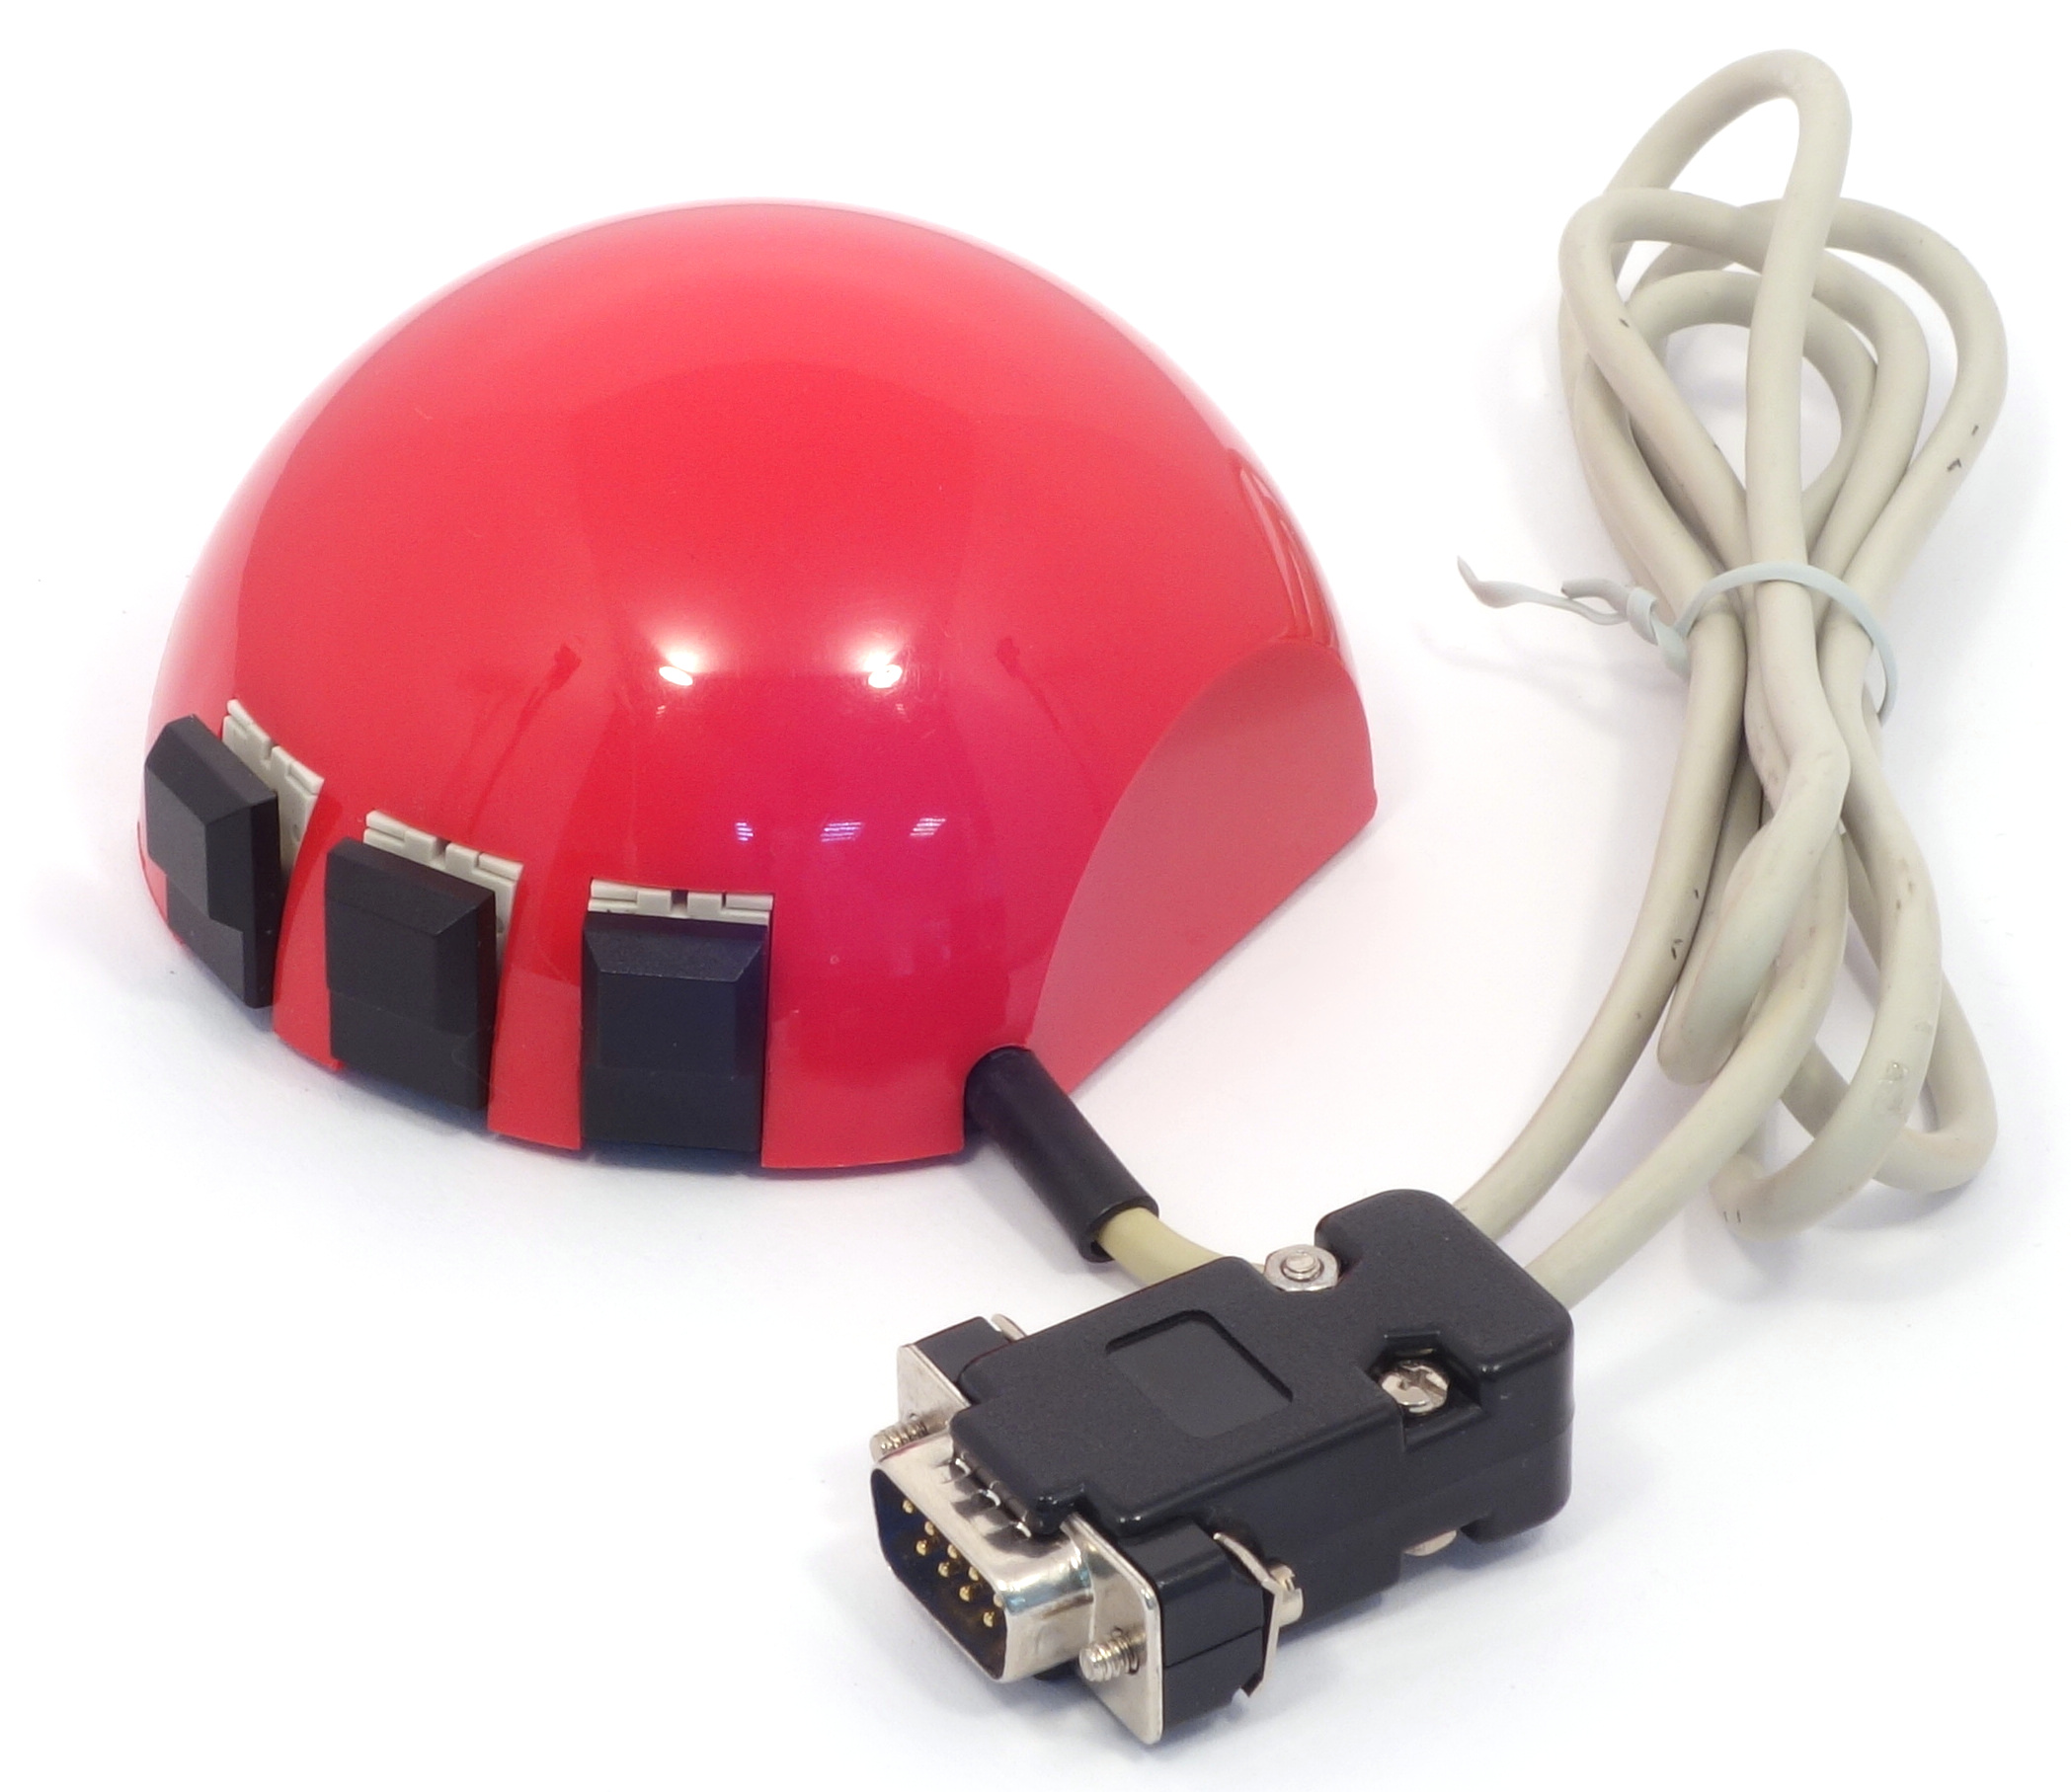
\includegraphics[scale=0.5]{1982_depraz_digimouse/pic_60.jpg}
    \caption{DIGIMOUSE}
    \label{fig:DIGIMOUSEP4Pic}
\end{figure}

The same mouse was branded in different variations as D\'epraz Mouse, Logitech P-4, DIGIMOUSE 1000 P (figure \ref{fig:DIGIMOUSEP4TopAndBottom}).

\begin{figure}[h]
    \centering
    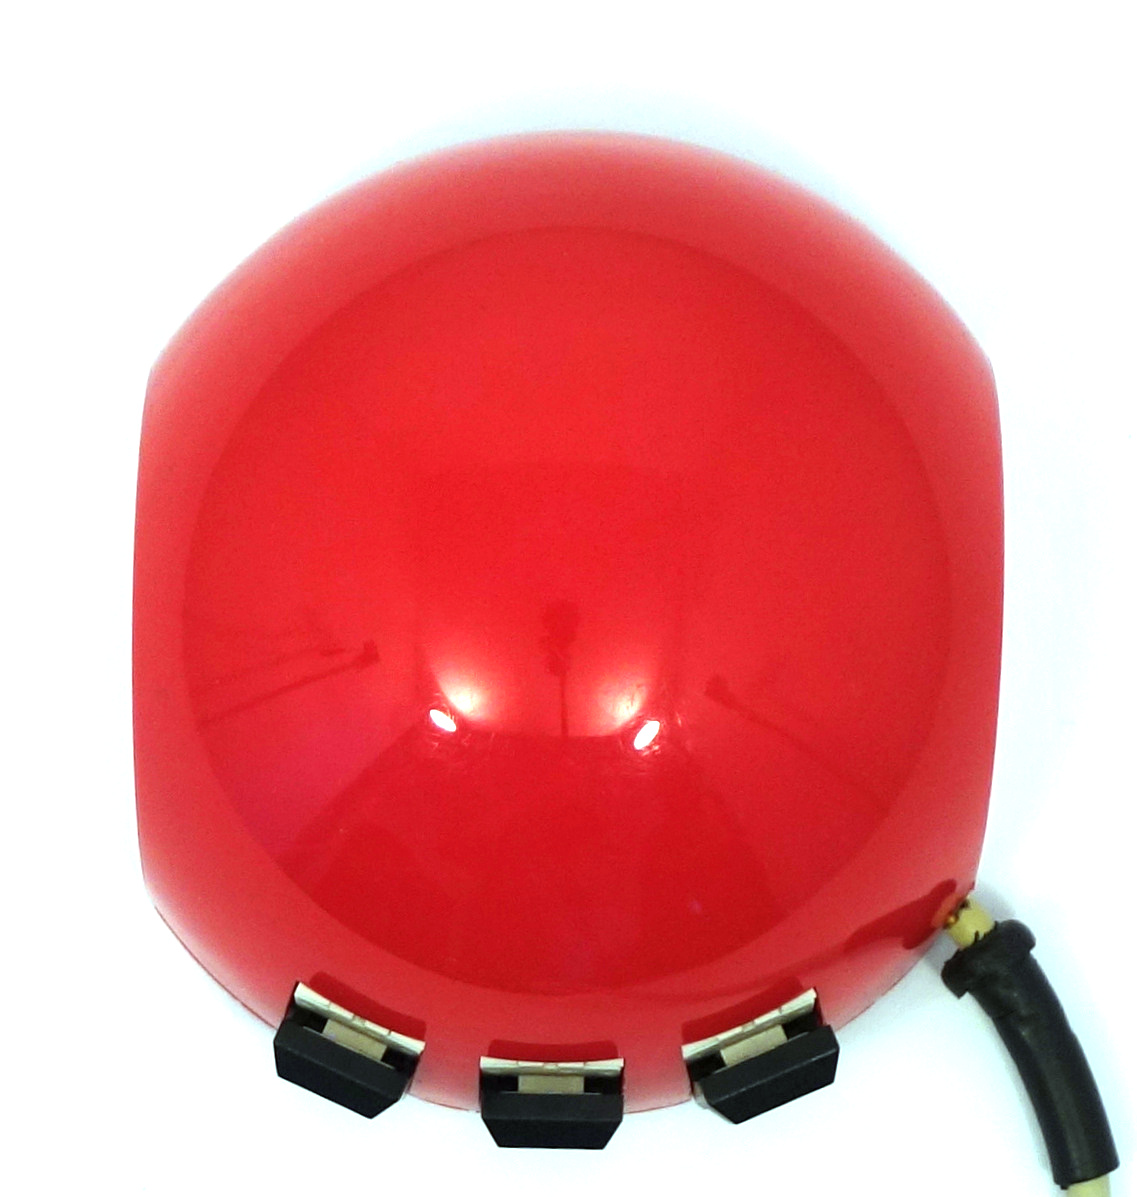
\includegraphics[scale=0.4]{1982_depraz_digimouse/top_60.jpg}
    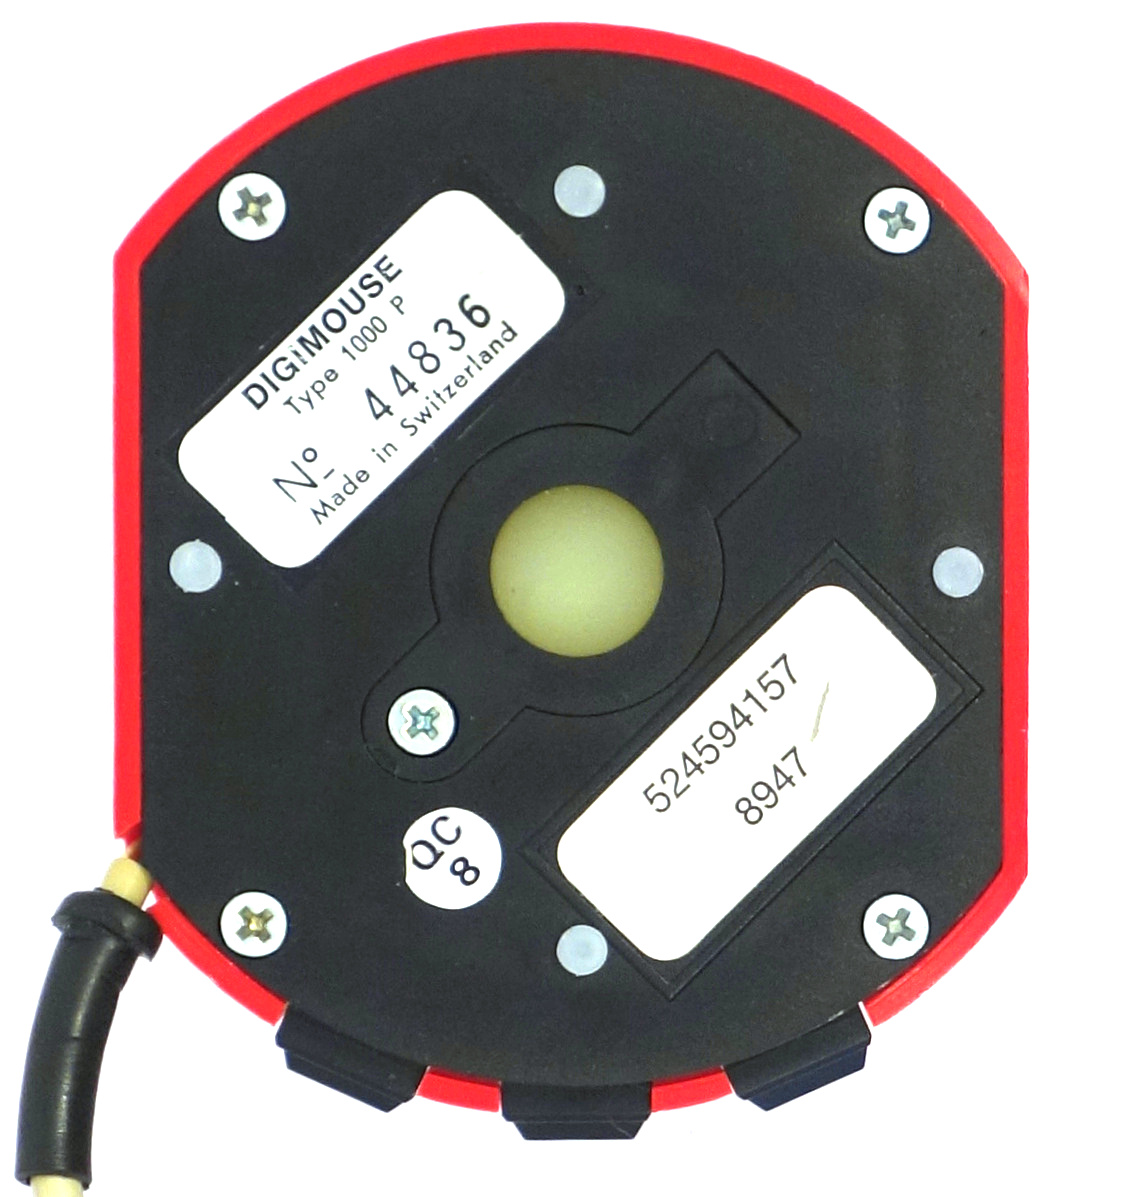
\includegraphics[scale=0.37]{1982_depraz_digimouse/bottom_60.jpg}
    \caption{DIGIMOUSE, top and bottom views}
    \label{fig:DIGIMOUSEP4TopAndBottom}
\end{figure}

The mouse has a typical size for mice of the 1980s (figure \ref{fig:DIGIMOUSEP4Size}).

\begin{figure}[h]
    \centering
    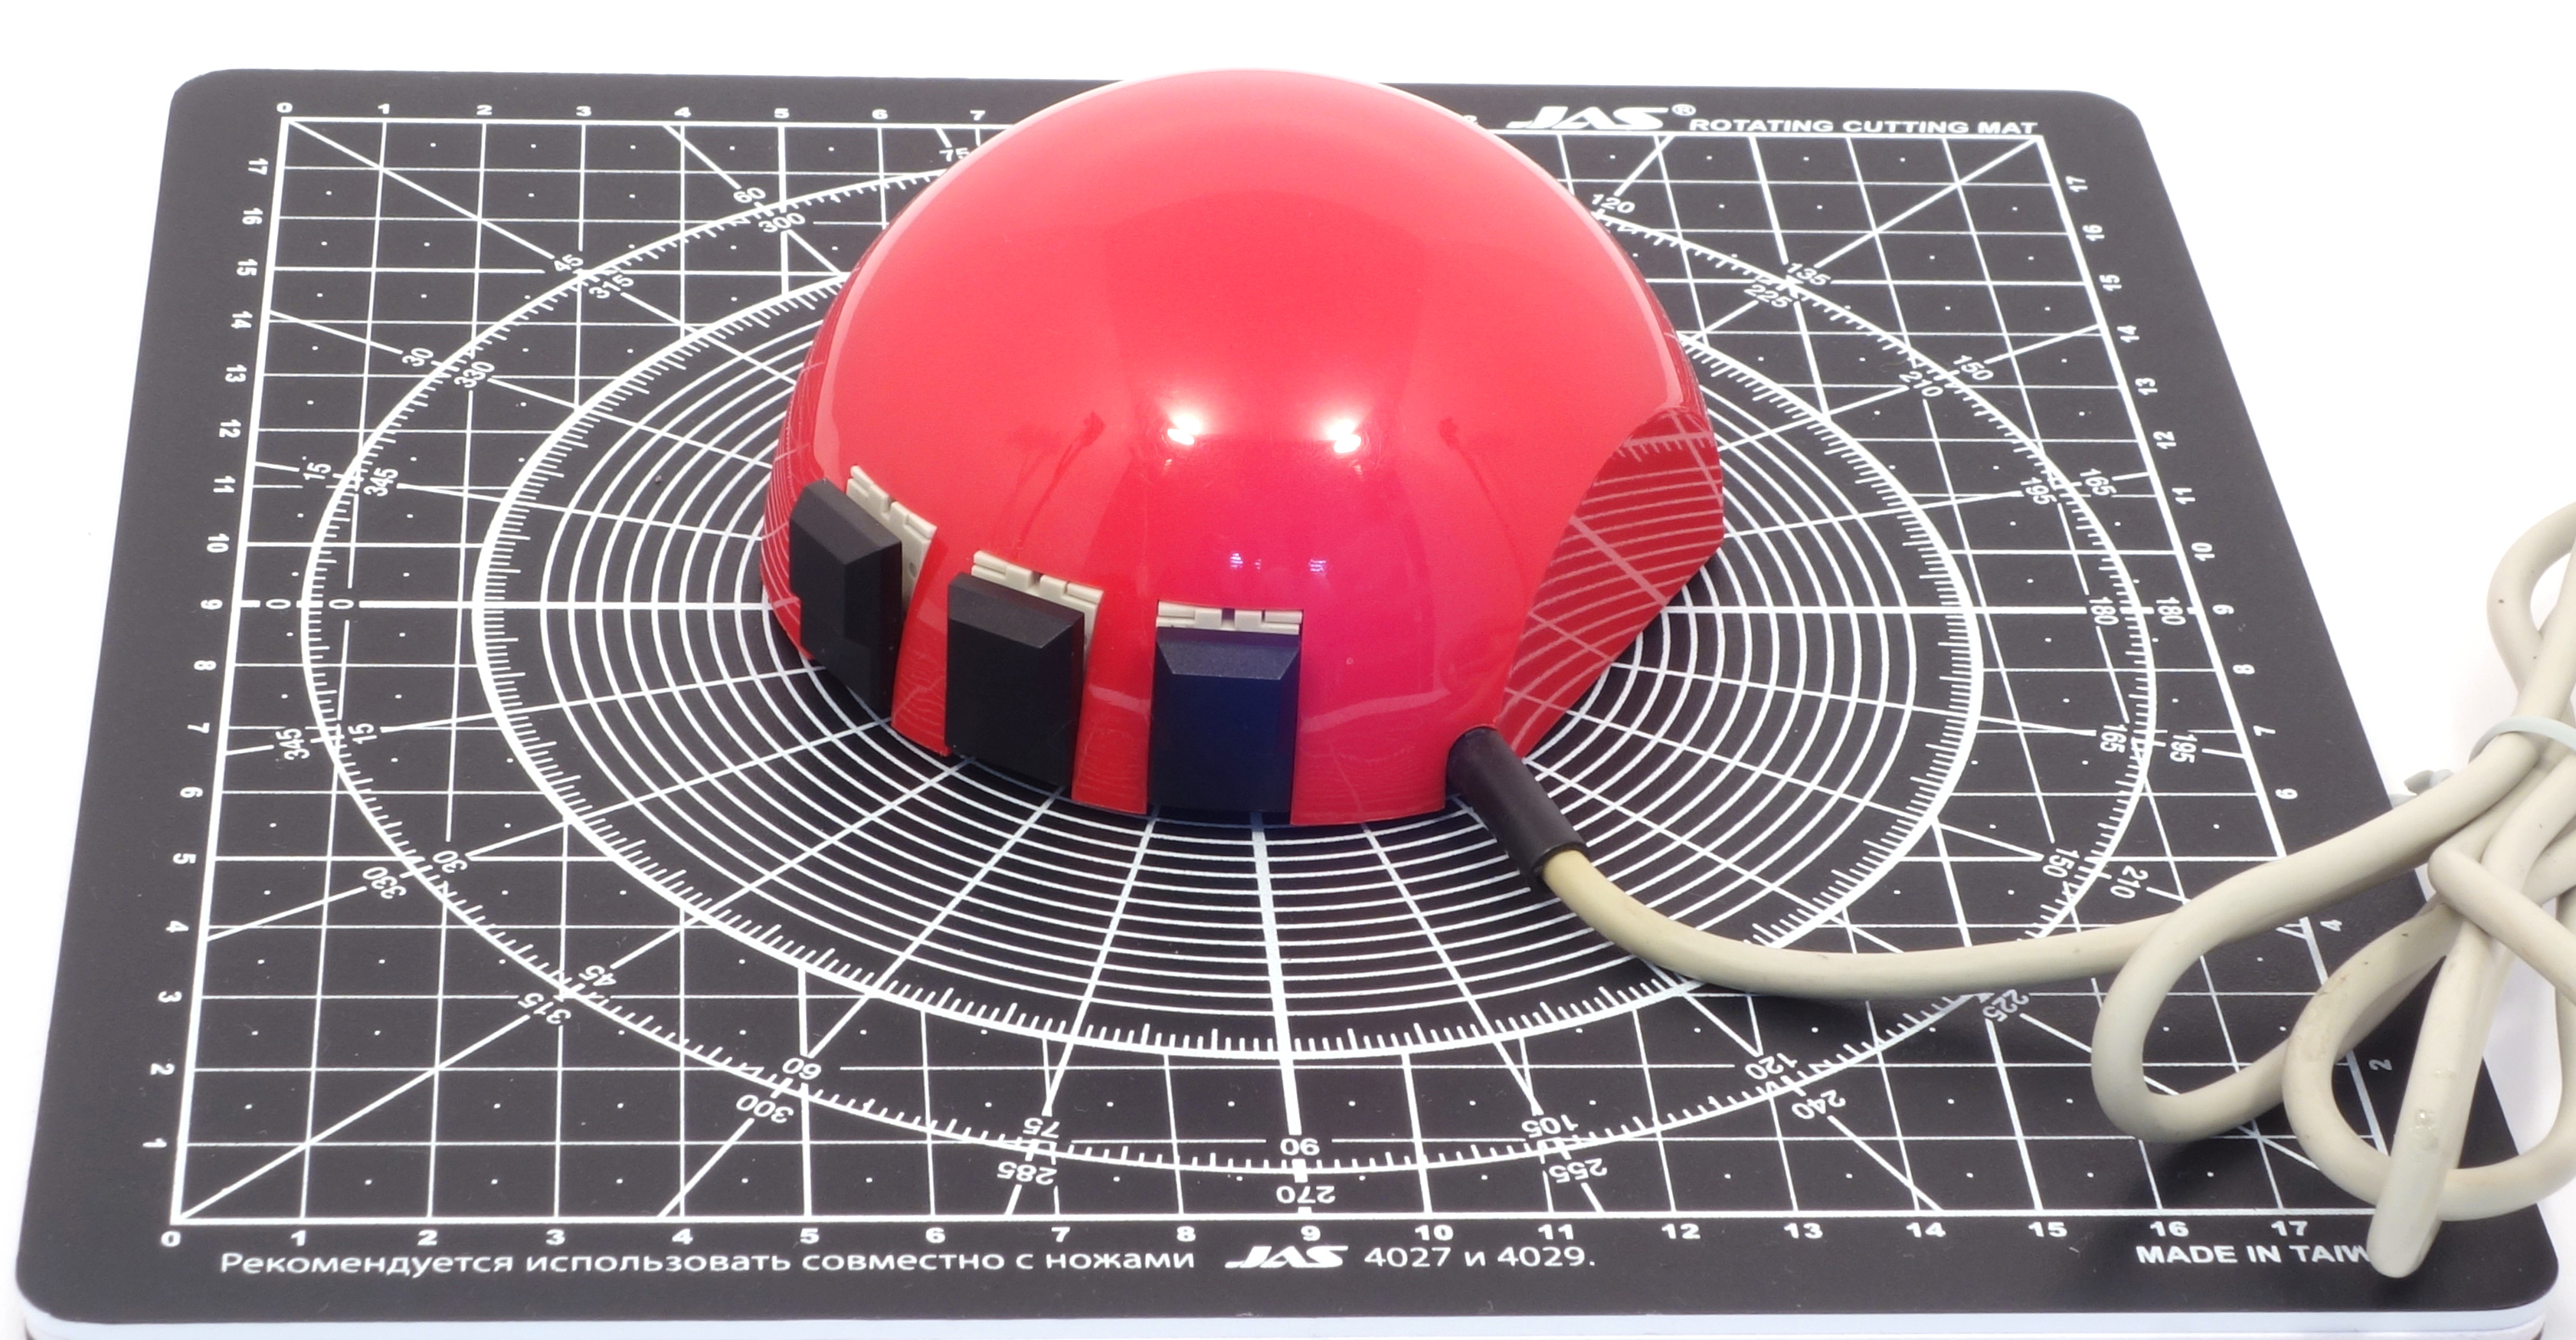
\includegraphics[scale=0.5]{1982_depraz_digimouse/size_30.jpg}
    \caption{DIGIMOUSE on a graduated pad with a grid step of 1~cm}
    \label{fig:DIGIMOUSEP4Size}
\end{figure}

The body is a 3 ½-inch hemisphere cut on the sides for easy thumb and pinky finger grip. Three spring-loaded buttons with a distinct click and tactile response to actuation are located vertically on the side of the case farthest from the user \cite{oldmouse}. Due to the fact that the buttons take up the entire front side of the case, the cable enters diagonally into the mouse. This shape was called ``dome'' and turned out to be one of the first truly successful mouse body shapes: geometric simplicity is combined with good ergonomics, making the mouse pleasant to hold in hand (figure \ref{fig:DIGIMOUSEP4Hand}). Owners of small hands can easily rest their wrist on the table or lift it up when necessary to use the buttons.

\begin{figure}[h]
    \centering
    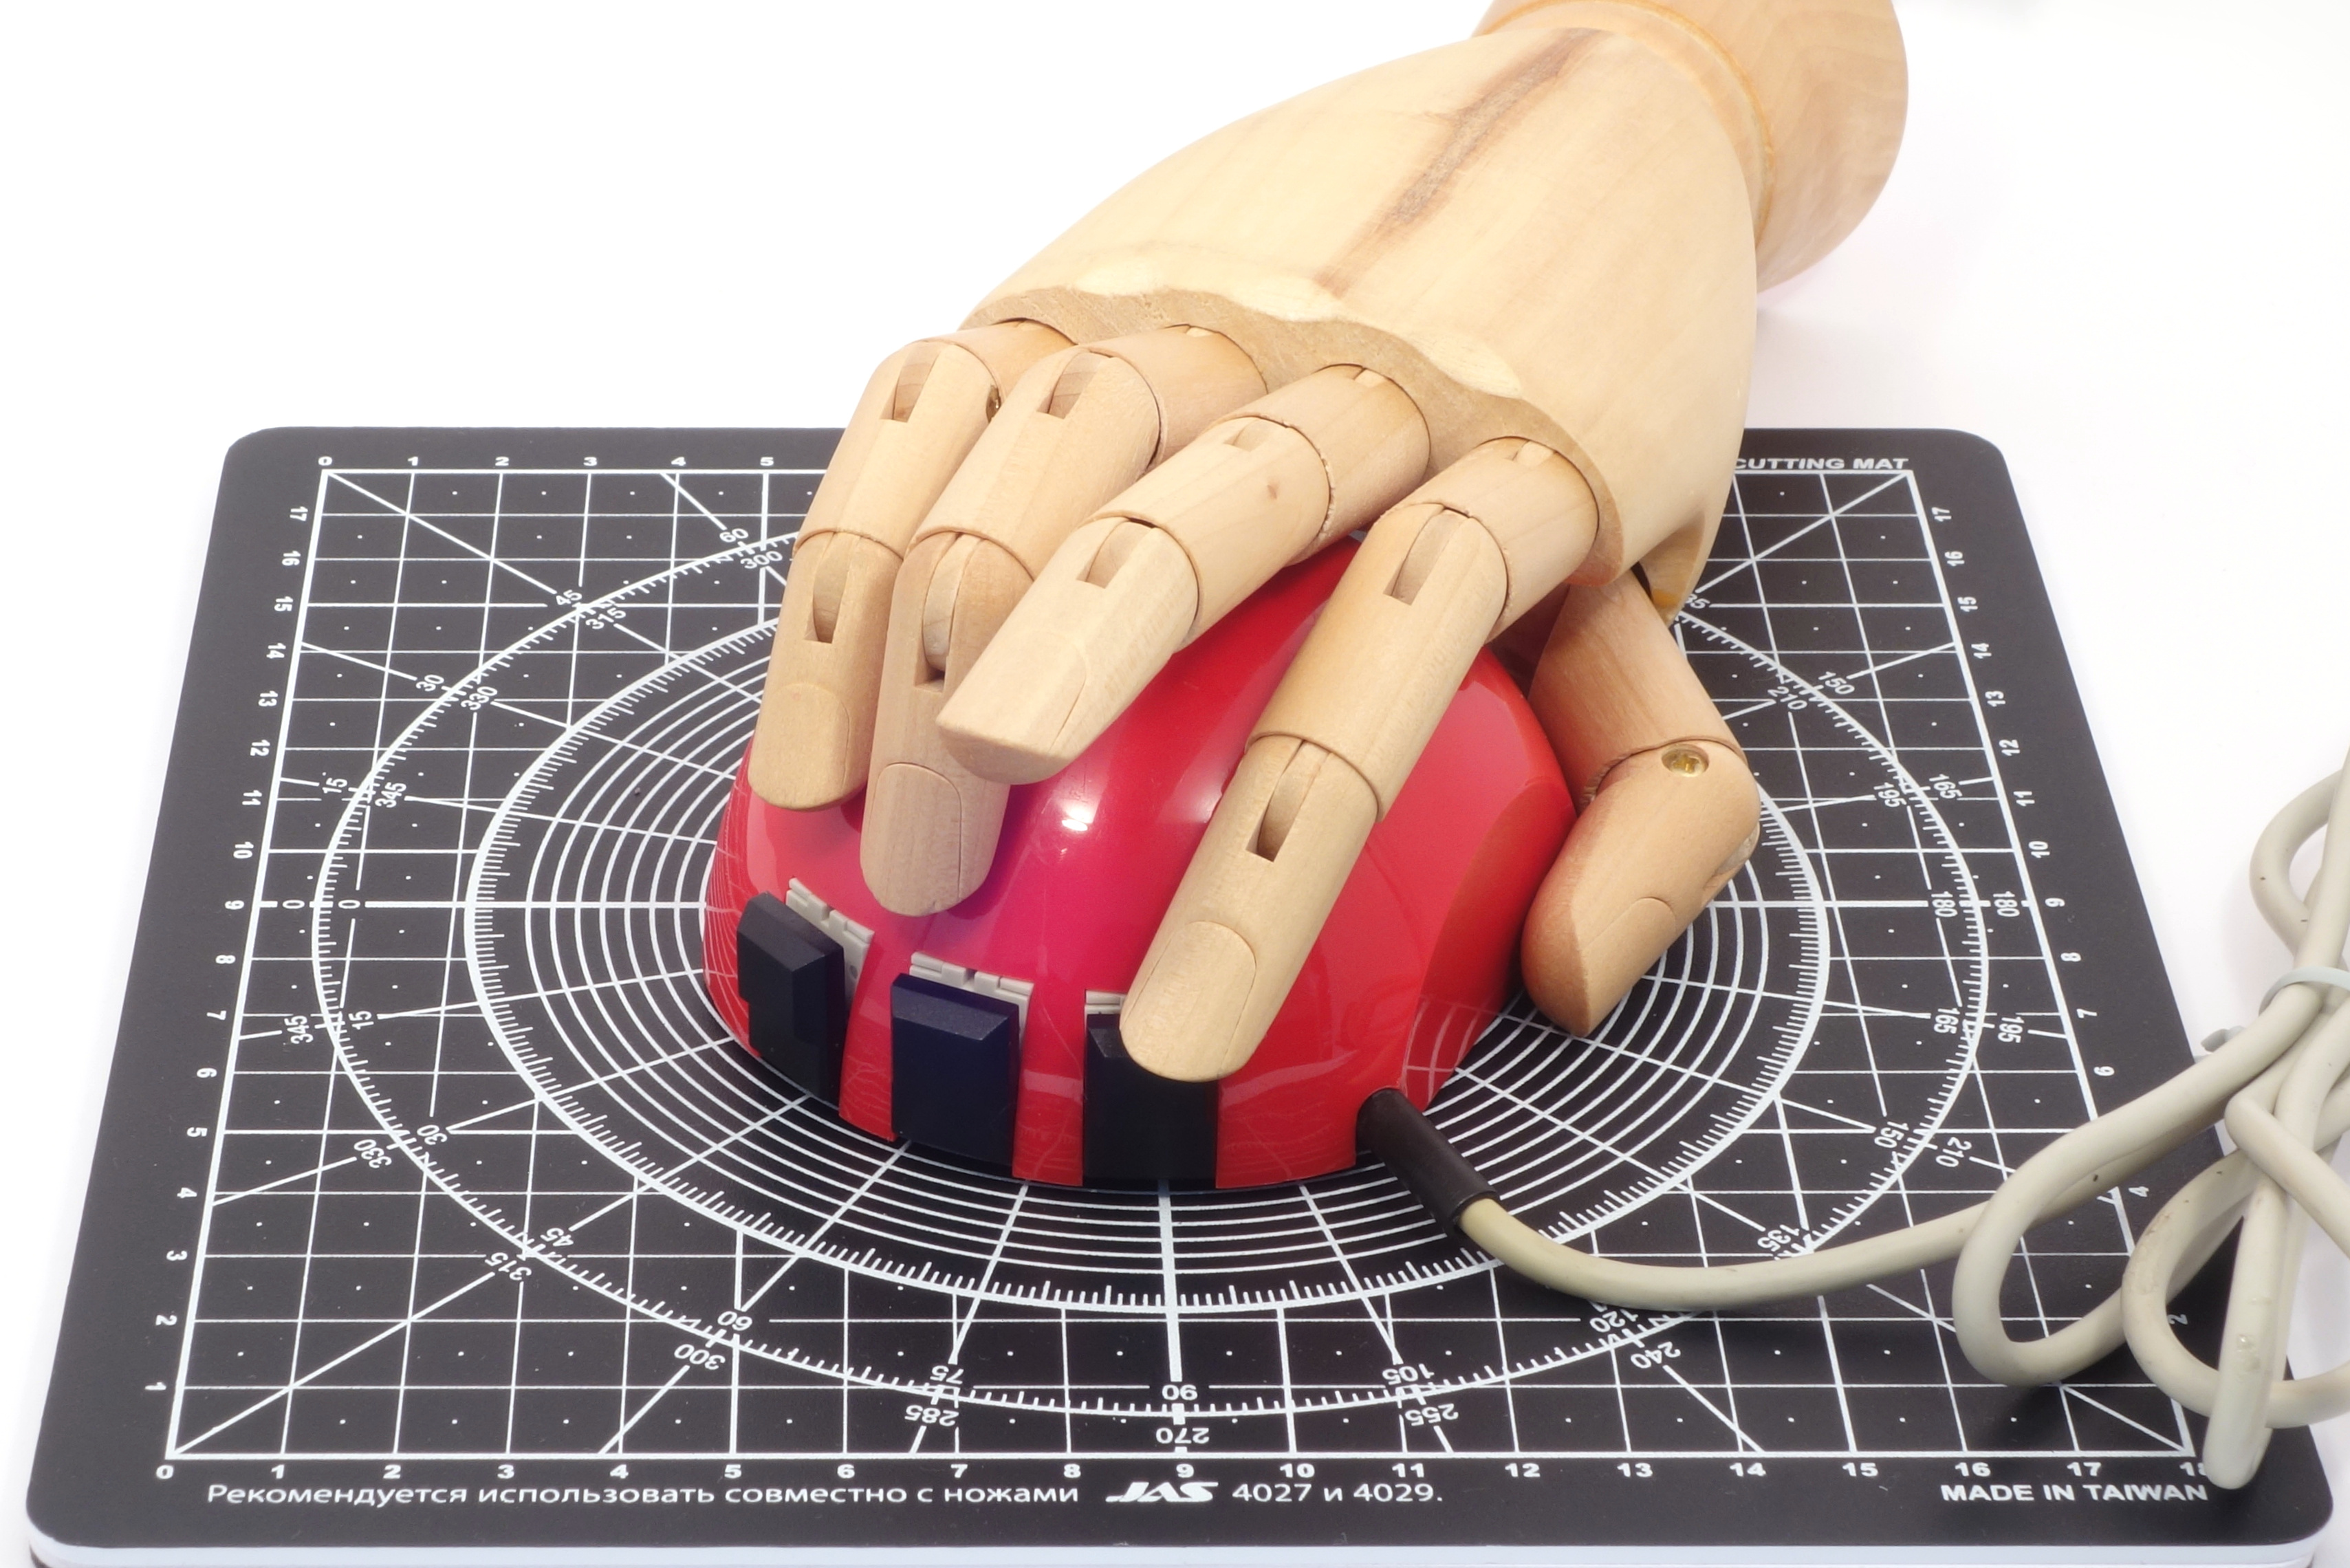
\includegraphics[scale=0.5]{1982_depraz_digimouse/hand_30.jpg}
    \caption{DIGIMOUSE with a human hand model}
    \label{fig:DIGIMOUSEP4Hand}
\end{figure}

The mouse has a 381 DPI resolution. Since 1984, as an additional accessory, these mice were sometimes equipped with a special LogiMate \cite{oldmouse} converter, which allowed the mouse to be connected not to a separate adapter with a bus interface, but to a keyboard cable. With this connected, moving the mouse resulted in generating cursor key codes:  the resolution was 12 keypresses per inch horizontally and 6 keypresses vertically by default, which was designed to work in 80x25 character text mode. PC Magazine's review noted that using a mouse in standard mode made it possible to move the cursor in a text editor seven times faster than using the corresponding keys on the keyboard (however, it took getting used to the fact that as a result of a slight movement of the mouse over the rightmost position, the text editor cursor immediately jumped to the left position of the next line). For obvious reasons, this use of the mouse did not require a driver; however, its use gave the possibility of additional settings "--- for example, it allowed to set the resolution of the LogiMate adapter in the range of 1--100 keypresses per inch, as well as reassign the action of the mouse keys (key codes F8, F9 and F10 were generated by default) \cite{DIGIMOUSE}.

 \begin{figure}[h]
    \centering
    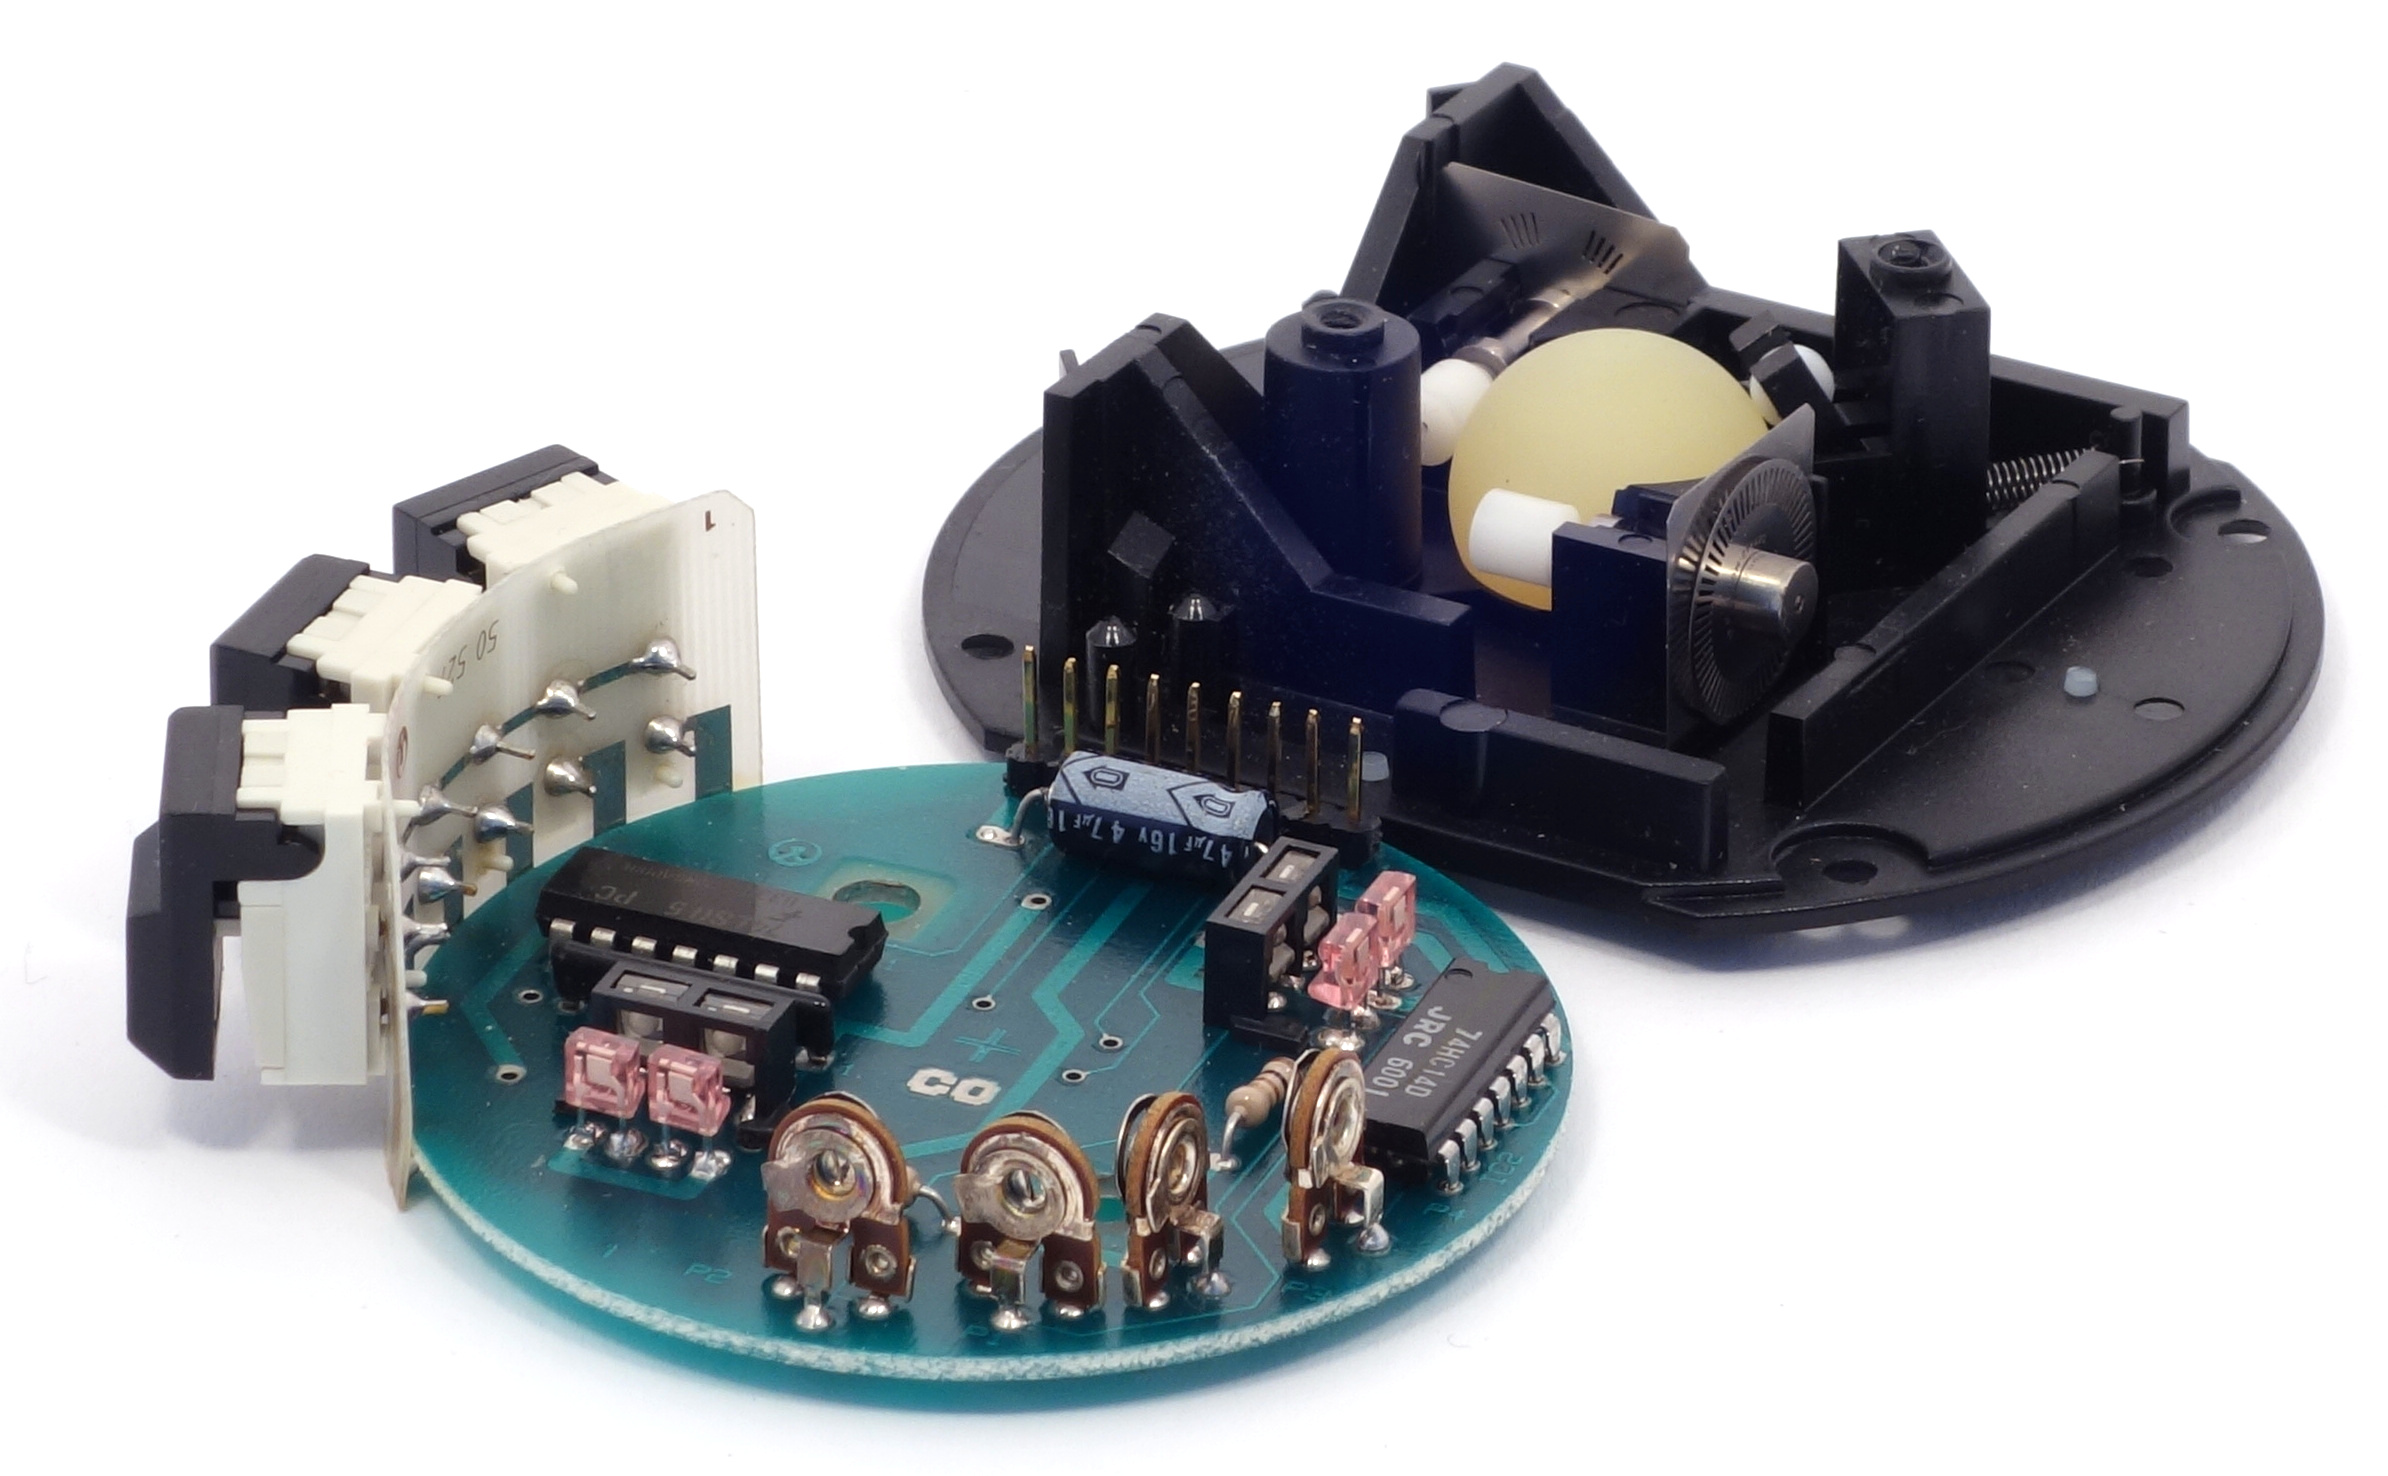
\includegraphics[scale=0.75]{1982_depraz_digimouse/inside_60.jpg}
    \caption{DIGIMOUSE disassembled}
    \label{fig:DIGIMOUSEP4Inside}
\end{figure}

The internal structure of the mouse is shown in figure \ref{fig:DIGIMOUSEP4Inside}. As already mentioned, this mouse uses optomechanical encoders. Optocouples are similar to those in mice from the 90s; however, the optical interrupter disk is made of metal and additionally equipped with a fixed mask that reduces the area of flare. During Logitech's production, the original design of the D\'epraz Mouse underwent some changes: in particular, the material of the roller cover and the original metal ball \cite{oldmouse} were replaced with plastic.

The most active sales of this mouse are from 1982 to 1984 (production ceased in the mid-80s with the release of the very popular inexpensive Logitech C7 model), and the original retail price was \$295. In a number of ways, the D\'epraz Mouse was a significantly more technologically advanced device than other mice of the first half of the 1980s. The combination of technological superiority, rather high price, and good ergonomics made this manipulator legendary. As a result of such popularity, in the first half of the 1990s, the "dome mouse" story continued unexpectedly with the release of two P4 clones: an almost complete visual copy from Sunnyline called Hit Mouse\cite{sunnyline}, as well as a transparent Crystal Clear Mouse manufactured by Suncom\cite{suncom}.

As you can see (figure \ref{fig:HitMousePic}), Hit Mouse is copying the exterior of P4 as close as possible. It was developed for the Amiga computers. In fact, the most noticeable change from DIGIMOUSE is the removable latch turnable ring cover of the ball, common in the 1990-s for being really handy to remove dirt and clean rollers.

\begin{figure}[h]
   \centering
    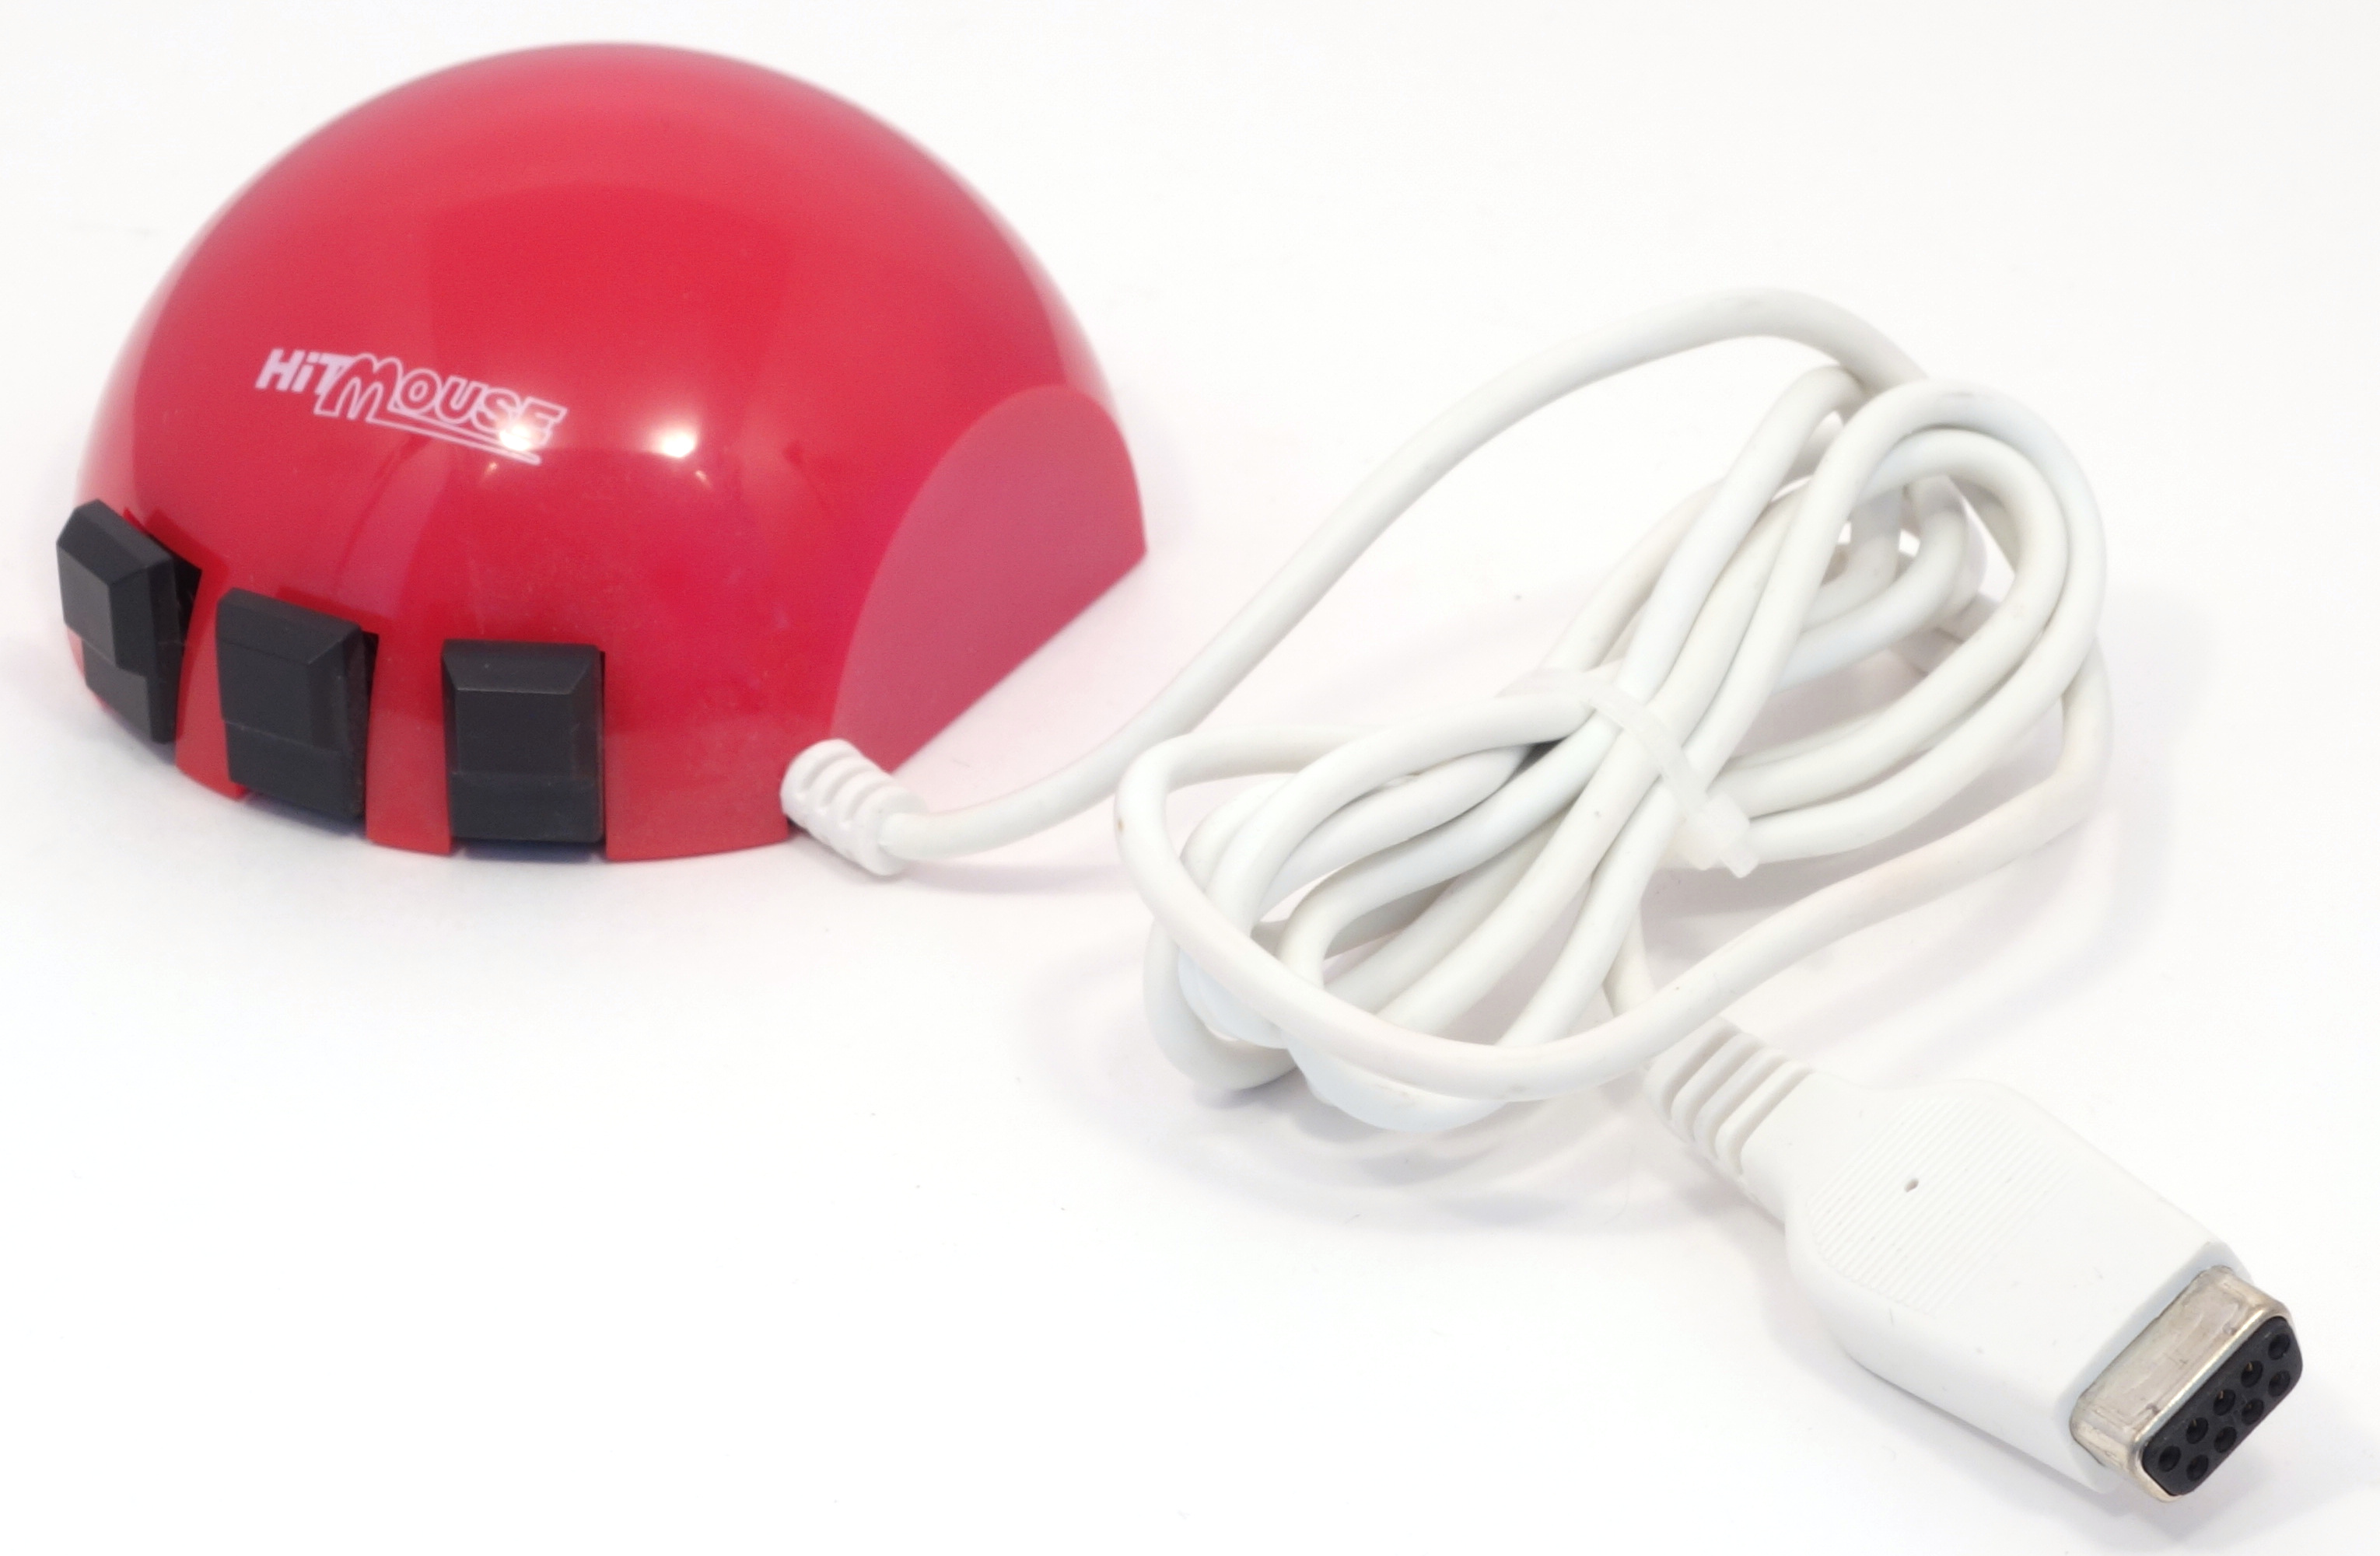
\includegraphics[scale=0.5]{1982_depraz_digimouse/hitmouse_pic_30.jpg}
    \caption{Sunnyline Hit Mouse}
    \label{fig:HitMousePic}
\end{figure}

Of course, the copying was only related to the exterior (the most common was the red case and black buttons, although the article in Amiga Kickstart also mentions \cite{sunnyline} a transparent version in addition to Suncom's variant). Internally, Hit Mouse is close to typical optomechanical mice of the mid-90s (figure \ref{fig:HitMouseInside}). Taking into account the fact that Hit Mouse was produced in 1991-1992, technically it can be considered a very relevant device for its time.

However, the domed shape, which proved to be an extremely successful solution among mice of the 80s, no longer aroused such enthusiasm among users of the 90s. The Amiga Kickstart short review described this design as very unusual, taking time to get used to \cite{sunnyline}.

 \begin{figure}[h]
    \centering
    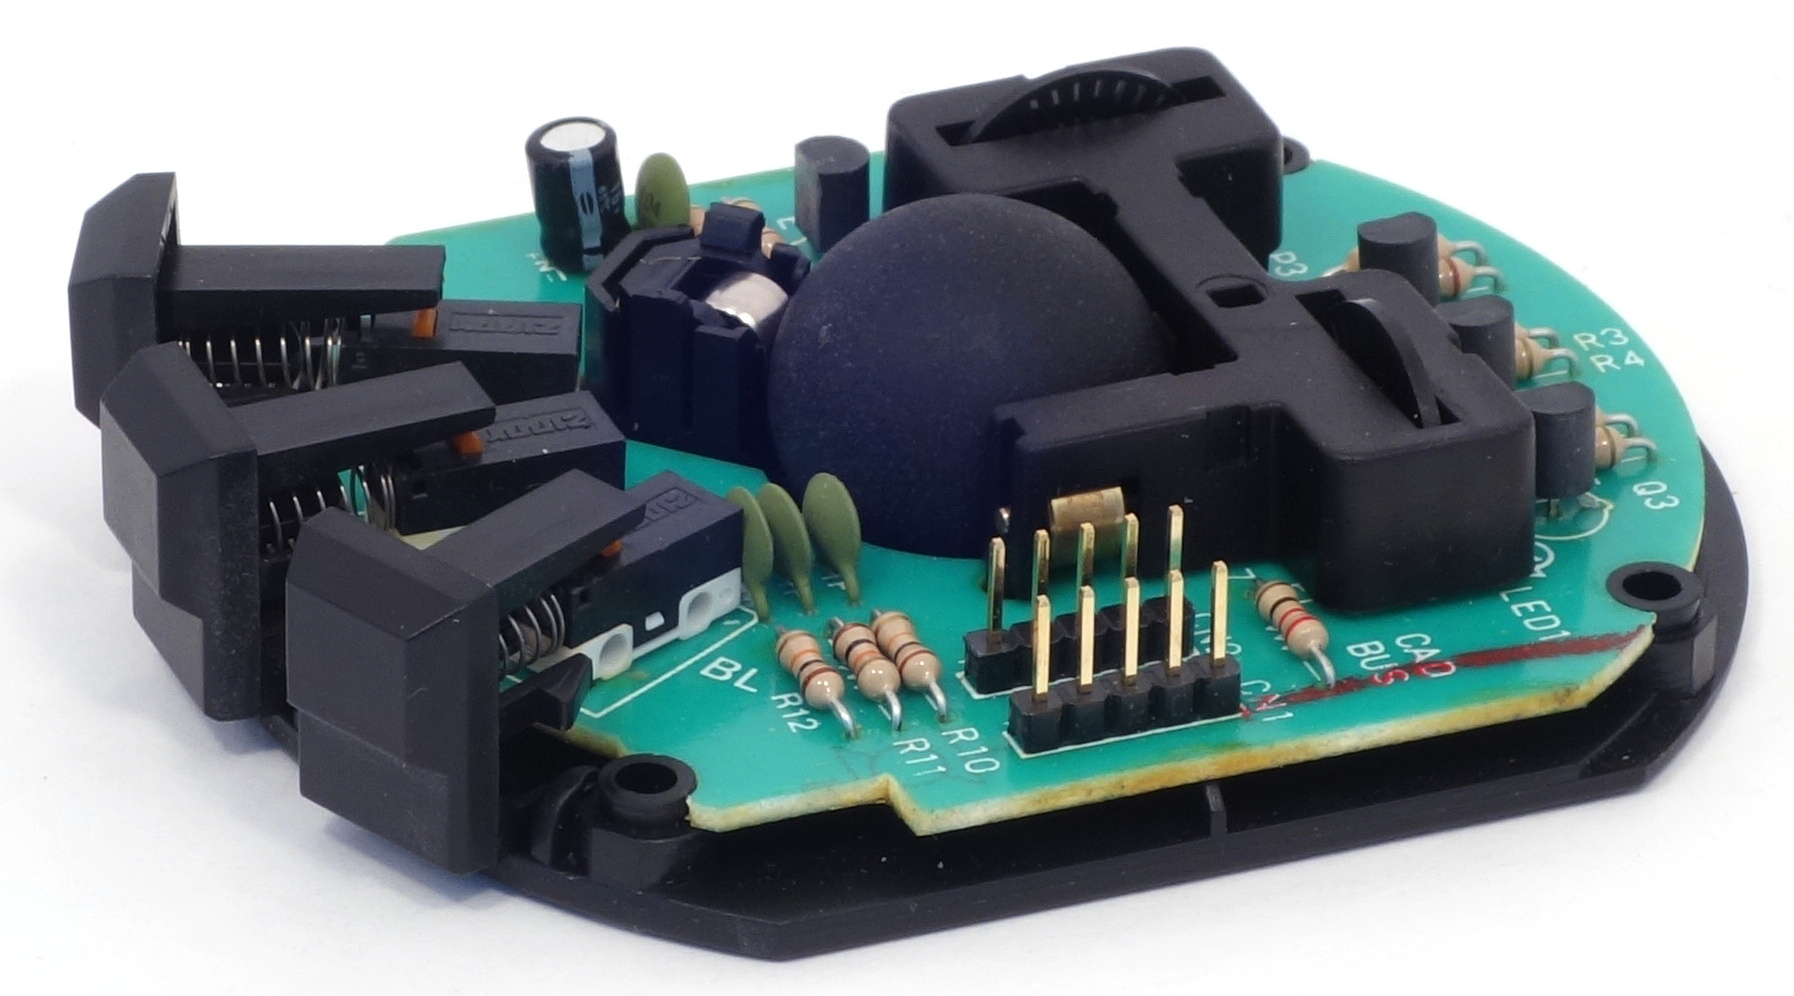
\includegraphics[scale=0.7]{1982_depraz_digimouse/hitmouse_inside_30.jpg}
    \caption{Sunnyline Hit Mouse disassembled}
    \label{fig:HitMouseInside}
\end{figure}

\begin{thebibliography}{9}
\bibitem {DIGIMOUSE} J. Taylor. Faster then a speeding cursor key. // PC Magazine, V. 3, No. 2, February 7, 1984. "--- p. 243-245 \url{https://archive.org/details/PC-Mag-1984-02-07/page/n243/mode/2up}
\bibitem {oldmouse} D\'epraz / Digimouse mouse $\sim$ oldmouse.com \url{https://web.archive.org/web/20211019061819/https://www.oldmouse.com/mouse/logitech/digimouse.shtml}
\bibitem {sunnyline} A. Kramer. PIEP-SHOW. M\"ause im Vergleich. Hit-Mouse II // Amiga Kickstart No. 10, Oktober, 1991. "--- p. 52-54 \url{https://archive.org/details/amiga-kickstart-91-10/page/52/mode/2up}
\bibitem {suncom} Crystal mouse, Suncom Technologies, 1991, USA. Mice Farm on Instagram. \url{https://www.instagram.com/p/CXYkzSpoqnL/}
\end{thebibliography}
\end{document}

\documentclass[11pt, a4paper]{article}
\usepackage{pdfpages}
\usepackage{parallel}
\usepackage[T2A]{fontenc}
\usepackage{ucs}
\usepackage[utf8x]{inputenc}
\usepackage[polish,english,russian]{babel}
\usepackage{hyperref}
\usepackage{rotating}
\usepackage[inner=2cm,top=1.8cm,outer=2cm,bottom=2.3cm,nohead]{geometry}
\usepackage{listings}
\usepackage{graphicx}
\usepackage{wrapfig}
\usepackage{longtable}
\usepackage{indentfirst}
\usepackage{array}
\usepackage{tikzsymbols}
\usepackage{soul}
\usepackage[ruled,vlined]{algorithm2e}
%\counterwithout{figure}{section} 

\usepackage{url}
\makeatletter
\g@addto@macro{\UrlBreaks}{\UrlOrds}
\makeatother

\newcolumntype{P}[1]{>{\raggedright\arraybackslash}p{#1}}
\frenchspacing
\usepackage{fixltx2e} %text sub- and superscripts
\usepackage{icomma} % коскі ў матэматычным рэжыме
\PreloadUnicodePage{4}

\newcommand{\longpage}{\enlargethispage{\baselineskip}}
\newcommand{\shortpage}{\enlargethispage{-\baselineskip}}

\def\switchlang#1{\expandafter\csname switchlang#1\endcsname}
\def\switchlangbe{
\let\saverefname=\refname%
\def\refname{Літаратура}%
\def\figurename{Іл.}%
}
\def\switchlangen{
\let\saverefname=\refname%
\def\refname{References}%
\def\figurename{Fig.}%
}
\def\switchlangru{
\let\saverefname=\refname%
\let\savefigurename=\figurename%
\def\refname{Литература}%
\def\figurename{Рис.}%
}

\hyphenation{admi-ni-stra-tive}
\hyphenation{ex-pe-ri-ence}
\hyphenation{fle-xi-bi-li-ty}
\hyphenation{Py-thon}
\hyphenation{ma-the-ma-ti-cal}
\hyphenation{re-ported}
\hyphenation{imp-le-menta-tions}
\hyphenation{pro-vides}
\hyphenation{en-gi-neering}
\hyphenation{com-pa-ti-bi-li-ty}
\hyphenation{im-pos-sible}
\hyphenation{desk-top}
\hyphenation{elec-tro-nic}
\hyphenation{com-pa-ny}
\hyphenation{de-ve-lop-ment}
\hyphenation{de-ve-loping}
\hyphenation{de-ve-lop}
\hyphenation{da-ta-ba-se}
\hyphenation{plat-forms}
\hyphenation{or-ga-ni-za-tion}
\hyphenation{pro-gramming}
\hyphenation{in-stru-ments}
\hyphenation{Li-nux}
\hyphenation{sour-ce}
\hyphenation{en-vi-ron-ment}
\hyphenation{Te-le-pathy}
\hyphenation{Li-nux-ov-ka}
\hyphenation{Open-BSD}
\hyphenation{Free-BSD}
\hyphenation{men-ti-on-ed}
\hyphenation{app-li-ca-tion}

\def\progref!#1!{\texttt{#1}}
\renewcommand{\arraystretch}{2} %Іначай формулы ў матрыцы зліпаюцца з лініямі
\usepackage{array}

\def\interview #1 (#2), #3, #4, #5\par{

\section[#1, #3, #4]{#1 -- #3, #4}
\def\qname{LVEE}
\def\aname{#1}
\def\q ##1\par{{\noindent \bf \qname: ##1 }\par}
\def\a{{\noindent \bf \aname: } \def\qname{L}\def\aname{#2}}
}

\def\interview* #1 (#2), #3, #4, #5\par{

\section*{#1\\{\small\rm #3, #4. #5}}
\ifx\ParallelWhichBox\undefined%
    \addcontentsline{toc}{section}{#1, #3, #4}%
\else%
\ifnum\ParallelWhichBox=0%
    \addcontentsline{toc}{section}{#1, #3, #4}%
\fi\fi%

\def\qname{LVEE}
\def\aname{#1}
\def\q ##1\par{{\noindent \bf \qname: ##1 }\par}
\def\a{{\noindent \bf \aname: } \def\qname{L}\def\aname{#2}}
}

\newcommand{\interviewfooter}[1]{
\vskip 1em
\noindent \textit{#1}
}

\switchlang{en}
\begin{document}

\title{1983 "--- Apple Lisa mouse}
\date{}
\maketitle
\selectlanguage{english}
The Apple Lisa mouse was released in 1983 \cite{mouses} and is considered one of the first commercially available computer mice (figure \ref{fig:AppleLisaPic}).

\begin{figure}[h]
   \centering
    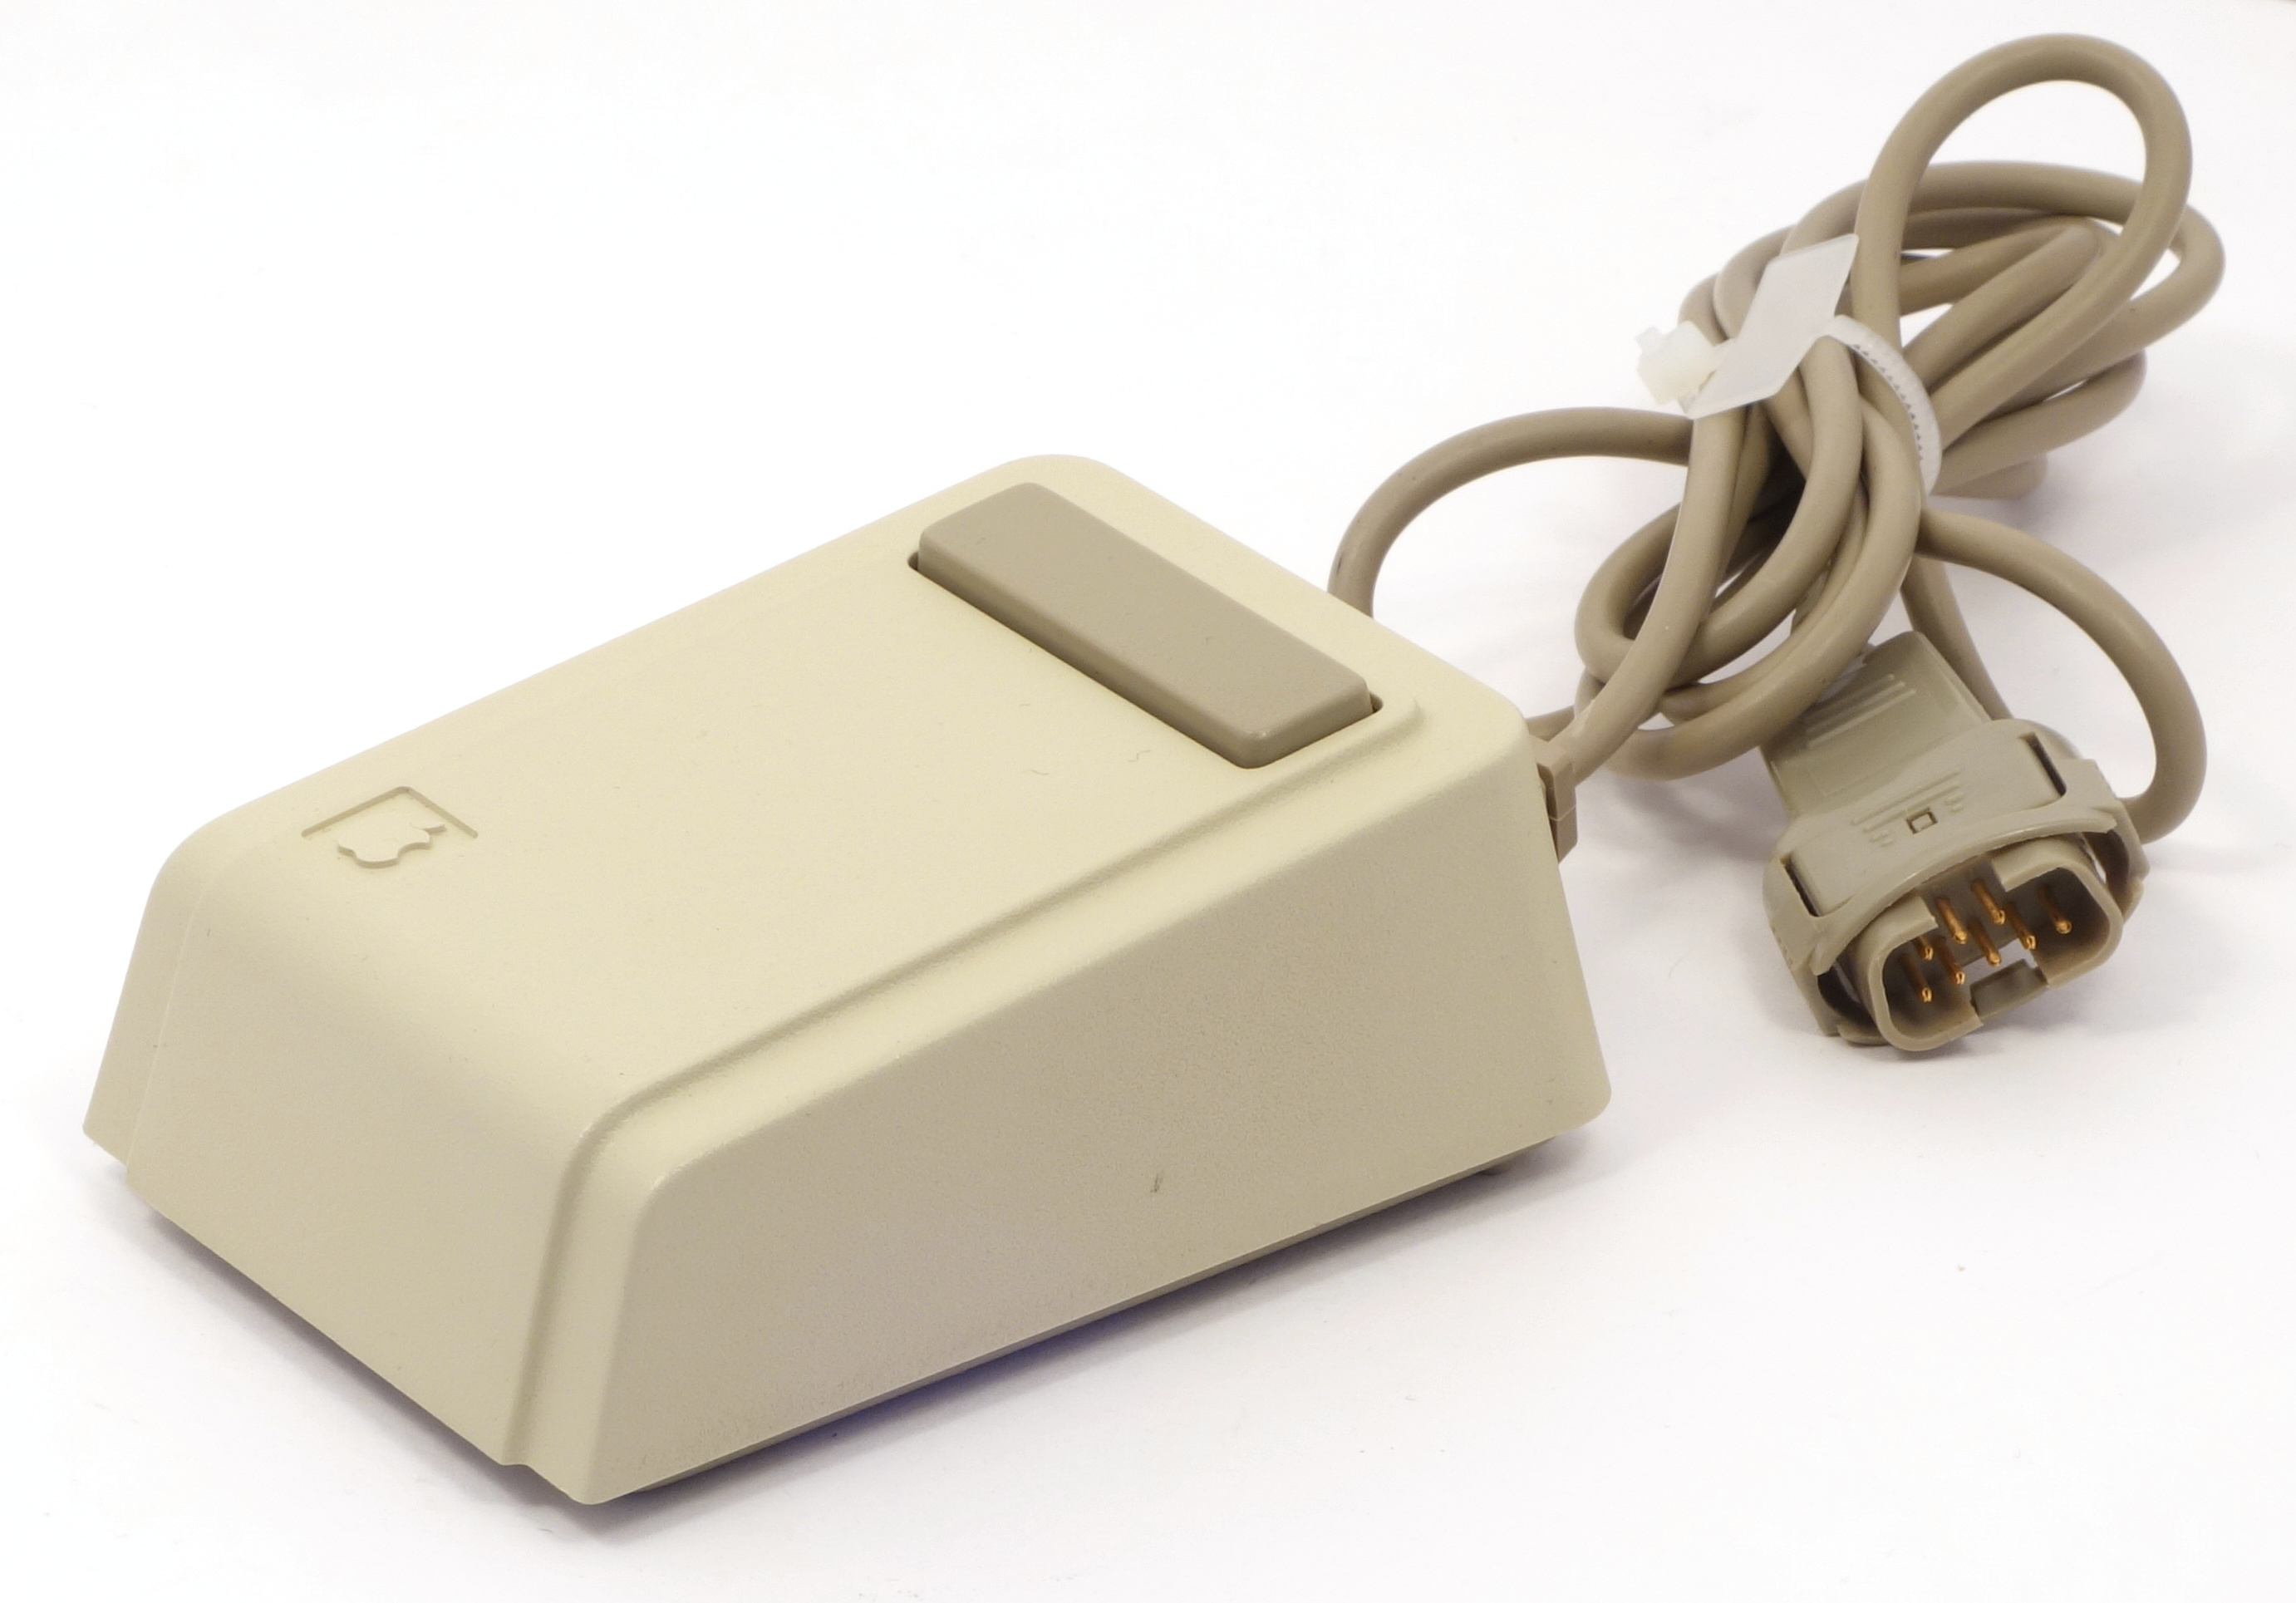
\includegraphics[scale=0.5]{1983_apple_lisa_mouse/applenorm_30.jpg}
    \caption{Apple Lisa mouse}
    \label{fig:AppleLisaPic}
\end{figure}

The mouse was manufactured by Apple, but the authorship of its development belongs to a third-party company, Hovey-Kelley (later renamed to IDEO). Based on the design of Xerox and Hawley Mouse House mice, the design team created a cheaper yet technically better mechanical part, and a complex internal structure of the case that holds the mouse parts together. Much attention was paid to other key components of the mouse, including the acoustic and tactile feel of the button and the rubberized coating on the ball \cite{ideo}.

\begin{figure}[h]
    \centering
    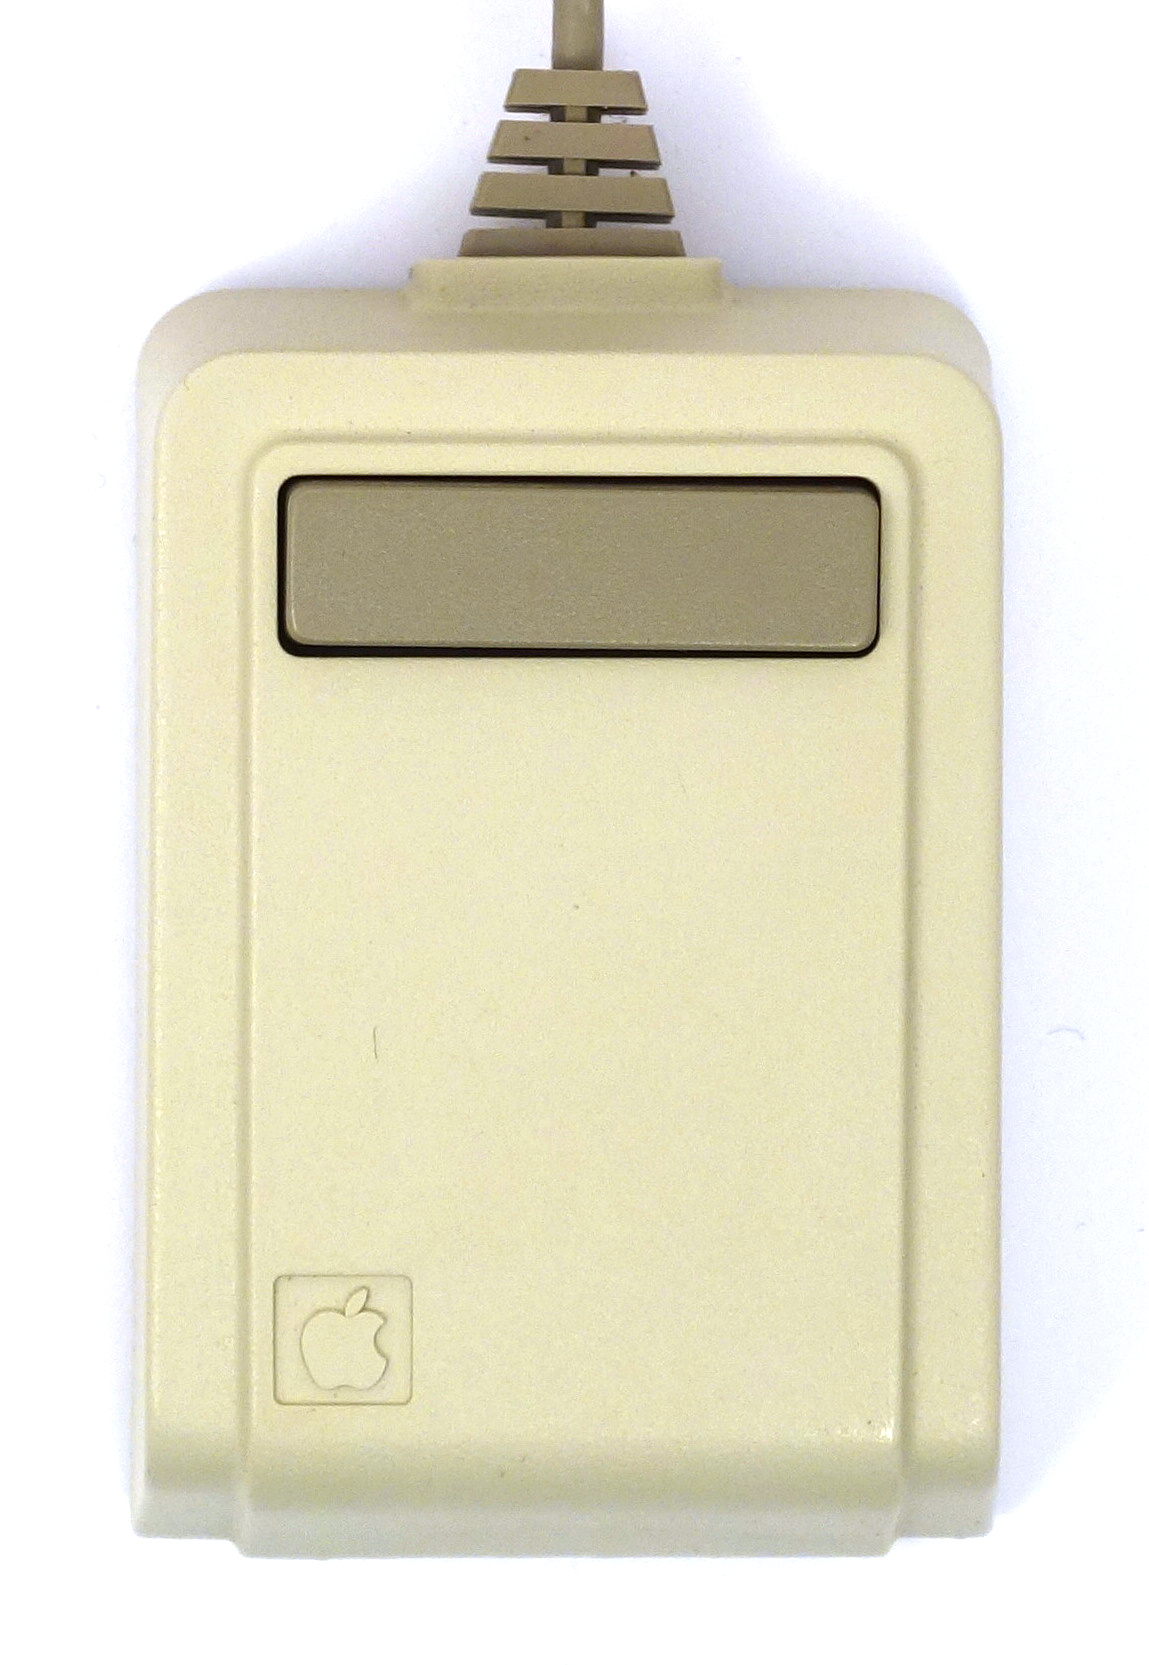
\includegraphics[scale=0.55]{1983_apple_lisa_mouse/appletop_60.jpg}
    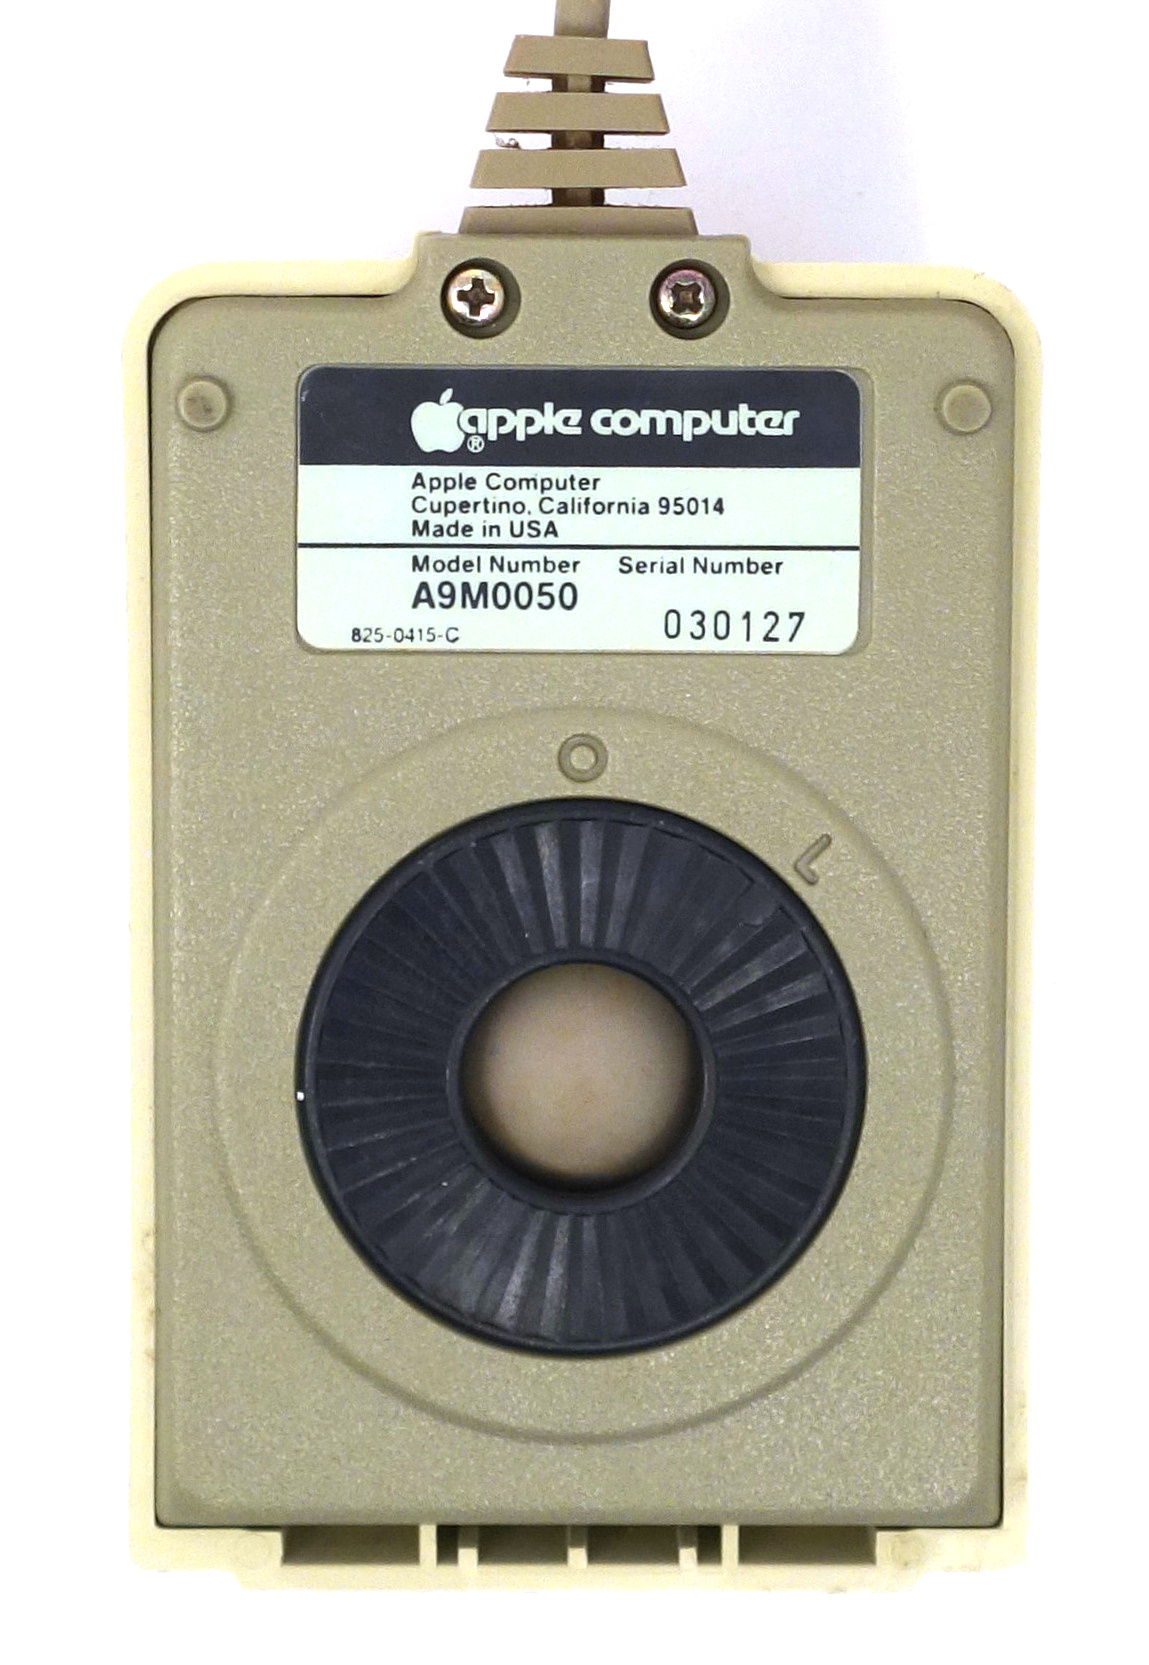
\includegraphics[scale=0.55]{1983_apple_lisa_mouse/applebottom_60.jpg}
    \caption{Apple Lisa mouse, top and bottom views}
    \label{fig:AppleLisaTopAndBottom}
\end{figure}

The body of the Lisa mouse is a beige slanted box. The underside of the mouse body, cable and button are brown. There is an embossed Apple logo on the case (figure \ref{fig:AppleLisaTopAndBottom}). The ball is made of metal and has a rubber coating for better grip, unlike earlier mice that had either a rubber or smooth steel ball. Later, a similar implementation of the ball will become the standard, as well as a removable ring that allows the user to easily remove the ball to clean the mouse from the collected debris, will become the standard. The same can be said about the basic design of its mechanism, which was later used in the vast majority of optomechanical mice.

\begin{figure}[h]
    \centering
    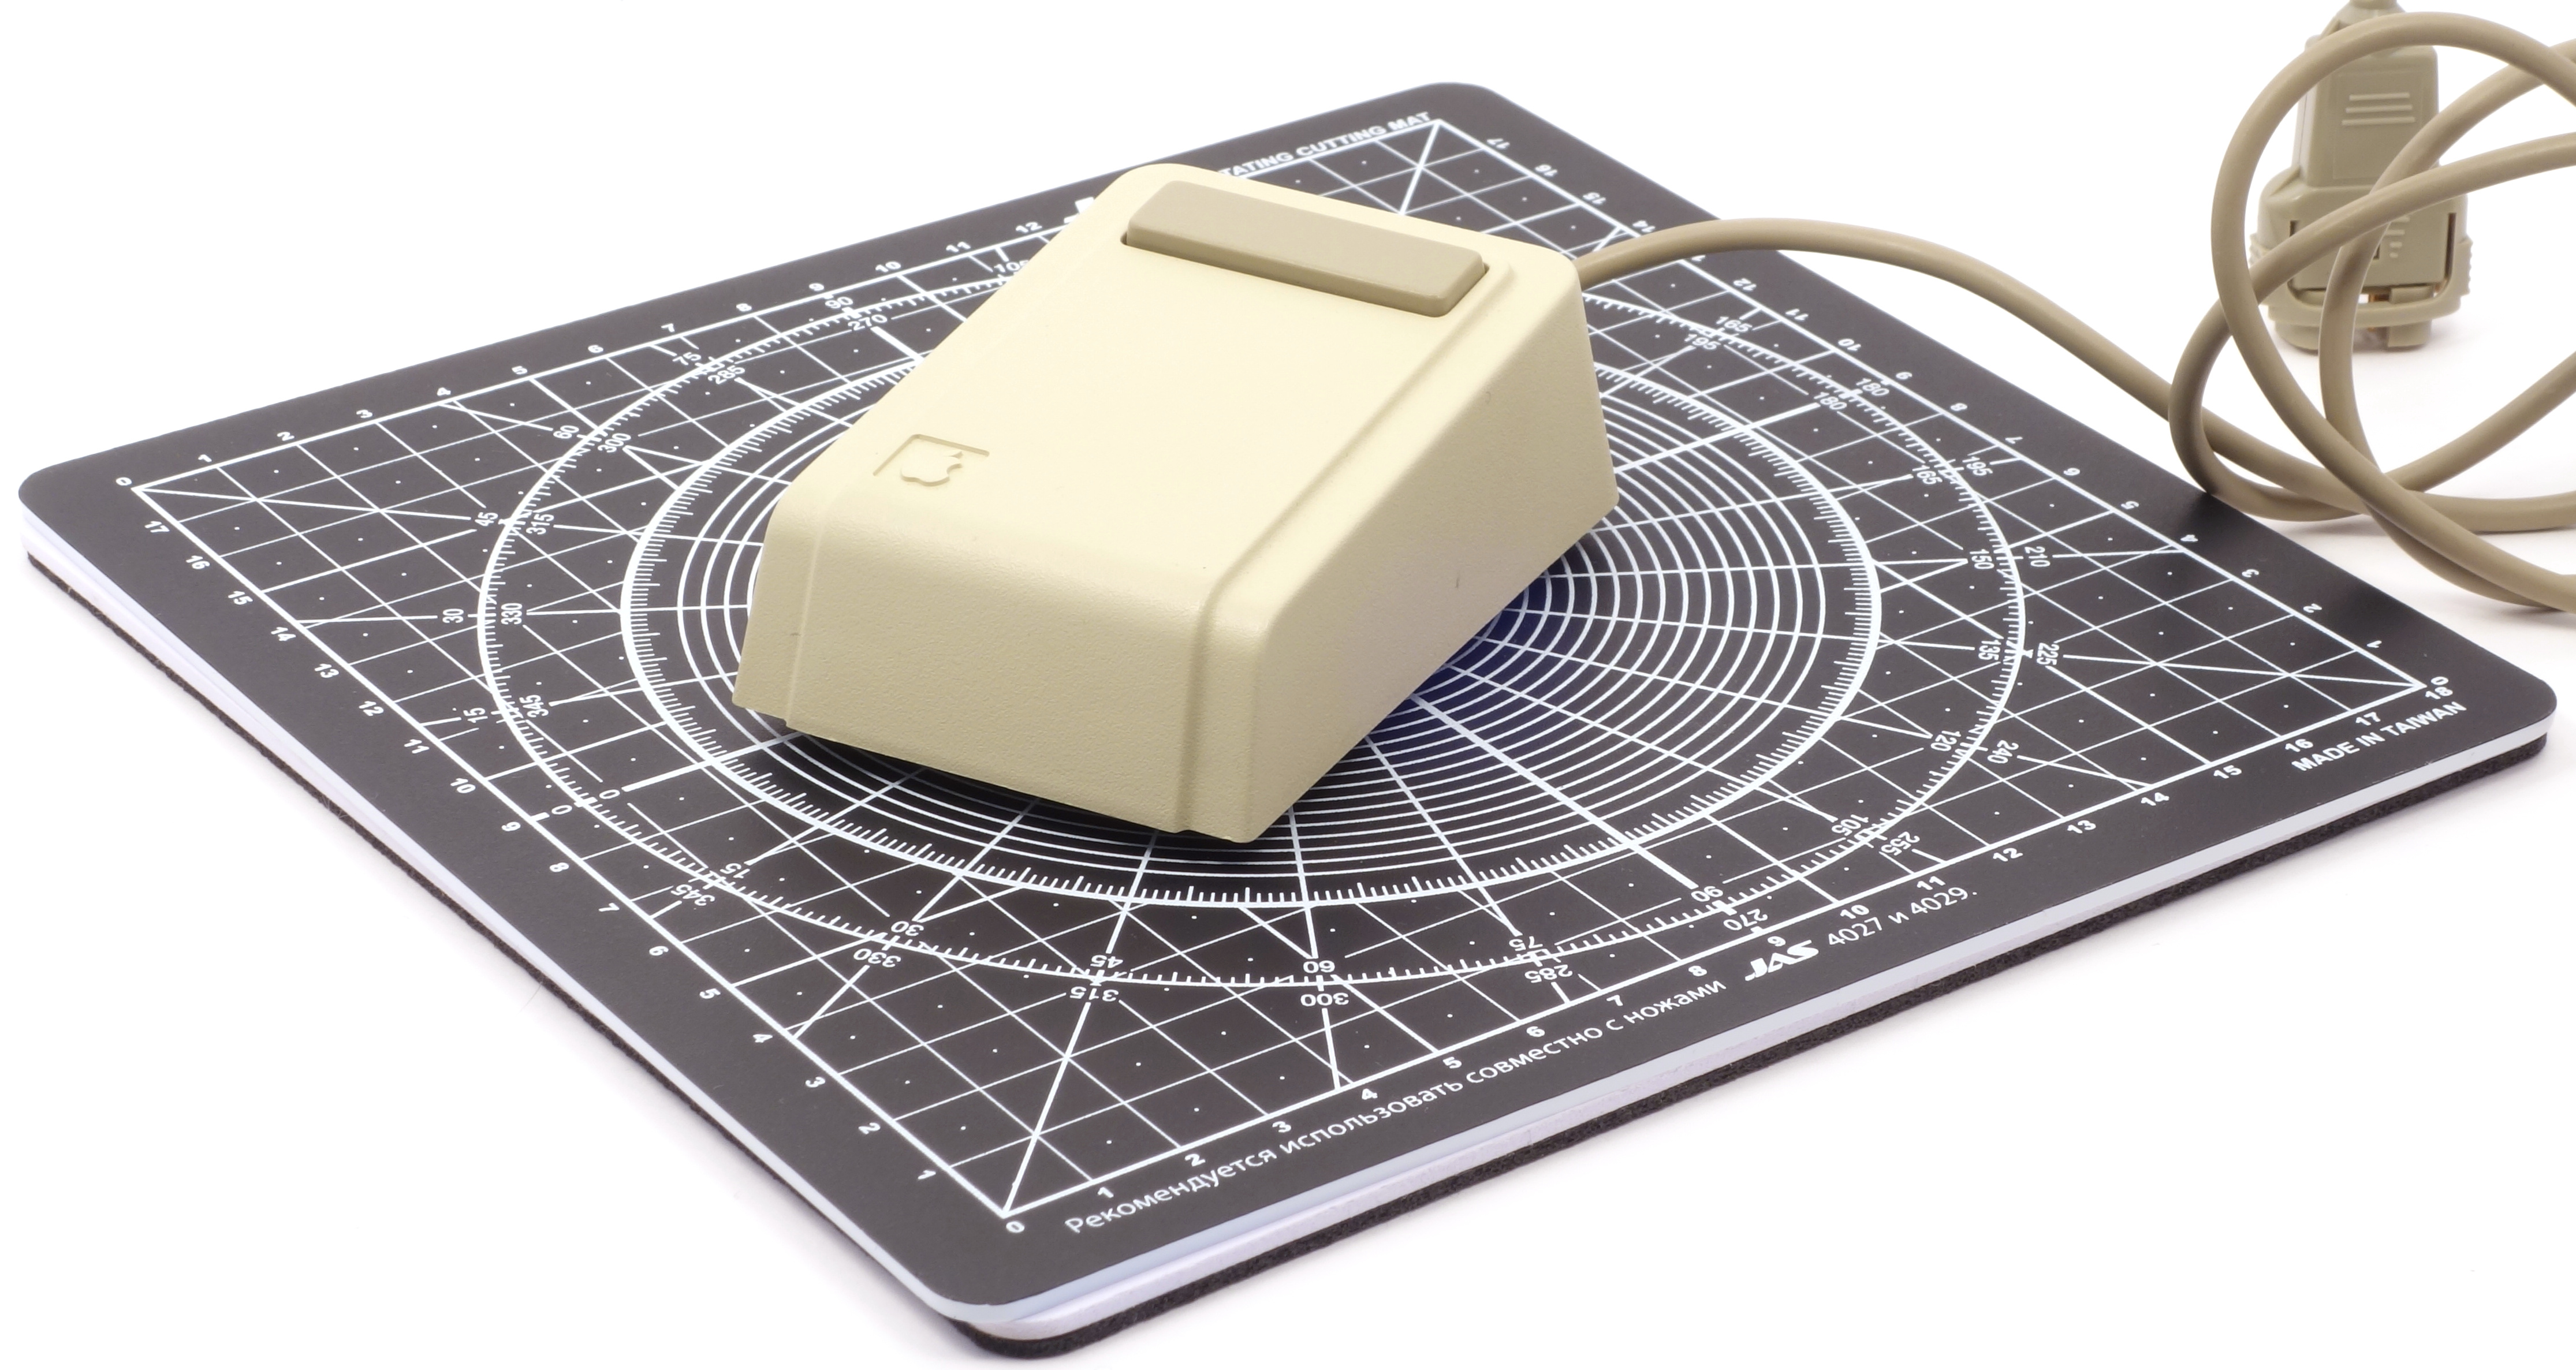
\includegraphics[scale=0.4]{1983_apple_lisa_mouse/applekovrik_60.jpg}
    \caption{Apple Lisa mouse on a graduated pad with a grid step of 1~cm}
    \label{fig:AppleLisaSize}
\end{figure}

Despite the relatively small size, however, typical of the mice of the 1980s (figure \ref{fig:AppleLisaSize}), the research of its developers has been useful, so it fits comfortably in the hand. At the same time, the only button is located orthogonally to the cable and is designed to be pressed with two fingers rather than one (figure \ref{fig:AppleLisaHand}), and the tactility of pressing is provided by a specially provided spring mechanism.

\begin{figure}[h]
    \centering
    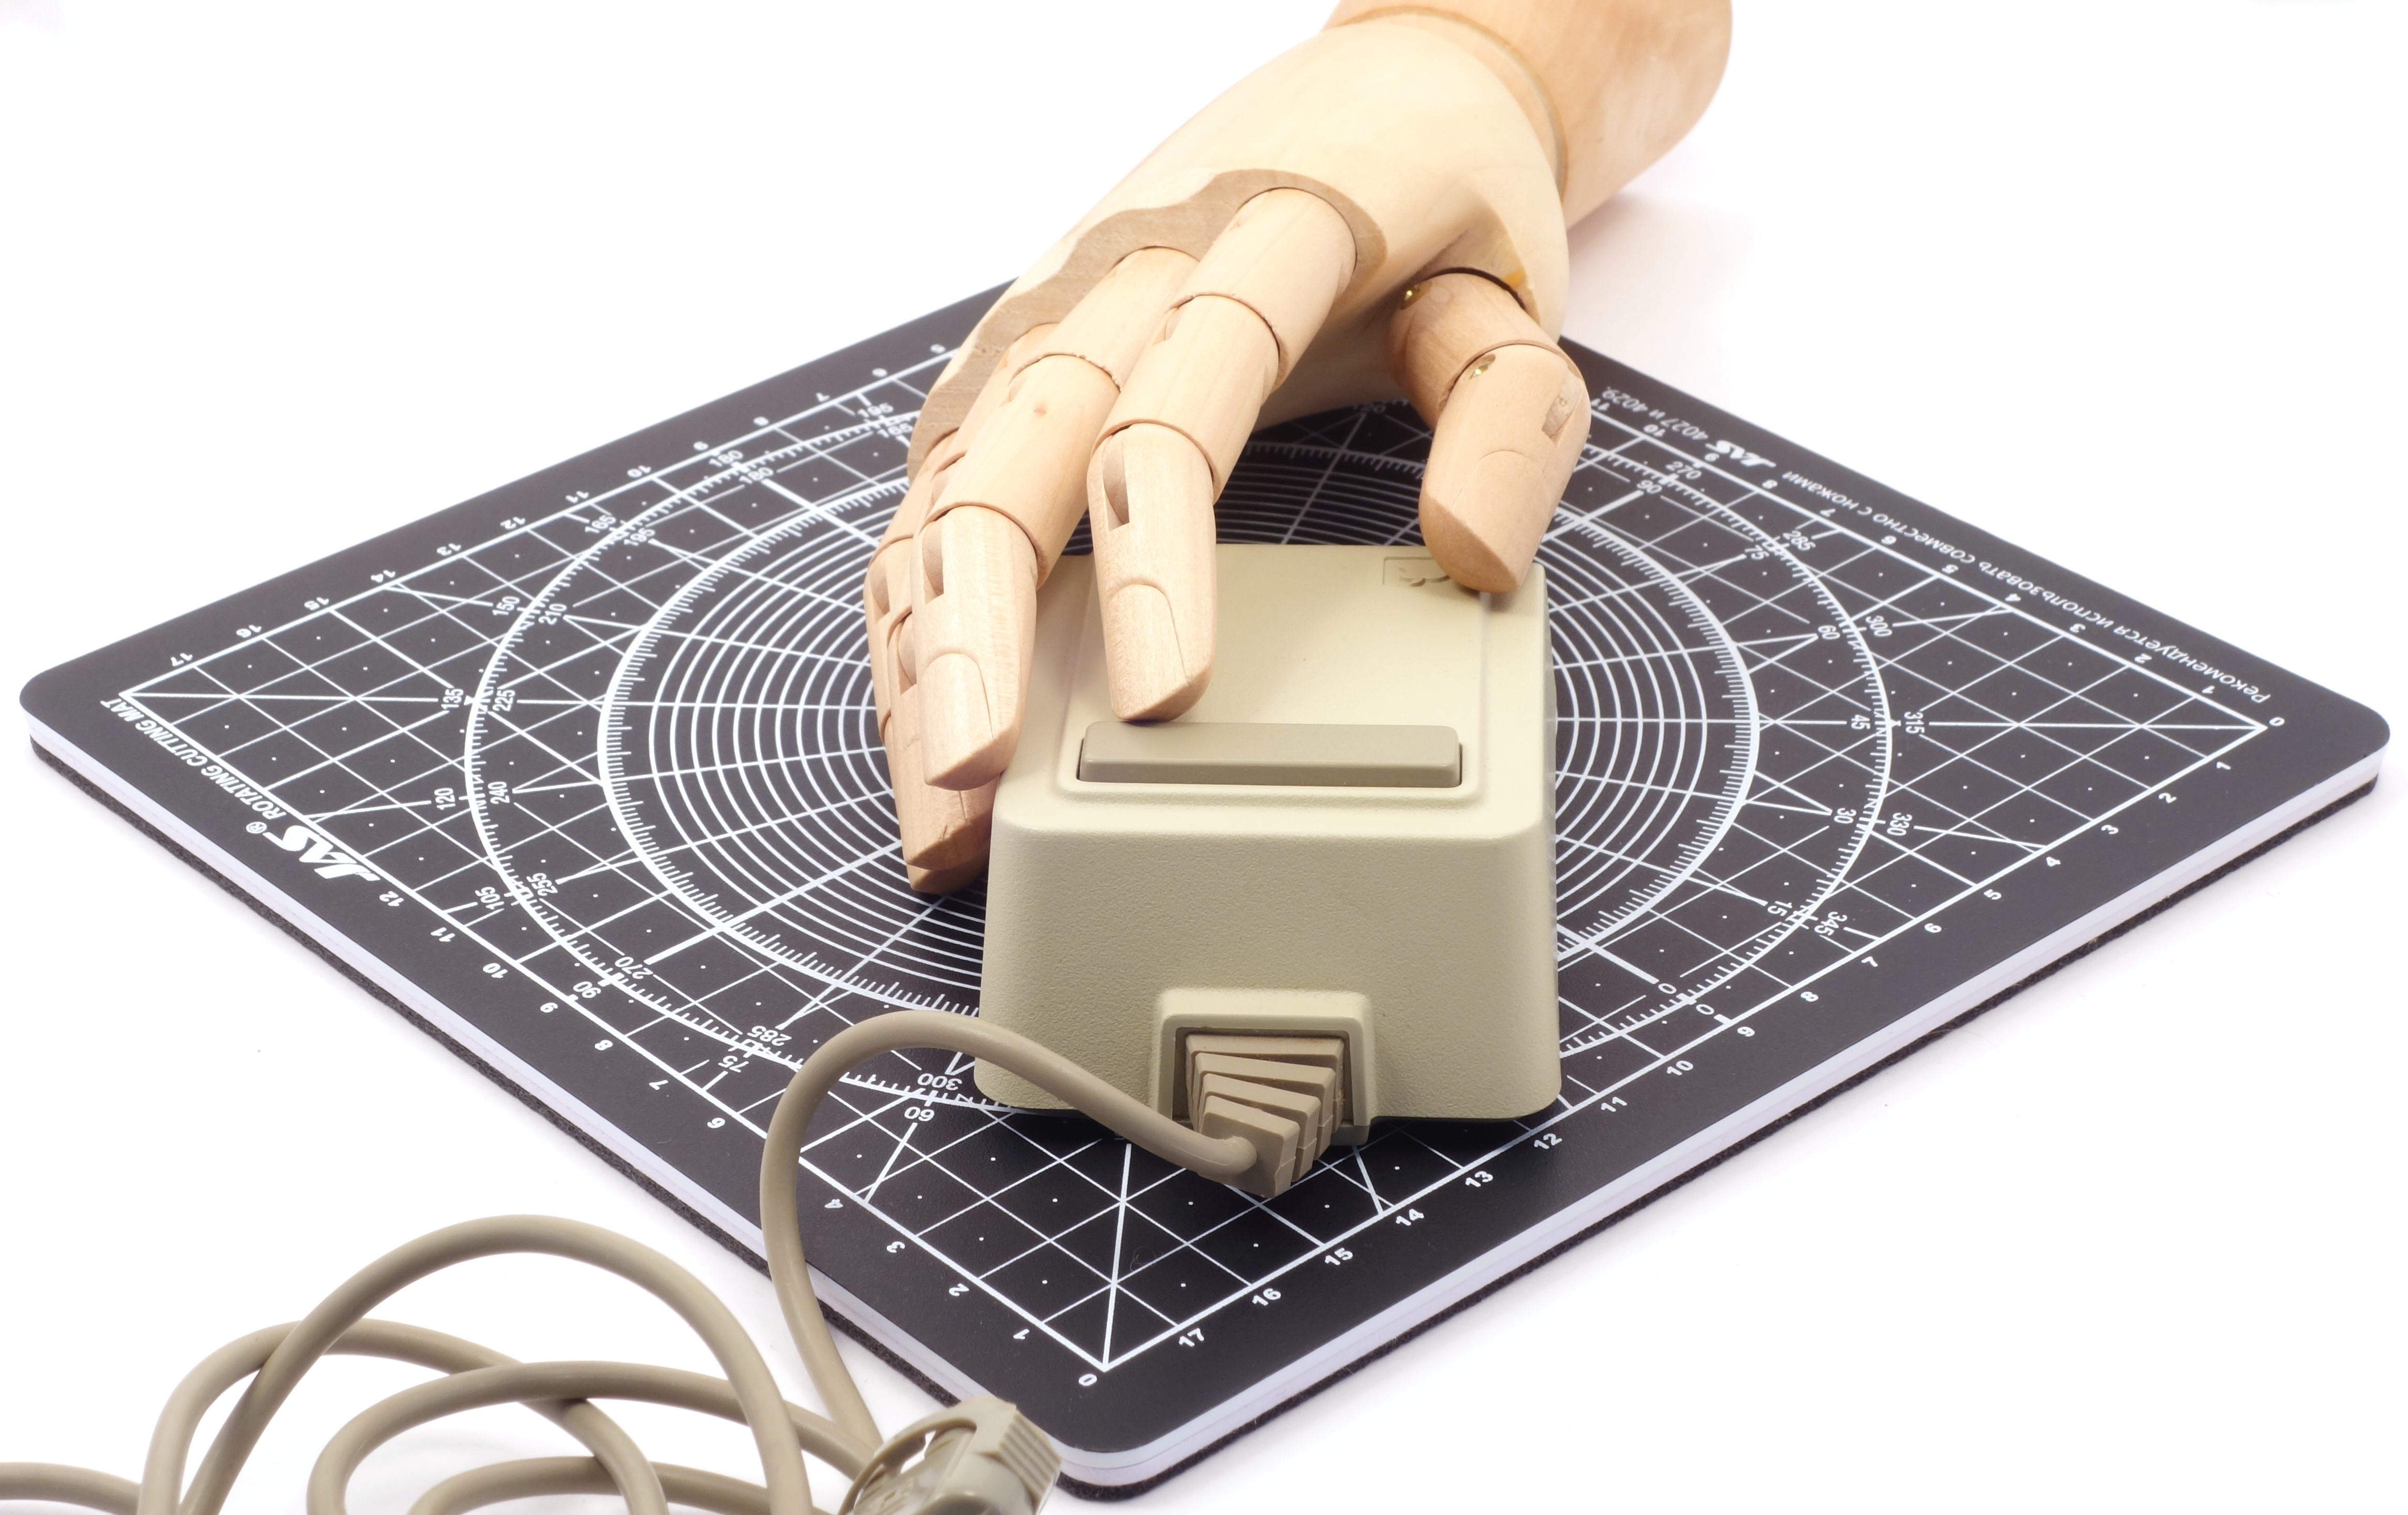
\includegraphics[scale=0.4]{1983_apple_lisa_mouse/appleruka_60.jpg}
    \caption{Apple Lisa mouse with a human hand model}
    \label{fig:AppleLisaHand}
\end{figure}

Mouse internals are shown on figure \ref{fig:AppleLisaInside}. A rather complex internal structure of the case with a significant number of partitions and additional supports can be noted. Having inherited the design of the optomechanical encoder practically unchanged, manufacturers of subsequent mice did step by step simplification of the case internal structure, reaching the almost hollow design of the device in the end of nineties.

 \begin{figure}[h]
    \centering
    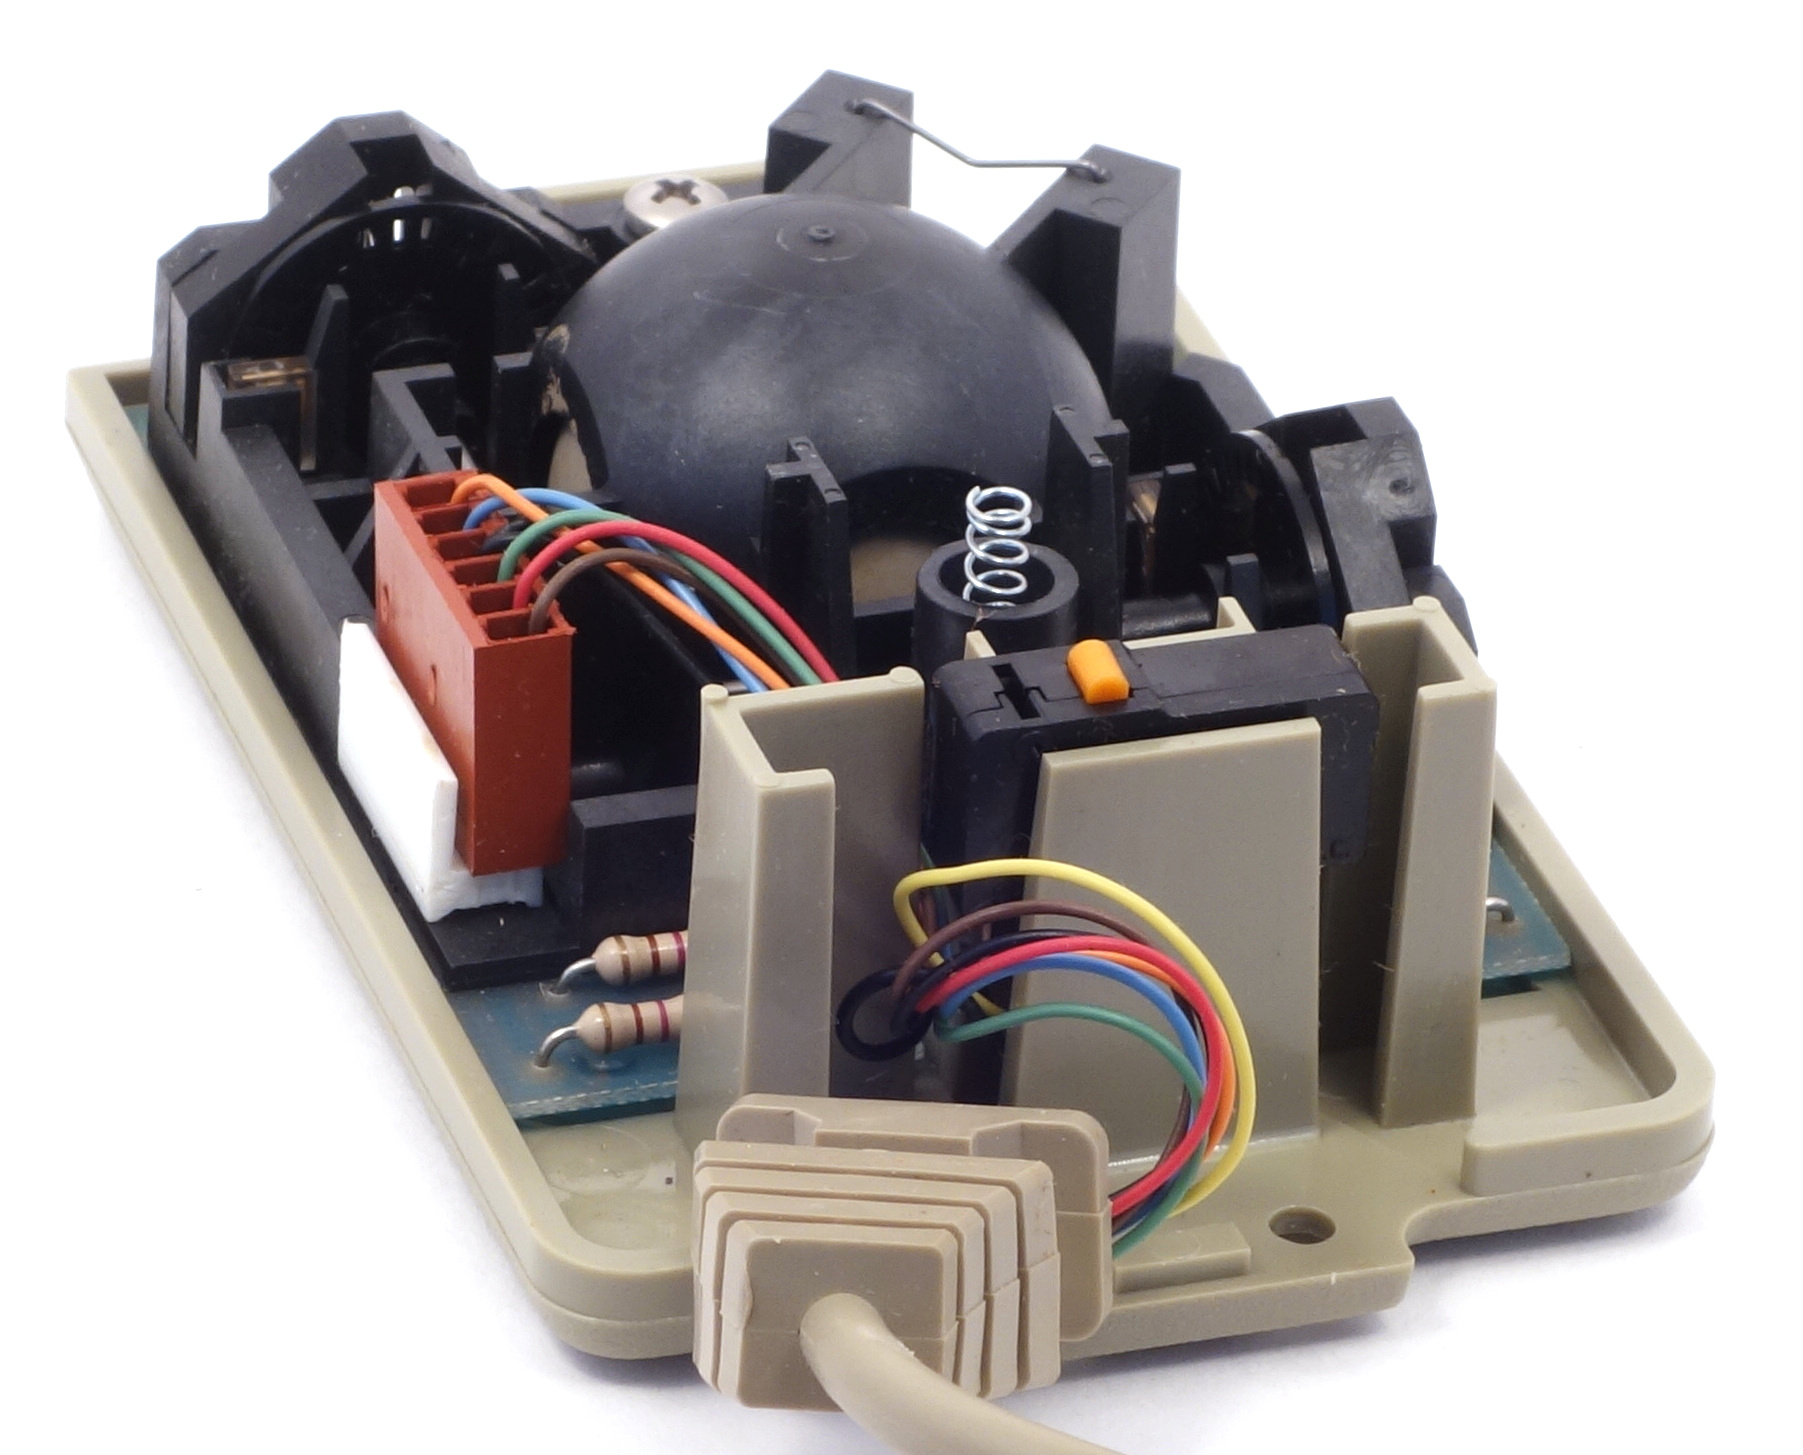
\includegraphics[scale=0.6]{1983_apple_lisa_mouse/appleraz_60.jpg}
    \caption{Apple Lisa mouse disassembled}
    \label{fig:AppleLisaInside}
\end{figure}

\begin{thebibliography}{9}
\bibitem {mouses} Apple Lisa I Mouse \url{https://www.oldmouse.com/mouse/apple/lisa.shtml}

\bibitem {ideo} Creating the First Usable Mouse \url{https://www.ideo.com/case-study/creating-the-first-usable-mouse}
\end{thebibliography}
\end{document}

\documentclass[11pt, a4paper]{article}
\usepackage{pdfpages}
\usepackage{parallel}
\usepackage[T2A]{fontenc}
\usepackage{ucs}
\usepackage[utf8x]{inputenc}
\usepackage[polish,english,russian]{babel}
\usepackage{hyperref}
\usepackage{rotating}
\usepackage[inner=2cm,top=1.8cm,outer=2cm,bottom=2.3cm,nohead]{geometry}
\usepackage{listings}
\usepackage{graphicx}
\usepackage{wrapfig}
\usepackage{longtable}
\usepackage{indentfirst}
\usepackage{array}
\usepackage{tikzsymbols}
\usepackage{soul}
\usepackage[ruled,vlined]{algorithm2e}
%\counterwithout{figure}{section} 

\usepackage{url}
\makeatletter
\g@addto@macro{\UrlBreaks}{\UrlOrds}
\makeatother

\newcolumntype{P}[1]{>{\raggedright\arraybackslash}p{#1}}
\frenchspacing
\usepackage{fixltx2e} %text sub- and superscripts
\usepackage{icomma} % коскі ў матэматычным рэжыме
\PreloadUnicodePage{4}

\newcommand{\longpage}{\enlargethispage{\baselineskip}}
\newcommand{\shortpage}{\enlargethispage{-\baselineskip}}

\def\switchlang#1{\expandafter\csname switchlang#1\endcsname}
\def\switchlangbe{
\let\saverefname=\refname%
\def\refname{Літаратура}%
\def\figurename{Іл.}%
}
\def\switchlangen{
\let\saverefname=\refname%
\def\refname{References}%
\def\figurename{Fig.}%
}
\def\switchlangru{
\let\saverefname=\refname%
\let\savefigurename=\figurename%
\def\refname{Литература}%
\def\figurename{Рис.}%
}

\hyphenation{admi-ni-stra-tive}
\hyphenation{ex-pe-ri-ence}
\hyphenation{fle-xi-bi-li-ty}
\hyphenation{Py-thon}
\hyphenation{ma-the-ma-ti-cal}
\hyphenation{re-ported}
\hyphenation{imp-le-menta-tions}
\hyphenation{pro-vides}
\hyphenation{en-gi-neering}
\hyphenation{com-pa-ti-bi-li-ty}
\hyphenation{im-pos-sible}
\hyphenation{desk-top}
\hyphenation{elec-tro-nic}
\hyphenation{com-pa-ny}
\hyphenation{de-ve-lop-ment}
\hyphenation{de-ve-loping}
\hyphenation{de-ve-lop}
\hyphenation{da-ta-ba-se}
\hyphenation{plat-forms}
\hyphenation{or-ga-ni-za-tion}
\hyphenation{pro-gramming}
\hyphenation{in-stru-ments}
\hyphenation{Li-nux}
\hyphenation{sour-ce}
\hyphenation{en-vi-ron-ment}
\hyphenation{Te-le-pathy}
\hyphenation{Li-nux-ov-ka}
\hyphenation{Open-BSD}
\hyphenation{Free-BSD}
\hyphenation{men-ti-on-ed}
\hyphenation{app-li-ca-tion}

\def\progref!#1!{\texttt{#1}}
\renewcommand{\arraystretch}{2} %Іначай формулы ў матрыцы зліпаюцца з лініямі
\usepackage{array}

\def\interview #1 (#2), #3, #4, #5\par{

\section[#1, #3, #4]{#1 -- #3, #4}
\def\qname{LVEE}
\def\aname{#1}
\def\q ##1\par{{\noindent \bf \qname: ##1 }\par}
\def\a{{\noindent \bf \aname: } \def\qname{L}\def\aname{#2}}
}

\def\interview* #1 (#2), #3, #4, #5\par{

\section*{#1\\{\small\rm #3, #4. #5}}
\ifx\ParallelWhichBox\undefined%
    \addcontentsline{toc}{section}{#1, #3, #4}%
\else%
\ifnum\ParallelWhichBox=0%
    \addcontentsline{toc}{section}{#1, #3, #4}%
\fi\fi%

\def\qname{LVEE}
\def\aname{#1}
\def\q ##1\par{{\noindent \bf \qname: ##1 }\par}
\def\a{{\noindent \bf \aname: } \def\qname{L}\def\aname{#2}}
}

\newcommand{\interviewfooter}[1]{
\vskip 1em
\noindent \textit{#1}
}


\begin{document}

\title{1983 "--- Hawley Mark II X063X Mouse}
\date{}
\maketitle

The Mark II X063X Mouse (figure \ref{fig:HawleyMarkIIPic}) was the first in-house development of the Hawley Mouse House \cite{hawley,mouses} by Jack Hawley, co-designer of the Xerox Alto computer mouse and co-author of the 1973 Xerox patent for mouse with two inclined wheels \cite{pat}.

\begin{figure}[h]
   \centering
    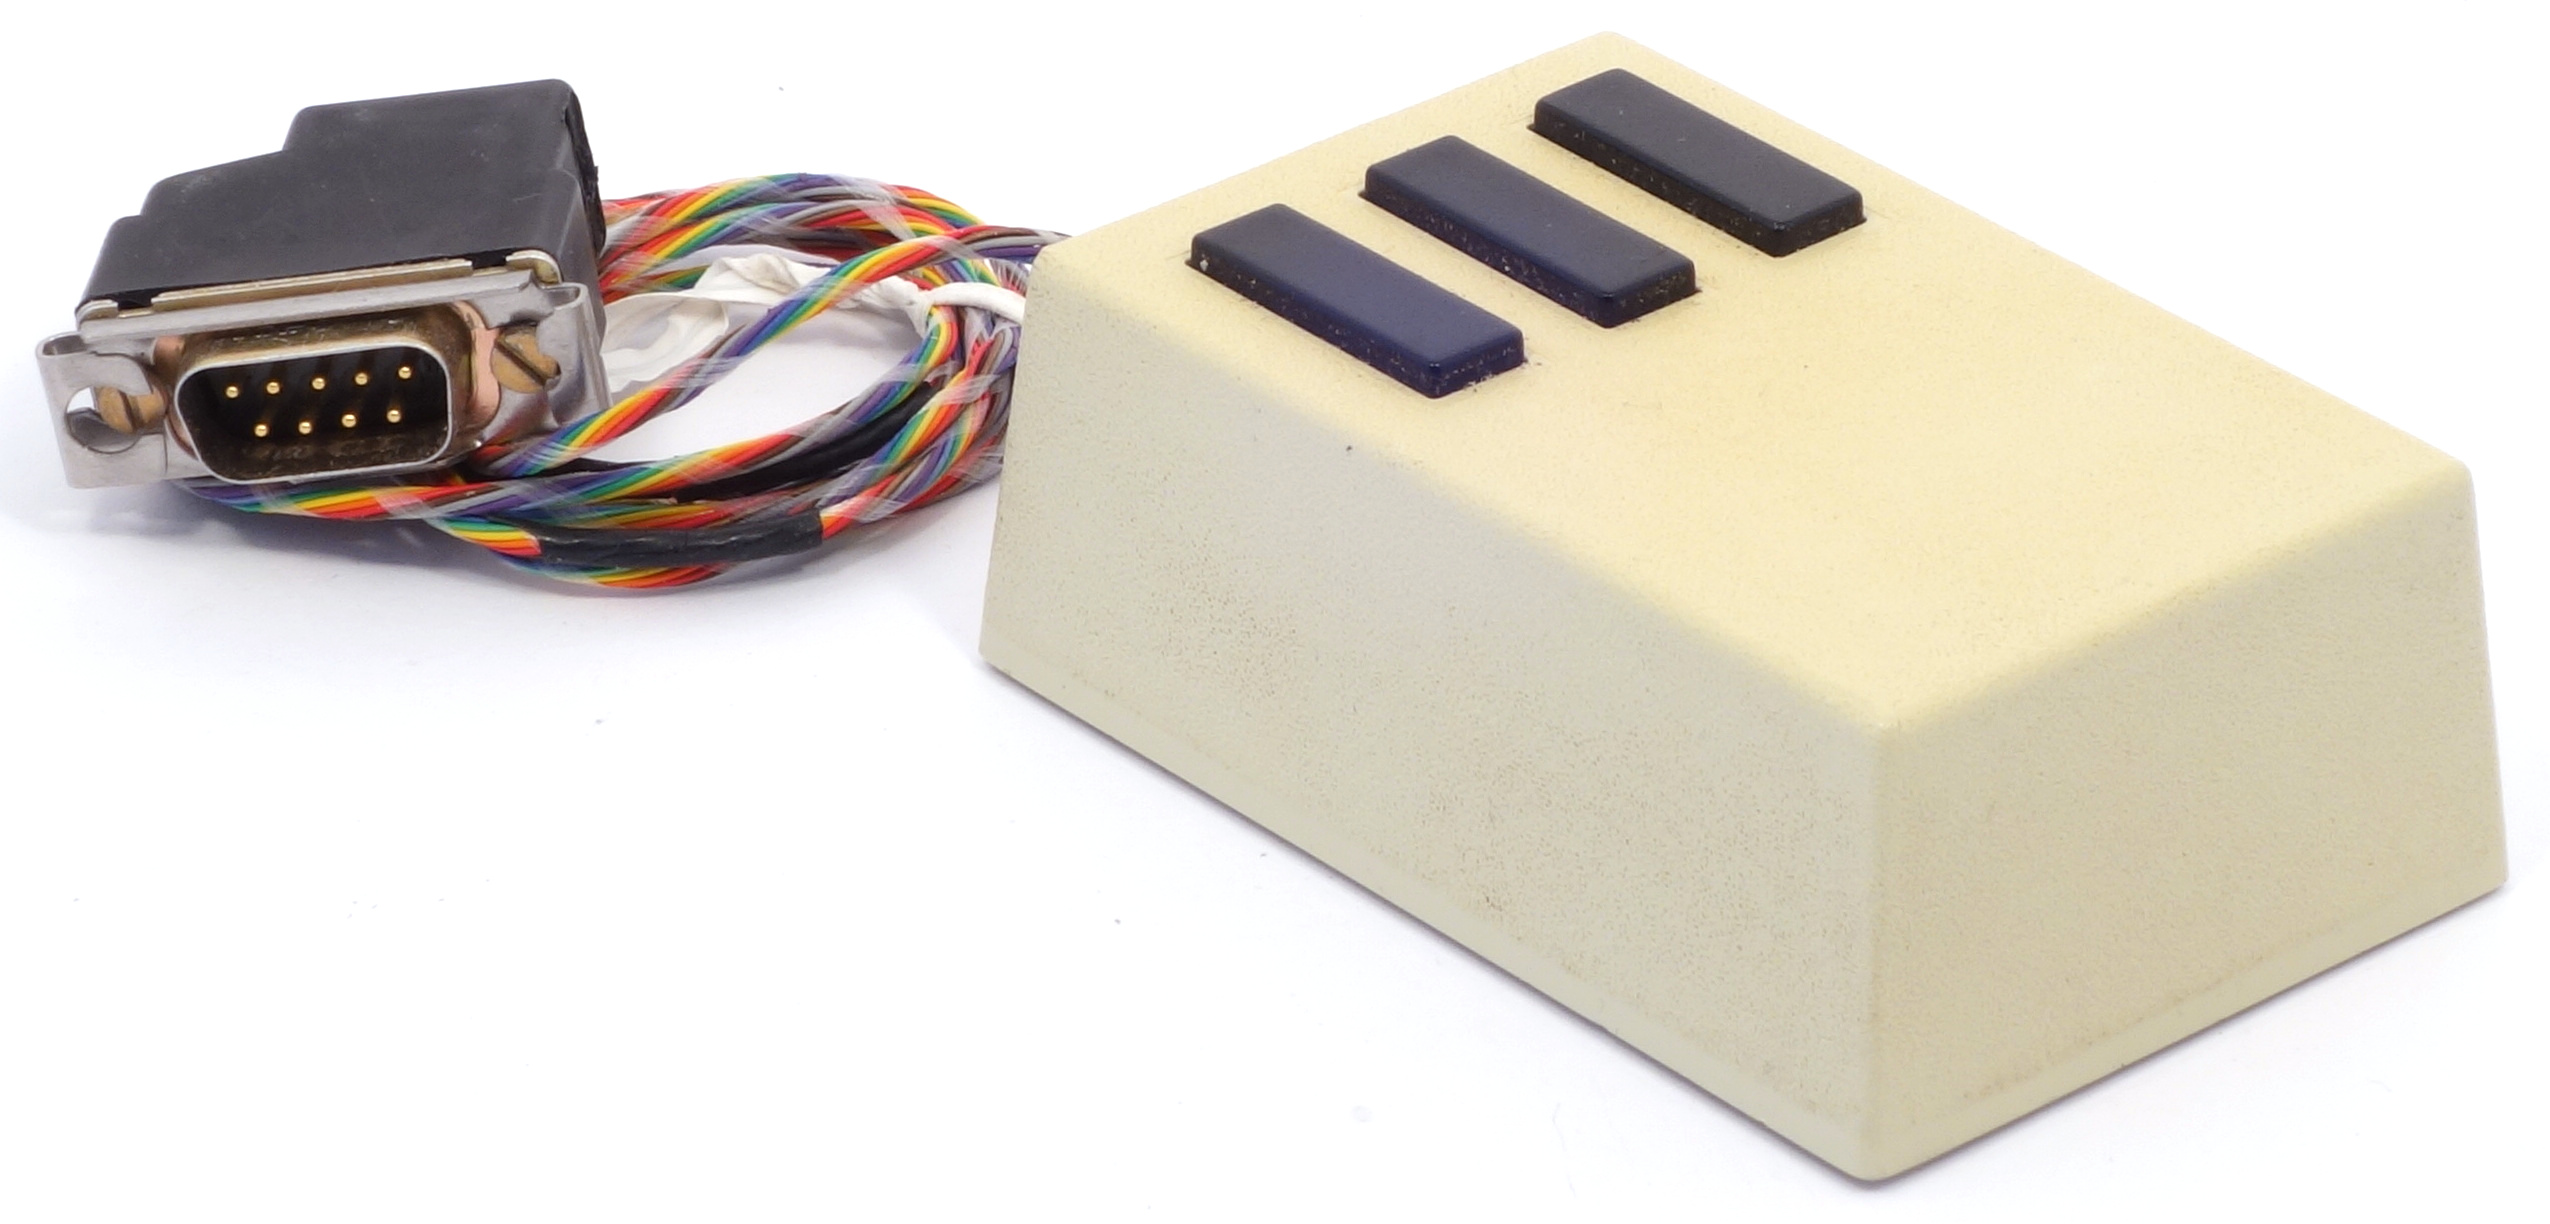
\includegraphics[scale=0.6]{1983_hawley_mark_ii/pic_60.jpg}
    \caption{Hawley Mark II X063X Mouse}
    \label{fig:HawleyMarkIIPic}
\end{figure}

The Mark II X063X mouse is made in an industrial design brought to an extreme degree: the body is an almost regular parallelepiped, on which there are three rectangular buttons with the most contrasting color in relation to the body (figure \ref{fig:HawleyMarkIITopAndBottom}). Obviously, the design was intended to emphasize the purpose of the mouse, aimed at engineers and users of various CAD systems (including solid modeling and architecture).

This item is beige with black buttons (on the cable you can see the remnants of black insulation, which has lost its elasticity over time and crumbled to pieces). The variant with the opposite combination of body and button colors was also common, and several more color options are known. The Hawley advertising gives an idea of the color combinations \cite{brochure}, but there is no information on how many color combinations from this promotional ad were actually implemented.

\begin{figure}[h]
    \centering
    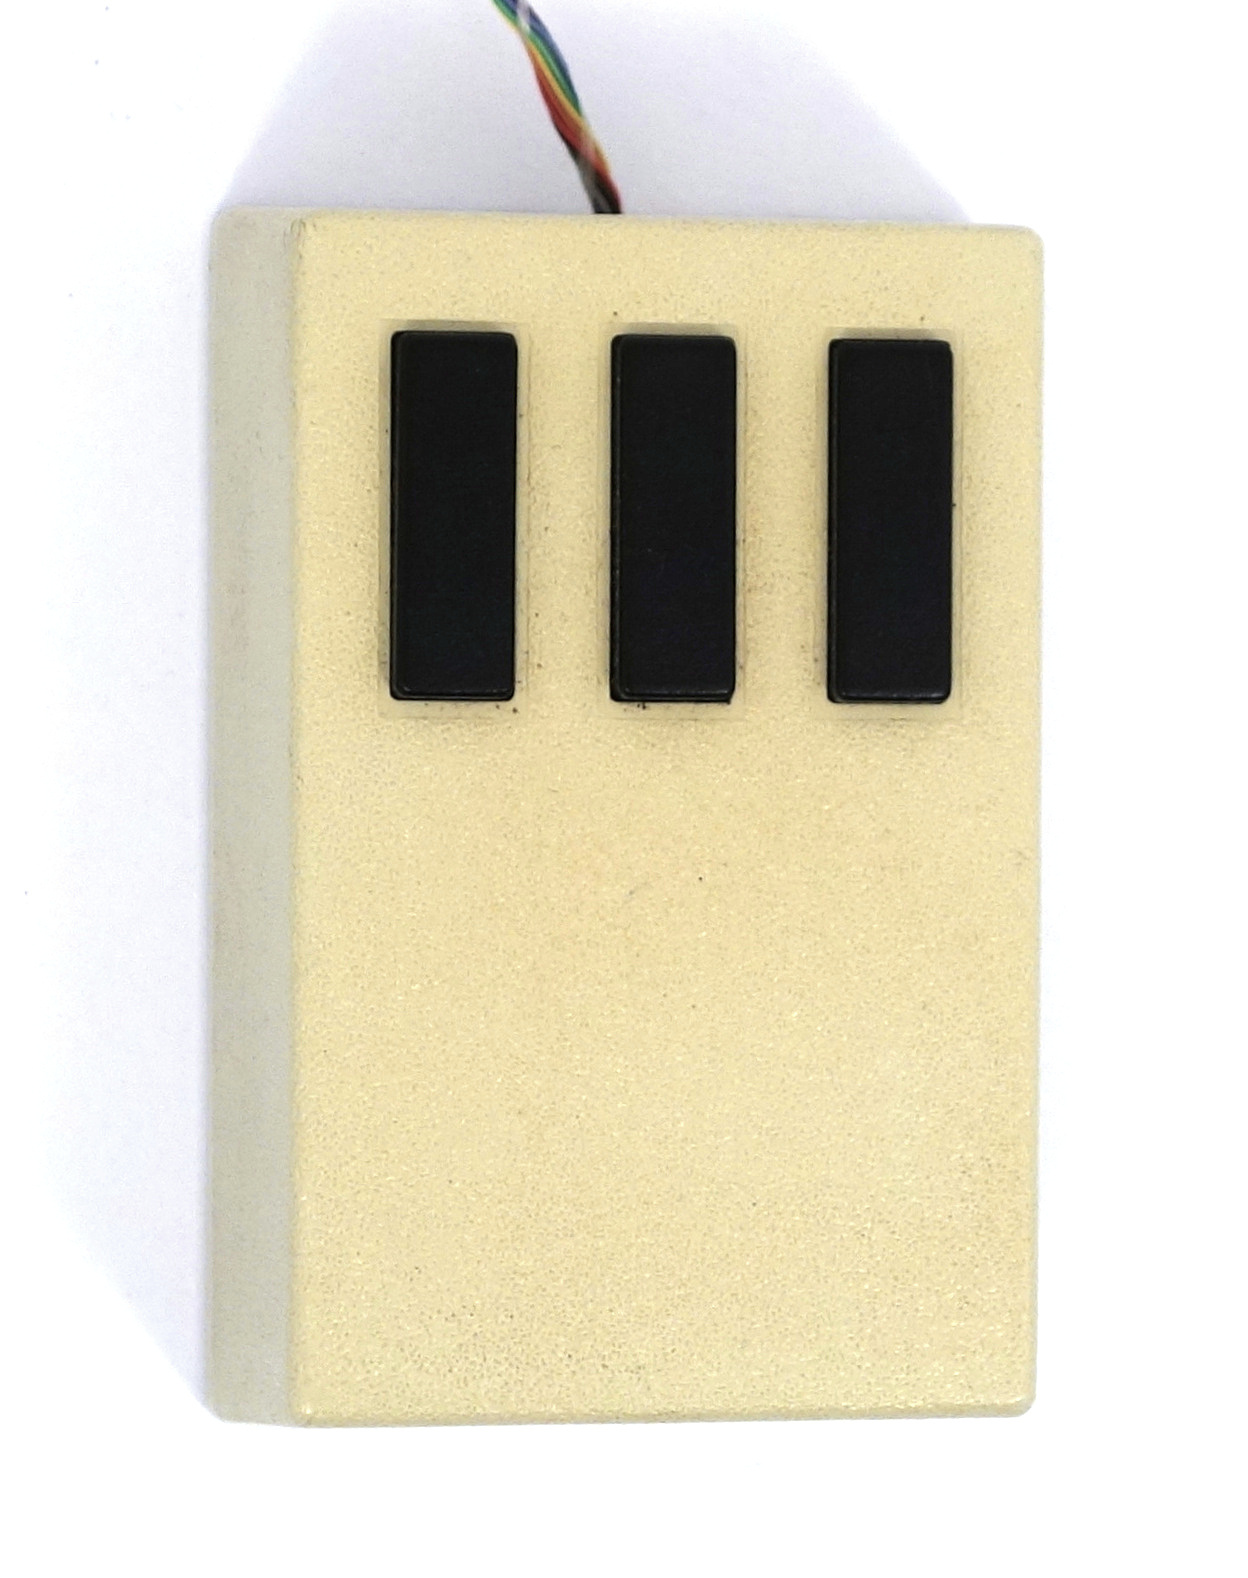
\includegraphics[scale=0.5]{1983_hawley_mark_ii/top_60.jpg}
    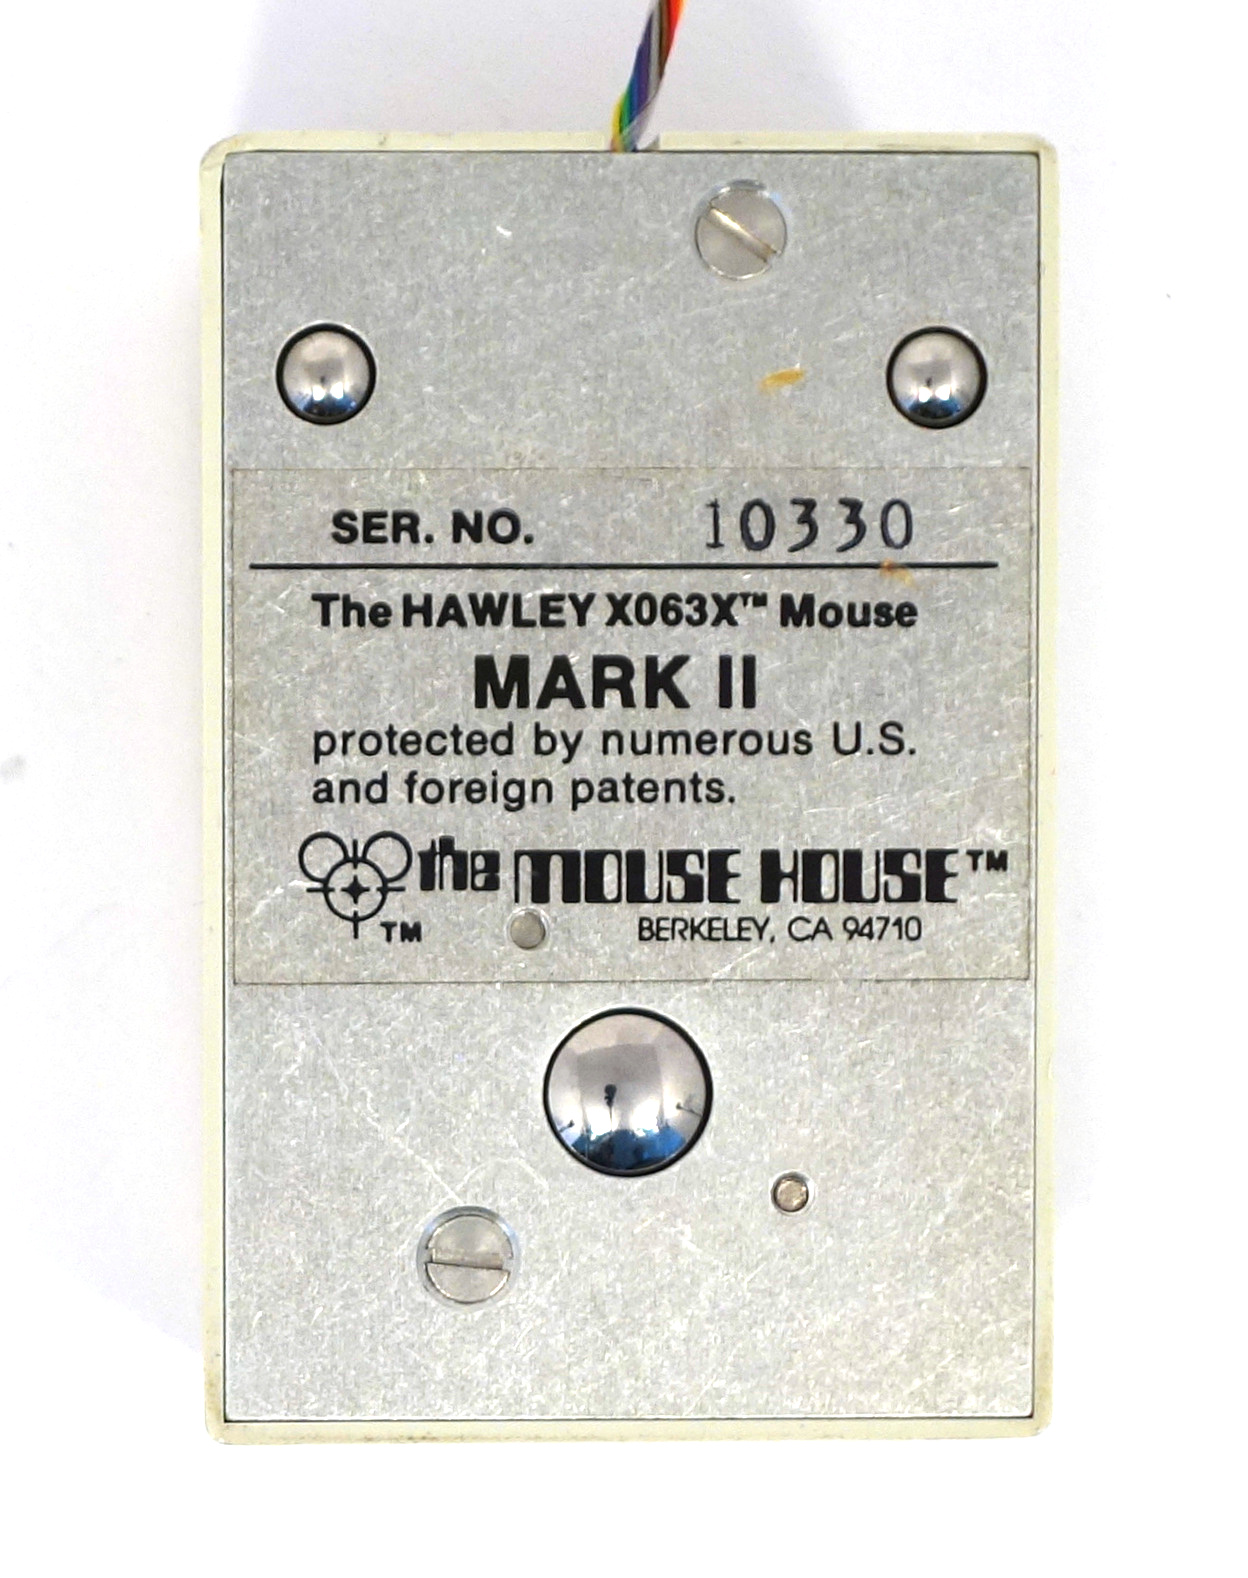
\includegraphics[scale=0.5]{1983_hawley_mark_ii/bottom_60.jpg}
    \caption{Hawley Mark II X063X Mouse, top and bottom views}
    \label{fig:HawleyMarkIITopAndBottom}
\end{figure}



Bottom side is entirely made of metal (figure \ref{fig:HawleyMarkIITopAndBottom}). Rotation is detected by a smooth steel ball in the center, while two smaller balls act as feet to minimize friction. A removable ring that allows you to remove the ball to remove collected debris is not yet provided in this model, so complete disassembly is necessary for cleaning.

\begin{figure}[h]
    \centering
    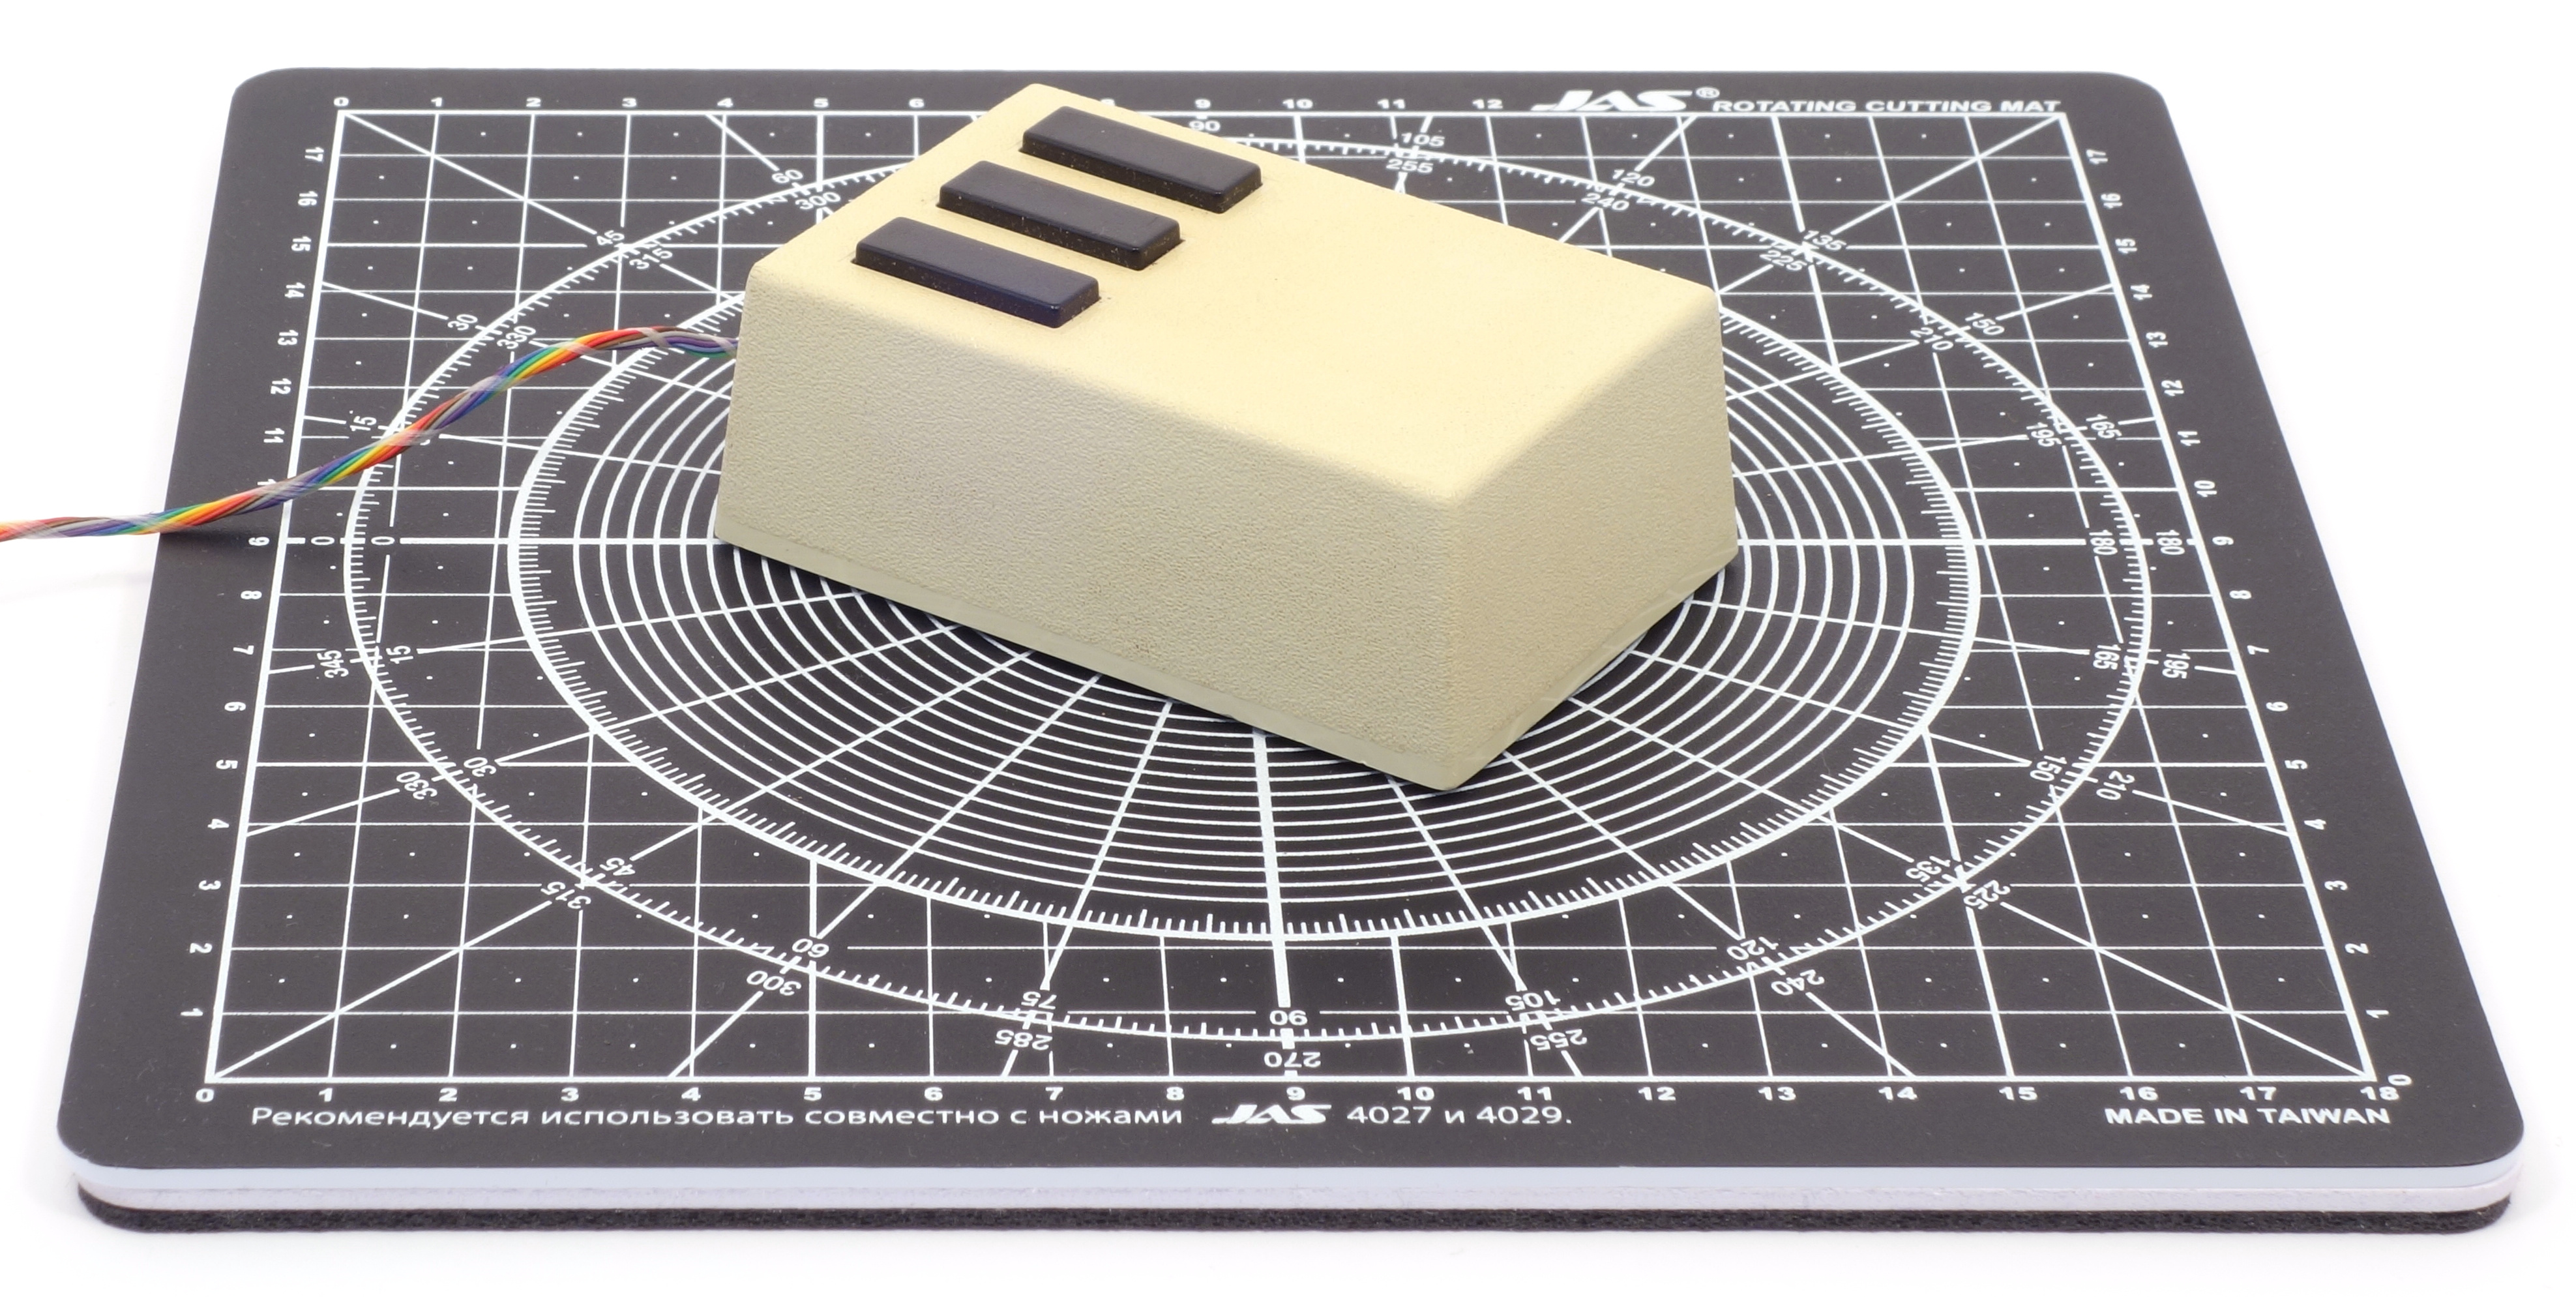
\includegraphics[scale=0.5]{1983_hawley_mark_ii/size_30.jpg}
    \caption{Hawley Mark II on a graduated pad with a grid step of 1~cm}
    \label{fig:HawleyMarkIISize}
\end{figure}

The mouse has a small size, typical for mice of the 1980s (figure \ref{fig:HawleyMarkIISize}). Obviously, this at least slightly reduces the negative impact of the body with orthogonal edges on ergonomics, since the hand can only lean on the body to a small extent (figure \ref{fig:HawleyMarkIIHand}).

\begin{figure}[h]
    \centering
    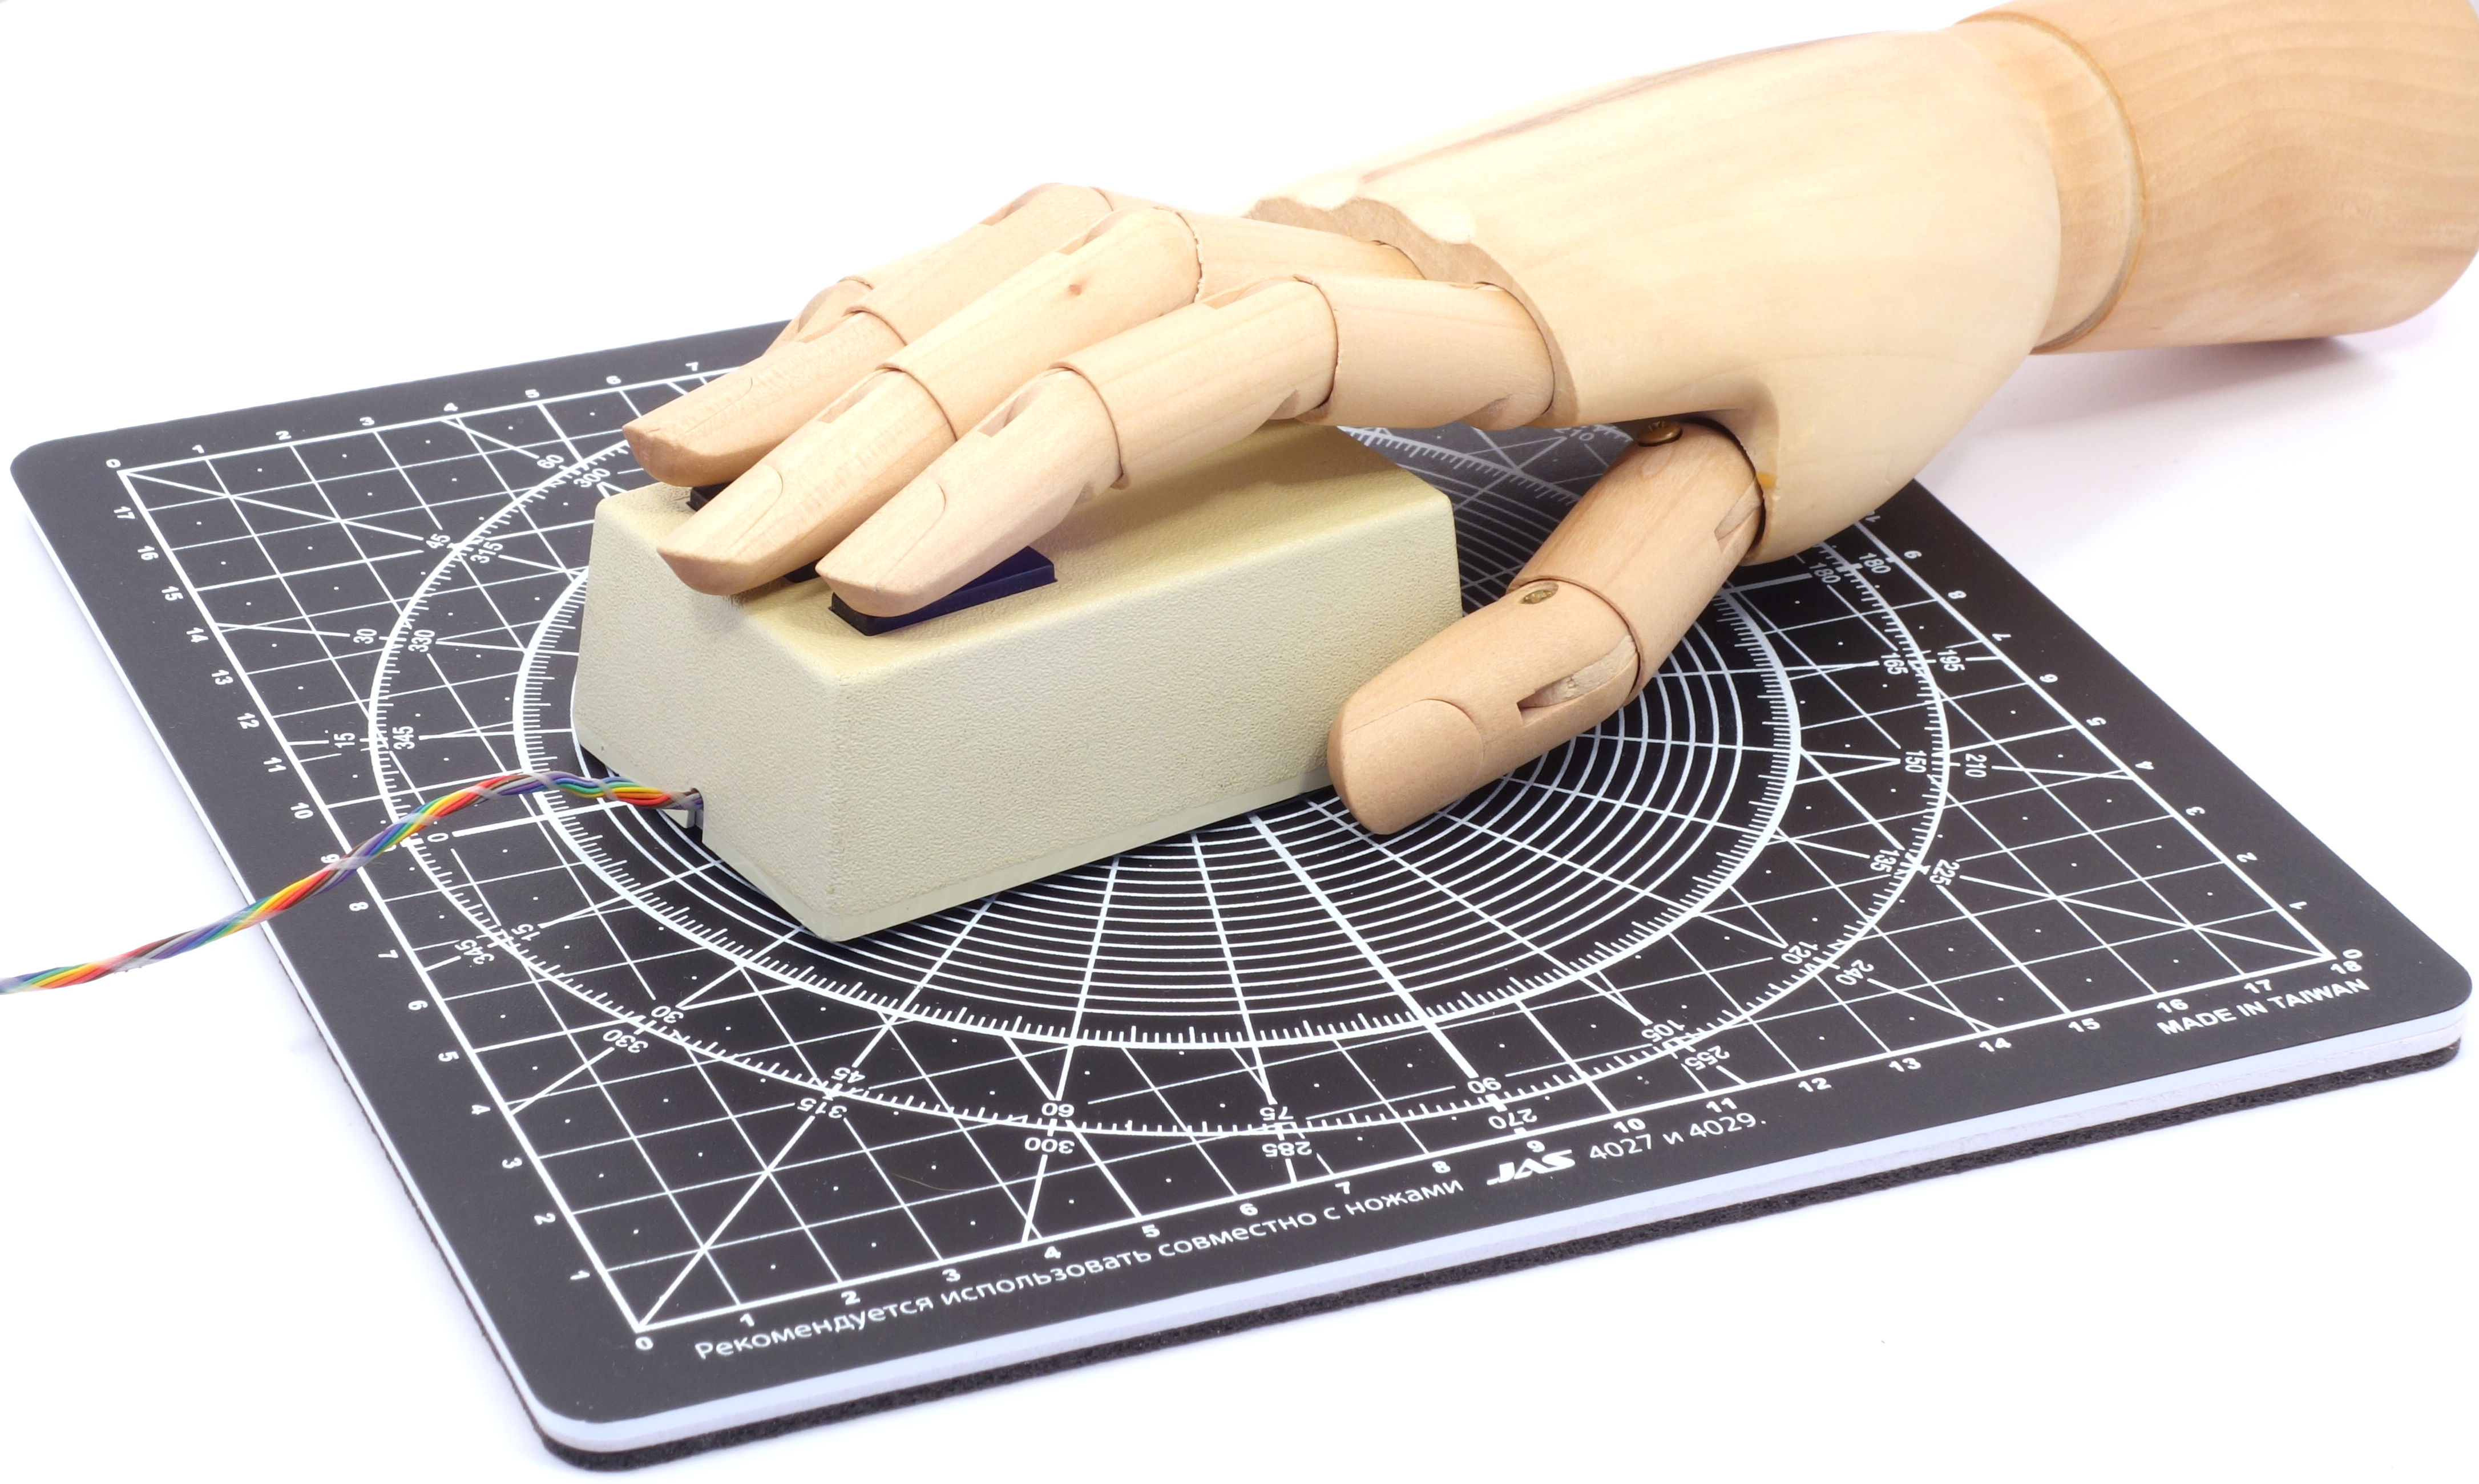
\includegraphics[scale=0.5]{1983_hawley_mark_ii/hand_60.jpg}
    \caption{Hawley Mark II with a human hand model}
    \label{fig:HawleyMarkIIHand}
\end{figure}

Mouse internals are shown on figure \ref{fig:HawleyMarkIIInside}. The removable solid protection of the ball is worthy of mention: it requires additional disassembly operations to remove garbage. In this mouse, contact encoders (with four contacts for greater reliability) are used, which are based on a metal contact drum instead of the more common disk in subsequent models.

 \begin{figure}[h]
    \centering
    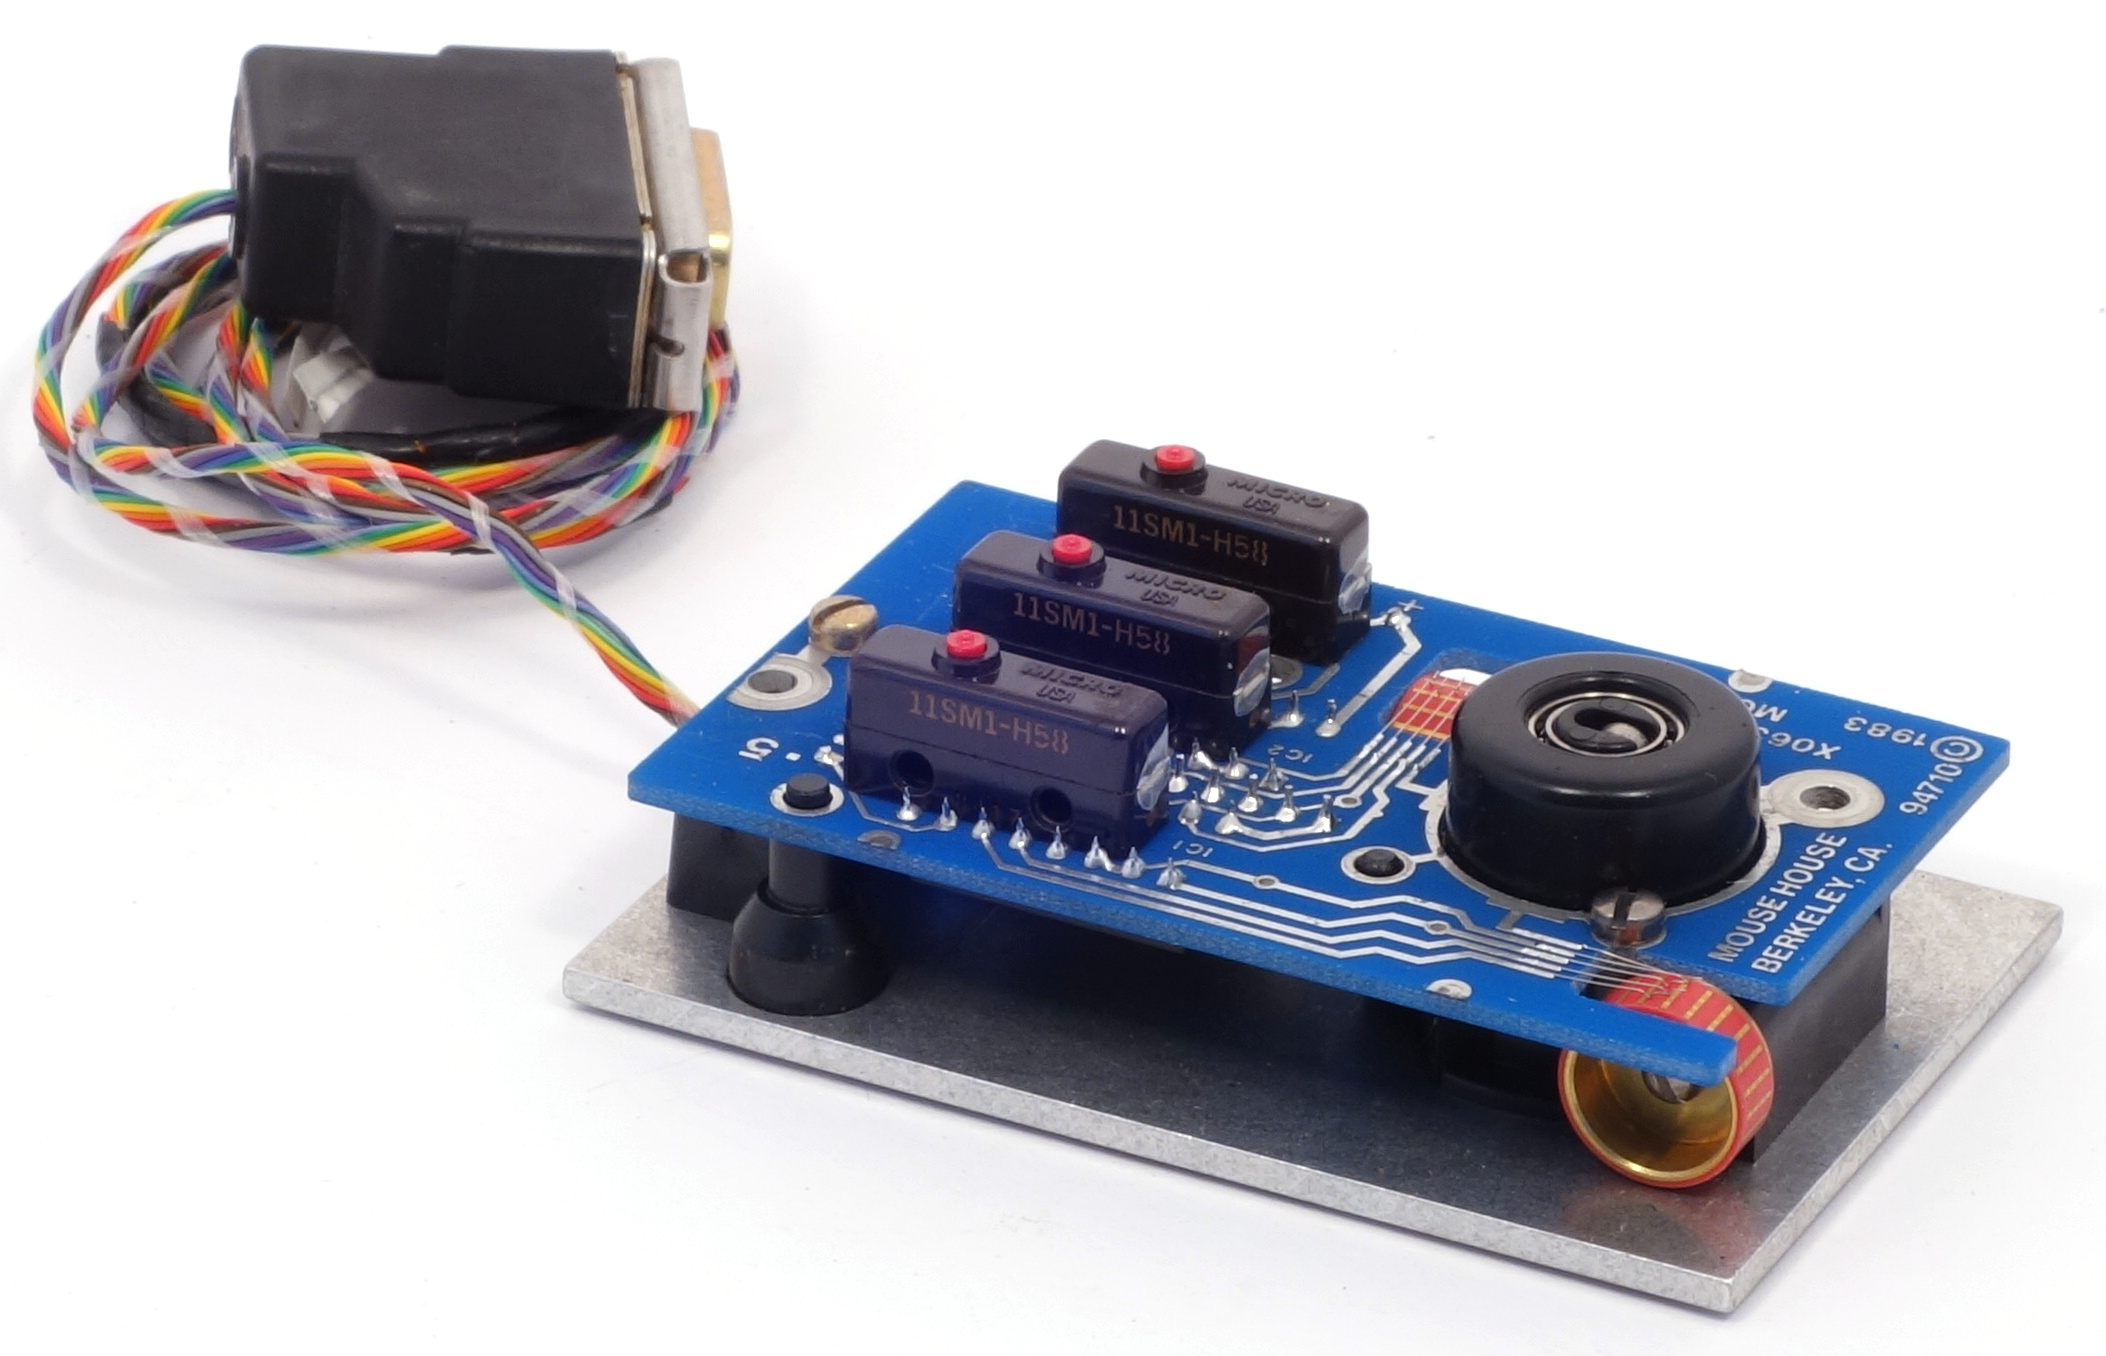
\includegraphics[scale=0.8]{1983_hawley_mark_ii/inside_60.jpg}
    \caption{Hawley Mark II disassembled}
    \label{fig:HawleyMarkIIInside}
\end{figure}

\begin{thebibliography}{9}
\bibitem{hawley} Hawley Mouse House \url{https://oldmouse.com/mouse/hawley/}

\bibitem{mouses} Hawley Mark II X063X Mouses \url{https://oldmouse.com/mouse/hawley/X063X.shtml}

\bibitem{pat} Transducer for a display-oriented pointing device \url{https://patents.google.com/patent/US3892963A/en}

\bibitem{brochure} Mouse House MK II Brochure \url{https://www.microsoft.com/buxtoncollection/a/pdf/Mouse%20House%20MK%20II%20Brochure.pdf}
\end{thebibliography}
\end{document}

\documentclass[11pt, a4paper]{article}
\usepackage{pdfpages}
\usepackage{parallel}
\usepackage[T2A]{fontenc}
\usepackage{ucs}
\usepackage[utf8x]{inputenc}
\usepackage[polish,english,russian]{babel}
\usepackage{hyperref}
\usepackage{rotating}
\usepackage[inner=2cm,top=1.8cm,outer=2cm,bottom=2.3cm,nohead]{geometry}
\usepackage{listings}
\usepackage{graphicx}
\usepackage{wrapfig}
\usepackage{longtable}
\usepackage{indentfirst}
\usepackage{array}
\usepackage{tikzsymbols}
\usepackage{soul}
\usepackage[ruled,vlined]{algorithm2e}
%\counterwithout{figure}{section} 

\usepackage{url}
\makeatletter
\g@addto@macro{\UrlBreaks}{\UrlOrds}
\makeatother

\newcolumntype{P}[1]{>{\raggedright\arraybackslash}p{#1}}
\frenchspacing
\usepackage{fixltx2e} %text sub- and superscripts
\usepackage{icomma} % коскі ў матэматычным рэжыме
\PreloadUnicodePage{4}

\newcommand{\longpage}{\enlargethispage{\baselineskip}}
\newcommand{\shortpage}{\enlargethispage{-\baselineskip}}

\def\switchlang#1{\expandafter\csname switchlang#1\endcsname}
\def\switchlangbe{
\let\saverefname=\refname%
\def\refname{Літаратура}%
\def\figurename{Іл.}%
}
\def\switchlangen{
\let\saverefname=\refname%
\def\refname{References}%
\def\figurename{Fig.}%
}
\def\switchlangru{
\let\saverefname=\refname%
\let\savefigurename=\figurename%
\def\refname{Литература}%
\def\figurename{Рис.}%
}

\hyphenation{admi-ni-stra-tive}
\hyphenation{ex-pe-ri-ence}
\hyphenation{fle-xi-bi-li-ty}
\hyphenation{Py-thon}
\hyphenation{ma-the-ma-ti-cal}
\hyphenation{re-ported}
\hyphenation{imp-le-menta-tions}
\hyphenation{pro-vides}
\hyphenation{en-gi-neering}
\hyphenation{com-pa-ti-bi-li-ty}
\hyphenation{im-pos-sible}
\hyphenation{desk-top}
\hyphenation{elec-tro-nic}
\hyphenation{com-pa-ny}
\hyphenation{de-ve-lop-ment}
\hyphenation{de-ve-loping}
\hyphenation{de-ve-lop}
\hyphenation{da-ta-ba-se}
\hyphenation{plat-forms}
\hyphenation{or-ga-ni-za-tion}
\hyphenation{pro-gramming}
\hyphenation{in-stru-ments}
\hyphenation{Li-nux}
\hyphenation{sour-ce}
\hyphenation{en-vi-ron-ment}
\hyphenation{Te-le-pathy}
\hyphenation{Li-nux-ov-ka}
\hyphenation{Open-BSD}
\hyphenation{Free-BSD}
\hyphenation{men-ti-on-ed}
\hyphenation{app-li-ca-tion}

\def\progref!#1!{\texttt{#1}}
\renewcommand{\arraystretch}{2} %Іначай формулы ў матрыцы зліпаюцца з лініямі
\usepackage{array}

\def\interview #1 (#2), #3, #4, #5\par{

\section[#1, #3, #4]{#1 -- #3, #4}
\def\qname{LVEE}
\def\aname{#1}
\def\q ##1\par{{\noindent \bf \qname: ##1 }\par}
\def\a{{\noindent \bf \aname: } \def\qname{L}\def\aname{#2}}
}

\def\interview* #1 (#2), #3, #4, #5\par{

\section*{#1\\{\small\rm #3, #4. #5}}
\ifx\ParallelWhichBox\undefined%
    \addcontentsline{toc}{section}{#1, #3, #4}%
\else%
\ifnum\ParallelWhichBox=0%
    \addcontentsline{toc}{section}{#1, #3, #4}%
\fi\fi%

\def\qname{LVEE}
\def\aname{#1}
\def\q ##1\par{{\noindent \bf \qname: ##1 }\par}
\def\a{{\noindent \bf \aname: } \def\qname{L}\def\aname{#2}}
}

\newcommand{\interviewfooter}[1]{
\vskip 1em
\noindent \textit{#1}
}

\switchlang{en}
\begin{document}

\title{1983 "--- DEC VS10X-EA Mouse}
\date{}
\maketitle
\selectlanguage{english}
The DEC VS10X-EA mouse (fig. \ref{fig:DecVS10XPic}) was released in 1983, and it is heavily based on the Hawley Mouse House \cite{hawley,mouses} by Jack Hawley, co-designer of the Xerox Alto computer mouse and one of the authors 1973 Xerox patent for a two-wheel tilt mouse \cite{pat}. In fact, the DEC VS10X-EA is a modification of the Hawley Mark II X063X Mouse of the same year. Comparison of the two mice reveals no technical differences except the shape of the case and connector. The mouse was supplied with the DEC VAXstation 100 graphical terminals \cite{reddit} used in creation of the X Windows System, a graphical windowing system for Unix-like OS.

\begin{figure}[h]
   \centering
    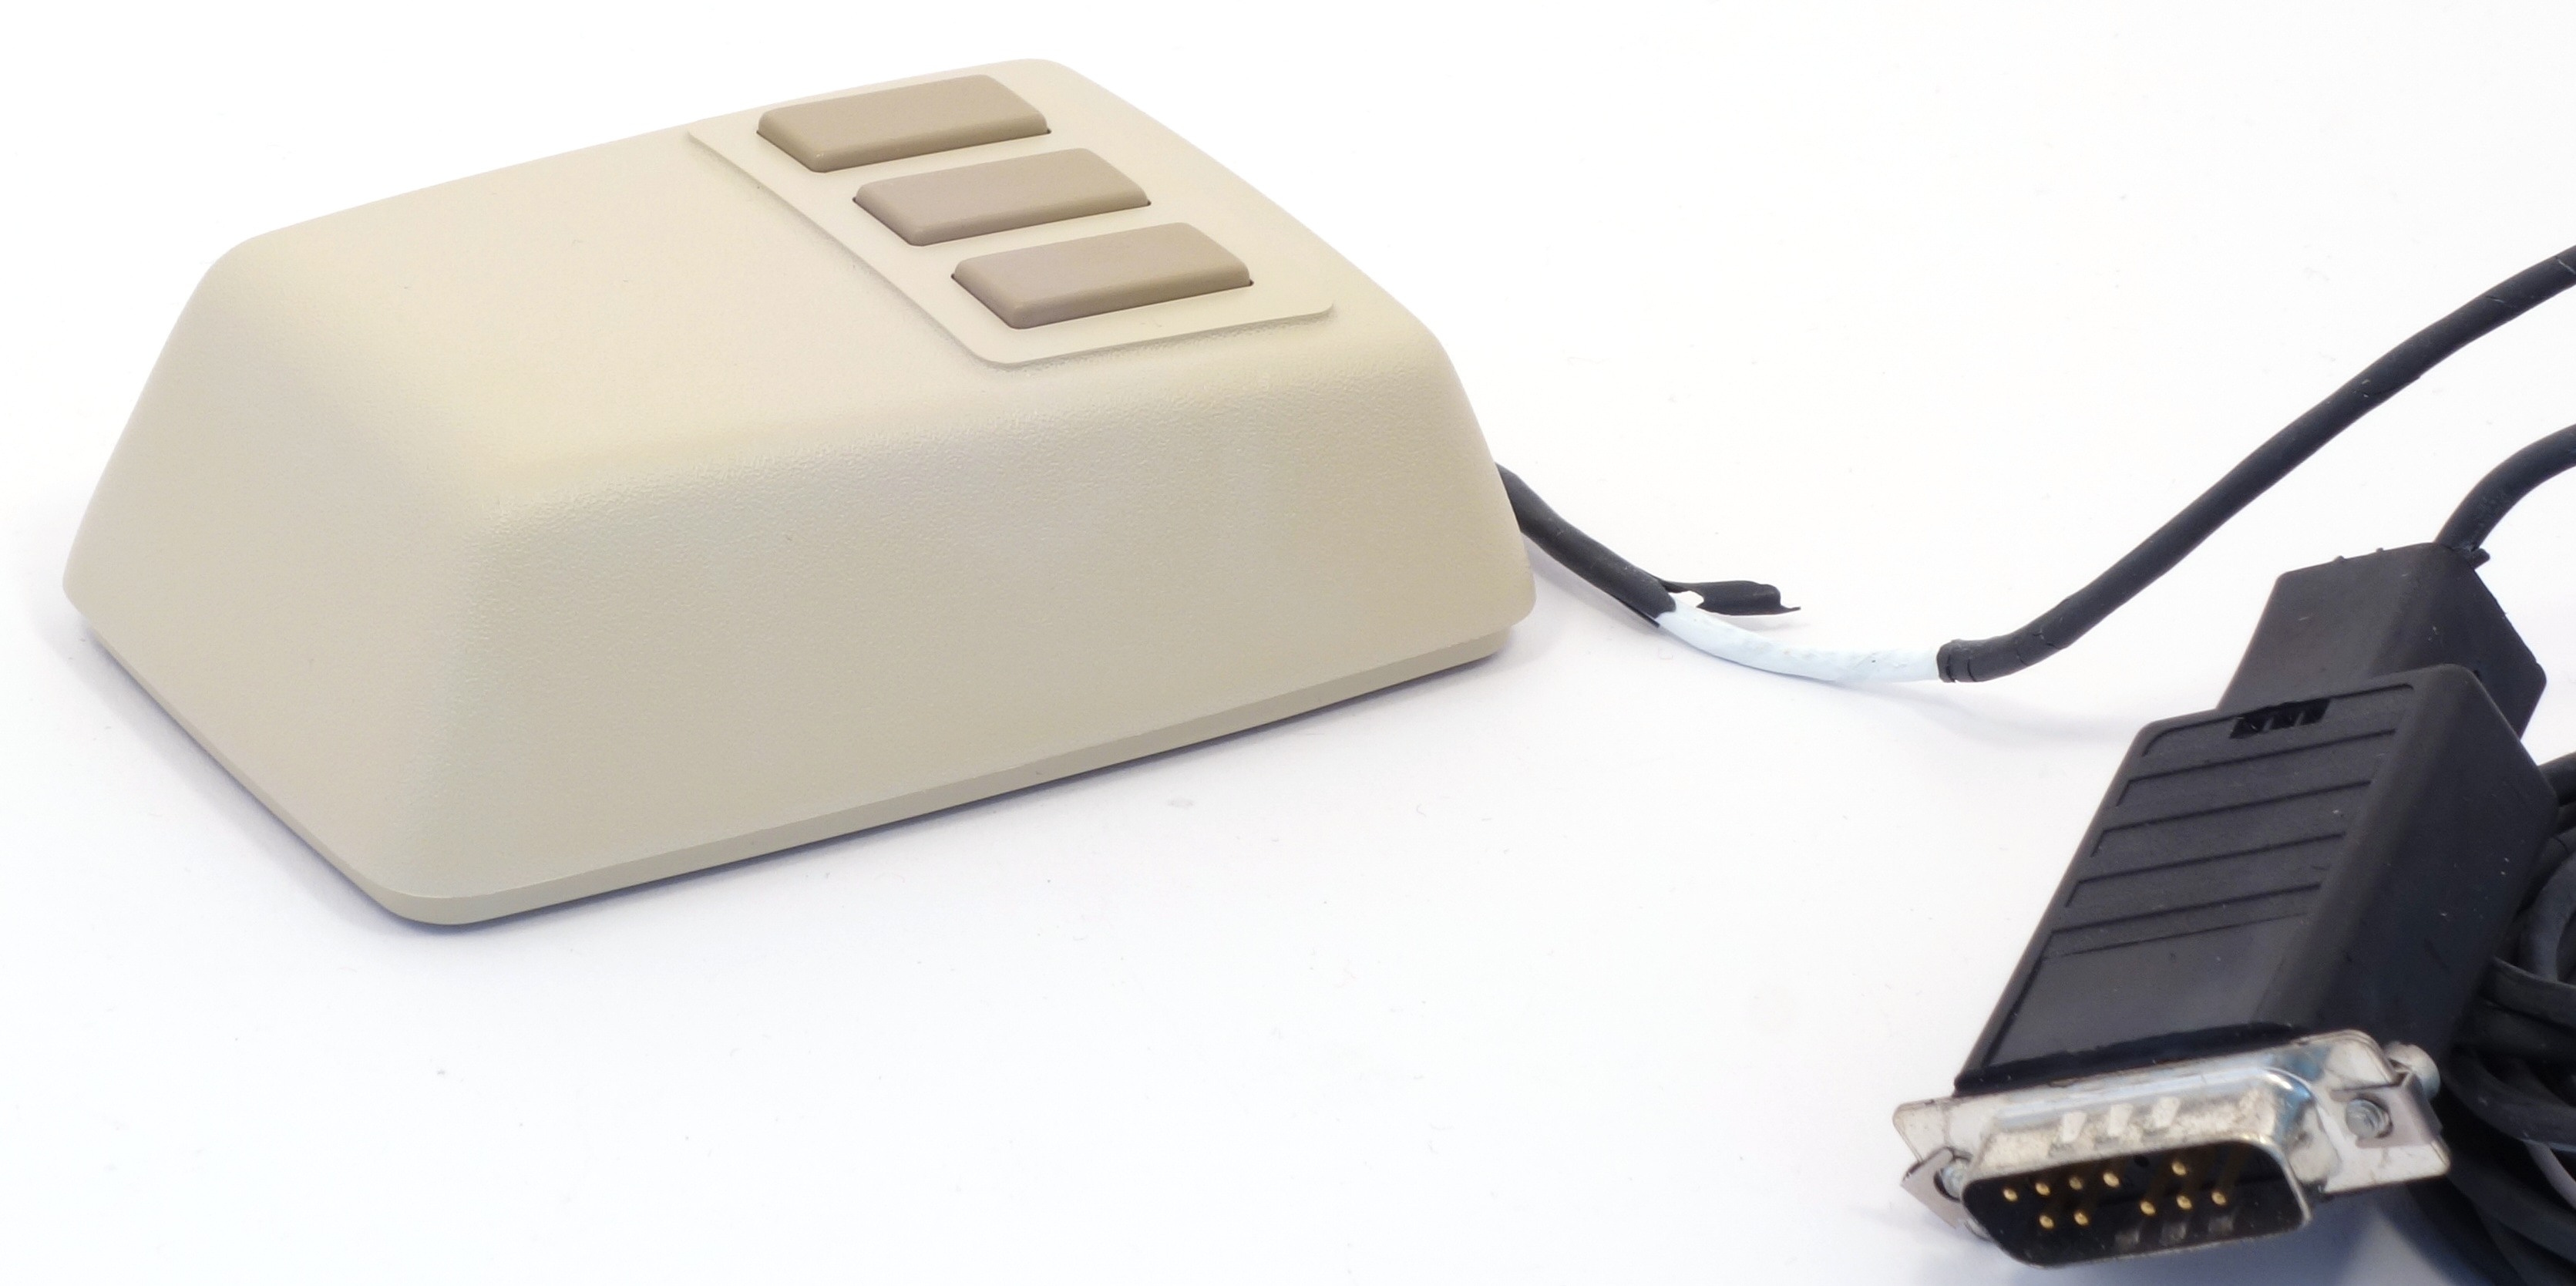
\includegraphics[scale=0.6]{1983_dec_vs10x_ea_mouse/pic_30.jpg}
    \caption{DEC VS10X-EA Mouse}
    \label{fig:DecVS10XPic}
\end{figure}

By contrast with the prototype mouse’s body (a parallelepiped with three rectangular buttons), the body of DEC VS10X-EA has a smoother shape with a substantially inclined sides and smooth transitions between the faces. Both mice have same internals, so the smoother shape is achieved at the cost of the increased size, and Hawley mouse’s rectangle is still easily seen on the bottom (fig. \ref{fig:DecVS10XTopAndBottom}). Obviously, such improvements had a positive effect on the ergonomics of the device.

\begin{figure}[h]
    \centering
    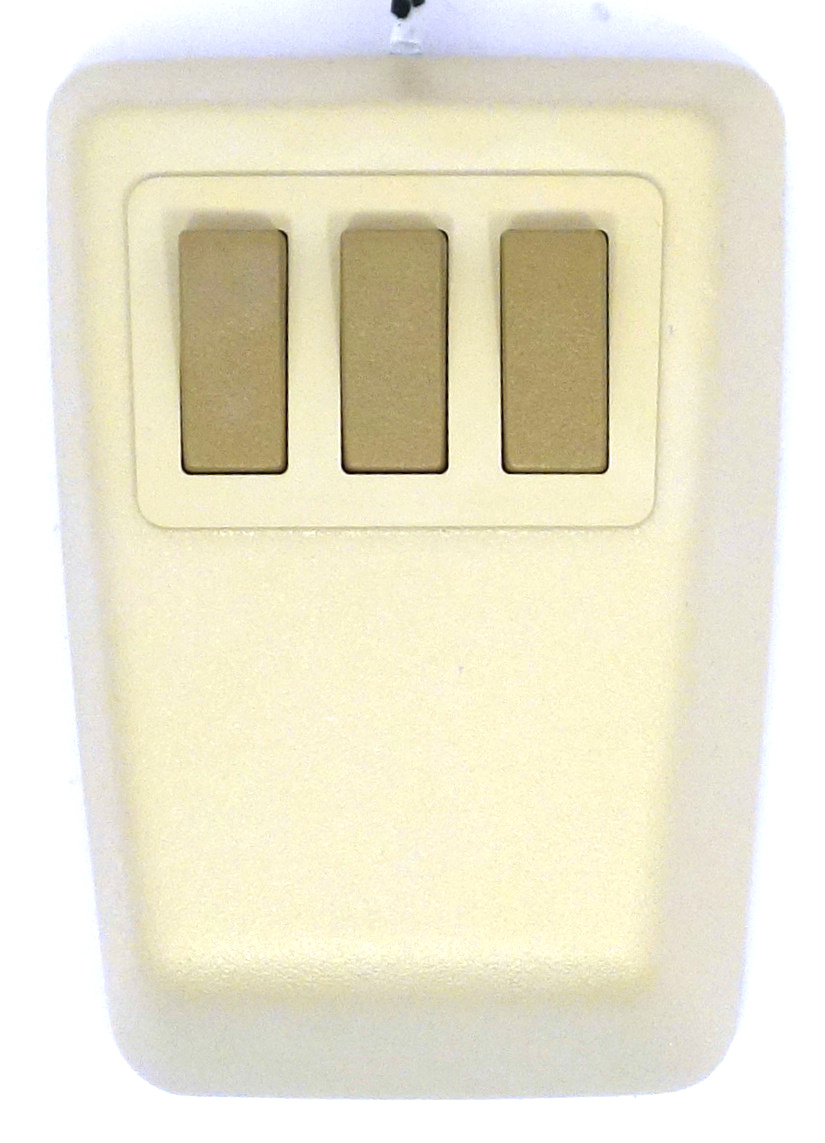
\includegraphics[scale=0.55]{1983_dec_vs10x_ea_mouse/top_60.jpg}
    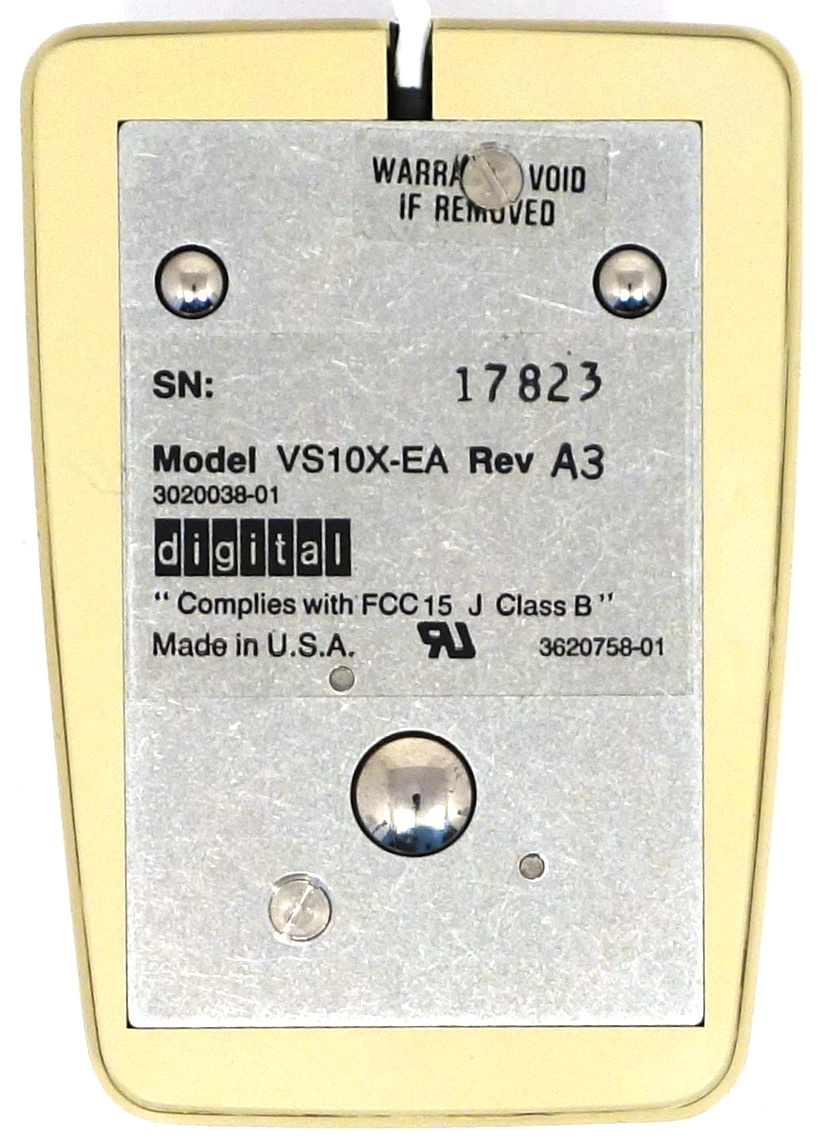
\includegraphics[scale=0.55]{1983_dec_vs10x_ea_mouse/bottom_30.jpg}
    \caption{DEC VS10X-EA Mouse, top and bottom views}
    \label{fig:DecVS10XTopAndBottom}
\end{figure}

The underside is made of metal (fig. \ref{fig:DecVS10XTopAndBottom}). The rotation is registered by a smooth steel ball in the center, while two smaller balls act as legs to minimize friction. The mouse was not supplied with a mouse pad, and  the VAXstation 100 user manual suggests to  put mouse on a plain sheet of paper \cite{manual}.

A removable ring that allows you to remove the ball to remove collected debris is not yet provided in this model, so complete disassembly is necessary for cleaning.

\begin{figure}[h]
    \centering
    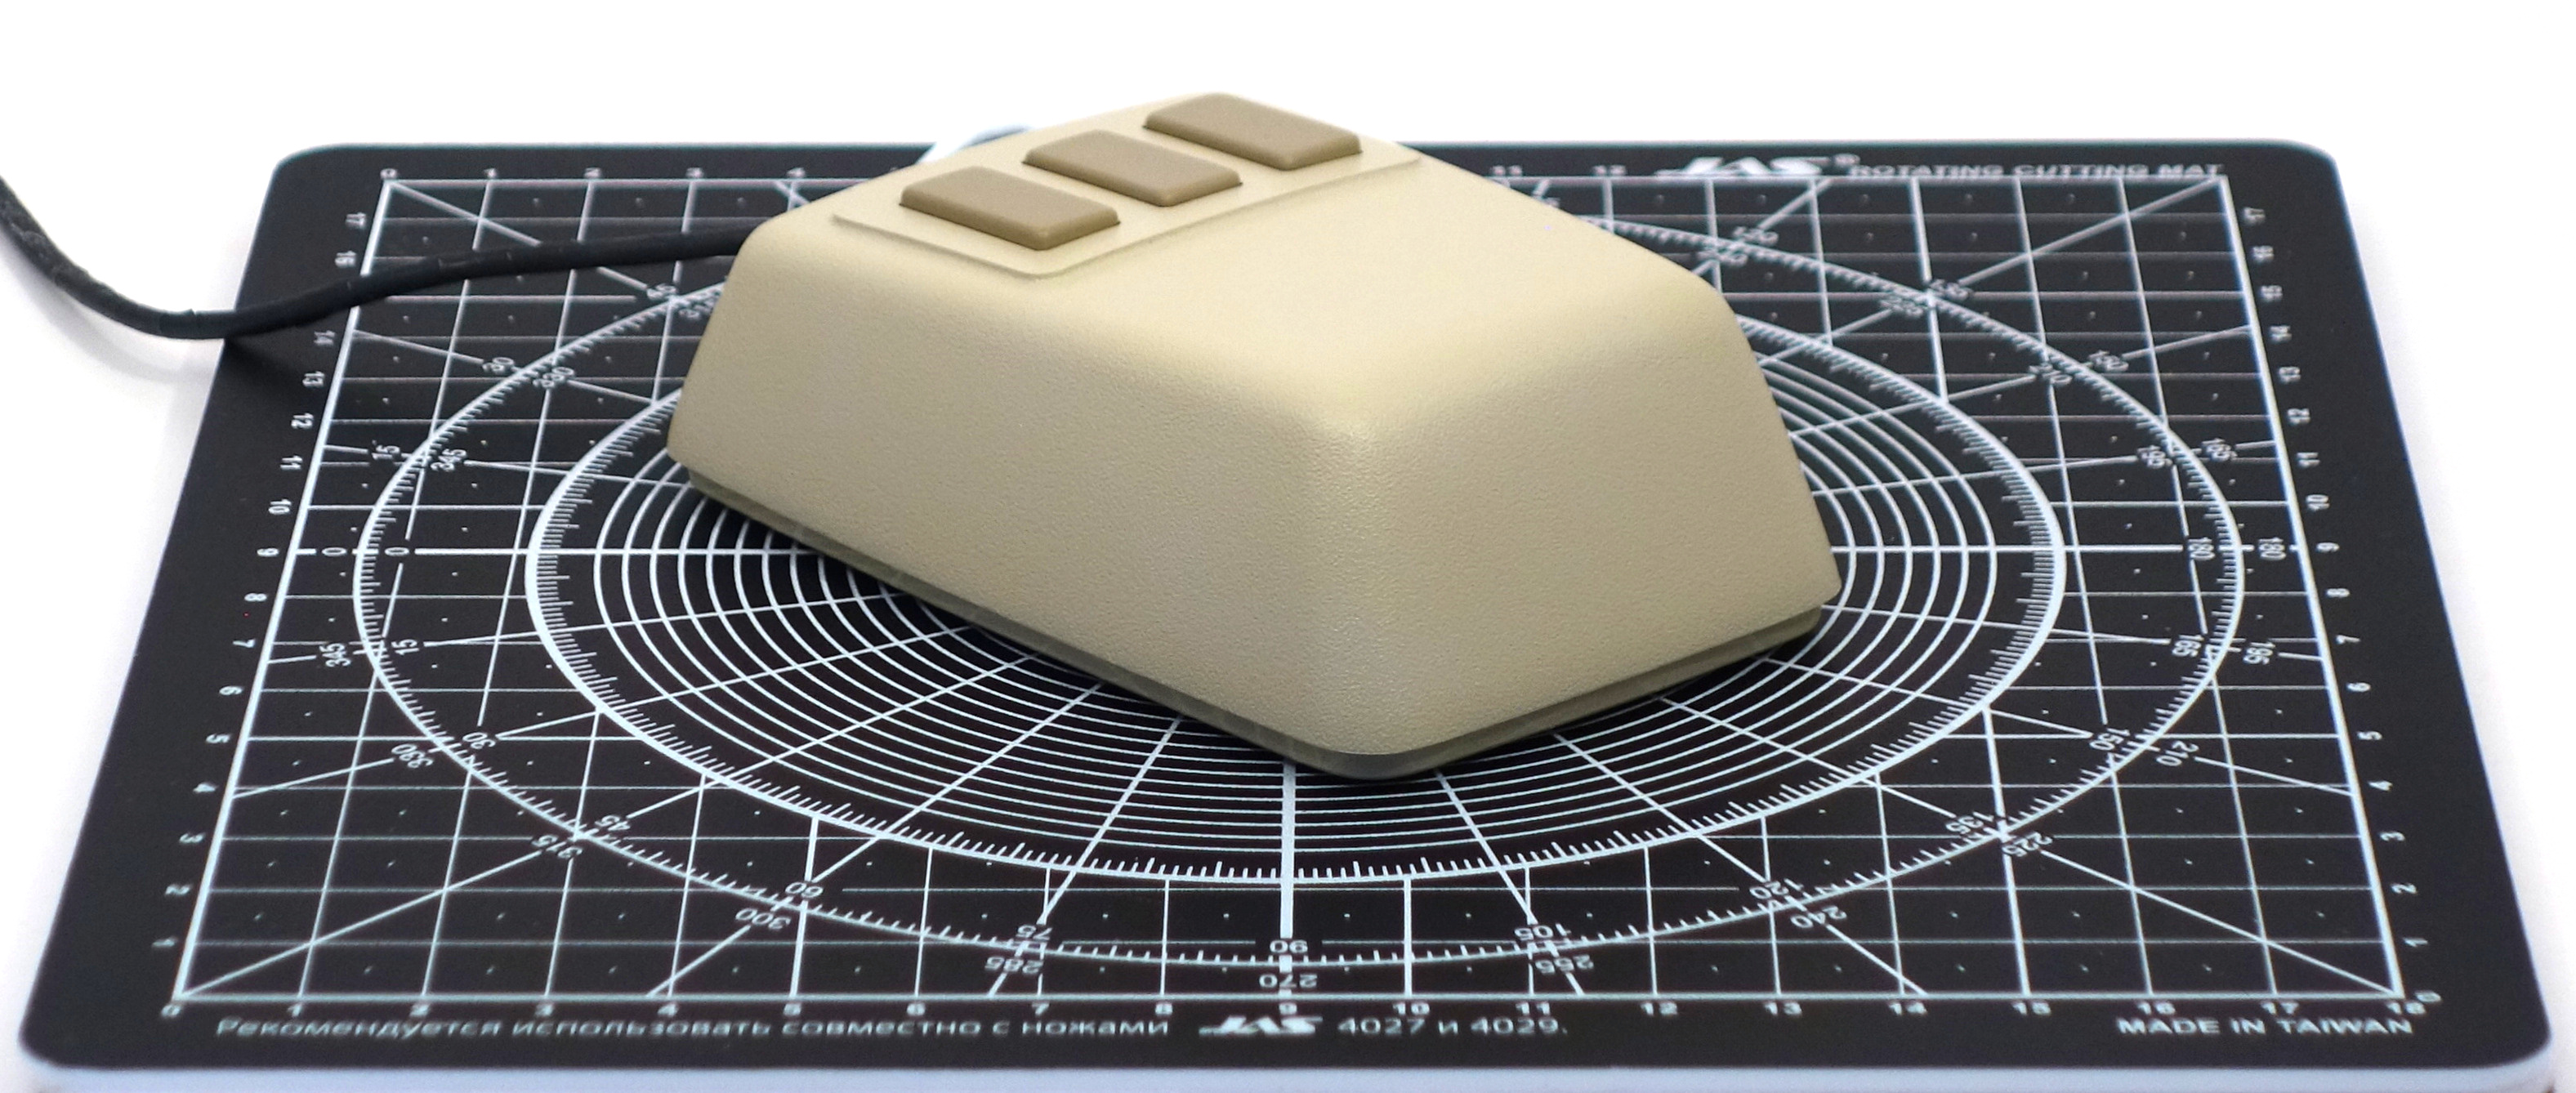
\includegraphics[scale=0.7]{1983_dec_vs10x_ea_mouse/size_30.jpg}
    \caption{DEC VS10X-EA on a graduated pad with a grid step of 1~cm}
    \label{fig:DecVS10XSize}
\end{figure}

The mouse has a small size, typical for mice of the 1980s (fig. \ref{fig:DecVS10XSize}), and so the hand can only lean on the body to a small extent (Fig. \ref{fig:DecVS10XHand}).
\begin{figure}[h]
    \centering
    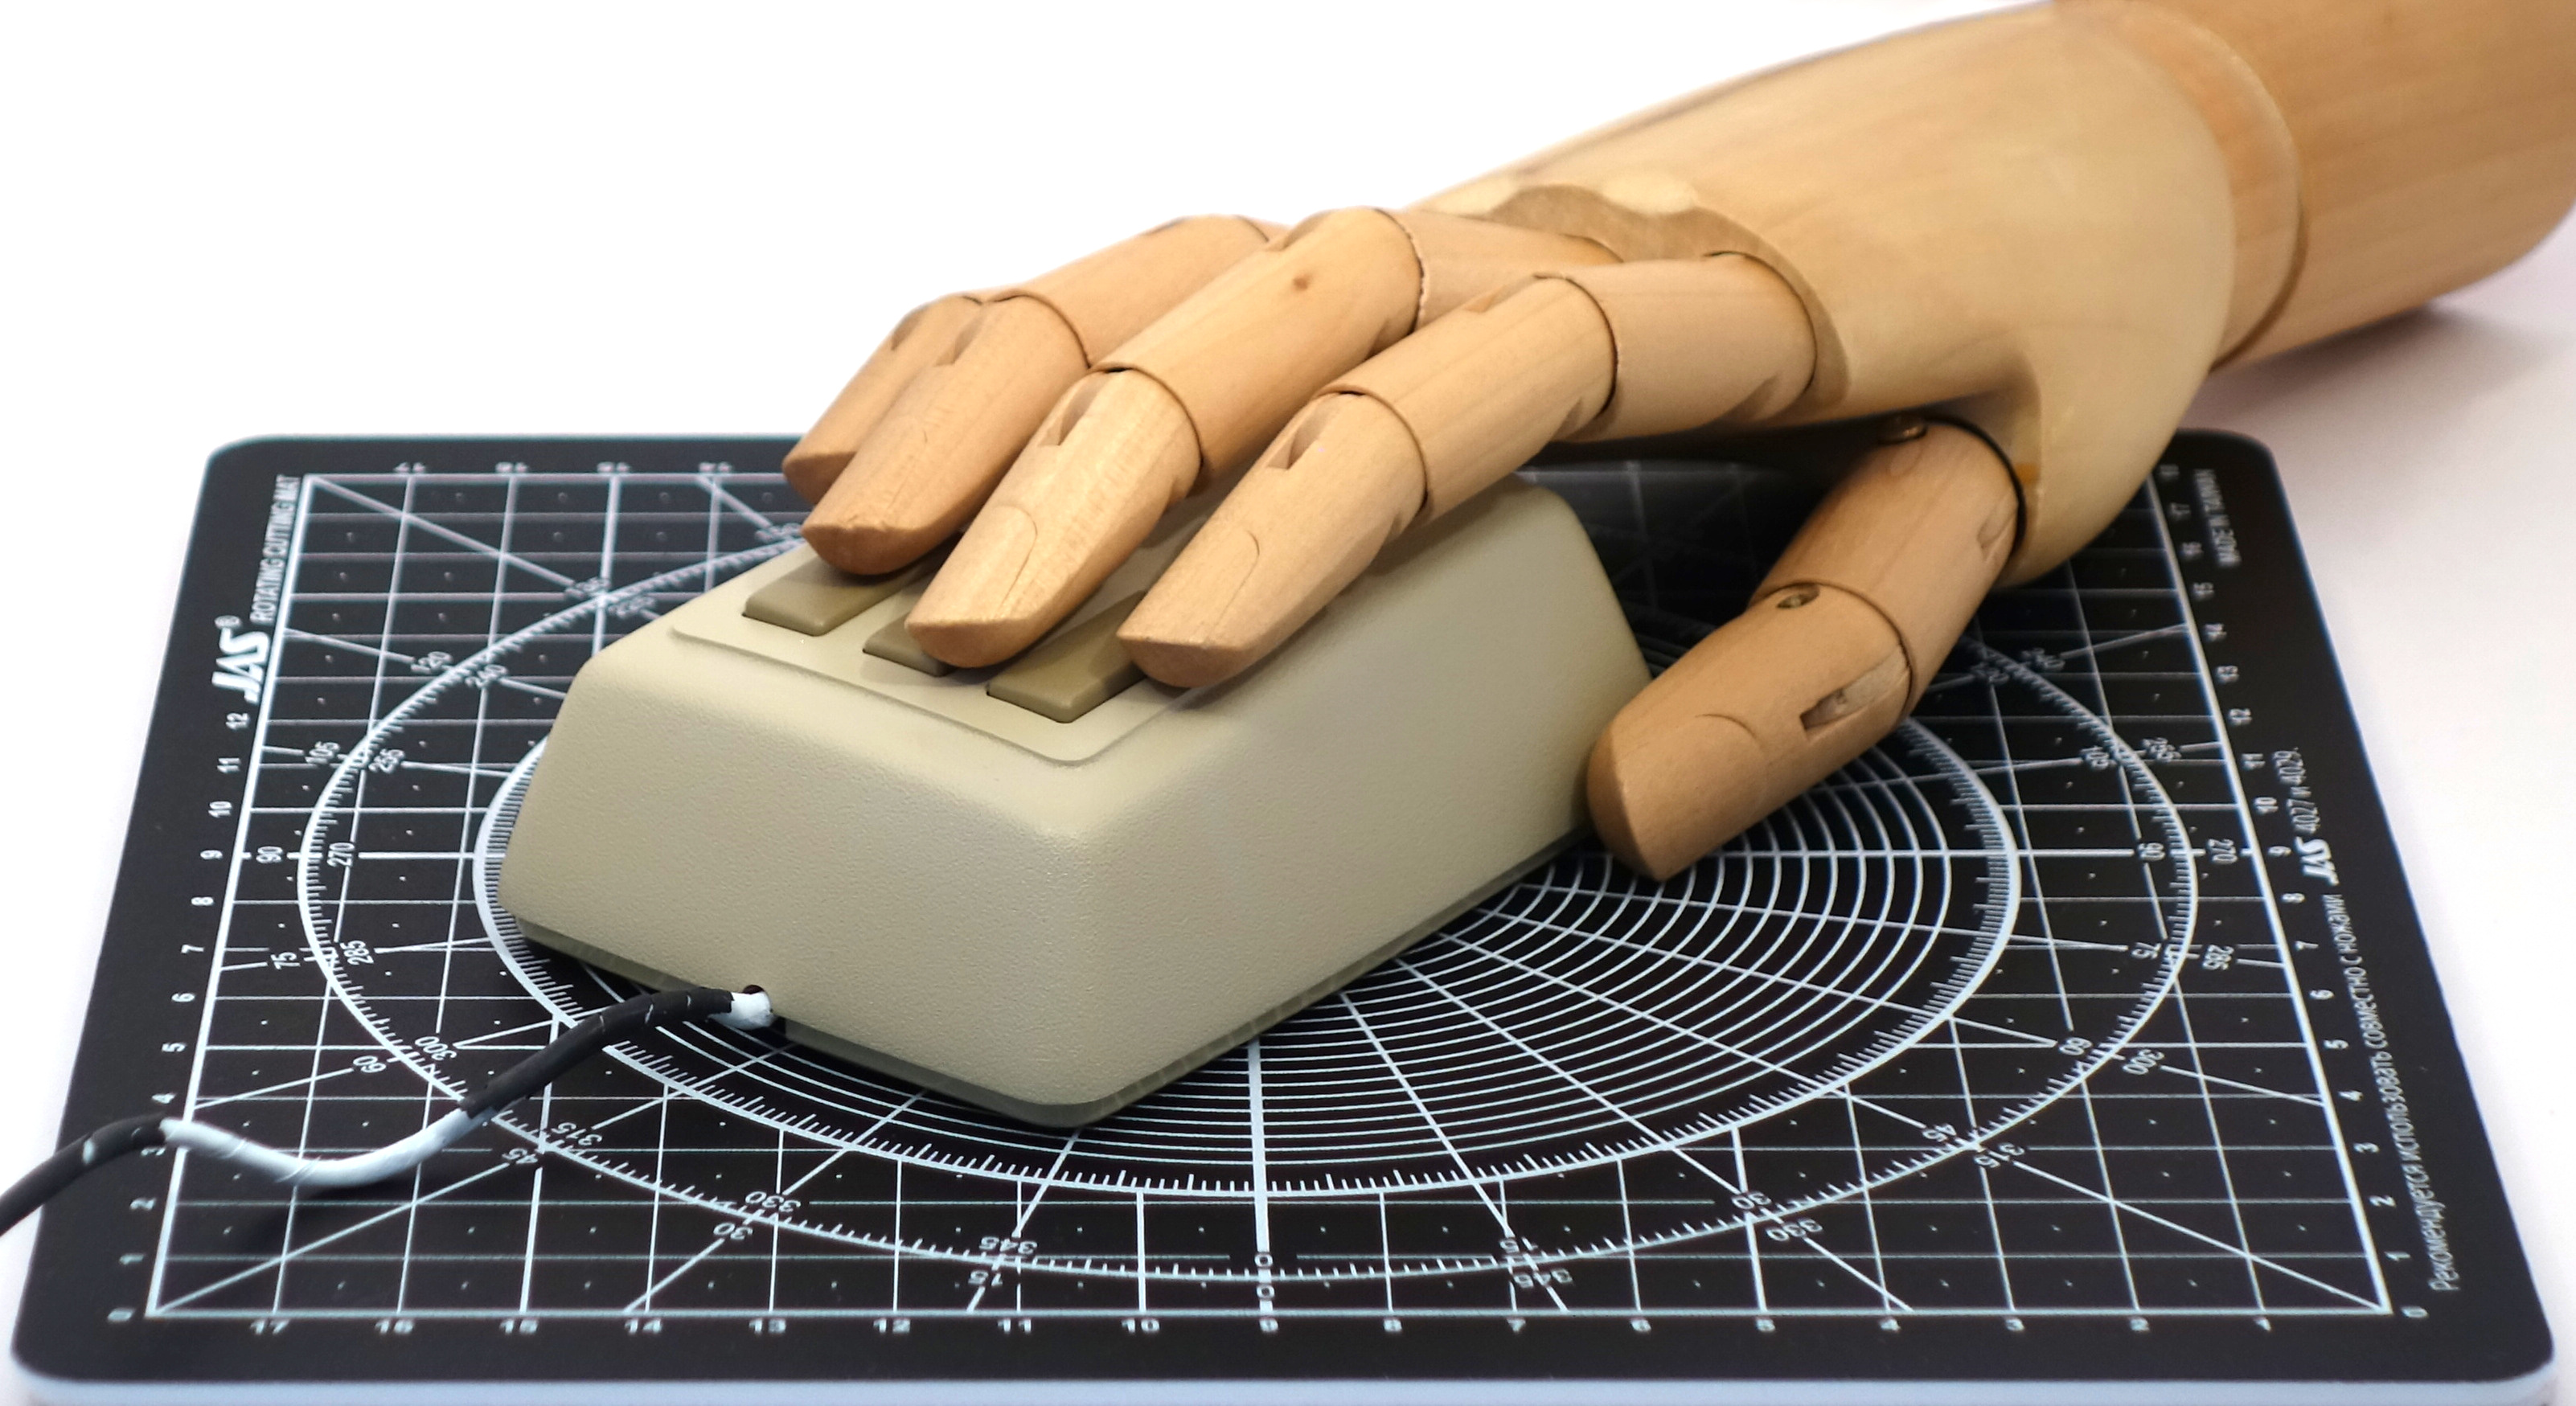
\includegraphics[scale=0.7]{1983_dec_vs10x_ea_mouse/hand_30.jpg}
    \caption{DEC VS10X-EAI with a human hand model}
    \label{fig:DecVS10XHand}
\end{figure}

Mouse internals are shown in figure \ref{fig:DecVS10XInside}. The removable solid protection of the ball is worthy of mention: it requires additional disassembly operations to remove garbage. In this mouse, contact encoders (with four contacts for greater reliability) are used, which are based on a metal contact drum instead of the more common disk in subsequent models.

~

\begin{figure}[h]
    \centering
    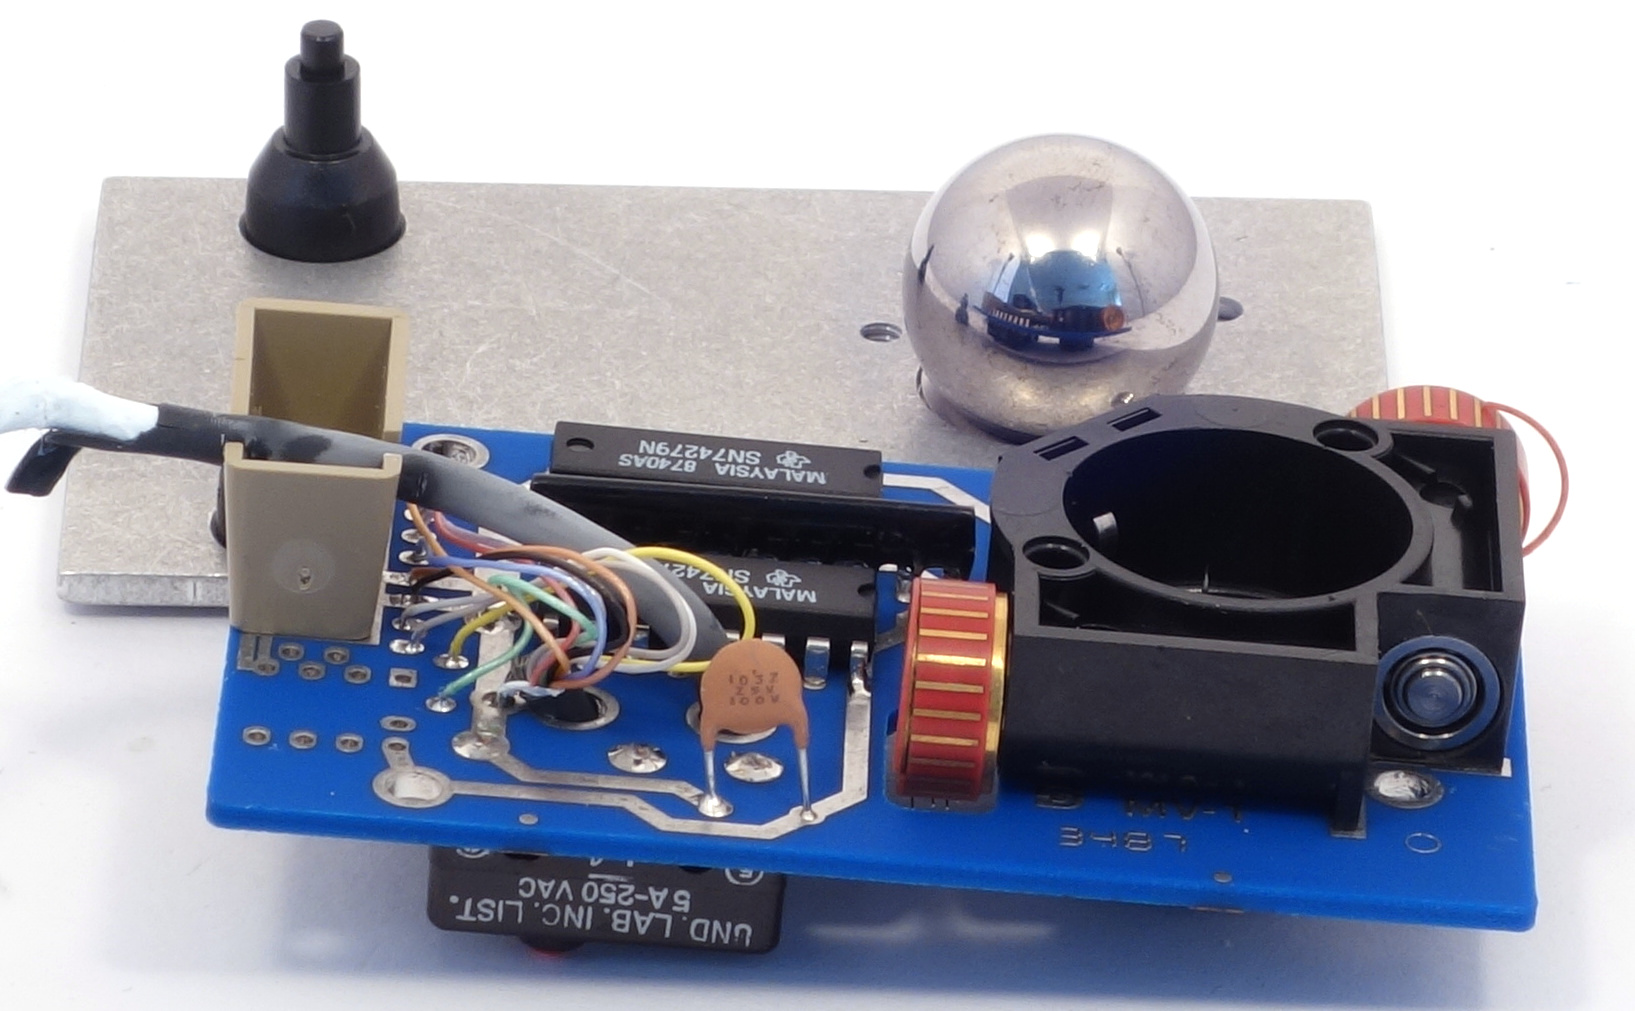
\includegraphics[scale=1]{1983_dec_vs10x_ea_mouse/inside_30.jpg}
    \caption{DEC VS10X-EA disassembled}
    \label{fig:DecVS10XInside}
\end{figure}

\begin{thebibliography}{9}
\bibitem{hawley} Hawley Mouse House \url{https://web.archive.org/web/20211020150835/https://oldmouse.com/mouse/hawley/}

\bibitem{mouses} Hawley Mark II X063X Mouses \url{https://web.archive.org/web/20211020000256/https://www.oldmouse.com/mouse/hawley/X063X.shtml}

\bibitem{pat} Transducer for a display-oriented pointing device \url{https://patents.google.com/patent/US3892963A/en}

\bibitem{reddit} Another DEC mouse \url{https://www.reddit.com/r/vintagecomputing/comments/mm4des/another_dec_mouse/}

\bibitem{manual} VAXstation 100 User Guide \url{http://www.bitsavers.org/pdf/dec/vax/vaxstation100/AA-N660A-TE_VAXstation_100_Users_Guide_Jun84.pdf}
\end{thebibliography}
\end{document}

\documentclass[11pt, a4paper]{article}
\usepackage{pdfpages}
\usepackage{parallel}
\usepackage[T2A]{fontenc}
\usepackage{ucs}
\usepackage[utf8x]{inputenc}
\usepackage[polish,english,russian]{babel}
\usepackage{hyperref}
\usepackage{rotating}
\usepackage[inner=2cm,top=1.8cm,outer=2cm,bottom=2.3cm,nohead]{geometry}
\usepackage{listings}
\usepackage{graphicx}
\usepackage{wrapfig}
\usepackage{longtable}
\usepackage{indentfirst}
\usepackage{array}
\usepackage{tikzsymbols}
\usepackage{soul}
\usepackage[ruled,vlined]{algorithm2e}
%\counterwithout{figure}{section} 

\usepackage{url}
\makeatletter
\g@addto@macro{\UrlBreaks}{\UrlOrds}
\makeatother

\newcolumntype{P}[1]{>{\raggedright\arraybackslash}p{#1}}
\frenchspacing
\usepackage{fixltx2e} %text sub- and superscripts
\usepackage{icomma} % коскі ў матэматычным рэжыме
\PreloadUnicodePage{4}

\newcommand{\longpage}{\enlargethispage{\baselineskip}}
\newcommand{\shortpage}{\enlargethispage{-\baselineskip}}

\def\switchlang#1{\expandafter\csname switchlang#1\endcsname}
\def\switchlangbe{
\let\saverefname=\refname%
\def\refname{Літаратура}%
\def\figurename{Іл.}%
}
\def\switchlangen{
\let\saverefname=\refname%
\def\refname{References}%
\def\figurename{Fig.}%
}
\def\switchlangru{
\let\saverefname=\refname%
\let\savefigurename=\figurename%
\def\refname{Литература}%
\def\figurename{Рис.}%
}

\hyphenation{admi-ni-stra-tive}
\hyphenation{ex-pe-ri-ence}
\hyphenation{fle-xi-bi-li-ty}
\hyphenation{Py-thon}
\hyphenation{ma-the-ma-ti-cal}
\hyphenation{re-ported}
\hyphenation{imp-le-menta-tions}
\hyphenation{pro-vides}
\hyphenation{en-gi-neering}
\hyphenation{com-pa-ti-bi-li-ty}
\hyphenation{im-pos-sible}
\hyphenation{desk-top}
\hyphenation{elec-tro-nic}
\hyphenation{com-pa-ny}
\hyphenation{de-ve-lop-ment}
\hyphenation{de-ve-loping}
\hyphenation{de-ve-lop}
\hyphenation{da-ta-ba-se}
\hyphenation{plat-forms}
\hyphenation{or-ga-ni-za-tion}
\hyphenation{pro-gramming}
\hyphenation{in-stru-ments}
\hyphenation{Li-nux}
\hyphenation{sour-ce}
\hyphenation{en-vi-ron-ment}
\hyphenation{Te-le-pathy}
\hyphenation{Li-nux-ov-ka}
\hyphenation{Open-BSD}
\hyphenation{Free-BSD}
\hyphenation{men-ti-on-ed}
\hyphenation{app-li-ca-tion}

\def\progref!#1!{\texttt{#1}}
\renewcommand{\arraystretch}{2} %Іначай формулы ў матрыцы зліпаюцца з лініямі
\usepackage{array}

\def\interview #1 (#2), #3, #4, #5\par{

\section[#1, #3, #4]{#1 -- #3, #4}
\def\qname{LVEE}
\def\aname{#1}
\def\q ##1\par{{\noindent \bf \qname: ##1 }\par}
\def\a{{\noindent \bf \aname: } \def\qname{L}\def\aname{#2}}
}

\def\interview* #1 (#2), #3, #4, #5\par{

\section*{#1\\{\small\rm #3, #4. #5}}
\ifx\ParallelWhichBox\undefined%
    \addcontentsline{toc}{section}{#1, #3, #4}%
\else%
\ifnum\ParallelWhichBox=0%
    \addcontentsline{toc}{section}{#1, #3, #4}%
\fi\fi%

\def\qname{LVEE}
\def\aname{#1}
\def\q ##1\par{{\noindent \bf \qname: ##1 }\par}
\def\a{{\noindent \bf \aname: } \def\qname{L}\def\aname{#2}}
}

\newcommand{\interviewfooter}[1]{
\vskip 1em
\noindent \textit{#1}
}


\begin{document}

\title{1983 "--- Logitech LOGIMOUSE P5}
\date{}
\maketitle

LOGIMOUSE P5 mouse was released in 1983. This is the second manipulator from Logitech (after the famous  P4 mouse, production of which continued simultaneously with P5). LOGIMOUSE P5 was a cheaper model (the selling price differed by \$100), and it was intended primarily for OEM supplies. But the main feature of the P5 is a radically different exterior (fig. \ref{fig:LogimouseP5Pic}).

\begin{figure}[h]
   \centering
    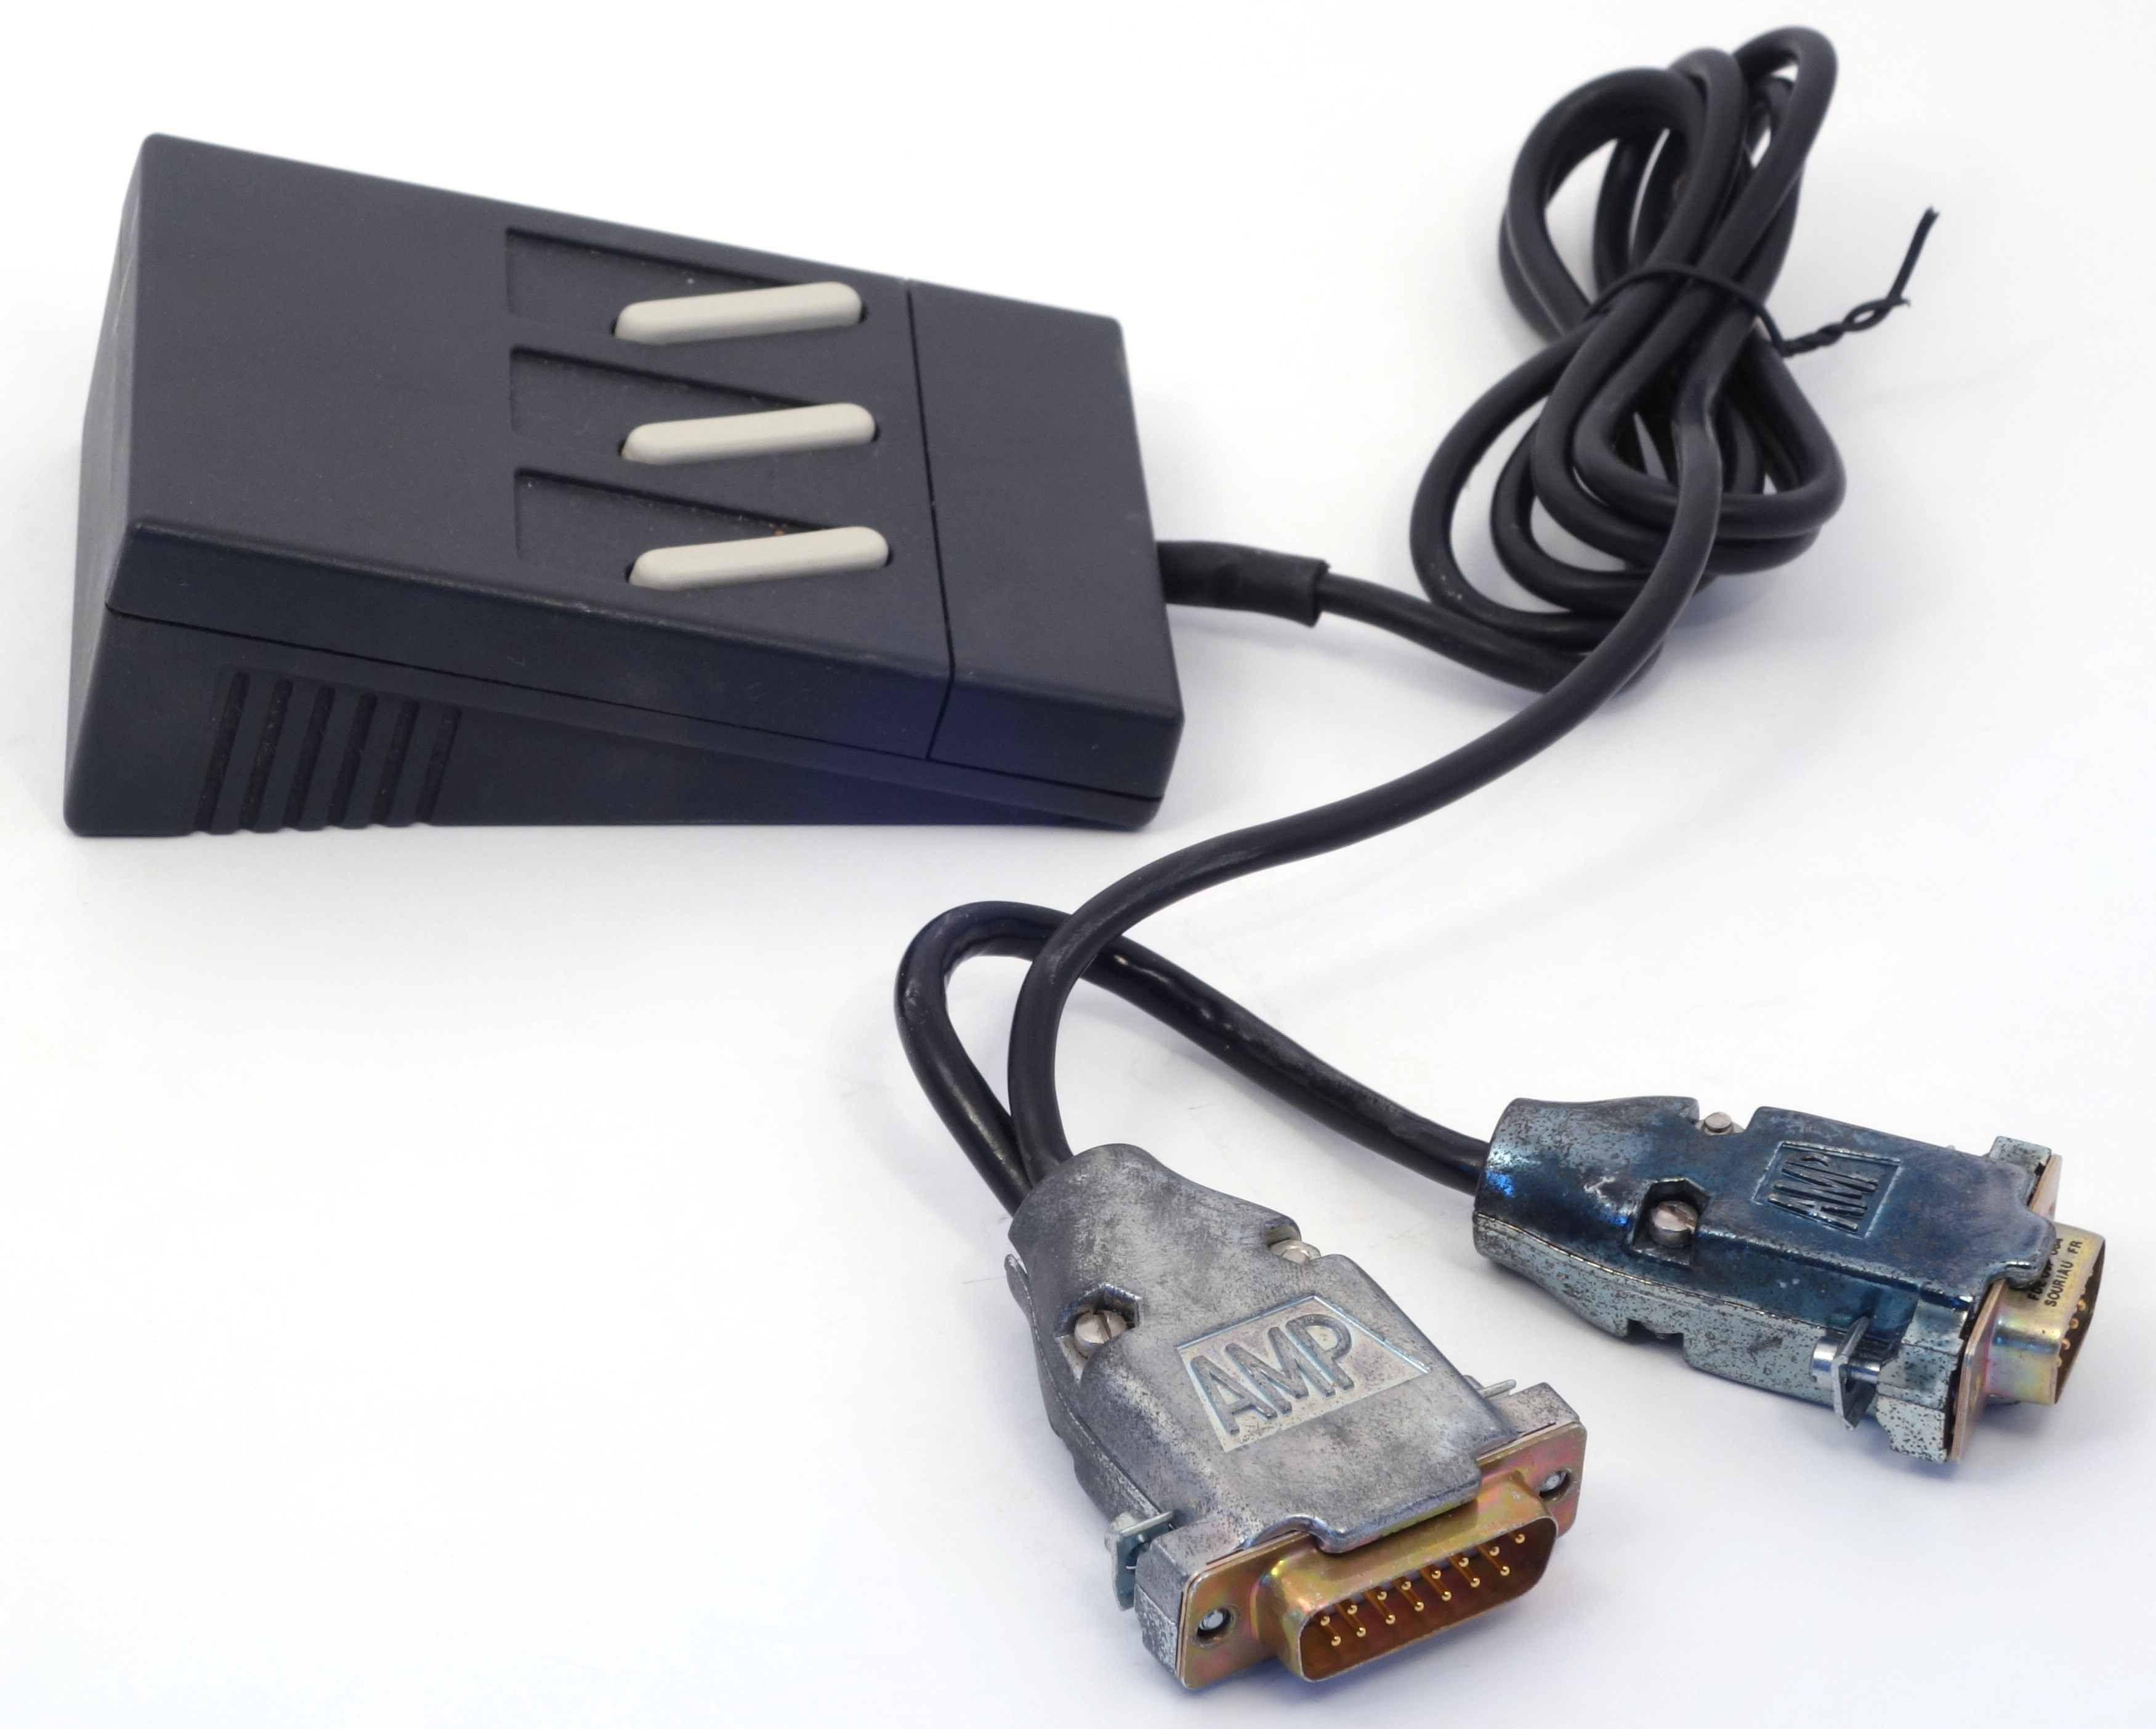
\includegraphics[scale=0.35]{1983_logitech_logimouse_p5/pic_30.jpg}
    \caption{LOGIMOUSE P5}
    \label{fig:LogimouseP5Pic}
\end{figure}

The mouse has a defiant design look, although in 1983 this concept did not yet exist in relation to mice: three narrow white buttons are placed diagonally on a black prismatic body with a reverse slope. On the underside, there are four low-friction white supports (which are also PCB mounts) and a brushed metal ball (fig. \ref{fig:LogimouseP5TopAndBottom}). A removable turnable ring with latches allows you to remove the ball to get rid of accumulated dirt and to clean the rollers. Logitech P4 and other mice of the first half of the 80s did not have a ring or it had to be unscrewed with a screwdriver. Therefore, P5 is one of the first cases (along with the Apple Lisa mouse released in the same year) to use this turnable ring, which later became the standard.

\begin{figure}[h]
    \centering
    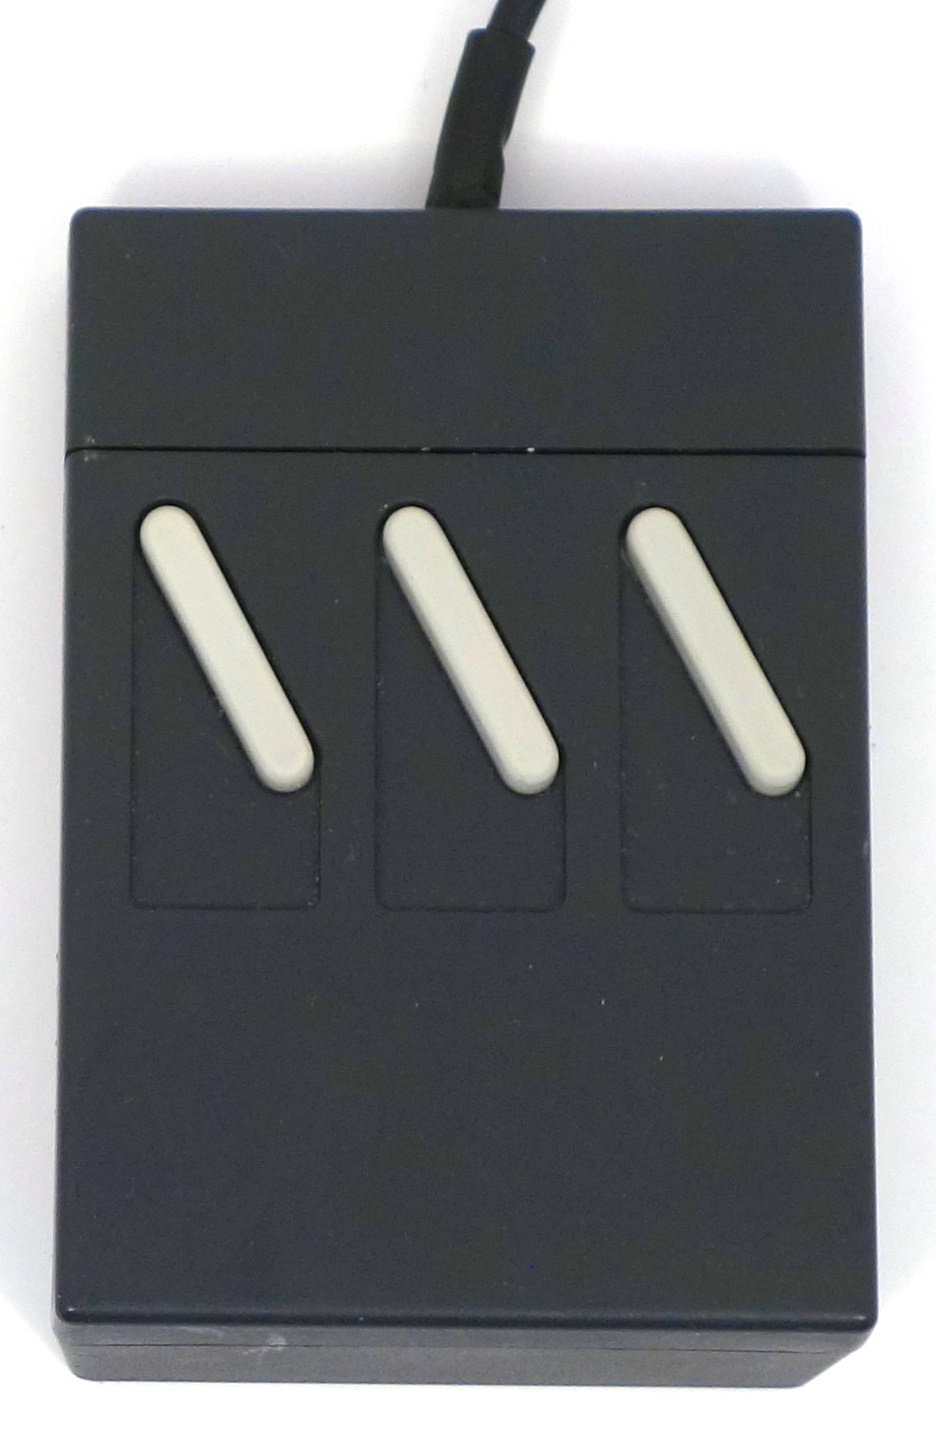
\includegraphics[scale=0.4]{1983_logitech_logimouse_p5/top_30.jpg}
    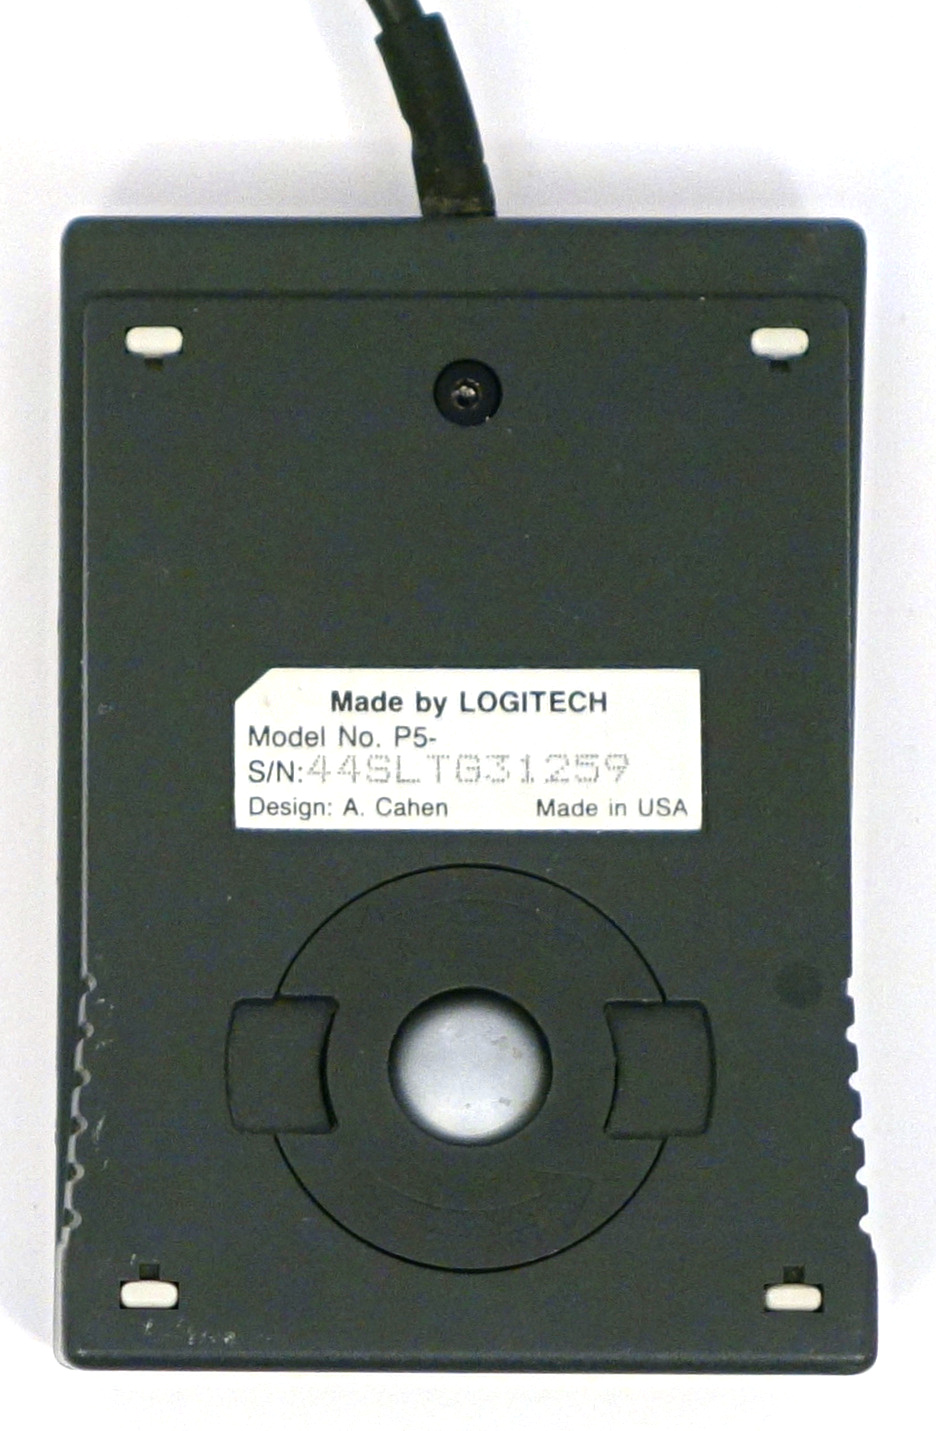
\includegraphics[scale=0.4]{1983_logitech_logimouse_p5/bottom_30.jpg}
    \caption{LOGIMOUSE P5, top and bottom views}
    \label{fig:LogimouseP5TopAndBottom}
\end{figure}

Judging by the cable with two connectors, this is a mouse from FutureNet "---a workstation for microelectronics CAD. This computer was a classic IBM PC with a monochrome text video adapter and an additional graphics card with a resolution of 640x360 pixels, and the fifteen-pin connector on the mouse cable was used to to connect the output of an IBM monochrome video adapter to a graphics card. This allowed the display to be used alternately for text output and for graphics output by the schematic editor \cite{futurenet}.

\begin{figure}[h]
    \centering
    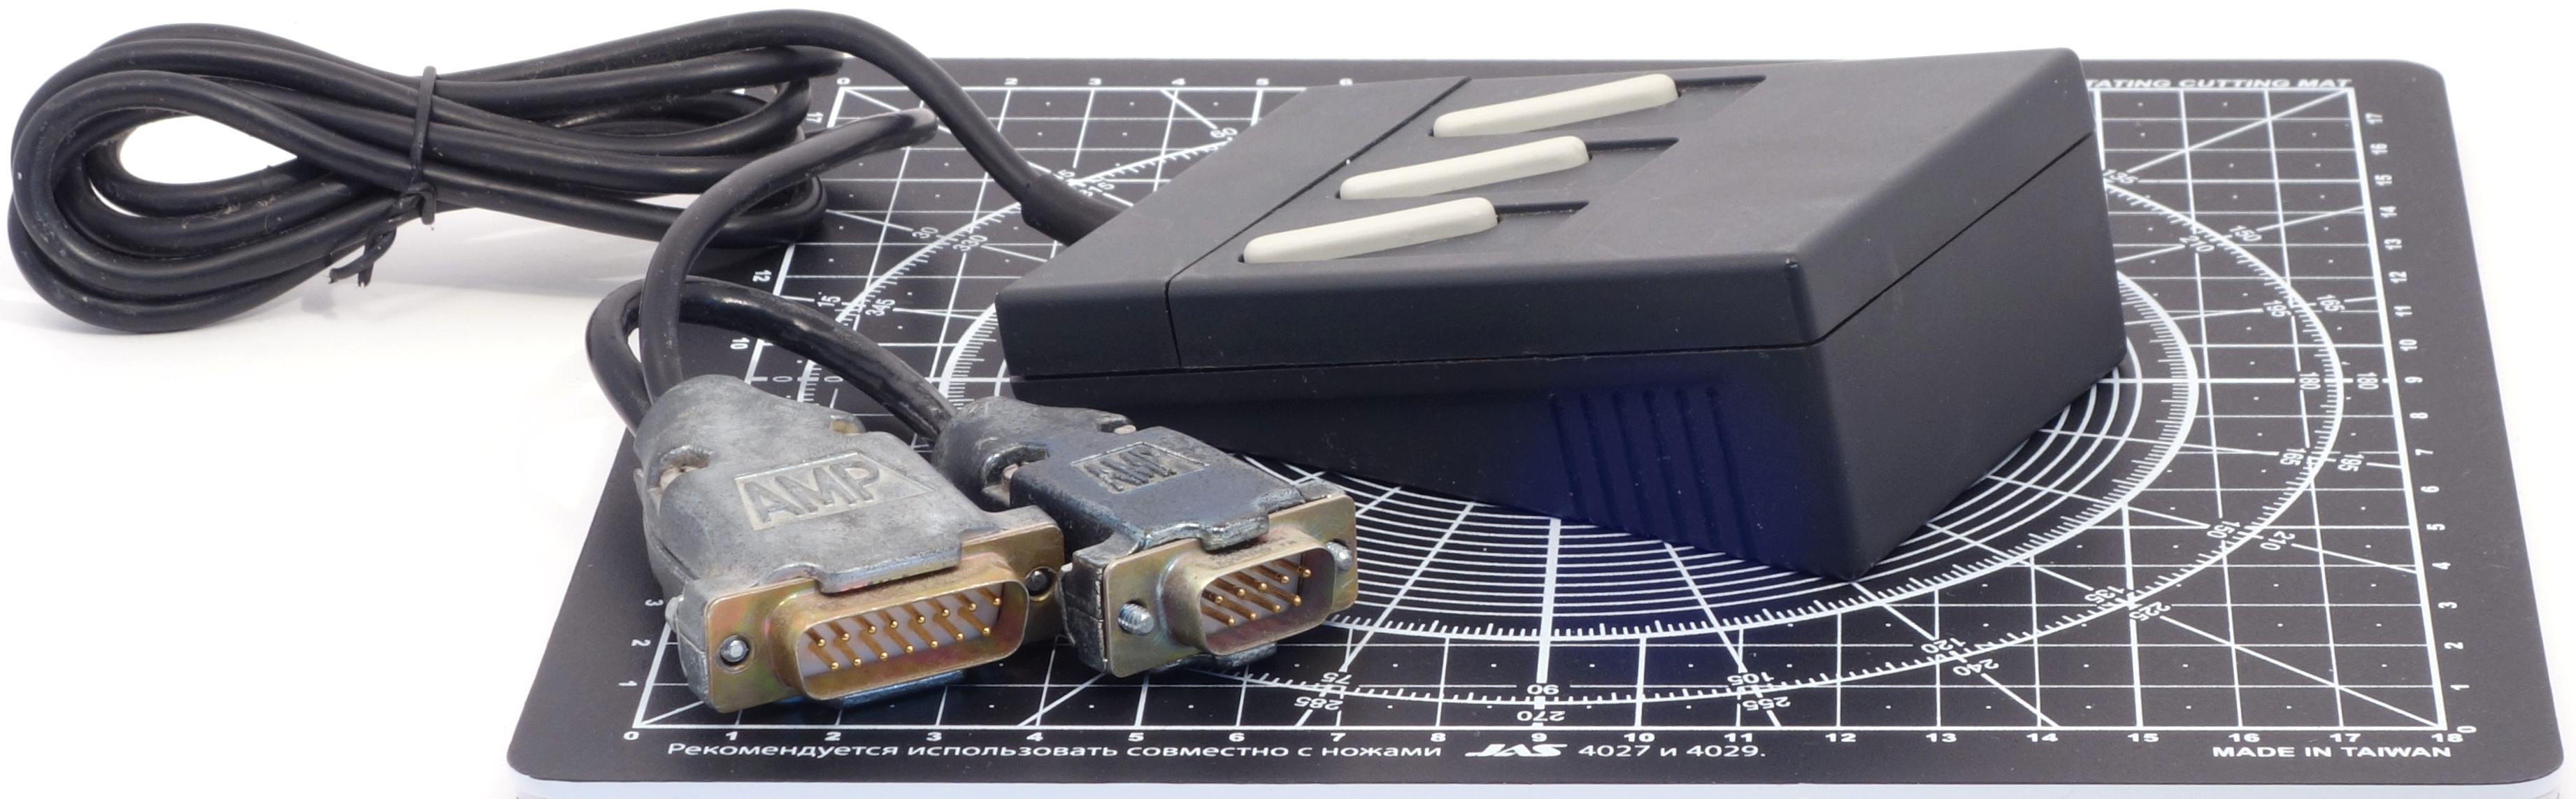
\includegraphics[scale=0.5]{1983_logitech_logimouse_p5/size_30.jpg}
    \caption{LOGIMOUSE P5 on a graduated pad with a grid step of 1~cm}
    \label{fig:LogimouseP5Size}
\end{figure}

The size of the mouse is typical for mice from the 1980s (fig. \ref{fig:LogimouseP5Size}). In fact, its dimensions are close to the later Logitech P7 and its most mass-produced variant, the C7. As for ergonomics, it is obvious that the prismatic case and diagonal narrow buttons had a very negative effect: when placing fingers along the buttons, the palm runs the risk of leaning on the protruding corner of the case; placing the palm along the lines of the body improves the situation only slightly, instead making it more difficult to press the already inconvenient buttons (Fig. \ref{fig:LogimouseP5Hand}).

\begin{figure}[h]
    \centering
    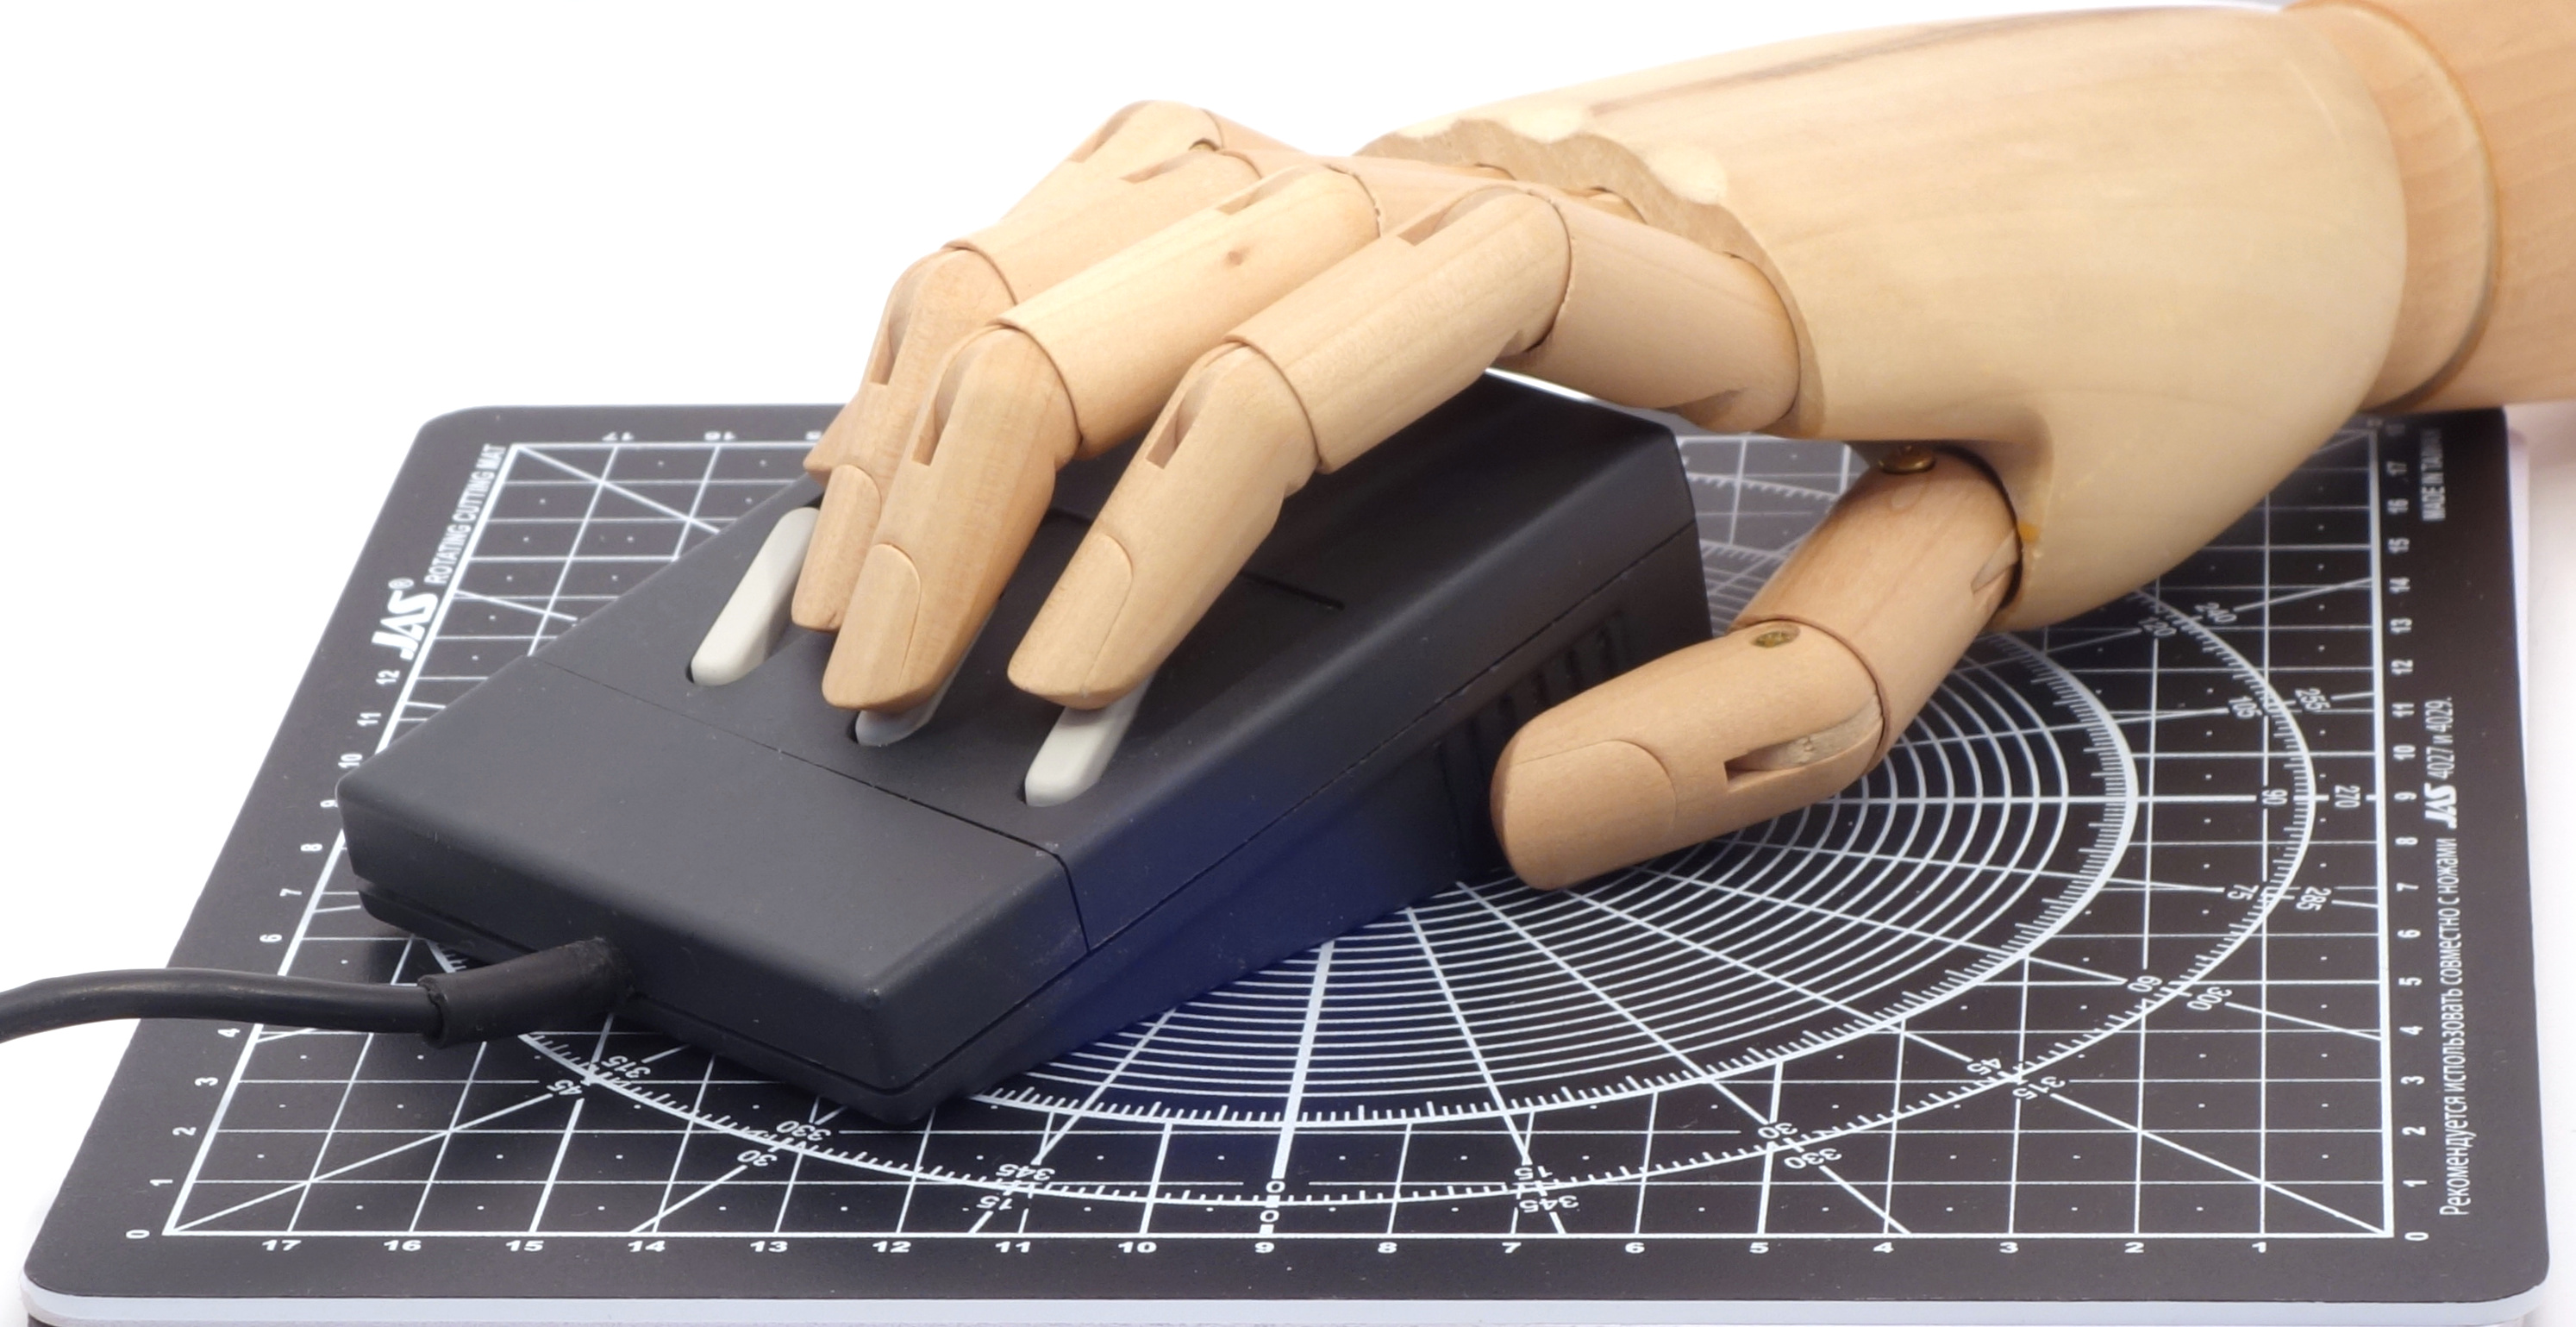
\includegraphics[scale=0.5]{1983_logitech_logimouse_p5/hand_30.jpg}
    \caption{LOGIMOUSE P5 with a human hand model}
    \label{fig:LogimouseP5Hand}
\end{figure}

Electrically, the P5 is similar to the Logitech P4 mouse, but has a lower resolution (200 DPI vs. 381 DPI). As an additional accessory, both mice were sometimes equipped with a special LogiMate \cite{oldmouse} converter, which allowed the mouse to be connected not to a separate adapter with a bus interface, but to a keyboard cable. With this connected, moving the mouse resulted in generating cursor key codes:  the resolution was 12 keypresses per inch horizontally and 6 keypresses vertically by default, which was designed to work in 80x25 character text mode. PC Magazine's review noted that using a mouse in standard mode made it possible to move the cursor in a text editor seven times faster than using the corresponding keys on the keyboard (however, it took getting used to the fact that as a result of a slight movement of the mouse over the rightmost position, the text editor cursor immediately jumped to the left position of the next line). For obvious reasons, this use of the mouse did not require a driver; however, its use gave the possibility of additional settings "--- for example, it allowed to set the resolution of the LogiMate adapter in the range of 1--100 keypresses per inch, as well as reassign the action of the mouse keys (key codes F8, F9 and F10 were generated by default) \cite{logimouse}.

 \begin{figure}[h]
    \centering
    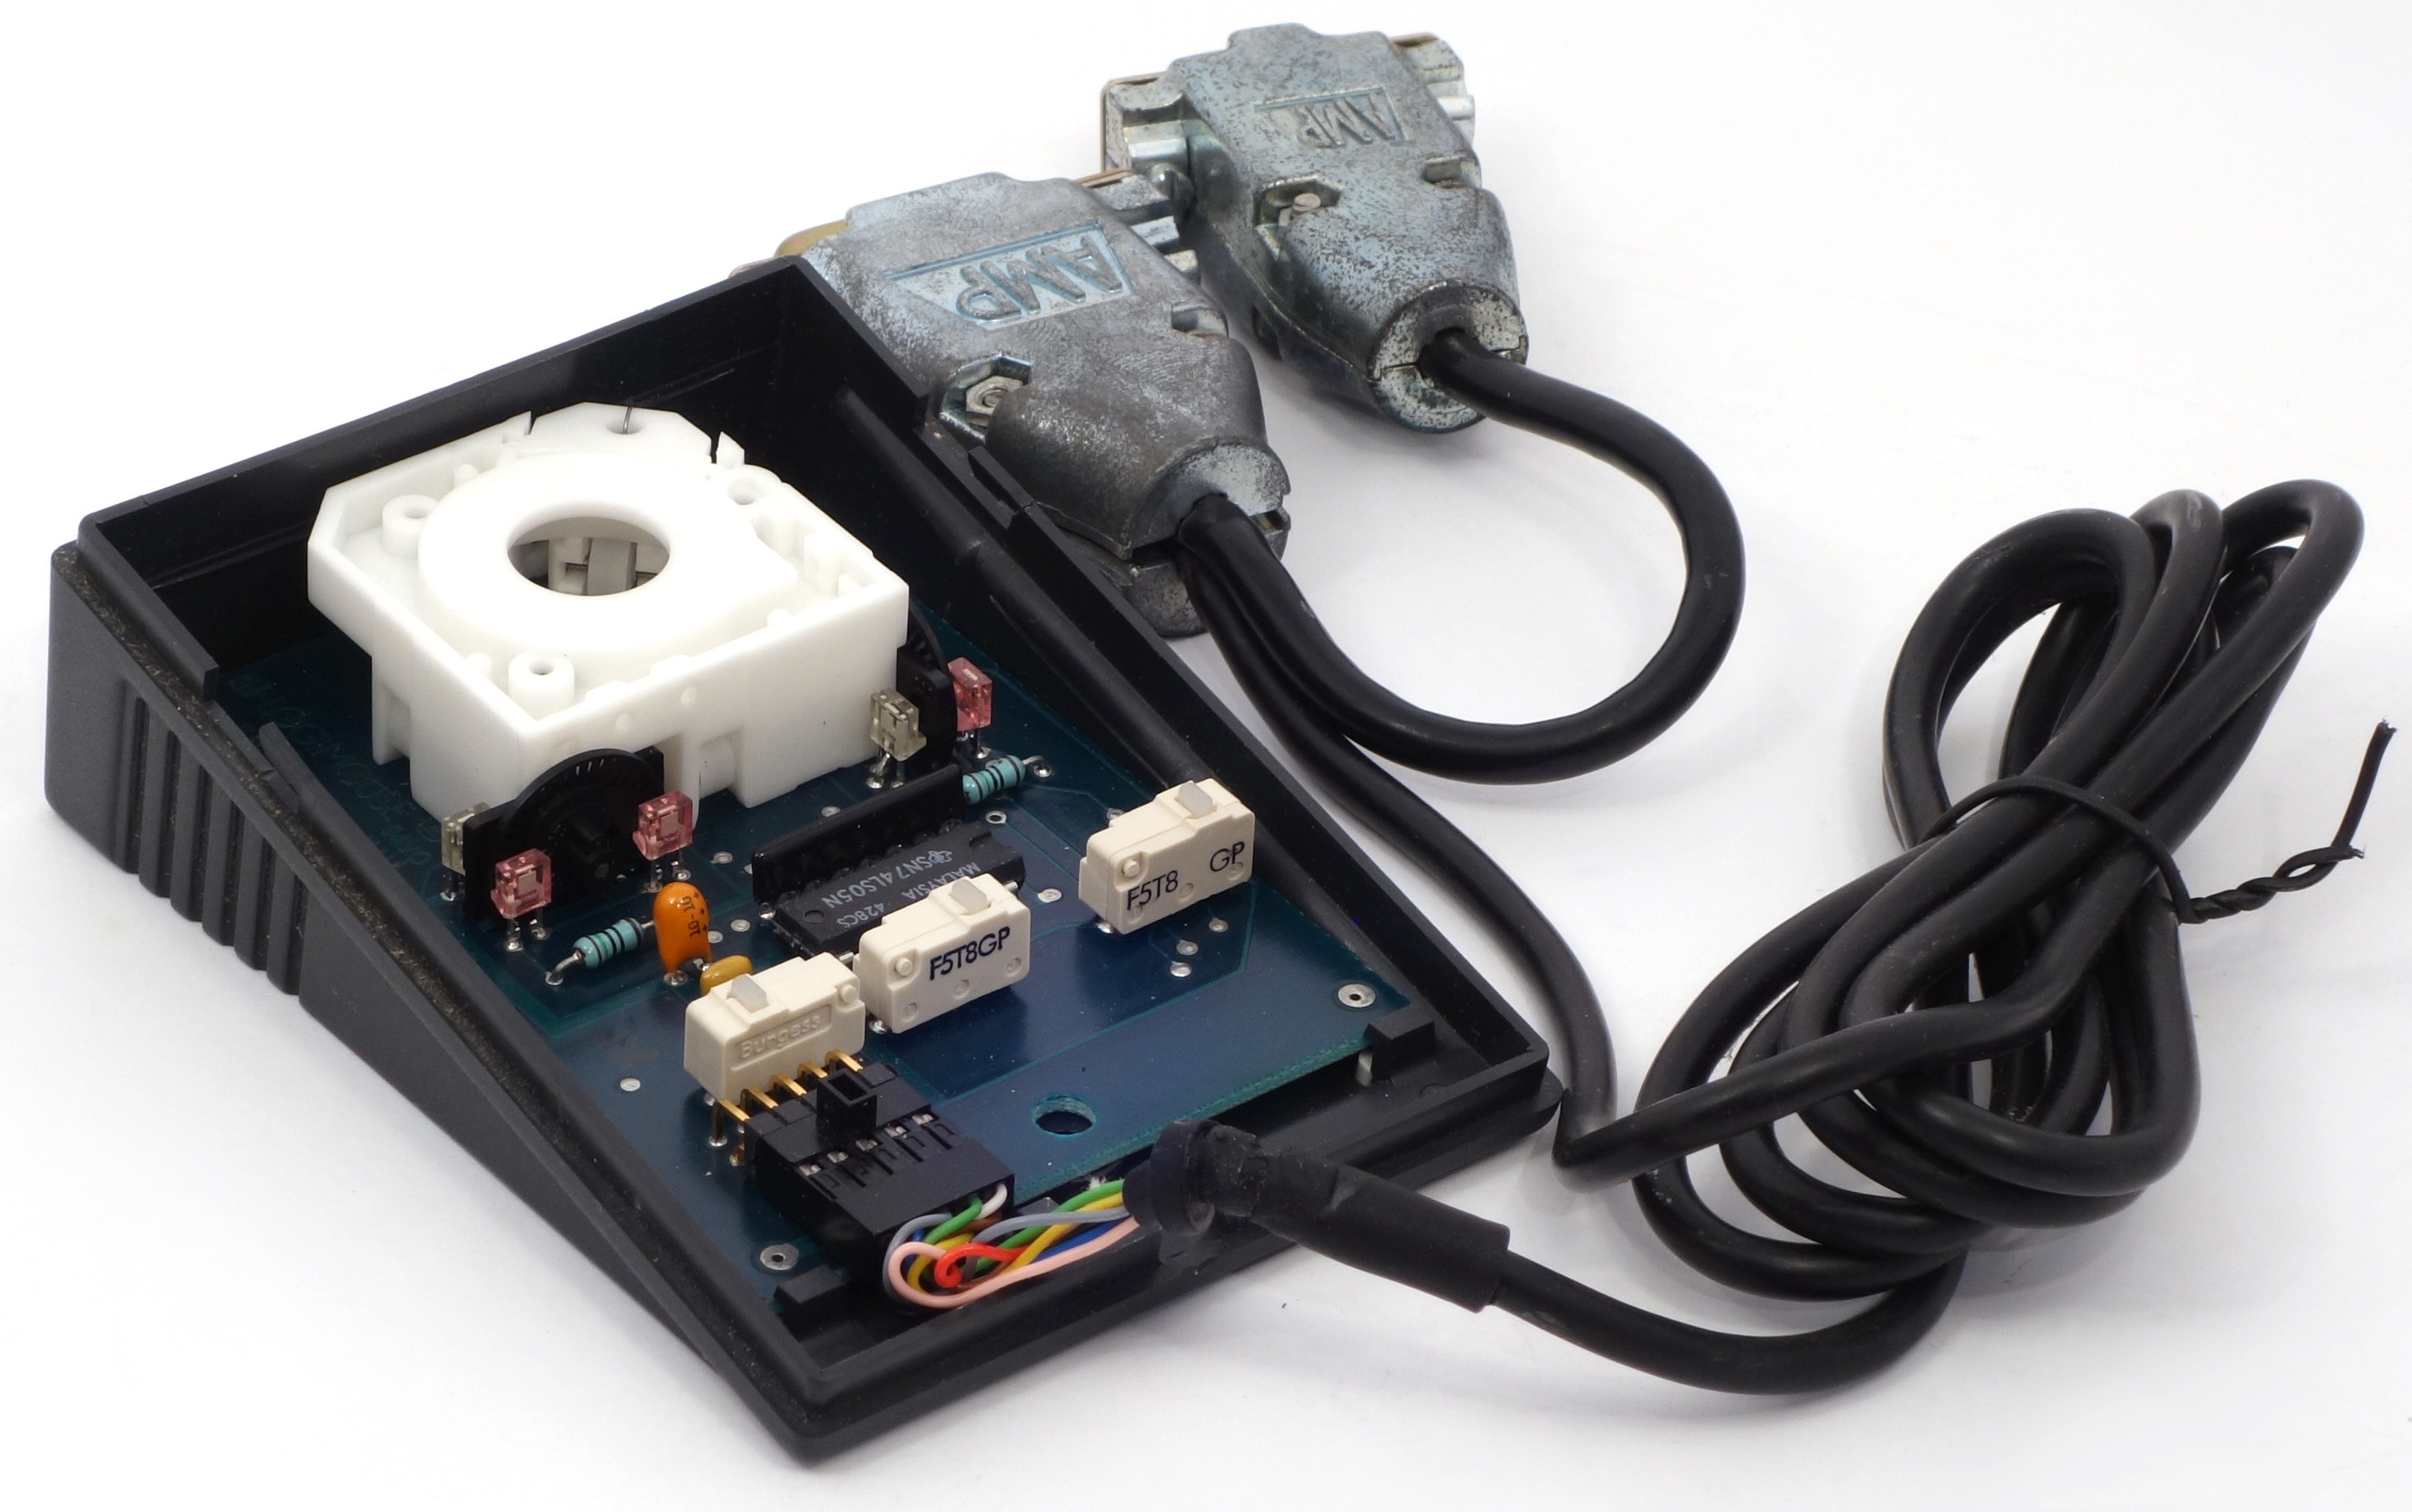
\includegraphics[scale=0.7]{1983_logitech_logimouse_p5/inside_30.jpg}
    \caption{LOGIMOUSE P5 disassembled}
    \label{fig:LogimouseP5Inside}
\end{figure}

The internal structure of the mouse is shown in fig. \ref{fig:LogimouseP5Inside}. The mouse uses optomechanical encoders.The optocouples and the optical interrupter disk are very similar to the corresponding parts in the mice of the 90-s (this can be considered one of the first such implementations). A distinctive feature of the encoder (as in P4 model) is an additional fixed mask that reduces the area of flare.

\begin{thebibliography}{9}
\bibitem {logimouse} J. Taylor. Faster then a speeding cursor key. // PC Magazine, V. 3, No. 2, February 7, 1984. - p. 243-245 \url{https://archive.org/details/PC-Mag-1984-02-07/page/n243/mode/2up}
\bibitem {futurenet} M. Holley. Logitech Logimouse Cable 1983 \url{https://commons.wikimedia.org/wiki/File:Logitech_Logimouse_Cable_1983.jpg}
\end{thebibliography}
\end{document}

\documentclass[11pt, a4paper]{article}
\usepackage{pdfpages}
\usepackage{parallel}
\usepackage[T2A]{fontenc}
\usepackage{ucs}
\usepackage[utf8x]{inputenc}
\usepackage[polish,english,russian]{babel}
\usepackage{hyperref}
\usepackage{rotating}
\usepackage[inner=2cm,top=1.8cm,outer=2cm,bottom=2.3cm,nohead]{geometry}
\usepackage{listings}
\usepackage{graphicx}
\usepackage{wrapfig}
\usepackage{longtable}
\usepackage{indentfirst}
\usepackage{array}
\usepackage{tikzsymbols}
\usepackage{soul}
\usepackage[ruled,vlined]{algorithm2e}
%\counterwithout{figure}{section} 

\usepackage{url}
\makeatletter
\g@addto@macro{\UrlBreaks}{\UrlOrds}
\makeatother

\newcolumntype{P}[1]{>{\raggedright\arraybackslash}p{#1}}
\frenchspacing
\usepackage{fixltx2e} %text sub- and superscripts
\usepackage{icomma} % коскі ў матэматычным рэжыме
\PreloadUnicodePage{4}

\newcommand{\longpage}{\enlargethispage{\baselineskip}}
\newcommand{\shortpage}{\enlargethispage{-\baselineskip}}

\def\switchlang#1{\expandafter\csname switchlang#1\endcsname}
\def\switchlangbe{
\let\saverefname=\refname%
\def\refname{Літаратура}%
\def\figurename{Іл.}%
}
\def\switchlangen{
\let\saverefname=\refname%
\def\refname{References}%
\def\figurename{Fig.}%
}
\def\switchlangru{
\let\saverefname=\refname%
\let\savefigurename=\figurename%
\def\refname{Литература}%
\def\figurename{Рис.}%
}

\hyphenation{admi-ni-stra-tive}
\hyphenation{ex-pe-ri-ence}
\hyphenation{fle-xi-bi-li-ty}
\hyphenation{Py-thon}
\hyphenation{ma-the-ma-ti-cal}
\hyphenation{re-ported}
\hyphenation{imp-le-menta-tions}
\hyphenation{pro-vides}
\hyphenation{en-gi-neering}
\hyphenation{com-pa-ti-bi-li-ty}
\hyphenation{im-pos-sible}
\hyphenation{desk-top}
\hyphenation{elec-tro-nic}
\hyphenation{com-pa-ny}
\hyphenation{de-ve-lop-ment}
\hyphenation{de-ve-loping}
\hyphenation{de-ve-lop}
\hyphenation{da-ta-ba-se}
\hyphenation{plat-forms}
\hyphenation{or-ga-ni-za-tion}
\hyphenation{pro-gramming}
\hyphenation{in-stru-ments}
\hyphenation{Li-nux}
\hyphenation{sour-ce}
\hyphenation{en-vi-ron-ment}
\hyphenation{Te-le-pathy}
\hyphenation{Li-nux-ov-ka}
\hyphenation{Open-BSD}
\hyphenation{Free-BSD}
\hyphenation{men-ti-on-ed}
\hyphenation{app-li-ca-tion}

\def\progref!#1!{\texttt{#1}}
\renewcommand{\arraystretch}{2} %Іначай формулы ў матрыцы зліпаюцца з лініямі
\usepackage{array}

\def\interview #1 (#2), #3, #4, #5\par{

\section[#1, #3, #4]{#1 -- #3, #4}
\def\qname{LVEE}
\def\aname{#1}
\def\q ##1\par{{\noindent \bf \qname: ##1 }\par}
\def\a{{\noindent \bf \aname: } \def\qname{L}\def\aname{#2}}
}

\def\interview* #1 (#2), #3, #4, #5\par{

\section*{#1\\{\small\rm #3, #4. #5}}
\ifx\ParallelWhichBox\undefined%
    \addcontentsline{toc}{section}{#1, #3, #4}%
\else%
\ifnum\ParallelWhichBox=0%
    \addcontentsline{toc}{section}{#1, #3, #4}%
\fi\fi%

\def\qname{LVEE}
\def\aname{#1}
\def\q ##1\par{{\noindent \bf \qname: ##1 }\par}
\def\a{{\noindent \bf \aname: } \def\qname{L}\def\aname{#2}}
}

\newcommand{\interviewfooter}[1]{
\vskip 1em
\noindent \textit{#1}
}

\switchlang{en}
\begin{document}

\title{1986 "--- Commodore C300 mouse}
\date{}
\maketitle
\selectlanguage{english}
The Commodore C300 mouse labeled Joystick Mouse on the box is one of the reincarnations of the Kempston Mouse released in 1986 for ZX Spectrum computers \cite{SinclairUser}, adapted for Commodore computers \cite{c64wiki}. Externally, the mouse looks typical, having two buttons on top and a ball on the bottom (figure \ref{fig:C300Pic}).

\begin{figure}[h]
    \centering
    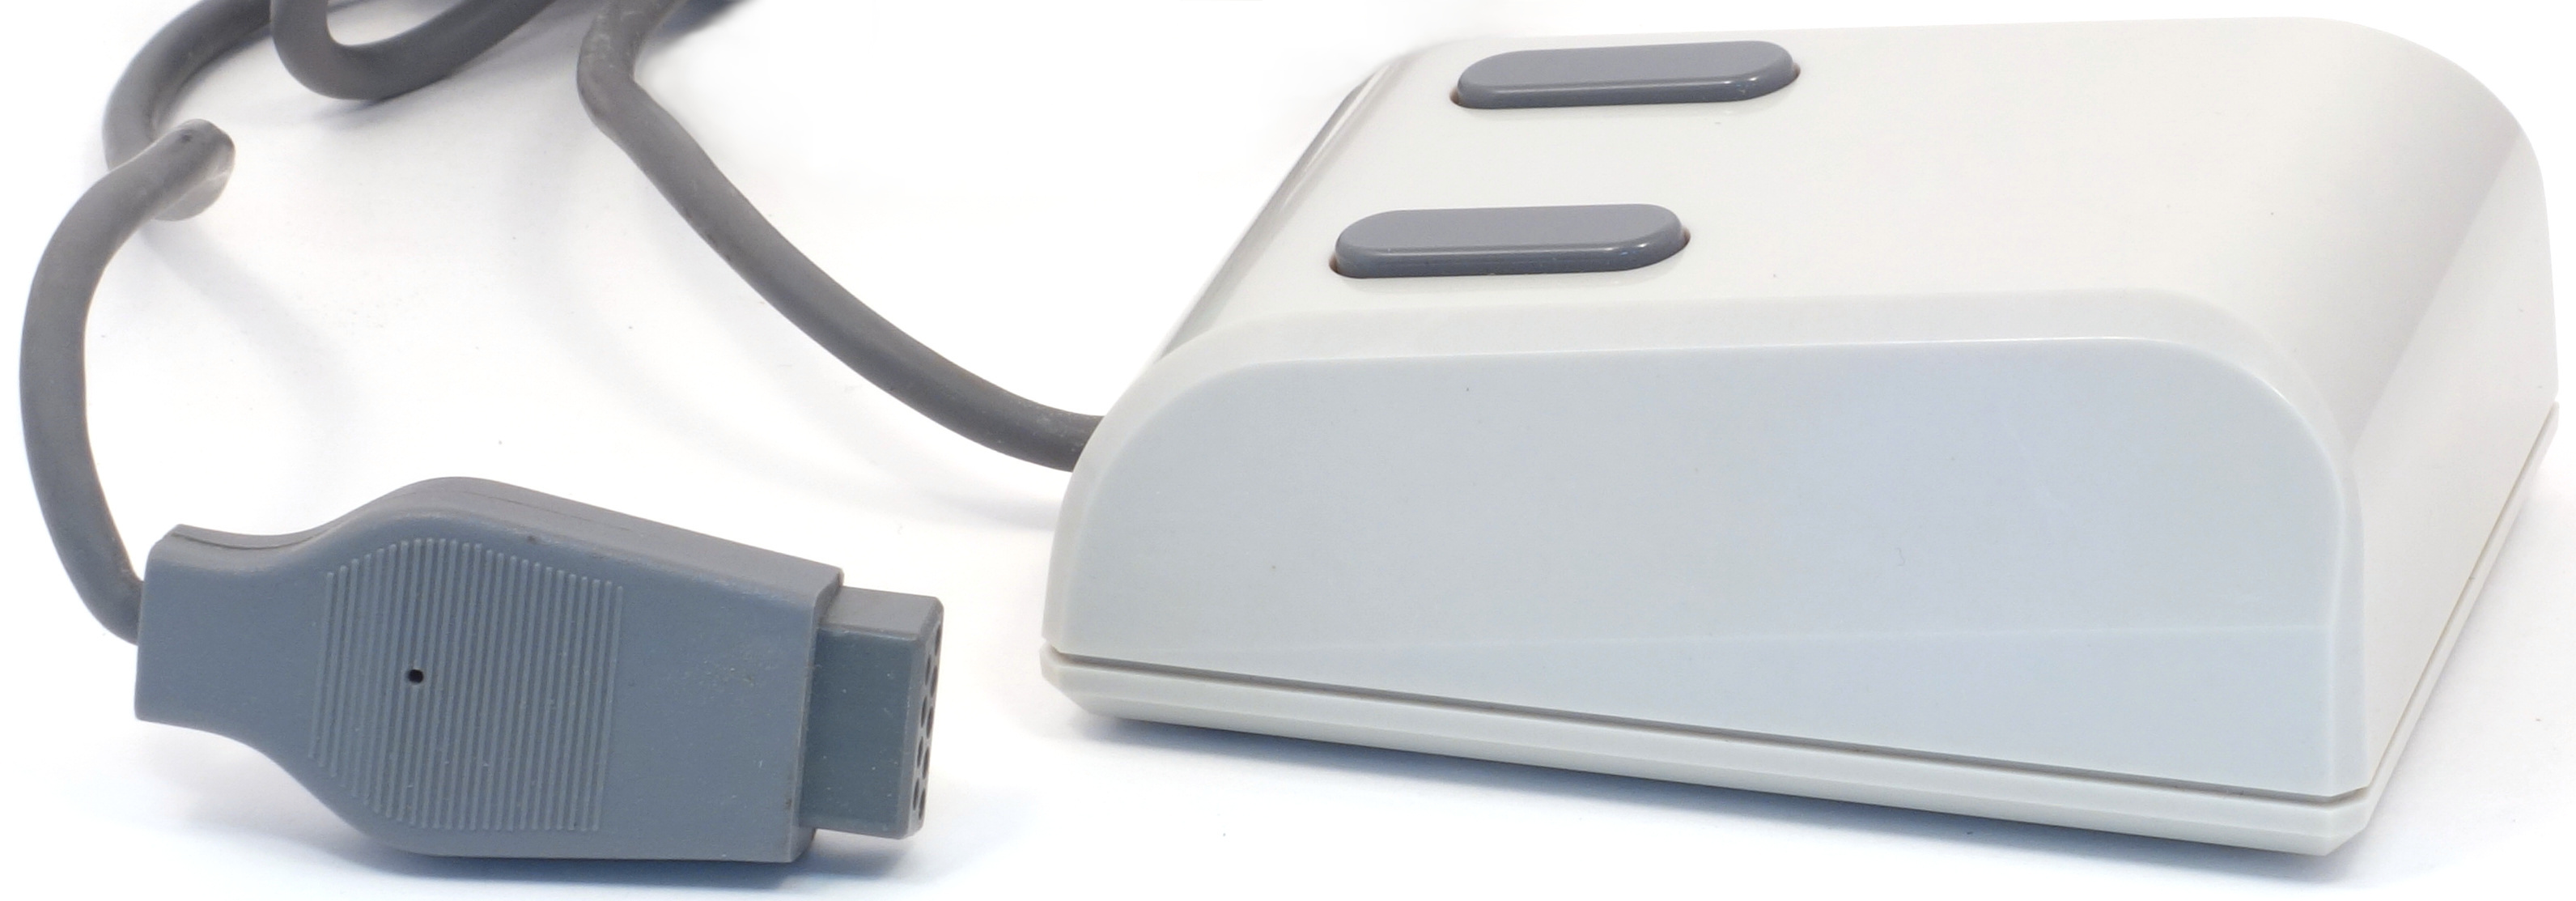
\includegraphics[scale=0.7]{1986_commodore_c300_mouse/cmnirm_30.jpg}
    \caption{Commodore C300 Mouse}
    \label{fig:C300Pic}
\end{figure}

According to the accompanying description, this mouse has two modes of operation: joystick mode and proportional mode. The operating mode is determined when the computer is turned on: the pressed right mouse button turns on the joystick mode, otherwise (by default) the mouse works in proportional mode. In joystick mode, the left mouse button is used as the joystick button, and the right button is equivalent to moving the joystick up. Joystick mode allows you to use the mouse with any joystick-compatible software, and also acts as a "fallback" in case the software you are using does not support proportional mode.

\begin{figure}[h]
    \centering
    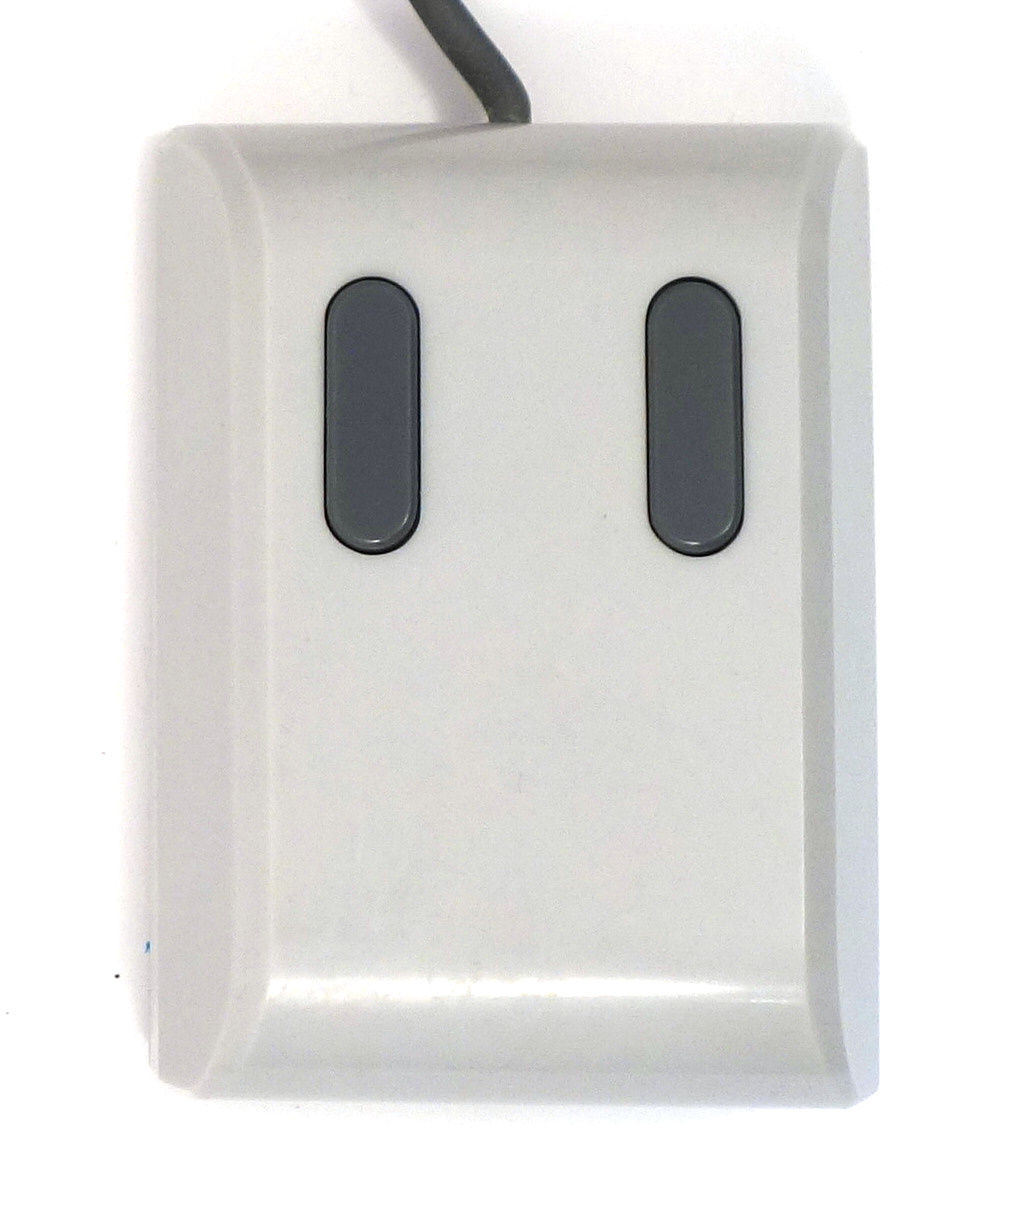
\includegraphics[scale=0.75]{1986_commodore_c300_mouse/3verh_60.jpg}
    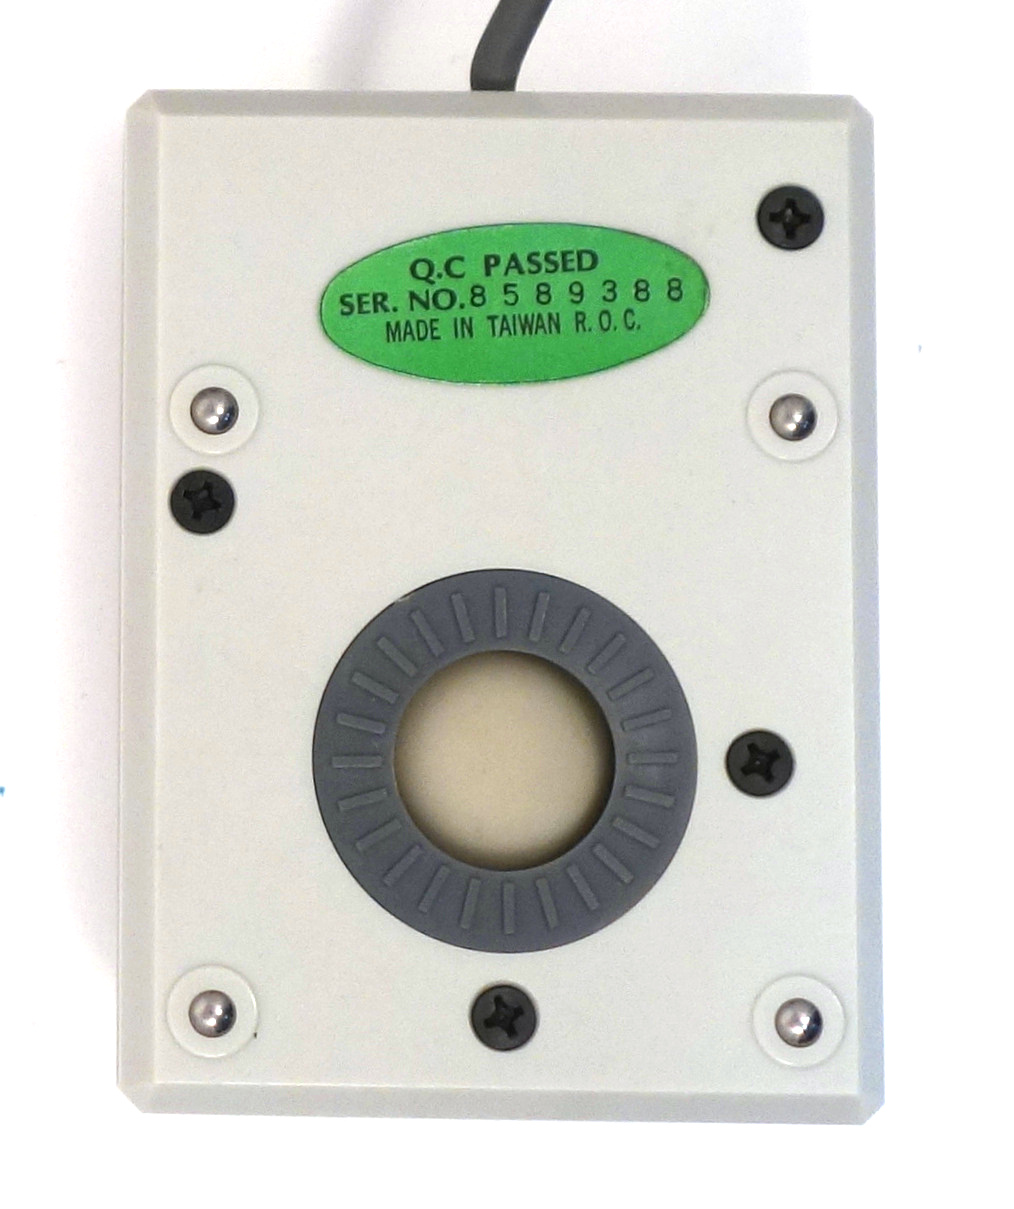
\includegraphics[scale=0.75]{1986_commodore_c300_mouse/3niz_60.jpg}
    \caption{Commodore C300 Mouse, top and bottom views}
    \label{fig:C300TopAndBottom}
\end{figure}

As you can see in figure \ref{fig:C300TopAndBottom}, the smooth glide of the mouse over the work surface is provided not by low-resistance fabric pads or plastic <<feet>>, but by four small-diameter metal balls located in additional holes on the bottom side of the case, which rotate freely when moving (a solution typical for a number of mechanical mice of the 80s, produced before the change in the standard design, aimed at reducing the cost of products).

\begin{figure}[h]
    \centering
    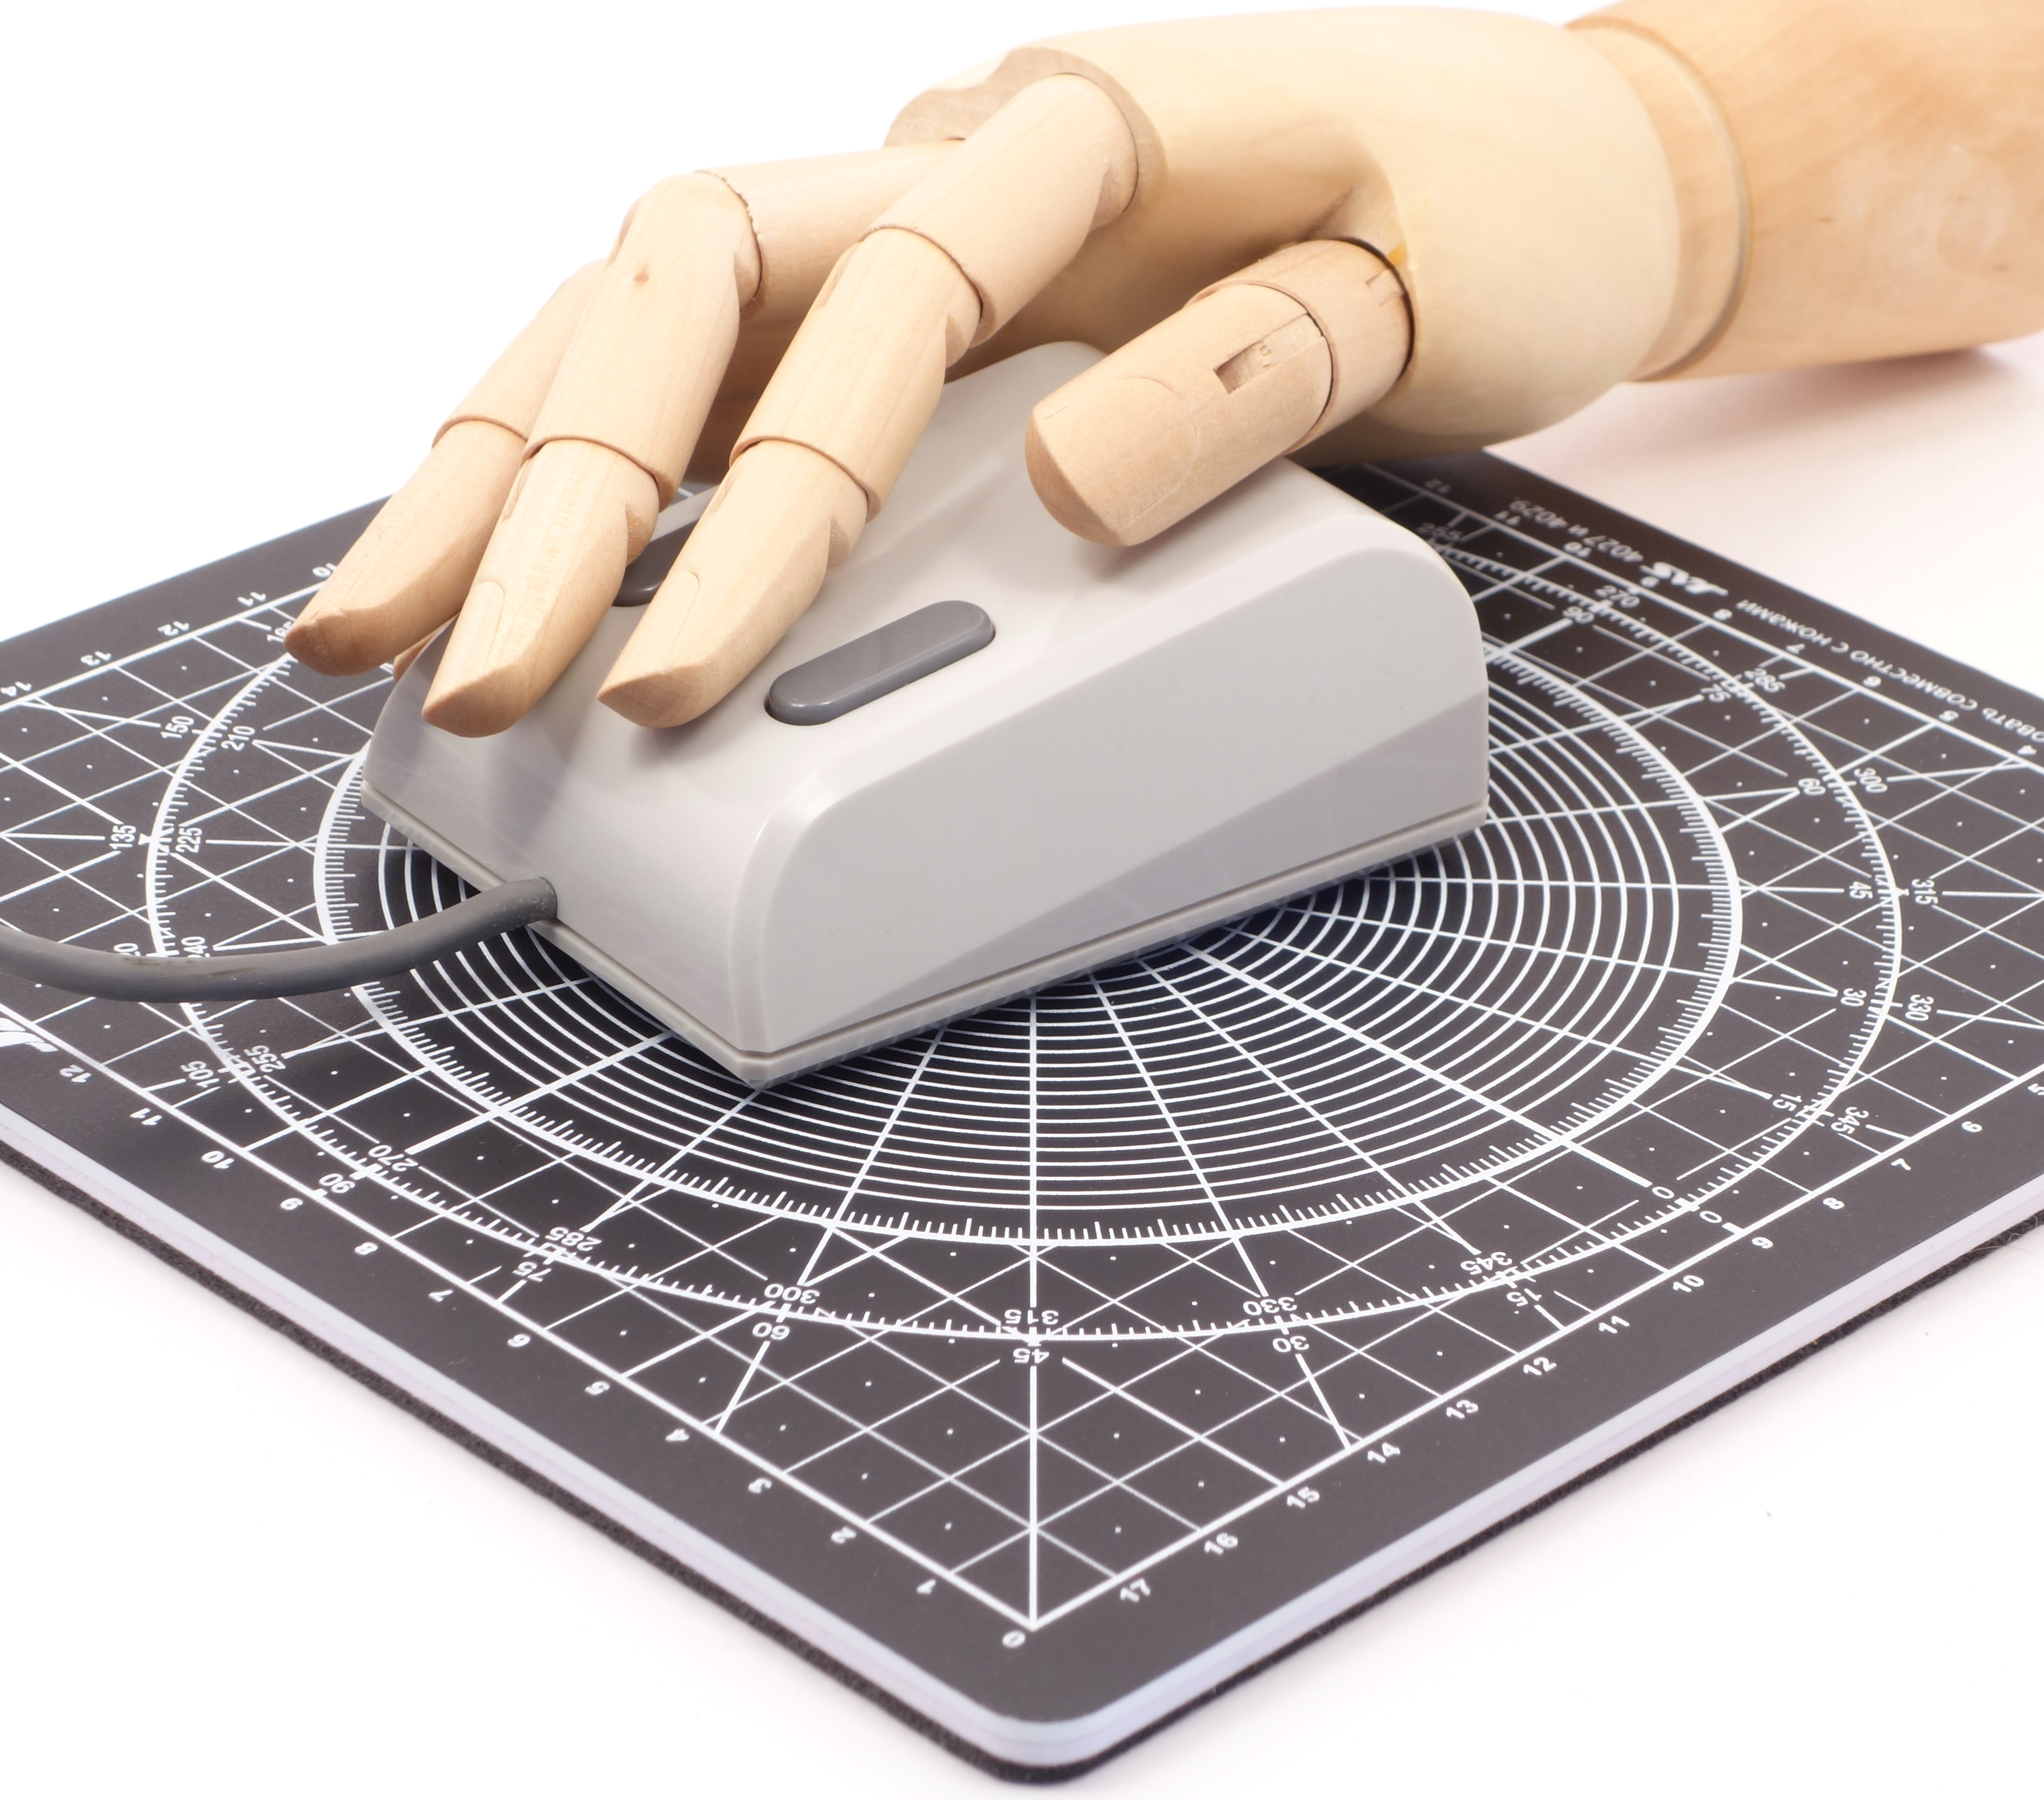
\includegraphics[scale=0.35]{1986_commodore_c300_mouse/cmruka_30.jpg}
    \caption{Commodore C300 Mouse with a human hand model}
    \label{fig:C300Hand}
\end{figure}

\begin{figure}[h]
    \centering
    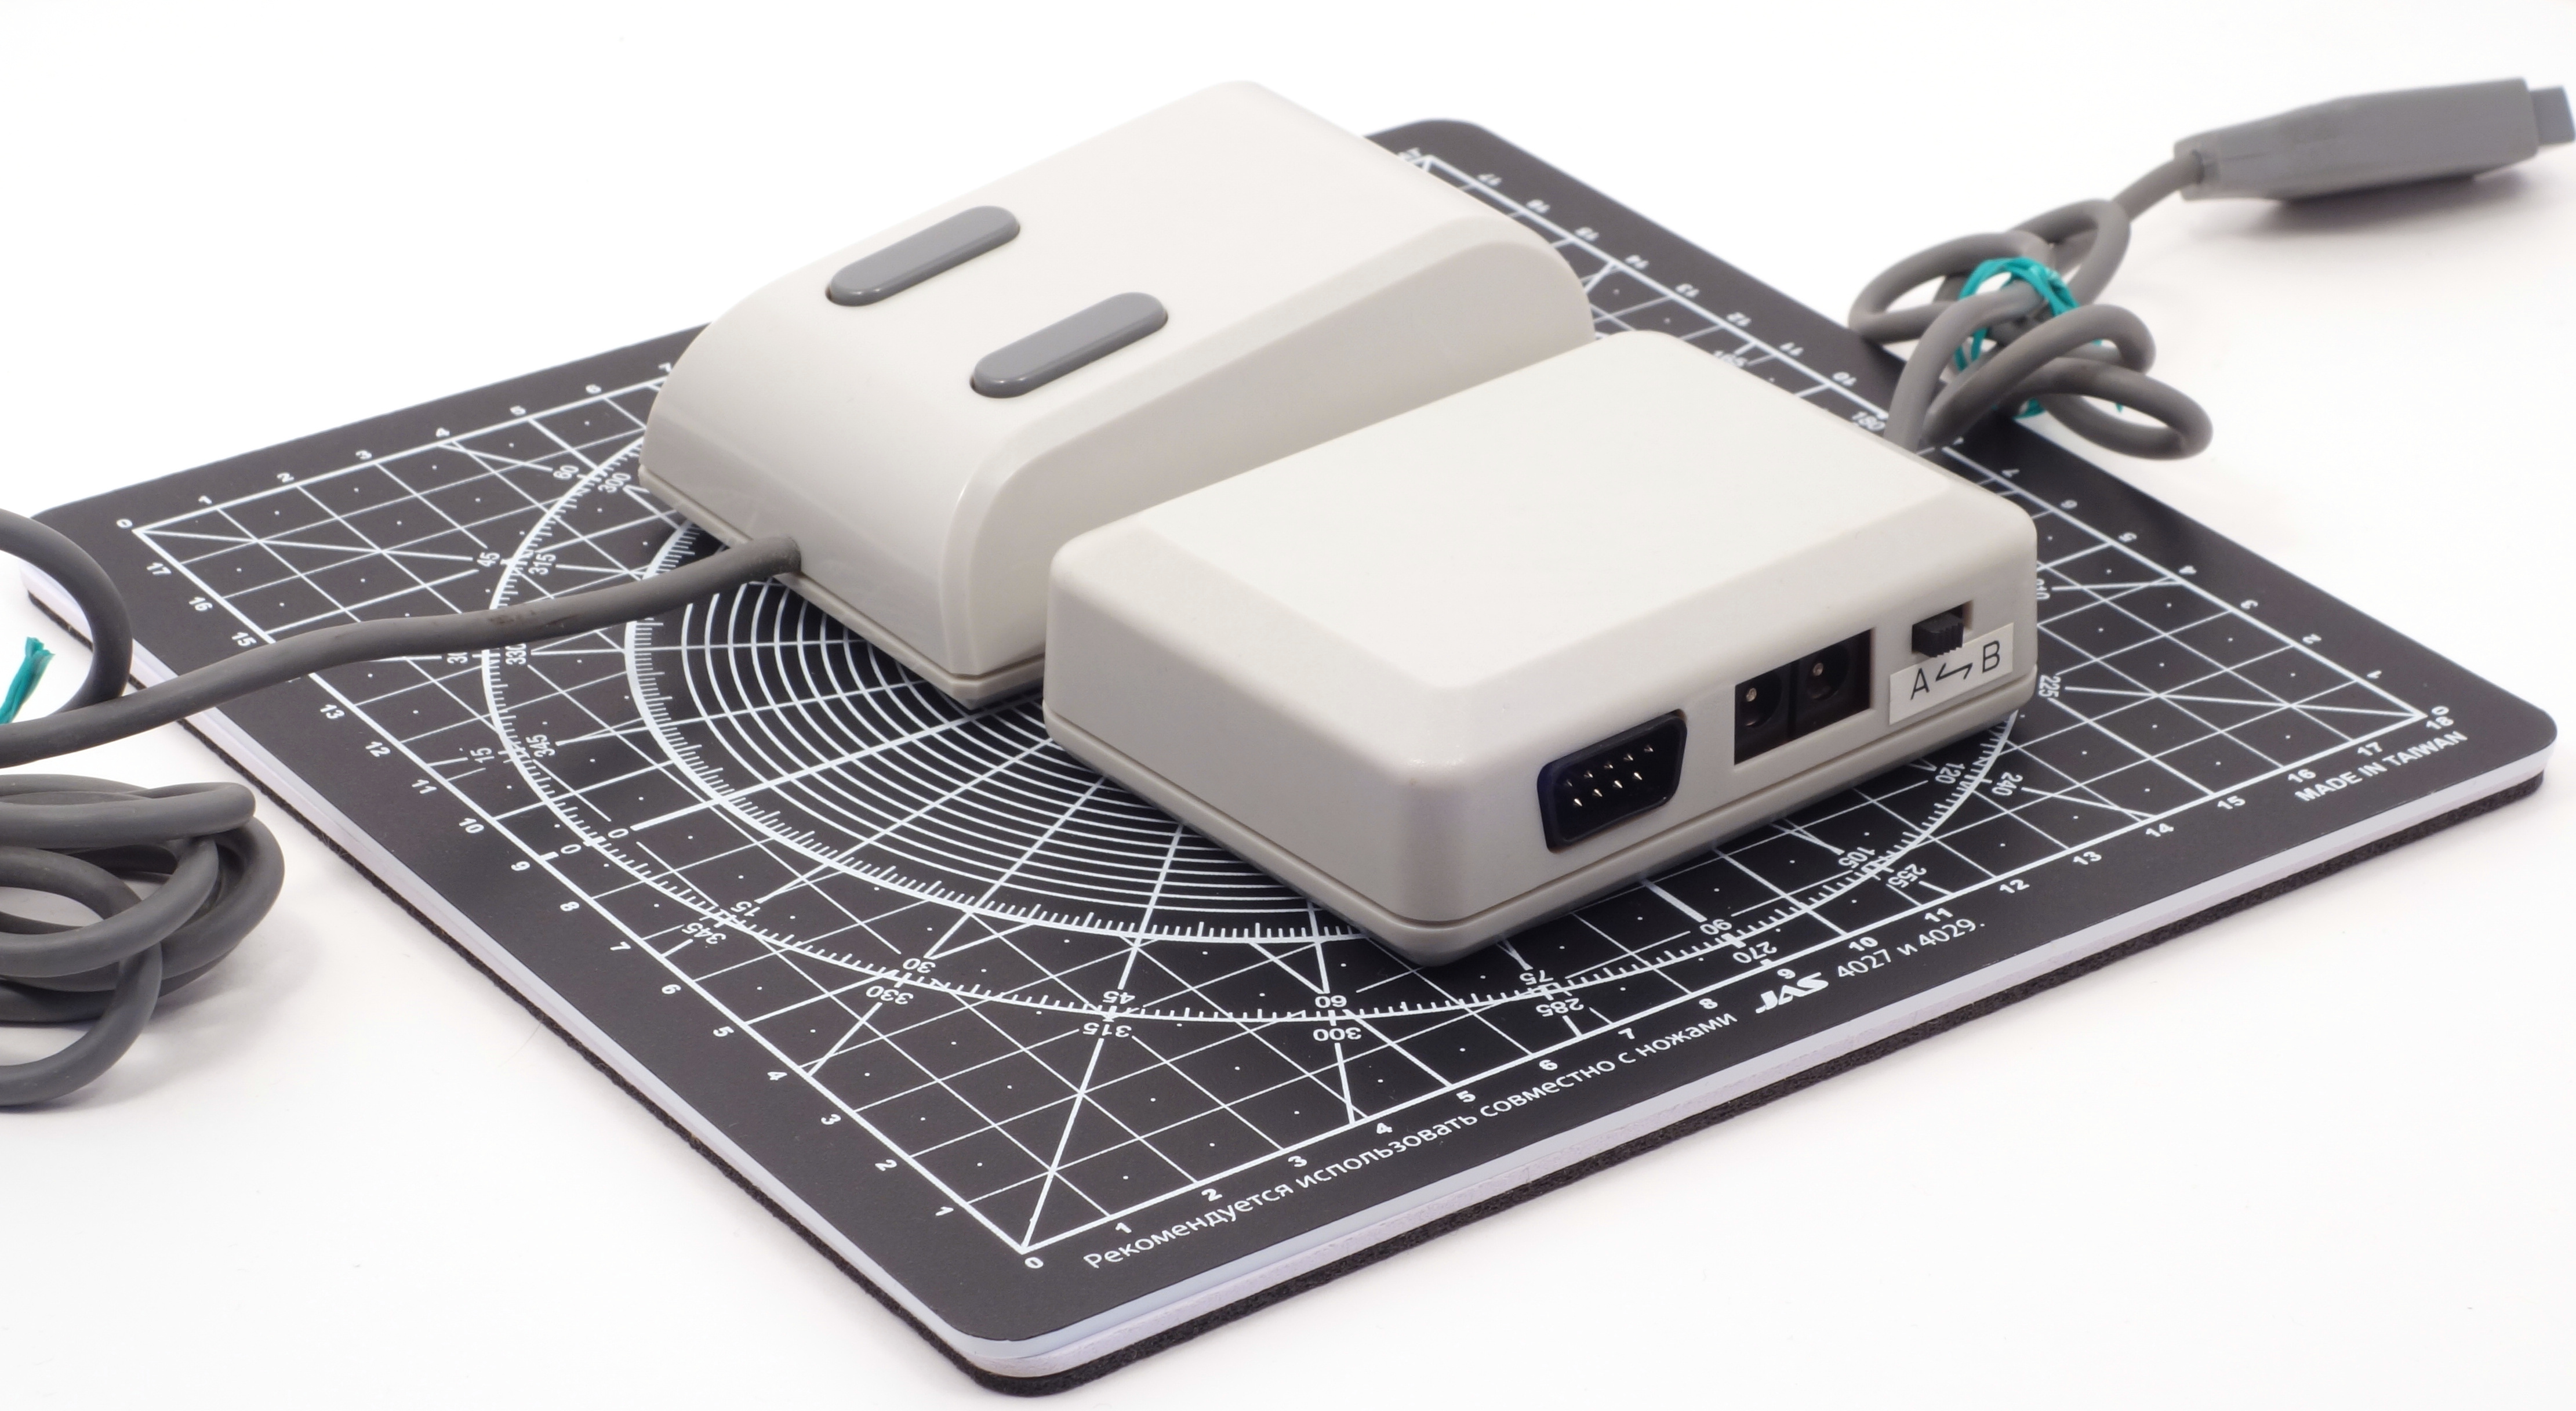
\includegraphics[scale=0.3]{1986_commodore_c300_mouse/cmblock_30.jpg}
    \caption{Commodore C300 mouse and adapter on a graduated pad with a grid step of 1~cm}
    \label{fig:C300Block}
\end{figure}

\begin{figure}[h]
    \centering
    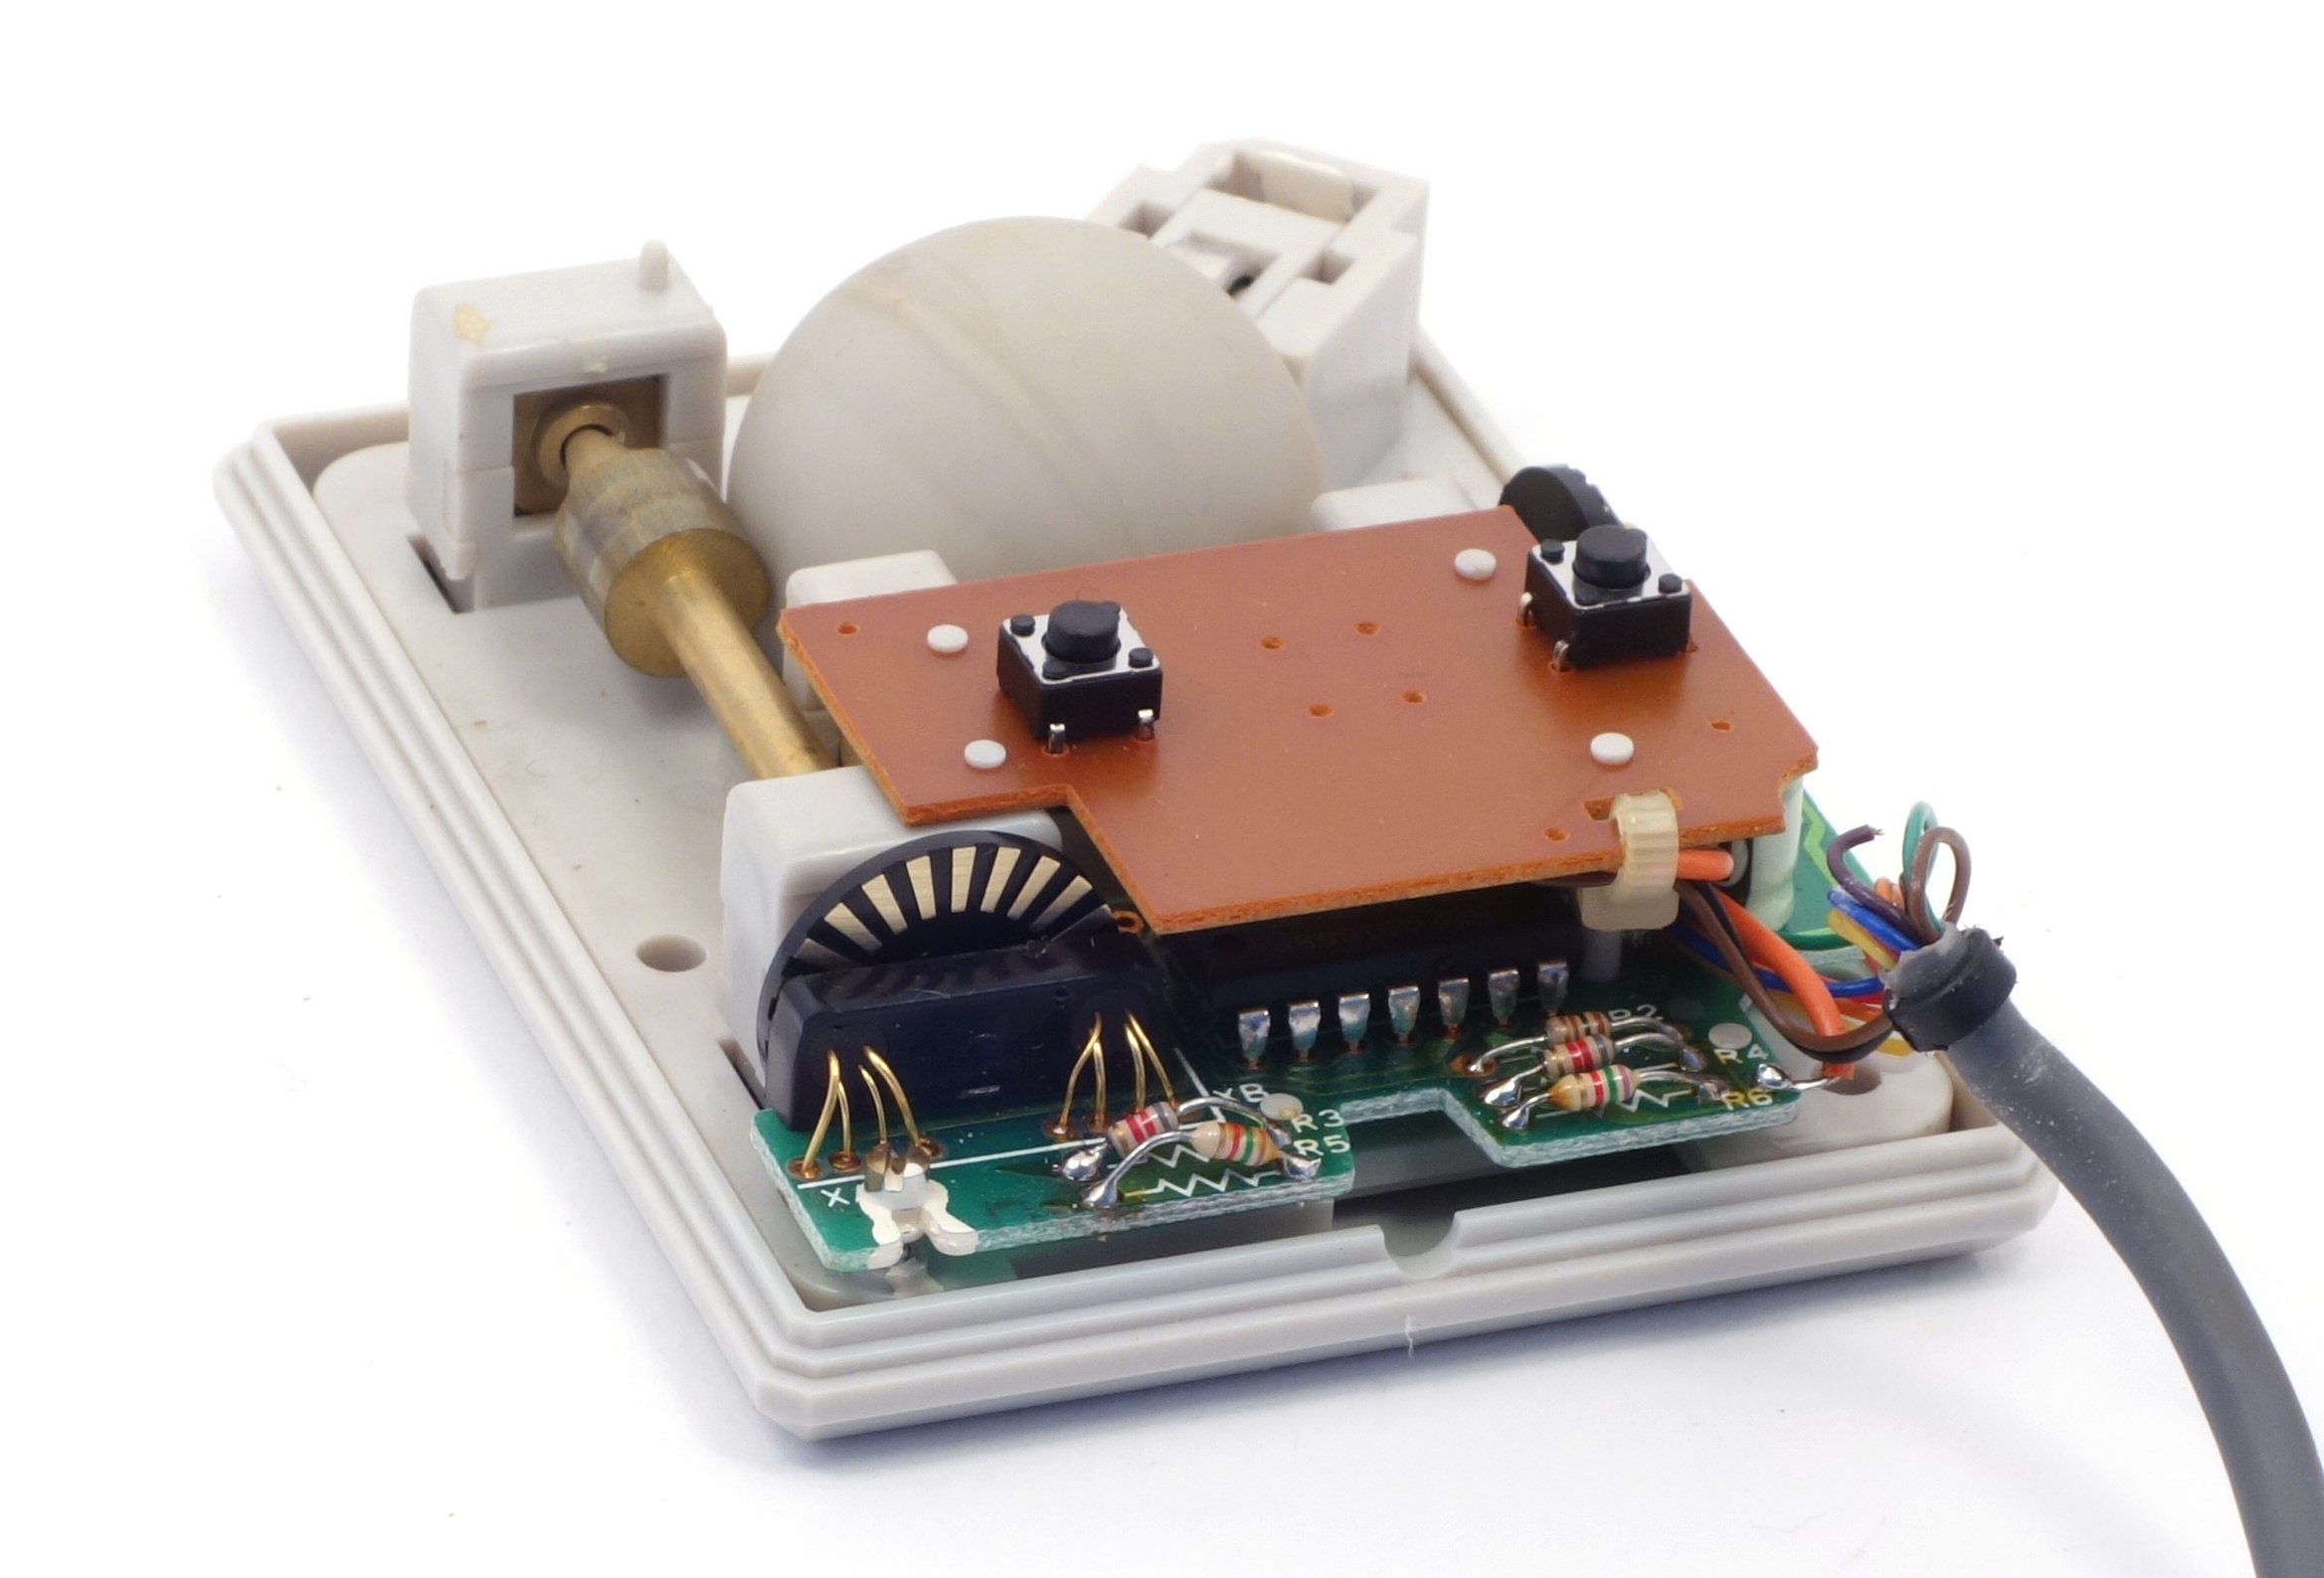
\includegraphics[scale=0.7]{1986_commodore_c300_mouse/cm4raz_30.jpg}
%    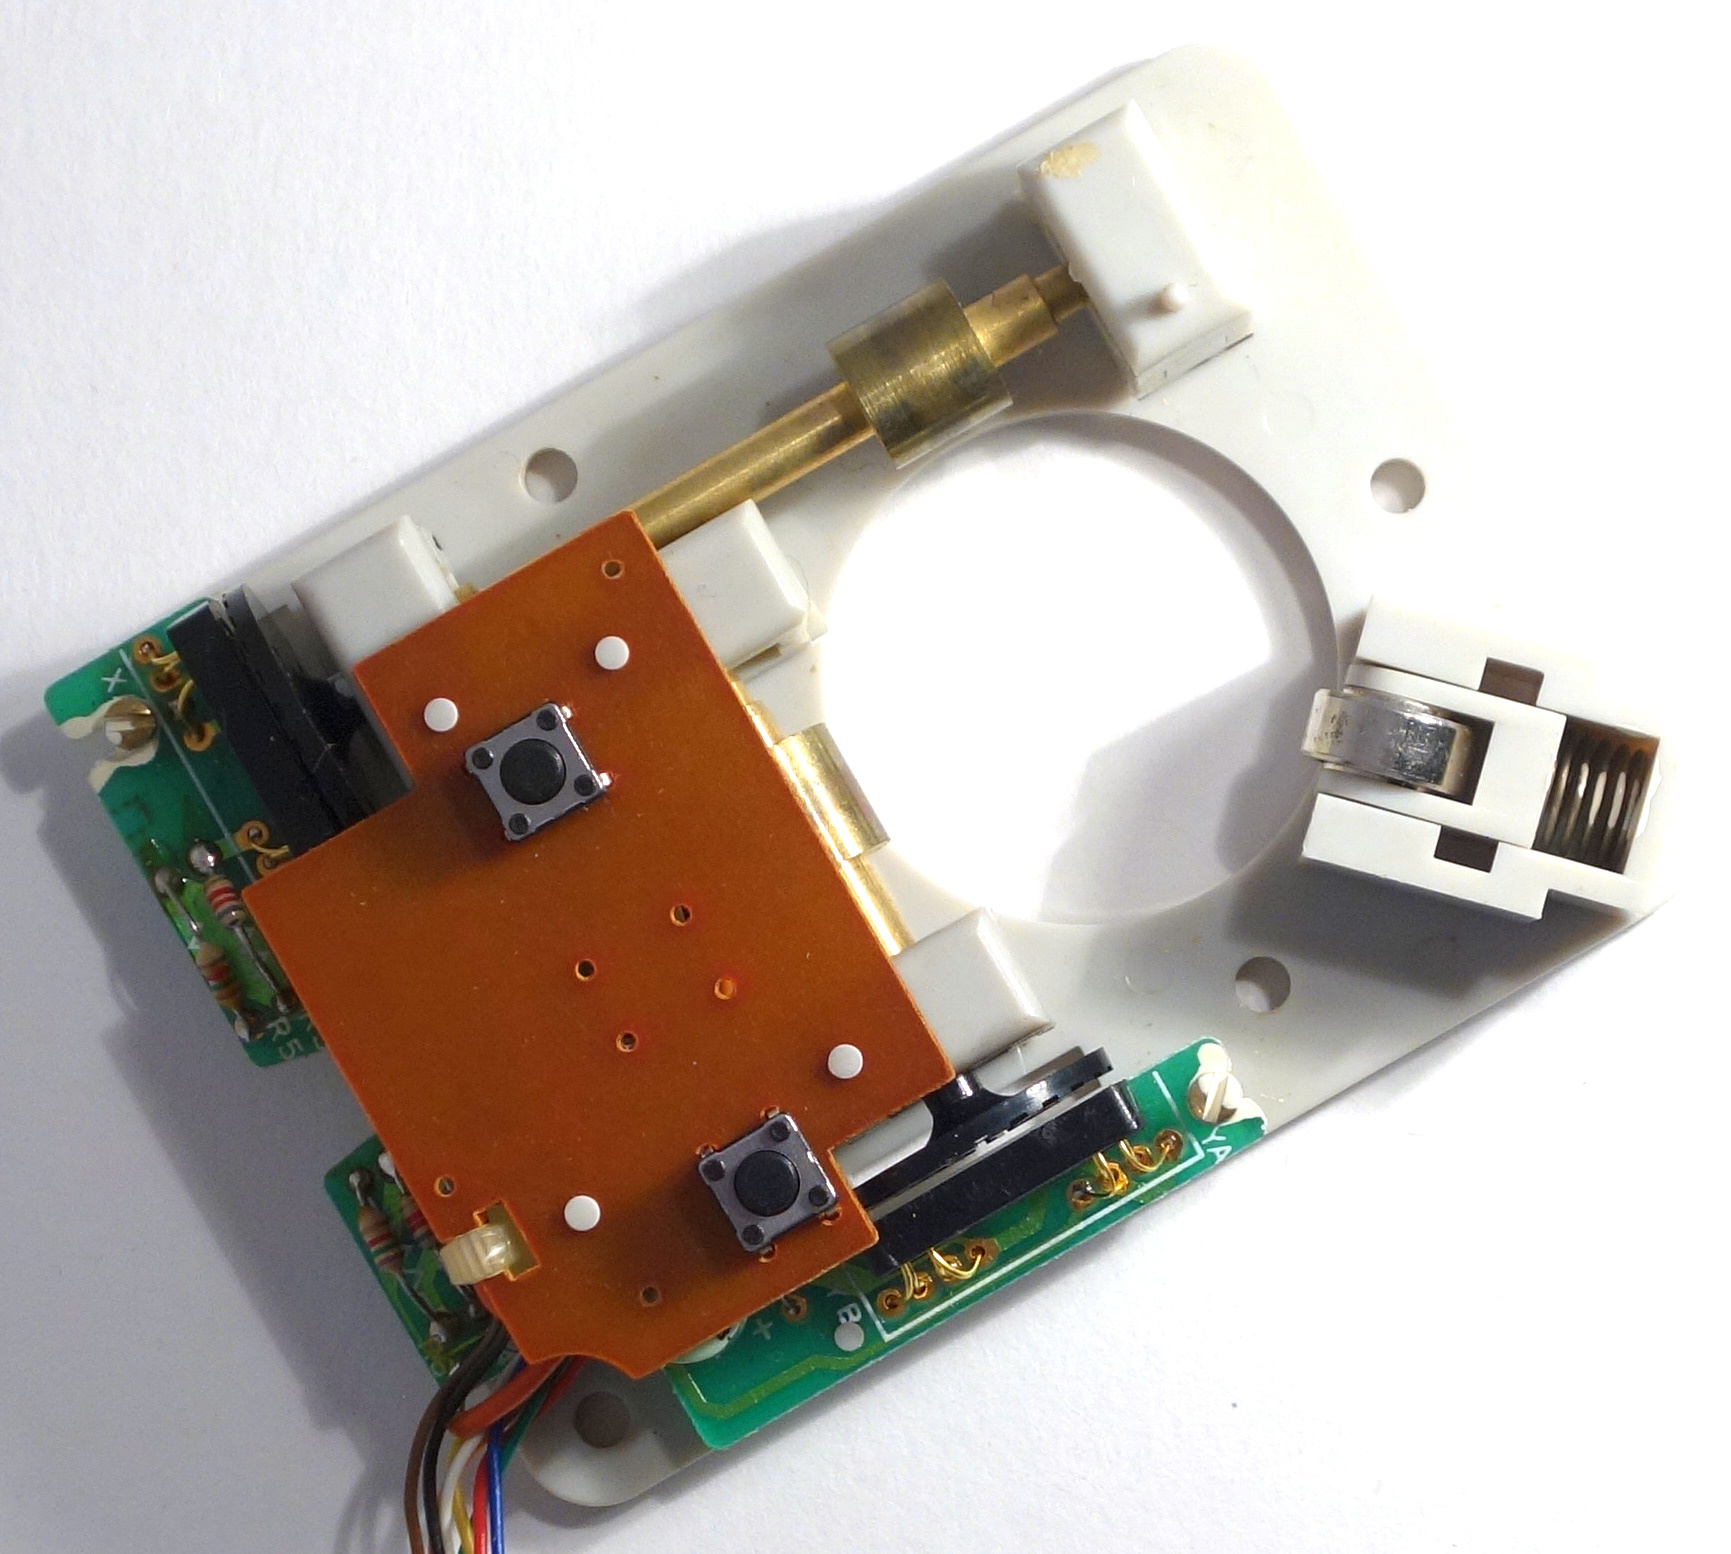
\includegraphics[scale=0.7]{1986_commodore_c300_mouse/cm41raz_30.jpg}
    \caption{Commodore C300 Mouse disassembled}
    \label{fig:C300Inside}
\end{figure}

Mouse internals are shown on figure \ref{fig:C300Inside}. The design is quite unusual: this is an original optomechanical pointing device with a non-standard optical interrupter. Instead of passing the disk between the light source and the optical detector, the LED and the photodiode are located on the same side of the disk, and the disk itself is Solid. Instead of slots, it used the radial metal strips reflecting light, while the black matte material of the disk itself scatters it, causing the absence of a signal on the photo receiver. In electrical terms, such a design does not differ from other opto-mechanical mice, but visually resembles a disk of contact encoder (in which the mechanical contact of the brushes with the surface of the disk occurs: there is an electrical contact at the time of the passing of a metal radial strip, and there is no contact when the brush is between the stripes).

Of course, such a solution is not cheap in comparison with a traditional scheme that uses a plastic disk with slots without metal.

\begin{thebibliography}{9}
\bibitem {c64wiki} Mouse -- C64-Wiki \url{https://www.c64-wiki.com/wiki/Mouse}
\bibitem {SinclairUser} Kempston mouse // Sinclair User, Iss. 56, November 1986. -- p. 29. \url{https://worldofspectrum.org/archive/magazines/sinclair-user/56/0/1986/11/0}
\end{thebibliography}
\end{document}

\documentclass[11pt, a4paper]{article}
\usepackage{pdfpages}
\usepackage{parallel}
\usepackage[T2A]{fontenc}
\usepackage{ucs}
\usepackage[utf8x]{inputenc}
\usepackage[polish,english,russian]{babel}
\usepackage{hyperref}
\usepackage{rotating}
\usepackage[inner=2cm,top=1.8cm,outer=2cm,bottom=2.3cm,nohead]{geometry}
\usepackage{listings}
\usepackage{graphicx}
\usepackage{wrapfig}
\usepackage{longtable}
\usepackage{indentfirst}
\usepackage{array}
\usepackage{tikzsymbols}
\usepackage{soul}
\usepackage[ruled,vlined]{algorithm2e}
%\counterwithout{figure}{section} 

\usepackage{url}
\makeatletter
\g@addto@macro{\UrlBreaks}{\UrlOrds}
\makeatother

\newcolumntype{P}[1]{>{\raggedright\arraybackslash}p{#1}}
\frenchspacing
\usepackage{fixltx2e} %text sub- and superscripts
\usepackage{icomma} % коскі ў матэматычным рэжыме
\PreloadUnicodePage{4}

\newcommand{\longpage}{\enlargethispage{\baselineskip}}
\newcommand{\shortpage}{\enlargethispage{-\baselineskip}}

\def\switchlang#1{\expandafter\csname switchlang#1\endcsname}
\def\switchlangbe{
\let\saverefname=\refname%
\def\refname{Літаратура}%
\def\figurename{Іл.}%
}
\def\switchlangen{
\let\saverefname=\refname%
\def\refname{References}%
\def\figurename{Fig.}%
}
\def\switchlangru{
\let\saverefname=\refname%
\let\savefigurename=\figurename%
\def\refname{Литература}%
\def\figurename{Рис.}%
}

\hyphenation{admi-ni-stra-tive}
\hyphenation{ex-pe-ri-ence}
\hyphenation{fle-xi-bi-li-ty}
\hyphenation{Py-thon}
\hyphenation{ma-the-ma-ti-cal}
\hyphenation{re-ported}
\hyphenation{imp-le-menta-tions}
\hyphenation{pro-vides}
\hyphenation{en-gi-neering}
\hyphenation{com-pa-ti-bi-li-ty}
\hyphenation{im-pos-sible}
\hyphenation{desk-top}
\hyphenation{elec-tro-nic}
\hyphenation{com-pa-ny}
\hyphenation{de-ve-lop-ment}
\hyphenation{de-ve-loping}
\hyphenation{de-ve-lop}
\hyphenation{da-ta-ba-se}
\hyphenation{plat-forms}
\hyphenation{or-ga-ni-za-tion}
\hyphenation{pro-gramming}
\hyphenation{in-stru-ments}
\hyphenation{Li-nux}
\hyphenation{sour-ce}
\hyphenation{en-vi-ron-ment}
\hyphenation{Te-le-pathy}
\hyphenation{Li-nux-ov-ka}
\hyphenation{Open-BSD}
\hyphenation{Free-BSD}
\hyphenation{men-ti-on-ed}
\hyphenation{app-li-ca-tion}

\def\progref!#1!{\texttt{#1}}
\renewcommand{\arraystretch}{2} %Іначай формулы ў матрыцы зліпаюцца з лініямі
\usepackage{array}

\def\interview #1 (#2), #3, #4, #5\par{

\section[#1, #3, #4]{#1 -- #3, #4}
\def\qname{LVEE}
\def\aname{#1}
\def\q ##1\par{{\noindent \bf \qname: ##1 }\par}
\def\a{{\noindent \bf \aname: } \def\qname{L}\def\aname{#2}}
}

\def\interview* #1 (#2), #3, #4, #5\par{

\section*{#1\\{\small\rm #3, #4. #5}}
\ifx\ParallelWhichBox\undefined%
    \addcontentsline{toc}{section}{#1, #3, #4}%
\else%
\ifnum\ParallelWhichBox=0%
    \addcontentsline{toc}{section}{#1, #3, #4}%
\fi\fi%

\def\qname{LVEE}
\def\aname{#1}
\def\q ##1\par{{\noindent \bf \qname: ##1 }\par}
\def\a{{\noindent \bf \aname: } \def\qname{L}\def\aname{#2}}
}

\newcommand{\interviewfooter}[1]{
\vskip 1em
\noindent \textit{#1}
}


\begin{document}

\title{1986 "--- American Mouse}
\date{}
\maketitle

In 1986, the American Computer and Peripheral company released the American 286 desktop computer, based on the i80286 processor \cite{adv}, and equipped with a mouse called the American Mouse (figure \ref{fig:AmericanPic}). The price of the device in a separate sale was \$125 \cite{review}.

\begin{figure}[h]
    \centering
    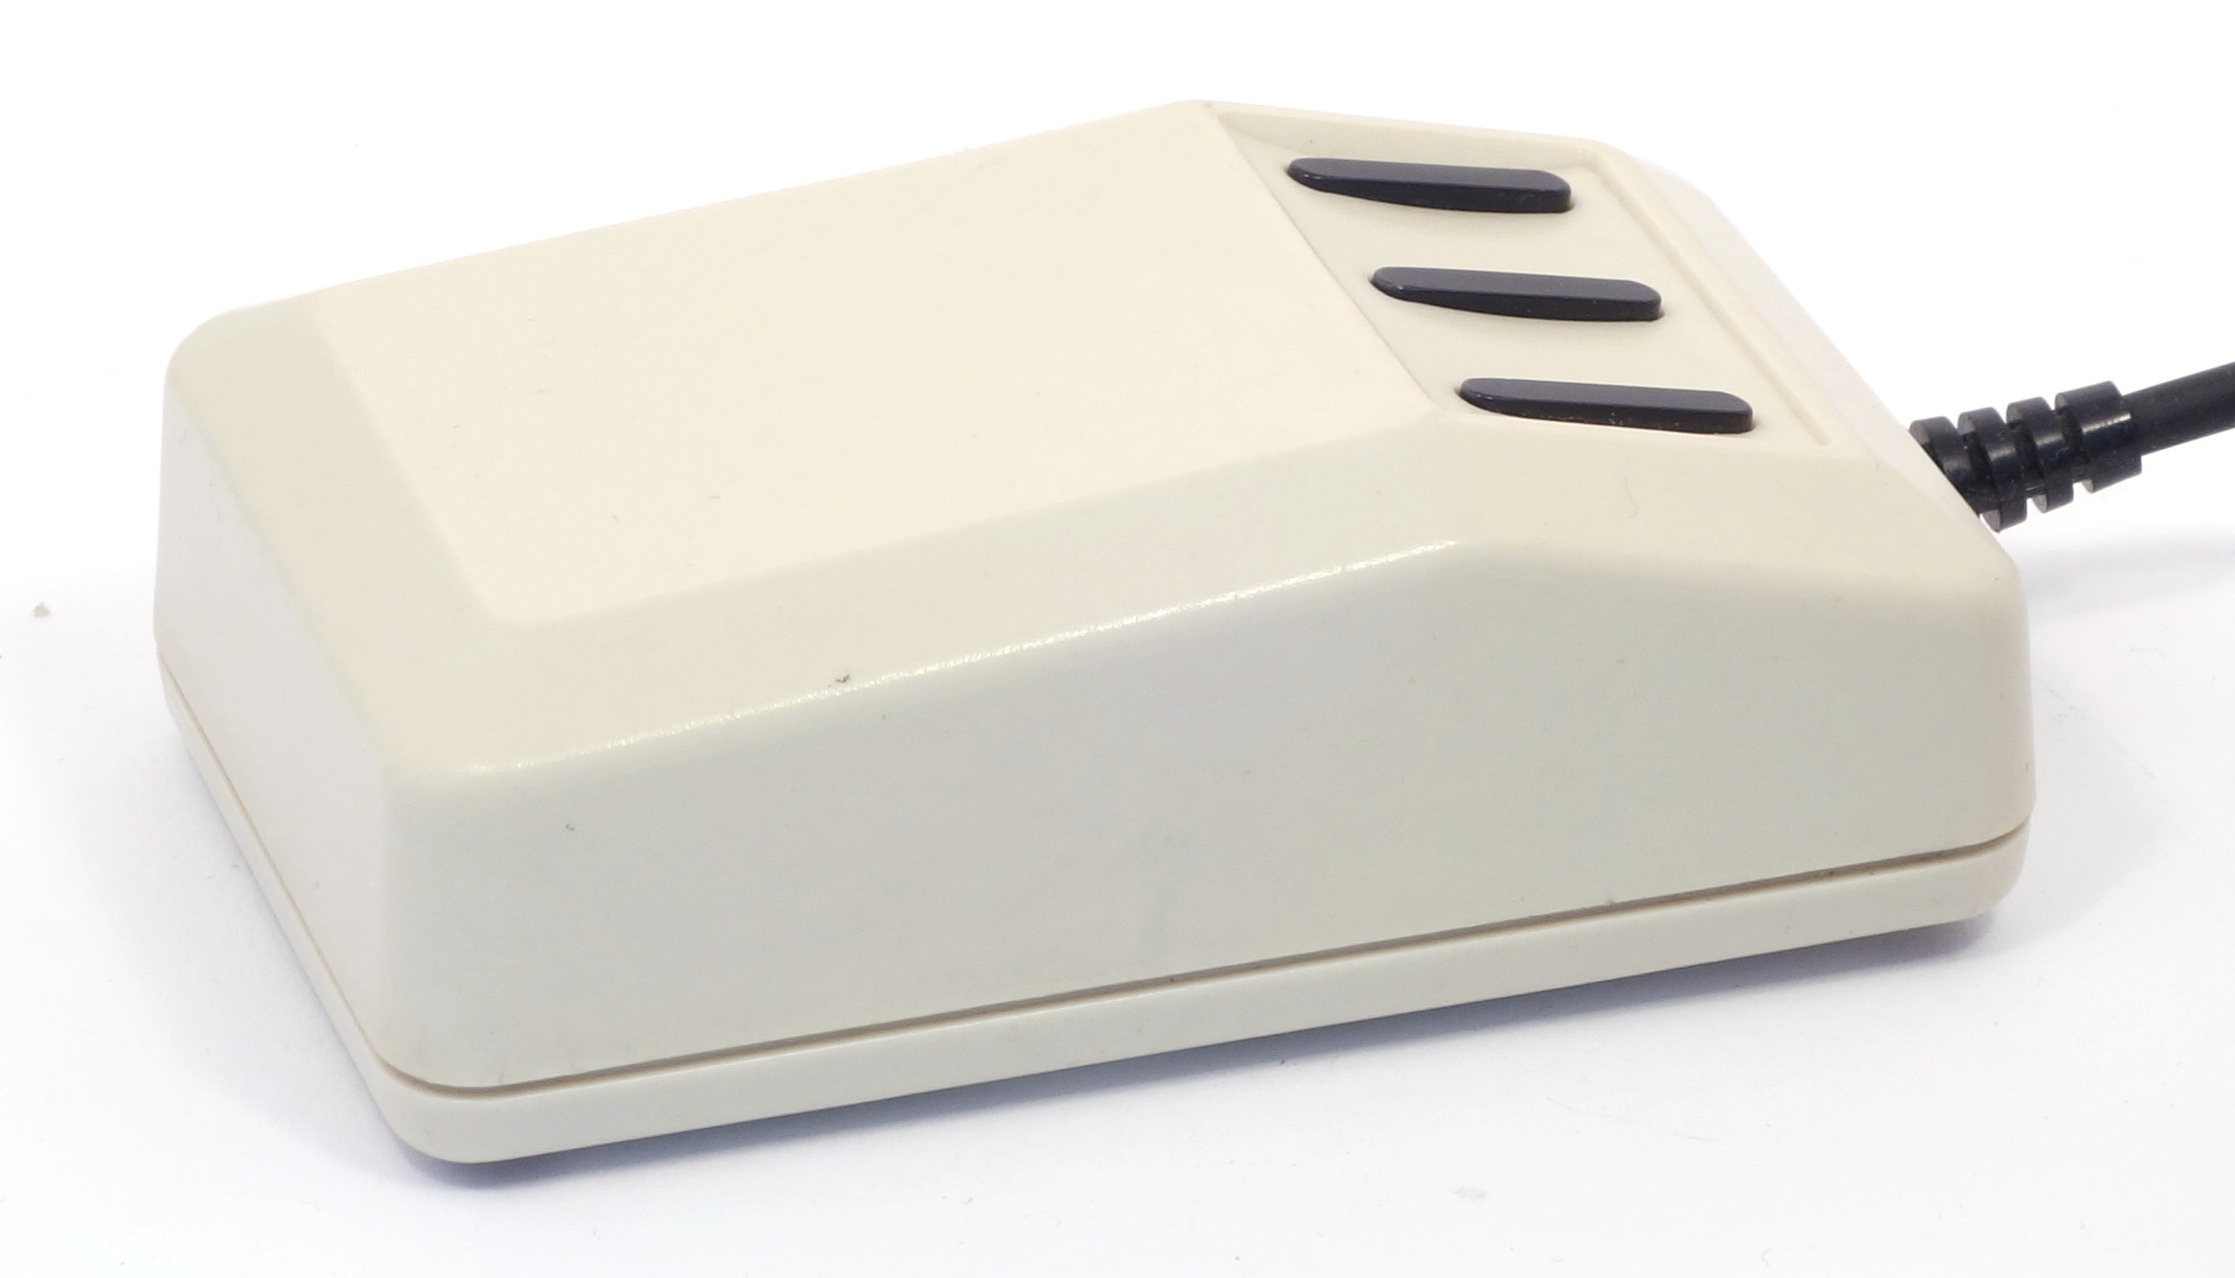
\includegraphics[scale=0.7]{1986_american_mouse/pic_30.jpg}
    \caption{American Mouse}
    \label{fig:AmericanPic}
\end{figure}

A notch on the slightly slanted front of the mouse cover houses three phenomenally narrow buttons. Massive switches located under the buttons forced developers to use an asymmetrical layout of the mouse cable that runs between the left and middle buttons (figure \ref{AmericanTopAndBottom}). The underside of the housing contains a removable ring to remove the ball and clean the mouse. There are no inscriptions or emblems on the case.

\begin{figure}[h]
    \centering
    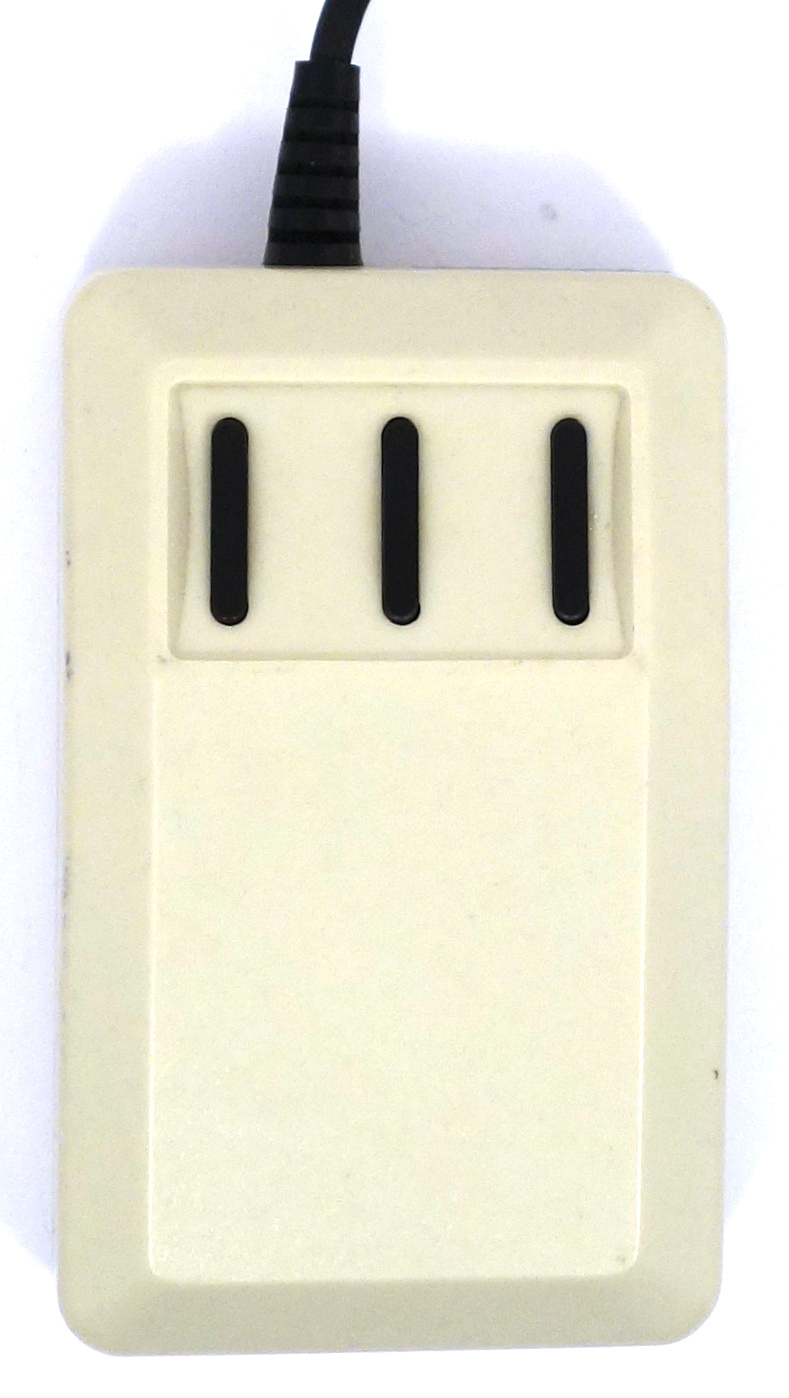
\includegraphics[scale=0.7]{1986_american_mouse/top_60.jpg}
    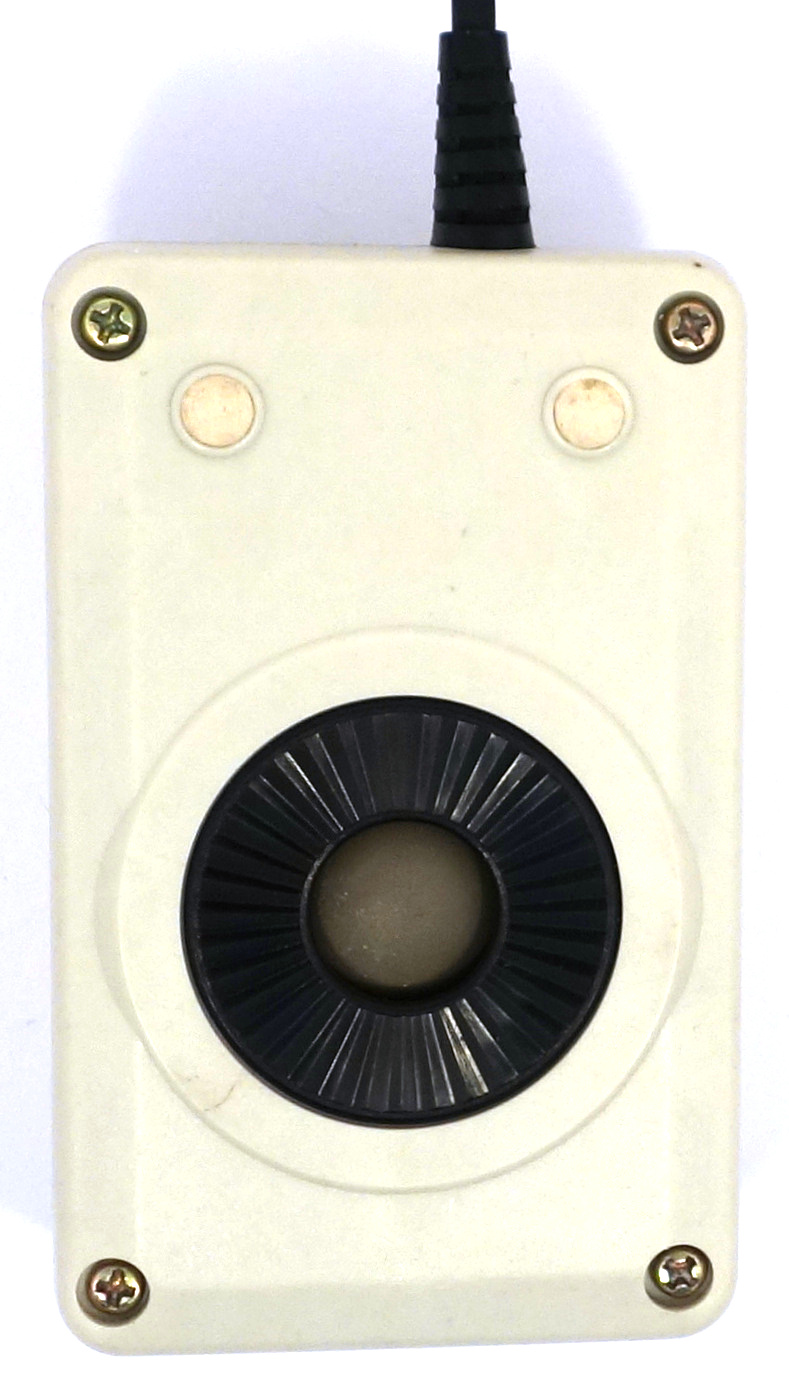
\includegraphics[scale=0.7]{1986_american_mouse/bottom_60.jpg}
    \caption{American Mouse, top and bottom views}
    \label{AmericanTopAndBottom}
\end{figure}

In term of size, the manipulator is an optomechanical cursor control device typical of the 1980s (figure \ref{fig:AmericanSize}).

\begin{figure}[h]
    \centering
    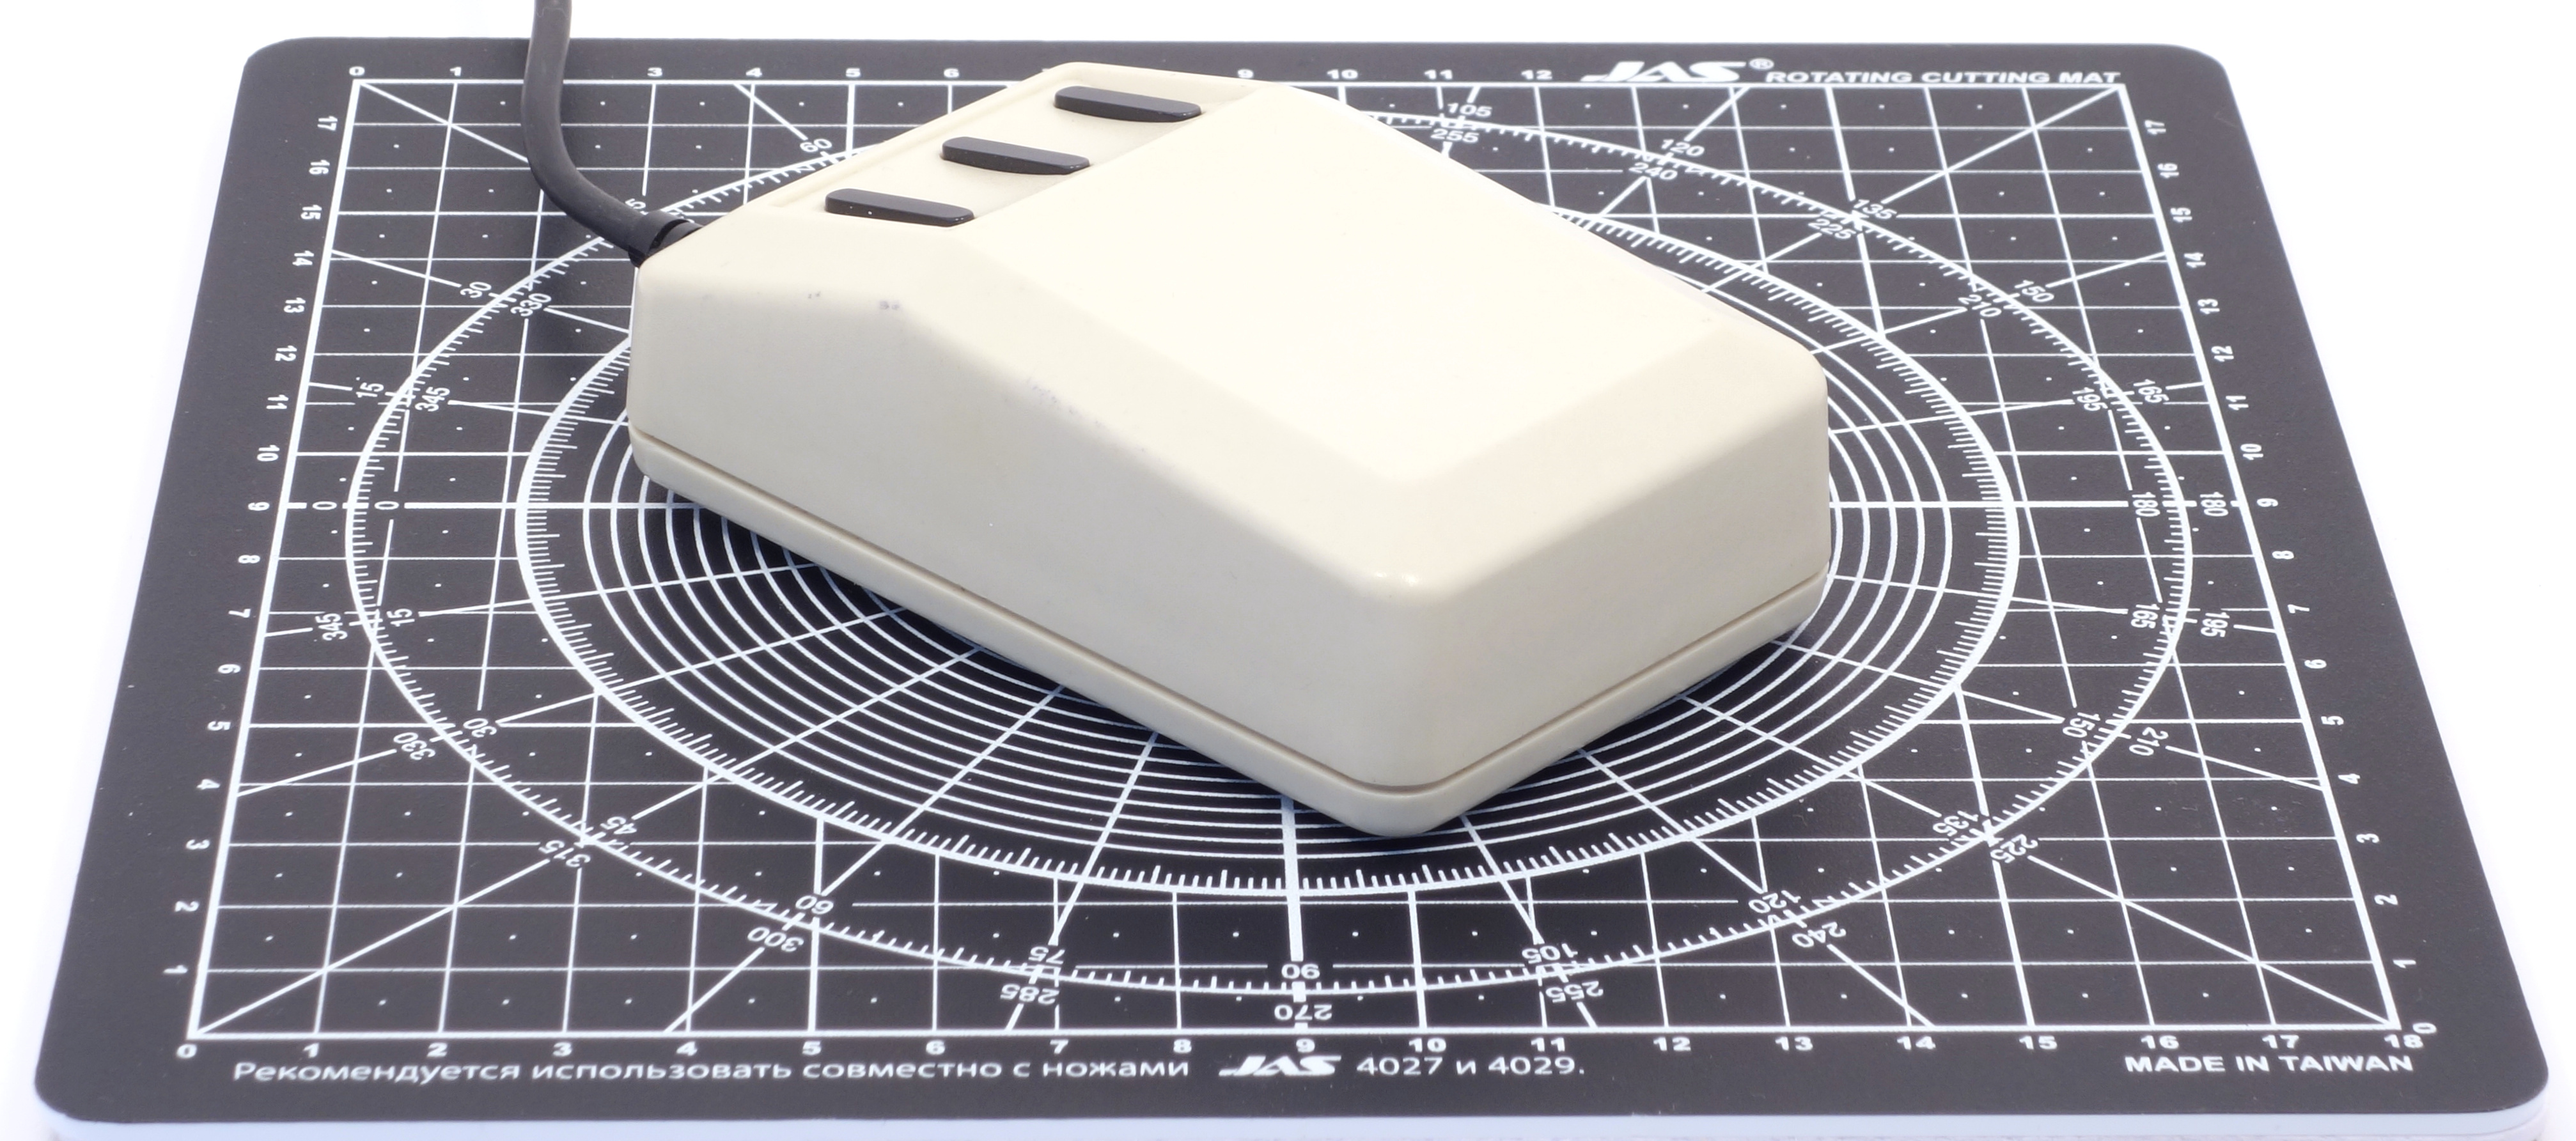
\includegraphics[scale=0.5]{1986_american_mouse/size_30.jpg}
    \caption{Изображение American Mouse on a graduated pad with a grid step of 1~cm}
    \label{fig:AmericanSize}
\end{figure}

The exterior of the American Mouse has a clear industrial design. At the same time, the angular body was equipped with beveled edges to provide a more comfortable palm position; however, the need to press extremely narrow buttons that cut into the fingertips negates the ergonomic efforts of the developers and allows us to rank this manipulator among the most questionable devices in the design (figure \ref{fig:AmericanHand}).

\begin{figure}[h]
    \centering
    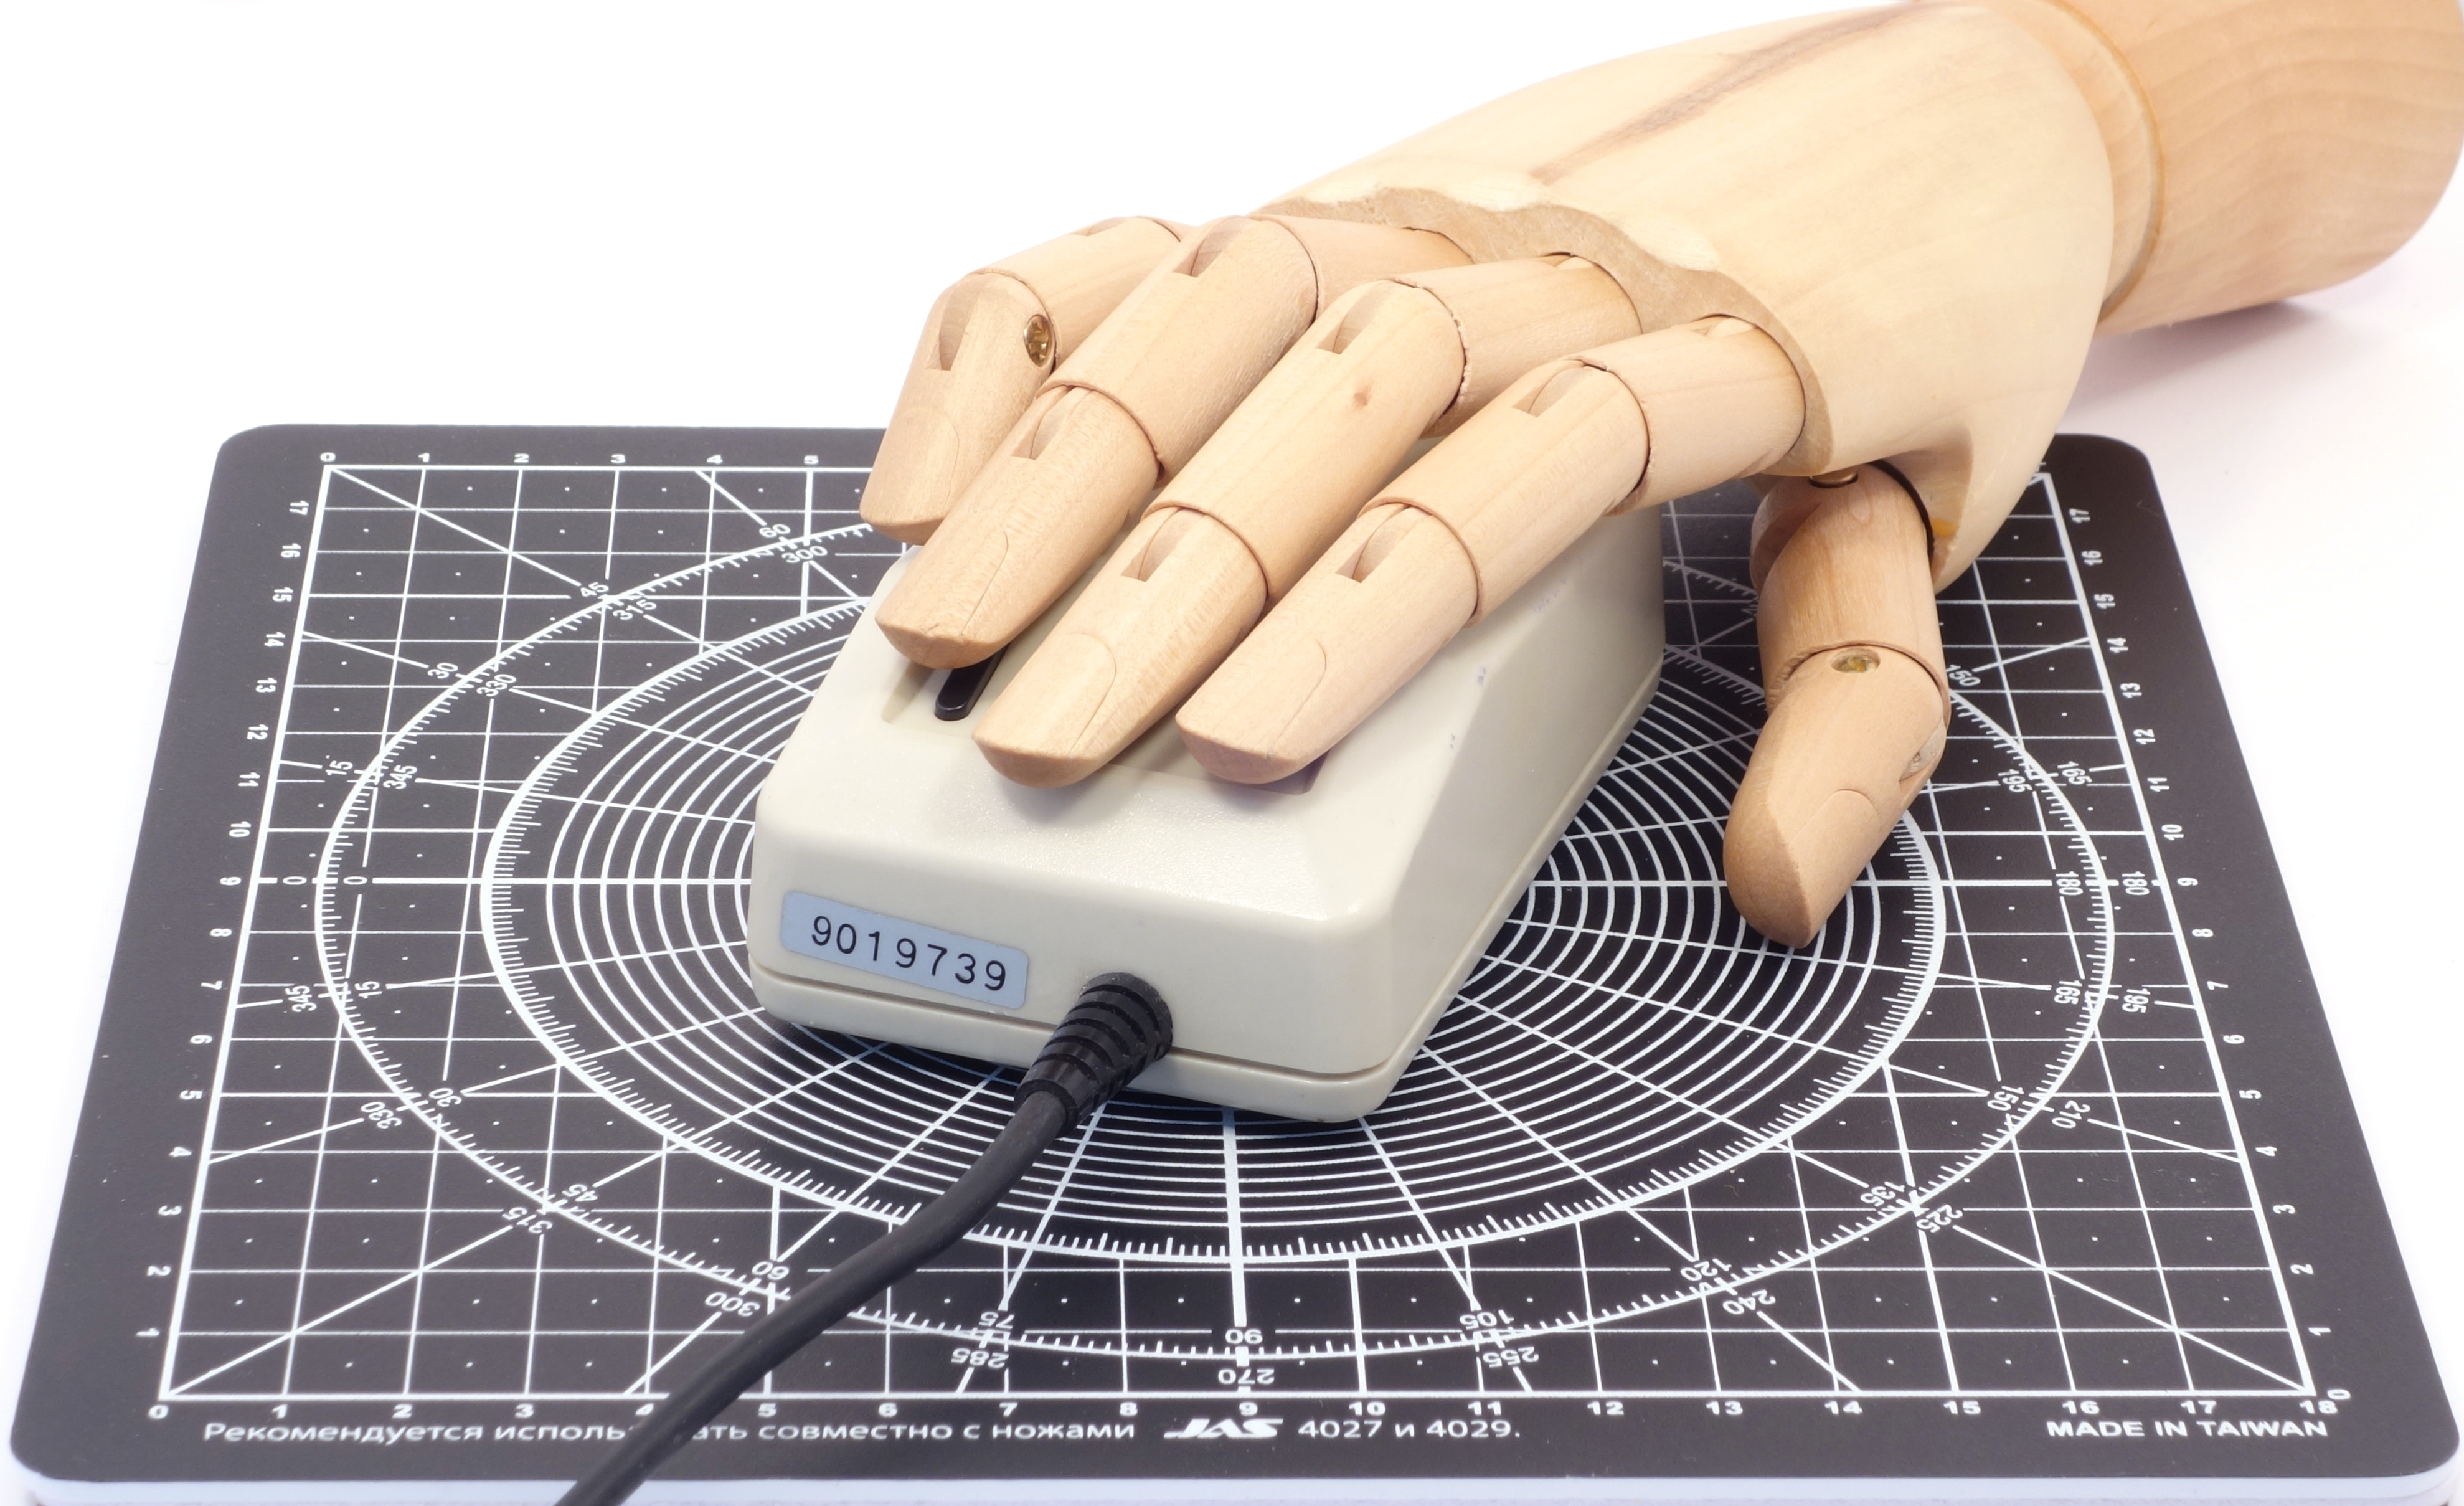
\includegraphics[scale=0.5]{1986_american_mouse/hand_30.jpg}
    \caption{American Mouse with a human hand model}
    \label{fig:AmericanHand}
\end{figure}

The Americanl Mouse has a D-SUB connector and an RS-232 interface. The device follows the Mouse Systems protocol, however this is not mentioned in the accompanying brochure. And when this mouse was on the market, the driver for this protocol could be found mainly bundled with Mouse Systems optical mice, which limited the possibility of using the American Mouse with third-party software. The only software package that came with the mouse was Compu-Brush, a rebranded PC Paint program.

\begin{figure}[h]
    \centering
    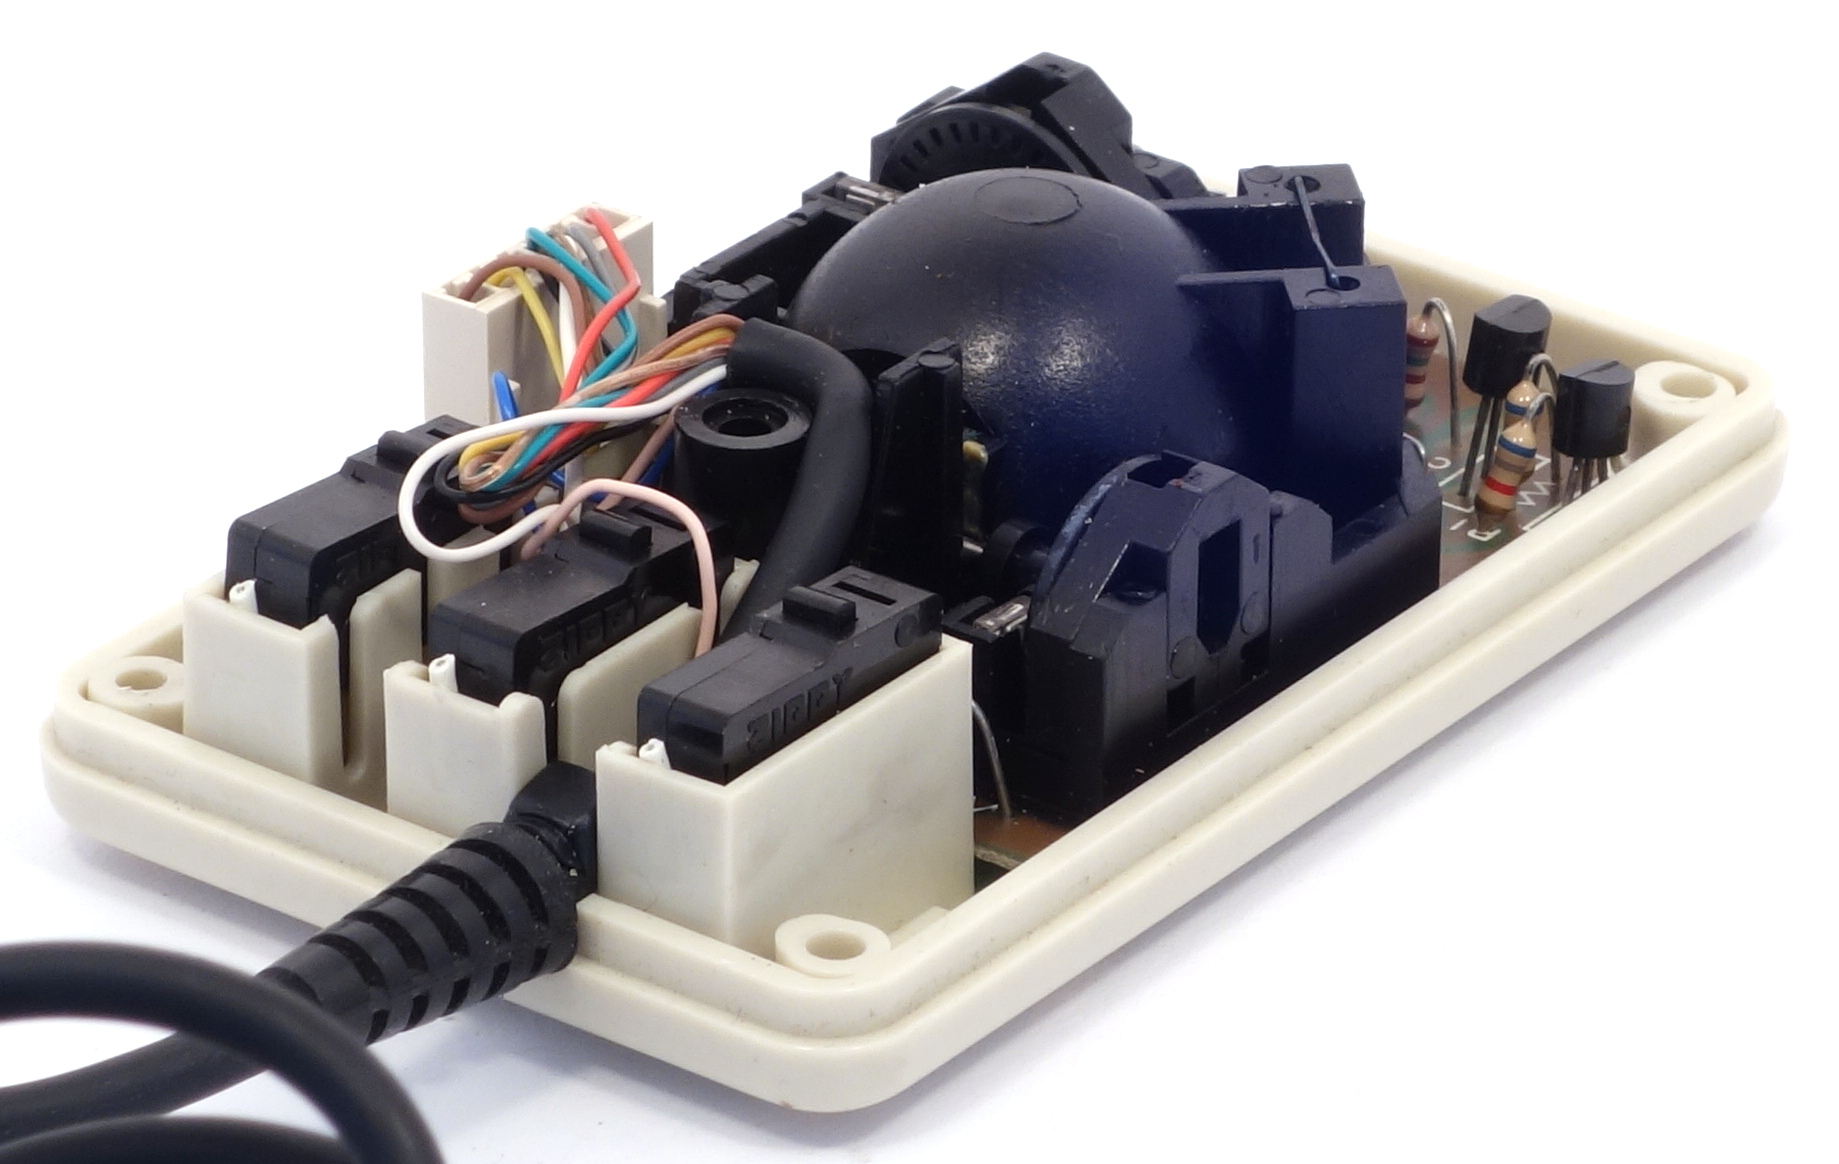
\includegraphics[scale=0.9]{1986_american_mouse/inside_60.jpg}
    \caption{American Mouse disassembled}
    \label{fig:AmericanInside}
\end{figure}

Trackball internals are shown on figure \ref{fig:AmericanInside}. The figure shows a fairly standard design of the opto-mechanical mouse. Worthy of mention is the dense filling of the internal space of the case with various plastic details that are absent in almost hollow optmechanical mice of a later period.

\begin{thebibliography}{9}
\bibitem {adv} I love American (advertising). // PC MAGAZINE, V. 5, No. 18. October 1986, p. 157. \url{https://archive.org/details/PC-Mag-1986-10-28/page/n159}
\bibitem {review} Barr Ch. Mice for mainstream applications // PC MAGAZINE, V. 6, No. 14., August 1987, pp. 119 – 146 \url{https://archive.org/details/PC-Mag-1987-08-01/page/n121}
\end{thebibliography}
\end{document}

\documentclass[11pt, a4paper]{article}
\usepackage{pdfpages}
\usepackage{parallel}
\usepackage[T2A]{fontenc}
\usepackage{ucs}
\usepackage[utf8x]{inputenc}
\usepackage[polish,english,russian]{babel}
\usepackage{hyperref}
\usepackage{rotating}
\usepackage[inner=2cm,top=1.8cm,outer=2cm,bottom=2.3cm,nohead]{geometry}
\usepackage{listings}
\usepackage{graphicx}
\usepackage{wrapfig}
\usepackage{longtable}
\usepackage{indentfirst}
\usepackage{array}
\usepackage{tikzsymbols}
\usepackage{soul}
\usepackage[ruled,vlined]{algorithm2e}
%\counterwithout{figure}{section} 

\usepackage{url}
\makeatletter
\g@addto@macro{\UrlBreaks}{\UrlOrds}
\makeatother

\newcolumntype{P}[1]{>{\raggedright\arraybackslash}p{#1}}
\frenchspacing
\usepackage{fixltx2e} %text sub- and superscripts
\usepackage{icomma} % коскі ў матэматычным рэжыме
\PreloadUnicodePage{4}

\newcommand{\longpage}{\enlargethispage{\baselineskip}}
\newcommand{\shortpage}{\enlargethispage{-\baselineskip}}

\def\switchlang#1{\expandafter\csname switchlang#1\endcsname}
\def\switchlangbe{
\let\saverefname=\refname%
\def\refname{Літаратура}%
\def\figurename{Іл.}%
}
\def\switchlangen{
\let\saverefname=\refname%
\def\refname{References}%
\def\figurename{Fig.}%
}
\def\switchlangru{
\let\saverefname=\refname%
\let\savefigurename=\figurename%
\def\refname{Литература}%
\def\figurename{Рис.}%
}

\hyphenation{admi-ni-stra-tive}
\hyphenation{ex-pe-ri-ence}
\hyphenation{fle-xi-bi-li-ty}
\hyphenation{Py-thon}
\hyphenation{ma-the-ma-ti-cal}
\hyphenation{re-ported}
\hyphenation{imp-le-menta-tions}
\hyphenation{pro-vides}
\hyphenation{en-gi-neering}
\hyphenation{com-pa-ti-bi-li-ty}
\hyphenation{im-pos-sible}
\hyphenation{desk-top}
\hyphenation{elec-tro-nic}
\hyphenation{com-pa-ny}
\hyphenation{de-ve-lop-ment}
\hyphenation{de-ve-loping}
\hyphenation{de-ve-lop}
\hyphenation{da-ta-ba-se}
\hyphenation{plat-forms}
\hyphenation{or-ga-ni-za-tion}
\hyphenation{pro-gramming}
\hyphenation{in-stru-ments}
\hyphenation{Li-nux}
\hyphenation{sour-ce}
\hyphenation{en-vi-ron-ment}
\hyphenation{Te-le-pathy}
\hyphenation{Li-nux-ov-ka}
\hyphenation{Open-BSD}
\hyphenation{Free-BSD}
\hyphenation{men-ti-on-ed}
\hyphenation{app-li-ca-tion}

\def\progref!#1!{\texttt{#1}}
\renewcommand{\arraystretch}{2} %Іначай формулы ў матрыцы зліпаюцца з лініямі
\usepackage{array}

\def\interview #1 (#2), #3, #4, #5\par{

\section[#1, #3, #4]{#1 -- #3, #4}
\def\qname{LVEE}
\def\aname{#1}
\def\q ##1\par{{\noindent \bf \qname: ##1 }\par}
\def\a{{\noindent \bf \aname: } \def\qname{L}\def\aname{#2}}
}

\def\interview* #1 (#2), #3, #4, #5\par{

\section*{#1\\{\small\rm #3, #4. #5}}
\ifx\ParallelWhichBox\undefined%
    \addcontentsline{toc}{section}{#1, #3, #4}%
\else%
\ifnum\ParallelWhichBox=0%
    \addcontentsline{toc}{section}{#1, #3, #4}%
\fi\fi%

\def\qname{LVEE}
\def\aname{#1}
\def\q ##1\par{{\noindent \bf \qname: ##1 }\par}
\def\a{{\noindent \bf \aname: } \def\qname{L}\def\aname{#2}}
}

\newcommand{\interviewfooter}[1]{
\vskip 1em
\noindent \textit{#1}
}

\switchlang{en}
\begin{document}

\title{1986 "--- NEC Crystal mouse}
\date{}
\maketitle
\selectlanguage{english}
In September 1986, NEC Corporation announced the EWS 4800 UNIX workstation. This computer was designed as a workstation for engineers to improve the efficiency of solving problems such as software development, computer-aided design, scientific and engineering calculations, and the collection and analysis of experimental data \cite{yt}. The computer was equipped with a graphical multi-window interface and a large 20-inch $1280 \times 1024 \times 256$ display. This powerful workstation came with the NEC Crystall Mouse (figure \ref{fig:NECCrystalPic}).

\begin{figure}[h]
    \centering
    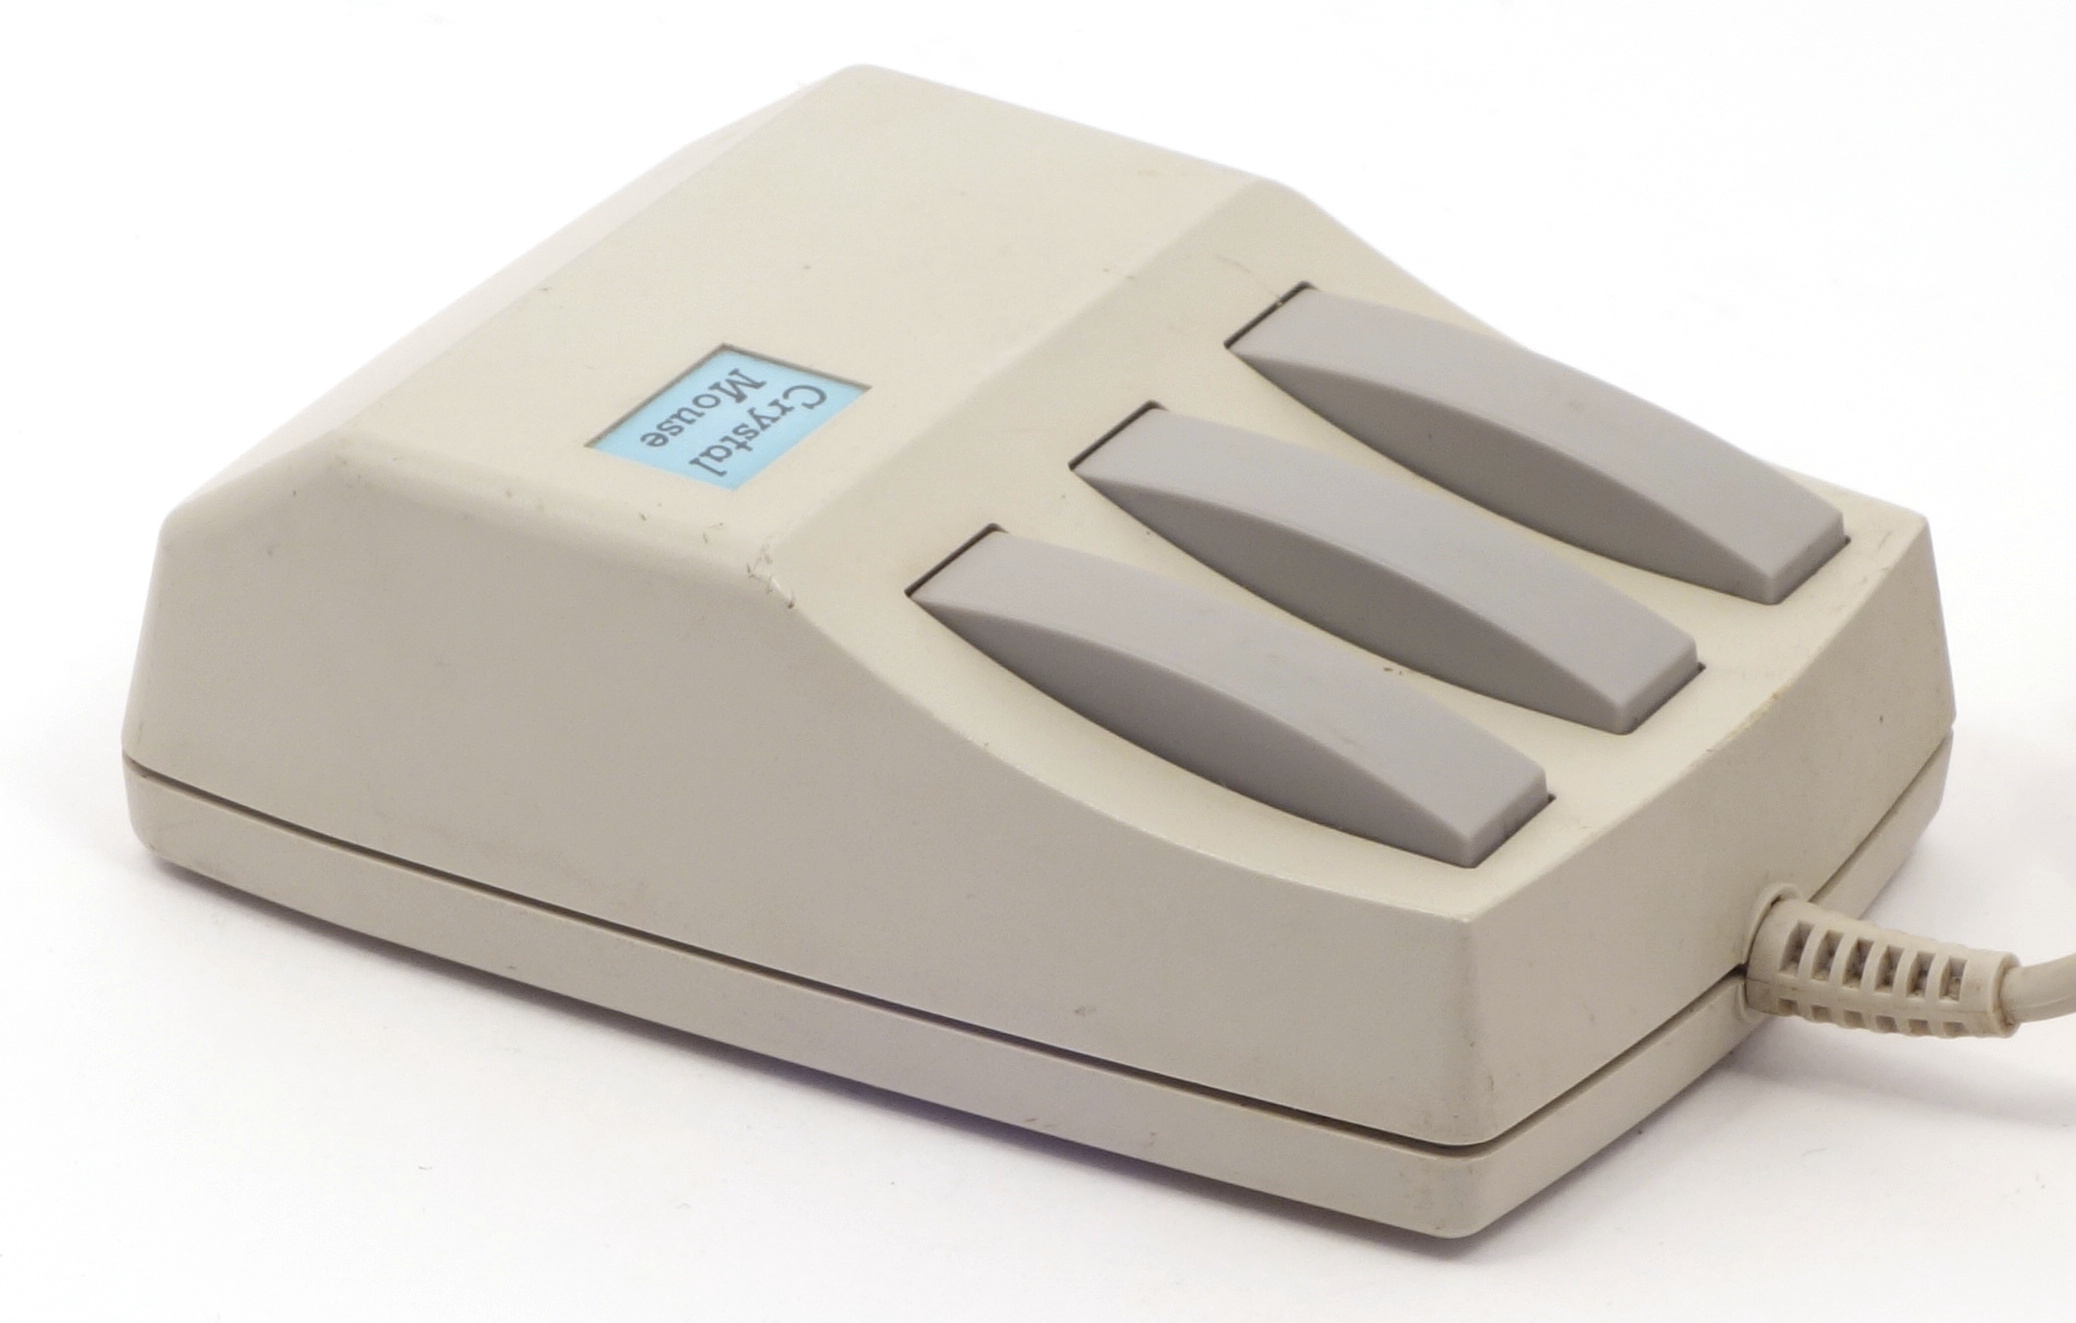
\includegraphics[scale=0.7]{1986_nec_crystal_mouse/necNorm_30.jpg}
    \caption{NEC Crystal Mouse}
    \label{fig:NECCrystalPic}
\end{figure}

The name of the mouse “Crystal Mouse” is highlighted on the upper side of the case with two triangular stylized mice in outlines and solid lines. The bottom side shows that this is an optical mouse (figure \ref{NecCrystalTopAndBottom}), which largely repeats the external design solutions of Mouse Systems mice of the same period and is intended for use with a special mirror pad \cite{photo}.

\begin{figure}[h]
    \centering
    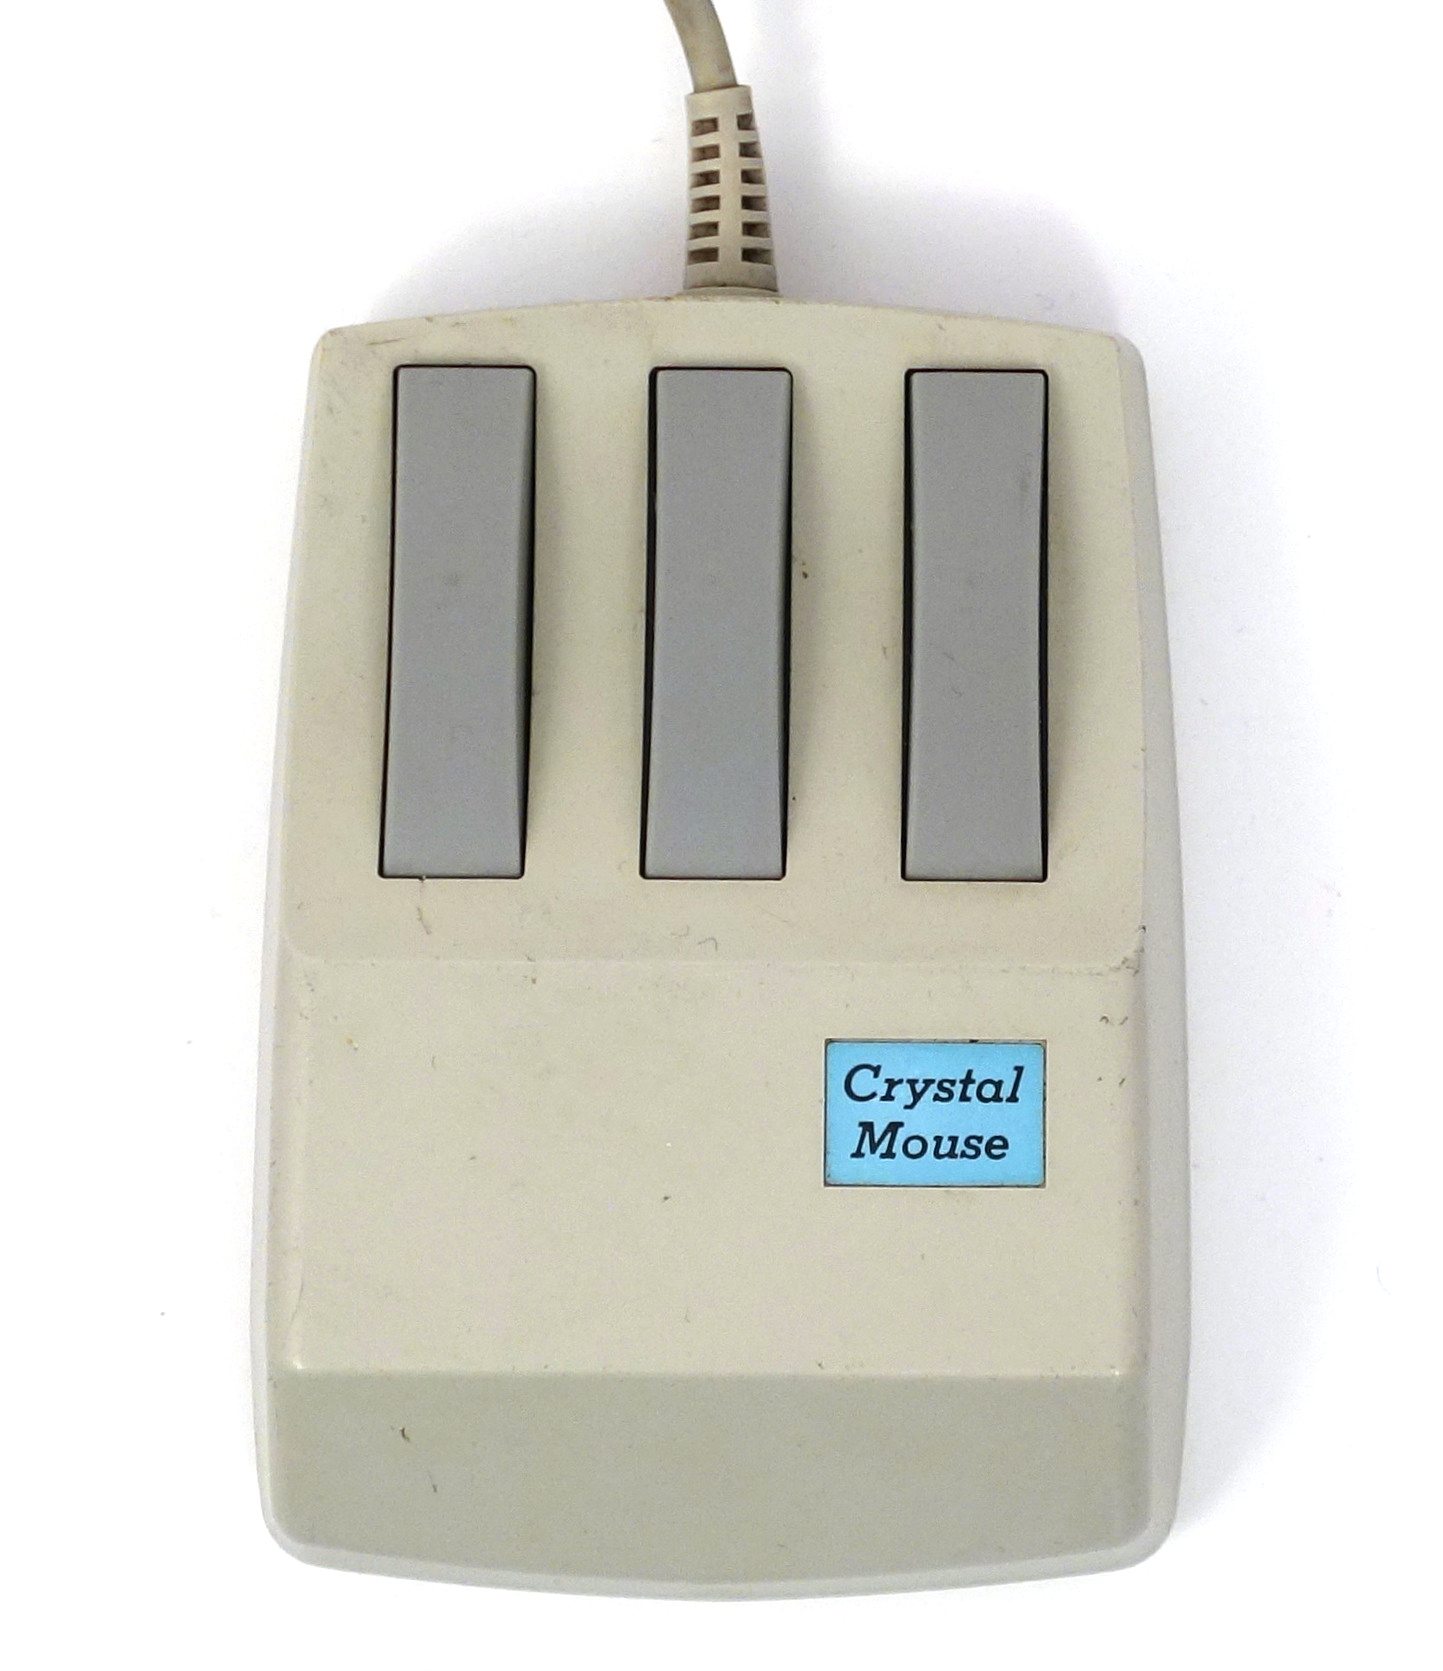
\includegraphics[scale=0.5]{1986_nec_crystal_mouse/nectop_60.jpg}
    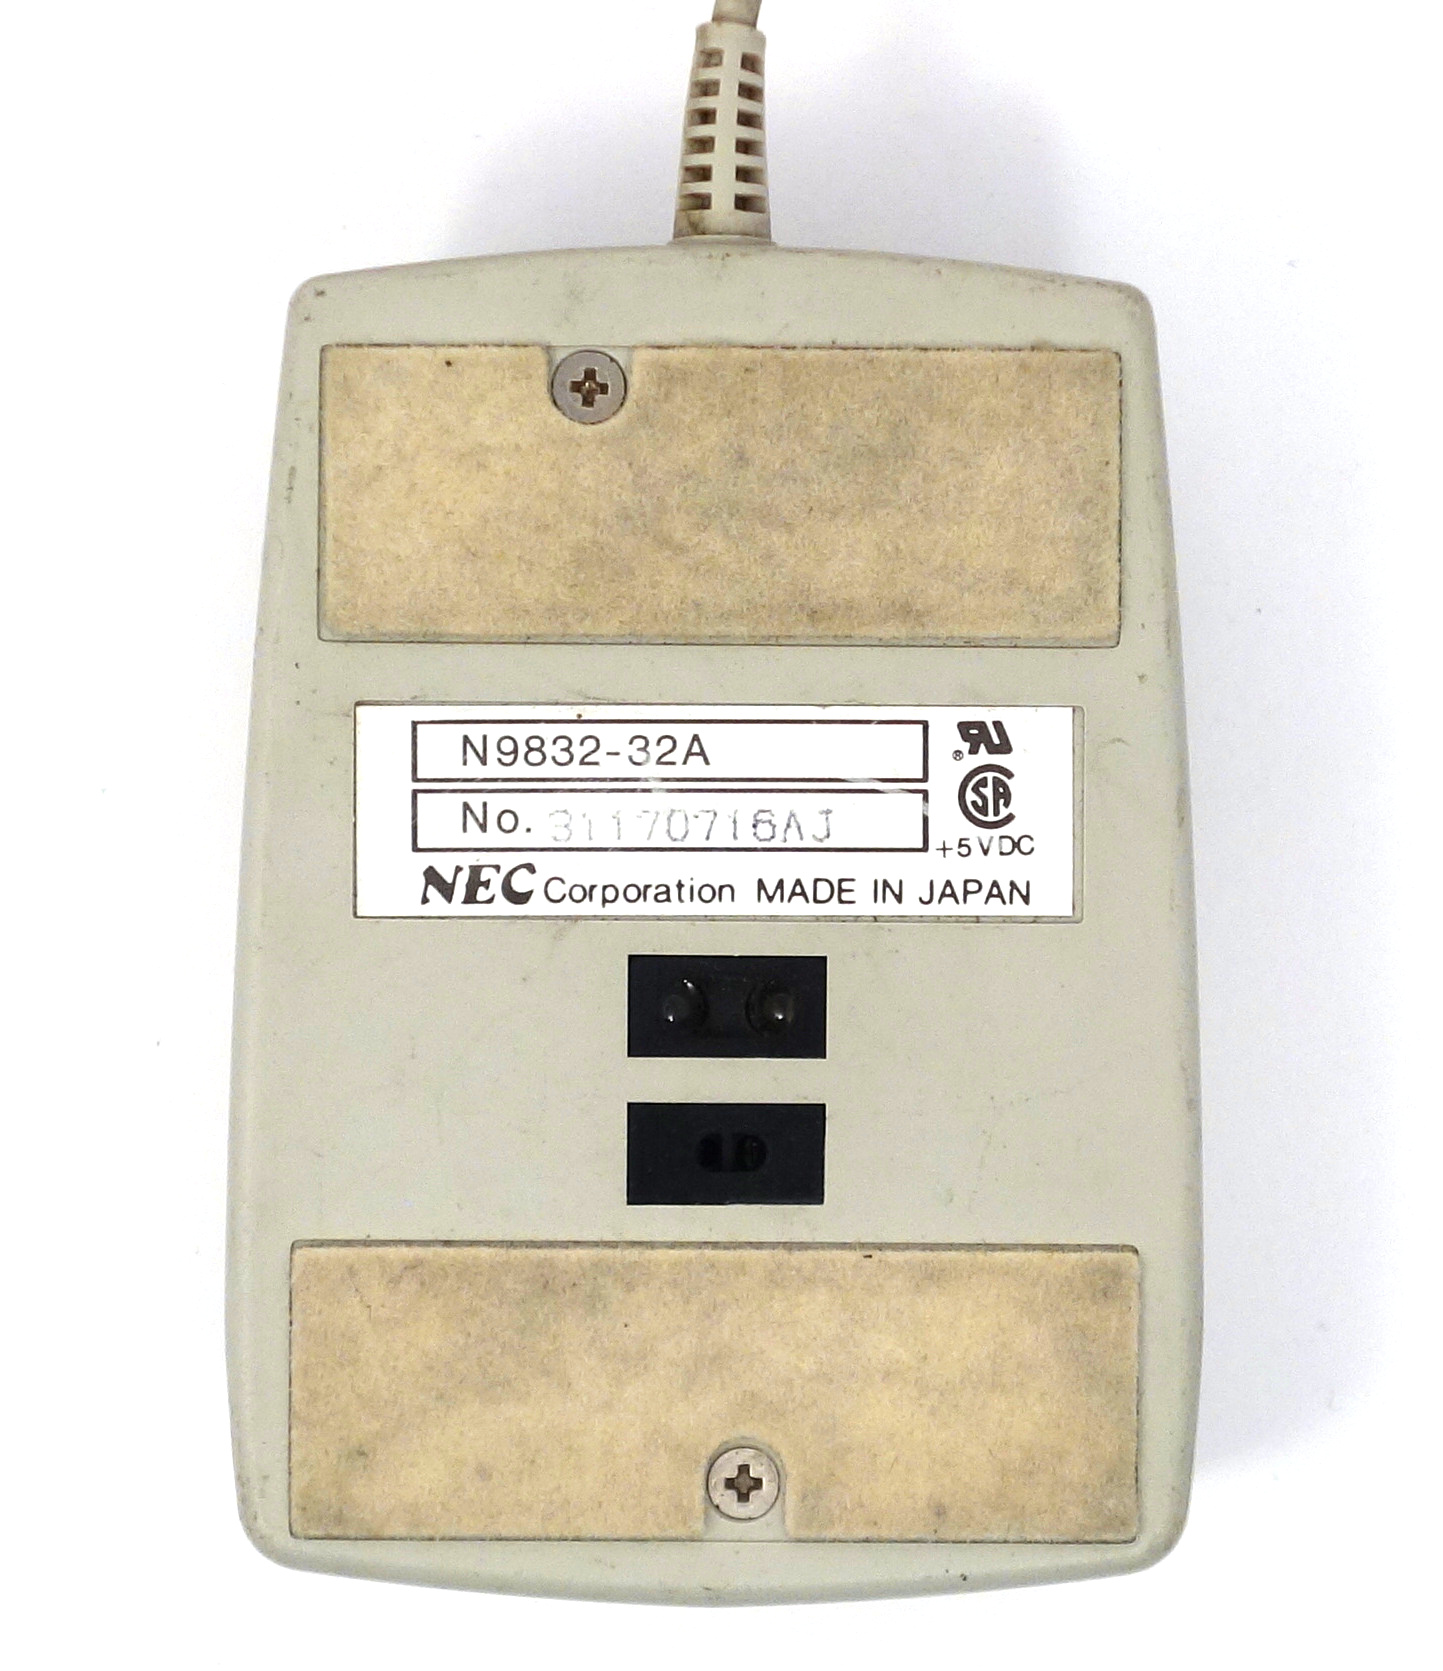
\includegraphics[scale=0.5]{1986_nec_crystal_mouse/necbottom_60.jpg}
    \caption{NEC Crystal Mouse, top and bottom views}
    \label{NecCrystalTopAndBottom}
\end{figure}

In terms of size, the manipulator is an optical cursor control device typical for the 80s (figure \ref{fig:NecCrystalSize}).

\begin{figure}[h]
    \centering
    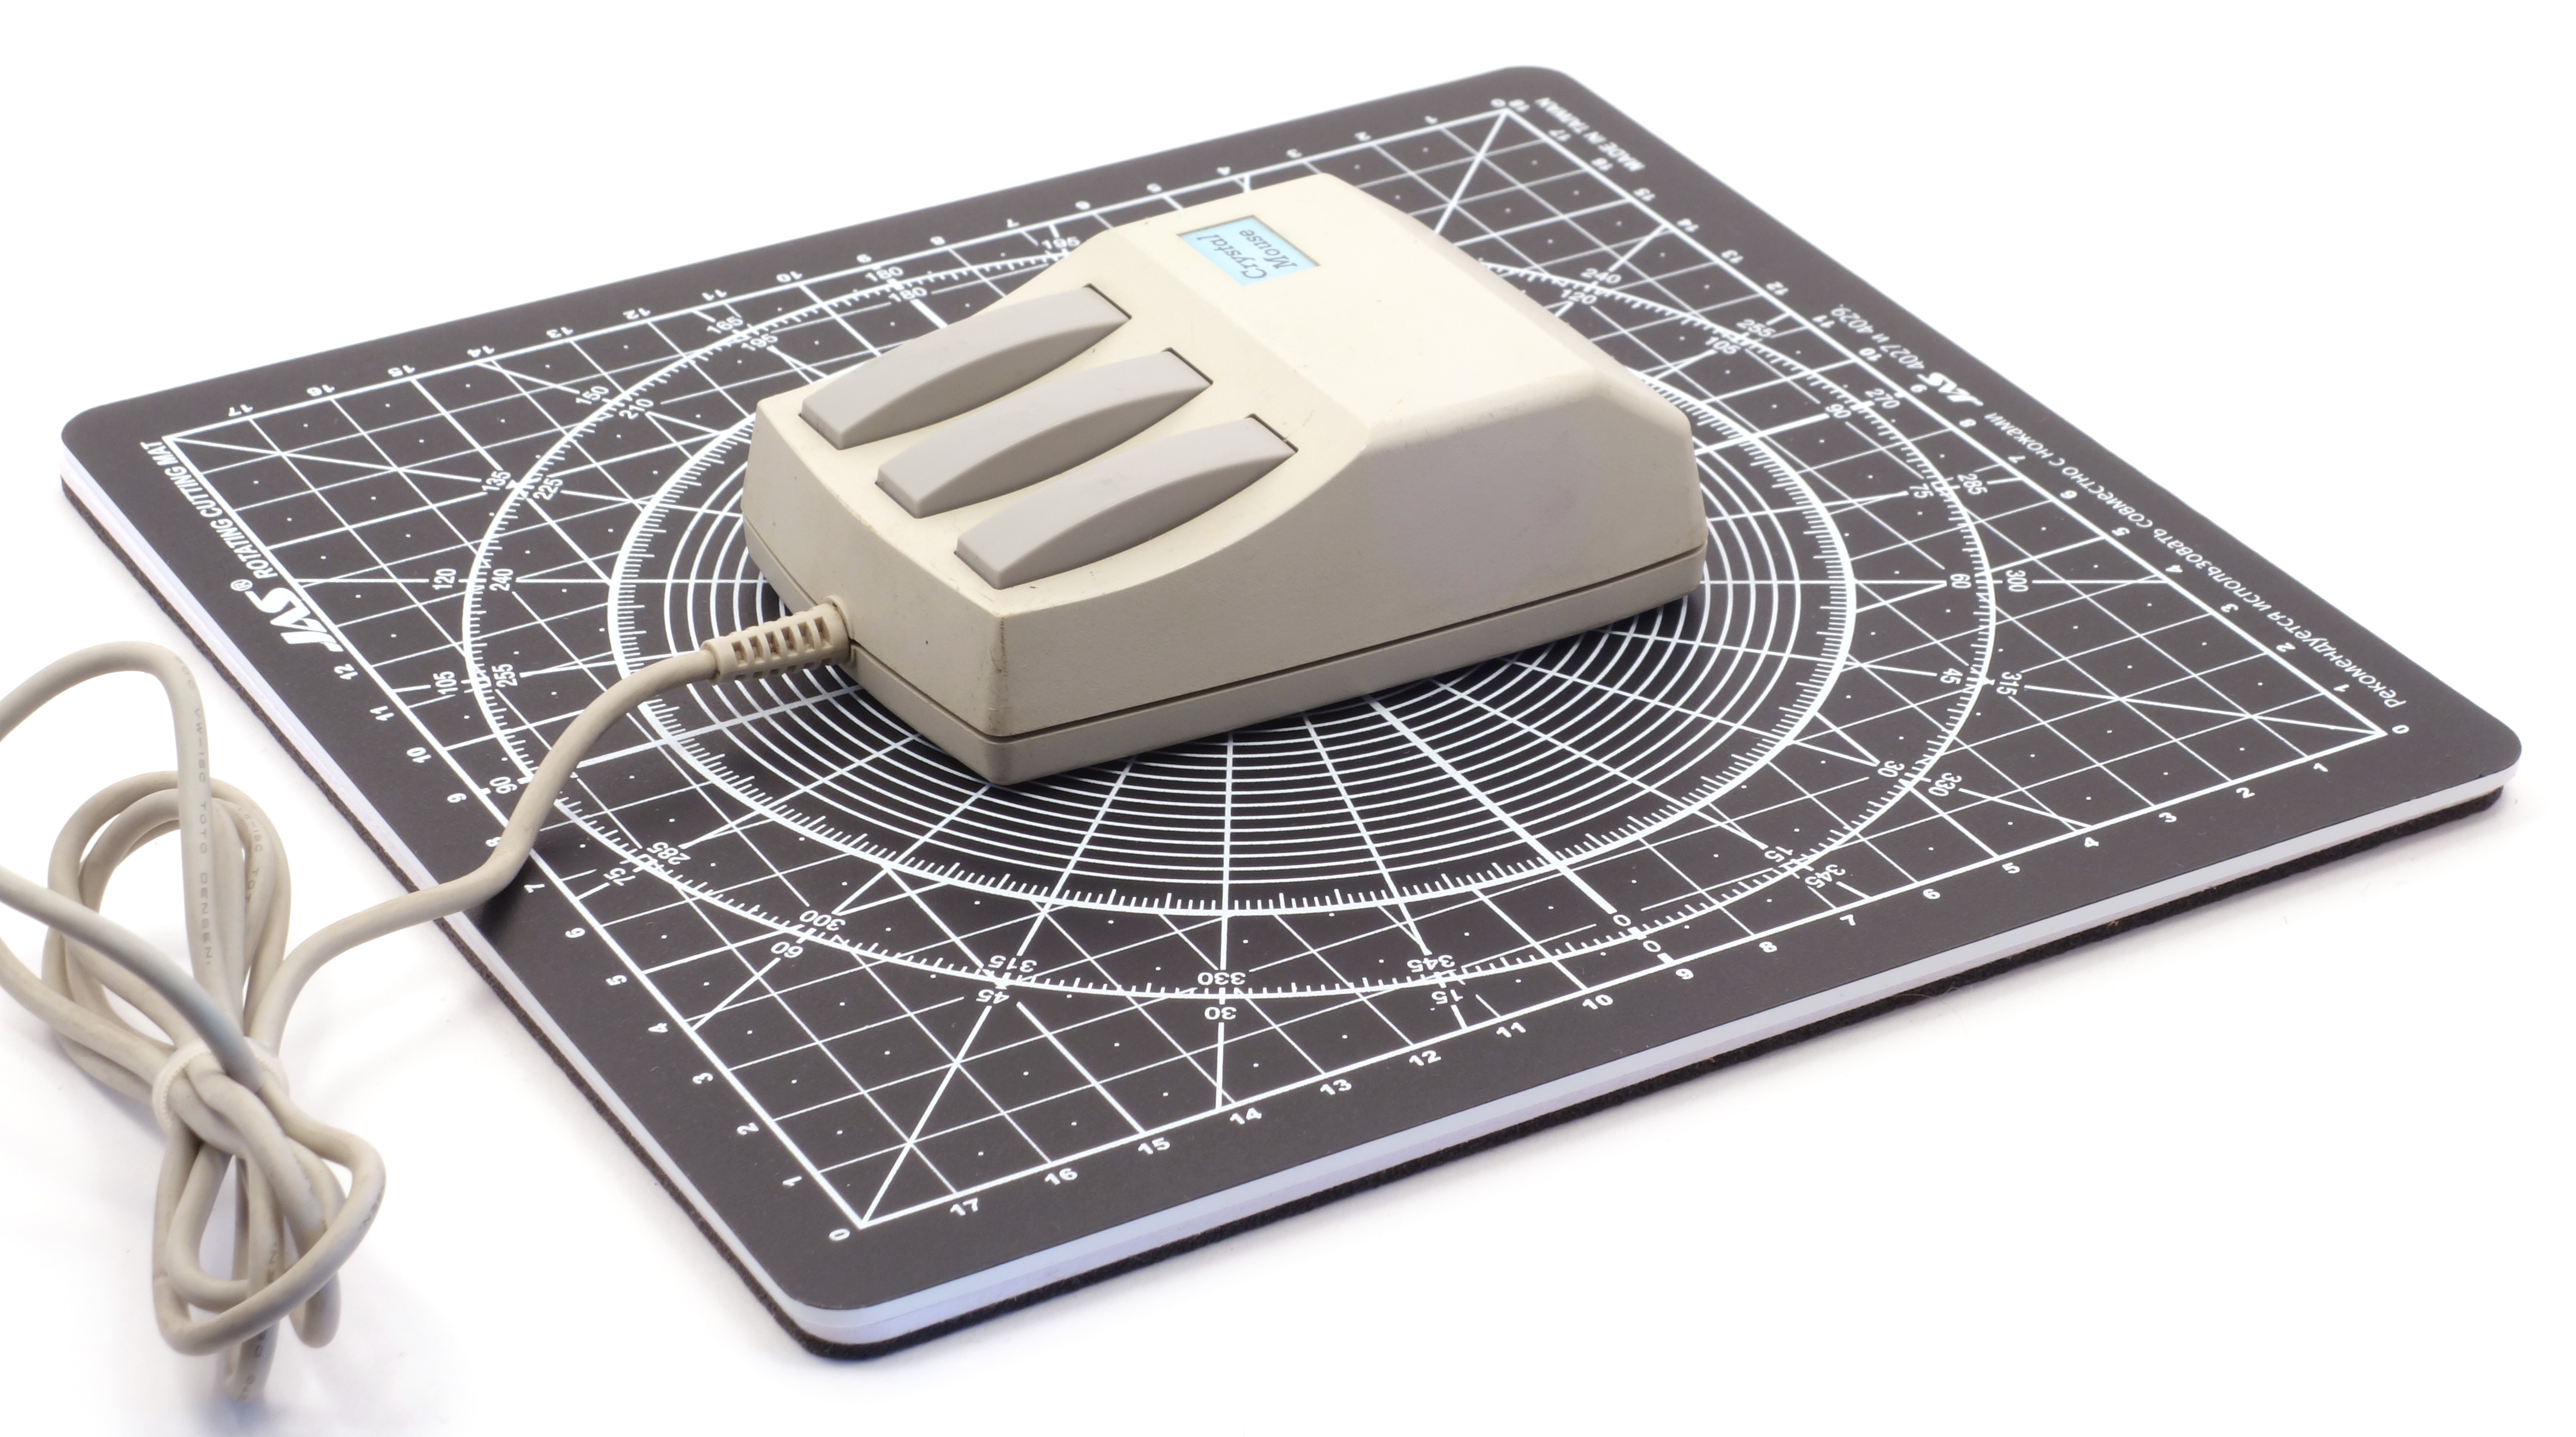
\includegraphics[scale=0.4]{1986_nec_crystal_mouse/NecKovrik_60.jpg}
    \caption{NEC Crystal Mouse on a graduated pad with a grid step of 1~cm}
    \label{fig:NecCrystalSize}
\end{figure}

In terms of ergonomics, the exterior of the Crystall Mouse has a strong industrial design. At the same time, a large number of corners and flat edges are partly compensated by rounded joints of the edges in the part of the body closest to the user and convex long buttons conveniently located within the reach of the fingers (figure \ref{fig:NecCrystalHand}).

\begin{figure}[h]
    \centering
    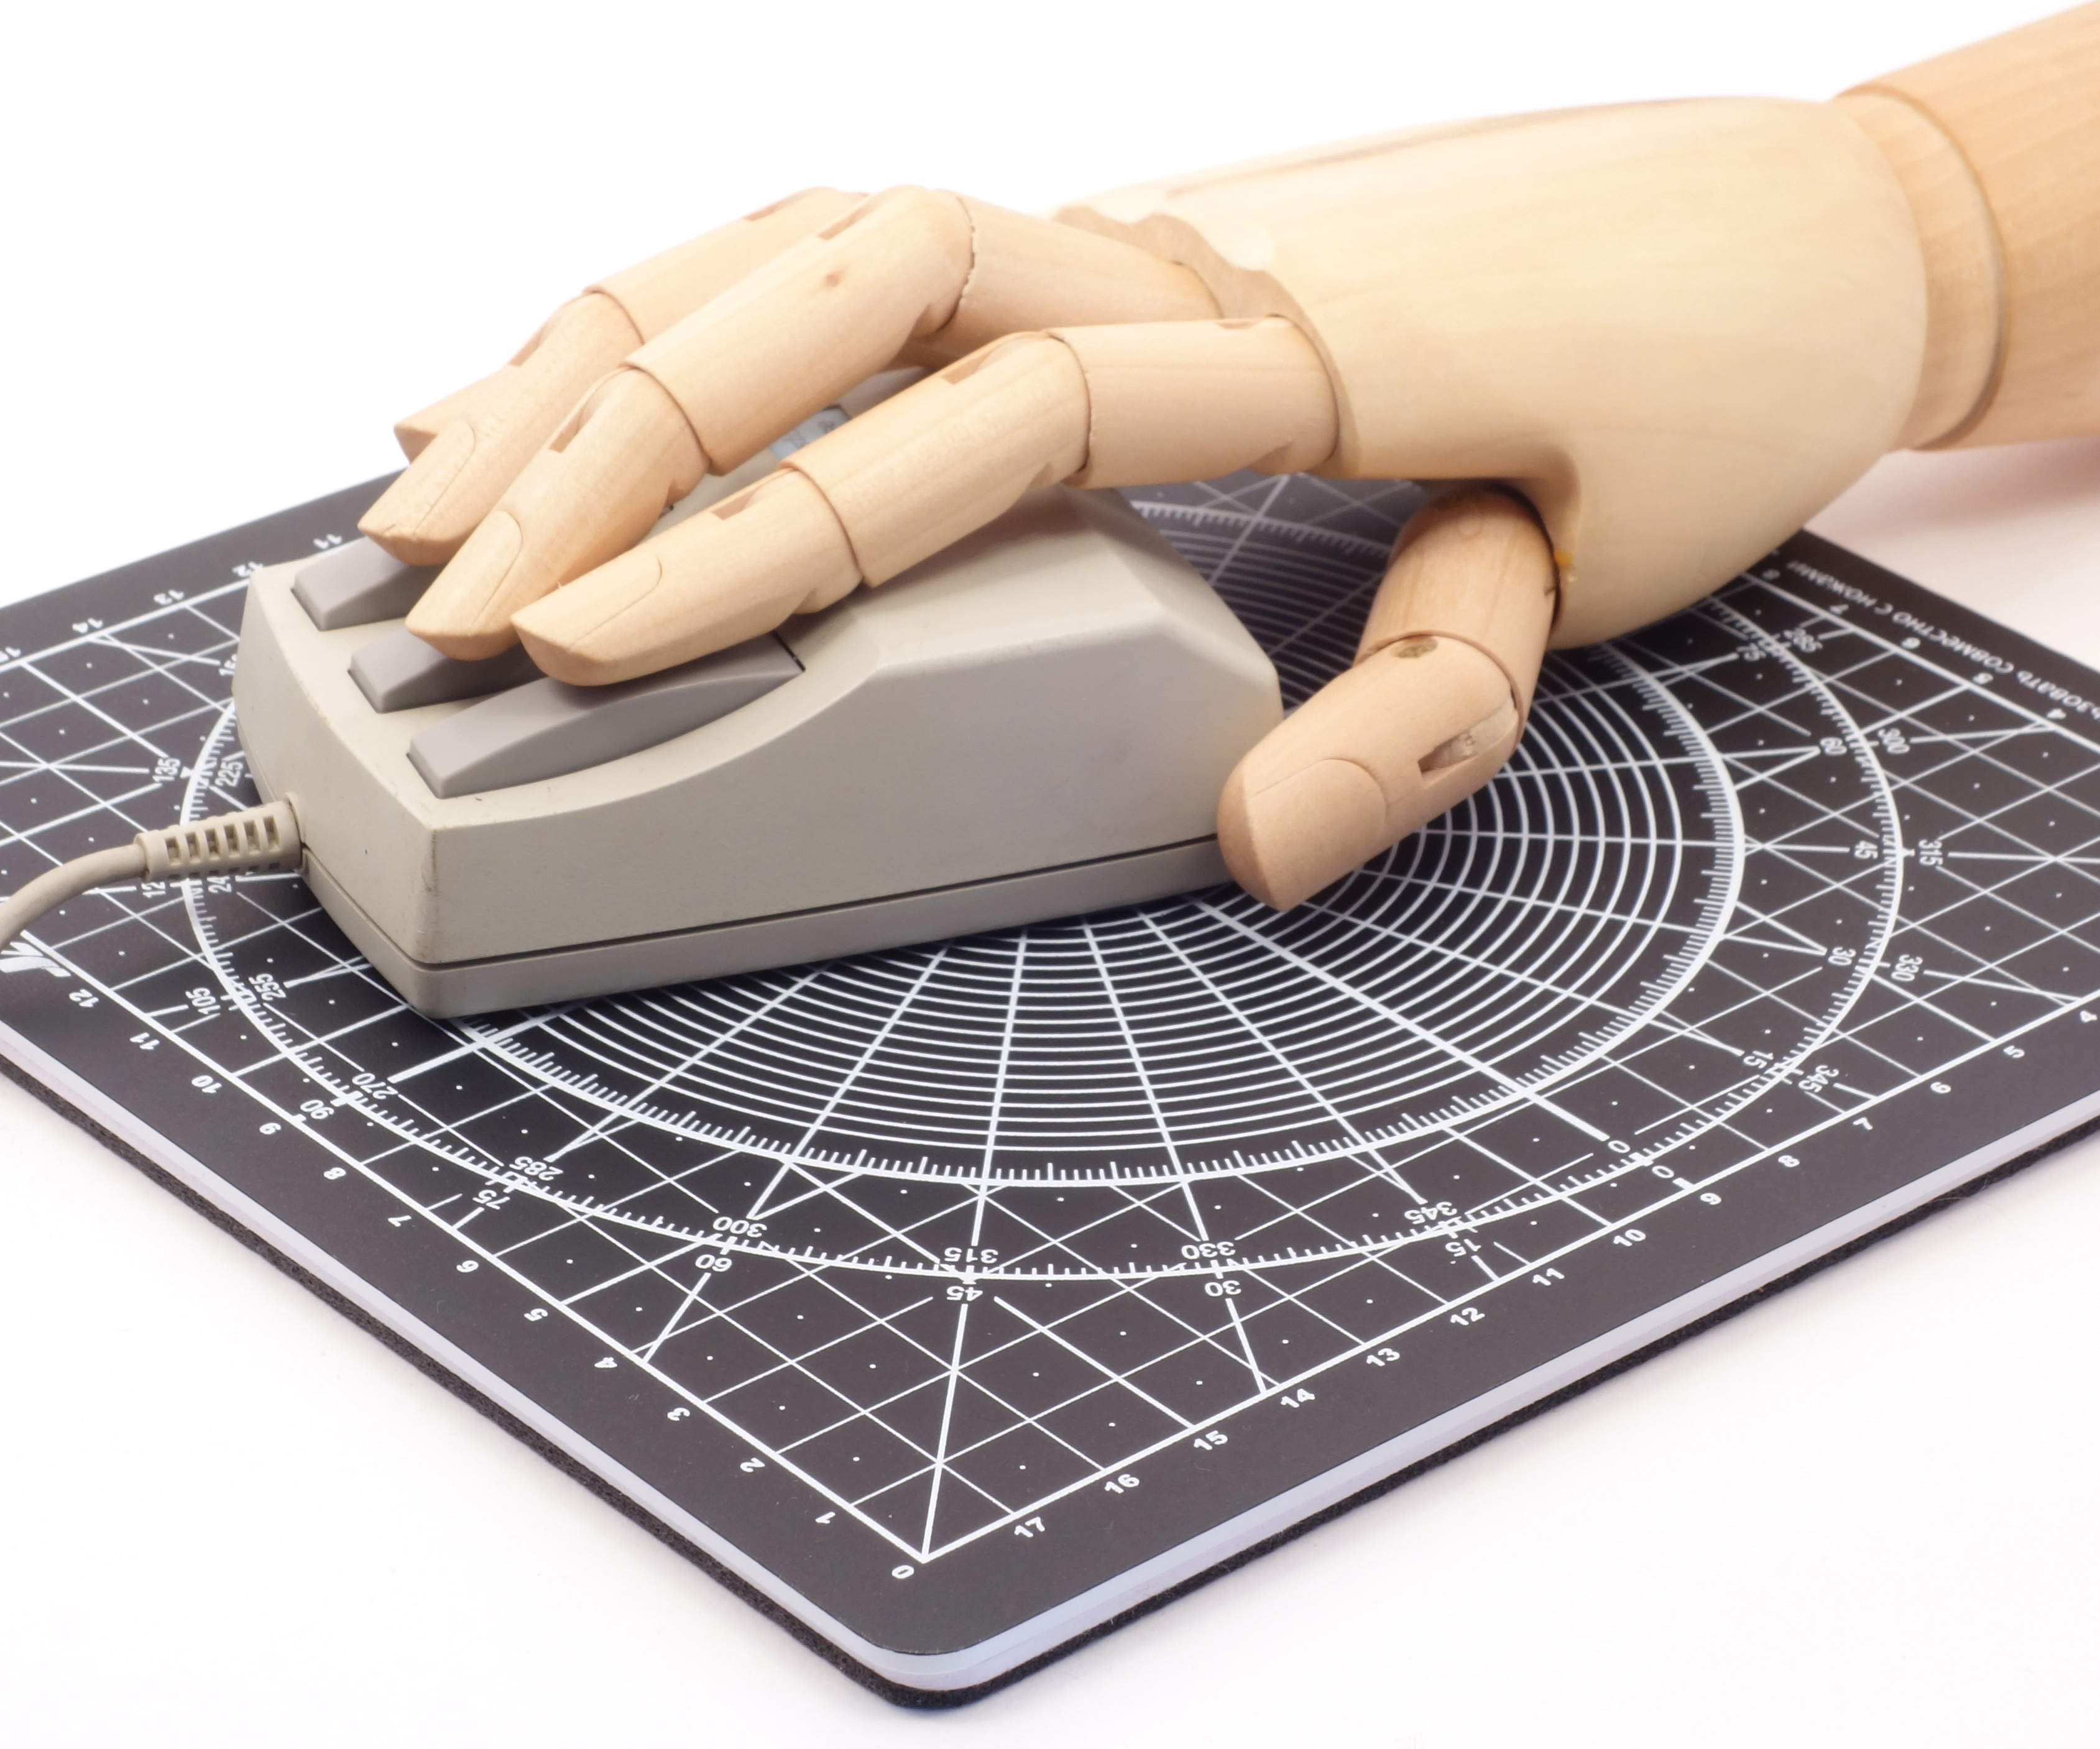
\includegraphics[scale=0.4]{1986_nec_crystal_mouse/NecRuka_30.jpg}
    \caption{NEC Crystal Mouse with a human hand model}
    \label{fig:NecCrystalHand}
\end{figure}

NEC Crystall Mouse has a DIN connector and belongs to the Bus Mouse category according to the connection interface. A feature of such mice is that the optocoupler signals are processed not by a chip in the mouse case, but by a special adapter in the computer system unit; therefore, this mouse is powered by the computer without a separate power supply, unlike many early optical models that were connected to the serial port of the IBM PC.

\begin{figure}[h]
    \centering
    \includegraphics[scale=0.8]{1986_nec_crystal_mouse/necraz_60.jpg}
    \caption{NEC Crystal Mouse disassembled}
    \label{fig:NecCrystalInside}
\end{figure}

Trackball internals are shown on figure \ref{fig:NecCrystalInside}. You can see the original design of this optical mouse. Unlike most optical mice of the 80s, it is not a direct copy of the Mouse Systems device, which has become a prototype for subsequent manipulators of this type.

\begin{thebibliography}{9}
\bibitem {yt} NEC EWS4800 \url{http://museum.ipsj.or.jp/en/computer/work/0003.html}
\bibitem {photo} Graphics NEC EWS4800 \url{http://www.cs.ce.nihon-u.ac.jp/facility/exp-gazo.html}
\end{thebibliography}
\end{document}

\documentclass[11pt, a4paper]{article}
\usepackage{pdfpages}
\usepackage{parallel}
\usepackage[T2A]{fontenc}
\usepackage{ucs}
\usepackage[utf8x]{inputenc}
\usepackage[polish,english,russian]{babel}
\usepackage{hyperref}
\usepackage{rotating}
\usepackage[inner=2cm,top=1.8cm,outer=2cm,bottom=2.3cm,nohead]{geometry}
\usepackage{listings}
\usepackage{graphicx}
\usepackage{wrapfig}
\usepackage{longtable}
\usepackage{indentfirst}
\usepackage{array}
\usepackage{tikzsymbols}
\usepackage{soul}
\usepackage[ruled,vlined]{algorithm2e}
%\counterwithout{figure}{section} 

\usepackage{url}
\makeatletter
\g@addto@macro{\UrlBreaks}{\UrlOrds}
\makeatother

\newcolumntype{P}[1]{>{\raggedright\arraybackslash}p{#1}}
\frenchspacing
\usepackage{fixltx2e} %text sub- and superscripts
\usepackage{icomma} % коскі ў матэматычным рэжыме
\PreloadUnicodePage{4}

\newcommand{\longpage}{\enlargethispage{\baselineskip}}
\newcommand{\shortpage}{\enlargethispage{-\baselineskip}}

\def\switchlang#1{\expandafter\csname switchlang#1\endcsname}
\def\switchlangbe{
\let\saverefname=\refname%
\def\refname{Літаратура}%
\def\figurename{Іл.}%
}
\def\switchlangen{
\let\saverefname=\refname%
\def\refname{References}%
\def\figurename{Fig.}%
}
\def\switchlangru{
\let\saverefname=\refname%
\let\savefigurename=\figurename%
\def\refname{Литература}%
\def\figurename{Рис.}%
}

\hyphenation{admi-ni-stra-tive}
\hyphenation{ex-pe-ri-ence}
\hyphenation{fle-xi-bi-li-ty}
\hyphenation{Py-thon}
\hyphenation{ma-the-ma-ti-cal}
\hyphenation{re-ported}
\hyphenation{imp-le-menta-tions}
\hyphenation{pro-vides}
\hyphenation{en-gi-neering}
\hyphenation{com-pa-ti-bi-li-ty}
\hyphenation{im-pos-sible}
\hyphenation{desk-top}
\hyphenation{elec-tro-nic}
\hyphenation{com-pa-ny}
\hyphenation{de-ve-lop-ment}
\hyphenation{de-ve-loping}
\hyphenation{de-ve-lop}
\hyphenation{da-ta-ba-se}
\hyphenation{plat-forms}
\hyphenation{or-ga-ni-za-tion}
\hyphenation{pro-gramming}
\hyphenation{in-stru-ments}
\hyphenation{Li-nux}
\hyphenation{sour-ce}
\hyphenation{en-vi-ron-ment}
\hyphenation{Te-le-pathy}
\hyphenation{Li-nux-ov-ka}
\hyphenation{Open-BSD}
\hyphenation{Free-BSD}
\hyphenation{men-ti-on-ed}
\hyphenation{app-li-ca-tion}

\def\progref!#1!{\texttt{#1}}
\renewcommand{\arraystretch}{2} %Іначай формулы ў матрыцы зліпаюцца з лініямі
\usepackage{array}

\def\interview #1 (#2), #3, #4, #5\par{

\section[#1, #3, #4]{#1 -- #3, #4}
\def\qname{LVEE}
\def\aname{#1}
\def\q ##1\par{{\noindent \bf \qname: ##1 }\par}
\def\a{{\noindent \bf \aname: } \def\qname{L}\def\aname{#2}}
}

\def\interview* #1 (#2), #3, #4, #5\par{

\section*{#1\\{\small\rm #3, #4. #5}}
\ifx\ParallelWhichBox\undefined%
    \addcontentsline{toc}{section}{#1, #3, #4}%
\else%
\ifnum\ParallelWhichBox=0%
    \addcontentsline{toc}{section}{#1, #3, #4}%
\fi\fi%

\def\qname{LVEE}
\def\aname{#1}
\def\q ##1\par{{\noindent \bf \qname: ##1 }\par}
\def\a{{\noindent \bf \aname: } \def\qname{L}\def\aname{#2}}
}

\newcommand{\interviewfooter}[1]{
\vskip 1em
\noindent \textit{#1}
}

\switchlang{en}
\begin{document}

\title{1986 "--- Honeywell microLYNX trackball}
\date{}
\maketitle
\selectlanguage{english}
The microLYNX trackball (or “$\mu LYNX$” if Greek characters are allowed) shown in figure \ref{fig:microLYNXPic} was manufactured in California by Honeywell, a subsidiary of Disc Instruments. Having appeared in 1986 or a year earlier (some of the advertising materials are dated 1985), the trackball proved to be a long-liver and subsequently withstood many incarnations as the model “LX200”, which differed in connection interfaces, electronics and were often rebranded under different company names \cite{lx200}.

\begin{figure}[h]
    \centering
    \includegraphics[scale=0.45]{1986_honeywell_microlynx_trackball/pic_30.jpg}
    \caption{Honeywell microLYNX trackball}
    \label{fig:microLYNXPic}
\end{figure}

As you can see, the device is made in a minimalist design, equipped with a large black ball recessed in a beige body with an extended wrist rest \ref{fig:microLYNXTopBottom}. The ball fits snugly to the edges of the hole in the device case, which protects well from debris getting inside the trackball, but makes it impossible to remove the ball for cleaning without disassembling the case. In front of the ball are three buttons with keycaps identical to the keys of the classic full-size keyboard of that time.

\begin{figure}[h]
    \centering
    \includegraphics[scale=0.4]{1986_honeywell_microlynx_trackball/top_30.jpg}
    \includegraphics[scale=0.4]{1986_honeywell_microlynx_trackball/bottom_30.jpg}
    \caption{microLYNX, top and bottom views}
    \label{fig:microLYNXTopBottom}
\end{figure}

Apparently, there were two early versions of the “LX200”: the comLYNX model had a serial \cite{comlynx} interface, the quadLYNX version was the most electronically simple quadrature device connected to the bus interface, while the most unusual of the three options, microLYNX, used the keyboard port as a connection interface, actually being included in the break of the keyboard cable. Later, variants with PS/2 interface also appeared.

By default, microLYNX operates in “text mode”, and turning the ball has the same effect as pressing the cursor keys on the keyboard: in fact, when the ball moves, the trackball generates and sends scan codes of the cursor keys to the computer. Trackball buttons are programmable: the user can configure the button to issue from 1 to 30 key codes in the form of macros. You can also adjust the cursor movement speed (how often the cursor key codes are generated).

The microLYNX driver can emulate a Microsoft mouse for graphics programs under DOS, and the user can use the trackball to move the cursor and do dragging to select text or move graphics (the two external buttons in front of the ball can be used to drag).

\begin{figure}[h]
    \centering
    \includegraphics[scale=0.4]{1986_honeywell_microlynx_trackball/size.jpg}
    \caption{microLYNX on a graduated pad with a grid step of 1~cm}
    \label{fig:microLYNXSize}
\end{figure}

However, given the size of the device (figure \ref{fig:microLYNXSize}), holding down the button while the ball is moving is a tricky maneuver at best. Honeywell solved this problem with the comLYNX trackball, which can use the middle button as a \cite{comlynx} drag latch. First, the middle button is pressed, then the left or right button, and this programmatically fixes the selected button in the pressed position. Repeated pressing of any of the three buttons disables this mode. However, microLYNX does not support this feature.

The trackball comes with two sets of software: a DOS driver that emulates a Microsoft mouse, and a separate DOS resident program that shows a pop-up menu and also allows you to program keyboard macros for the trackball buttons and cursor movement.

In addition, configuration can be performed without using a driver, in “alternative mode”, which is activated by pressing the “Ctrl + Alt + Shift” combination on the computer keyboard (due to the nature of the connection, microLYNX “listens” to everything that the keyboard sends to the computer). When entering this mode, the trackball prints text prompts to standard output (as if the user had just typed them) and asks the user to type special commands on the keyboard that change its settings.

\begin{figure}[h]
    \centering
    \includegraphics[scale=0.4]{1986_honeywell_microlynx_trackball/hand_60.jpg}
    \caption{microLYNX with a human hand model}
    \label{fig:microLYNXHand}
\end{figure}

In terms of ergonomics, the size of the trackball, the wrist rest, and the rounded edges and corners create a fairly comfortable working environment (figure \ref{fig:microLYNXHand}). However, the buttons are located far from the ball and significantly lower in height, which deprives the user of both the ability to press them with one hand without moving the hand, and with two hands, since the buttons are covered by the palm of the hand when the user rotates the ball. Therefore, microLYNX is difficult to use in a graphical interface that requires intensive work with both frequent cursor movements and button presses. However, the trackball can be quite effective in various industrial applications.

\begin{figure}[h]
    \centering
    \includegraphics[scale=0.52]{1986_honeywell_microlynx_trackball/inside_60.jpg}
    \caption{microLYNX disassembled}
    \label{fig:microLYNXInside}
\end{figure}

Trackball internals are shown on figure \ref{fig:microLYNXInside}. This is an optomechanical device. Rollers are made using bearings and stainless steel shafts, which ensures maximum reliability and durability of the device. The high reliability of trackball and ergonomics, which is well suitable for a number of technical tasks, made this model “long-term survivor”: the device has been produced for at least ten years for industrial applications under various brands, and at the same time a constant appearance and mechanical part of the structure were preserved.

\begin{thebibliography}{9}
\bibitem {comlynx} Trackballs: Stationary mice // PC Magazine. August 1987, page 199-202 \url{https://trackballs.eu/media/Fulcrum/PC%20Mag%20Aug-1987%20p199-202.pdf}
\bibitem {lx200} Disc Instruments LX200 \url{https://web.archive.org/web/20220501213039/https://forum.trackballs.eu/viewtopic.php?f=17&t=16}
\end{thebibliography}
\end{document}

\documentclass[11pt, a4paper]{article}
\usepackage{pdfpages}
\usepackage{parallel}
\usepackage[T2A]{fontenc}
\usepackage{ucs}
\usepackage[utf8x]{inputenc}
\usepackage[polish,english,russian]{babel}
\usepackage{hyperref}
\usepackage{rotating}
\usepackage[inner=2cm,top=1.8cm,outer=2cm,bottom=2.3cm,nohead]{geometry}
\usepackage{listings}
\usepackage{graphicx}
\usepackage{wrapfig}
\usepackage{longtable}
\usepackage{indentfirst}
\usepackage{array}
\usepackage{tikzsymbols}
\usepackage{soul}
\usepackage[ruled,vlined]{algorithm2e}
%\counterwithout{figure}{section} 

\usepackage{url}
\makeatletter
\g@addto@macro{\UrlBreaks}{\UrlOrds}
\makeatother

\newcolumntype{P}[1]{>{\raggedright\arraybackslash}p{#1}}
\frenchspacing
\usepackage{fixltx2e} %text sub- and superscripts
\usepackage{icomma} % коскі ў матэматычным рэжыме
\PreloadUnicodePage{4}

\newcommand{\longpage}{\enlargethispage{\baselineskip}}
\newcommand{\shortpage}{\enlargethispage{-\baselineskip}}

\def\switchlang#1{\expandafter\csname switchlang#1\endcsname}
\def\switchlangbe{
\let\saverefname=\refname%
\def\refname{Літаратура}%
\def\figurename{Іл.}%
}
\def\switchlangen{
\let\saverefname=\refname%
\def\refname{References}%
\def\figurename{Fig.}%
}
\def\switchlangru{
\let\saverefname=\refname%
\let\savefigurename=\figurename%
\def\refname{Литература}%
\def\figurename{Рис.}%
}

\hyphenation{admi-ni-stra-tive}
\hyphenation{ex-pe-ri-ence}
\hyphenation{fle-xi-bi-li-ty}
\hyphenation{Py-thon}
\hyphenation{ma-the-ma-ti-cal}
\hyphenation{re-ported}
\hyphenation{imp-le-menta-tions}
\hyphenation{pro-vides}
\hyphenation{en-gi-neering}
\hyphenation{com-pa-ti-bi-li-ty}
\hyphenation{im-pos-sible}
\hyphenation{desk-top}
\hyphenation{elec-tro-nic}
\hyphenation{com-pa-ny}
\hyphenation{de-ve-lop-ment}
\hyphenation{de-ve-loping}
\hyphenation{de-ve-lop}
\hyphenation{da-ta-ba-se}
\hyphenation{plat-forms}
\hyphenation{or-ga-ni-za-tion}
\hyphenation{pro-gramming}
\hyphenation{in-stru-ments}
\hyphenation{Li-nux}
\hyphenation{sour-ce}
\hyphenation{en-vi-ron-ment}
\hyphenation{Te-le-pathy}
\hyphenation{Li-nux-ov-ka}
\hyphenation{Open-BSD}
\hyphenation{Free-BSD}
\hyphenation{men-ti-on-ed}
\hyphenation{app-li-ca-tion}

\def\progref!#1!{\texttt{#1}}
\renewcommand{\arraystretch}{2} %Іначай формулы ў матрыцы зліпаюцца з лініямі
\usepackage{array}

\def\interview #1 (#2), #3, #4, #5\par{

\section[#1, #3, #4]{#1 -- #3, #4}
\def\qname{LVEE}
\def\aname{#1}
\def\q ##1\par{{\noindent \bf \qname: ##1 }\par}
\def\a{{\noindent \bf \aname: } \def\qname{L}\def\aname{#2}}
}

\def\interview* #1 (#2), #3, #4, #5\par{

\section*{#1\\{\small\rm #3, #4. #5}}
\ifx\ParallelWhichBox\undefined%
    \addcontentsline{toc}{section}{#1, #3, #4}%
\else%
\ifnum\ParallelWhichBox=0%
    \addcontentsline{toc}{section}{#1, #3, #4}%
\fi\fi%

\def\qname{LVEE}
\def\aname{#1}
\def\q ##1\par{{\noindent \bf \qname: ##1 }\par}
\def\a{{\noindent \bf \aname: } \def\qname{L}\def\aname{#2}}
}

\newcommand{\interviewfooter}[1]{
\vskip 1em
\noindent \textit{#1}
}


\begin{document}

\title{1987 "--- IBM PS/2 mouse}
\date{}
\maketitle

This mouse, released in 1987, was the first to implement the PS/2 interface, which is still used in a number of desktop computers to connect keyboards and mice using a 6-pin mini-DIN connector.

\begin{figure}[h]
    \centering
    \includegraphics[width=\textwidth]{1987_ibm_ps2_mouse/num0.JPG}
    \caption{IBM PS/2 Mouse}
    \label{fig:IMBPS2Pic}
\end{figure}

The first mouse with this interface was this device from IBM, available at relatively consumer prices in the late 80s. As you can see (figure \ref{fig:IMBPS2TopBottom}), there are two mechanical buttons and an embossed company logo on the top side of the case; in general, the case is minimalistic and, apart from that, does not contain any additional elements. The bottom contains the ball, and the two arrows on the ball's locking ring show the direction to unlock so it can be removed for cleaning the mouse.

\begin{figure}[h]
    \centering
    \includegraphics[scale=0.6]{1987_ibm_ps2_mouse/num1.JPG}
    \includegraphics[scale=0.6]{1987_ibm_ps2_mouse/num2.JPG}
    \caption{IBM PS/2 Mouse, top and bottom views}
    \label{fig:IMBPS2TopBottom}
\end{figure}

\begin{figure}[h]
    \centering
    \includegraphics[scale=0.4]{1987_ibm_ps2_mouse/num3.JPG}
    \caption{IBM PS/2 Mouse with a human hand model}
    \label{fig:IMBPS2Hand}
\end{figure}

As you can see in figure \ref{fig:IMBPS2Hand}, the trapezoidal shape of the case allows you to wrap your fingers comfortably around the mouse and press the buttons in the natural position of the hand; however, the small size of the mouse (figure \ref{fig:IMBPS2Size}) does not allow the palm of the hand to rest on the body of the mouse, which puts additional strain on the wrist.

\begin{figure}[h]
    \centering
    \includegraphics[scale=0.34]{1987_ibm_ps2_mouse/num4.jpg}
    \caption{Изображение IBM PS/2 Mouse on a graduated pad with a grid step of 1~cm}
    \label{fig:IBMPS2Size}
\end{figure}

\begin{figure}[h]
    \centering
    \includegraphics[scale=0.7]{1987_ibm_ps2_mouse/razob1.jpg} 
    \caption{IBM PS/2 Mouse disassembled}
    \label{fig:IBMPS2Inside}
\end{figure}

IBM PS/2 Mouse internals are shown on figure \ref{fig:IBMPS2Inside}. The mouse is a device with a contact encoder made in Japan by Alps. Also, massive metal rollers with bearings should be noted, since they are typical for expensive manipulators.

\end{document}

\documentclass[11pt, a4paper]{article}
\usepackage{pdfpages}
\usepackage{parallel}
\usepackage[T2A]{fontenc}
\usepackage{ucs}
\usepackage[utf8x]{inputenc}
\usepackage[polish,english,russian]{babel}
\usepackage{hyperref}
\usepackage{rotating}
\usepackage[inner=2cm,top=1.8cm,outer=2cm,bottom=2.3cm,nohead]{geometry}
\usepackage{listings}
\usepackage{graphicx}
\usepackage{wrapfig}
\usepackage{longtable}
\usepackage{indentfirst}
\usepackage{array}
\usepackage{tikzsymbols}
\usepackage{soul}
\usepackage[ruled,vlined]{algorithm2e}
%\counterwithout{figure}{section} 

\usepackage{url}
\makeatletter
\g@addto@macro{\UrlBreaks}{\UrlOrds}
\makeatother

\newcolumntype{P}[1]{>{\raggedright\arraybackslash}p{#1}}
\frenchspacing
\usepackage{fixltx2e} %text sub- and superscripts
\usepackage{icomma} % коскі ў матэматычным рэжыме
\PreloadUnicodePage{4}

\newcommand{\longpage}{\enlargethispage{\baselineskip}}
\newcommand{\shortpage}{\enlargethispage{-\baselineskip}}

\def\switchlang#1{\expandafter\csname switchlang#1\endcsname}
\def\switchlangbe{
\let\saverefname=\refname%
\def\refname{Літаратура}%
\def\figurename{Іл.}%
}
\def\switchlangen{
\let\saverefname=\refname%
\def\refname{References}%
\def\figurename{Fig.}%
}
\def\switchlangru{
\let\saverefname=\refname%
\let\savefigurename=\figurename%
\def\refname{Литература}%
\def\figurename{Рис.}%
}

\hyphenation{admi-ni-stra-tive}
\hyphenation{ex-pe-ri-ence}
\hyphenation{fle-xi-bi-li-ty}
\hyphenation{Py-thon}
\hyphenation{ma-the-ma-ti-cal}
\hyphenation{re-ported}
\hyphenation{imp-le-menta-tions}
\hyphenation{pro-vides}
\hyphenation{en-gi-neering}
\hyphenation{com-pa-ti-bi-li-ty}
\hyphenation{im-pos-sible}
\hyphenation{desk-top}
\hyphenation{elec-tro-nic}
\hyphenation{com-pa-ny}
\hyphenation{de-ve-lop-ment}
\hyphenation{de-ve-loping}
\hyphenation{de-ve-lop}
\hyphenation{da-ta-ba-se}
\hyphenation{plat-forms}
\hyphenation{or-ga-ni-za-tion}
\hyphenation{pro-gramming}
\hyphenation{in-stru-ments}
\hyphenation{Li-nux}
\hyphenation{sour-ce}
\hyphenation{en-vi-ron-ment}
\hyphenation{Te-le-pathy}
\hyphenation{Li-nux-ov-ka}
\hyphenation{Open-BSD}
\hyphenation{Free-BSD}
\hyphenation{men-ti-on-ed}
\hyphenation{app-li-ca-tion}

\def\progref!#1!{\texttt{#1}}
\renewcommand{\arraystretch}{2} %Іначай формулы ў матрыцы зліпаюцца з лініямі
\usepackage{array}

\def\interview #1 (#2), #3, #4, #5\par{

\section[#1, #3, #4]{#1 -- #3, #4}
\def\qname{LVEE}
\def\aname{#1}
\def\q ##1\par{{\noindent \bf \qname: ##1 }\par}
\def\a{{\noindent \bf \aname: } \def\qname{L}\def\aname{#2}}
}

\def\interview* #1 (#2), #3, #4, #5\par{

\section*{#1\\{\small\rm #3, #4. #5}}
\ifx\ParallelWhichBox\undefined%
    \addcontentsline{toc}{section}{#1, #3, #4}%
\else%
\ifnum\ParallelWhichBox=0%
    \addcontentsline{toc}{section}{#1, #3, #4}%
\fi\fi%

\def\qname{LVEE}
\def\aname{#1}
\def\q ##1\par{{\noindent \bf \qname: ##1 }\par}
\def\a{{\noindent \bf \aname: } \def\qname{L}\def\aname{#2}}
}

\newcommand{\interviewfooter}[1]{
\vskip 1em
\noindent \textit{#1}
}

\switchlang{en}
\begin{document}

\title{1987 "--- MicroSpeed FastTRAP trackball}
\date{}
\maketitle
\selectlanguage{english}
The FastTRAP device from MicroSpeed, released in 1987, is a trackball with three buttons, as well as an additional wheel, thanks to which it can generate coordinates not along two, but along three coordinate axes - \textit{x}, \textit{y} and \textit{z} - that is, it supports one more coordinate plane than a mouse or tablet (figure \ref{fig:FastTRAPPic}). The additional axis was designed primarily for users of CAD solid modeling, since the simultaneous change in three coordinate axes at once can reduce the time required to rotate an object or projection in the viewport.

\begin{figure}[h]
   \centering
    \includegraphics[scale=0.3]{1987_microspeed_fasttrap/pic_15.jpg}
    \caption{MicroSpeed FastTRAP trackball}
    \label{fig:FastTRAPPic}
\end{figure}

The \textit{z} axis is controlled by turning the wheel; however, at the time this device was released, the concept of a scroll wheel did not yet exist, so the software does not allow it to be used for scrolling in graphics or text programs.

\begin{figure}[h]
    \centering
    \includegraphics[scale=0.3]{1987_microspeed_fasttrap/top_60.jpg}
    \includegraphics[scale=0.3]{1987_microspeed_fasttrap/bottom_60.jpg}
    \caption{FastTRAP, top and bottom views}
    \label{fig:FastTRAPTop}
\end{figure}

When connected to a computer, FastTRAP uses the Microsoft mouse protocol and can use the appropriate standard driver. The specialized driver included in the kit is required only for working with the third coordinate. The configuration software also allows you to reprogram the functions of the keys, the ball and the wheel, allowing you to adapt the device to any software: for example, execute certain DOS commands  \cite{fast}.

\begin{figure}[h]
   \centering
    \includegraphics[scale=0.4]{1987_microspeed_fasttrap/size_15.jpg}
    \caption{FastTRAP on a graduated pad with a grid step of 1~cm}
    \label{fig:FastTRAPSize}
\end{figure}

The trackball is very large (figure \ref{fig:FastTRAPSize}, \ref{fig:FastTRAPHand}). In addition to the third coordinate, FastTRAP gives CAD users the advantage of a large ball: accurately moving the cursor in the graphics window is easier than moving the mouse to the desired position (and sometimes you can't avoid accidentally moving the mouse when pressing a button).

\begin{figure}[h]
    \centering
    \includegraphics[scale=0.3]{1987_microspeed_fasttrap/hand_15.jpg}
    \caption{FastTRAP with a human hand model}
    \label{fig:FastTRAPHand}
\end{figure}

In terms of ergonomics, the trackball buttons are well positioned for easy reach when the user's palm covers the ball. However, the wheel is on the farthest edge of the body from the user, and it may be necessary to move the hand to rotate it (figure {fig:FastTRAPTop}, \ref{fig:FastTRAPHand}).


\begin{figure}[h]
    \centering
    \includegraphics[scale=0.6]{1987_microspeed_fasttrap/inside_15.jpg}
    \caption{FastTRAP disassembled}
    \label{fig:FastTRAPInside}
\end{figure}

Trackball internals are shown on figure \ref{fig:FastTRAPInside}. The standard optomechanical design is supplemented by frictional gear connecting a roller with an additional optomechanical encoder. It can also be noted that the encoders used to measure the movement along all three axes are the same: on the one hand, this was not the most difficult task in terms of layout (taking into account the large size of the case), but on the other, it can be quite appropriate, given the purpose of the additional wheel.

\begin{thebibliography}{9}
\bibitem {fast} G. Kunkel. The 3-D FastTRAP points with precision // PC Magazine, November 24, 19987. - p. 56.
\end{thebibliography}
\end{document}

\documentclass[11pt, a4paper]{article}
\usepackage{pdfpages}
\usepackage{parallel}
\usepackage[T2A]{fontenc}
\usepackage{ucs}
\usepackage[utf8x]{inputenc}
\usepackage[polish,english,russian]{babel}
\usepackage{hyperref}
\usepackage{rotating}
\usepackage[inner=2cm,top=1.8cm,outer=2cm,bottom=2.3cm,nohead]{geometry}
\usepackage{listings}
\usepackage{graphicx}
\usepackage{wrapfig}
\usepackage{longtable}
\usepackage{indentfirst}
\usepackage{array}
\usepackage{tikzsymbols}
\usepackage{soul}
\usepackage[ruled,vlined]{algorithm2e}
%\counterwithout{figure}{section} 

\usepackage{url}
\makeatletter
\g@addto@macro{\UrlBreaks}{\UrlOrds}
\makeatother

\newcolumntype{P}[1]{>{\raggedright\arraybackslash}p{#1}}
\frenchspacing
\usepackage{fixltx2e} %text sub- and superscripts
\usepackage{icomma} % коскі ў матэматычным рэжыме
\PreloadUnicodePage{4}

\newcommand{\longpage}{\enlargethispage{\baselineskip}}
\newcommand{\shortpage}{\enlargethispage{-\baselineskip}}

\def\switchlang#1{\expandafter\csname switchlang#1\endcsname}
\def\switchlangbe{
\let\saverefname=\refname%
\def\refname{Літаратура}%
\def\figurename{Іл.}%
}
\def\switchlangen{
\let\saverefname=\refname%
\def\refname{References}%
\def\figurename{Fig.}%
}
\def\switchlangru{
\let\saverefname=\refname%
\let\savefigurename=\figurename%
\def\refname{Литература}%
\def\figurename{Рис.}%
}

\hyphenation{admi-ni-stra-tive}
\hyphenation{ex-pe-ri-ence}
\hyphenation{fle-xi-bi-li-ty}
\hyphenation{Py-thon}
\hyphenation{ma-the-ma-ti-cal}
\hyphenation{re-ported}
\hyphenation{imp-le-menta-tions}
\hyphenation{pro-vides}
\hyphenation{en-gi-neering}
\hyphenation{com-pa-ti-bi-li-ty}
\hyphenation{im-pos-sible}
\hyphenation{desk-top}
\hyphenation{elec-tro-nic}
\hyphenation{com-pa-ny}
\hyphenation{de-ve-lop-ment}
\hyphenation{de-ve-loping}
\hyphenation{de-ve-lop}
\hyphenation{da-ta-ba-se}
\hyphenation{plat-forms}
\hyphenation{or-ga-ni-za-tion}
\hyphenation{pro-gramming}
\hyphenation{in-stru-ments}
\hyphenation{Li-nux}
\hyphenation{sour-ce}
\hyphenation{en-vi-ron-ment}
\hyphenation{Te-le-pathy}
\hyphenation{Li-nux-ov-ka}
\hyphenation{Open-BSD}
\hyphenation{Free-BSD}
\hyphenation{men-ti-on-ed}
\hyphenation{app-li-ca-tion}

\def\progref!#1!{\texttt{#1}}
\renewcommand{\arraystretch}{2} %Іначай формулы ў матрыцы зліпаюцца з лініямі
\usepackage{array}

\def\interview #1 (#2), #3, #4, #5\par{

\section[#1, #3, #4]{#1 -- #3, #4}
\def\qname{LVEE}
\def\aname{#1}
\def\q ##1\par{{\noindent \bf \qname: ##1 }\par}
\def\a{{\noindent \bf \aname: } \def\qname{L}\def\aname{#2}}
}

\def\interview* #1 (#2), #3, #4, #5\par{

\section*{#1\\{\small\rm #3, #4. #5}}
\ifx\ParallelWhichBox\undefined%
    \addcontentsline{toc}{section}{#1, #3, #4}%
\else%
\ifnum\ParallelWhichBox=0%
    \addcontentsline{toc}{section}{#1, #3, #4}%
\fi\fi%

\def\qname{LVEE}
\def\aname{#1}
\def\q ##1\par{{\noindent \bf \qname: ##1 }\par}
\def\a{{\noindent \bf \aname: } \def\qname{L}\def\aname{#2}}
}

\newcommand{\interviewfooter}[1]{
\vskip 1em
\noindent \textit{#1}
}

\switchlang{en}
\begin{document}

\title{1989 "--- Prohance PowerMouse}
\date{}
\maketitle
\selectlanguage{english}
The Prohance Mouse was released by Prohance Technologies inc. in 1989 as part of a family of several mice and one trackball designed for use with Lotus 1-2-3 spreadsheets (and some other similar applications). The concept of Prohance is to place a lot of additional buttons on the body, which, according to the developers, save the user from frequently moving his hand from the mouse to the keyboard and vice versa. The Prohance mouse contains an additional functional keyboard on the front part of the case. This model, named PowerMouse 50 on its box, has 10 function buttons (figure \ref{fig:ProhancePhoto}), and in general their number could reach up to 40 (which was implemented due to a very elongated mouse body, similar to a TV remote control) \cite{livingston}.

\begin{figure}[h]
    \centering
    \includegraphics[scale=0.55]{1989_prohance_powermouse/pic_30.jpg}
    \caption{Prohance PowerMouse}
    \label{fig:ProhancePhoto}
\end{figure}

When working with Lotus 1-2-3 spreadsheets, each function key of this mouse corresponds to a certain sequence of keycodes, that is, in fact, pressing a function button executes a given macro command. Otherwise, this pointing device acts like any other mouse, allowing you to use it with any graphics software.

In terms of ergonomics, the case of this device repeats the shape of the Dove Bar Microsoft mouse, which, in turn, borrowed the shape from the grinding bar, and therefore turned out to be one of the first ergonomic mice (figure \ref{fig:ProhanceSize}).

\begin{figure}[h]
    \centering
    \includegraphics[scale=0.35]{1989_prohance_powermouse/size_30.jpg}
    \caption{Prohance Mouse on a graduated pad with a grid step of 1~cm}
    \label{fig:ProhanceSize}
\end{figure}

Therefore, the shape of the Prohance PoverMouse has no flaws in ergonomics (unlike its fellow PowerMouse 100 with a long body carrying forty function keys). However, an important drawback is the size of the keys: both the main buttons and the additional Prohance keys have a very small area, which makes them much worse than the buttons of a similarly shaped Microsoft mouse. The keycaps are made of rubber, like the buttons of a pocket calculator, but they make a barely audible click when pressed. At the same time, the key travel is rather big, so the probability of accidentally pressing a key is small.

Keycaps have no tactile or visual distinguishing features. This is especially problematic for function keys: they have round caps of the same size, so you need to carefully monitor the correct position of your finger before pressing. To identify the keys, replaceable inserts are provided - overlays placed over the functional keyboard. However, due to the size of the mouse, the labels on them are small, fingers overlap them, and an untrained user has to look closely to find the right one (the difference in the size of the fingertip and the function button is clearly visible in figure \ref{fig:ProhanceHand}).

\begin{figure}[h]
    \centering
    \includegraphics[scale=0.35]{1989_prohance_powermouse/hand_30.jpg}
    \caption{Prohance Mouse with a human hand model}
    \label{fig:ProhanceHand}
\end{figure}

Therefore, in general, the Prohance PowerMouse received negative feedback from users who were forced to click on the extremely narrow left and right mouse buttons, and peer at the small labels between the rows of function keys.

As \cite{prohance} notes, the earlier version of the driver contained errors that caused the mouse to work inadequately in Microsoft Word (even its slight movement led to page scrolling), which were fixed in the updated version. There was also some software incompatibility with the Microsoft mouse driver, which resulted in the mouse not working with some applications.

At the same time, setting up Prohance through the bundled software is quite simple. Unlike other mice of the time, the Prohance does not have software-based on-screen menus - instead, function key remapping is suggested to be used. Prohance provides a macro recording feature that allows you to define new templates for its function keys as well as modify existing ones.
The driver also allows the user to adjust the mouse sensitivity level via the configuration file, however dynamic regulation of mouse acceleration has not been implemented.

\begin{figure}[h]
    \centering
    \includegraphics[scale=0.8]{1989_prohance_powermouse/inside_60.jpg}
    \caption{Prohance mouse disassembled}
    \label{fig:ProhanceInside}
\end{figure}

Mouse internals are shown on figure \ref{fig:ProhanceInside}. It is an opto-mechanical device typical for the beginning of the 90s, and the buttons and functional keys block is made on a separate printed circuit board: it is a miniature membrane keyboard similar to installed in pocket calculators. Also on the printed circuit board you can see the “Prohance Powermouse 70” text different from the number under which the model was on sale.

\begin{thebibliography}{9}
\bibitem{livingston} Livingston B. Genetically engineered mice run amok at Windows World // InfoWorld, Vol. 15, Iss. 21, May 24, 1989. - p. 34. \url{https://books.google.by/books?id=PTsEAAAAMBAJ&lpg=PA34&dq=prohance%20mouse&hl=ru&pg=PA34#v=onepage&q=prohance%20mouse&f=false}
\bibitem{prohance} Gruman G. What price mice? // Infoworld, V. 12, No. 17, April 23, 1990. - P. 63-69. \url{https://books.google.by/books?id=LTsEAAAAMBAJ&lpg=PA63&ots=GzwI8rKvl3&dq=%22prohance%20powermouse%22&pg=PA63#v=onepage&q&f=false}
\end{thebibliography}
\end{document}

\documentclass[11pt, a4paper]{article}
\usepackage{pdfpages}
\usepackage{parallel}
\usepackage[T2A]{fontenc}
\usepackage{ucs}
\usepackage[utf8x]{inputenc}
\usepackage[polish,english,russian]{babel}
\usepackage{hyperref}
\usepackage{rotating}
\usepackage[inner=2cm,top=1.8cm,outer=2cm,bottom=2.3cm,nohead]{geometry}
\usepackage{listings}
\usepackage{graphicx}
\usepackage{wrapfig}
\usepackage{longtable}
\usepackage{indentfirst}
\usepackage{array}
\usepackage{tikzsymbols}
\usepackage{soul}
\usepackage[ruled,vlined]{algorithm2e}
%\counterwithout{figure}{section} 

\usepackage{url}
\makeatletter
\g@addto@macro{\UrlBreaks}{\UrlOrds}
\makeatother

\newcolumntype{P}[1]{>{\raggedright\arraybackslash}p{#1}}
\frenchspacing
\usepackage{fixltx2e} %text sub- and superscripts
\usepackage{icomma} % коскі ў матэматычным рэжыме
\PreloadUnicodePage{4}

\newcommand{\longpage}{\enlargethispage{\baselineskip}}
\newcommand{\shortpage}{\enlargethispage{-\baselineskip}}

\def\switchlang#1{\expandafter\csname switchlang#1\endcsname}
\def\switchlangbe{
\let\saverefname=\refname%
\def\refname{Літаратура}%
\def\figurename{Іл.}%
}
\def\switchlangen{
\let\saverefname=\refname%
\def\refname{References}%
\def\figurename{Fig.}%
}
\def\switchlangru{
\let\saverefname=\refname%
\let\savefigurename=\figurename%
\def\refname{Литература}%
\def\figurename{Рис.}%
}

\hyphenation{admi-ni-stra-tive}
\hyphenation{ex-pe-ri-ence}
\hyphenation{fle-xi-bi-li-ty}
\hyphenation{Py-thon}
\hyphenation{ma-the-ma-ti-cal}
\hyphenation{re-ported}
\hyphenation{imp-le-menta-tions}
\hyphenation{pro-vides}
\hyphenation{en-gi-neering}
\hyphenation{com-pa-ti-bi-li-ty}
\hyphenation{im-pos-sible}
\hyphenation{desk-top}
\hyphenation{elec-tro-nic}
\hyphenation{com-pa-ny}
\hyphenation{de-ve-lop-ment}
\hyphenation{de-ve-loping}
\hyphenation{de-ve-lop}
\hyphenation{da-ta-ba-se}
\hyphenation{plat-forms}
\hyphenation{or-ga-ni-za-tion}
\hyphenation{pro-gramming}
\hyphenation{in-stru-ments}
\hyphenation{Li-nux}
\hyphenation{sour-ce}
\hyphenation{en-vi-ron-ment}
\hyphenation{Te-le-pathy}
\hyphenation{Li-nux-ov-ka}
\hyphenation{Open-BSD}
\hyphenation{Free-BSD}
\hyphenation{men-ti-on-ed}
\hyphenation{app-li-ca-tion}

\def\progref!#1!{\texttt{#1}}
\renewcommand{\arraystretch}{2} %Іначай формулы ў матрыцы зліпаюцца з лініямі
\usepackage{array}

\def\interview #1 (#2), #3, #4, #5\par{

\section[#1, #3, #4]{#1 -- #3, #4}
\def\qname{LVEE}
\def\aname{#1}
\def\q ##1\par{{\noindent \bf \qname: ##1 }\par}
\def\a{{\noindent \bf \aname: } \def\qname{L}\def\aname{#2}}
}

\def\interview* #1 (#2), #3, #4, #5\par{

\section*{#1\\{\small\rm #3, #4. #5}}
\ifx\ParallelWhichBox\undefined%
    \addcontentsline{toc}{section}{#1, #3, #4}%
\else%
\ifnum\ParallelWhichBox=0%
    \addcontentsline{toc}{section}{#1, #3, #4}%
\fi\fi%

\def\qname{LVEE}
\def\aname{#1}
\def\q ##1\par{{\noindent \bf \qname: ##1 }\par}
\def\a{{\noindent \bf \aname: } \def\qname{L}\def\aname{#2}}
}

\newcommand{\interviewfooter}[1]{
\vskip 1em
\noindent \textit{#1}
}

\switchlang{en}
\begin{document}

\title{1989 "--- Kraft trackball}
\date{}
\maketitle
\selectlanguage{english}
The Kraft trackball, also known as the Kraft TripleTrack \cite{triple}, is a device developed in the late 80s by Kraft Systems and released simultaneously for several computer families: IBM PC, Atari ST, Commodore 64 and Amiga. Trackball features include a key lock switch for selection and a detachable pedal.

\begin{figure}[h]
    \centering
    \includegraphics[scale=0.4]{1989_kraft_trackball/pic_30.jpg}
    \caption{Kraft trackball}
    \label{fig:KraftPhoto}
\end{figure}

The Kraft trackball has a symmetrical body and is therefore suitable for both left and right handers. Three buttons are located on the part of the device closest to the user, so the trackball does not offer any support under the wrist. The center button acts like a standard right mouse button. Buttons actuate high-quality switches with a distinct click; however, due to the large travel, the button caps go deeper into the case when pressed, making them harder to press with the thumb.

\begin{figure}[h]
    \centering
    \includegraphics[scale=0.25]{1989_kraft_trackball/size_30.jpg}
    \caption{Kraft trackball on a graduated pad with a grid step of 1~cm}
    \label{fig:KraftSize}
\end{figure}

The ball has good moveability, so the device has no problems in controlling the cursor. At the same time, the part with the ball is somewhat raised above the buttons, which is an advantage in terms of ergonomics.

As noted in \cite{Hudnall}, the device was distinguished by the ease of installation of the bundled software, as well as two problems in cursor control: the buttons are harder to press than, for example, the buttons on popular mouse models, and sometimes the ball slips (the cursor remains in place). The latter problem can be solved by the user with a quick back and forth movement of the ball. In general, it's pretty easy to move the cursor around the screen by placing your middle finger on the ball and your thumb on the leftmost button (figure \ref{fig:KraftHand}). Using the right or middle button is less anatomically natural, more difficult to get used to, and fortunately for the user, it was not required as often in the late 80s.

\begin{figure}[h]
    \centering
    \includegraphics[scale=0.25]{1989_kraft_trackball/hand_30.jpg}
    \caption{Kraft trackball with a human hand model}
    \label{fig:KraftHand}
\end{figure}

To facilitate the operations of dragging objects, as well as selecting text by clicking and dragging, the device has a fourth button located behind the ball on the left. It works like a left button, but is implemented on the basis of a latching switch, so it is blocked in the pressed state until the next press. The location of this button suggests that it is designed to be pressed with the index finger. Given its location, small size, and shape, users probably didn't press it too often.

A unique accessory that came with the Kraft trackball is the foot pedal (figure \ref{fig:KraftPedal}). It connects to the back of the trackball using a standard RJ-11 telephone cable and is a solid rectangle 1.5 inches high, 2 inches wide, and 4 inches long. Pressing the pedal is the same as pressing the left trackball button. According to the review presented in \cite{kraftwithpedal}, in actual use the pedal can almost completely replace the left button.

\begin{figure}[h]
    \centering
    \includegraphics[scale=0.4]{1990_kraft_toptrack/pedal_30.jpg}
    \caption{Kraft trackball pedal}
    \label{fig:KraftPedal}
\end{figure}

Trackball internals are shown on figure \ref{fig:KraftInside}. As you can see, technically, this is a standard positioning device made according to the optmichanic scheme. The FCC code confirms that Trackball was developed by the American company Kraft Systems in 1989.

\begin{figure}[h]
    \centering
    \includegraphics[scale=0.6]{1989_kraft_trackball/inside_30.jpg}
    \caption{Kraft trackball disassembled}
    \label{fig:KraftInside}
\end{figure}

The software supplied with this trackball allows you to use it both with the applications controlled by the mouse and with applications designed for keyboard control. The driver allows you to configure speed, detection of serial ports and some other elements. In addition, Kraft Trackball can be used with a 9-pin connector and a 25-pin connector \cite{Hudnall}.

\begin{thebibliography}{9}
\bibitem{triple} Lennard V. Trackball Round-Up. ATARI/P\&G/CONTRIVER/MCS/MARCONI/KRAFT Trackballs // Music technology, December 1990. -- P. 42--47. \url{http://www.muzines.co.uk/articles/trackball-round-up/462}

\bibitem{Hudnall} Hudnall M. Kraft Trackball // Compute, August 1991. - P. 42. \url{https://www.atarimagazines.com/compute/issue132/42_Kraft_Trackball.php}

\bibitem{kraftwithpedal} Unger T. Kraft Trackball // PC Magazine, V. 9, No. 14, August 1990. - P. 249-251. \url{https://books.google.by/books?id=cSMUxSP5pKgC&lpg=PT255&dq=kraft%20trackball&pg=PT255#v=onepage&q&f=false}
\end{thebibliography}
\end{document} 

\documentclass[11pt, a4paper]{article}
\usepackage{pdfpages}
\usepackage{parallel}
\usepackage[T2A]{fontenc}
\usepackage{ucs}
\usepackage[utf8x]{inputenc}
\usepackage[polish,english,russian]{babel}
\usepackage{hyperref}
\usepackage{rotating}
\usepackage[inner=2cm,top=1.8cm,outer=2cm,bottom=2.3cm,nohead]{geometry}
\usepackage{listings}
\usepackage{graphicx}
\usepackage{wrapfig}
\usepackage{longtable}
\usepackage{indentfirst}
\usepackage{array}
\usepackage{tikzsymbols}
\usepackage{soul}
\usepackage[ruled,vlined]{algorithm2e}
%\counterwithout{figure}{section} 

\usepackage{url}
\makeatletter
\g@addto@macro{\UrlBreaks}{\UrlOrds}
\makeatother

\newcolumntype{P}[1]{>{\raggedright\arraybackslash}p{#1}}
\frenchspacing
\usepackage{fixltx2e} %text sub- and superscripts
\usepackage{icomma} % коскі ў матэматычным рэжыме
\PreloadUnicodePage{4}

\newcommand{\longpage}{\enlargethispage{\baselineskip}}
\newcommand{\shortpage}{\enlargethispage{-\baselineskip}}

\def\switchlang#1{\expandafter\csname switchlang#1\endcsname}
\def\switchlangbe{
\let\saverefname=\refname%
\def\refname{Літаратура}%
\def\figurename{Іл.}%
}
\def\switchlangen{
\let\saverefname=\refname%
\def\refname{References}%
\def\figurename{Fig.}%
}
\def\switchlangru{
\let\saverefname=\refname%
\let\savefigurename=\figurename%
\def\refname{Литература}%
\def\figurename{Рис.}%
}

\hyphenation{admi-ni-stra-tive}
\hyphenation{ex-pe-ri-ence}
\hyphenation{fle-xi-bi-li-ty}
\hyphenation{Py-thon}
\hyphenation{ma-the-ma-ti-cal}
\hyphenation{re-ported}
\hyphenation{imp-le-menta-tions}
\hyphenation{pro-vides}
\hyphenation{en-gi-neering}
\hyphenation{com-pa-ti-bi-li-ty}
\hyphenation{im-pos-sible}
\hyphenation{desk-top}
\hyphenation{elec-tro-nic}
\hyphenation{com-pa-ny}
\hyphenation{de-ve-lop-ment}
\hyphenation{de-ve-loping}
\hyphenation{de-ve-lop}
\hyphenation{da-ta-ba-se}
\hyphenation{plat-forms}
\hyphenation{or-ga-ni-za-tion}
\hyphenation{pro-gramming}
\hyphenation{in-stru-ments}
\hyphenation{Li-nux}
\hyphenation{sour-ce}
\hyphenation{en-vi-ron-ment}
\hyphenation{Te-le-pathy}
\hyphenation{Li-nux-ov-ka}
\hyphenation{Open-BSD}
\hyphenation{Free-BSD}
\hyphenation{men-ti-on-ed}
\hyphenation{app-li-ca-tion}

\def\progref!#1!{\texttt{#1}}
\renewcommand{\arraystretch}{2} %Іначай формулы ў матрыцы зліпаюцца з лініямі
\usepackage{array}

\def\interview #1 (#2), #3, #4, #5\par{

\section[#1, #3, #4]{#1 -- #3, #4}
\def\qname{LVEE}
\def\aname{#1}
\def\q ##1\par{{\noindent \bf \qname: ##1 }\par}
\def\a{{\noindent \bf \aname: } \def\qname{L}\def\aname{#2}}
}

\def\interview* #1 (#2), #3, #4, #5\par{

\section*{#1\\{\small\rm #3, #4. #5}}
\ifx\ParallelWhichBox\undefined%
    \addcontentsline{toc}{section}{#1, #3, #4}%
\else%
\ifnum\ParallelWhichBox=0%
    \addcontentsline{toc}{section}{#1, #3, #4}%
\fi\fi%

\def\qname{LVEE}
\def\aname{#1}
\def\q ##1\par{{\noindent \bf \qname: ##1 }\par}
\def\a{{\noindent \bf \aname: } \def\qname{L}\def\aname{#2}}
}

\newcommand{\interviewfooter}[1]{
\vskip 1em
\noindent \textit{#1}
}

\switchlang{en}
\begin{document}

\title{1990 "--- Kraft TopTrak Trackball}
\date{}
\maketitle
\selectlanguage{english}
The TopTrak trackball is medium in size and has rounded corners (figure \ref{fig:TopTrakPic}, \ref{fig:TopTrakTopAndBottom}).

\begin{figure}[h]
    \centering
    \includegraphics[scale=0.45]{1990_kraft_toptrack/pic_60.jpg}
    \caption{Kraft TopTrak trackball}
    \label{fig:TopTrakPic}
\end{figure}

The device is equipped with a 2.5 m cable, which is much longer than the typical distance between the user and the system unit. The trackball has a serial connection interface.

\begin{figure}[h]
    \centering
    \includegraphics[scale=0.4]{1990_kraft_toptrack/2.9_60.jpg}
    \includegraphics[scale=0.4]{1990_kraft_toptrack/2.10_60.jpg}
    \caption{TopTrak, top and bottom views}
    \label{fig:TopTrakTopAndBottom}
\end{figure}

Additionally, the trackball comes with a steel foot pedal (figure \ref{fig:TopTrakPedal}), which duplicates the left mouse button and adds another long cable and half a kilo of weight \cite{mouses} to the device.

\begin{figure}[h]
    \centering
    \includegraphics[scale=0.45]{1990_kraft_toptrack/pedal_30.jpg}
    \caption{Kraft TopTrak pedal}
    \label{fig:TopTrakPedal}
\end{figure}

%\begin{figure}[h]
%    \centering
%    \includegraphics[scale=0.4]{1990_kraft_toptrack/2.8.jpg}
%    \caption{Kraft TopTrak pedal with a human hand model}
%    \label{fig:TopTrakPedalHand}
%\end{figure}

The Kraft TopTrak is a fairly compact device (figure \ref{fig:TopTrakSize}), especially when compared to the previous Kraft trackball model released in 1989, which was significantly larger in size, had an accentuated angular body, and was equipped with exactly the same pedal.

\begin{figure}[h]
    \centering
    \includegraphics[scale=0.35]{1990_kraft_toptrack/2.6_30.jpg}
    \caption{TopTrak on a graduated pad with a grid step of 1~cm}
    \label{fig:TopTrakSize}
\end{figure}


The FCC ID code present on the TopTrak body (figure \ref{fig:TopTrakTopAndBottom}) shows that trackball was developed by the Kraft Systems company in 1990, just one year after the previous model.

In terms of ergonomics, the TopTrak is a significant step forward. The streamlined shape of the case, as well as large left and right buttons that completely occupy the upper corners, provide a fairly comfortable palm position (figure \ref{fig:TopTrakHand}).


\begin{figure}[h]
    \centering
    \includegraphics[scale=0.45]{1990_kraft_toptrack/hand_60.jpg}
    \caption{TopTrak with a human hand model}
    \label{fig:TopTrakHand}
\end{figure}


%\begin{figure}[htpb]
%    \centering
%    \includegraphics[scale=0.4]{1990_kraft_toptrack/2.10.jpg}
%    \caption{TopTrak, вид снизу}
%    \label{fig:TopTrakBottom}
%\end{figure}

Trackball internals are shown on figure \ref{fig:TopTrakInside}. The standard opto-mechanical design is supplemented by massive metal rollers with rolling bearings makes it clear that it was designed as a rather durable device, not for the low price segment.

\begin{figure}[h]
    \centering
    \includegraphics[scale=0.7]{1990_kraft_toptrack/inside_60.jpg}
    \caption{TopTrak disassembled}
    \label{fig:TopTrakInside}
\end{figure}

\begin{thebibliography}{9}
\bibitem {mouses} Berlin E. TopTrak // PC Magazine. October 15, 1991. p. 126-127 \url{https://books.google.by/books?id=tSLe3yMjc-AC&lpg=PP1&pg=PT123#v=onepage&q&f=false}
\end{thebibliography}
\end{document}

\documentclass[11pt, a4paper]{article}
\usepackage{pdfpages}
\usepackage{parallel}
\usepackage[T2A]{fontenc}
\usepackage{ucs}
\usepackage[utf8x]{inputenc}
\usepackage[polish,english,russian]{babel}
\usepackage{hyperref}
\usepackage{rotating}
\usepackage[inner=2cm,top=1.8cm,outer=2cm,bottom=2.3cm,nohead]{geometry}
\usepackage{listings}
\usepackage{graphicx}
\usepackage{wrapfig}
\usepackage{longtable}
\usepackage{indentfirst}
\usepackage{array}
\usepackage{tikzsymbols}
\usepackage{soul}
\usepackage[ruled,vlined]{algorithm2e}
%\counterwithout{figure}{section} 

\usepackage{url}
\makeatletter
\g@addto@macro{\UrlBreaks}{\UrlOrds}
\makeatother

\newcolumntype{P}[1]{>{\raggedright\arraybackslash}p{#1}}
\frenchspacing
\usepackage{fixltx2e} %text sub- and superscripts
\usepackage{icomma} % коскі ў матэматычным рэжыме
\PreloadUnicodePage{4}

\newcommand{\longpage}{\enlargethispage{\baselineskip}}
\newcommand{\shortpage}{\enlargethispage{-\baselineskip}}

\def\switchlang#1{\expandafter\csname switchlang#1\endcsname}
\def\switchlangbe{
\let\saverefname=\refname%
\def\refname{Літаратура}%
\def\figurename{Іл.}%
}
\def\switchlangen{
\let\saverefname=\refname%
\def\refname{References}%
\def\figurename{Fig.}%
}
\def\switchlangru{
\let\saverefname=\refname%
\let\savefigurename=\figurename%
\def\refname{Литература}%
\def\figurename{Рис.}%
}

\hyphenation{admi-ni-stra-tive}
\hyphenation{ex-pe-ri-ence}
\hyphenation{fle-xi-bi-li-ty}
\hyphenation{Py-thon}
\hyphenation{ma-the-ma-ti-cal}
\hyphenation{re-ported}
\hyphenation{imp-le-menta-tions}
\hyphenation{pro-vides}
\hyphenation{en-gi-neering}
\hyphenation{com-pa-ti-bi-li-ty}
\hyphenation{im-pos-sible}
\hyphenation{desk-top}
\hyphenation{elec-tro-nic}
\hyphenation{com-pa-ny}
\hyphenation{de-ve-lop-ment}
\hyphenation{de-ve-loping}
\hyphenation{de-ve-lop}
\hyphenation{da-ta-ba-se}
\hyphenation{plat-forms}
\hyphenation{or-ga-ni-za-tion}
\hyphenation{pro-gramming}
\hyphenation{in-stru-ments}
\hyphenation{Li-nux}
\hyphenation{sour-ce}
\hyphenation{en-vi-ron-ment}
\hyphenation{Te-le-pathy}
\hyphenation{Li-nux-ov-ka}
\hyphenation{Open-BSD}
\hyphenation{Free-BSD}
\hyphenation{men-ti-on-ed}
\hyphenation{app-li-ca-tion}

\def\progref!#1!{\texttt{#1}}
\renewcommand{\arraystretch}{2} %Іначай формулы ў матрыцы зліпаюцца з лініямі
\usepackage{array}

\def\interview #1 (#2), #3, #4, #5\par{

\section[#1, #3, #4]{#1 -- #3, #4}
\def\qname{LVEE}
\def\aname{#1}
\def\q ##1\par{{\noindent \bf \qname: ##1 }\par}
\def\a{{\noindent \bf \aname: } \def\qname{L}\def\aname{#2}}
}

\def\interview* #1 (#2), #3, #4, #5\par{

\section*{#1\\{\small\rm #3, #4. #5}}
\ifx\ParallelWhichBox\undefined%
    \addcontentsline{toc}{section}{#1, #3, #4}%
\else%
\ifnum\ParallelWhichBox=0%
    \addcontentsline{toc}{section}{#1, #3, #4}%
\fi\fi%

\def\qname{LVEE}
\def\aname{#1}
\def\q ##1\par{{\noindent \bf \qname: ##1 }\par}
\def\a{{\noindent \bf \aname: } \def\qname{L}\def\aname{#2}}
}

\newcommand{\interviewfooter}[1]{
\vskip 1em
\noindent \textit{#1}
}


\begin{document}

\title{1991 "--- MicroSpeed PC-TRACK trackball}
\date{}
\maketitle

MicroSpeed's PC-TRACK trackball, released in 1991 (figure \ref{fig:PCTRACKPic}), has a significantly better ergonomic design than the company's previous model, the FastTRAP trackball.

\begin{figure}[h]
    \centering
    \includegraphics[scale=0.4]{1991_microspeed_pc-track/pic_30.jpg}
    \caption{MicroSpeed PC-TRACK trackball}
    \label{fig:PCTRACKPic}
\end{figure}

This trackball has a symmetrical design, suitable for both right- and left-handers (figure \ref{fig:PCTRACKTopBottom}). 

\begin{figure}[h]
    \centering
    \includegraphics[scale=0.45]{1991_microspeed_pc-track/top_60.jpg}
    \includegraphics[scale=0.45]{1991_microspeed_pc-track/bottom_60.jpg}
    \caption{Fellowes Trackball, top and bottom views}
    \label{fig:PCTRACKTopBottom}
\end{figure}

The trackball is big (figure \ref{fig:PCTRACKSize}). MicroSpeed chose a 2.25-inch ball for this device because their research showed a significant increase in cursor positioning accuracy with a larger ball. Studies have also shown that greater ball weight also contributes to better accuracy; therefore this 2.25" ball has 30 percent more weight than the 2" ball and 70 percent more than the 1.5" ball used in other models.

\begin{figure}[h]
    \centering
    \includegraphics[scale=0.3]{1991_microspeed_pc-track/size_60.jpg}
    \caption{PC-TRACK on a graduated pad with a grid step of 1~cm}
    \label{fig:PCTRACKSize}
\end{figure}

On the sides, the ball is wrapped around by large convex buttons, and also there is an additional third button of a smaller size behind the ball. This arrangement of the main buttons is very convenient for the trackball; since the left and right buttons have a large area, the user can move the ball with the palm or fingertips, and use the thumb and little finger to press the buttons. In addition, this placement is symmetrical, so it works equally well for right-handers and left-handers \ref{fig:PCTRACKHand}. The PC-TRAC convex shape is designed to conform to the natural curve of the hand. The part of the case closest to the user actually merges with the table, and this, according to the manufacturer, eliminates the step present in earlier designs, thereby reducing the load on the wrist. \cite{PC}.

\begin{figure}[h]
    \centering
    \includegraphics[scale=0.3]{1991_microspeed_pc-track/hand_60.jpg}
    \caption{PC-TRACK with a human hand model}
    \label{fig:PCTRACKHand}
\end{figure}

The smaller third button can be used as the middle mouse button or as a drag lock. One of the main problems with using trackballs in graphical interfaces such as Windows at the turn of the 80s and 90s was that it was difficult for the user to move the pointer while holding down the button. If the drag-and-drop feature is enabled, you can press the middle button after the pointer is positioned at the start position, move the pointer to the end position, and press the middle button again to finish dragging the object (from the computer's point of view, the user kept the button pressed the whole time). In addition to this feature, PC-TRAC also has a chord mode that allows you to simulate holding both buttons while moving the mouse.

In terms of software, the trackball is fully compatible with the Microsoft mouse driver. It came with PrecisionPointer drivers for DOS and Windows that offer a number of trackball-specific improvements, such as acceleration when the cursor moves (the distance the pointer moves depends on how fast you spin the ball). The kit also includes a key remapping utility, a driver for console applications that simulates the operation of cursor keys when the ball rotates, as well as a separate driver for playing Tetris.

\begin{figure}[h]
    \centering
    \includegraphics[scale=0.7]{1991_microspeed_pc-track/inside_30.jpg}
    \caption{Изображение PC-TRACK disassembled}
    \label{fig:PCTRACKInside}
    \end{figure}

Trackball internals are shown on figure \ref{fig:PCTRACKInside}. As you can see, PC-TRACK trackball follows the traditional opto-mechanical scheme. MicroSpeed have used rollers with rolling bearings made of the Delrin plastic. Advertising noted that in addition to the fact that they are self-lubricating, they are also more resistant to the formation of caverns, pollution and damage from mechanical shocks (for example, when falling down) than metal bearings.

\begin{thebibliography}{9}
\bibitem {PC} MiCROSPEED PC-TRACK // Compute! Magazin,  Iss. 132, August 1991. - p. 50.
\end{thebibliography}
\end{document}

\documentclass[11pt, a4paper]{article}
\usepackage{pdfpages}
\usepackage{parallel}
\usepackage[T2A]{fontenc}
\usepackage{ucs}
\usepackage[utf8x]{inputenc}
\usepackage[polish,english,russian]{babel}
\usepackage{hyperref}
\usepackage{rotating}
\usepackage[inner=2cm,top=1.8cm,outer=2cm,bottom=2.3cm,nohead]{geometry}
\usepackage{listings}
\usepackage{graphicx}
\usepackage{wrapfig}
\usepackage{longtable}
\usepackage{indentfirst}
\usepackage{array}
\usepackage{tikzsymbols}
\usepackage{soul}
\usepackage[ruled,vlined]{algorithm2e}
%\counterwithout{figure}{section} 

\usepackage{url}
\makeatletter
\g@addto@macro{\UrlBreaks}{\UrlOrds}
\makeatother

\newcolumntype{P}[1]{>{\raggedright\arraybackslash}p{#1}}
\frenchspacing
\usepackage{fixltx2e} %text sub- and superscripts
\usepackage{icomma} % коскі ў матэматычным рэжыме
\PreloadUnicodePage{4}

\newcommand{\longpage}{\enlargethispage{\baselineskip}}
\newcommand{\shortpage}{\enlargethispage{-\baselineskip}}

\def\switchlang#1{\expandafter\csname switchlang#1\endcsname}
\def\switchlangbe{
\let\saverefname=\refname%
\def\refname{Літаратура}%
\def\figurename{Іл.}%
}
\def\switchlangen{
\let\saverefname=\refname%
\def\refname{References}%
\def\figurename{Fig.}%
}
\def\switchlangru{
\let\saverefname=\refname%
\let\savefigurename=\figurename%
\def\refname{Литература}%
\def\figurename{Рис.}%
}

\hyphenation{admi-ni-stra-tive}
\hyphenation{ex-pe-ri-ence}
\hyphenation{fle-xi-bi-li-ty}
\hyphenation{Py-thon}
\hyphenation{ma-the-ma-ti-cal}
\hyphenation{re-ported}
\hyphenation{imp-le-menta-tions}
\hyphenation{pro-vides}
\hyphenation{en-gi-neering}
\hyphenation{com-pa-ti-bi-li-ty}
\hyphenation{im-pos-sible}
\hyphenation{desk-top}
\hyphenation{elec-tro-nic}
\hyphenation{com-pa-ny}
\hyphenation{de-ve-lop-ment}
\hyphenation{de-ve-loping}
\hyphenation{de-ve-lop}
\hyphenation{da-ta-ba-se}
\hyphenation{plat-forms}
\hyphenation{or-ga-ni-za-tion}
\hyphenation{pro-gramming}
\hyphenation{in-stru-ments}
\hyphenation{Li-nux}
\hyphenation{sour-ce}
\hyphenation{en-vi-ron-ment}
\hyphenation{Te-le-pathy}
\hyphenation{Li-nux-ov-ka}
\hyphenation{Open-BSD}
\hyphenation{Free-BSD}
\hyphenation{men-ti-on-ed}
\hyphenation{app-li-ca-tion}

\def\progref!#1!{\texttt{#1}}
\renewcommand{\arraystretch}{2} %Іначай формулы ў матрыцы зліпаюцца з лініямі
\usepackage{array}

\def\interview #1 (#2), #3, #4, #5\par{

\section[#1, #3, #4]{#1 -- #3, #4}
\def\qname{LVEE}
\def\aname{#1}
\def\q ##1\par{{\noindent \bf \qname: ##1 }\par}
\def\a{{\noindent \bf \aname: } \def\qname{L}\def\aname{#2}}
}

\def\interview* #1 (#2), #3, #4, #5\par{

\section*{#1\\{\small\rm #3, #4. #5}}
\ifx\ParallelWhichBox\undefined%
    \addcontentsline{toc}{section}{#1, #3, #4}%
\else%
\ifnum\ParallelWhichBox=0%
    \addcontentsline{toc}{section}{#1, #3, #4}%
\fi\fi%

\def\qname{LVEE}
\def\aname{#1}
\def\q ##1\par{{\noindent \bf \qname: ##1 }\par}
\def\a{{\noindent \bf \aname: } \def\qname{L}\def\aname{#2}}
}

\newcommand{\interviewfooter}[1]{
\vskip 1em
\noindent \textit{#1}
}

\switchlang{en}
\begin{document}

\title{1992 "--- IBM PS/2 Track Ball, a trackball/mouse combo}
\date{}
\maketitle
\selectlanguage{english}
In 1992, IBM released a non-standard flip trackball that could work in two modes: a trackball (figure \ref{fig:IBMConvertibleTrackball}) and a regular mouse (\ref{fig:IBMConvertibleMouse}).

\begin{figure}[h]
    \centering
    \includegraphics[scale=0.5]{1992_ibm_convertible/picball_60}
    \caption{IBM PS/2 Track Ball, trackbal mode}
    \label{fig:IBMConvertibleTrackball}
\end{figure}

\begin{figure}[h]
    \centering
    \includegraphics[scale=0.5]{1992_ibm_convertible/picmouse_60}
    \caption{IBM PS/2 Track Ball, mouse mode}
    \label{fig:IBMConvertibleMouse}
\end{figure}

Converting the device from one mode to another is performed by pressing a pair of plastic latches that change the position of the upper - or, depending on the mode of operation, the lower - side of the case. As a result, the ball and the buttons located next to it protrude more or less from the body \cite{mouses}.

\begin{figure}[h]
    \centering
    \includegraphics[scale=0.56]{1992_ibm_convertible/top_60.jpg}
    \includegraphics[scale=0.56]{1992_ibm_convertible/bottom_60.jpg}
    \caption{IBM PS/2 Track Ball views: trackball view (left), mouse view (right)}
    \label{fig:IBMConvertibleTopAndBottom}
\end{figure}

There are 4 keys on the trackball side of the device (figure \ref{fig:IBMConvertibleTopAndBottom}): 2 large keys are the left and right mouse buttons, respectively, 2 small buttons are latches, and pressing them blocks the keys on the opposite side of the device. On the mouse side, there is the IBM logo and two large buttons. The device itself is compact, suitable for portable use (figure \ref{fig:IBMConvertibleSize}).

\begin{figure}[h]
    \centering
    \includegraphics[scale=0.56]{1992_ibm_convertible/size_30.jpg}
    \caption{BM PS/2 Track Ball on a graduated pad with a grid step of 1~cm}
    \label{fig:IBMConvertibleSize}
\end{figure}

Given the anatomical structure of the hand, the device has a fairly ergonomic shape, and large keys are comfortable to press with fingers (figure \ref{fig:IBMConvertibleHand}). However, it is difficult to use the manipulator as a mouse on many surfaces due to the smoothness of the ball. It also turns out to be problematic to use it as a trackball, since in this mode the device stands on two protruding mouse buttons, which negatively affects its stability \cite{IBM}.

\begin{figure}[h]
    \centering
    \includegraphics[scale=0.45]{1992_ibm_convertible/hand_60.jpg}
    \caption{IBM PS/2 Track Ball with a human hand model}
    \label{fig:IBMConvertibleHand}
\end{figure}

Trackball internals are shown on figure (\ref{fig:IBMConvertibleInside}). The standard opto-mechanical design is supplemented by massive metal rollers with rolling bearings. Standard PS/2 port was used for connecting this mouse to PC.

\begin{figure}[h]
    \centering
    \includegraphics[scale=0.7]{1992_ibm_convertible/inside_60.jpg}
    \caption{BM PS/2 Track Ball disassembled}
    \label{fig:IBMConvertibleInside}
\end{figure}

The design does not provide for a way to open trackball for cleaning, with the exception of peeling off a round plug, which closes the fastener screw (it can be seen on the lef part of the Figure \ref{fig:IBMConvertibleTopAndBottom}). Considering that small garbage inevitably gets into the body of mechanical mice and trackballs, the question of the long-term operation of this device complements its controversial ergonomic characteristics.

~

~

\begin{thebibliography}{9}
\bibitem {mouses} Quain J.R. IBM PS/2 trackpoint // PC Magazine. October 15, 1991. p. 126 \url{https://books.google.by/books?id=tSLe3yMjc-AC&lpg=PP1&pg=PT123#v=onepage&q&f=false}
\bibitem {IBM} IBM PS/2 L40SX "Convertible" Pointing Device \url{https://www.youtube.com/watch?v=-OSXeNVM3UI&ab_channel=uxwbill}
\end{thebibliography}
\end{document}

\documentclass[11pt, a4paper]{article}
\usepackage{pdfpages}
\usepackage{parallel}
\usepackage[T2A]{fontenc}
\usepackage{ucs}
\usepackage[utf8x]{inputenc}
\usepackage[polish,english,russian]{babel}
\usepackage{hyperref}
\usepackage{rotating}
\usepackage[inner=2cm,top=1.8cm,outer=2cm,bottom=2.3cm,nohead]{geometry}
\usepackage{listings}
\usepackage{graphicx}
\usepackage{wrapfig}
\usepackage{longtable}
\usepackage{indentfirst}
\usepackage{array}
\usepackage{tikzsymbols}
\usepackage{soul}
\usepackage[ruled,vlined]{algorithm2e}
%\counterwithout{figure}{section} 

\usepackage{url}
\makeatletter
\g@addto@macro{\UrlBreaks}{\UrlOrds}
\makeatother

\newcolumntype{P}[1]{>{\raggedright\arraybackslash}p{#1}}
\frenchspacing
\usepackage{fixltx2e} %text sub- and superscripts
\usepackage{icomma} % коскі ў матэматычным рэжыме
\PreloadUnicodePage{4}

\newcommand{\longpage}{\enlargethispage{\baselineskip}}
\newcommand{\shortpage}{\enlargethispage{-\baselineskip}}

\def\switchlang#1{\expandafter\csname switchlang#1\endcsname}
\def\switchlangbe{
\let\saverefname=\refname%
\def\refname{Літаратура}%
\def\figurename{Іл.}%
}
\def\switchlangen{
\let\saverefname=\refname%
\def\refname{References}%
\def\figurename{Fig.}%
}
\def\switchlangru{
\let\saverefname=\refname%
\let\savefigurename=\figurename%
\def\refname{Литература}%
\def\figurename{Рис.}%
}

\hyphenation{admi-ni-stra-tive}
\hyphenation{ex-pe-ri-ence}
\hyphenation{fle-xi-bi-li-ty}
\hyphenation{Py-thon}
\hyphenation{ma-the-ma-ti-cal}
\hyphenation{re-ported}
\hyphenation{imp-le-menta-tions}
\hyphenation{pro-vides}
\hyphenation{en-gi-neering}
\hyphenation{com-pa-ti-bi-li-ty}
\hyphenation{im-pos-sible}
\hyphenation{desk-top}
\hyphenation{elec-tro-nic}
\hyphenation{com-pa-ny}
\hyphenation{de-ve-lop-ment}
\hyphenation{de-ve-loping}
\hyphenation{de-ve-lop}
\hyphenation{da-ta-ba-se}
\hyphenation{plat-forms}
\hyphenation{or-ga-ni-za-tion}
\hyphenation{pro-gramming}
\hyphenation{in-stru-ments}
\hyphenation{Li-nux}
\hyphenation{sour-ce}
\hyphenation{en-vi-ron-ment}
\hyphenation{Te-le-pathy}
\hyphenation{Li-nux-ov-ka}
\hyphenation{Open-BSD}
\hyphenation{Free-BSD}
\hyphenation{men-ti-on-ed}
\hyphenation{app-li-ca-tion}

\def\progref!#1!{\texttt{#1}}
\renewcommand{\arraystretch}{2} %Іначай формулы ў матрыцы зліпаюцца з лініямі
\usepackage{array}

\def\interview #1 (#2), #3, #4, #5\par{

\section[#1, #3, #4]{#1 -- #3, #4}
\def\qname{LVEE}
\def\aname{#1}
\def\q ##1\par{{\noindent \bf \qname: ##1 }\par}
\def\a{{\noindent \bf \aname: } \def\qname{L}\def\aname{#2}}
}

\def\interview* #1 (#2), #3, #4, #5\par{

\section*{#1\\{\small\rm #3, #4. #5}}
\ifx\ParallelWhichBox\undefined%
    \addcontentsline{toc}{section}{#1, #3, #4}%
\else%
\ifnum\ParallelWhichBox=0%
    \addcontentsline{toc}{section}{#1, #3, #4}%
\fi\fi%

\def\qname{LVEE}
\def\aname{#1}
\def\q ##1\par{{\noindent \bf \qname: ##1 }\par}
\def\a{{\noindent \bf \aname: } \def\qname{L}\def\aname{#2}}
}

\newcommand{\interviewfooter}[1]{
\vskip 1em
\noindent \textit{#1}
}


\begin{document}

\title{1992 "--- Lotus Mouse}
\date{}
\maketitle

The Lotus Mouse is a typical example of an optomechanical mouse from the 90s. The appearance of this mouse can be seen in figure \ref{fig:LotusPic}.

\begin{figure}[h]
    \centering
    \includegraphics[scale=0.6]{1992_lotus_mouse/pic_30.jpg}
    \caption{Lotuse Mouse}
    \label{fig:LotusPic}
\end{figure}

On the upper side of the case there are two large buttons and the word “Lotus” is written. The surface of the main mouse button is embossed to make it easier to tactilely identify.

\begin{figure}[h]
    \centering
    \includegraphics[scale=0.3]{1992_lotus_mouse/hand_30.jpg}
    \caption{Изображение Lotuse Mouse with a human hand model}
    \label{fig:LotusHand}
\end{figure}

\begin{figure}[h]
    \centering
    \includegraphics[scale=0.3]{1992_lotus_mouse/top_30.jpg}
    \includegraphics[scale=0.3]{1992_lotus_mouse/bottom_30.jpg}
    \caption{Lotuse Mouse, top and bottom views}
    \label{fig:LotusTopBottom}
\end{figure}

Turning the mouse over (figure \ref{fig:LotusTopBottom}) reveals a rubber ball and low-friction polymer gliding feet.

The mouse is connected to the computer via a serial port.

\begin{figure}[h]
    \centering
    \includegraphics[scale=0.3]{1992_lotus_mouse/size_30.jpg}
    \caption{Lotuse Mouse on a graduated pad with a grid step of 1~cm}
    \label{fig:LotusSize}
\end{figure}

It can be said that the Lotus Mouse is a forerunner of the Microsoft Mouse 2.0 shape to a certain extent - a mouse that was released a year later and then in its turn gave shape to Microsoft's most famous mouse, the IntelliMouse.

\begin{figure}[h]
    \centering
    \includegraphics[scale=0.7]{1992_lotus_mouse/inside_30.jpg}
    \caption{Lotuse Mouse disassembled}
    \label{fig:LotusInside}
\end{figure}

Trackball internals are shown on figure. \ref{fig:LotusInside}. It is a typical opto-mechanical device. The FCC ID code reveals that this mouse was manufactured in 1992 by the Taiwanese BMC Micro Industries company at the factory in Singapore.
\end{document}

\documentclass[11pt, a4paper]{article}
\usepackage{pdfpages}
\usepackage{parallel}
\usepackage[T2A]{fontenc}
\usepackage{ucs}
\usepackage[utf8x]{inputenc}
\usepackage[polish,english,russian]{babel}
\usepackage{hyperref}
\usepackage{rotating}
\usepackage[inner=2cm,top=1.8cm,outer=2cm,bottom=2.3cm,nohead]{geometry}
\usepackage{listings}
\usepackage{graphicx}
\usepackage{wrapfig}
\usepackage{longtable}
\usepackage{indentfirst}
\usepackage{array}
\usepackage{tikzsymbols}
\usepackage{soul}
\usepackage[ruled,vlined]{algorithm2e}
%\counterwithout{figure}{section} 

\usepackage{url}
\makeatletter
\g@addto@macro{\UrlBreaks}{\UrlOrds}
\makeatother

\newcolumntype{P}[1]{>{\raggedright\arraybackslash}p{#1}}
\frenchspacing
\usepackage{fixltx2e} %text sub- and superscripts
\usepackage{icomma} % коскі ў матэматычным рэжыме
\PreloadUnicodePage{4}

\newcommand{\longpage}{\enlargethispage{\baselineskip}}
\newcommand{\shortpage}{\enlargethispage{-\baselineskip}}

\def\switchlang#1{\expandafter\csname switchlang#1\endcsname}
\def\switchlangbe{
\let\saverefname=\refname%
\def\refname{Літаратура}%
\def\figurename{Іл.}%
}
\def\switchlangen{
\let\saverefname=\refname%
\def\refname{References}%
\def\figurename{Fig.}%
}
\def\switchlangru{
\let\saverefname=\refname%
\let\savefigurename=\figurename%
\def\refname{Литература}%
\def\figurename{Рис.}%
}

\hyphenation{admi-ni-stra-tive}
\hyphenation{ex-pe-ri-ence}
\hyphenation{fle-xi-bi-li-ty}
\hyphenation{Py-thon}
\hyphenation{ma-the-ma-ti-cal}
\hyphenation{re-ported}
\hyphenation{imp-le-menta-tions}
\hyphenation{pro-vides}
\hyphenation{en-gi-neering}
\hyphenation{com-pa-ti-bi-li-ty}
\hyphenation{im-pos-sible}
\hyphenation{desk-top}
\hyphenation{elec-tro-nic}
\hyphenation{com-pa-ny}
\hyphenation{de-ve-lop-ment}
\hyphenation{de-ve-loping}
\hyphenation{de-ve-lop}
\hyphenation{da-ta-ba-se}
\hyphenation{plat-forms}
\hyphenation{or-ga-ni-za-tion}
\hyphenation{pro-gramming}
\hyphenation{in-stru-ments}
\hyphenation{Li-nux}
\hyphenation{sour-ce}
\hyphenation{en-vi-ron-ment}
\hyphenation{Te-le-pathy}
\hyphenation{Li-nux-ov-ka}
\hyphenation{Open-BSD}
\hyphenation{Free-BSD}
\hyphenation{men-ti-on-ed}
\hyphenation{app-li-ca-tion}

\def\progref!#1!{\texttt{#1}}
\renewcommand{\arraystretch}{2} %Іначай формулы ў матрыцы зліпаюцца з лініямі
\usepackage{array}

\def\interview #1 (#2), #3, #4, #5\par{

\section[#1, #3, #4]{#1 -- #3, #4}
\def\qname{LVEE}
\def\aname{#1}
\def\q ##1\par{{\noindent \bf \qname: ##1 }\par}
\def\a{{\noindent \bf \aname: } \def\qname{L}\def\aname{#2}}
}

\def\interview* #1 (#2), #3, #4, #5\par{

\section*{#1\\{\small\rm #3, #4. #5}}
\ifx\ParallelWhichBox\undefined%
    \addcontentsline{toc}{section}{#1, #3, #4}%
\else%
\ifnum\ParallelWhichBox=0%
    \addcontentsline{toc}{section}{#1, #3, #4}%
\fi\fi%

\def\qname{LVEE}
\def\aname{#1}
\def\q ##1\par{{\noindent \bf \qname: ##1 }\par}
\def\a{{\noindent \bf \aname: } \def\qname{L}\def\aname{#2}}
}

\newcommand{\interviewfooter}[1]{
\vskip 1em
\noindent \textit{#1}
}

\switchlang{en}
\begin{document}

\title{1993 "--- Colani Mouse}
\date{}
\maketitle
\selectlanguage{english}
Apparently, the Colani Mouse was, along with the trackball of the same name, the first among the so-called “designer” mice - devices officially developed in collaboration with celebrities in the field of technical design. This mouse was named and shaped by Luigi Colani \cite{wiki}.

\textit{Colani is best known in the automotive industry, with about 40 concept cars; no less actively he designed furniture, household items, household appliances. And Luigi Colani's fruitful collaboration with the German company Vobis Microcomputer, the owner of the Highscreen trademark, led to the release of several personal computers, joysticks, mice and trackballs based on his design.}

\begin{figure}[h]
    \centering
    \includegraphics[scale=0.6]{1993_colani_mouse/pic_60.jpg}
    \caption{Colani Mouse}
    \label{fig:ColaniMousePic}
\end{figure}

The HIGHSCREEN Colani Mouse shown in figure \ref{fig:ColaniMousePic} is representative of this line. This mouse model (together with a similarly designed Colani Trackball from the same manufacturer) won the prestigious “IF Design Award” from iF International Forum Design GmbH in 1993 \cite{award}.

\begin{figure}[h]
    \centering
    \includegraphics[scale=0.5]{1993_colani_mouse/top_60.jpg}
    \includegraphics[scale=0.5]{1993_colani_mouse/bottom_30.jpg}
    \caption{Colani Mouse, top and bottom views}
    \label{fig:ColaniMouseTopBottom}
\end{figure}

Starting with concept cars that emphasized the aerodynamics of high speeds, Luigi Colani developed his own new style of industrial design, in the direction now known as bionics. The main principle of bionics is to give objects roundness and streamlined natural forms (figure \ref{fig:ColaniMouseTopBottom}).

\textit{According to the researchers of Luigi Colani's work, in general, the designer recognized the primacy of the object's function over its form. However, time after time, he could not resist the opportunity to make the product more “natural”, to provide it with curves, sometimes turning into each other in the most unexpected way, which suggests thoughts of rocks altered by the long work of wind or waves. In conservative industries, such as the automotive industry, this approach was perceived as too eccentric.}

However, with regard to cursor controls, the designer turned out to be the forerunner of the era of ergonomic mice that came after some time with a complex asymmetrical shape that provides the most comfortable position for the human hand. This trend was promoted both by the fact that such forms are easily reproduced when casting plastic bodies of manipulators (which cannot be said, for example, about car bodies), and the popularity of clay models with traces of a hand squeezing them, which allowed the developer to obtain an anatomically accurate and unusual outwardly product without special difficulties. However, judging by some signs, Luigi Colani himself did not resort to this method of shaping.

As you can see in figure \ref{fig:ColaniMouseSize}, the Colani Mouse is a very compact product that fits almost entirely in the palm of your hand.

\begin{figure}[h]
    \centering
    \includegraphics[scale=0.5]{1993_colani_mouse/size_30.jpg}
    \caption{Colani Mouse on a graduated pad with a grid step of 1~cm}
    \label{fig:ColaniMouseSize}
\end{figure}

In addition to the fact that the concave part of the body has an aesthetic and artistic function, it serves as a support for the thumb (figure \ref{fig:ColaniMouseHand}). However, figure \ref{fig:ColaniMouseSize} clearly shows that this design element does not reach the end of the body, resulting in a ledge, which reduces the comfort of holding the mouse. The ergonomic oddity of this ledge is increased by the fact that it is proudly signed with the designer's name. In addition, the body does not provide a wrist support to the user. However, in general, the position of the hand on it is comfortable, the keys are easy to reach and have sufficient area.

\begin{figure}[h]
    \centering
    \includegraphics[scale=0.45]{1993_colani_mouse/hand_30.jpg}
    \caption{Colani Mouse with a human hand model}
    \label{fig:ColaniMouseHand}
\end{figure}

Trackball internals are shown on figure \ref{fig:ColaniMouseInside}. This is an opto-mechanical device with toothed disks of encoders, typical for the late 80s and early 90s. Note that the choice of details is extremely budgetary: trackball contains a bare minimum of movable parts and a bare minimum of metal elements. The insulating tape, prominent in the photo, hides the place of fusion of the cable: these are the obvious consequences of the trend to damage the insulation of the cable at the place of its exit from the body - it is not the rarest situation when the mouse has no flexible protecting sleeve in this place.

\begin{figure}[h]
    \centering
    \includegraphics[scale=0.9]{1993_colani_mouse/inside_60.jpg}
    \caption{Colani Mouse disassembled}
    \label{fig:ColaniMouseInside}
\end{figure}

\begin{thebibliography}{9}
    \bibitem {wiki} Luigi Colani – Wikipedia \url{https://en.wikipedia.org/wiki/Luigi_Colani}
    \bibitem {award} iF – HIGHSCREEN Colani Mouse \url{https://ifdesign.com/en/winner-ranking/project/highscreen-colani-mouse/19312}
\end{thebibliography}

\end{document}

\documentclass[11pt, a4paper]{article}
\usepackage{pdfpages}
\usepackage{parallel}
\usepackage[T2A]{fontenc}
\usepackage{ucs}
\usepackage[utf8x]{inputenc}
\usepackage[polish,english,russian]{babel}
\usepackage{hyperref}
\usepackage{rotating}
\usepackage[inner=2cm,top=1.8cm,outer=2cm,bottom=2.3cm,nohead]{geometry}
\usepackage{listings}
\usepackage{graphicx}
\usepackage{wrapfig}
\usepackage{longtable}
\usepackage{indentfirst}
\usepackage{array}
\usepackage{tikzsymbols}
\usepackage{soul}
\usepackage[ruled,vlined]{algorithm2e}
%\counterwithout{figure}{section} 

\usepackage{url}
\makeatletter
\g@addto@macro{\UrlBreaks}{\UrlOrds}
\makeatother

\newcolumntype{P}[1]{>{\raggedright\arraybackslash}p{#1}}
\frenchspacing
\usepackage{fixltx2e} %text sub- and superscripts
\usepackage{icomma} % коскі ў матэматычным рэжыме
\PreloadUnicodePage{4}

\newcommand{\longpage}{\enlargethispage{\baselineskip}}
\newcommand{\shortpage}{\enlargethispage{-\baselineskip}}

\def\switchlang#1{\expandafter\csname switchlang#1\endcsname}
\def\switchlangbe{
\let\saverefname=\refname%
\def\refname{Літаратура}%
\def\figurename{Іл.}%
}
\def\switchlangen{
\let\saverefname=\refname%
\def\refname{References}%
\def\figurename{Fig.}%
}
\def\switchlangru{
\let\saverefname=\refname%
\let\savefigurename=\figurename%
\def\refname{Литература}%
\def\figurename{Рис.}%
}

\hyphenation{admi-ni-stra-tive}
\hyphenation{ex-pe-ri-ence}
\hyphenation{fle-xi-bi-li-ty}
\hyphenation{Py-thon}
\hyphenation{ma-the-ma-ti-cal}
\hyphenation{re-ported}
\hyphenation{imp-le-menta-tions}
\hyphenation{pro-vides}
\hyphenation{en-gi-neering}
\hyphenation{com-pa-ti-bi-li-ty}
\hyphenation{im-pos-sible}
\hyphenation{desk-top}
\hyphenation{elec-tro-nic}
\hyphenation{com-pa-ny}
\hyphenation{de-ve-lop-ment}
\hyphenation{de-ve-loping}
\hyphenation{de-ve-lop}
\hyphenation{da-ta-ba-se}
\hyphenation{plat-forms}
\hyphenation{or-ga-ni-za-tion}
\hyphenation{pro-gramming}
\hyphenation{in-stru-ments}
\hyphenation{Li-nux}
\hyphenation{sour-ce}
\hyphenation{en-vi-ron-ment}
\hyphenation{Te-le-pathy}
\hyphenation{Li-nux-ov-ka}
\hyphenation{Open-BSD}
\hyphenation{Free-BSD}
\hyphenation{men-ti-on-ed}
\hyphenation{app-li-ca-tion}

\def\progref!#1!{\texttt{#1}}
\renewcommand{\arraystretch}{2} %Іначай формулы ў матрыцы зліпаюцца з лініямі
\usepackage{array}

\def\interview #1 (#2), #3, #4, #5\par{

\section[#1, #3, #4]{#1 -- #3, #4}
\def\qname{LVEE}
\def\aname{#1}
\def\q ##1\par{{\noindent \bf \qname: ##1 }\par}
\def\a{{\noindent \bf \aname: } \def\qname{L}\def\aname{#2}}
}

\def\interview* #1 (#2), #3, #4, #5\par{

\section*{#1\\{\small\rm #3, #4. #5}}
\ifx\ParallelWhichBox\undefined%
    \addcontentsline{toc}{section}{#1, #3, #4}%
\else%
\ifnum\ParallelWhichBox=0%
    \addcontentsline{toc}{section}{#1, #3, #4}%
\fi\fi%

\def\qname{LVEE}
\def\aname{#1}
\def\q ##1\par{{\noindent \bf \qname: ##1 }\par}
\def\a{{\noindent \bf \aname: } \def\qname{L}\def\aname{#2}}
}

\newcommand{\interviewfooter}[1]{
\vskip 1em
\noindent \textit{#1}
}

\switchlang{en}
\begin{document}

\title{1993 "--- Colani Trackball}
\date{}
\maketitle
\selectlanguage{english}
Apparently, the  Colani Trackball was, along with the mouse of the same name, the first among the so-called “designer” mice - devices officially developed in collaboration with celebrities in the field of technical design. This mouse was named and shaped by Luigi Colani \cite{wiki}.

\textit{Colani is best known in the automotive industry, with about 40 concept cars; no less actively he designed furniture, household items, household appliances. And Luigi Colani's fruitful collaboration with the German company Vobis Microcomputer, the owner of the Highscreen trademark, led to the release of several personal computers, joysticks, mice and trackballs based on his design.}

\begin{figure}[h]
    \centering
    \includegraphics[scale=0.475]{1993_colani_trackball/pic_b_60.jpg}
    \includegraphics[scale=0.475]{1993_colani_trackball/pic_w_60.jpg}
    \caption{Colani Trackball}
    \label{fig:ColaniPic}
\end{figure}

The HIGHSCREEN Colani Trackball shown in figure \ref{fig:ColaniPic} is a representative of this line. This trackball model (together with a similarly designed Colani Mouse from the same manufacturer) won the prestigious “IF Design Award” from iF International Forum Design GmbH in 1993 \cite{award}.

Starting with concept cars that emphasized the aerodynamics of high speeds, Luigi Colani developed his own new style of industrial design, in the direction now known as bionics. The main principle of bionics is to give objects roundness and streamlined natural forms (figure \ref{fig:ColaniTopBottom}).

{According to the researchers of Luigi Colani's work, in general, the designer recognized the primacy of the object's function over its form. However, time after time, he could not resist the opportunity to make the product more “natural”, to provide it with curves, sometimes turning into each other in the most unexpected way, which suggests thoughts of rocks altered by the long work of wind or waves. In conservative industries, such as the automotive industry, this approach was perceived as too eccentric.}

~

\begin{figure}[h]
    \centering
    \includegraphics[scale=0.51]{1993_colani_trackball/top_b_30.jpg}
    \includegraphics[scale=0.51]{1993_colani_trackball/bottom_b_30.jpg}
    \includegraphics[scale=0.41]{1993_colani_trackball/top_w_30.jpg}
    \includegraphics[scale=0.4]{1993_colani_trackball/bottom_w_30.jpg}
    \caption{Colani Trackball, top and bottom views}
    \label{fig:ColaniTopBottom}
\end{figure}

~

However, with regard to cursor controls, the designer turned out to be the forerunner of the era of ergonomic mice that came after some time with a complex asymmetrical shape that provides the most comfortable position for the human hand. This trend was promoted both by the fact that such forms are easily reproduced when casting plastic bodies of manipulators (which cannot be said, for example, about car bodies), and the popularity of clay models with traces of a hand squeezing them, which allowed the developer to obtain an anatomically accurate and unusual outwardly product without special difficulties. However, judging by some signs, Luigi Colani himself did not resort to this method of shaping.

As you can see in figures \ref{fig:ColaniSize} and \ref{fig:ColaniHand}, the Colani Trackball is a very compact product that fits almost entirely in the palm of your hand.

\begin{figure}[h]
    \centering
    \includegraphics[scale=0.52]{1993_colani_trackball/size_30.jpg}
    \caption{Colani Trackball on a graduated pad with a grid step of 1~cm}
    \label{fig:ColaniSize}
\end{figure}

The concave part of the body practically does not work as a support for the hand, but mainly has an aesthetic and artistic function (which, by the way, can be said about the vast majority of designer manipulators). However, in general, the position of the hand on the trackball is comfortable, the keys are easy to reach and have sufficient area, and the ball protrudes significantly from the body, thus being very convenient to rotate (of course, if the user is able to reach it).

~

\begin{figure}[h]
    \centering
    \includegraphics[scale=0.15]{1993_colani_trackball/hand_60.jpg}
    \caption{Colani Trackball with a human hand model}
    \label{fig:ColaniHand}
\end{figure}

Trackball internals are shown on figure \ref{fig:ColaniInside}. This is an opto-mechanical device with toothed disks of encoders, typical for the late 80s and early 90s. Note that the choice of details is extremely budgetary: trackball contains a bare minimum of movable parts and a bare minimum of metal elements (only axes of encoders, a clamping spring and a metal plate located under the printed circuit board).

\begin{figure}[h]
    \centering
    \includegraphics[scale=0.8]{1993_colani_trackball/inside_30.jpg}
    \caption{Colani Trackball disassembled}
    \label{fig:ColaniInside}
\end{figure}

\begin{thebibliography}{9}
    \bibitem {wiki} Luigi Colani – Wikipedia \url{https://en.wikipedia.org/wiki/Luigi_Colani}
    \bibitem {award} iF – HIGHSCREEN Colani Trackball \url{https://ifdesign.com/en/winner-ranking/project/highscreen-colani-trackball/19311}
\end{thebibliography}

\end{document}

\documentclass[11pt, a4paper]{article}
\usepackage{pdfpages}
\usepackage{parallel}
\usepackage[T2A]{fontenc}
\usepackage{ucs}
\usepackage[utf8x]{inputenc}
\usepackage[polish,english,russian]{babel}
\usepackage{hyperref}
\usepackage{rotating}
\usepackage[inner=2cm,top=1.8cm,outer=2cm,bottom=2.3cm,nohead]{geometry}
\usepackage{listings}
\usepackage{graphicx}
\usepackage{wrapfig}
\usepackage{longtable}
\usepackage{indentfirst}
\usepackage{array}
\usepackage{tikzsymbols}
\usepackage{soul}
\usepackage[ruled,vlined]{algorithm2e}
%\counterwithout{figure}{section} 

\usepackage{url}
\makeatletter
\g@addto@macro{\UrlBreaks}{\UrlOrds}
\makeatother

\newcolumntype{P}[1]{>{\raggedright\arraybackslash}p{#1}}
\frenchspacing
\usepackage{fixltx2e} %text sub- and superscripts
\usepackage{icomma} % коскі ў матэматычным рэжыме
\PreloadUnicodePage{4}

\newcommand{\longpage}{\enlargethispage{\baselineskip}}
\newcommand{\shortpage}{\enlargethispage{-\baselineskip}}

\def\switchlang#1{\expandafter\csname switchlang#1\endcsname}
\def\switchlangbe{
\let\saverefname=\refname%
\def\refname{Літаратура}%
\def\figurename{Іл.}%
}
\def\switchlangen{
\let\saverefname=\refname%
\def\refname{References}%
\def\figurename{Fig.}%
}
\def\switchlangru{
\let\saverefname=\refname%
\let\savefigurename=\figurename%
\def\refname{Литература}%
\def\figurename{Рис.}%
}

\hyphenation{admi-ni-stra-tive}
\hyphenation{ex-pe-ri-ence}
\hyphenation{fle-xi-bi-li-ty}
\hyphenation{Py-thon}
\hyphenation{ma-the-ma-ti-cal}
\hyphenation{re-ported}
\hyphenation{imp-le-menta-tions}
\hyphenation{pro-vides}
\hyphenation{en-gi-neering}
\hyphenation{com-pa-ti-bi-li-ty}
\hyphenation{im-pos-sible}
\hyphenation{desk-top}
\hyphenation{elec-tro-nic}
\hyphenation{com-pa-ny}
\hyphenation{de-ve-lop-ment}
\hyphenation{de-ve-loping}
\hyphenation{de-ve-lop}
\hyphenation{da-ta-ba-se}
\hyphenation{plat-forms}
\hyphenation{or-ga-ni-za-tion}
\hyphenation{pro-gramming}
\hyphenation{in-stru-ments}
\hyphenation{Li-nux}
\hyphenation{sour-ce}
\hyphenation{en-vi-ron-ment}
\hyphenation{Te-le-pathy}
\hyphenation{Li-nux-ov-ka}
\hyphenation{Open-BSD}
\hyphenation{Free-BSD}
\hyphenation{men-ti-on-ed}
\hyphenation{app-li-ca-tion}

\def\progref!#1!{\texttt{#1}}
\renewcommand{\arraystretch}{2} %Іначай формулы ў матрыцы зліпаюцца з лініямі
\usepackage{array}

\def\interview #1 (#2), #3, #4, #5\par{

\section[#1, #3, #4]{#1 -- #3, #4}
\def\qname{LVEE}
\def\aname{#1}
\def\q ##1\par{{\noindent \bf \qname: ##1 }\par}
\def\a{{\noindent \bf \aname: } \def\qname{L}\def\aname{#2}}
}

\def\interview* #1 (#2), #3, #4, #5\par{

\section*{#1\\{\small\rm #3, #4. #5}}
\ifx\ParallelWhichBox\undefined%
    \addcontentsline{toc}{section}{#1, #3, #4}%
\else%
\ifnum\ParallelWhichBox=0%
    \addcontentsline{toc}{section}{#1, #3, #4}%
\fi\fi%

\def\qname{LVEE}
\def\aname{#1}
\def\q ##1\par{{\noindent \bf \qname: ##1 }\par}
\def\a{{\noindent \bf \aname: } \def\qname{L}\def\aname{#2}}
}

\newcommand{\interviewfooter}[1]{
\vskip 1em
\noindent \textit{#1}
}

\switchlang{en}
\begin{document}

\title{1993 "--- Easy Options trackball}
\date{}
\maketitle
\selectlanguage{english}
The most notable visual feature of the Easy Options trackball is the 60s home appliance style design (figure \ref{fig:EasyOptionsPic}).

\begin{figure}[h]
    \centering
    \includegraphics[scale=0.7]{1993_easy_options_trackball/pic_60.jpg}
    \caption{Easy Options trackball}
    \label{fig:EasyOptionsPic}
\end{figure}

Turning the device upside down shows the FCC ID code (figure \ref{fig:EasyOptionsTopBottom}), which reveals that the trackball has been manufactured by a Taiwanese company since 1993.

\begin{figure}[h]
    \centering
    \includegraphics[scale=0.6]{1993_easy_options_trackball/top_60.jpg}
    \includegraphics[scale=0.6]{1993_easy_options_trackball/bottom_60.jpg}
    \caption{Easy Options, top and bottom views}
    \label{fig:EasyOptionsTopBottom}
\end{figure}

As you can see in figure \ref{fig:EasyOptionsSize}, this manipulator is relatively small.

\begin{figure}[h]
    \centering
    \includegraphics[scale=0.43]{1993_easy_options_trackball/size_30.jpg}
    \caption{Easy Options on a graduated pad with a grid step of 1~cm}
    \label{fig:EasyOptionsSize}
\end{figure}

In terms of ergonomics, one can note the rounded shape of the case, which practically does not have sharp corners, as well as the fact that the left and right buttons occupy its entire length, which is quite consistent with the anatomical structure of the hand (figure \ref{fig:EasyOptionsHand}).

\begin{figure}[h]
    \centering
    \includegraphics[scale=0.43]{1993_easy_options_trackball/hand_30.jpg}
    \caption{Easy Options with a human hand model}
    \label{fig:EasyOptionsHand}
\end{figure}

Easy Options also uses a special button that allows the user to enable or disable all other buttons to avoid accidental pressing and to conveniently move the mouse cursor, respectively. Another distinguishing feature of the manipulator is a two-way connector that can be connected to a serial port equipped with a socket with both 9 and 25 pins.

\begin{figure}[h]
    \centering
    \includegraphics[scale=0.6]{1993_easy_options_trackball/inside_60.jpg}
    \caption{Easy Options disassembled}
    \label{fig:EasyOptionsInside}
\end{figure}

~

Trackball internals are shown on figure \ref{fig:EasyOptionsInside}.

As you can see, this trackball follows the traditional opto-mechanical scheme. Four springs are worthy of mention, which provide an uniform move for the long keys (left and right ones), as well as a spring-loaded central key.

\end{document}

\documentclass[11pt, a4paper]{article}
\usepackage{pdfpages}
\usepackage{parallel}
\usepackage[T2A]{fontenc}
\usepackage{ucs}
\usepackage[utf8x]{inputenc}
\usepackage[polish,english,russian]{babel}
\usepackage{hyperref}
\usepackage{rotating}
\usepackage[inner=2cm,top=1.8cm,outer=2cm,bottom=2.3cm,nohead]{geometry}
\usepackage{listings}
\usepackage{graphicx}
\usepackage{wrapfig}
\usepackage{longtable}
\usepackage{indentfirst}
\usepackage{array}
\usepackage{tikzsymbols}
\usepackage{soul}
\usepackage[ruled,vlined]{algorithm2e}
%\counterwithout{figure}{section} 

\usepackage{url}
\makeatletter
\g@addto@macro{\UrlBreaks}{\UrlOrds}
\makeatother

\newcolumntype{P}[1]{>{\raggedright\arraybackslash}p{#1}}
\frenchspacing
\usepackage{fixltx2e} %text sub- and superscripts
\usepackage{icomma} % коскі ў матэматычным рэжыме
\PreloadUnicodePage{4}

\newcommand{\longpage}{\enlargethispage{\baselineskip}}
\newcommand{\shortpage}{\enlargethispage{-\baselineskip}}

\def\switchlang#1{\expandafter\csname switchlang#1\endcsname}
\def\switchlangbe{
\let\saverefname=\refname%
\def\refname{Літаратура}%
\def\figurename{Іл.}%
}
\def\switchlangen{
\let\saverefname=\refname%
\def\refname{References}%
\def\figurename{Fig.}%
}
\def\switchlangru{
\let\saverefname=\refname%
\let\savefigurename=\figurename%
\def\refname{Литература}%
\def\figurename{Рис.}%
}

\hyphenation{admi-ni-stra-tive}
\hyphenation{ex-pe-ri-ence}
\hyphenation{fle-xi-bi-li-ty}
\hyphenation{Py-thon}
\hyphenation{ma-the-ma-ti-cal}
\hyphenation{re-ported}
\hyphenation{imp-le-menta-tions}
\hyphenation{pro-vides}
\hyphenation{en-gi-neering}
\hyphenation{com-pa-ti-bi-li-ty}
\hyphenation{im-pos-sible}
\hyphenation{desk-top}
\hyphenation{elec-tro-nic}
\hyphenation{com-pa-ny}
\hyphenation{de-ve-lop-ment}
\hyphenation{de-ve-loping}
\hyphenation{de-ve-lop}
\hyphenation{da-ta-ba-se}
\hyphenation{plat-forms}
\hyphenation{or-ga-ni-za-tion}
\hyphenation{pro-gramming}
\hyphenation{in-stru-ments}
\hyphenation{Li-nux}
\hyphenation{sour-ce}
\hyphenation{en-vi-ron-ment}
\hyphenation{Te-le-pathy}
\hyphenation{Li-nux-ov-ka}
\hyphenation{Open-BSD}
\hyphenation{Free-BSD}
\hyphenation{men-ti-on-ed}
\hyphenation{app-li-ca-tion}

\def\progref!#1!{\texttt{#1}}
\renewcommand{\arraystretch}{2} %Іначай формулы ў матрыцы зліпаюцца з лініямі
\usepackage{array}

\def\interview #1 (#2), #3, #4, #5\par{

\section[#1, #3, #4]{#1 -- #3, #4}
\def\qname{LVEE}
\def\aname{#1}
\def\q ##1\par{{\noindent \bf \qname: ##1 }\par}
\def\a{{\noindent \bf \aname: } \def\qname{L}\def\aname{#2}}
}

\def\interview* #1 (#2), #3, #4, #5\par{

\section*{#1\\{\small\rm #3, #4. #5}}
\ifx\ParallelWhichBox\undefined%
    \addcontentsline{toc}{section}{#1, #3, #4}%
\else%
\ifnum\ParallelWhichBox=0%
    \addcontentsline{toc}{section}{#1, #3, #4}%
\fi\fi%

\def\qname{LVEE}
\def\aname{#1}
\def\q ##1\par{{\noindent \bf \qname: ##1 }\par}
\def\a{{\noindent \bf \aname: } \def\qname{L}\def\aname{#2}}
}

\newcommand{\interviewfooter}[1]{
\vskip 1em
\noindent \textit{#1}
}

\switchlang{en}
\begin{document}

\title{1994 "--- Memorex trackball}
\date{}
\maketitle
\selectlanguage{english}
The Memorex trackball shown in figure \ref{fig:MemorexPic} was manufactured by Memtek Products inc., California. At the same time, the actual production, in a typical way for the mid-90s, was carried out in Taiwan.

\begin{figure}[h]
    \centering
    \includegraphics[scale=0.55]{1994_memorex_trackball/pic_30.jpg}
    \caption{Memorex trackball}
    \label{fig:MemorexPic}
\end{figure}

The body of the trackball is asymmetrical, made in a minimalist style of glossy white plastic with a brown insert.

\begin{figure}[h]
    \centering
    \includegraphics[scale=0.5]{1994_memorex_trackball/top_30.jpg}
    \includegraphics[scale=0.5]{1994_memorex_trackball/bottom_30.jpg}
    \caption{Memorex trackball, top and bottom views}
    \label{fig:MemorexTopBottom}
\end{figure}

As you can see in figure \ref{fig:MemorexSize}, this manipulator is relatively small.

The trackball packaging and user manual use the “Stationary Mouse” subtitle, apparently borrowed from the Logitech TrackMan Stationary Mouse trackball released a year earlier, and emphasize its ease of use in a limited workspace.

\begin{figure}[h]
    \centering
    \includegraphics[scale=0.41]{1994_memorex_trackball/size_30.jpg}
    \caption{Memorex trackball on a graduated pad with a grid step of 1~cm}
    \label{fig:MemorexSize}
\end{figure}

The trackball is right-handed and the shape is largely inspired by the Logitech another product - LOGiTECH, which is also designed for a horizontal position of the hand and the rotation of the ball with the thumb (figure \ref{fig:MemorexHand}). According to Logitech, this shape is better suited to the anatomical structure of the hand (in advertising, the shape of classic symmetrical trackballs was opposed to a similar shape as a “device for aliens” \cite{adv}).

\begin{figure}[h]
    \centering
    \includegraphics[scale=0.2]{1994_memorex_trackball/hand_30.jpg}
    \caption{Memorex trackball with a human hand model}
    \label{fig:MemorexHand}
\end{figure}

Trackball internals are shown on figure \ref{fig:MemorexInside}. It is an opto-mechanical device typical for the beginning of the 90s, in both the encoder implementation and the whole internal layout, which leaves a significant amount of empty space inside the case.

\begin{figure}[h]
    \centering
    \includegraphics[scale=0.6]{1994_memorex_trackball/inside_30.jpg}
    \caption{Memorex trackball disassembled}
    \label{fig:MemorexInside}
\end{figure}

\begin{thebibliography}{9}
\bibitem {adv} Not every kind of pointing device fits your kind of hand (LOGiTECH TrackMan tadvertising). // PC Magazine. V.~8, No.~19. November, 1989, pp. 360-361. \url{https://archive.org/details/PC-Mag-1989-11-14/page/n361}
\end{thebibliography}
\end{document}

\documentclass[11pt, a4paper]{article}
\usepackage{pdfpages}
\usepackage{parallel}
\usepackage[T2A]{fontenc}
\usepackage{ucs}
\usepackage[utf8x]{inputenc}
\usepackage[polish,english,russian]{babel}
\usepackage{hyperref}
\usepackage{rotating}
\usepackage[inner=2cm,top=1.8cm,outer=2cm,bottom=2.3cm,nohead]{geometry}
\usepackage{listings}
\usepackage{graphicx}
\usepackage{wrapfig}
\usepackage{longtable}
\usepackage{indentfirst}
\usepackage{array}
\usepackage{tikzsymbols}
\usepackage{soul}
\usepackage[ruled,vlined]{algorithm2e}
%\counterwithout{figure}{section} 

\usepackage{url}
\makeatletter
\g@addto@macro{\UrlBreaks}{\UrlOrds}
\makeatother

\newcolumntype{P}[1]{>{\raggedright\arraybackslash}p{#1}}
\frenchspacing
\usepackage{fixltx2e} %text sub- and superscripts
\usepackage{icomma} % коскі ў матэматычным рэжыме
\PreloadUnicodePage{4}

\newcommand{\longpage}{\enlargethispage{\baselineskip}}
\newcommand{\shortpage}{\enlargethispage{-\baselineskip}}

\def\switchlang#1{\expandafter\csname switchlang#1\endcsname}
\def\switchlangbe{
\let\saverefname=\refname%
\def\refname{Літаратура}%
\def\figurename{Іл.}%
}
\def\switchlangen{
\let\saverefname=\refname%
\def\refname{References}%
\def\figurename{Fig.}%
}
\def\switchlangru{
\let\saverefname=\refname%
\let\savefigurename=\figurename%
\def\refname{Литература}%
\def\figurename{Рис.}%
}

\hyphenation{admi-ni-stra-tive}
\hyphenation{ex-pe-ri-ence}
\hyphenation{fle-xi-bi-li-ty}
\hyphenation{Py-thon}
\hyphenation{ma-the-ma-ti-cal}
\hyphenation{re-ported}
\hyphenation{imp-le-menta-tions}
\hyphenation{pro-vides}
\hyphenation{en-gi-neering}
\hyphenation{com-pa-ti-bi-li-ty}
\hyphenation{im-pos-sible}
\hyphenation{desk-top}
\hyphenation{elec-tro-nic}
\hyphenation{com-pa-ny}
\hyphenation{de-ve-lop-ment}
\hyphenation{de-ve-loping}
\hyphenation{de-ve-lop}
\hyphenation{da-ta-ba-se}
\hyphenation{plat-forms}
\hyphenation{or-ga-ni-za-tion}
\hyphenation{pro-gramming}
\hyphenation{in-stru-ments}
\hyphenation{Li-nux}
\hyphenation{sour-ce}
\hyphenation{en-vi-ron-ment}
\hyphenation{Te-le-pathy}
\hyphenation{Li-nux-ov-ka}
\hyphenation{Open-BSD}
\hyphenation{Free-BSD}
\hyphenation{men-ti-on-ed}
\hyphenation{app-li-ca-tion}

\def\progref!#1!{\texttt{#1}}
\renewcommand{\arraystretch}{2} %Іначай формулы ў матрыцы зліпаюцца з лініямі
\usepackage{array}

\def\interview #1 (#2), #3, #4, #5\par{

\section[#1, #3, #4]{#1 -- #3, #4}
\def\qname{LVEE}
\def\aname{#1}
\def\q ##1\par{{\noindent \bf \qname: ##1 }\par}
\def\a{{\noindent \bf \aname: } \def\qname{L}\def\aname{#2}}
}

\def\interview* #1 (#2), #3, #4, #5\par{

\section*{#1\\{\small\rm #3, #4. #5}}
\ifx\ParallelWhichBox\undefined%
    \addcontentsline{toc}{section}{#1, #3, #4}%
\else%
\ifnum\ParallelWhichBox=0%
    \addcontentsline{toc}{section}{#1, #3, #4}%
\fi\fi%

\def\qname{LVEE}
\def\aname{#1}
\def\q ##1\par{{\noindent \bf \qname: ##1 }\par}
\def\a{{\noindent \bf \aname: } \def\qname{L}\def\aname{#2}}
}

\newcommand{\interviewfooter}[1]{
\vskip 1em
\noindent \textit{#1}
}

\switchlang{en}
\begin{document}

\title{1995 "--- Mouse Systems ProAgio / Genius EasyScroll Mouse}
\date{}
\maketitle
\selectlanguage{english}
The Genius EasyScroll Mouse, also known as the Mouse Systems ProAgio Scroll Mouse, is the first mass-produced mouse with a scroll wheel. The mouse was released in 1995, five years after Mouse Systems was acquired by KYE, owner of the Genius brand.

\begin{figure}[h]
    \centering
    \includegraphics[scale=0.5]{1995_pro_agio_scroll_mouse/pic_30.jpg}
    \caption{ProAgio Scroll Mouse}
    \label{fig:ScrollPic}
\end{figure}


The mouse is ergonomically shaped (figure \ref{fig:ScrollPic}). The device has five fairly large buttons with ribbed edges, and the left button has an embossed surface for easier tactile identification. The scroll wheel is located in the middle of the case, farthest from the user, and is much wider than in later versions (in fact, it could not be called a wheel, but a roller or drum). In addition to the scrolling function, it reacts to pressing like a button, as in most later mice. In addition, a long narrow button on the side of the case is accessible to the user's thumb. \ref{fig:ScrollHand}. Presumably, button functions can be remapped using software \cite{yt}.

\begin{figure}[h]
    \centering
    \includegraphics[scale=0.3]{1995_pro_agio_scroll_mouse/hand_30.jpg}
    \caption{ProAgio Scroll Mouse with a human hand model}
    \label{fig:ScrollHand}
    \end{figure}

It's worth noting that the idea of a finger-roller on a pointing device predates the ProAgio Scroll Mouse, but it's never been used to scroll text before. For example, the developers of the MicroSpeed FastTRAP trackball in 1987 used a wheel to control the \textit{z}-axis movement in 3D graphics software (the trackball ball traditionally provided movement along the \textit{x} and \textit{y} axes). In the FastTRAP white paper released by MicroSpeed, the wheel was described as “Trackwheel to indicate the third axis”.

\begin{figure}[h]
    \centering
    \includegraphics[scale=0.37]{1995_pro_agio_scroll_mouse/size_30.jpg}
    \caption{ProAgio Scroll Mouse on a graduated pad with a grid step of 1~cm}
    \label{fig:ScrollSize}
\end{figure}

Let's quote Eric Michelman from Microsoft, as he describes this in his “The History of the Scroll Wheel” article \cite{ink}:

\textit{Back in 1993, as I was watching many Excel users do their work, I noticed the difficulty they had moving around large spreadsheets. Finding and jumping to different sections was often difficult. I had the idea that perhaps a richer input device would help.
My original idea was the zoom lever. This was simply a lever, presumably for your non-mouse hand (i.e. on the left side of your keyboard if you're right-handed). When you push it away from you the spreadsheet zooms out. When you pull it towards you, it zooms back in.}

\textit{I prototyped this by hooking a joystick up to my computer and using DDE to connect it to Excel for zooming. Using a joystick button along with the stick, I also had it do “data zooming”, which was drilling in and out through Excel outlines.}

\textit{This all seemed useful, so I showed it to the Hardware division at Microsoft. They were initially cool to the idea, which I presented as a zoom lever, and it didn't go anywhere at that point.}

\textit{At this point most people thought it was kind of wacky. Focusing on zooming was a very Excel-centric approach. More specifically, it was a very 2-D centric approach. That is, using an application that presents 2-dimensional data, like a spreadsheet or graphics, it's very useful to zoom in and out. But the other main style of application is a linear flow application like Word, and there it's not as useful. You could do zooming with Word, where zooming out shows you a multi-page view and then you click on a desired page and zoom into it, but that's not as natural as with a spreadsheet or graphics and images.}

\textit{A number of people suggested adding panning and scrolling functionality. In particular I remember Chris Graham saying zooming was just too limiting and it should pan as well. In response to this feedback, I added panning to the prototype, so moving the joystick side-to-side and back-and-forth scrolled Excel in the corresponding direction.}

\textit{Around this time, the hardware guys came back and said that they had considered adding a wheel to the mouse, but they didn't know what it would be used for. Document navigation answered that question, so they said that if I could get Office to support it, they would build it. This really meant Excel and Word since they were the “800 lb gorillas” -- if Excel and Word supported something, then the other Office apps would follow, and if Office as a whole supported something, then everyone else would follow too (this was the early 1993 when Office was the heart of most people's computer usage).}

\begin{figure}[h]
    \centering
    \includegraphics[scale=0.8]{1995_pro_agio_scroll_mouse/inside_30.jpg}
    \caption{ProAgio Scroll Mouse disassembled}
    \label{fig:ScrollInside}
\end{figure}

Mouse internals are shown on figure \ref{fig:ScrollInside}. The mouse uses the traditional opto-mechanical technology (having 400 dots per inch resolution). Also, among the features, it should be noted that the developers used a rubber belt to transmit the wheel rotation, which will be never found in more modern devices.

\begin{thebibliography}{9}
\bibitem {ink} CODING HORROR \url{https://blog.codinghorror.com/meet-the-inventor-of-the-mouse-wheel/}
\bibitem {yt} Mouse Systems ProAgio Scroll Mouse \url{https://www.oldmouse.com/mouse/mousesystems/scroll.shtml}
\end{thebibliography}
\end{document}

\documentclass[11pt, a4paper]{article}
\usepackage{pdfpages}
\usepackage{parallel}
\usepackage[T2A]{fontenc}
\usepackage{ucs}
\usepackage[utf8x]{inputenc}
\usepackage[polish,english,russian]{babel}
\usepackage{hyperref}
\usepackage{rotating}
\usepackage[inner=2cm,top=1.8cm,outer=2cm,bottom=2.3cm,nohead]{geometry}
\usepackage{listings}
\usepackage{graphicx}
\usepackage{wrapfig}
\usepackage{longtable}
\usepackage{indentfirst}
\usepackage{array}
\usepackage{tikzsymbols}
\usepackage{soul}
\usepackage[ruled,vlined]{algorithm2e}
%\counterwithout{figure}{section} 

\usepackage{url}
\makeatletter
\g@addto@macro{\UrlBreaks}{\UrlOrds}
\makeatother

\newcolumntype{P}[1]{>{\raggedright\arraybackslash}p{#1}}
\frenchspacing
\usepackage{fixltx2e} %text sub- and superscripts
\usepackage{icomma} % коскі ў матэматычным рэжыме
\PreloadUnicodePage{4}

\newcommand{\longpage}{\enlargethispage{\baselineskip}}
\newcommand{\shortpage}{\enlargethispage{-\baselineskip}}

\def\switchlang#1{\expandafter\csname switchlang#1\endcsname}
\def\switchlangbe{
\let\saverefname=\refname%
\def\refname{Літаратура}%
\def\figurename{Іл.}%
}
\def\switchlangen{
\let\saverefname=\refname%
\def\refname{References}%
\def\figurename{Fig.}%
}
\def\switchlangru{
\let\saverefname=\refname%
\let\savefigurename=\figurename%
\def\refname{Литература}%
\def\figurename{Рис.}%
}

\hyphenation{admi-ni-stra-tive}
\hyphenation{ex-pe-ri-ence}
\hyphenation{fle-xi-bi-li-ty}
\hyphenation{Py-thon}
\hyphenation{ma-the-ma-ti-cal}
\hyphenation{re-ported}
\hyphenation{imp-le-menta-tions}
\hyphenation{pro-vides}
\hyphenation{en-gi-neering}
\hyphenation{com-pa-ti-bi-li-ty}
\hyphenation{im-pos-sible}
\hyphenation{desk-top}
\hyphenation{elec-tro-nic}
\hyphenation{com-pa-ny}
\hyphenation{de-ve-lop-ment}
\hyphenation{de-ve-loping}
\hyphenation{de-ve-lop}
\hyphenation{da-ta-ba-se}
\hyphenation{plat-forms}
\hyphenation{or-ga-ni-za-tion}
\hyphenation{pro-gramming}
\hyphenation{in-stru-ments}
\hyphenation{Li-nux}
\hyphenation{sour-ce}
\hyphenation{en-vi-ron-ment}
\hyphenation{Te-le-pathy}
\hyphenation{Li-nux-ov-ka}
\hyphenation{Open-BSD}
\hyphenation{Free-BSD}
\hyphenation{men-ti-on-ed}
\hyphenation{app-li-ca-tion}

\def\progref!#1!{\texttt{#1}}
\renewcommand{\arraystretch}{2} %Іначай формулы ў матрыцы зліпаюцца з лініямі
\usepackage{array}

\def\interview #1 (#2), #3, #4, #5\par{

\section[#1, #3, #4]{#1 -- #3, #4}
\def\qname{LVEE}
\def\aname{#1}
\def\q ##1\par{{\noindent \bf \qname: ##1 }\par}
\def\a{{\noindent \bf \aname: } \def\qname{L}\def\aname{#2}}
}

\def\interview* #1 (#2), #3, #4, #5\par{

\section*{#1\\{\small\rm #3, #4. #5}}
\ifx\ParallelWhichBox\undefined%
    \addcontentsline{toc}{section}{#1, #3, #4}%
\else%
\ifnum\ParallelWhichBox=0%
    \addcontentsline{toc}{section}{#1, #3, #4}%
\fi\fi%

\def\qname{LVEE}
\def\aname{#1}
\def\q ##1\par{{\noindent \bf \qname: ##1 }\par}
\def\a{{\noindent \bf \aname: } \def\qname{L}\def\aname{#2}}
}

\newcommand{\interviewfooter}[1]{
\vskip 1em
\noindent \textit{#1}
}

\switchlang{en}
\begin{document}

\title{1995 "--- Logitech TrackMan Marble trackball}
\date{}
\maketitle
\selectlanguage{english}
The Trackman Marble trackball (figure \ref{fig:trackman}), released to the market by Logitech in 1995, was the first trackball to use an all-optical motion detection principle, without the use of an optomechanical encoder \cite{logitech25}.

\begin{figure}[h]
    \centering
    \includegraphics[scale=0.45]{1995_logitech_trackman/pic_60.jpg}
    \caption{Logitech TrackMan Marble trackball}
    \label{fig:trackman}
\end{figure}

This trackball has three keys, which are the standard three mouse buttons, and a ball positioned to be rotated by the right thumb (figure \ref{fig:trackmanTopAndBottom}). A regular pattern of dark dots on the surface of the ball is needed for an optical sensor. There is no scroll wheel on this model, but the driver allowed using the rotation of the ball with the middle button pressed to scroll (single presses of this button performs the usual middle button function). It should be noted that there was also a modification of this trackball with a scroll wheel in the cutout of the third button. The trackball is connected to the computer via the PS/2 interface.

\begin{figure}[h]
    \centering
    \includegraphics[scale=0.4]{1995_logitech_trackman/top_60.jpg}
    \includegraphics[scale=0.4]{1995_logitech_trackman/bottom_60.jpg}
    \caption{Logitech TrackMan, top and bottom views}
    \label{fig:trackmanTopAndBottom}
\end{figure}

\begin{figure}[h]
    \centering
    \includegraphics[scale=0.4]{1995_logitech_trackman/size_30.jpg}
    \caption{Logitech TrackMan on a graduated pad with a grid step of 1~cm}
    \label{fig:trackmanSize}
\end{figure}

The trackball is medium in size (figure \ref{fig:trackmanSize}). Most of the trackball's body is slanted to the right, which puts the user's wrist in a more natural position. While the ball is scrolled by the thumb, the rest of the fingers work in the same way as with a conventional mouse, which makes the design more attractive for a user who has often used the mouse before or alternately uses the mouse and trackball (figure \ref{fig:trackmanHand}). However, this arrangement also has disadvantages: the thumb is not the most agile and accurate finger, which theoretically can affect the speed and accuracy of positioning. In addition, due to this form, the device is completely unsuitable for left-handers.

\begin{figure}[h]
    \centering
    \includegraphics[scale=0.6]{1995_logitech_trackman/hand_30.jpg}
    \caption{Logitech TrackMan trackball with a human hand model}
    \label{fig:trackmanHand}
\end{figure}

Trackball internals are shown on figure \ref{fig:trackmanInside}. The reason that Logitech has changed the color of the ball is clearly visible. In fact, instead of the traditional opto-mechanical scheme, this trackball turned out to be the first one built according to the optical mouse, when the changes in brightness are detected using a special mouse pad with a grid drawn on it (in this case, a pattern on a rotating ball plays the role of a pad). According to developers, movement recognition is implemented by a system based on an artificial neural network \cite{marbleAdv}.

\begin{figure}[h]
    \centering
    \includegraphics[scale=0.6]{1995_logitech_trackman/inside_30.jpg}
    \caption{Logitech TrackMan trackball disassembled}
    \label{fig:trackmanInside}
\end{figure}

 The FCC ID code (Figure \ref{fig:trackmanTopAndBottom}) reveals that this mouse was manufactured in 1992 by the Logitech company in 1995.

%\begin{figure}[h]
%    \centering
%    \includegraphics[scale=0.5]{1995_logitech_trackman/2.17.JPG}
%    \caption{Logitech TrackMan bottom view}
%    \label{fig:trackmanBottom}
%\end{figure}

\begin{thebibliography}{9}
\bibitem{marbleAdv} Melissa J. Perenson. New \& improved. News of announced products and upgrades. // PC Magazine, Vol. 14, No. 22. -- December 19, 1995. -- p. 61 -- 66.
\bibitem{logitech25} 25-year category criteria. Logitech’s 25 Most Important Products \url{https://www.logitech.com/lang/pdf/logitech_most_important_products.pdf}
\end{thebibliography}

\end{document}

\documentclass[11pt, a4paper]{article}
\usepackage{pdfpages}
\usepackage{parallel}
\usepackage[T2A]{fontenc}
\usepackage{ucs}
\usepackage[utf8x]{inputenc}
\usepackage[polish,english,russian]{babel}
\usepackage{hyperref}
\usepackage{rotating}
\usepackage[inner=2cm,top=1.8cm,outer=2cm,bottom=2.3cm,nohead]{geometry}
\usepackage{listings}
\usepackage{graphicx}
\usepackage{wrapfig}
\usepackage{longtable}
\usepackage{indentfirst}
\usepackage{array}
\usepackage{tikzsymbols}
\usepackage{soul}
\usepackage[ruled,vlined]{algorithm2e}
%\counterwithout{figure}{section} 

\usepackage{url}
\makeatletter
\g@addto@macro{\UrlBreaks}{\UrlOrds}
\makeatother

\newcolumntype{P}[1]{>{\raggedright\arraybackslash}p{#1}}
\frenchspacing
\usepackage{fixltx2e} %text sub- and superscripts
\usepackage{icomma} % коскі ў матэматычным рэжыме
\PreloadUnicodePage{4}

\newcommand{\longpage}{\enlargethispage{\baselineskip}}
\newcommand{\shortpage}{\enlargethispage{-\baselineskip}}

\def\switchlang#1{\expandafter\csname switchlang#1\endcsname}
\def\switchlangbe{
\let\saverefname=\refname%
\def\refname{Літаратура}%
\def\figurename{Іл.}%
}
\def\switchlangen{
\let\saverefname=\refname%
\def\refname{References}%
\def\figurename{Fig.}%
}
\def\switchlangru{
\let\saverefname=\refname%
\let\savefigurename=\figurename%
\def\refname{Литература}%
\def\figurename{Рис.}%
}

\hyphenation{admi-ni-stra-tive}
\hyphenation{ex-pe-ri-ence}
\hyphenation{fle-xi-bi-li-ty}
\hyphenation{Py-thon}
\hyphenation{ma-the-ma-ti-cal}
\hyphenation{re-ported}
\hyphenation{imp-le-menta-tions}
\hyphenation{pro-vides}
\hyphenation{en-gi-neering}
\hyphenation{com-pa-ti-bi-li-ty}
\hyphenation{im-pos-sible}
\hyphenation{desk-top}
\hyphenation{elec-tro-nic}
\hyphenation{com-pa-ny}
\hyphenation{de-ve-lop-ment}
\hyphenation{de-ve-loping}
\hyphenation{de-ve-lop}
\hyphenation{da-ta-ba-se}
\hyphenation{plat-forms}
\hyphenation{or-ga-ni-za-tion}
\hyphenation{pro-gramming}
\hyphenation{in-stru-ments}
\hyphenation{Li-nux}
\hyphenation{sour-ce}
\hyphenation{en-vi-ron-ment}
\hyphenation{Te-le-pathy}
\hyphenation{Li-nux-ov-ka}
\hyphenation{Open-BSD}
\hyphenation{Free-BSD}
\hyphenation{men-ti-on-ed}
\hyphenation{app-li-ca-tion}

\def\progref!#1!{\texttt{#1}}
\renewcommand{\arraystretch}{2} %Іначай формулы ў матрыцы зліпаюцца з лініямі
\usepackage{array}

\def\interview #1 (#2), #3, #4, #5\par{

\section[#1, #3, #4]{#1 -- #3, #4}
\def\qname{LVEE}
\def\aname{#1}
\def\q ##1\par{{\noindent \bf \qname: ##1 }\par}
\def\a{{\noindent \bf \aname: } \def\qname{L}\def\aname{#2}}
}

\def\interview* #1 (#2), #3, #4, #5\par{

\section*{#1\\{\small\rm #3, #4. #5}}
\ifx\ParallelWhichBox\undefined%
    \addcontentsline{toc}{section}{#1, #3, #4}%
\else%
\ifnum\ParallelWhichBox=0%
    \addcontentsline{toc}{section}{#1, #3, #4}%
\fi\fi%

\def\qname{LVEE}
\def\aname{#1}
\def\q ##1\par{{\noindent \bf \qname: ##1 }\par}
\def\a{{\noindent \bf \aname: } \def\qname{L}\def\aname{#2}}
}

\newcommand{\interviewfooter}[1]{
\vskip 1em
\noindent \textit{#1}
}


\begin{document}

\title{1996 "--- Hi-Bon Optical laser mouse LMOX-2}
\date{}
\maketitle

The Hi-Bon Optical laser mouse LMOX-2 (figure \ref{fig:OpticalLaserMousePic}) was produced in South Korea and was, along with the Q500 mouse, one of two unusual optical mice developed in 1996 by iO TEK that use light fibers. The resolution of this mouse is 450 dpi. The box mentions as a revolutionary feature the absence of a ball and, accordingly, the absence of the need for cleaning.

\begin{figure}[h]
    \centering
    \includegraphics[scale=0.4]{1996_hi-bon_laser_mouse/pic_30.jpg}
    \caption{Hi-Bon Optical laser mouse}
    \label{fig:OpticalLaserMousePic}
\end{figure}

As with the vast majority of early optical mice, this mouse requires a reflective mesh pad (figure \ref{fig:OpticalLaserMousePad}). Unlike Mouse Systems' metal mats, this one has a white IR reflective surface with black dots applied to it, which are less reflective in the IR range. The pad has a small size, which, however, is compensated by the high resolution of the mouse.и.

\begin{figure}[h]
    \centering
    \includegraphics[scale=0.4]{1996_hi-bon_laser_mouse/pic2_30.jpg}
    \caption{Hi-Bon Optical laser mouse на комплектном коврике}
    \label{fig:OpticalLaserMousePad}
\end{figure}

The mouse has a minimalistic design and two buttons, one of which differs in color (in the second half of the 90s, this was more of a design decision than an attempt to clearly show the user where the main mouse button is). From the bottom side, two LEDs and outputs of 16 light fibers are visible (figure \ref{fig:OpticalLaserMouseTopBottom}).

\begin{figure}[h]
    \centering
    \includegraphics[scale=0.4]{1996_hi-bon_laser_mouse/top_60.jpg}
    \includegraphics[scale=0.4]{1996_hi-bon_laser_mouse/bottom_60.jpg}
    \caption{Hi-Bon Optical laser mouse, top and bottom views}
    \label{fig:OpticalLaserMouseTopBottom}
\end{figure}

This mouse is a two-button device of typical size and shape (figure \ref{fig:OpticalLaserMouseSize}).

\begin{figure}[h]
    \centering
    \includegraphics[scale=0.3]{1996_hi-bon_laser_mouse/size.jpg}
    \caption{Hi-Bon Optical laser mouse on a graduated pad with a grid step of 1~cm}
    \label{fig:OpticalLaserMouseSize}
\end{figure}

The third button, quite conveniently located on the side of the body in the reach of the thumb (figure \ref{fig:OpticalLaserMouseHand}) is used to switch modes. Additionally, this side button emulates a double press, but given its small area (unlike the main two), this function is not very convenient for frequent use.

\begin{figure}[h]
    \centering
    \includegraphics[scale=0.3]{1996_hi-bon_laser_mouse/hand_60.jpg}
    \caption{Hi-Bon Optical laser mouse with a human hand model}
    \label{fig:OpticalLaserMouseHand}
\end{figure}

Laser mouse contains a microcontroller that implements 3 modes of operation.

The first mode is standard. The second one (turned on by simultaneously pressing an additional button on the side of the case and the left mouse button) switches the mouse to joystick mode. In this mode, moving the mouse away from the center (the point at which the mouse was at the moment the mode was switched) is interpreted as a movement of the stick. It should be noted that using the mouse as a joystick is quite inconvenient in games \cite{LittleMagick}, given that the center to which you need to return to stop the character's movement is not marked in any way.

The third mode (turned on by simultaneously pressing the side and right buttons) activates the so-called “precision” mode, designed for artists and designers (in fact, it activates the declared resolution of 450 DPI).

Mouse internals are shown on figure \ref{fig:OpticalLaserMouseInside}). Two beams of light fibers go to four photo receivers. The use of a double number of photo receivers allowed the developers not to use the pad with longitudinal and transverse stripes (unlike a cheaper Q500 model and optical Mouse Systems mice), but use a grid of dark points instead. Thanks to this, turning the pad at $90^\circ$ does not affect the performance of the mouse. However, angles which are not multiple of 90 make it difficult to read the movement, and the $45^\circ$ angle makes it almost impossible to control the cursor\cite{comparison}.

\begin{figure}[h]
    \centering
    \includegraphics[scale=0.8]{1996_hi-bon_laser_mouse/inside_60.jpg}
    \caption{Hi-Bon Optical laser mouse disassembled}
    \label{fig:OpticalLaserMouseInside}
\end{figure}

The text on the PCB shows that this mouse was, like the Q500 mouse, developed under contract by iO TEK in 1996.

\begin{thebibliography}{9}
\bibitem{LittleMagick} This Serial ''Optical Laser Mouse'' from 1996 \url{https://www.youtube.com/watch?v=8CeKiSn5lGU}
\bibitem{comparison} LMOX2, The Other Weirdest Mouse \url{https://www.youtube.com/watch?v=2UXmDuiqMW0}

\end{thebibliography}
\end{document}

\documentclass[11pt, a4paper]{article}
\usepackage{pdfpages}
\usepackage{parallel}
\usepackage[T2A]{fontenc}
\usepackage{ucs}
\usepackage[utf8x]{inputenc}
\usepackage[polish,english,russian]{babel}
\usepackage{hyperref}
\usepackage{rotating}
\usepackage[inner=2cm,top=1.8cm,outer=2cm,bottom=2.3cm,nohead]{geometry}
\usepackage{listings}
\usepackage{graphicx}
\usepackage{wrapfig}
\usepackage{longtable}
\usepackage{indentfirst}
\usepackage{array}
\usepackage{tikzsymbols}
\usepackage{soul}
\usepackage[ruled,vlined]{algorithm2e}
%\counterwithout{figure}{section} 

\usepackage{url}
\makeatletter
\g@addto@macro{\UrlBreaks}{\UrlOrds}
\makeatother

\newcolumntype{P}[1]{>{\raggedright\arraybackslash}p{#1}}
\frenchspacing
\usepackage{fixltx2e} %text sub- and superscripts
\usepackage{icomma} % коскі ў матэматычным рэжыме
\PreloadUnicodePage{4}

\newcommand{\longpage}{\enlargethispage{\baselineskip}}
\newcommand{\shortpage}{\enlargethispage{-\baselineskip}}

\def\switchlang#1{\expandafter\csname switchlang#1\endcsname}
\def\switchlangbe{
\let\saverefname=\refname%
\def\refname{Літаратура}%
\def\figurename{Іл.}%
}
\def\switchlangen{
\let\saverefname=\refname%
\def\refname{References}%
\def\figurename{Fig.}%
}
\def\switchlangru{
\let\saverefname=\refname%
\let\savefigurename=\figurename%
\def\refname{Литература}%
\def\figurename{Рис.}%
}

\hyphenation{admi-ni-stra-tive}
\hyphenation{ex-pe-ri-ence}
\hyphenation{fle-xi-bi-li-ty}
\hyphenation{Py-thon}
\hyphenation{ma-the-ma-ti-cal}
\hyphenation{re-ported}
\hyphenation{imp-le-menta-tions}
\hyphenation{pro-vides}
\hyphenation{en-gi-neering}
\hyphenation{com-pa-ti-bi-li-ty}
\hyphenation{im-pos-sible}
\hyphenation{desk-top}
\hyphenation{elec-tro-nic}
\hyphenation{com-pa-ny}
\hyphenation{de-ve-lop-ment}
\hyphenation{de-ve-loping}
\hyphenation{de-ve-lop}
\hyphenation{da-ta-ba-se}
\hyphenation{plat-forms}
\hyphenation{or-ga-ni-za-tion}
\hyphenation{pro-gramming}
\hyphenation{in-stru-ments}
\hyphenation{Li-nux}
\hyphenation{sour-ce}
\hyphenation{en-vi-ron-ment}
\hyphenation{Te-le-pathy}
\hyphenation{Li-nux-ov-ka}
\hyphenation{Open-BSD}
\hyphenation{Free-BSD}
\hyphenation{men-ti-on-ed}
\hyphenation{app-li-ca-tion}

\def\progref!#1!{\texttt{#1}}
\renewcommand{\arraystretch}{2} %Іначай формулы ў матрыцы зліпаюцца з лініямі
\usepackage{array}

\def\interview #1 (#2), #3, #4, #5\par{

\section[#1, #3, #4]{#1 -- #3, #4}
\def\qname{LVEE}
\def\aname{#1}
\def\q ##1\par{{\noindent \bf \qname: ##1 }\par}
\def\a{{\noindent \bf \aname: } \def\qname{L}\def\aname{#2}}
}

\def\interview* #1 (#2), #3, #4, #5\par{

\section*{#1\\{\small\rm #3, #4. #5}}
\ifx\ParallelWhichBox\undefined%
    \addcontentsline{toc}{section}{#1, #3, #4}%
\else%
\ifnum\ParallelWhichBox=0%
    \addcontentsline{toc}{section}{#1, #3, #4}%
\fi\fi%

\def\qname{LVEE}
\def\aname{#1}
\def\q ##1\par{{\noindent \bf \qname: ##1 }\par}
\def\a{{\noindent \bf \aname: } \def\qname{L}\def\aname{#2}}
}

\newcommand{\interviewfooter}[1]{
\vskip 1em
\noindent \textit{#1}
}


\begin{document}

\title{1996 "--- Kensington Expert Mouse Trackball 5.0}
\date{}
\maketitle

In 1996, Kensington released its fifth Expert Mouse Trackball. The trackball has undergone a significant redesign \cite{KensingtonPC}. While previous models were fairly classic two-button devices, the Expert Mouse Trackball 5.0 is equipped with a larger diameter ball and four large buttons arranged symmetrically around the ball, similar to flower petals (figure \ref{fig:ExpertMousePic}).

\begin{figure}[h]
    \centering
    \includegraphics[scale=0.4]{1996_kensington_expert_trackball_5/pic_60.jpg}
    \caption{Kensington Expert Trackball}
    \label{fig:ExpertMousePic}
\end{figure}

A similar model was released for the Macintosh, which was predictably named Turbo Mouse 5.0 \cite{KensingtonMac} and equipped with an ADB interface, while the Expert Mouse was equipped with interchangeable cables for connecting to a serial interface and a PS / 2 port (and a bus version was also released separately with ISA adapter). Visually, Turmo Mouse and Expert Mouse were identical, reproducing the same “flowery” style (figure \ref{fig:ExpertMouseTopBottom}).

\begin{figure}[h]
    \centering
    \includegraphics[scale=0.4]{1996_kensington_expert_trackball_5/top_30.jpg}
    \includegraphics[scale=0.4]{1996_kensington_expert_trackball_5/bottom_30.jpg}
    \caption{Kensington Expert Mouse Trackball, top and bottom views}
    \label{fig:ExpertMouseTopBottom}
\end{figure}

Despite the large ball and large buttons, the Expert Mouse Trackball is not a very large device (figure \ref{fig:ExpertMouseSize}): in fact, the cavity for the ball and buttons takes up most of the body. It is also unusual that the ball is not fixed in any way and lies freely in a spherical cavity (therefore, in addition to floristic associations, the position of the ball also suggests an egg in a bird's nest). This greatly facilitates the cleaning of the device (but makes it difficult to carry it from place to place, since tilting the body from a horizontal position when carrying means dropping the ball on the floor).

\begin{figure}[h]
    \centering
    \includegraphics[scale=0.3]{1996_kensington_expert_trackball_5/size_30.jpg}
    \caption{Kensington Expert Mouse Trackball on a graduated pad with a grid step of 1~cm}
    \label{fig:ExpertMouseSize}
\end{figure}

Of course, a ball of this diameter is designed for precision cursor movement, which is in demand in CAD systems and graphic editors (given the non-standard design concept, it can be assumed that the calculation was made largely for this last category). In terms of ergonomics, the unusual arrangement of the buttons turns out to be quite convenient: during operation, the user covers the ball with his fingers and, depending on the position of the hand, is able to reach either two near or one near and two far buttons without moving his hand (figure \ref{fig:ExpertMouseHand}). By default, the two buttons closest to the user (and having the largest size) play the role of the left and right mouse buttons, which certainly simplifies the work for those who do not need additional buttons or rarely need them. A positive characteristic of the device's ergonomics is the symmetry of the case, typical for Kensington, which makes the device equally convenient for both left-handers and right-handers.

\begin{figure}[h]
    \centering
    \includegraphics[scale=0.3]{1996_kensington_expert_trackball_5/hand_30.jpg}
    \caption{Kensington Expert Mouse Trackball with a human hand model}
    \label{fig:ExpertMouseHand}
\end{figure}

Trackball internals are shown on figure \ref{fig:ExpertMouseInside}. The standard opto-mechanical design is supplemented by durable massive metal rollers. At the same time, the optomechanical transformation is non-standard, it is made according to the patented “optical lever”  technology \cite{eu}. Instead of detecting light, which has passed through the slots of the rotating disk (as in most optmichanic trackballs and mice), a reflection of light from the radial metal “ribs” located on the end of the roller is detected - in fact, these are the ribs on the side of the bearing, driven by the rotation of the ball. Obviously, the high density of the ribs allowed the developers to abandon the disk, thereby reducing the dimensions of the device without reducing the resolution.

\begin{figure}[h]
    \centering
    \includegraphics[scale=0.65]{1996_kensington_expert_trackball_5/inside_60.jpg}
    \caption{Kensington Expert Mouse Trackball disassembled}
    \label{fig:ExpertMouseInside}
\end{figure}

\begin{thebibliography}{9}

\bibitem {KensingtonPC} Kensington: Expert Mouse 5.0 "--- \url{https://web.archive.org/web/19970106170305/http://www.kensington.com/prod/mice/mice3b.html}
\bibitem {KensingtonMac} Kensington: Turbo Mouse 5.0 "--- \url{https://web.archive.org/web/19970106170317/http://www.kensington.com/prod/mice/mice3a.html}
\bibitem {eu} Kensington -- Trackballs.EU "--- \url{https://web.archive.org/web/20210423041707/https://forum.trackballs.eu/viewtopic.php?f=14&t=43}
\end{thebibliography}

\end{document}

\documentclass[11pt, a4paper]{article}
\usepackage{pdfpages}
\usepackage{parallel}
\usepackage[T2A]{fontenc}
\usepackage{ucs}
\usepackage[utf8x]{inputenc}
\usepackage[polish,english,russian]{babel}
\usepackage{hyperref}
\usepackage{rotating}
\usepackage[inner=2cm,top=1.8cm,outer=2cm,bottom=2.3cm,nohead]{geometry}
\usepackage{listings}
\usepackage{graphicx}
\usepackage{wrapfig}
\usepackage{longtable}
\usepackage{indentfirst}
\usepackage{array}
\usepackage{tikzsymbols}
\usepackage{soul}
\usepackage[ruled,vlined]{algorithm2e}
%\counterwithout{figure}{section} 

\usepackage{url}
\makeatletter
\g@addto@macro{\UrlBreaks}{\UrlOrds}
\makeatother

\newcolumntype{P}[1]{>{\raggedright\arraybackslash}p{#1}}
\frenchspacing
\usepackage{fixltx2e} %text sub- and superscripts
\usepackage{icomma} % коскі ў матэматычным рэжыме
\PreloadUnicodePage{4}

\newcommand{\longpage}{\enlargethispage{\baselineskip}}
\newcommand{\shortpage}{\enlargethispage{-\baselineskip}}

\def\switchlang#1{\expandafter\csname switchlang#1\endcsname}
\def\switchlangbe{
\let\saverefname=\refname%
\def\refname{Літаратура}%
\def\figurename{Іл.}%
}
\def\switchlangen{
\let\saverefname=\refname%
\def\refname{References}%
\def\figurename{Fig.}%
}
\def\switchlangru{
\let\saverefname=\refname%
\let\savefigurename=\figurename%
\def\refname{Литература}%
\def\figurename{Рис.}%
}

\hyphenation{admi-ni-stra-tive}
\hyphenation{ex-pe-ri-ence}
\hyphenation{fle-xi-bi-li-ty}
\hyphenation{Py-thon}
\hyphenation{ma-the-ma-ti-cal}
\hyphenation{re-ported}
\hyphenation{imp-le-menta-tions}
\hyphenation{pro-vides}
\hyphenation{en-gi-neering}
\hyphenation{com-pa-ti-bi-li-ty}
\hyphenation{im-pos-sible}
\hyphenation{desk-top}
\hyphenation{elec-tro-nic}
\hyphenation{com-pa-ny}
\hyphenation{de-ve-lop-ment}
\hyphenation{de-ve-loping}
\hyphenation{de-ve-lop}
\hyphenation{da-ta-ba-se}
\hyphenation{plat-forms}
\hyphenation{or-ga-ni-za-tion}
\hyphenation{pro-gramming}
\hyphenation{in-stru-ments}
\hyphenation{Li-nux}
\hyphenation{sour-ce}
\hyphenation{en-vi-ron-ment}
\hyphenation{Te-le-pathy}
\hyphenation{Li-nux-ov-ka}
\hyphenation{Open-BSD}
\hyphenation{Free-BSD}
\hyphenation{men-ti-on-ed}
\hyphenation{app-li-ca-tion}

\def\progref!#1!{\texttt{#1}}
\renewcommand{\arraystretch}{2} %Іначай формулы ў матрыцы зліпаюцца з лініямі
\usepackage{array}

\def\interview #1 (#2), #3, #4, #5\par{

\section[#1, #3, #4]{#1 -- #3, #4}
\def\qname{LVEE}
\def\aname{#1}
\def\q ##1\par{{\noindent \bf \qname: ##1 }\par}
\def\a{{\noindent \bf \aname: } \def\qname{L}\def\aname{#2}}
}

\def\interview* #1 (#2), #3, #4, #5\par{

\section*{#1\\{\small\rm #3, #4. #5}}
\ifx\ParallelWhichBox\undefined%
    \addcontentsline{toc}{section}{#1, #3, #4}%
\else%
\ifnum\ParallelWhichBox=0%
    \addcontentsline{toc}{section}{#1, #3, #4}%
\fi\fi%

\def\qname{LVEE}
\def\aname{#1}
\def\q ##1\par{{\noindent \bf \qname: ##1 }\par}
\def\a{{\noindent \bf \aname: } \def\qname{L}\def\aname{#2}}
}

\newcommand{\interviewfooter}[1]{
\vskip 1em
\noindent \textit{#1}
}

\switchlang{en}
\begin{document}

\title{1997 "--- Fellowes Sphere Trackball}
\date{}
\maketitle
\selectlanguage{english}
The Fellowes Sphere Trackball shown in figure \ref{fig:FellowesTrackballPic} is a typical example of this type of pointing device most common in the first half of the 1990s (although it was released by Fellowes Computerware in 1997).

\begin{figure}[h]
    \centering
    \includegraphics[scale=0.5]{1997_fellowes_trackball/pic_30.jpg}
    \caption{Fellowes Trackball}
    \label{fig:FellowesTrackballPic}
\end{figure}

This trackball has a symmetrical design suitable for both right and left handers (figure \ref{fig:FellowesTrackballTopBottom}).

\begin{figure}[h]
    \centering
    \includegraphics[scale=0.45]{1997_fellowes_trackball/top_60.jpg}
    \includegraphics[scale=0.45]{1997_fellowes_trackball/bottom_60.jpg}
    \caption{Fellowes Trackball, top and bottom views}
    \label{fig:FellowesTrackballTopBottom}
\end{figure}

The trackball is large enough (figure \ref{fig:FellowesTrackballSize}); the description in the manufacturer's catalog mentions the precision control achieved by the large diameter ball, as well as the easy removal of the ball for cleaning \cite{advertising}.

\begin{figure}[h]
    \centering
    \includegraphics[scale=0.35]{1997_fellowes_trackball/size_30.jpg}
    \caption{Fellowes Trackball on a graduated pad with a grid step of 1~cm}
    \label{fig:FellowesTrackballSize}
\end{figure}

When using a trackball, only the hand and finger movements are used for cursor movement operations. Therefore, the user does not need to move the shoulder and forearm, while the same mouse operations require the use of almost the entire arm. Therefore, the trackball is often recommended for users experiencing temporary or permanent problems associated with the shoulder girdle or wrist.

\begin{figure}[h]
    \centering
    \includegraphics[scale=0.35]{1997_fellowes_trackball/hand_30.jpg}
    \caption{Fellowes Trackball with a human hand model}
    \label{fig:FellowesTrackballHand}
\end{figure}

In terms of ergonomics, we can note the convenient shape of the body and large buttons, but the location of the buttons cannot be called optimal (figure \ref{fig:FellowesTrackballHand}). Using only two buttons symmetrically on the sides of the device looks aesthetically pleasing, but it forces users to spread their fingers as wide as possible -- especially when both buttons need to be pressed at the same time, which could be used to emulate a missing third button or to scroll text by rotating the ball.

\begin{figure}[h]
    \centering
    \includegraphics[scale=0.7]{1997_fellowes_trackball/inside_60.jpg}
    \caption{Fellowes Trackball disassembled}
    \label{fig:FellowesTrackballInside}
\end{figure}

Trackball internals are shown on figure \ref{fig:FellowesTrackballInside}. As you can see, it follows the traditional opto-mechanical scheme. In addition to symmetrical design, equally convenient for both the left and right hands, the manufacturer’s advertising focuses on high -quality large area buttons. In terms of compatibility, Windows support is stated from the version 3.1 \cite{advertising}.

\begin{thebibliography}{9}
\bibitem{advertising} Fellowes on-line catalog \url{https://docs.rs-online.com/046b/0900766b8024b417.pdf}
\end{thebibliography}
\end{document}

\documentclass[11pt, a4paper]{article}
\usepackage{pdfpages}
\usepackage{parallel}
\usepackage[T2A]{fontenc}
\usepackage{ucs}
\usepackage[utf8x]{inputenc}
\usepackage[polish,english,russian]{babel}
\usepackage{hyperref}
\usepackage{rotating}
\usepackage[inner=2cm,top=1.8cm,outer=2cm,bottom=2.3cm,nohead]{geometry}
\usepackage{listings}
\usepackage{graphicx}
\usepackage{wrapfig}
\usepackage{longtable}
\usepackage{indentfirst}
\usepackage{array}
\usepackage{tikzsymbols}
\usepackage{soul}
\usepackage[ruled,vlined]{algorithm2e}
%\counterwithout{figure}{section} 

\usepackage{url}
\makeatletter
\g@addto@macro{\UrlBreaks}{\UrlOrds}
\makeatother

\newcolumntype{P}[1]{>{\raggedright\arraybackslash}p{#1}}
\frenchspacing
\usepackage{fixltx2e} %text sub- and superscripts
\usepackage{icomma} % коскі ў матэматычным рэжыме
\PreloadUnicodePage{4}

\newcommand{\longpage}{\enlargethispage{\baselineskip}}
\newcommand{\shortpage}{\enlargethispage{-\baselineskip}}

\def\switchlang#1{\expandafter\csname switchlang#1\endcsname}
\def\switchlangbe{
\let\saverefname=\refname%
\def\refname{Літаратура}%
\def\figurename{Іл.}%
}
\def\switchlangen{
\let\saverefname=\refname%
\def\refname{References}%
\def\figurename{Fig.}%
}
\def\switchlangru{
\let\saverefname=\refname%
\let\savefigurename=\figurename%
\def\refname{Литература}%
\def\figurename{Рис.}%
}

\hyphenation{admi-ni-stra-tive}
\hyphenation{ex-pe-ri-ence}
\hyphenation{fle-xi-bi-li-ty}
\hyphenation{Py-thon}
\hyphenation{ma-the-ma-ti-cal}
\hyphenation{re-ported}
\hyphenation{imp-le-menta-tions}
\hyphenation{pro-vides}
\hyphenation{en-gi-neering}
\hyphenation{com-pa-ti-bi-li-ty}
\hyphenation{im-pos-sible}
\hyphenation{desk-top}
\hyphenation{elec-tro-nic}
\hyphenation{com-pa-ny}
\hyphenation{de-ve-lop-ment}
\hyphenation{de-ve-loping}
\hyphenation{de-ve-lop}
\hyphenation{da-ta-ba-se}
\hyphenation{plat-forms}
\hyphenation{or-ga-ni-za-tion}
\hyphenation{pro-gramming}
\hyphenation{in-stru-ments}
\hyphenation{Li-nux}
\hyphenation{sour-ce}
\hyphenation{en-vi-ron-ment}
\hyphenation{Te-le-pathy}
\hyphenation{Li-nux-ov-ka}
\hyphenation{Open-BSD}
\hyphenation{Free-BSD}
\hyphenation{men-ti-on-ed}
\hyphenation{app-li-ca-tion}

\def\progref!#1!{\texttt{#1}}
\renewcommand{\arraystretch}{2} %Іначай формулы ў матрыцы зліпаюцца з лініямі
\usepackage{array}

\def\interview #1 (#2), #3, #4, #5\par{

\section[#1, #3, #4]{#1 -- #3, #4}
\def\qname{LVEE}
\def\aname{#1}
\def\q ##1\par{{\noindent \bf \qname: ##1 }\par}
\def\a{{\noindent \bf \aname: } \def\qname{L}\def\aname{#2}}
}

\def\interview* #1 (#2), #3, #4, #5\par{

\section*{#1\\{\small\rm #3, #4. #5}}
\ifx\ParallelWhichBox\undefined%
    \addcontentsline{toc}{section}{#1, #3, #4}%
\else%
\ifnum\ParallelWhichBox=0%
    \addcontentsline{toc}{section}{#1, #3, #4}%
\fi\fi%

\def\qname{LVEE}
\def\aname{#1}
\def\q ##1\par{{\noindent \bf \qname: ##1 }\par}
\def\a{{\noindent \bf \aname: } \def\qname{L}\def\aname{#2}}
}

\newcommand{\interviewfooter}[1]{
\vskip 1em
\noindent \textit{#1}
}


\begin{document}

\title{1998 "--- Apple Puck Mouse}
\date{}
\maketitle
The Apple USB mouse, often called the “puck” because of its unusual shape, was developed by Apple in 1998. It was the first commercially released Apple mouse with a USB connection rather than the Apple ADB bus. Many reviewers criticized this mouse for its lack of ergonomic design.

\begin{figure}[h]
    \centering
    \includegraphics[scale=0.8]{1998_apple_puck/apple60.jpg}
    \caption{Apple Puck Mouse}
    \label{fig:pic}
\end{figure}

Unlike most manipulators, this mouse has a round shape, and it also has one button located at the top, like previous Apple mice. At the same time, the mouse has a gap between the button and the body, showing exactly where the user should press \cite{Apple}.

\begin{figure}[h]
    \centering
    \includegraphics[scale=0.65]{1998_apple_puck/appleup60.jpg}
    \includegraphics[scale=0.65]{1998_apple_puck/appledown60.jpg}
    \caption{Apple Puck Mouse, top and bottom views}
    \label{fig:top}
\end{figure}

The round shape of the mouse has been considered inconvenient by the community due to the small size of this particular mouse and the tendency to rotate when used.
Also due to the small size, moving the mouse actually required a lot more finger movement and less wrist movement compared to larger mice (figure \ref{fig:size}, \ref{fig:hand}).

\begin{figure}[h]
    \centering
    \includegraphics[scale=0.4]{1998_apple_puck/appleset60.jpg}
    \caption{Apple Puck Mouse on a graduated pad with a grid step of 1~cm}
    \label{fig:size}
\end{figure}

\begin{figure}[h]
    \centering
    \includegraphics[scale=0.4]{1998_apple_puck/appleset62.jpg}
    \caption{Apple Puck Mouse with a human hand model}
    \label{fig:hand}
\end{figure}

This was the main reason for the success of overlay adapters, such as the iCatch Mouse Adapter \cite{icatch}, which gave the mouse a more elongated shape (figure \ref{fig:addon}).

\begin{figure}[h]
    \centering
    \includegraphics[scale=0.45]{1998_apple_puck/apple63.jpg}
    \includegraphics[scale=0.45]{1998_apple_puck/appleup63.JPG}
    \includegraphics[scale=0.45]{1998_apple_puck/appledown63.JPG}
    \caption{Apple Puck Mouse with cover}
    \label{fig:addon}
\end{figure}

A printed circuit board and a two-color ball were placed in translucent plastic, which could be easily seen.

However, a perfectly round body often resulted in errors, as users assumed the mouse was in the correct orientation when it wasn't. Later, Apple added a gap to the body of the mouse to help users feel which direction the mouse was pointing.

\begin{figure}[h]
    \centering
    \includegraphics[scale=0.6]{1998_apple_puck/apple62.jpg}
    \caption{Apple Puck Mouse disassembled}
    \label{fig:inside}
\end{figure}

Mouse internals are shown on figure  \ref{fig:inside}. It is a typical opto-mechanical device.

\begin{thebibliography}{9}

    \bibitem {Apple} An ode to the puck, Apple's first USB mouse "--- \url{https://thehouseofmoth.com/an-ode-to-the-puck-apples-first-usb-mouse/} 
    \bibitem{icatch} The iCatch Mouse Adapter \url{https://web.archive.org/web/20001024170633/http://www.macsensetech.com:80/Product/iCatch.html}
\end{thebibliography}

\end{document}

\documentclass[11pt, a4paper]{article}
\usepackage{pdfpages}
\usepackage{parallel}
\usepackage[T2A]{fontenc}
\usepackage{ucs}
\usepackage[utf8x]{inputenc}
\usepackage[polish,english,russian]{babel}
\usepackage{hyperref}
\usepackage{rotating}
\usepackage[inner=2cm,top=1.8cm,outer=2cm,bottom=2.3cm,nohead]{geometry}
\usepackage{listings}
\usepackage{graphicx}
\usepackage{wrapfig}
\usepackage{longtable}
\usepackage{indentfirst}
\usepackage{array}
\usepackage{tikzsymbols}
\usepackage{soul}
\usepackage[ruled,vlined]{algorithm2e}
%\counterwithout{figure}{section} 

\usepackage{url}
\makeatletter
\g@addto@macro{\UrlBreaks}{\UrlOrds}
\makeatother

\newcolumntype{P}[1]{>{\raggedright\arraybackslash}p{#1}}
\frenchspacing
\usepackage{fixltx2e} %text sub- and superscripts
\usepackage{icomma} % коскі ў матэматычным рэжыме
\PreloadUnicodePage{4}

\newcommand{\longpage}{\enlargethispage{\baselineskip}}
\newcommand{\shortpage}{\enlargethispage{-\baselineskip}}

\def\switchlang#1{\expandafter\csname switchlang#1\endcsname}
\def\switchlangbe{
\let\saverefname=\refname%
\def\refname{Літаратура}%
\def\figurename{Іл.}%
}
\def\switchlangen{
\let\saverefname=\refname%
\def\refname{References}%
\def\figurename{Fig.}%
}
\def\switchlangru{
\let\saverefname=\refname%
\let\savefigurename=\figurename%
\def\refname{Литература}%
\def\figurename{Рис.}%
}

\hyphenation{admi-ni-stra-tive}
\hyphenation{ex-pe-ri-ence}
\hyphenation{fle-xi-bi-li-ty}
\hyphenation{Py-thon}
\hyphenation{ma-the-ma-ti-cal}
\hyphenation{re-ported}
\hyphenation{imp-le-menta-tions}
\hyphenation{pro-vides}
\hyphenation{en-gi-neering}
\hyphenation{com-pa-ti-bi-li-ty}
\hyphenation{im-pos-sible}
\hyphenation{desk-top}
\hyphenation{elec-tro-nic}
\hyphenation{com-pa-ny}
\hyphenation{de-ve-lop-ment}
\hyphenation{de-ve-loping}
\hyphenation{de-ve-lop}
\hyphenation{da-ta-ba-se}
\hyphenation{plat-forms}
\hyphenation{or-ga-ni-za-tion}
\hyphenation{pro-gramming}
\hyphenation{in-stru-ments}
\hyphenation{Li-nux}
\hyphenation{sour-ce}
\hyphenation{en-vi-ron-ment}
\hyphenation{Te-le-pathy}
\hyphenation{Li-nux-ov-ka}
\hyphenation{Open-BSD}
\hyphenation{Free-BSD}
\hyphenation{men-ti-on-ed}
\hyphenation{app-li-ca-tion}

\def\progref!#1!{\texttt{#1}}
\renewcommand{\arraystretch}{2} %Іначай формулы ў матрыцы зліпаюцца з лініямі
\usepackage{array}

\def\interview #1 (#2), #3, #4, #5\par{

\section[#1, #3, #4]{#1 -- #3, #4}
\def\qname{LVEE}
\def\aname{#1}
\def\q ##1\par{{\noindent \bf \qname: ##1 }\par}
\def\a{{\noindent \bf \aname: } \def\qname{L}\def\aname{#2}}
}

\def\interview* #1 (#2), #3, #4, #5\par{

\section*{#1\\{\small\rm #3, #4. #5}}
\ifx\ParallelWhichBox\undefined%
    \addcontentsline{toc}{section}{#1, #3, #4}%
\else%
\ifnum\ParallelWhichBox=0%
    \addcontentsline{toc}{section}{#1, #3, #4}%
\fi\fi%

\def\qname{LVEE}
\def\aname{#1}
\def\q ##1\par{{\noindent \bf \qname: ##1 }\par}
\def\a{{\noindent \bf \aname: } \def\qname{L}\def\aname{#2}}
}

\newcommand{\interviewfooter}[1]{
\vskip 1em
\noindent \textit{#1}
}


\begin{document}

\title{1999 "--- Trackerball ProTrack 60i trackball}
\date{}
\maketitle

The ProTrack 60i is manufactured by Trackerball, a former division of Marconi (the developer of the very first radar trackball in the 1940s to control the on-screen cursor of military radars), which became independent in 1995 \cite{history}.

\begin{figure}[h]
    \centering
    \includegraphics[scale=0.3]{1999_protrack_60i/monstr1_30.jpg}
    \caption{Trackerball ProTrack 60i trackball}
    \label{fig:ProTrack60i}
\end{figure}

The trackball was produced in two versions: the R60 (ProTrack 60) with a characteristic white body with a black ball and buttons, and the R60i (ProTrack 60i) with a translucent body and a blue backlit ball designed for use in dimly lit rooms, as shown in figure \ref {fig:ProTrack60i}. The most common connection interfaces are PS/2 and USB, however, the website of Cursor Controls, which Trackerball became a part of in 2000, also mentions RS-232, SUN and DEC interfaces \cite{trackerball,cursorcontrols}.

Note that this device is an extremely large trackball (figure \ref{fig:ProTrack60iSize}). The ball diameter is 63.5 mm (2.5 inches).

\begin{figure}[h]
    \centering
    \includegraphics[scale=0.35]{1999_protrack_60i/monstr2.jpg}
    \caption{ProTrack 60i on a graduated pad with a grid step of 1~cm}
    \label{fig:ProTrack60iSize}
\end{figure}

The trackball is equipped with three buttons located on the opposite side from the user, behind the ball.
According to \cite{trackballfan}, this layout of the buttons minimizes the chance of accidentally pressing them when moving the ball, which is obviously important in industrial or military use of the trackball, but makes it difficult to drag-and-drop objects (which is not typical for such application areas).
The trackball does not have a scroll wheel, but the manufacturer's documentation mentions the ability to scroll with a ball, which is activated and deactivated by pressing the middle button.

\begin{figure}[h]
    \centering
    \includegraphics[scale=0.3]{1999_protrack_60i/raz_monstr_60.jpg}
    \caption{ProTrack 60i trackball with a human hand model}
    \label{fig:ProTrack60iHand}
\end{figure}

Figure \ref{fig:ProTrack60iTopBottom} shows top and bottom sides of the trackball.
embossed “ProTrack 60i” text is present on the top of the case, as well as the “TRACKERBALL” emblem.

\begin{figure}[h]
    \centering
    \includegraphics[scale=0.35]{1999_protrack_60i/monstr3_60.jpg}
    \includegraphics[scale=0.35]{1999_protrack_60i/monstr4_60.jpg}
    \caption{ProTrack 60i, top and bottom views}
     \label{fig:ProTrack60iTopBottom}
\end{figure}

Rubber feet are present on the underside of the case, fixing a secure position on the table surface, and there is also the ProTrack 60i marking. The country of manufacture of the device is United Kingdom.

\begin{figure}[h]
    \centering
    \includegraphics[scale=0.6]{1999_protrack_60i/razobr3_60.jpg}
    \caption{ProTrack 60i disassembled}
    \label{fig:ProTrack60iInside}
\end{figure}

Trackball internals are shown on figure \ref{fig:ProTrack60iInside}. As you can see, this trackball follows the traditional opto-mechanical scheme with an additional LED to highlight the ball. It should also be noted that the rollers are implemented using bearings and stainless steel shafts designed to ensure maximum reliability and durability of the device.
Apparently, it is impossible to get the ball out for cleaning without disassembling the case.

\begin{thebibliography}{9}
\bibitem{history} History of Cursor Controls, innovators in trackball manufacturing \url{https://www.cursorcontrols.com/about/history/}
\bibitem{trackerball} The Trackerball Company - Products \url{https://web.archive.org/web/19990128124617/http://www.trackerball.com/PRODUCT.HTM}
\bibitem{cursorcontrols} Cursor Controls Protrack 60 Industrial \url{https://web.archive.org/web/20010311155954/http://www.cursorcontrols.com/protrack60i.htm}
\bibitem{trackballfan} Trackball Fan! Cursor Controls ProTrack 60i (R60i) \url{http://www.hykw.com/tbfan/reviews/protrack.shtml}
\end{thebibliography}
\end{document}

\newpage
\switchlang{ru}
\documentclass[11pt, a4paper]{article}

\usepackage{pdfpages}
\usepackage{parallel}
\usepackage[T2A]{fontenc}
\usepackage{ucs}
\usepackage[utf8x]{inputenc}
\usepackage[polish,english,russian]{babel}
\usepackage{hyperref}
\usepackage{rotating}
\usepackage[inner=2cm,top=1.8cm,outer=2cm,bottom=2.3cm,nohead]{geometry}
\usepackage{listings}
\usepackage{graphicx}
\usepackage{wrapfig}
\usepackage{longtable}
\usepackage{indentfirst}
\usepackage{array}
\usepackage{tikzsymbols}
\usepackage{soul}
\usepackage[ruled,vlined]{algorithm2e}
%\counterwithout{figure}{section} 

\usepackage{url}
\makeatletter
\g@addto@macro{\UrlBreaks}{\UrlOrds}
\makeatother

\newcolumntype{P}[1]{>{\raggedright\arraybackslash}p{#1}}
\frenchspacing
\usepackage{fixltx2e} %text sub- and superscripts
\usepackage{icomma} % коскі ў матэматычным рэжыме
\PreloadUnicodePage{4}

\newcommand{\longpage}{\enlargethispage{\baselineskip}}
\newcommand{\shortpage}{\enlargethispage{-\baselineskip}}

\def\switchlang#1{\expandafter\csname switchlang#1\endcsname}
\def\switchlangbe{
\let\saverefname=\refname%
\def\refname{Літаратура}%
\def\figurename{Іл.}%
}
\def\switchlangen{
\let\saverefname=\refname%
\def\refname{References}%
\def\figurename{Fig.}%
}
\def\switchlangru{
\let\saverefname=\refname%
\let\savefigurename=\figurename%
\def\refname{Литература}%
\def\figurename{Рис.}%
}

\hyphenation{admi-ni-stra-tive}
\hyphenation{ex-pe-ri-ence}
\hyphenation{fle-xi-bi-li-ty}
\hyphenation{Py-thon}
\hyphenation{ma-the-ma-ti-cal}
\hyphenation{re-ported}
\hyphenation{imp-le-menta-tions}
\hyphenation{pro-vides}
\hyphenation{en-gi-neering}
\hyphenation{com-pa-ti-bi-li-ty}
\hyphenation{im-pos-sible}
\hyphenation{desk-top}
\hyphenation{elec-tro-nic}
\hyphenation{com-pa-ny}
\hyphenation{de-ve-lop-ment}
\hyphenation{de-ve-loping}
\hyphenation{de-ve-lop}
\hyphenation{da-ta-ba-se}
\hyphenation{plat-forms}
\hyphenation{or-ga-ni-za-tion}
\hyphenation{pro-gramming}
\hyphenation{in-stru-ments}
\hyphenation{Li-nux}
\hyphenation{sour-ce}
\hyphenation{en-vi-ron-ment}
\hyphenation{Te-le-pathy}
\hyphenation{Li-nux-ov-ka}
\hyphenation{Open-BSD}
\hyphenation{Free-BSD}
\hyphenation{men-ti-on-ed}
\hyphenation{app-li-ca-tion}

\def\progref!#1!{\texttt{#1}}
\renewcommand{\arraystretch}{2} %Іначай формулы ў матрыцы зліпаюцца з лініямі
\usepackage{array}

\def\interview #1 (#2), #3, #4, #5\par{

\section[#1, #3, #4]{#1 -- #3, #4}
\def\qname{LVEE}
\def\aname{#1}
\def\q ##1\par{{\noindent \bf \qname: ##1 }\par}
\def\a{{\noindent \bf \aname: } \def\qname{L}\def\aname{#2}}
}

\def\interview* #1 (#2), #3, #4, #5\par{

\section*{#1\\{\small\rm #3, #4. #5}}
\ifx\ParallelWhichBox\undefined%
    \addcontentsline{toc}{section}{#1, #3, #4}%
\else%
\ifnum\ParallelWhichBox=0%
    \addcontentsline{toc}{section}{#1, #3, #4}%
\fi\fi%

\def\qname{LVEE}
\def\aname{#1}
\def\q ##1\par{{\noindent \bf \qname: ##1 }\par}
\def\a{{\noindent \bf \aname: } \def\qname{L}\def\aname{#2}}
}

\newcommand{\interviewfooter}[1]{
\vskip 1em
\noindent \textit{#1}
}


\begin{document}

\title{Механические мыши}

\maketitle

Для отслеживания движения механические мыши используют колеса или шарик, преобразуя их линейного движения по поверхности во вращательное движение коммутаторов или датчиков вращения ролика.

\begin{figure}[h]
    \centering
    \includegraphics[width=0.3\linewidth]{theory_mech/2.1.png}
    \caption{Механическая мышь с шариком и роликами}
    \label{fig:theoryBallOpt}
\end{figure}

\begin{figure}[h]
    \centering
    \includegraphics[width=0.3\linewidth]{theory_mech/2.2.png}
    \caption{Шар и ролик}
    \label{fig:theoryBallRoll}
\end{figure}

Мыши, которые используют шар для определения движения, могут быть представлены системой, показанной на рисунке \ref{fig:theoryBallRoll}. Скорость окружности шара $V_r$, равна скорости мыши, $V$. Так как ролик не прикреплен непосредственно к оси шара, а опирается на его окружность, при условии отсутствия проскальзывания скорость окружности ролика равна скорости окружности шара. Угловая скорость и вращение ролика теперь связаны с движением мыши с помощью приведенных выше уравнений, но радиус $R$ теперь намного меньше, и вал вращается намного быстрее.

$$\omega = V/R_1$$

\noindent где $V$ -- скорость мыши, а $R_1$ -- радиус ролика. Поскольку ролик меньше радиусом, он вращается быстрее при заданной скорости мыши.

Движение передается на датчики следующим образом. Ролики, которые прямо или косвенно вращаются колесом или шаром, подключены непосредственно к датчикам движения.

%\section{Оптомеханические мыши} \label{title:OptoMechanical}

Оптомеханические мыши для генерации квадратурных сигналов A и B используют устройство, называемое оптическим прерывателем. Как показано на рисунке \ref{fig:theoryQuadEncoder}, оптомеханическая система состоит из источника света (обычно светодиода), фотоприемника и оптического прерывателя, который соединен с вращающимся роликом мыши.

Прерыватель имеет серию чередующихся черных и белых полос, которые позволяют свету от светодиода попадать на детектор. Поскольку прерыватель вращается поперек линии светового луча, сплошные сегменты, расположенные между щелями, будут прерывать луч, и на выходе детектора появится серия импульсов напряжения. Второй квадратурный выход получается при использовании второго светодиода и детектора, которые смещены относительно первого светодиода и детектора на одну четверть угла радиальных прорезенй, или при использовании прорезей, которые смещены на одну четверть их периода, аналогично смещенным проводящим сегментам коммутатора. Маска с двумя сквозными отверстиями может использоваться с коммутатором, чтобы световые лучи находились в квадратуре относительно вращения прерывателя. Маска может быть просверлена или выполнена методом литья так, чтобы отверстия различались по фазе точно на 90 градусов.

\begin{figure}[h]
    \centering
    \includegraphics[width=0.5\linewidth]{theory_mech/2.76.PNG}
    \caption{Оптический энкодер с квадратурными выходами}
    \label{fig:theoryQuadEncoder}
\end{figure}

\begin{figure}[h]
    \centering
    \includegraphics[width=0.5\linewidth]{theory_mech/2.77.PNG}
    \caption{Квадратурные сигналы}
    \label{fig:theoryQuadDiag}
\end{figure}

Выход оптического энкодера представляет собой два квадратурных сигнала, как показано на рисунке \ref{fig:theoryQuadDiag}. Направление можно определить, изучив соотношение фаз двух сигналов. Если сигнал A находится в состоянии высокого уровня, когда на сигнале B возникает восходящий фронт, то движение происходит в прямом направлении. Если микропроцессор достаточно быстр, сигналы могут быть подключены непосредственно к входному порту, а все декодирование и подсчет выполняются в программном обеспечении.

\end{document}

\documentclass[11pt, a4paper]{article}
\usepackage{pdfpages}
\usepackage{parallel}
\usepackage[T2A]{fontenc}
\usepackage{ucs}
\usepackage[utf8x]{inputenc}
\usepackage[polish,english,russian]{babel}
\usepackage{hyperref}
\usepackage{rotating}
\usepackage[inner=2cm,top=1.8cm,outer=2cm,bottom=2.3cm,nohead]{geometry}
\usepackage{listings}
\usepackage{graphicx}
\usepackage{wrapfig}
\usepackage{longtable}
\usepackage{indentfirst}
\usepackage{array}
\usepackage{tikzsymbols}
\usepackage{soul}
\usepackage[ruled,vlined]{algorithm2e}
%\counterwithout{figure}{section} 

\usepackage{url}
\makeatletter
\g@addto@macro{\UrlBreaks}{\UrlOrds}
\makeatother

\newcolumntype{P}[1]{>{\raggedright\arraybackslash}p{#1}}
\frenchspacing
\usepackage{fixltx2e} %text sub- and superscripts
\usepackage{icomma} % коскі ў матэматычным рэжыме
\PreloadUnicodePage{4}

\newcommand{\longpage}{\enlargethispage{\baselineskip}}
\newcommand{\shortpage}{\enlargethispage{-\baselineskip}}

\def\switchlang#1{\expandafter\csname switchlang#1\endcsname}
\def\switchlangbe{
\let\saverefname=\refname%
\def\refname{Літаратура}%
\def\figurename{Іл.}%
}
\def\switchlangen{
\let\saverefname=\refname%
\def\refname{References}%
\def\figurename{Fig.}%
}
\def\switchlangru{
\let\saverefname=\refname%
\let\savefigurename=\figurename%
\def\refname{Литература}%
\def\figurename{Рис.}%
}

\hyphenation{admi-ni-stra-tive}
\hyphenation{ex-pe-ri-ence}
\hyphenation{fle-xi-bi-li-ty}
\hyphenation{Py-thon}
\hyphenation{ma-the-ma-ti-cal}
\hyphenation{re-ported}
\hyphenation{imp-le-menta-tions}
\hyphenation{pro-vides}
\hyphenation{en-gi-neering}
\hyphenation{com-pa-ti-bi-li-ty}
\hyphenation{im-pos-sible}
\hyphenation{desk-top}
\hyphenation{elec-tro-nic}
\hyphenation{com-pa-ny}
\hyphenation{de-ve-lop-ment}
\hyphenation{de-ve-loping}
\hyphenation{de-ve-lop}
\hyphenation{da-ta-ba-se}
\hyphenation{plat-forms}
\hyphenation{or-ga-ni-za-tion}
\hyphenation{pro-gramming}
\hyphenation{in-stru-ments}
\hyphenation{Li-nux}
\hyphenation{sour-ce}
\hyphenation{en-vi-ron-ment}
\hyphenation{Te-le-pathy}
\hyphenation{Li-nux-ov-ka}
\hyphenation{Open-BSD}
\hyphenation{Free-BSD}
\hyphenation{men-ti-on-ed}
\hyphenation{app-li-ca-tion}

\def\progref!#1!{\texttt{#1}}
\renewcommand{\arraystretch}{2} %Іначай формулы ў матрыцы зліпаюцца з лініямі
\usepackage{array}

\def\interview #1 (#2), #3, #4, #5\par{

\section[#1, #3, #4]{#1 -- #3, #4}
\def\qname{LVEE}
\def\aname{#1}
\def\q ##1\par{{\noindent \bf \qname: ##1 }\par}
\def\a{{\noindent \bf \aname: } \def\qname{L}\def\aname{#2}}
}

\def\interview* #1 (#2), #3, #4, #5\par{

\section*{#1\\{\small\rm #3, #4. #5}}
\ifx\ParallelWhichBox\undefined%
    \addcontentsline{toc}{section}{#1, #3, #4}%
\else%
\ifnum\ParallelWhichBox=0%
    \addcontentsline{toc}{section}{#1, #3, #4}%
\fi\fi%

\def\qname{LVEE}
\def\aname{#1}
\def\q ##1\par{{\noindent \bf \qname: ##1 }\par}
\def\a{{\noindent \bf \aname: } \def\qname{L}\def\aname{#2}}
}

\newcommand{\interviewfooter}[1]{
\vskip 1em
\noindent \textit{#1}
}


\begin{document}

\title{Трекбол}

\maketitle

    Трекбол используется для тех же целей, что и мышь. Его внутренняя конструкция почти идентична мыши и может рассматриваться как перевернутая мышь, находящаяся в неподвижном положении. Трекбол исторически предшествовал мыши, и существует версия, что концепция мыши была придумана в ходе переворачивания трекбола вверх ногами и перемещения его по поверхности стола. Основные характеристики трекбола показаны на рисунке \ref{fig:theoryTrackballGeneric}. Трекбол представляет собой металлический или пластиковый шар, который монтируется в раме так, что только небольшая его часть выступает через отверстие в верхней части рамы. Шар поддерживается двумя ортогональными роликами-стержнями, так что, когда шар поворачивается влево или вправо, вращается один ролик, а когда он поворачивается вперед или назад, вращается другой.
    
    \begin{figure}[h]
        \centering
    \includegraphics[width=0.5\linewidth]{theory_track/2.3.png}
        \caption{Трекбол}
        \label{fig:theoryTrackballGeneric}
    \end{figure}
    
    Шар полностью свободно вращается в своем гнезде. Он управляется ладонью руки, и движения, принимаемые шаром, находящимся в контакте с двумя роликами, преобразуются внутри корпуса так же, как у механической мыши. Движения роликов так же детектируются путем измерения вращения дисков, прикрепленных к их концам. Это детектирование может выполняться с помощью электрических контактов или светодиодов и фотоприемников.
    
    Как и мышь, трекбол обычно включает в себя несколько кнопок, до которых можно дотянуться кончиками пальцев, пока ладонь лежит на шаре. Для большинства целей мышь более популярна, чем трекбол, но в ситуациях, когда недостаточно свободного места или нет подходящей поверхности, трекбол оказывается более предпочтительным.

\end{document}

\documentclass[11pt, a4paper]{article}
\usepackage{pdfpages}
\usepackage{parallel}
\usepackage[T2A]{fontenc}
\usepackage{ucs}
\usepackage[utf8x]{inputenc}
\usepackage[polish,english,russian]{babel}
\usepackage{hyperref}
\usepackage{rotating}
\usepackage[inner=2cm,top=1.8cm,outer=2cm,bottom=2.3cm,nohead]{geometry}
\usepackage{listings}
\usepackage{graphicx}
\usepackage{wrapfig}
\usepackage{longtable}
\usepackage{indentfirst}
\usepackage{array}
\usepackage{tikzsymbols}
\usepackage{soul}
\usepackage[ruled,vlined]{algorithm2e}
%\counterwithout{figure}{section} 

\usepackage{url}
\makeatletter
\g@addto@macro{\UrlBreaks}{\UrlOrds}
\makeatother

\newcolumntype{P}[1]{>{\raggedright\arraybackslash}p{#1}}
\frenchspacing
\usepackage{fixltx2e} %text sub- and superscripts
\usepackage{icomma} % коскі ў матэматычным рэжыме
\PreloadUnicodePage{4}

\newcommand{\longpage}{\enlargethispage{\baselineskip}}
\newcommand{\shortpage}{\enlargethispage{-\baselineskip}}

\def\switchlang#1{\expandafter\csname switchlang#1\endcsname}
\def\switchlangbe{
\let\saverefname=\refname%
\def\refname{Літаратура}%
\def\figurename{Іл.}%
}
\def\switchlangen{
\let\saverefname=\refname%
\def\refname{References}%
\def\figurename{Fig.}%
}
\def\switchlangru{
\let\saverefname=\refname%
\let\savefigurename=\figurename%
\def\refname{Литература}%
\def\figurename{Рис.}%
}

\hyphenation{admi-ni-stra-tive}
\hyphenation{ex-pe-ri-ence}
\hyphenation{fle-xi-bi-li-ty}
\hyphenation{Py-thon}
\hyphenation{ma-the-ma-ti-cal}
\hyphenation{re-ported}
\hyphenation{imp-le-menta-tions}
\hyphenation{pro-vides}
\hyphenation{en-gi-neering}
\hyphenation{com-pa-ti-bi-li-ty}
\hyphenation{im-pos-sible}
\hyphenation{desk-top}
\hyphenation{elec-tro-nic}
\hyphenation{com-pa-ny}
\hyphenation{de-ve-lop-ment}
\hyphenation{de-ve-loping}
\hyphenation{de-ve-lop}
\hyphenation{da-ta-ba-se}
\hyphenation{plat-forms}
\hyphenation{or-ga-ni-za-tion}
\hyphenation{pro-gramming}
\hyphenation{in-stru-ments}
\hyphenation{Li-nux}
\hyphenation{sour-ce}
\hyphenation{en-vi-ron-ment}
\hyphenation{Te-le-pathy}
\hyphenation{Li-nux-ov-ka}
\hyphenation{Open-BSD}
\hyphenation{Free-BSD}
\hyphenation{men-ti-on-ed}
\hyphenation{app-li-ca-tion}

\def\progref!#1!{\texttt{#1}}
\renewcommand{\arraystretch}{2} %Іначай формулы ў матрыцы зліпаюцца з лініямі
\usepackage{array}

\def\interview #1 (#2), #3, #4, #5\par{

\section[#1, #3, #4]{#1 -- #3, #4}
\def\qname{LVEE}
\def\aname{#1}
\def\q ##1\par{{\noindent \bf \qname: ##1 }\par}
\def\a{{\noindent \bf \aname: } \def\qname{L}\def\aname{#2}}
}

\def\interview* #1 (#2), #3, #4, #5\par{

\section*{#1\\{\small\rm #3, #4. #5}}
\ifx\ParallelWhichBox\undefined%
    \addcontentsline{toc}{section}{#1, #3, #4}%
\else%
\ifnum\ParallelWhichBox=0%
    \addcontentsline{toc}{section}{#1, #3, #4}%
\fi\fi%

\def\qname{LVEE}
\def\aname{#1}
\def\q ##1\par{{\noindent \bf \qname: ##1 }\par}
\def\a{{\noindent \bf \aname: } \def\qname{L}\def\aname{#2}}
}

\newcommand{\interviewfooter}[1]{
\vskip 1em
\noindent \textit{#1}
}

\switchlang{ru}
\begin{document}

\title{1982 "--- Dépraz/Logitech DIGIMOUSE}
\date{}
\maketitle
\selectlanguage{russian}
Конструкция данной мыши, первоначально выпущенной часовой компанией Dubois Depraz SA, была разработана в Андре Гиньяром и профессором Жаном-Даниэлем Никудом из Федеральной политехнической школы Лозанны в Швейцарии в 1977 году. Особенностью разработки были опто-механические энкодеры, значительно улучшавшие оригинальную конструкцию Дугласа Энгельбарта. Однако из-за отсутствия программного обеспечения, поддерживавшего управление мышью, реальное распространение Dépraz Mouse получила после 1982 года, когда Logitech приобрела ее производство у Dubois Depraz SA и выпустила в продажу как первую мышь Logitech, под названием <<P-4 Mouse>>.
Помимо Logitech, Dépraz Mouse производилась для собственных персональных компьютеров Smaky Жана-Даниэля Никуда. Кроме того, Logitech поставляла P4 как OEM-оборудование для компьютеров ряда известных компаний: DEC, Hewlett-Packard, AT\&T, Convergent Technologies. Наиболее распространенным был вариант с ярко-красным корпусом и черными кнопками (рис. \ref{fig:DIGIMOUSEP4Pic}); реже встречаются варианты с бежевым и белым корпусом, а также несколько специальных расцветок, например P4 для компании IDS в синем корпусе с белыми кнопками и Smaky Mouse в голубом корпусе с красными кнопками. 

\begin{figure}[h]
   \centering
    \includegraphics[scale=0.5]{1982_depraz_digimouse/pic_60.jpg}
    \caption{DIGIMOUSE P4, вид спереди}
    \label{fig:DIGIMOUSEP4Pic}
\end{figure}

Одна и та же мышь могла быть брэндирована в разных вариациях как Dépraz Mouse, Logitech P4, DIGIMOUSE 1000 P (рис. \ref{fig:DIGIMOUSEP4TopAndBottom}).

\begin{figure}[h]
    \centering
    \includegraphics[scale=0.4]{1982_depraz_digimouse/top_60.jpg}
    \includegraphics[scale=0.37]{1982_depraz_digimouse/bottom_60.jpg}
    \caption{DIGIMOUSE P4, вид сверху и снизу}
    \label{fig:DIGIMOUSEP4TopAndBottom}
\end{figure}

Мышь имеет размеры, типичные для мышей 1980-х годов (рис. \ref{fig:DIGIMOUSEP4Size}).

\begin{figure}[h]
    \centering
    \includegraphics[scale=0.5]{1982_depraz_digimouse/size_30.jpg}
    \caption{DIGIMOUSE P4 на размерном коврике с шагом сетки 1~см}
    \label{fig:DIGIMOUSEP4Size}
\end{figure}

Корпус представляет собой полусферу диаметром 3 ½ дюйма, обрезанную по бокам для удобного захвата большим пальцем и мизинцем. На дальней от пользователя стороне корпуса расположены вертикально три подпружиненные кнопки, обладающие отчетливым щелчком и тактильным откликом на срабатывание \cite{oldmouse}. Из-за расположения кнопок, занимающих всю переднюю стенку корпуса, кабель выведен из корпуса по диагонали. Такая форма получила название <<купола>> и оказалась одной из первых по-настоящему удачных форм корпуса мыши: геометрическая простота сочетается с хорошей эргономичностью, благодаря чему мышь приятно держать в руке (рис. \ref{fig:DIGIMOUSEP4Hand}). Обладатели маленьких ладоней могут легко опереться запястьем на стол или поднять его вверх при необходимости использовать кнопки.

\begin{figure}[h]
    \centering
    \includegraphics[scale=0.5]{1982_depraz_digimouse/hand_30.jpg}
    \caption{DIGIMOUSE P4 с моделью руки человека}
    \label{fig:DIGIMOUSEP4Hand}
\end{figure}

Мышь имеет разрешение 381 DPI. Начиная с 1984 года, в качестве дополнительного аксессуара P4 могли комплектоваться специальным адаптером-переходником LogiMate \cite{oldmouse}, который позволял подключить мышь не к отдельному адаптеру с шинным интерфейсом, а в разрыв кабеля клавиатуры. При таком подключении перемещение мыши приводило к генерации кодов нажатий клавиш управления курсором: в стандартном режиме разрешение составляло 12 нажатий клавиш на дюйм по горизонтали и 6 нажатий по вертикали, что было рассчитано на работу в текстовом режиме 80x25 символов. В обзоре PC Magazine отмечается, что использование мыши в стандартном режиме позволяло перемещать курсор в текстовом редакторе в семь раз быстрее, чем соответствующие клавиши на клавиатуре (однако требовалось привыкнуть к тому, что в результате небольшого промаха пользователя за крайней правой позицией курсор текстового редактора неизменно перескакивал на левую позицию следующей строки). По очевидным причинам для использования мыши не требовался драйвер; однако его применение давало возможность дополнительных настроек "--- например, позволяло выставлять разрешение переходника LogiMate в диапазоне 1--100 нажатий на дюйм, а также переназначить действие клавиш мыши (по-умолчанию генерировались коды клавиш F8, F9 и F10) \cite{DIGIMOUSE}.

 \begin{figure}[h]
    \centering
    \includegraphics[scale=0.7]{1982_depraz_digimouse/inside_60.jpg}
    \caption{DIGIMOUSE P4 в разобранном виде}
    \label{fig:DIGIMOUSEP4Inside}
\end{figure}

Внутреннее устройство мыши показано на рис. \ref{fig:DIGIMOUSEP4Inside}. В мыши использованы оптомеханические энкодеры. Оптопары похожи на соответствующие детали в мышах 90-х годов, однако диск оптического прерывателя выполнен из металла и дополнительно оснащен неподвижной маской, уменьшающей площадь засветки. В процессе производства Logitech изначальная конструкция Dépraz Mouse претерпевала некоторые изменения: в частности, был заменен на пластмассу материал покрытия роликов и изначально металлического шара \cite{oldmouse}.

Наиболее активные продажи данной мыши приходятся на период с 1982 по 1984 годы (производство прекратилось в середине 80-х годов с выходом чрезвычайно популярной модели Logitech C7), а первоначальная розничная цена составляла 295 долларов. По ряду признаков Dépraz Mouse была существенно более технологически-совершенным устройством по сравнению с другими мышами первой половины 1980-х годов. Сочетание технологического превосходства, достаточно высокой цены и хорошей эргономики сделали данный манипулятор легендарным. В результате такой популярности, в первой половине 1990-х годов история <<куполообразной мыши>> неожиданно продолжилась с выпуском двух клонов P4: почти полная визуальная копия Hit Mouse производства Sunnyline \cite{sunnyline}, а также прозрачная Crystal Clear Mouse производства Suncom \cite{suncom}.

Как можно видеть (рис. \ref{fig:HitMousePic}), Hit Mouse максимально близко копирует внешний вид P4. Данная мышь предназначалась для компьютеров Amiga. Фактически, наиболее заметным изменением по сравнению с DIGIMOUSE является использование съемного поворотного кольца на защелках, позволяющего извлечь шар для удаления собравшегося мусора и чистки роликов (в P4 кольцо требовалось отвинчивать с помощью отвертки).

\begin{figure}[h]
   \centering
    \includegraphics[scale=0.5]{1982_depraz_digimouse/hitmouse_pic_30.jpg}
    \caption{Sunnyline Hit Mouse}
    \label{fig:HitMousePic}
\end{figure}

Безусловно, копирование касалось только внешнего вида (наиболее распространенным был вариант с красным корпусом и черными кнопками, хотя \cite{sunnyline} упоминает также прозрачную версию). По внутреннему устройству Hit Mouse приближается к типичным оптомеханическим мышам середины 90-х годов (рис. \ref{fig:HitMouseInside}). C учетом того, что Hit Mouse выпускалась в 1991--1992 годах, в техническом плане ее можно считать вполне актуальным устройством для своего времени.

Однако, куполообразная форма, оказавшаяся чрезвычайно удачным решением на фоне других мышей 80-х годов, уже не вызывала такого энтузиазма у пользователей 90-х. В кратком обзоре, приведенном в Amiga Kickstart ее дизайн охарактеризован как очень необычный, требующий времени для того, чтобы к нему привыкнуть \cite{sunnyline}.

 \begin{figure}[h]
    \centering
    \includegraphics[scale=0.7]{1982_depraz_digimouse/hitmouse_inside_30.jpg}
    \caption{Sunnyline Hit Mouse в разобранном виде}
    \label{fig:HitMouseInside}
\end{figure}

\begin{thebibliography}{9}
\bibitem {DIGIMOUSE} J. Taylor. Faster then a speeding cursor key. // PC Magazine, V. 3, No. 2, February 7, 1984. "--- p. 243-245 \url{https://archive.org/details/PC-Mag-1984-02-07/page/n243/mode/2up}
\bibitem {oldmouse} Dépraz / Digimouse mouse $\sim$ oldmouse.com \url{https://web.archive.org/web/20211019061819/https://www.oldmouse.com/mouse/logitech/digimouse.shtml}
\bibitem {sunnyline} A. Kramer. PIEP-SHOW. M\"ause im Vergleich. Hit-Mouse II // Amiga Kickstart No. 10, Oktober, 1991. "--- p. 52-54 \url{https://archive.org/details/amiga-kickstart-91-10/page/52/mode/2up}
\bibitem {suncom} Crystal mouse, Suncom Technologies, 1991, USA. Mice Farm on Instagram. \url{https://www.instagram.com/p/CXYkzSpoqnL/}
\end{thebibliography}
\end{document}

\documentclass[11pt, a4paper]{article}
\usepackage{pdfpages}
\usepackage{parallel}
\usepackage[T2A]{fontenc}
\usepackage{ucs}
\usepackage[utf8x]{inputenc}
\usepackage[polish,english,russian]{babel}
\usepackage{hyperref}
\usepackage{rotating}
\usepackage[inner=2cm,top=1.8cm,outer=2cm,bottom=2.3cm,nohead]{geometry}
\usepackage{listings}
\usepackage{graphicx}
\usepackage{wrapfig}
\usepackage{longtable}
\usepackage{indentfirst}
\usepackage{array}
\usepackage{tikzsymbols}
\usepackage{soul}
\usepackage[ruled,vlined]{algorithm2e}
%\counterwithout{figure}{section} 

\usepackage{url}
\makeatletter
\g@addto@macro{\UrlBreaks}{\UrlOrds}
\makeatother

\newcolumntype{P}[1]{>{\raggedright\arraybackslash}p{#1}}
\frenchspacing
\usepackage{fixltx2e} %text sub- and superscripts
\usepackage{icomma} % коскі ў матэматычным рэжыме
\PreloadUnicodePage{4}

\newcommand{\longpage}{\enlargethispage{\baselineskip}}
\newcommand{\shortpage}{\enlargethispage{-\baselineskip}}

\def\switchlang#1{\expandafter\csname switchlang#1\endcsname}
\def\switchlangbe{
\let\saverefname=\refname%
\def\refname{Літаратура}%
\def\figurename{Іл.}%
}
\def\switchlangen{
\let\saverefname=\refname%
\def\refname{References}%
\def\figurename{Fig.}%
}
\def\switchlangru{
\let\saverefname=\refname%
\let\savefigurename=\figurename%
\def\refname{Литература}%
\def\figurename{Рис.}%
}

\hyphenation{admi-ni-stra-tive}
\hyphenation{ex-pe-ri-ence}
\hyphenation{fle-xi-bi-li-ty}
\hyphenation{Py-thon}
\hyphenation{ma-the-ma-ti-cal}
\hyphenation{re-ported}
\hyphenation{imp-le-menta-tions}
\hyphenation{pro-vides}
\hyphenation{en-gi-neering}
\hyphenation{com-pa-ti-bi-li-ty}
\hyphenation{im-pos-sible}
\hyphenation{desk-top}
\hyphenation{elec-tro-nic}
\hyphenation{com-pa-ny}
\hyphenation{de-ve-lop-ment}
\hyphenation{de-ve-loping}
\hyphenation{de-ve-lop}
\hyphenation{da-ta-ba-se}
\hyphenation{plat-forms}
\hyphenation{or-ga-ni-za-tion}
\hyphenation{pro-gramming}
\hyphenation{in-stru-ments}
\hyphenation{Li-nux}
\hyphenation{sour-ce}
\hyphenation{en-vi-ron-ment}
\hyphenation{Te-le-pathy}
\hyphenation{Li-nux-ov-ka}
\hyphenation{Open-BSD}
\hyphenation{Free-BSD}
\hyphenation{men-ti-on-ed}
\hyphenation{app-li-ca-tion}

\def\progref!#1!{\texttt{#1}}
\renewcommand{\arraystretch}{2} %Іначай формулы ў матрыцы зліпаюцца з лініямі
\usepackage{array}

\def\interview #1 (#2), #3, #4, #5\par{

\section[#1, #3, #4]{#1 -- #3, #4}
\def\qname{LVEE}
\def\aname{#1}
\def\q ##1\par{{\noindent \bf \qname: ##1 }\par}
\def\a{{\noindent \bf \aname: } \def\qname{L}\def\aname{#2}}
}

\def\interview* #1 (#2), #3, #4, #5\par{

\section*{#1\\{\small\rm #3, #4. #5}}
\ifx\ParallelWhichBox\undefined%
    \addcontentsline{toc}{section}{#1, #3, #4}%
\else%
\ifnum\ParallelWhichBox=0%
    \addcontentsline{toc}{section}{#1, #3, #4}%
\fi\fi%

\def\qname{LVEE}
\def\aname{#1}
\def\q ##1\par{{\noindent \bf \qname: ##1 }\par}
\def\a{{\noindent \bf \aname: } \def\qname{L}\def\aname{#2}}
}

\newcommand{\interviewfooter}[1]{
\vskip 1em
\noindent \textit{#1}
}

\switchlang{ru}
\begin{document}

\title{1983 "--- Apple Lisa mouse}
\date{}
\maketitle
\selectlanguage{russian}
Мышь для компьютеров Apple Lisa была выпущена в 1983 году \cite{mouses} и считается одной из первых компьютерных мышей, доступных в свободной продаже (рис. \ref{fig:AppleLisaPic}).

\begin{figure}[h]
   \centering
    \includegraphics[scale=0.5]{1983_apple_lisa_mouse/applenorm_30.jpg}
    \caption{Apple Lisa mouse, вид спереди}
    \label{fig:AppleLisaPic}
\end{figure}

Мышь производилась Apple, но авторство ее разработки принадлежит сторонней компании Hovey-Kelley (позже переименованной в IDEO). Отталкиваясь от дизайна мышей Xerox и Hawley Mouse House, команда разработчиков создала более дешевую и при этом лучшую в техническом плане механическую часть, и разработала сложную внутреннюю конструкцию корпуса, удерживающую ее части вместе. Большое внимание было уделено и другим ключевым компонентам мыши, вплоть до акустических и тактильных особенностей нажатия кнопки и прорезиненного покрытия на шарике \cite{ideo}.

\begin{figure}[h]
    \centering
    \includegraphics[scale=0.5]{1983_apple_lisa_mouse/appletop_60.jpg}
    \includegraphics[scale=0.5]{1983_apple_lisa_mouse/applebottom_60.jpg}
    \caption{Apple Lisa mouse, вид сверху и снизу}
    \label{fig:AppleLisaTopAndBottom}
\end{figure}

Корпус мыши Lisa представляет собой наклонную коробку бежевого цвета. Нижняя стенка корпуса мыши, кабель и кнопка окрашены в коричневый цвет. На корпусе присутствует рельефный логотип Apple (рис. \ref{fig:AppleLisaTopAndBottom}). Шар выполнен из металла и имеет резиновое покрытие для лучшего сцепления с поверхностью, в отличие от более ранних мышей, имевших либо резиновый либо гладкий стальной шар. В последствии подобная реализация шара, а также съёмное кольцо, позволяющее легко извлечь шар для удаления собравшегося мусора, станут стандартом. То же самое можно сказать и про базовую конструкцию ее механизма, которая в дальнейшем использовалась в абсолютном большинстве оптомеханических мышах.

\begin{figure}[h]
    \centering
    \includegraphics[scale=0.4]{1983_apple_lisa_mouse/applekovrik_60.jpg}
    \caption{Apple Lisa I на размерном коврике с шагом сетки 1~см}
    \label{fig:AppleLisaSize}
\end{figure}

Несмотря на то, что мышь имеет сравнительно небольшие размеры, впрочем, характерные для мышей 1980-х годов (рис. \ref{fig:AppleLisaSize}), исследования ее разработчиков не прошли даром, и она достаточно удобно лежит в руке. При этом единтвенная кнопка расположена ортогонально кабелю и рассчитана на нажатие скорее двумя пальцами, чем одним (рис. \ref{fig:AppleLisaHand}), а тактильность нажатия обеспечивается специально предусмотренным пружинным механизмом.

\begin{figure}[h]
    \centering
    \includegraphics[scale=0.4]{1983_apple_lisa_mouse/appleruka_60.jpg}
    \caption{Apple Lisa I с моделью руки человека}
    \label{fig:AppleLisaHand}
\end{figure}

Внутреннее устройство мыши показано на рис. \ref{fig:AppleLisaInside}. Можно отметить достаточно сложную внутреннюю конструкцию корпуса со значительным числом перегородок и дополнительных опор. Унаследовав конструкцию оптомеханическуого энкодера практически без изменений, производители последующих мышей постепенно все более упрощали внутреннюю конструкцию корпуса, достигнув к девяностым годам практически пустотелой конструкции устройства.

 \begin{figure}[h]
    \centering
    \includegraphics[scale=0.6]{1983_apple_lisa_mouse/appleraz_60.jpg}
    \caption{Apple Lisa I в разобранном виде}
    \label{fig:AppleLisaInside}
\end{figure}

\begin{thebibliography}{9}
\bibitem {mouses} Apple Lisa I Mouse \url{https://www.oldmouse.com/mouse/apple/lisa.shtml}

\bibitem {ideo} Creating the First Usable Mouse \url{https://www.ideo.com/case-study/creating-the-first-usable-mouse}
\end{thebibliography}
\end{document}

\documentclass[11pt, a4paper]{article}
\usepackage{pdfpages}
\usepackage{parallel}
\usepackage[T2A]{fontenc}
\usepackage{ucs}
\usepackage[utf8x]{inputenc}
\usepackage[polish,english,russian]{babel}
\usepackage{hyperref}
\usepackage{rotating}
\usepackage[inner=2cm,top=1.8cm,outer=2cm,bottom=2.3cm,nohead]{geometry}
\usepackage{listings}
\usepackage{graphicx}
\usepackage{wrapfig}
\usepackage{longtable}
\usepackage{indentfirst}
\usepackage{array}
\usepackage{tikzsymbols}
\usepackage{soul}
\usepackage[ruled,vlined]{algorithm2e}
%\counterwithout{figure}{section} 

\usepackage{url}
\makeatletter
\g@addto@macro{\UrlBreaks}{\UrlOrds}
\makeatother

\newcolumntype{P}[1]{>{\raggedright\arraybackslash}p{#1}}
\frenchspacing
\usepackage{fixltx2e} %text sub- and superscripts
\usepackage{icomma} % коскі ў матэматычным рэжыме
\PreloadUnicodePage{4}

\newcommand{\longpage}{\enlargethispage{\baselineskip}}
\newcommand{\shortpage}{\enlargethispage{-\baselineskip}}

\def\switchlang#1{\expandafter\csname switchlang#1\endcsname}
\def\switchlangbe{
\let\saverefname=\refname%
\def\refname{Літаратура}%
\def\figurename{Іл.}%
}
\def\switchlangen{
\let\saverefname=\refname%
\def\refname{References}%
\def\figurename{Fig.}%
}
\def\switchlangru{
\let\saverefname=\refname%
\let\savefigurename=\figurename%
\def\refname{Литература}%
\def\figurename{Рис.}%
}

\hyphenation{admi-ni-stra-tive}
\hyphenation{ex-pe-ri-ence}
\hyphenation{fle-xi-bi-li-ty}
\hyphenation{Py-thon}
\hyphenation{ma-the-ma-ti-cal}
\hyphenation{re-ported}
\hyphenation{imp-le-menta-tions}
\hyphenation{pro-vides}
\hyphenation{en-gi-neering}
\hyphenation{com-pa-ti-bi-li-ty}
\hyphenation{im-pos-sible}
\hyphenation{desk-top}
\hyphenation{elec-tro-nic}
\hyphenation{com-pa-ny}
\hyphenation{de-ve-lop-ment}
\hyphenation{de-ve-loping}
\hyphenation{de-ve-lop}
\hyphenation{da-ta-ba-se}
\hyphenation{plat-forms}
\hyphenation{or-ga-ni-za-tion}
\hyphenation{pro-gramming}
\hyphenation{in-stru-ments}
\hyphenation{Li-nux}
\hyphenation{sour-ce}
\hyphenation{en-vi-ron-ment}
\hyphenation{Te-le-pathy}
\hyphenation{Li-nux-ov-ka}
\hyphenation{Open-BSD}
\hyphenation{Free-BSD}
\hyphenation{men-ti-on-ed}
\hyphenation{app-li-ca-tion}

\def\progref!#1!{\texttt{#1}}
\renewcommand{\arraystretch}{2} %Іначай формулы ў матрыцы зліпаюцца з лініямі
\usepackage{array}

\def\interview #1 (#2), #3, #4, #5\par{

\section[#1, #3, #4]{#1 -- #3, #4}
\def\qname{LVEE}
\def\aname{#1}
\def\q ##1\par{{\noindent \bf \qname: ##1 }\par}
\def\a{{\noindent \bf \aname: } \def\qname{L}\def\aname{#2}}
}

\def\interview* #1 (#2), #3, #4, #5\par{

\section*{#1\\{\small\rm #3, #4. #5}}
\ifx\ParallelWhichBox\undefined%
    \addcontentsline{toc}{section}{#1, #3, #4}%
\else%
\ifnum\ParallelWhichBox=0%
    \addcontentsline{toc}{section}{#1, #3, #4}%
\fi\fi%

\def\qname{LVEE}
\def\aname{#1}
\def\q ##1\par{{\noindent \bf \qname: ##1 }\par}
\def\a{{\noindent \bf \aname: } \def\qname{L}\def\aname{#2}}
}

\newcommand{\interviewfooter}[1]{
\vskip 1em
\noindent \textit{#1}
}

\switchlang{ru}
\begin{document}

\title{1983 "--- Hawley Mark II X063X Mouse}
\date{}
\maketitle
\selectlanguage{russian}
Мышь Mark II X063X Mouse (рис. \ref{fig:HawleyMarkIIPic}) стала первой собственной разработкой компании Hawley Mouse House \cite{hawley,mouses}, созданной Джеком Хоули, соразработчиком мыши для компьютеров Xerox Alto и одним из авторов патента Xerox 1973 года на мышь с двумя наклонными колесами \cite{pat}.

\begin{figure}[h]
   \centering
    \includegraphics[scale=0.6]{1983_hawley_mark_ii/pic_60.jpg}
    \caption{Hawley Mark II X063X Mouse, вид спереди}
    \label{fig:HawleyMarkIIPic}
\end{figure}

Мышь Mark II X063X выполнена в доведенном до крайней степени индустриальном дизайне: корпус представляет собой почти правильный паралеллепипед, на котором расположены три прямоугольные кнопки цвета, максимально контрастного по отношению к корпусу (рис. \ref{fig:HawleyMarkIITopAndBottom}). Очевидно, дизайн был призван подчеркнуть целевое назначение мыши, ориентированной на инженеров и пользователей различных САПР (включая твердотельное моделирование и архитектуру).

Данный экземпляр является бежевым с черными кнопками (на кабеле можно заметить остатки черной изоляции, утратившей со временем эластичность и рассыпавшейся на части). Распространенным также был вариант с противоположным сочетанием цветов корпуса и кнопок, а также известно еще несколько вариантов расцветки. Реклама Hawley дает представление о возможных сочетаниях цветов \cite{brochure}, однако нет информации о том, сколько вариантов расцветки из этой рекламной фотографии было реализовано на практике.

\begin{figure}[h]
    \centering
    \includegraphics[scale=0.5]{1983_hawley_mark_ii/top_60.jpg}
    \includegraphics[scale=0.5]{1983_hawley_mark_ii/bottom_60.jpg}
    \caption{Hawley Mark II X063X Mouse, вид сверху и снизу}
    \label{fig:HawleyMarkIITopAndBottom}
\end{figure}



Нижняя стоорона целиком выполнена из металла (рис. \ref{fig:HawleyMarkIITopAndBottom}). Вращение регистрируется гладким стальным шаром в центре, а еще два шарика меньшего размера играют роль ножек для минимизации трения. Съемное кольцо, позволяющее извлечь шар для удаления собравшегося мусора, в данной модели еще не предусмотрено, поэтому для чистки необходима полная разборка.

\begin{figure}[h]
    \centering
    \includegraphics[scale=0.5]{1983_hawley_mark_ii/size_30.jpg}
    \caption{Hawley Mark II на размерном коврике с шагом сетки 1~см}
    \label{fig:HawleyMarkIISize}
\end{figure}

Мышь имеет небольшие размеры, характерные для мышей 1980-х годов (рис. \ref{fig:HawleyMarkIISize}). Очевидно, это хотя бы немного уменьшает негативное влияние корпуса с ортогональными гранями на эргономику, поскольку рука может опереться на корпус лишь в незначительной степени (рис. \ref{fig:HawleyMarkIIHand}).

\begin{figure}[h]
    \centering
    \includegraphics[scale=0.5]{1983_hawley_mark_ii/hand_60.jpg}
    \caption{Hawley Mark II с моделью руки человека}
    \label{fig:HawleyMarkIIHand}
\end{figure}

Внутреннее устройство мыши показано на рис. \ref{fig:HawleyMarkIIInside}. Можно отметить съемную глухую защиту шара, требующую дополнительных операций разборки для удаления мусора. В мыши испольованы контактные энкодеры (с четырьмя контактами для большей надежности), включающие в себя металлический контактный барабан, вместо более распространенного в последующих моделях диска.

 \begin{figure}[h]
    \centering
    \includegraphics[scale=0.8]{1983_hawley_mark_ii/inside_60.jpg}
    \caption{Hawley Mark II в разобранном виде}
    \label{fig:HawleyMarkIIInside}
\end{figure}

\begin{thebibliography}{9}
\bibitem{hawley} Hawley Mouse House \url{https://oldmouse.com/mouse/hawley/}

\bibitem{mouses} Hawley Mark II X063X Mouses \url{https://oldmouse.com/mouse/hawley/X063X.shtml}

\bibitem{pat} Transducer for a display-oriented pointing device \url{https://patents.google.com/patent/US3892963A/en}

\bibitem{brochure} Mouse House MK II Brochure \url{https://www.microsoft.com/buxtoncollection/a/pdf/Mouse%20House%20MK%20II%20Brochure.pdf}
\end{thebibliography}
\end{document}

\documentclass[11pt, a4paper]{article}
\usepackage{pdfpages}
\usepackage{parallel}
\usepackage[T2A]{fontenc}
\usepackage{ucs}
\usepackage[utf8x]{inputenc}
\usepackage[polish,english,russian]{babel}
\usepackage{hyperref}
\usepackage{rotating}
\usepackage[inner=2cm,top=1.8cm,outer=2cm,bottom=2.3cm,nohead]{geometry}
\usepackage{listings}
\usepackage{graphicx}
\usepackage{wrapfig}
\usepackage{longtable}
\usepackage{indentfirst}
\usepackage{array}
\usepackage{tikzsymbols}
\usepackage{soul}
\usepackage[ruled,vlined]{algorithm2e}
%\counterwithout{figure}{section} 

\usepackage{url}
\makeatletter
\g@addto@macro{\UrlBreaks}{\UrlOrds}
\makeatother

\newcolumntype{P}[1]{>{\raggedright\arraybackslash}p{#1}}
\frenchspacing
\usepackage{fixltx2e} %text sub- and superscripts
\usepackage{icomma} % коскі ў матэматычным рэжыме
\PreloadUnicodePage{4}

\newcommand{\longpage}{\enlargethispage{\baselineskip}}
\newcommand{\shortpage}{\enlargethispage{-\baselineskip}}

\def\switchlang#1{\expandafter\csname switchlang#1\endcsname}
\def\switchlangbe{
\let\saverefname=\refname%
\def\refname{Літаратура}%
\def\figurename{Іл.}%
}
\def\switchlangen{
\let\saverefname=\refname%
\def\refname{References}%
\def\figurename{Fig.}%
}
\def\switchlangru{
\let\saverefname=\refname%
\let\savefigurename=\figurename%
\def\refname{Литература}%
\def\figurename{Рис.}%
}

\hyphenation{admi-ni-stra-tive}
\hyphenation{ex-pe-ri-ence}
\hyphenation{fle-xi-bi-li-ty}
\hyphenation{Py-thon}
\hyphenation{ma-the-ma-ti-cal}
\hyphenation{re-ported}
\hyphenation{imp-le-menta-tions}
\hyphenation{pro-vides}
\hyphenation{en-gi-neering}
\hyphenation{com-pa-ti-bi-li-ty}
\hyphenation{im-pos-sible}
\hyphenation{desk-top}
\hyphenation{elec-tro-nic}
\hyphenation{com-pa-ny}
\hyphenation{de-ve-lop-ment}
\hyphenation{de-ve-loping}
\hyphenation{de-ve-lop}
\hyphenation{da-ta-ba-se}
\hyphenation{plat-forms}
\hyphenation{or-ga-ni-za-tion}
\hyphenation{pro-gramming}
\hyphenation{in-stru-ments}
\hyphenation{Li-nux}
\hyphenation{sour-ce}
\hyphenation{en-vi-ron-ment}
\hyphenation{Te-le-pathy}
\hyphenation{Li-nux-ov-ka}
\hyphenation{Open-BSD}
\hyphenation{Free-BSD}
\hyphenation{men-ti-on-ed}
\hyphenation{app-li-ca-tion}

\def\progref!#1!{\texttt{#1}}
\renewcommand{\arraystretch}{2} %Іначай формулы ў матрыцы зліпаюцца з лініямі
\usepackage{array}

\def\interview #1 (#2), #3, #4, #5\par{

\section[#1, #3, #4]{#1 -- #3, #4}
\def\qname{LVEE}
\def\aname{#1}
\def\q ##1\par{{\noindent \bf \qname: ##1 }\par}
\def\a{{\noindent \bf \aname: } \def\qname{L}\def\aname{#2}}
}

\def\interview* #1 (#2), #3, #4, #5\par{

\section*{#1\\{\small\rm #3, #4. #5}}
\ifx\ParallelWhichBox\undefined%
    \addcontentsline{toc}{section}{#1, #3, #4}%
\else%
\ifnum\ParallelWhichBox=0%
    \addcontentsline{toc}{section}{#1, #3, #4}%
\fi\fi%

\def\qname{LVEE}
\def\aname{#1}
\def\q ##1\par{{\noindent \bf \qname: ##1 }\par}
\def\a{{\noindent \bf \aname: } \def\qname{L}\def\aname{#2}}
}

\newcommand{\interviewfooter}[1]{
\vskip 1em
\noindent \textit{#1}
}

\switchlang{ru}
\begin{document}

\title{1983 "--- DEC VS10X-EA Mouse}
\date{}
\maketitle
\selectlanguage{russian}
Мышь DEC VS10X-EA (рис. \ref{fig:DecVS10XPic}) была выпущена в 1983 году на базе разработки компании Hawley Mouse House \cite{hawley,mouses}, созданной Джеком Хоули, соразработчиком мыши для компьютеров Xerox Alto и одним из авторов патента Xerox 1973 года на мышь с двумя наклонными колесами \cite{pat}. Фактически, DEC VS10X-EA является модификацией мыши Hawley Mark II X063X Mouse того же года выпуска. Сравнение двух мышей не выявляет конструктивных различий; все расхождения касаются формы корпуса и разъёма. Данной мышью комплектовались графические терминалы DEC VAXstation 100 \cite{reddit}, использовавшиеся при создании графической оконной системы Unix-подобных ОС, X Windows System.

\begin{figure}[h]
   \centering
    \includegraphics[scale=0.6]{1983_dec_vs10x_ea_mouse/pic_30.jpg}
    \caption{DEC VS10X-EA Mouse, вид спереди}
    \label{fig:DecVS10XPic}
\end{figure}

Если корпус мыши-прототипа, Hawley Mark II, представляет собой паралеллепипед, с тремя прямоугольные кнопки, то корпус DEC VS10X-EA имеет более сглаженную форму с большим наклоном стенок корпуса и плавными переходами между гранями. Достигается это за счет увеличенного корпуса, в который <<вписан>> легко узнаваемый прямоугольник мыши Hawley (рис. \ref{fig:DecVS10XTopAndBottom}). Очевидно, такой дизайн не мог не сказаться положительно на эргономике манипулятора.

\begin{figure}[h]
    \centering
    \includegraphics[scale=0.5]{1983_dec_vs10x_ea_mouse/top_60.jpg}
    \includegraphics[scale=0.5]{1983_dec_vs10x_ea_mouse/bottom_30.jpg}
    \caption{DEC VS10X-EA Mouse, вид сверху и снизу}
    \label{fig:DecVS10XTopAndBottom}
\end{figure}

Нижняя сторона целиком выполнена из металла (рис. \ref{fig:DecVS10XTopAndBottom}). Вращение регистрируется гладким стальным шаром в центре, а еще два шарика меньшего размера играют роль ножек для минимизации трения. Мышь не комплектовалась ковриком: руководство пользователя VAXstation 100 предлагает использовать в этом качестве обычный лист бумаги \cite{manual}.
 Съемное кольцо, позволяющее извлечь шар для удаления собравшегося мусора, в данной модели еще не предусмотрено, поэтому для чистки необходима полная разборка.

\begin{figure}[h]
    \centering
    \includegraphics[scale=0.7]{1983_dec_vs10x_ea_mouse/size_30.jpg}
    \caption{DEC VS10X-EA на размерном коврике с шагом сетки 1~см}
    \label{fig:DecVS10XSize}
\end{figure}

Мышь имеет небольшие размеры, характерные для мышей 1980-х годов (рис. \ref{fig:DecVS10XSize}); рука опирается на корпус лишь в незначительной степени (рис. \ref{fig:DecVS10XHand}).

\begin{figure}[h]
    \centering
    \includegraphics[scale=0.7]{1983_dec_vs10x_ea_mouse/hand_30.jpg}
    \caption{DEC VS10X-EA с моделью руки человека}
    \label{fig:DecVS10XHand}
\end{figure}

Внутреннее устройство мыши показано на рис. \ref{fig:DecVS10XInside}. Можно отметить съемную глухую защиту шара, требующую дополнительных операций разборки для удаления мусора. В мыши использованы контактные энкодеры (с четырьмя контактами для большей надежности), включающие в себя металлический контактный барабан, вместо более распространенного в последующих моделях диска.

 \begin{figure}[h]
    \centering
    \includegraphics[scale=1]{1983_dec_vs10x_ea_mouse/inside_30.jpg}
    \caption{DEC VS10X-EA в разобранном виде}
    \label{fig:DecVS10XInside}
\end{figure}

\begin{thebibliography}{9}
\bibitem{hawley} Hawley Mouse House \url{https://oldmouse.com/mouse/hawley/}

\bibitem{mouses} Hawley Mark II X063X Mouses \url{https://oldmouse.com/mouse/hawley/X063X.shtml}

\bibitem{pat} Transducer for a display-oriented pointing device \url{https://patents.google.com/patent/US3892963A/en}

\bibitem{reddit} Another DEC mouse \url{https://www.reddit.com/r/vintagecomputing/comments/mm4des/another_dec_mouse/}

\bibitem{manual} VAXstation 100 User Guide \url{http://www.bitsavers.org/pdf/dec/vax/vaxstation100/AA-N660A-TE_VAXstation_100_Users_Guide_Jun84.pdf}
\end{thebibliography}
\end{document}

\documentclass[11pt, a4paper]{article}
\usepackage{pdfpages}
\usepackage{parallel}
\usepackage[T2A]{fontenc}
\usepackage{ucs}
\usepackage[utf8x]{inputenc}
\usepackage[polish,english,russian]{babel}
\usepackage{hyperref}
\usepackage{rotating}
\usepackage[inner=2cm,top=1.8cm,outer=2cm,bottom=2.3cm,nohead]{geometry}
\usepackage{listings}
\usepackage{graphicx}
\usepackage{wrapfig}
\usepackage{longtable}
\usepackage{indentfirst}
\usepackage{array}
\usepackage{tikzsymbols}
\usepackage{soul}
\usepackage[ruled,vlined]{algorithm2e}
%\counterwithout{figure}{section} 

\usepackage{url}
\makeatletter
\g@addto@macro{\UrlBreaks}{\UrlOrds}
\makeatother

\newcolumntype{P}[1]{>{\raggedright\arraybackslash}p{#1}}
\frenchspacing
\usepackage{fixltx2e} %text sub- and superscripts
\usepackage{icomma} % коскі ў матэматычным рэжыме
\PreloadUnicodePage{4}

\newcommand{\longpage}{\enlargethispage{\baselineskip}}
\newcommand{\shortpage}{\enlargethispage{-\baselineskip}}

\def\switchlang#1{\expandafter\csname switchlang#1\endcsname}
\def\switchlangbe{
\let\saverefname=\refname%
\def\refname{Літаратура}%
\def\figurename{Іл.}%
}
\def\switchlangen{
\let\saverefname=\refname%
\def\refname{References}%
\def\figurename{Fig.}%
}
\def\switchlangru{
\let\saverefname=\refname%
\let\savefigurename=\figurename%
\def\refname{Литература}%
\def\figurename{Рис.}%
}

\hyphenation{admi-ni-stra-tive}
\hyphenation{ex-pe-ri-ence}
\hyphenation{fle-xi-bi-li-ty}
\hyphenation{Py-thon}
\hyphenation{ma-the-ma-ti-cal}
\hyphenation{re-ported}
\hyphenation{imp-le-menta-tions}
\hyphenation{pro-vides}
\hyphenation{en-gi-neering}
\hyphenation{com-pa-ti-bi-li-ty}
\hyphenation{im-pos-sible}
\hyphenation{desk-top}
\hyphenation{elec-tro-nic}
\hyphenation{com-pa-ny}
\hyphenation{de-ve-lop-ment}
\hyphenation{de-ve-loping}
\hyphenation{de-ve-lop}
\hyphenation{da-ta-ba-se}
\hyphenation{plat-forms}
\hyphenation{or-ga-ni-za-tion}
\hyphenation{pro-gramming}
\hyphenation{in-stru-ments}
\hyphenation{Li-nux}
\hyphenation{sour-ce}
\hyphenation{en-vi-ron-ment}
\hyphenation{Te-le-pathy}
\hyphenation{Li-nux-ov-ka}
\hyphenation{Open-BSD}
\hyphenation{Free-BSD}
\hyphenation{men-ti-on-ed}
\hyphenation{app-li-ca-tion}

\def\progref!#1!{\texttt{#1}}
\renewcommand{\arraystretch}{2} %Іначай формулы ў матрыцы зліпаюцца з лініямі
\usepackage{array}

\def\interview #1 (#2), #3, #4, #5\par{

\section[#1, #3, #4]{#1 -- #3, #4}
\def\qname{LVEE}
\def\aname{#1}
\def\q ##1\par{{\noindent \bf \qname: ##1 }\par}
\def\a{{\noindent \bf \aname: } \def\qname{L}\def\aname{#2}}
}

\def\interview* #1 (#2), #3, #4, #5\par{

\section*{#1\\{\small\rm #3, #4. #5}}
\ifx\ParallelWhichBox\undefined%
    \addcontentsline{toc}{section}{#1, #3, #4}%
\else%
\ifnum\ParallelWhichBox=0%
    \addcontentsline{toc}{section}{#1, #3, #4}%
\fi\fi%

\def\qname{LVEE}
\def\aname{#1}
\def\q ##1\par{{\noindent \bf \qname: ##1 }\par}
\def\a{{\noindent \bf \aname: } \def\qname{L}\def\aname{#2}}
}

\newcommand{\interviewfooter}[1]{
\vskip 1em
\noindent \textit{#1}
}


\begin{document}

\title{1983 "--- Logitech LOGIMOUSE P5}
\date{}
\maketitle

Мышь LOGIMOUSE P5 была выпущена в 1983 году. Это второй по счету манипулятор фирмы Logitech (после P4, выпуск которого продолжился одновременно с P5). P5 был удешевленной моделью (отпускная цена различалась на \$100) и предназначался в первую очередь для поставок ОЕМ.
Но главной особенностью P5 является кардинально отличающийся внешний вид (рис. \ref{fig:LogimouseP5Pic}). 

\begin{figure}[h]
   \centering
    \includegraphics[scale=0.35]{1983_logitech_logimouse_p5/pic_30.jpg}
    \caption{LOGIMOUSE P5, вид спереди}
    \label{fig:LogimouseP5Pic}
\end{figure}

Мышь имеет вызывающе дизайнерскую наружность, хотя в 1983 году это понятие применительно к мышам еще не существовало: на черном призматическом корпусе с обратным наклоном диагонально располагаются три узкие белые кнопки. На нижней стороне присутствуют четыре белые опоры с низким коэффициентом трения (одновременно это крепления печатной платы), и шар, выполненный из матового металла (рис. \ref{fig:LogimouseP5TopAndBottom}). Можно отметить съемное поворотное кольцо на защелках, позволяющее извлечь шар для удаления собравшегося мусора и чистки роликов. В Logitech P4 и других мышах первой половины 80-х годов кольцо требовалось отвинчивать с помощью отвертки; таким образом, это один из первых случаев (наряду с мышью Apple Lisa того же года выпуска) применения поворотного кольца, ставшего впоследствии стандартом.

\begin{figure}[h]
    \centering
    \includegraphics[scale=0.4]{1983_logitech_logimouse_p5/top_30.jpg}
    \includegraphics[scale=0.4]{1983_logitech_logimouse_p5/bottom_30.jpg}
    \caption{LOGIMOUSE P5, вид сверху и снизу}
    \label{fig:LogimouseP5TopAndBottom}
\end{figure}

Судя по кабелю с двумя разъемами, это мышь от FutureNet "--- рабочей станции для САПР микроэлектроники. Компьютер представлял собой классическую IBM PC с монохромным текстовым видеоадаптером и дополнительной графической платой разрешением 640x360 пикселей, и пятнадцатиконтактный разъем на кабеле мыши использовался, чтобы соединить выход монохромного видеоадаптера IBM и графическую плату. Такое решение позволяло попеременно использовать дисплей для текстового вывода и для вывода графики редактором схем \cite{futurenet}.

\begin{figure}[h]
    \centering
    \includegraphics[scale=0.5]{1983_logitech_logimouse_p5/size_30.jpg}
    \caption{LOGIMOUSE P5 на размерном коврике с шагом сетки 1~см}
    \label{fig:LogimouseP5Size}
\end{figure}

Мышь имеет размеры, типичные для мышей 1980-х годов (рис. \ref{fig:LogimouseP5Size}). Фактически, ее габариты близки к более поздней модели Logitech P7 и ее наиболее массовой разновидности, C7. Что касается эргономики, то очевидно, что призматический корпус и диагональные узкие кнопки сказались на ней весьма негативно: при расположении пальцев вдоль кнопок ладонь рискует опереться на торчащий угол корпуса, а расположении ладони вдоль линий корпуса улучшает ситуацию лишь незначительно, взамен осложняя нажатие на и без того неудобные кнопки (рис. \ref{fig:LogimouseP5Hand}).

\begin{figure}[h]
    \centering
    \includegraphics[scale=0.5]{1983_logitech_logimouse_p5/hand_30.jpg}
    \caption{LOGIMOUSE P5 с моделью руки человека}
    \label{fig:LogimouseP5Hand}
\end{figure}

В электрическом плане P5 аналогична мыши Logitech P4, но имеет меньшее разрешение (200 DPI против 381 DPI). В качестве дополнительного аксессуара обе мыши могли комплектоваться специальным адаптером-переходником LogiMate, который позволял подключить мышь не к отдельному адаптеру с шинным интерфейсом, а в разрыв кабеля клавиатуры. При таком подключении перемещение мыши приводило к генерации кодов нажатий клавиш управления курсором: в стандартном режиме разрешение составляло 12 нажатий клавиш на дюйм по горизонтали и 6 нажатий по вертикали, что было рассчитано на работу в текстовом режиме 80x25 символов. В \cite{logimouse} отмечается, что использование мыши в стандартном режиме позволяло перемещать курсор в текстовом редакторе в семь раз быстрее, чем соответствующие клавиши на клавиатуре (однако требовалось привыкнуть к тому, что в результате небольшого промаха пользователя за крайней правой позицией курсор текстового редактора неизменно перескакивал на левую позицию следующей строки). По очевидным причинам для использования мыши не требовался драйвер; однако его применение давало возможность дополнительных настроек "--- например, позволяло выставлять разрешение переходника LogiMate в диапазоне 1--100 нажатий на дюйм, а также переназначить действие клавиш мыши (по-умолчанию генерировались коды клавиш F8, F9 и F10).

 \begin{figure}[h]
    \centering
    \includegraphics[scale=0.7]{1983_logitech_logimouse_p5/inside_30.jpg}
    \caption{LOGIMOUSE P5 в разобранном виде}
    \label{fig:LogimouseP5Inside}
\end{figure}

Внутреннее устройство мыши показано на рис. \ref{fig:LogimouseP5Inside}. В мыши использованы оптомеханические энкодеры. Оптопары и диск оптического прерывателя очень похожи на соответствующие детали в мышах 90-х годов (можно считать это одной из первых подобных реализаций). Отличительной особенностью энкодера (как и в модели P4) является дополнительная неподвижная маска, уменьшавшая площадь засветки.

\begin{thebibliography}{9}
\bibitem {logimouse} J. Taylor. Faster then a speeding cursor key. // PC Magazine, V. 3, No. 2, February 7, 1984. - p. 243-245 \url{https://archive.org/details/PC-Mag-1984-02-07/page/n243/mode/2up}
\bibitem {futurenet} M. Holley. Logitech Logimouse Cable 1983 \url{https://commons.wikimedia.org/wiki/File:Logitech_Logimouse_Cable_1983.jpg}
\end{thebibliography}
\end{document}

\documentclass[11pt, a4paper]{article}
\usepackage{pdfpages}
\usepackage{parallel}
\usepackage[T2A]{fontenc}
\usepackage{ucs}
\usepackage[utf8x]{inputenc}
\usepackage[polish,english,russian]{babel}
\usepackage{hyperref}
\usepackage{rotating}
\usepackage[inner=2cm,top=1.8cm,outer=2cm,bottom=2.3cm,nohead]{geometry}
\usepackage{listings}
\usepackage{graphicx}
\usepackage{wrapfig}
\usepackage{longtable}
\usepackage{indentfirst}
\usepackage{array}
\usepackage{tikzsymbols}
\usepackage{soul}
\usepackage[ruled,vlined]{algorithm2e}
%\counterwithout{figure}{section} 

\usepackage{url}
\makeatletter
\g@addto@macro{\UrlBreaks}{\UrlOrds}
\makeatother

\newcolumntype{P}[1]{>{\raggedright\arraybackslash}p{#1}}
\frenchspacing
\usepackage{fixltx2e} %text sub- and superscripts
\usepackage{icomma} % коскі ў матэматычным рэжыме
\PreloadUnicodePage{4}

\newcommand{\longpage}{\enlargethispage{\baselineskip}}
\newcommand{\shortpage}{\enlargethispage{-\baselineskip}}

\def\switchlang#1{\expandafter\csname switchlang#1\endcsname}
\def\switchlangbe{
\let\saverefname=\refname%
\def\refname{Літаратура}%
\def\figurename{Іл.}%
}
\def\switchlangen{
\let\saverefname=\refname%
\def\refname{References}%
\def\figurename{Fig.}%
}
\def\switchlangru{
\let\saverefname=\refname%
\let\savefigurename=\figurename%
\def\refname{Литература}%
\def\figurename{Рис.}%
}

\hyphenation{admi-ni-stra-tive}
\hyphenation{ex-pe-ri-ence}
\hyphenation{fle-xi-bi-li-ty}
\hyphenation{Py-thon}
\hyphenation{ma-the-ma-ti-cal}
\hyphenation{re-ported}
\hyphenation{imp-le-menta-tions}
\hyphenation{pro-vides}
\hyphenation{en-gi-neering}
\hyphenation{com-pa-ti-bi-li-ty}
\hyphenation{im-pos-sible}
\hyphenation{desk-top}
\hyphenation{elec-tro-nic}
\hyphenation{com-pa-ny}
\hyphenation{de-ve-lop-ment}
\hyphenation{de-ve-loping}
\hyphenation{de-ve-lop}
\hyphenation{da-ta-ba-se}
\hyphenation{plat-forms}
\hyphenation{or-ga-ni-za-tion}
\hyphenation{pro-gramming}
\hyphenation{in-stru-ments}
\hyphenation{Li-nux}
\hyphenation{sour-ce}
\hyphenation{en-vi-ron-ment}
\hyphenation{Te-le-pathy}
\hyphenation{Li-nux-ov-ka}
\hyphenation{Open-BSD}
\hyphenation{Free-BSD}
\hyphenation{men-ti-on-ed}
\hyphenation{app-li-ca-tion}

\def\progref!#1!{\texttt{#1}}
\renewcommand{\arraystretch}{2} %Іначай формулы ў матрыцы зліпаюцца з лініямі
\usepackage{array}

\def\interview #1 (#2), #3, #4, #5\par{

\section[#1, #3, #4]{#1 -- #3, #4}
\def\qname{LVEE}
\def\aname{#1}
\def\q ##1\par{{\noindent \bf \qname: ##1 }\par}
\def\a{{\noindent \bf \aname: } \def\qname{L}\def\aname{#2}}
}

\def\interview* #1 (#2), #3, #4, #5\par{

\section*{#1\\{\small\rm #3, #4. #5}}
\ifx\ParallelWhichBox\undefined%
    \addcontentsline{toc}{section}{#1, #3, #4}%
\else%
\ifnum\ParallelWhichBox=0%
    \addcontentsline{toc}{section}{#1, #3, #4}%
\fi\fi%

\def\qname{LVEE}
\def\aname{#1}
\def\q ##1\par{{\noindent \bf \qname: ##1 }\par}
\def\a{{\noindent \bf \aname: } \def\qname{L}\def\aname{#2}}
}

\newcommand{\interviewfooter}[1]{
\vskip 1em
\noindent \textit{#1}
}

\switchlang{ru}
\begin{document}

\title{1986 "--- Commodore C300 mouse}
\date{}
\maketitle
\selectlanguage{russian}
Мышь Commodore C300 mouse, подписанная на коробке как Joystick Mouse "--- это одна из реинкарнаций Kempston Mouse, выпущенной в 1986 году для компьютеров ZX Spectrum \cite{SinclairUser}, адаптированная для компьютеров Commodore \cite{c64wiki}. Внешне мышь является достаточно типичной, с двумя кнопками на верхней стороне и шаром снизу (рис. \ref{fig:C300Pic}).

\begin{figure}[h]
    \centering
    \includegraphics[scale=0.7]{1986_commodore_c300_mouse/cmnirm_30.jpg}
    \caption{Commodore C300 Mouse}
    \label{fig:C300Pic}
\end{figure}

Согласно прилагаемому описанию, данная мышь работает в двух режимах работы: в режиме джойстика и пропорциональном режиме. Режим работы определяется при включении компьютера: при нажатии правой кнопки мыши мышь переходит в режим джойстика, в противном случае (по умолчанию) в пропорциональный режим. В режиме джойстика левая кнопка мыши задействована как кнопка включения джойстика, а правая кнопка эквивалентна движению джойстика вверх. Режим джойстика позволяет использовать мышь с любым программным обеспечением, совместимым с джойстиком, а также играет роль <<резерва>> на случай, когда используемое программное обеспечение не поддерживает пропорциональный режим.


\begin{figure}[h]
    \centering
    \includegraphics[scale=0.7]{1986_commodore_c300_mouse/3verh_60.jpg}
    \includegraphics[scale=0.7]{1986_commodore_c300_mouse/3niz_60.jpg}
    \caption{Commodore C300 Mouse, вид сверху и снизу}
    \label{fig:C300TopAndBottom}
\end{figure}

Как иможно заметить на рис. \ref{fig:C300TopAndBottom}, плавное скольжение мыши по рабочей поверхности обеспечивается не тканевыми накладками с низким коэффициентом сопротивления или пластиковым <<ножками>>, а четырьмя металлическими шариками малого диаметра, расположенными в дополнительных отверстиях нижней стенки корпуса и свободно вращающимися при движении (решение, характерное для ряда механических мышей 80-х годов, выпускавшихся до ряда изменений типовой конструкции, направленных на удешевление изделий).

\begin{figure}[h]
    \centering
    \includegraphics[scale=0.3]{1986_commodore_c300_mouse/cmruka_30.jpg}
    \caption{Commodore C300 Mouse с моделью руки человека}
    \label{fig:C300Hand}
\end{figure}

\begin{figure}[h]
    \centering
    \includegraphics[scale=0.3]{1986_commodore_c300_mouse/cmblock_30.jpg}
    \caption{Адаптер Commodore, вид спереди}
    \label{fig:C300Block}
\end{figure}

\begin{figure}[h]
    \centering
    \includegraphics[scale=0.7]{1986_commodore_c300_mouse/cm4raz_30.jpg}
%    \includegraphics[scale=0.7]{1986_commodore_c300_mouse/cm41raz_30.jpg}
    \caption{Commodore C300 Mouse в разобранном виде}
    \label{fig:C300Inside}
\end{figure}

Разбор мыши показывает достаточно необычную конструкцию (рис. \ref{fig:C300Inside}): это оригинальное оптомеханическое указательное устройство, в котором нестандартно реализован оптический прерыватель. Вместо прохождения диска между источником и приёмником света, светодиод и фотодиод располагаются по одну и ту же сторону диска, а сам диск является сплошным. Вместо прорезей, в нём использованы радиальные металлические полосы, отражающие свет, в то время как черный матовый материал самого диска рассеивает его, приводя к отсутствию сигнала на фотоприёмнике. В электрическом плане подобная конструкция не отличается от других оптомеханических мышей, но визуально напоминает диск контактного энкодера (в случае которого при механическом контакте щёток с поверхностью диска происходило бы замыкание цепи в момент прохождения металлической радиальной полосы и её размыкание когда щётка оказывалась между полосами).

Безусловно, такое решение не является дешёвым в сравнении с традиционной схемой, использующей пластиковый диск с прорезями без металлизации.

\begin{thebibliography}{9}
\bibitem {c64wiki} Mouse -- C64-Wiki \url{https://www.c64-wiki.com/wiki/Mouse}
\bibitem {SinclairUser} Kempston mouse // Sinclair User, Iss. 56, November 1986. -- p. 29. \url{https://worldofspectrum.org/archive/magazines/sinclair-user/56/0/1986/11/0}
\end{thebibliography}
\end{document}

\documentclass[11pt, a4paper]{article}
\usepackage{pdfpages}
\usepackage{parallel}
\usepackage[T2A]{fontenc}
\usepackage{ucs}
\usepackage[utf8x]{inputenc}
\usepackage[polish,english,russian]{babel}
\usepackage{hyperref}
\usepackage{rotating}
\usepackage[inner=2cm,top=1.8cm,outer=2cm,bottom=2.3cm,nohead]{geometry}
\usepackage{listings}
\usepackage{graphicx}
\usepackage{wrapfig}
\usepackage{longtable}
\usepackage{indentfirst}
\usepackage{array}
\usepackage{tikzsymbols}
\usepackage{soul}
\usepackage[ruled,vlined]{algorithm2e}
%\counterwithout{figure}{section} 

\usepackage{url}
\makeatletter
\g@addto@macro{\UrlBreaks}{\UrlOrds}
\makeatother

\newcolumntype{P}[1]{>{\raggedright\arraybackslash}p{#1}}
\frenchspacing
\usepackage{fixltx2e} %text sub- and superscripts
\usepackage{icomma} % коскі ў матэматычным рэжыме
\PreloadUnicodePage{4}

\newcommand{\longpage}{\enlargethispage{\baselineskip}}
\newcommand{\shortpage}{\enlargethispage{-\baselineskip}}

\def\switchlang#1{\expandafter\csname switchlang#1\endcsname}
\def\switchlangbe{
\let\saverefname=\refname%
\def\refname{Літаратура}%
\def\figurename{Іл.}%
}
\def\switchlangen{
\let\saverefname=\refname%
\def\refname{References}%
\def\figurename{Fig.}%
}
\def\switchlangru{
\let\saverefname=\refname%
\let\savefigurename=\figurename%
\def\refname{Литература}%
\def\figurename{Рис.}%
}

\hyphenation{admi-ni-stra-tive}
\hyphenation{ex-pe-ri-ence}
\hyphenation{fle-xi-bi-li-ty}
\hyphenation{Py-thon}
\hyphenation{ma-the-ma-ti-cal}
\hyphenation{re-ported}
\hyphenation{imp-le-menta-tions}
\hyphenation{pro-vides}
\hyphenation{en-gi-neering}
\hyphenation{com-pa-ti-bi-li-ty}
\hyphenation{im-pos-sible}
\hyphenation{desk-top}
\hyphenation{elec-tro-nic}
\hyphenation{com-pa-ny}
\hyphenation{de-ve-lop-ment}
\hyphenation{de-ve-loping}
\hyphenation{de-ve-lop}
\hyphenation{da-ta-ba-se}
\hyphenation{plat-forms}
\hyphenation{or-ga-ni-za-tion}
\hyphenation{pro-gramming}
\hyphenation{in-stru-ments}
\hyphenation{Li-nux}
\hyphenation{sour-ce}
\hyphenation{en-vi-ron-ment}
\hyphenation{Te-le-pathy}
\hyphenation{Li-nux-ov-ka}
\hyphenation{Open-BSD}
\hyphenation{Free-BSD}
\hyphenation{men-ti-on-ed}
\hyphenation{app-li-ca-tion}

\def\progref!#1!{\texttt{#1}}
\renewcommand{\arraystretch}{2} %Іначай формулы ў матрыцы зліпаюцца з лініямі
\usepackage{array}

\def\interview #1 (#2), #3, #4, #5\par{

\section[#1, #3, #4]{#1 -- #3, #4}
\def\qname{LVEE}
\def\aname{#1}
\def\q ##1\par{{\noindent \bf \qname: ##1 }\par}
\def\a{{\noindent \bf \aname: } \def\qname{L}\def\aname{#2}}
}

\def\interview* #1 (#2), #3, #4, #5\par{

\section*{#1\\{\small\rm #3, #4. #5}}
\ifx\ParallelWhichBox\undefined%
    \addcontentsline{toc}{section}{#1, #3, #4}%
\else%
\ifnum\ParallelWhichBox=0%
    \addcontentsline{toc}{section}{#1, #3, #4}%
\fi\fi%

\def\qname{LVEE}
\def\aname{#1}
\def\q ##1\par{{\noindent \bf \qname: ##1 }\par}
\def\a{{\noindent \bf \aname: } \def\qname{L}\def\aname{#2}}
}

\newcommand{\interviewfooter}[1]{
\vskip 1em
\noindent \textit{#1}
}


\begin{document}

\title{1986 "--- American Mouse}
\date{}
\maketitle

В 1986 году компания American Computer and Peripheral выпустила настольный компьютер American 286 на основе процессора i80286 \cite{adv}, комплектовавшийся манипулятором того же производителя под названием American Mouse (рис. \ref{fig:AmericanPic}). Цена устройства в отдельной продаже составляла \$125 \cite{review}.

\begin{figure}[h]
    \centering
    \includegraphics[scale=0.7]{1986_american_mouse/pic_30.jpg}
    \caption{American Mouse}
    \label{fig:AmericanPic}
\end{figure}

В углублении на слегка скошенной передней части крышки корпуса мыши расположены три феноменально узкие кнопки. Массивные переключатели, расположенные под кнопками, вынудили разработчиков применить асимметричное расположение кабеля мыши, проходящего между левой и средней кнопками (рис. \ref{AmericanTopAndBottom}). Нижняя сторона корпуса содержит съёмное кольцо для извлечения шара и очистки мыши. На корпусе отсутствуют какие-либо надписи или эмблемы.

\begin{figure}[h]
    \centering
    \includegraphics[scale=0.7]{1986_american_mouse/top_60.jpg}
    \includegraphics[scale=0.7]{1986_american_mouse/bottom_60.jpg}
    \caption{American Mouse, вид сверху и снизу}
    \label{AmericanTopAndBottom}
\end{figure}

В плане размера манипулятор представляет собой типичное для 80-х годов оптомеханическое устройство управления курсором (рис. \ref{fig:AmericanSize}).

\begin{figure}[h]
    \centering
    \includegraphics[scale=0.5]{1986_american_mouse/size_30.jpg}
    \caption{Изображение American Mouse на размерном коврике с шагом сетки 1~см}
    \label{fig:AmericanSize}
\end{figure}

Во внешнем виде American Mouse прослеживается индустриальный дизайн. При этом угловатый корпус оснастили скошенными гранями, чтобы обеспечить более комфортное расположение ладони; однако необходимость нажимать на чрезвычайно узкие кнопки, врезающиеся в подушечки пальцев, сводит на нет эргономические усилия разработчиков и позволяют причислить данный манипулятор к ряду устройств с наиболее сомнительным дизайном (рис. \ref{fig:AmericanHand}).

\begin{figure}[h]
    \centering
    \includegraphics[scale=0.5]{1986_american_mouse/hand_30.jpg}
    \caption{American Mouse с моделью руки человека}
    \label{fig:AmericanHand}
\end{figure}

Americanl Mouse имеет разъём D-SUB и интерфейс подключения RS-232. Устройство работает по протоколу Mouse Systems, однако информация об этом отсутствует в сопроводительной брошюре, а драйвер данного протокола во время присутствия мыши на рынке можно было найти в основном в комплекте с оптическими мышами Mouse Systems, что ограничивало возможность использования American Mouse со сторонним программным обеспечением. В комплекте с мышью поставлялся единственный программный пакет "--- графический редактор Compu-Brush, представлявший собой ребрэндинг программы PC Paint.

\begin{figure}[h]
    \centering
    \includegraphics[scale=0.9]{1986_american_mouse/inside_60.jpg}
    \caption{American Mouse в разобранном виде}
    \label{fig:AmericanInside}
\end{figure}

В разобранном виде манипулятор показан на рис. \ref{fig:AmericanInside}, где можно увидеть достаточно стандартную конструкцию опто-механической мыши. Особенностью является плотное заполнение внутреннего пространства корпуса различными пластмассовыми деталями, которые отсутствуют в конструкциях практически пустотелых оптомеханических мышей более позднего периода.

\begin{thebibliography}{9}
\bibitem {adv} I love American (advertising). // PC MAGAZINE, V. 5, No. 18. October 1986, p. 157. \url{https://archive.org/details/PC-Mag-1986-10-28/page/n159}
\bibitem {review} Barr Ch. Mice for mainstream applications // PC MAGAZINE, V. 6, No. 14., August 1987, pp. 119 – 146 \url{https://archive.org/details/PC-Mag-1987-08-01/page/n121}
\end{thebibliography}
\end{document}

\documentclass[11pt, a4paper]{article}
\usepackage{pdfpages}
\usepackage{parallel}
\usepackage[T2A]{fontenc}
\usepackage{ucs}
\usepackage[utf8x]{inputenc}
\usepackage[polish,english,russian]{babel}
\usepackage{hyperref}
\usepackage{rotating}
\usepackage[inner=2cm,top=1.8cm,outer=2cm,bottom=2.3cm,nohead]{geometry}
\usepackage{listings}
\usepackage{graphicx}
\usepackage{wrapfig}
\usepackage{longtable}
\usepackage{indentfirst}
\usepackage{array}
\usepackage{tikzsymbols}
\usepackage{soul}
\usepackage[ruled,vlined]{algorithm2e}
%\counterwithout{figure}{section} 

\usepackage{url}
\makeatletter
\g@addto@macro{\UrlBreaks}{\UrlOrds}
\makeatother

\newcolumntype{P}[1]{>{\raggedright\arraybackslash}p{#1}}
\frenchspacing
\usepackage{fixltx2e} %text sub- and superscripts
\usepackage{icomma} % коскі ў матэматычным рэжыме
\PreloadUnicodePage{4}

\newcommand{\longpage}{\enlargethispage{\baselineskip}}
\newcommand{\shortpage}{\enlargethispage{-\baselineskip}}

\def\switchlang#1{\expandafter\csname switchlang#1\endcsname}
\def\switchlangbe{
\let\saverefname=\refname%
\def\refname{Літаратура}%
\def\figurename{Іл.}%
}
\def\switchlangen{
\let\saverefname=\refname%
\def\refname{References}%
\def\figurename{Fig.}%
}
\def\switchlangru{
\let\saverefname=\refname%
\let\savefigurename=\figurename%
\def\refname{Литература}%
\def\figurename{Рис.}%
}

\hyphenation{admi-ni-stra-tive}
\hyphenation{ex-pe-ri-ence}
\hyphenation{fle-xi-bi-li-ty}
\hyphenation{Py-thon}
\hyphenation{ma-the-ma-ti-cal}
\hyphenation{re-ported}
\hyphenation{imp-le-menta-tions}
\hyphenation{pro-vides}
\hyphenation{en-gi-neering}
\hyphenation{com-pa-ti-bi-li-ty}
\hyphenation{im-pos-sible}
\hyphenation{desk-top}
\hyphenation{elec-tro-nic}
\hyphenation{com-pa-ny}
\hyphenation{de-ve-lop-ment}
\hyphenation{de-ve-loping}
\hyphenation{de-ve-lop}
\hyphenation{da-ta-ba-se}
\hyphenation{plat-forms}
\hyphenation{or-ga-ni-za-tion}
\hyphenation{pro-gramming}
\hyphenation{in-stru-ments}
\hyphenation{Li-nux}
\hyphenation{sour-ce}
\hyphenation{en-vi-ron-ment}
\hyphenation{Te-le-pathy}
\hyphenation{Li-nux-ov-ka}
\hyphenation{Open-BSD}
\hyphenation{Free-BSD}
\hyphenation{men-ti-on-ed}
\hyphenation{app-li-ca-tion}

\def\progref!#1!{\texttt{#1}}
\renewcommand{\arraystretch}{2} %Іначай формулы ў матрыцы зліпаюцца з лініямі
\usepackage{array}

\def\interview #1 (#2), #3, #4, #5\par{

\section[#1, #3, #4]{#1 -- #3, #4}
\def\qname{LVEE}
\def\aname{#1}
\def\q ##1\par{{\noindent \bf \qname: ##1 }\par}
\def\a{{\noindent \bf \aname: } \def\qname{L}\def\aname{#2}}
}

\def\interview* #1 (#2), #3, #4, #5\par{

\section*{#1\\{\small\rm #3, #4. #5}}
\ifx\ParallelWhichBox\undefined%
    \addcontentsline{toc}{section}{#1, #3, #4}%
\else%
\ifnum\ParallelWhichBox=0%
    \addcontentsline{toc}{section}{#1, #3, #4}%
\fi\fi%

\def\qname{LVEE}
\def\aname{#1}
\def\q ##1\par{{\noindent \bf \qname: ##1 }\par}
\def\a{{\noindent \bf \aname: } \def\qname{L}\def\aname{#2}}
}

\newcommand{\interviewfooter}[1]{
\vskip 1em
\noindent \textit{#1}
}


\begin{document}

\title{1986 "--- NEC Crystal mouse}
\date{}
\maketitle

В сентябре 1986 года корпорация NEC анонсировала рабочую станцию EWS 4800, работавшую под управлением ОС UNIX. Эта машина была спроектирована как рабочая станция для инженеров, для повышения эффективности решения таких задач, как разработка программного обеспечения, автоматизированное проектирование, научные и инженерные вычисления, сбор и анализ экспериментальных данных \cite{yt}. Она была оснащена графическим многооконным интерфейсом и большим 20-дюймовым дисплеем разрешения $1280 \times 1024 \times 256$. В комплекте с этой мощной рабочей станцией поставлялась мышь NEC Crystall Mouse (рис. \ref{fig:NECCrystalPic}).

\begin{figure}[h]
    \centering
    \includegraphics[scale=0.7]{1986_nec_crystal_mouse/necNorm_30.jpg}
    \caption{NEC Crystal Mouse}
    \label{fig:NECCrystalPic}
\end{figure}

На верхней стороне корпуса выделено название мыши <<Crystal Mouse>> с двумя треугольными стилизованными мышками в очертаниях и сплошных линиях. Нижняя сторона показывает, что это оптическая мышь (рис. \ref{NecCrystalTopAndBottom}), во многом повторяющая внешние конструктивные решения мышей Mouse Systems того же периода и предназначенная для использования в комплекте со специальным зеркальным ковриком \cite{photo}.

\begin{figure}[h]
    \centering
    \includegraphics[scale=0.6]{1986_nec_crystal_mouse/nectop_60.jpg}
    \includegraphics[scale=0.6]{1986_nec_crystal_mouse/necbottom_60.jpg}
    \caption{NEC Crystal Mouse, вид сверху и снизу}
    \label{NecCrystalTopAndBottom}
\end{figure}

В плане размера манипулятор представляет собой типичное для 80-х годов оптическое устройство управления курсором (рис. \ref{fig:NecCrystalSize})

\begin{figure}[h]
    \centering
    \includegraphics[scale=0.4]{1986_nec_crystal_mouse/NecKovrik_60.jpg}
    \caption{Изображение NEC Crystal Mouse на размерном коврике с шагом сетки 1~см}
    \label{fig:NecCrystalSize}
\end{figure}

В плане эргономики во внешнем виде Crystall Mouse прослеживается ярко выраженный индустриальный дизайн. При этом большое количество углов и плоских граней отчасти компенсируется закругленными стыками граней в ближней к пользователю части корпуса, и выпуклыми продолговатыми кнопками, удобно расположенными в зоне досягаемости пальцев (рис. \ref{fig:NecCrystalHand}).

\begin{figure}[h]
    \centering
    \includegraphics[scale=0.4]{1986_nec_crystal_mouse/NecRuka_30.jpg}
    \caption{NEC Crystal Mouse с моделью руки человека}
    \label{fig:NecCrystalHand}
\end{figure}

NEC Crystall Mouse имеет разъём DIN и по интерфейсу подключения относится к категории Bus Mouse (шинная мышь). Особенностью таких мышей является то, что обработку сигналов оптопар производит не микросхема в корпусе мыши, а специальный адаптер в системном блоке компьютера; поэтому данная мышь питается от компьютера без отдельного блока питания, в отличие от многих ранних оптических моделей, подключавшихся к последовательному порту IBM PC. 

\begin{figure}[h]
    \centering
    \includegraphics[scale=0.8]{1986_nec_crystal_mouse/necraz_60.jpg}
    \caption{NEC Crystal Mouse в разобранном виде}
    \label{fig:NecCrystalInside}
\end{figure}

В разобранном виде манипулятор показан на рис. \ref{fig:NecCrystalInside}, где можно увидеть оригинальную конструкцию оптической мыши, однако в отличие от большинства оптических мышей 80-х годов, не являющейся прямой копией изделия Mouse Systems, ставшей прототипом для последующих манипуляторов данного типа.
    
\begin{thebibliography}{9}
\bibitem {yt} NEC EWS4800 \url{http://museum.ipsj.or.jp/en/computer/work/0003.html}
\bibitem {photo} Graphics NEC EWS4800 \url{http://www.cs.ce.nihon-u.ac.jp/facility/exp-gazo.html}
\end{thebibliography}
\end{document}

\documentclass[11pt, a4paper]{article}
\usepackage{pdfpages}
\usepackage{parallel}
\usepackage[T2A]{fontenc}
\usepackage{ucs}
\usepackage[utf8x]{inputenc}
\usepackage[polish,english,russian]{babel}
\usepackage{hyperref}
\usepackage{rotating}
\usepackage[inner=2cm,top=1.8cm,outer=2cm,bottom=2.3cm,nohead]{geometry}
\usepackage{listings}
\usepackage{graphicx}
\usepackage{wrapfig}
\usepackage{longtable}
\usepackage{indentfirst}
\usepackage{array}
\usepackage{tikzsymbols}
\usepackage{soul}
\usepackage[ruled,vlined]{algorithm2e}
%\counterwithout{figure}{section} 

\usepackage{url}
\makeatletter
\g@addto@macro{\UrlBreaks}{\UrlOrds}
\makeatother

\newcolumntype{P}[1]{>{\raggedright\arraybackslash}p{#1}}
\frenchspacing
\usepackage{fixltx2e} %text sub- and superscripts
\usepackage{icomma} % коскі ў матэматычным рэжыме
\PreloadUnicodePage{4}

\newcommand{\longpage}{\enlargethispage{\baselineskip}}
\newcommand{\shortpage}{\enlargethispage{-\baselineskip}}

\def\switchlang#1{\expandafter\csname switchlang#1\endcsname}
\def\switchlangbe{
\let\saverefname=\refname%
\def\refname{Літаратура}%
\def\figurename{Іл.}%
}
\def\switchlangen{
\let\saverefname=\refname%
\def\refname{References}%
\def\figurename{Fig.}%
}
\def\switchlangru{
\let\saverefname=\refname%
\let\savefigurename=\figurename%
\def\refname{Литература}%
\def\figurename{Рис.}%
}

\hyphenation{admi-ni-stra-tive}
\hyphenation{ex-pe-ri-ence}
\hyphenation{fle-xi-bi-li-ty}
\hyphenation{Py-thon}
\hyphenation{ma-the-ma-ti-cal}
\hyphenation{re-ported}
\hyphenation{imp-le-menta-tions}
\hyphenation{pro-vides}
\hyphenation{en-gi-neering}
\hyphenation{com-pa-ti-bi-li-ty}
\hyphenation{im-pos-sible}
\hyphenation{desk-top}
\hyphenation{elec-tro-nic}
\hyphenation{com-pa-ny}
\hyphenation{de-ve-lop-ment}
\hyphenation{de-ve-loping}
\hyphenation{de-ve-lop}
\hyphenation{da-ta-ba-se}
\hyphenation{plat-forms}
\hyphenation{or-ga-ni-za-tion}
\hyphenation{pro-gramming}
\hyphenation{in-stru-ments}
\hyphenation{Li-nux}
\hyphenation{sour-ce}
\hyphenation{en-vi-ron-ment}
\hyphenation{Te-le-pathy}
\hyphenation{Li-nux-ov-ka}
\hyphenation{Open-BSD}
\hyphenation{Free-BSD}
\hyphenation{men-ti-on-ed}
\hyphenation{app-li-ca-tion}

\def\progref!#1!{\texttt{#1}}
\renewcommand{\arraystretch}{2} %Іначай формулы ў матрыцы зліпаюцца з лініямі
\usepackage{array}

\def\interview #1 (#2), #3, #4, #5\par{

\section[#1, #3, #4]{#1 -- #3, #4}
\def\qname{LVEE}
\def\aname{#1}
\def\q ##1\par{{\noindent \bf \qname: ##1 }\par}
\def\a{{\noindent \bf \aname: } \def\qname{L}\def\aname{#2}}
}

\def\interview* #1 (#2), #3, #4, #5\par{

\section*{#1\\{\small\rm #3, #4. #5}}
\ifx\ParallelWhichBox\undefined%
    \addcontentsline{toc}{section}{#1, #3, #4}%
\else%
\ifnum\ParallelWhichBox=0%
    \addcontentsline{toc}{section}{#1, #3, #4}%
\fi\fi%

\def\qname{LVEE}
\def\aname{#1}
\def\q ##1\par{{\noindent \bf \qname: ##1 }\par}
\def\a{{\noindent \bf \aname: } \def\qname{L}\def\aname{#2}}
}

\newcommand{\interviewfooter}[1]{
\vskip 1em
\noindent \textit{#1}
}


\begin{document}

\title{1986 "--- Honeywell microLYNX trackball}
\date{}
\maketitle

Трекбол microLYNX (или <<$\mu LYNX$>> в случаях, когда написание допускает применение символов греческого алфавита), показанный на рис. \ref{fig:microLYNXPic}, выпускался в калифорнии компанией Honeywell "--- дочерним предприятием Disc Instruments. Появившись в 1986 году либо годом ранее (часть рекламных материалов датирована 1985 годом), трекбол оказался долгожителем и в дальнейшем выдержал множество переизданий под модельным номером <<LX200>>, отличавшихся интерфейсом подключения, блоком электроники и часто подвергавшихся ребрендингу \cite{lx200}.

%В плане технической реализации трекбол Honeywell оснащен механическими
%датчиками положения, то есть не использует наиболее часто встречающуюся в подобных устройствах оптомеханическую схему.

\begin{figure}[h]
    \centering
    \includegraphics[scale=0.45]{1986_honeywell_microlynx_trackball/pic_30.jpg}
    \caption{Внешний вид трекбола microLYNX}
    \label{fig:microLYNXPic}
\end{figure}

Как можно видеть, устройство выполнено в минималистичном дизайне, оснащено большим черным шаром, утопленном в бежевом корпусе с вытянутой подставкой под запястье \ref{fig:microLYNXTopBottom}. Шар плотно прилегает к краям отверстия в корпусе, что неплохо защищает от попадания мусора внутрь трекбола, но делает извлечение шара для чистки невозможным без разборки корпуса. Перед шаром расположены три кнопки, копирующие внешним видом клавиши классической полноразмерной клавиатуры.

\begin{figure}[h]
    \centering
    \includegraphics[scale=0.4]{1986_honeywell_microlynx_trackball/top_30.jpg}
    \includegraphics[scale=0.4]{1986_honeywell_microlynx_trackball/bottom_30.jpg}
    \caption{microLYNX, вид сверху и снизу}
    \label{fig:microLYNXTopBottom}
\end{figure}

По всей видимости, ранних вариантов <<LX200>> было два: модель comLYNX обладала последовательным интерфейсом \cite{comlynx}, вариант quadLYNX представлял собой наиболее простое в плане логики квадратурное устройство, подключаемое к шинному интерфейсу, а наиболее необычный из трех вариантов, microLYNX, использовал в качестве интерфейса подключения порт клавиатуры, фактически включаясь в разрыв клавиатурного кабеля. Позднее появились и варианты с интерфейсом PS/2.

По умолчанию microLYNX работает в <<текстовом режиме>>, при котором поворот шара производит тот же эффект, что и нажатие клавиш курсора на клавиатуре: фактически при движении шара трекбол генерирует и посылает в компьютер скан-коды курсорных клавиш. Кнопки трекбола программируются: пользователь может настроить кнопку на выдачу от 1 до 30 кодов клавиш в виде макросов. Также можно настроить скорость перемещения курсора (частоту генерирования кодов курсорных клавиш). 

Для графических программ под DOS драйвер microLYNX может эмулировать мышь Microsoft. В этом случае пользователь может использовать трекбол для перемещения курсора и перетаскивания при выделении текста или перемещении графического элемента (для перетаскивания могут использоваться две внешние кнопки, расположенные перед шаром).

\begin{figure}[h]
    \centering
    \includegraphics[scale=0.4]{1986_honeywell_microlynx_trackball/size.jpg}
    \caption{Трекбол microLYNX на размерном коврике с шагом сетки 1 см}
    \label{fig:microLYNXSize}
\end{figure}

Однако, учитывая размеры устройства (рис. \ref{fig:microLYNXSize}), удерживать нажатой кнопку, пока происходит
перемещение шара "--- это в лучшем случае сложный маневр. Honeywell решила эту проблему на трекболе comLYNX, в котором можно использовать среднюю кнопку в качестве <<защелки>> перетаскивания \cite{comlynx}. Сначала выполняется нажатие средней кнопки, затем левой либо правой, и это программно фиксирует выбранную кнопку в нажатом положении. Повторное нажатие любой из трех кнопок отключает данный режим. Однако в microLYNX эта функция не поддерживается.

Трекбол поставляется с двумя наборами программ: драйвером для DOS, эмулирующим мышь Microsoft, и отдельной резидентной программой для DOS, которая показывает всплывающее меню, а также позволяет запрограммировать клавиатурные макросы для кнопок трекбола и перемещения курсора.

Кроме того, настройка может выполняться без использования драйвера, в <<альтернативном режиме>>, включающемся при нажатии на клавиатуре компьютера сочетания <<Ctrl+Alt+Shift>> (из-за особенности подключения microLYNX, через него проходит все, что клавиатура отправляет в компьютер). При переходе в этот режим трекбол выводит на стандартный вывод текстовые подсказки и предлагает пользователю набирать на клавиатуре специальные команды, изменяющие его настройки.

\begin{figure}[h]
    \centering
    \includegraphics[scale=0.4]{1986_honeywell_microlynx_trackball/hand_60.jpg}
    \caption{Трекбол microLYNX в комплекте с моделью руки человека}
    \label{fig:microLYNXHand}
\end{figure}

В отношении эргономики размеры трекбола, подставка под запястье, а также скругленные грани и углы создают достаточно комфортные условия для работы (рис. \ref{fig:microLYNXHand}). Однако кнопки расположены далеко от шара и существенно ниже по высоте, что лишает пользователя как возможности нажимать их одной рукой без перемещения кисти, так и двумя руками, поскольку при вращении шара кнопки закрыты ладонью. Поэтому microLYNX трудно использовать в условиях графического интерфейса, требующего интенсивной работы с постоянным чередованием перемещений курсора и нажатием кнопок. Однако трекбол может оказаться достаточно эффективен в различных приложениях по управлению оборудованием.

\begin{figure}[h]
    \centering
    \includegraphics[scale=0.52]{1986_honeywell_microlynx_trackball/inside_60.jpg}
    \caption{microLYNX в разобранном виде}
    \label{fig:microLYNXInside}
\end{figure}

Внутреннее устройство данного трекбола показано на рис. \ref{fig:microLYNXInside}, что позволяет классифицировать его как оптомеханическое устройство. Ролики реализованы с использованием подшипников и валов из нержавеющей стали, что обеспечивает максимальную надежность и долговечность конструкции. Высокая надежность трекбола и эргономика, хорошо подходящая для ряда технических задач, сделали данную модель <<долгожителем>>: устройство не меньше десяти лет выпускалось для индустриальных применений под различными марками, сохранив неизменными внешний вид и механическую часть конструкции.

\begin{thebibliography}{9}
\bibitem {comlynx} Trackballs: Stationary mice // PC Magazine. August 1987, page 199-202 \url{https://trackballs.eu/media/Fulcrum/PC%20Mag%20Aug-1987%20p199-202.pdf}
\bibitem {lx200} Disc Instruments LX200 \url{https://web.archive.org/web/20220501213039/https://forum.trackballs.eu/viewtopic.php?f=17&t=16}
\end{thebibliography}
\end{document}

\documentclass[11pt, a4paper]{article}
\usepackage{pdfpages}
\usepackage{parallel}
\usepackage[T2A]{fontenc}
\usepackage{ucs}
\usepackage[utf8x]{inputenc}
\usepackage[polish,english,russian]{babel}
\usepackage{hyperref}
\usepackage{rotating}
\usepackage[inner=2cm,top=1.8cm,outer=2cm,bottom=2.3cm,nohead]{geometry}
\usepackage{listings}
\usepackage{graphicx}
\usepackage{wrapfig}
\usepackage{longtable}
\usepackage{indentfirst}
\usepackage{array}
\usepackage{tikzsymbols}
\usepackage{soul}
\usepackage[ruled,vlined]{algorithm2e}
%\counterwithout{figure}{section} 

\usepackage{url}
\makeatletter
\g@addto@macro{\UrlBreaks}{\UrlOrds}
\makeatother

\newcolumntype{P}[1]{>{\raggedright\arraybackslash}p{#1}}
\frenchspacing
\usepackage{fixltx2e} %text sub- and superscripts
\usepackage{icomma} % коскі ў матэматычным рэжыме
\PreloadUnicodePage{4}

\newcommand{\longpage}{\enlargethispage{\baselineskip}}
\newcommand{\shortpage}{\enlargethispage{-\baselineskip}}

\def\switchlang#1{\expandafter\csname switchlang#1\endcsname}
\def\switchlangbe{
\let\saverefname=\refname%
\def\refname{Літаратура}%
\def\figurename{Іл.}%
}
\def\switchlangen{
\let\saverefname=\refname%
\def\refname{References}%
\def\figurename{Fig.}%
}
\def\switchlangru{
\let\saverefname=\refname%
\let\savefigurename=\figurename%
\def\refname{Литература}%
\def\figurename{Рис.}%
}

\hyphenation{admi-ni-stra-tive}
\hyphenation{ex-pe-ri-ence}
\hyphenation{fle-xi-bi-li-ty}
\hyphenation{Py-thon}
\hyphenation{ma-the-ma-ti-cal}
\hyphenation{re-ported}
\hyphenation{imp-le-menta-tions}
\hyphenation{pro-vides}
\hyphenation{en-gi-neering}
\hyphenation{com-pa-ti-bi-li-ty}
\hyphenation{im-pos-sible}
\hyphenation{desk-top}
\hyphenation{elec-tro-nic}
\hyphenation{com-pa-ny}
\hyphenation{de-ve-lop-ment}
\hyphenation{de-ve-loping}
\hyphenation{de-ve-lop}
\hyphenation{da-ta-ba-se}
\hyphenation{plat-forms}
\hyphenation{or-ga-ni-za-tion}
\hyphenation{pro-gramming}
\hyphenation{in-stru-ments}
\hyphenation{Li-nux}
\hyphenation{sour-ce}
\hyphenation{en-vi-ron-ment}
\hyphenation{Te-le-pathy}
\hyphenation{Li-nux-ov-ka}
\hyphenation{Open-BSD}
\hyphenation{Free-BSD}
\hyphenation{men-ti-on-ed}
\hyphenation{app-li-ca-tion}

\def\progref!#1!{\texttt{#1}}
\renewcommand{\arraystretch}{2} %Іначай формулы ў матрыцы зліпаюцца з лініямі
\usepackage{array}

\def\interview #1 (#2), #3, #4, #5\par{

\section[#1, #3, #4]{#1 -- #3, #4}
\def\qname{LVEE}
\def\aname{#1}
\def\q ##1\par{{\noindent \bf \qname: ##1 }\par}
\def\a{{\noindent \bf \aname: } \def\qname{L}\def\aname{#2}}
}

\def\interview* #1 (#2), #3, #4, #5\par{

\section*{#1\\{\small\rm #3, #4. #5}}
\ifx\ParallelWhichBox\undefined%
    \addcontentsline{toc}{section}{#1, #3, #4}%
\else%
\ifnum\ParallelWhichBox=0%
    \addcontentsline{toc}{section}{#1, #3, #4}%
\fi\fi%

\def\qname{LVEE}
\def\aname{#1}
\def\q ##1\par{{\noindent \bf \qname: ##1 }\par}
\def\a{{\noindent \bf \aname: } \def\qname{L}\def\aname{#2}}
}

\newcommand{\interviewfooter}[1]{
\vskip 1em
\noindent \textit{#1}
}


\begin{document}

\title{1987 "--- IBM PS/2 mouse}
\date{}
\maketitle

В данной мыши, выпущенной в 1987 году, был впервые реализован интерфейс PS/2, до сих пор применяемый в ряде стационарных компьютеров подключения клавиатуры и мыши и использующий 6-контактный разъём mini-DIN.

\begin{figure}[h]
    \centering
    \includegraphics[width=\textwidth]{1987_ibm_ps2_mouse/num0.JPG}
    \caption{Мышь IBM PS/2 Mouse}
    \label{fig:IMBPS2Pic}
\end{figure}

Первой мышью с этим интерфейсом, была доступная по сравнительно потребительским ценам в конце 80-х годов данная разработка компании IBM. Как можно видеть (рис. \ref{fig:IMBPS2TopBottom}), на верхней стороне корпуса присутствуют две механические кнопки для переключения и выгравирована эмблема компании; в целом корпус минималистичен и кроме этого не содержит никаких дополнительных элементов. Нижняя часть содержит шар, который хорошо скользит по поверхностям. Две стрелки на фиксаторе шара показывают, направление разблокировки, чтобы его можно было снять для чистки мыши.

\begin{figure}[h]
    \centering
    \includegraphics[scale=0.6]{1987_ibm_ps2_mouse/num1.JPG}
    \includegraphics[scale=0.6]{1987_ibm_ps2_mouse/num2.JPG}
    \caption{IBM PS/2 Mouse, вид сверху и снизу}
    \label{fig:IMBPS2TopBottom}
\end{figure}

\begin{figure}[h]
    \centering
    \includegraphics[scale=0.4]{1987_ibm_ps2_mouse/num3.JPG}
    \caption{Изображение IBM PS/2 Mouse с моделью руки человека}
    \label{fig:IMBPS2Hand}
\end{figure}

Как можно видеть на рис. \ref{fig:IMBPS2Hand}, трапециевидная форма корпуса позволяет достаточно комфортно обхватывать мышь пальцами, и нажимать кнопки при естественном положении кисти; однако маленькие размеры мыши (рис. \ref{fig:IMBPS2Size}) не позволяют опереться на ее корпус ладонью, что создает дополнительную нагрузку на запястье.

\begin{figure}[h]
    \centering
    \includegraphics[scale=0.34]{1987_ibm_ps2_mouse/num4.jpg}
    \caption{Изображение IBM PS/2 Mouse на размерном коврике с шагом сетки 1~см}
    \label{fig:IBMPS2Size}
\end{figure}

\begin{figure}[h]
    \centering
    \includegraphics[scale=0.7]{1987_ibm_ps2_mouse/razob1.jpg} 
    \caption{IBM PS/2 Mouse в разобранном состоянии}
    \label{fig:IBMPS2Inside}
\end{figure}

Внутреннее устройство IBM PS/2 Mouse показано на рис. \ref{fig:IBMPS2Inside}, что позволяет классифицировать мышь как устройство с контактным энкодером, изготовленное в Японии компанией Alps. Необходимо отметить также массивные металлические ролики с подшипниками, характерные для дорогостоящих манипуляторов.
\end{document}

\documentclass[11pt, a4paper]{article}
\usepackage{pdfpages}
\usepackage{parallel}
\usepackage[T2A]{fontenc}
\usepackage{ucs}
\usepackage[utf8x]{inputenc}
\usepackage[polish,english,russian]{babel}
\usepackage{hyperref}
\usepackage{rotating}
\usepackage[inner=2cm,top=1.8cm,outer=2cm,bottom=2.3cm,nohead]{geometry}
\usepackage{listings}
\usepackage{graphicx}
\usepackage{wrapfig}
\usepackage{longtable}
\usepackage{indentfirst}
\usepackage{array}
\usepackage{tikzsymbols}
\usepackage{soul}
\usepackage[ruled,vlined]{algorithm2e}
%\counterwithout{figure}{section} 

\usepackage{url}
\makeatletter
\g@addto@macro{\UrlBreaks}{\UrlOrds}
\makeatother

\newcolumntype{P}[1]{>{\raggedright\arraybackslash}p{#1}}
\frenchspacing
\usepackage{fixltx2e} %text sub- and superscripts
\usepackage{icomma} % коскі ў матэматычным рэжыме
\PreloadUnicodePage{4}

\newcommand{\longpage}{\enlargethispage{\baselineskip}}
\newcommand{\shortpage}{\enlargethispage{-\baselineskip}}

\def\switchlang#1{\expandafter\csname switchlang#1\endcsname}
\def\switchlangbe{
\let\saverefname=\refname%
\def\refname{Літаратура}%
\def\figurename{Іл.}%
}
\def\switchlangen{
\let\saverefname=\refname%
\def\refname{References}%
\def\figurename{Fig.}%
}
\def\switchlangru{
\let\saverefname=\refname%
\let\savefigurename=\figurename%
\def\refname{Литература}%
\def\figurename{Рис.}%
}

\hyphenation{admi-ni-stra-tive}
\hyphenation{ex-pe-ri-ence}
\hyphenation{fle-xi-bi-li-ty}
\hyphenation{Py-thon}
\hyphenation{ma-the-ma-ti-cal}
\hyphenation{re-ported}
\hyphenation{imp-le-menta-tions}
\hyphenation{pro-vides}
\hyphenation{en-gi-neering}
\hyphenation{com-pa-ti-bi-li-ty}
\hyphenation{im-pos-sible}
\hyphenation{desk-top}
\hyphenation{elec-tro-nic}
\hyphenation{com-pa-ny}
\hyphenation{de-ve-lop-ment}
\hyphenation{de-ve-loping}
\hyphenation{de-ve-lop}
\hyphenation{da-ta-ba-se}
\hyphenation{plat-forms}
\hyphenation{or-ga-ni-za-tion}
\hyphenation{pro-gramming}
\hyphenation{in-stru-ments}
\hyphenation{Li-nux}
\hyphenation{sour-ce}
\hyphenation{en-vi-ron-ment}
\hyphenation{Te-le-pathy}
\hyphenation{Li-nux-ov-ka}
\hyphenation{Open-BSD}
\hyphenation{Free-BSD}
\hyphenation{men-ti-on-ed}
\hyphenation{app-li-ca-tion}

\def\progref!#1!{\texttt{#1}}
\renewcommand{\arraystretch}{2} %Іначай формулы ў матрыцы зліпаюцца з лініямі
\usepackage{array}

\def\interview #1 (#2), #3, #4, #5\par{

\section[#1, #3, #4]{#1 -- #3, #4}
\def\qname{LVEE}
\def\aname{#1}
\def\q ##1\par{{\noindent \bf \qname: ##1 }\par}
\def\a{{\noindent \bf \aname: } \def\qname{L}\def\aname{#2}}
}

\def\interview* #1 (#2), #3, #4, #5\par{

\section*{#1\\{\small\rm #3, #4. #5}}
\ifx\ParallelWhichBox\undefined%
    \addcontentsline{toc}{section}{#1, #3, #4}%
\else%
\ifnum\ParallelWhichBox=0%
    \addcontentsline{toc}{section}{#1, #3, #4}%
\fi\fi%

\def\qname{LVEE}
\def\aname{#1}
\def\q ##1\par{{\noindent \bf \qname: ##1 }\par}
\def\a{{\noindent \bf \aname: } \def\qname{L}\def\aname{#2}}
}

\newcommand{\interviewfooter}[1]{
\vskip 1em
\noindent \textit{#1}
}

\switchlang{ru}
\begin{document}

\title{1987 "--- MicroSpeed FastTRAP trackball}
\date{}
\maketitle
\selectlanguage{russian}
Устройство FastTRAP от MicroSpeed, выпущенное в 1987 году, представляет собой трекбол с тремя кнопками, а также дополнительным колесом, благодаря которому он может выдавать координаты не по двум, а по трем координатным осям  — \textit{x}, \textit{y} и \textit{z} — то есть поддерживает на одну координатную плоскость больше, чем мышь или планшет (рис. \ref{fig:FastTRAPPic}). Дополнительная ось была рассчитана в первую очередь на пользователей САПР твердотельного моделирования, поскольку именно в них одновременное изменение сразу в трёх координатных осях может сократить время, необходимое для вращения объекта или проекции в окне просмотра.

\begin{figure}[h]
   \centering
    \includegraphics[scale=0.3]{1987_microspeed_fasttrap/pic_15.jpg}
    \caption{MicroSpeed FastTRAP}
    \label{fig:FastTRAPPic}
\end{figure}

Управление по оси \textit{z} осуществляется вращением колеса; однако в момент выпуска этого устройства концепции колеса прокрутки еще не существовало, поэтому программное обеспечение не позволяет использовать его для скроллинга в графических или текстовых программах.

\begin{figure}[h]
    \centering
    \includegraphics[scale=0.3]{1987_microspeed_fasttrap/top_60.jpg}
    \includegraphics[scale=0.3]{1987_microspeed_fasttrap/bottom_60.jpg}
    \caption{Изображение FastTRAP, вид сверху и снизу}
    \label{fig:FastTRAPTop}
\end{figure}

При подключении к компьютеру FastTRAP использует протокол мыши Microsoft, и может использовать соответствующий стандартный драйвер. Идущий в комплекте специализированный драйвер требуется только для работы с третьей координатой. Также идущая в комплекте программа настройки позволяет запрограммировать функции клавиш, шара и колеса, что позволяет адаптировать устройство под любое программное обеспечение: например выполнять определенные команды DOS \cite{fast}.

\begin{figure}[h]
   \centering
    \includegraphics[scale=0.3]{1987_microspeed_fasttrap/size_15.jpg}
    \caption{Изображение FastTRAP на размерном коврике}
    \label{fig:FastTRAPSize}
\end{figure}

Трекбол является очень крупным (рис. \ref{fig:FastTRAPSize}, \ref{fig:FastTRAPHand}). Помимо третьей координаты, FastTRAP предоставляет пользователям САПР дополнительное преимущество за счет большого диаметра шара: точное размещение курсора в графическом окне оказывается точнее проще, чем при перемещении мыши в нужное положение (иногда не удается избежать случайного перемещения мыши при нажатии кнопки).

\begin{figure}[h]
    \centering
    \includegraphics[scale=0.25]{1987_microspeed_fasttrap/hand_15.jpg}
    \caption{Изображение FastTRAP на размерном коврике с моделью руки человека}
    \label{fig:FastTRAPHand}
\end{figure}

В плане эргономики кнопки трекбола расположены достаточно удобно с точки зрения их досягаемости "--- при условии, что пользователь накрывает шар ладонью. Однако колесо находится на дальнем от от пользователя краю корпуса, и для его вращения может понадобиться перемещать руку (рис. {fig:FastTRAPTop}, \ref{fig:FastTRAPHand}).


\begin{figure}[h]
    \centering
    \includegraphics[scale=0.6]{1987_microspeed_fasttrap/inside_15.jpg}
    \caption{Изображение FastTRAP в разобранном виде}
    \label{fig:FastTRAPInside}
\end{figure}

Внутреннее устройство трекбола можно видеть на рис. \ref{fig:FastTRAPInside}.
Стандартная оптомеханическая конструкция дополнена фрикционной передачей, связывающей ролик с дополнительным оптомеханическим энкодером. Также можно заметить идентичность энкодеров, выполняющих снятие перемещения по всем трём осям: с одной стороны, это оказалось не самой сложной задачей в плане компоновки (учитывая большие размеры корпуса), а с другой, это может быть актуальным, учитывая назначение дополнительного колеса.

\begin{thebibliography}{9}
\bibitem {fast} G. Kunkel. The 3-D FastTRAP points with precision // PC Magazine, November 24, 19987. - p. 56.
\end{thebibliography}
\end{document}

\documentclass[11pt, a4paper]{article}
\usepackage{pdfpages}
\usepackage{parallel}
\usepackage[T2A]{fontenc}
\usepackage{ucs}
\usepackage[utf8x]{inputenc}
\usepackage[polish,english,russian]{babel}
\usepackage{hyperref}
\usepackage{rotating}
\usepackage[inner=2cm,top=1.8cm,outer=2cm,bottom=2.3cm,nohead]{geometry}
\usepackage{listings}
\usepackage{graphicx}
\usepackage{wrapfig}
\usepackage{longtable}
\usepackage{indentfirst}
\usepackage{array}
\usepackage{tikzsymbols}
\usepackage{soul}
\usepackage[ruled,vlined]{algorithm2e}
%\counterwithout{figure}{section} 

\usepackage{url}
\makeatletter
\g@addto@macro{\UrlBreaks}{\UrlOrds}
\makeatother

\newcolumntype{P}[1]{>{\raggedright\arraybackslash}p{#1}}
\frenchspacing
\usepackage{fixltx2e} %text sub- and superscripts
\usepackage{icomma} % коскі ў матэматычным рэжыме
\PreloadUnicodePage{4}

\newcommand{\longpage}{\enlargethispage{\baselineskip}}
\newcommand{\shortpage}{\enlargethispage{-\baselineskip}}

\def\switchlang#1{\expandafter\csname switchlang#1\endcsname}
\def\switchlangbe{
\let\saverefname=\refname%
\def\refname{Літаратура}%
\def\figurename{Іл.}%
}
\def\switchlangen{
\let\saverefname=\refname%
\def\refname{References}%
\def\figurename{Fig.}%
}
\def\switchlangru{
\let\saverefname=\refname%
\let\savefigurename=\figurename%
\def\refname{Литература}%
\def\figurename{Рис.}%
}

\hyphenation{admi-ni-stra-tive}
\hyphenation{ex-pe-ri-ence}
\hyphenation{fle-xi-bi-li-ty}
\hyphenation{Py-thon}
\hyphenation{ma-the-ma-ti-cal}
\hyphenation{re-ported}
\hyphenation{imp-le-menta-tions}
\hyphenation{pro-vides}
\hyphenation{en-gi-neering}
\hyphenation{com-pa-ti-bi-li-ty}
\hyphenation{im-pos-sible}
\hyphenation{desk-top}
\hyphenation{elec-tro-nic}
\hyphenation{com-pa-ny}
\hyphenation{de-ve-lop-ment}
\hyphenation{de-ve-loping}
\hyphenation{de-ve-lop}
\hyphenation{da-ta-ba-se}
\hyphenation{plat-forms}
\hyphenation{or-ga-ni-za-tion}
\hyphenation{pro-gramming}
\hyphenation{in-stru-ments}
\hyphenation{Li-nux}
\hyphenation{sour-ce}
\hyphenation{en-vi-ron-ment}
\hyphenation{Te-le-pathy}
\hyphenation{Li-nux-ov-ka}
\hyphenation{Open-BSD}
\hyphenation{Free-BSD}
\hyphenation{men-ti-on-ed}
\hyphenation{app-li-ca-tion}

\def\progref!#1!{\texttt{#1}}
\renewcommand{\arraystretch}{2} %Іначай формулы ў матрыцы зліпаюцца з лініямі
\usepackage{array}

\def\interview #1 (#2), #3, #4, #5\par{

\section[#1, #3, #4]{#1 -- #3, #4}
\def\qname{LVEE}
\def\aname{#1}
\def\q ##1\par{{\noindent \bf \qname: ##1 }\par}
\def\a{{\noindent \bf \aname: } \def\qname{L}\def\aname{#2}}
}

\def\interview* #1 (#2), #3, #4, #5\par{

\section*{#1\\{\small\rm #3, #4. #5}}
\ifx\ParallelWhichBox\undefined%
    \addcontentsline{toc}{section}{#1, #3, #4}%
\else%
\ifnum\ParallelWhichBox=0%
    \addcontentsline{toc}{section}{#1, #3, #4}%
\fi\fi%

\def\qname{LVEE}
\def\aname{#1}
\def\q ##1\par{{\noindent \bf \qname: ##1 }\par}
\def\a{{\noindent \bf \aname: } \def\qname{L}\def\aname{#2}}
}

\newcommand{\interviewfooter}[1]{
\vskip 1em
\noindent \textit{#1}
}

\switchlang{ru}
\begin{document}

\title{1989 "--- Prohance PowerMouse}
\date{}
\maketitle
\selectlanguage{russian}
Мышь Prohance была выпущена компанией Prohance Technologies inc. в 1989 году в рамках целого семейства из нескольких мышей и одного трекбола, ориентированных на пользователей электронных таблиц Lotus 1-2-3 (и некоторых других подобных приложений). Концепция Prohance заключается в размещении множества дополнительных кнопок на корпусе, которые, по замыслу разработчиков, избавляют пользователя от необходимости часто перемещать руку с мыши на клавиатуру и обратно. Prohance mouse содержит в передней части корпуса дополнительную функциональную клавиатуру: в данной модели, обозначенной на коробке как PowerMouse 50, присутствует 10 функциональных кнопок (рис. \ref{fig:ProhancePhoto}), а вообще их число могло доходить до 40 (что реализовывалось благодаря сильно вытянутому в длину корпусу мыши, похожему на пульт дистанционного управления) \cite{livingston}.

\begin{figure}[h]
    \centering
    \includegraphics[scale=0.55]{1989_prohance_powermouse/pic_30.jpg}
    \caption{Изображение Prohance mouse}
    \label{fig:ProhancePhoto}
\end{figure}

Смысл использования данной мыши при работе с электронными таблицами Lotus 1-2-3 сводится к тому, что каждой функциональной клавише соответствует некая последовательность клавиатурных кодов, то есть фактически нажатие приводит к выполнению заданной макрокоманды. В остальном этот манипулятор действует как любая другая мышь, что позволяет использовать его с любыми графическими программами.

В плане эргономики корпус данного манипулятора повторяет форму мыши Microsoft, известной как <<Dove Bar mouse>>, в свою очередь позаимствовавшей форму у шлифовального бруска, и потому оказавшейся одной из первых эргономичных мышей (рис. \ref{fig:ProhanceSize}).

\begin{figure}[h]
    \centering
    \includegraphics[scale=0.4]{1989_prohance_powermouse/size_30.jpg}
    \caption{Изображение Prohance Mouse на размерном коврике с шагом сетки 1~см}
    \label{fig:ProhanceSize}
\end{figure}

Поэтому с точки зрения формы к Prohance PoverMouse нет претензий по части эргономики (в отличие от её старшего собрата PowerMouse 100 с его сорока функциональными клавишами). Однако важным недостатком является размер клавиш: как основные кнопки, так и дополнительные клавиши Prohance имеют очень маленькую площадь, что весьма невыгодно отличает их от похожей по форме мыши Microsoft. Колпачки клавиш резиновые, как у микрокалькулятора, и издают едва слышный клик при нажатии. При этом они имеют некоторый запас хода, поэтому вероятность случайного срабатывания мала.

Сами по себе колпачки кнопок не содержат тактильных или визуальных отличительных признаков. Это особенно проблемно для функциональных клавиш: они имеют круглые колпачки одинакового размера, поэтому перед нажатием нужно внимательно следить за правильным положением пальцев. Для идентификации клавиш предусмотрены сменные вставки - накладки, размещаемые поверх функциональной клавиатуры. Однако из-за размера мыши эти надписи достаточно мелкие, перекрываются пальцами, и нетренированному пользователю приходится пристально их рассматривать, чтобы найти нужную (разница в размерах подушечки пальца и функциональной кнопки хорошо видна на рис. \ref{fig:ProhanceHand}).

\begin{figure}[h]
    \centering
    \includegraphics[scale=0.4]{1989_prohance_powermouse/hand_30.jpg}
    \caption{Изображение Prohance Mouse с моделью руки человека}
    \label{fig:ProhanceHand}
\end{figure}

Поэтому в целом Prohance PowerMouse получала негативные отзывы пользователей, вынужденных нажимать на чрезвычайно узкие левую и правую кнопки мыши, и вглядываться в мелкие надписи между рядами функциональных клавиш.

В \cite{prohance} отмечается, что в ранней версии драйвера содержались ошибки, приводившие к неадекватной работе мыши в Microsoft Word (даже ее незначительное перемещение приводило к пролистыванию страниц), исправленные в обновленной версии. Также отмечалась некоторая программная несовместимость с драйвером мыши Microsoft, приводившая к неработоспособности мыши в части приложений.

При этом настройка Prohance через комплектное программное обеспечение достаточно простая. В отличие от других мышей того времени, у Prohance нет программно реализованных экранных меню "--- вместо этого предлагается использовать переназначение функциональных клавиш. Prohance предоставляет функцию записи макросов, которая позволяет определять новые шаблоны для ее функциональных клавиш, а также изменять существующие.
Драйвер также позволяет задавать через конфигурационный файл уровень чувствительности мыши, однако функция динамического регулирования ускорения мыши предусмотрена не была.

\begin{figure}[h]
    \centering
    \includegraphics[scale=0.8]{1989_prohance_powermouse/inside_60.jpg}
    \caption{Изображение Prohance в разобранном виде}
    \label{fig:ProhanceInside}
\end{figure}

Мышь в разобранном виде показана на рис. \ref{fig:ProhanceInside}. Как можно видеть, она представляет собой типичную для начала 90-х годов оптомеханическую конструкцию, а блок кнопок и функциональных клавиш выполнен на отдельной печатной плате и является миниатюрной мембранной клавиатурой, аналогичной устанавливаемым в карманных микрокалькуляторах. Также на печатной плате можно разглядеть надпись <<PROHANCE POWERMOUSE 70>>, что отличается от номера, под которым модель поступила в продажу.

\begin{thebibliography}{9}
\bibitem{livingston} Livingston B. Genetically engineered mice run amok at Windows World // InfoWorld, Vol. 15, Iss. 21, May 24, 1989. - p. 34. \url{https://books.google.by/books?id=PTsEAAAAMBAJ&lpg=PA34&dq=prohance%20mouse&hl=ru&pg=PA34#v=onepage&q=prohance%20mouse&f=false}
\bibitem{prohance} Gruman G. What price mice? // Infoworld, V. 12, No. 17, April 23, 1990. - P. 63-69. \url{https://books.google.by/books?id=LTsEAAAAMBAJ&lpg=PA63&ots=GzwI8rKvl3&dq=%22prohance%20powermouse%22&pg=PA63#v=onepage&q&f=false}
\end{thebibliography}
\end{document}

\documentclass[11pt, a4paper]{article}
\usepackage{pdfpages}
\usepackage{parallel}
\usepackage[T2A]{fontenc}
\usepackage{ucs}
\usepackage[utf8x]{inputenc}
\usepackage[polish,english,russian]{babel}
\usepackage{hyperref}
\usepackage{rotating}
\usepackage[inner=2cm,top=1.8cm,outer=2cm,bottom=2.3cm,nohead]{geometry}
\usepackage{listings}
\usepackage{graphicx}
\usepackage{wrapfig}
\usepackage{longtable}
\usepackage{indentfirst}
\usepackage{array}
\usepackage{tikzsymbols}
\usepackage{soul}
\usepackage[ruled,vlined]{algorithm2e}
%\counterwithout{figure}{section} 

\usepackage{url}
\makeatletter
\g@addto@macro{\UrlBreaks}{\UrlOrds}
\makeatother

\newcolumntype{P}[1]{>{\raggedright\arraybackslash}p{#1}}
\frenchspacing
\usepackage{fixltx2e} %text sub- and superscripts
\usepackage{icomma} % коскі ў матэматычным рэжыме
\PreloadUnicodePage{4}

\newcommand{\longpage}{\enlargethispage{\baselineskip}}
\newcommand{\shortpage}{\enlargethispage{-\baselineskip}}

\def\switchlang#1{\expandafter\csname switchlang#1\endcsname}
\def\switchlangbe{
\let\saverefname=\refname%
\def\refname{Літаратура}%
\def\figurename{Іл.}%
}
\def\switchlangen{
\let\saverefname=\refname%
\def\refname{References}%
\def\figurename{Fig.}%
}
\def\switchlangru{
\let\saverefname=\refname%
\let\savefigurename=\figurename%
\def\refname{Литература}%
\def\figurename{Рис.}%
}

\hyphenation{admi-ni-stra-tive}
\hyphenation{ex-pe-ri-ence}
\hyphenation{fle-xi-bi-li-ty}
\hyphenation{Py-thon}
\hyphenation{ma-the-ma-ti-cal}
\hyphenation{re-ported}
\hyphenation{imp-le-menta-tions}
\hyphenation{pro-vides}
\hyphenation{en-gi-neering}
\hyphenation{com-pa-ti-bi-li-ty}
\hyphenation{im-pos-sible}
\hyphenation{desk-top}
\hyphenation{elec-tro-nic}
\hyphenation{com-pa-ny}
\hyphenation{de-ve-lop-ment}
\hyphenation{de-ve-loping}
\hyphenation{de-ve-lop}
\hyphenation{da-ta-ba-se}
\hyphenation{plat-forms}
\hyphenation{or-ga-ni-za-tion}
\hyphenation{pro-gramming}
\hyphenation{in-stru-ments}
\hyphenation{Li-nux}
\hyphenation{sour-ce}
\hyphenation{en-vi-ron-ment}
\hyphenation{Te-le-pathy}
\hyphenation{Li-nux-ov-ka}
\hyphenation{Open-BSD}
\hyphenation{Free-BSD}
\hyphenation{men-ti-on-ed}
\hyphenation{app-li-ca-tion}

\def\progref!#1!{\texttt{#1}}
\renewcommand{\arraystretch}{2} %Іначай формулы ў матрыцы зліпаюцца з лініямі
\usepackage{array}

\def\interview #1 (#2), #3, #4, #5\par{

\section[#1, #3, #4]{#1 -- #3, #4}
\def\qname{LVEE}
\def\aname{#1}
\def\q ##1\par{{\noindent \bf \qname: ##1 }\par}
\def\a{{\noindent \bf \aname: } \def\qname{L}\def\aname{#2}}
}

\def\interview* #1 (#2), #3, #4, #5\par{

\section*{#1\\{\small\rm #3, #4. #5}}
\ifx\ParallelWhichBox\undefined%
    \addcontentsline{toc}{section}{#1, #3, #4}%
\else%
\ifnum\ParallelWhichBox=0%
    \addcontentsline{toc}{section}{#1, #3, #4}%
\fi\fi%

\def\qname{LVEE}
\def\aname{#1}
\def\q ##1\par{{\noindent \bf \qname: ##1 }\par}
\def\a{{\noindent \bf \aname: } \def\qname{L}\def\aname{#2}}
}

\newcommand{\interviewfooter}[1]{
\vskip 1em
\noindent \textit{#1}
}

\switchlang{ru}
\begin{document}

\title{1989 "--- Kraft trackball}
\date{}
\maketitle
\selectlanguage{russian}
Kraft trackball, известный также как Kraft TripleTrack \cite{triple} "---	 это трекбол, разработанный в конце 80-х годов компанией Kraft Systems, и выпускавшийся для нескольких семейств компьютеров: IBM PC, Atari ST, Commodore 64 и Amiga. К особенностям трекбола можно отнести переключатель блокировки кнопок для выбора и дополнительную съемную педаль.

\begin{figure}[h]
    \centering
    \includegraphics[scale=0.4]{1989_kraft_trackball/pic_30.jpg}
    \caption{Изображение Kraft trackball}
    \label{fig:KraftPhoto}
\end{figure}

Kraft trackball имеет симметричный корпус, и поэтому подходит как для левшей, так и для правшей. Три кнопки расположены на ближней к пользователю части устройства, поэтому трекбол не предлагает никакой опоры под запястье. Центральная кнопка действует как стандартная правая кнопка мыши. Кнопки построены на основе качественных переключателями с различимым кликом; однако из-за достаточно большого хода колпачки кнопок при нажатии уходят вглубь, из-за чего их сложнее нажимать большим пальцем.

\begin{figure}[h]
    \centering
    \includegraphics[scale=0.25]{1989_kraft_trackball/size_30.jpg}
    \caption{Изображение Kraft trackball на размерном коврике с шагом сетки 1~см}
    \label{fig:KraftSize}
\end{figure}

Шар имеет хорошую подвижность, поэтому проблем в управлении курсором у устройства нет. При этом часть с шаром несколько приподнята над кнопками, что можно расценивать в плане эргономики как преимущество.

В \cite{Hudnall} отмечается простота установки идущего в комплекте программного обеспечения, а также выделены две проблемы в управлении курсором с помощью этого трекбола: кнопки нажимаются сложнее, чем, например, кнопки у популярных моделей мышей, а также иногда происходит проскальзывание шара (курсор остается на месте). Последняя проблема решается пользователем с помощью быстрого возвратно-поступательного движения. В целом, поместив средний палец на шар, а большой палец на крайнюю левую кнопку (рис. \ref{fig:KraftHand}), получается довольно легко перемещать курсор по экрану. Использование правой или средней кнопки менее естественно в анатомическом плане, к нему сложнее привыкнуть, и, к счастью для пользователя, в конце восьмидесятых годов это требовалось не так часто.

\begin{figure}[h]
    \centering
    \includegraphics[scale=0.25]{1989_kraft_trackball/hand_30.jpg}
    \caption{Изображение Kraft trackball с моделью руки человека}
    \label{fig:KraftHand}
\end{figure}

Для облегчения операций перетаскивания объектов, а также выделения текста кликом и перетаскиванием, на устройстве предусмотрена четвертая кнопка, расположенная позади шара слева. Она срабатывает как левая кнопка, но реализована на базе переключателя с фиксацией, поэтому блокируется в нажатом состоянии до следующего нажатия. Расположение этой кнопки позволяет предположить что она рассчитана на нажатие указательным пальцем. Учитывая расположение, маленький размер и форму, нажимали ее не так часто.

Наиболее уникальным дополнительным аксессуаром трекбола Kraft является педаль (рис. \ref{fig:KraftPedal}). Она подключается к трекболу сзади с помощью стандартного телефонного кабеля с разъёмом RJ-11, и представляет собой металлическую прямоугольную коробку высотой в 1.5, шириной в 2 и длиной в 4 дюйма. Нажатие на педаль аналогично нажатию левой кнопки трекбола. Согласно обзору, представленному в \cite{kraftwithpedal}, в реальной эксплуатации педаль может практически полностью заменить левую кнопку.

\begin{figure}[h]
    \centering
    \includegraphics[scale=0.4]{1990_kraft_toptrack/pedal_30.jpg}
    \caption{Педаль Kraft trackball}
    \label{fig:KraftPedal}
\end{figure}

Вид трекбола в разобранном виде показан на рисунке \ref{fig:KraftInside}. Как можно видеть, технически это стандартное устройство позиционирования, выполненное по оптомеханической схеме. Проверка кода по базе данных Федеральной комиссии по коммуникациям США подтверждает, что трекбол был разработан американской компанией Kraft Systems в 1989 году.

\begin{figure}[h]
    \centering
    \includegraphics[scale=0.6]{1989_kraft_trackball/inside_30.jpg}
    \caption{Изображение Kraft trackball в разобранном виде}
    \label{fig:KraftInside}
\end{figure}

Программное обеспечение, поставляемое с трекболом, позволяет использовать его как с приложениями, управляемыми мышью, так и с приложениями, рассчитанными на управление с помощью клавиатуры. Драйвер позволяет настроить скорость, распознавание последовательных портов и некоторые другие элементы. Кроме того, трекбол Kraft можно использовать как с 9-контактным, так и с 25-контактным разъемом \cite{Hudnall}.

\begin{thebibliography}{9}
\bibitem{triple} Lennard V. Trackball Round-Up. ATARI/P\&G/CONTRIVER/MCS/MARCONI/KRAFT Trackballs // Music technology, December 1990. -- P. 42--47. \url{http://www.muzines.co.uk/articles/trackball-round-up/462}

\bibitem{Hudnall} Hudnall M. Kraft Trackball // Compute, August 1991. - P. 42. \url{https://www.atarimagazines.com/compute/issue132/42_Kraft_Trackball.php}

\bibitem{kraftwithpedal} Unger T. Kraft Trackball // PC Magazine, V. 9, No. 14, August 1990. - P. 249-251. \url{https://books.google.by/books?id=cSMUxSP5pKgC&lpg=PP1&pg=PT253#v=onepage&q&f=false}
\end{thebibliography}
\end{document} 

\documentclass[11pt, a4paper]{article}
\usepackage{pdfpages}
\usepackage{parallel}
\usepackage[T2A]{fontenc}
\usepackage{ucs}
\usepackage[utf8x]{inputenc}
\usepackage[polish,english,russian]{babel}
\usepackage{hyperref}
\usepackage{rotating}
\usepackage[inner=2cm,top=1.8cm,outer=2cm,bottom=2.3cm,nohead]{geometry}
\usepackage{listings}
\usepackage{graphicx}
\usepackage{wrapfig}
\usepackage{longtable}
\usepackage{indentfirst}
\usepackage{array}
\usepackage{tikzsymbols}
\usepackage{soul}
\usepackage[ruled,vlined]{algorithm2e}
%\counterwithout{figure}{section} 

\usepackage{url}
\makeatletter
\g@addto@macro{\UrlBreaks}{\UrlOrds}
\makeatother

\newcolumntype{P}[1]{>{\raggedright\arraybackslash}p{#1}}
\frenchspacing
\usepackage{fixltx2e} %text sub- and superscripts
\usepackage{icomma} % коскі ў матэматычным рэжыме
\PreloadUnicodePage{4}

\newcommand{\longpage}{\enlargethispage{\baselineskip}}
\newcommand{\shortpage}{\enlargethispage{-\baselineskip}}

\def\switchlang#1{\expandafter\csname switchlang#1\endcsname}
\def\switchlangbe{
\let\saverefname=\refname%
\def\refname{Літаратура}%
\def\figurename{Іл.}%
}
\def\switchlangen{
\let\saverefname=\refname%
\def\refname{References}%
\def\figurename{Fig.}%
}
\def\switchlangru{
\let\saverefname=\refname%
\let\savefigurename=\figurename%
\def\refname{Литература}%
\def\figurename{Рис.}%
}

\hyphenation{admi-ni-stra-tive}
\hyphenation{ex-pe-ri-ence}
\hyphenation{fle-xi-bi-li-ty}
\hyphenation{Py-thon}
\hyphenation{ma-the-ma-ti-cal}
\hyphenation{re-ported}
\hyphenation{imp-le-menta-tions}
\hyphenation{pro-vides}
\hyphenation{en-gi-neering}
\hyphenation{com-pa-ti-bi-li-ty}
\hyphenation{im-pos-sible}
\hyphenation{desk-top}
\hyphenation{elec-tro-nic}
\hyphenation{com-pa-ny}
\hyphenation{de-ve-lop-ment}
\hyphenation{de-ve-loping}
\hyphenation{de-ve-lop}
\hyphenation{da-ta-ba-se}
\hyphenation{plat-forms}
\hyphenation{or-ga-ni-za-tion}
\hyphenation{pro-gramming}
\hyphenation{in-stru-ments}
\hyphenation{Li-nux}
\hyphenation{sour-ce}
\hyphenation{en-vi-ron-ment}
\hyphenation{Te-le-pathy}
\hyphenation{Li-nux-ov-ka}
\hyphenation{Open-BSD}
\hyphenation{Free-BSD}
\hyphenation{men-ti-on-ed}
\hyphenation{app-li-ca-tion}

\def\progref!#1!{\texttt{#1}}
\renewcommand{\arraystretch}{2} %Іначай формулы ў матрыцы зліпаюцца з лініямі
\usepackage{array}

\def\interview #1 (#2), #3, #4, #5\par{

\section[#1, #3, #4]{#1 -- #3, #4}
\def\qname{LVEE}
\def\aname{#1}
\def\q ##1\par{{\noindent \bf \qname: ##1 }\par}
\def\a{{\noindent \bf \aname: } \def\qname{L}\def\aname{#2}}
}

\def\interview* #1 (#2), #3, #4, #5\par{

\section*{#1\\{\small\rm #3, #4. #5}}
\ifx\ParallelWhichBox\undefined%
    \addcontentsline{toc}{section}{#1, #3, #4}%
\else%
\ifnum\ParallelWhichBox=0%
    \addcontentsline{toc}{section}{#1, #3, #4}%
\fi\fi%

\def\qname{LVEE}
\def\aname{#1}
\def\q ##1\par{{\noindent \bf \qname: ##1 }\par}
\def\a{{\noindent \bf \aname: } \def\qname{L}\def\aname{#2}}
}

\newcommand{\interviewfooter}[1]{
\vskip 1em
\noindent \textit{#1}
}

\switchlang{ru}
\begin{document}

\title{1990 "--- Трекбол Kraft TopTrak}
\date{}
\maketitle
\selectlanguage{russian}
Трекбол TopTrak имеет средние размеры и корпус с закруглёнными углами (рис. \ref{fig:TopTrakPic}, \ref{fig:TopTrakTopAndBottom}).

\begin{figure}[h]
    \centering
    \includegraphics[scale=0.45]{1990_kraft_toptrack/pic_60.jpg}
    \caption{Изображение мыши Kraft TopTrak}
    \label{fig:TopTrakPic}
\end{figure}

Устройство снабжено кабелем длиной 2.5 м, что заметно больше типового расстояния между пользователем и системным блоком. Трекбол имеет последовательный интерфейс сопряжения с компьютером.

\begin{figure}[h]
    \centering
    \includegraphics[scale=0.45]{1990_kraft_toptrack/2.9_60.jpg}
    \includegraphics[scale=0.45]{1990_kraft_toptrack/2.10_60.jpg}
    \caption{TopTrak, вид сверху и снизу}
    \label{fig:TopTrakTopAndBottom}
\end{figure}

Дополнительно в комплекте с трекболом идёт стальная ножная педаль (рис. \ref{fig:TopTrakPedal}), которая служит альтернативой левой кнопке мыши, имеет еще один аналогичный кабель и добавляет дополнительные полкилограмма веса устройству.

\begin{figure}[h]
    \centering
    \includegraphics[scale=0.4]{1990_kraft_toptrack/pedal_30.jpg}
    \caption{Изображение педали для мыши TopTrak}
    \label{fig:TopTrakPedal}
\end{figure}

%\begin{figure}[h]
%    \centering
%    \includegraphics[scale=0.4]{1990_kraft_toptrack/2.8.jpg}
%    \caption{Изображение педали для мыши TopTrak с моделью руки человека}
%    \label{fig:TopTrakPedalHand}
%\end{figure}

Kraft TopTrak является достаточно компактным устройством (рис. \ref{fig:TopTrakSize}) в сравнении с предыдущей моделью трекбола Kraft, выпущенной в 1989 году ~--- существенно большей по размеру, имевшей подчёркнуто угловатый корпус, и комплектовавшейся в точности такой же педалью. Производитель даже позиционировал его как трекбол для мобильного применения.

\begin{figure}[h]
    \centering
    \includegraphics[scale=0.3]{1990_kraft_toptrack/2.6_30.jpg}
    \caption{Изображение TopTrak на размерном коврике с шагом сетки 1~см}
    \label{fig:TopTrakSize}
\end{figure}


Код FCC ID, присутствующий на корпусе TopTrak (рис. \ref{fig:TopTrakTopAndBottom}), показывает, что трекбол был разработан американской компанией Kraft Systems в 1990 году, всего через год после выхода предыдущей модели.
В плане эргономики TopTrak можно назвать существенным шагом вперед. Обтекаемая форма корпуса, а также большие левая и правая кнопки, которые полностью занимают верхние углы, обеспечивают достаточно удобное положение ладони (рис. \ref{fig:TopTrakHand}).
Две кнопки расположенные посередине, имеют следующее назначение: ребристая кнопка выполняет функции защелки для перетаскивания объектов, а кнопка, расположенная между ней и шаром, эквивалентна нажатию правой и левой кнопок одновременно \cite{mouses}.

\begin{figure}[h]
    \centering
    \includegraphics[scale=0.45]{1990_kraft_toptrack/hand_60.jpg}
    \caption{Изображение TopTrak с моделью руки человека}
    \label{fig:TopTrakHand}
\end{figure}


%\begin{figure}[htpb]
%    \centering
%    \includegraphics[scale=0.4]{1990_kraft_toptrack/2.10.jpg}
%    \caption{TopTrak, вид снизу}
%    \label{fig:TopTrakBottom}
%\end{figure}

Изучение разобранного трекбола (рис. \ref{fig:TopTrakInside}) показывает, что он выполнен по стандартной оптомеханической схеме, а массивные металлические ролики с подшипниками качения показывают, что трекбол был задуман как достаточно долговечное устройство, не относящееся к нижнему ценовому диапазону.

\begin{figure}[h]
    \centering
    \includegraphics[scale=0.7]{1990_kraft_toptrack/inside_60.jpg}
    \caption{TopTrak изнутри}
    \label{fig:TopTrakInside}
\end{figure}

\begin{thebibliography}{9}
\bibitem {mouses} Berlin E. TopTrak // PC Magazine. October 15, 1991. p. 126-127 \url{https://books.google.by/books?id=tSLe3yMjc-AC&lpg=PP1&pg=PT123#v=onepage&q&f=false}
\end{thebibliography}
\end{document}

\documentclass[11pt, a4paper]{article}
\usepackage{pdfpages}
\usepackage{parallel}
\usepackage[T2A]{fontenc}
\usepackage{ucs}
\usepackage[utf8x]{inputenc}
\usepackage[polish,english,russian]{babel}
\usepackage{hyperref}
\usepackage{rotating}
\usepackage[inner=2cm,top=1.8cm,outer=2cm,bottom=2.3cm,nohead]{geometry}
\usepackage{listings}
\usepackage{graphicx}
\usepackage{wrapfig}
\usepackage{longtable}
\usepackage{indentfirst}
\usepackage{array}
\usepackage{tikzsymbols}
\usepackage{soul}
\usepackage[ruled,vlined]{algorithm2e}
%\counterwithout{figure}{section} 

\usepackage{url}
\makeatletter
\g@addto@macro{\UrlBreaks}{\UrlOrds}
\makeatother

\newcolumntype{P}[1]{>{\raggedright\arraybackslash}p{#1}}
\frenchspacing
\usepackage{fixltx2e} %text sub- and superscripts
\usepackage{icomma} % коскі ў матэматычным рэжыме
\PreloadUnicodePage{4}

\newcommand{\longpage}{\enlargethispage{\baselineskip}}
\newcommand{\shortpage}{\enlargethispage{-\baselineskip}}

\def\switchlang#1{\expandafter\csname switchlang#1\endcsname}
\def\switchlangbe{
\let\saverefname=\refname%
\def\refname{Літаратура}%
\def\figurename{Іл.}%
}
\def\switchlangen{
\let\saverefname=\refname%
\def\refname{References}%
\def\figurename{Fig.}%
}
\def\switchlangru{
\let\saverefname=\refname%
\let\savefigurename=\figurename%
\def\refname{Литература}%
\def\figurename{Рис.}%
}

\hyphenation{admi-ni-stra-tive}
\hyphenation{ex-pe-ri-ence}
\hyphenation{fle-xi-bi-li-ty}
\hyphenation{Py-thon}
\hyphenation{ma-the-ma-ti-cal}
\hyphenation{re-ported}
\hyphenation{imp-le-menta-tions}
\hyphenation{pro-vides}
\hyphenation{en-gi-neering}
\hyphenation{com-pa-ti-bi-li-ty}
\hyphenation{im-pos-sible}
\hyphenation{desk-top}
\hyphenation{elec-tro-nic}
\hyphenation{com-pa-ny}
\hyphenation{de-ve-lop-ment}
\hyphenation{de-ve-loping}
\hyphenation{de-ve-lop}
\hyphenation{da-ta-ba-se}
\hyphenation{plat-forms}
\hyphenation{or-ga-ni-za-tion}
\hyphenation{pro-gramming}
\hyphenation{in-stru-ments}
\hyphenation{Li-nux}
\hyphenation{sour-ce}
\hyphenation{en-vi-ron-ment}
\hyphenation{Te-le-pathy}
\hyphenation{Li-nux-ov-ka}
\hyphenation{Open-BSD}
\hyphenation{Free-BSD}
\hyphenation{men-ti-on-ed}
\hyphenation{app-li-ca-tion}

\def\progref!#1!{\texttt{#1}}
\renewcommand{\arraystretch}{2} %Іначай формулы ў матрыцы зліпаюцца з лініямі
\usepackage{array}

\def\interview #1 (#2), #3, #4, #5\par{

\section[#1, #3, #4]{#1 -- #3, #4}
\def\qname{LVEE}
\def\aname{#1}
\def\q ##1\par{{\noindent \bf \qname: ##1 }\par}
\def\a{{\noindent \bf \aname: } \def\qname{L}\def\aname{#2}}
}

\def\interview* #1 (#2), #3, #4, #5\par{

\section*{#1\\{\small\rm #3, #4. #5}}
\ifx\ParallelWhichBox\undefined%
    \addcontentsline{toc}{section}{#1, #3, #4}%
\else%
\ifnum\ParallelWhichBox=0%
    \addcontentsline{toc}{section}{#1, #3, #4}%
\fi\fi%

\def\qname{LVEE}
\def\aname{#1}
\def\q ##1\par{{\noindent \bf \qname: ##1 }\par}
\def\a{{\noindent \bf \aname: } \def\qname{L}\def\aname{#2}}
}

\newcommand{\interviewfooter}[1]{
\vskip 1em
\noindent \textit{#1}
}

\switchlang{ru}
\begin{document}

\title{1991 "--- MicroSpeed PC-TRACK trackball}
\date{}
\maketitle
\selectlanguage{russian}
Трекбол PC-TRACK от MicroSpeed, выпущенный в 1991 году (рис. \ref{fig:PCTRACKPic}), имеет существенно более продуманный эргономичный дизайн, чем предыдущая модель этой фирмы, трекбол FastTRAP.

\begin{figure}[h]
    \centering
    \includegraphics[scale=0.4]{1991_microspeed_pc-track/pic_30.jpg}
    \caption{Изображение трекбола PC-TRACK}
    \label{fig:PCTRACKPic}
\end{figure}

Этот трекбол имеет симметричный дизайн, подходящий как для правшей, так и для левшей (рис. \ref{fig:PCTRACKTopBottom}). 

\begin{figure}[h]
    \centering
    \includegraphics[scale=0.45]{1991_microspeed_pc-track/top_60.jpg}
    \includegraphics[scale=0.45]{1991_microspeed_pc-track/bottom_60.jpg}
    \caption{Fellowes Trackball, вид сверху и снизу}
    \label{fig:PCTRACKTopBottom}
\end{figure}

Трекбол является крупным (рис. \ref{fig:PCTRACKSize}). MicroSpeed выбрала для данного устройства шар диаметром 2.25 дюйма, потому что их исследования показали значительное увеличение точности позиционирования курсора шаром большего диаметра. Исследования также показали, что лучшей точности способствует и больший вес шара; поэтому примененный 2.25-дюймовый шар обладает на 30 процентов большим весом, чем 2-дюймовый шар, и на 70 процентов большим, чем 1.5-дюймовый шар других моделей.

\begin{figure}[h]
    \centering
    \includegraphics[scale=0.3]{1991_microspeed_pc-track/size_60.jpg}
    \caption{Изображение PC-TRACK на размерном коврике с шагом сетки 1 см}
    \label{fig:PCTRACKSize}
\end{figure}

По бокам шар огибается крупными выпуклыми кнопками, и дополнительно за шаром расположена третья кнопка меньшего размера. Такое расположение основных кнопок является для трекбола более чем удобным; поскольку левая и правая кнопки имеют большую площадь, пользователь может перемещать шар ладонью или подушечками пальцев, а большой палец и мизинец использовать для нажатия на кнопки. Кроме того, этот вариант является симметричным, поэтому одинаково хорошо подходит как для правшей, так и для левшей \ref{fig:PCTRACKHand}. Выпуклая форма PC-TRAC спроектирована таким образом, чтобы соответствовать естественному изгибу руки. Ближняя к пользователю часть корпуса фактически сливается с поверхностью стола, что, согласно заявлению производителя, устраняет присутствовавшую в более ранних конструкциях ступеньку, уменьшая тем самым нагрузку на запястье \cite{PC}.

\begin{figure}[h]
    \centering
    \includegraphics[scale=0.3]{1991_microspeed_pc-track/hand_60.jpg}
    \caption{Изображение PC-TRACK с моделью руки человека}
    \label{fig:PCTRACKHand}
\end{figure}

Меньшая по размеру третья кнопка может использоваться как средняя кнопка мыши или действовать как блокировка перетаскивания. Одна из основных проблем при использовании трекболов с графическими интерфейсами, такими как Windows, на рубеже 80-х и 90-х годов виделась в том, что пользователю сложно перемещать указатель, удерживая нажатой кнопку. Если включена функция блокировки перетаскивания, можно нажать среднюю кнопку после того, как указатель спозиционирован на начальной позиции, переместить указатель к конечной позиции и снова нажать среднюю кнопку, чтобы закончить перетаскивание объекта (с точки зрения компьютера, пользователь все это время удерживал кнопку нажатой). В дополнение к этой функции PC-TRAC также имеет аккордный режим, который позволяет имитировать удерживание обеих кнопок при перемещении мыши.

С точки зрения программного обеспечения трекбол полностью совместим с драйвером мыши Microsoft. Включенные в комплект поставки драйверы PrecisionPointer для DOS и Windows предлагают ряд улучшений, специфичных для трекбола, таких как ускорение при движении курсора (расстояние, на которое перемещается указатель, зависит от того, как быстро вы вращаете шар). Также в комплект входит утилита переназначения клавиш, драйвер для консольных приложений, имитирующий срабатывание курсорных клавиш при вращении шара, а также отдельный драйвер для игры в Тетрис.

\begin{figure}[h]
    \centering
    \includegraphics[scale=0.7]{1991_microspeed_pc-track/inside_30.jpg}
    \caption{Изображение PC-TRACK в разобранном виде}
    \label{fig:PCTRACKInside}
    \end{figure}

Рисунок \ref{fig:PCTRACKInside} показывает, что трекбол PC-TRACK выполнен по классической оптомеханической схеме. В конструкции роликов MicroSpeed использовала подшипники качения, изготовленные из пластика Delrin. В рекламных материалах отмечалось, что помимо того, что они являются самосмазывающимися, они более устойчивы, чем металлические подшипники, к образованию каверн, загрязнению и повреждениям в результате механических ударов (например, при падении).

\begin{thebibliography}{9}
\bibitem {PC} MiCROSPEED PC-TRACK // Compute! Magazin,  Iss. 132, August 1991. - p. 50. \url{https://archive.org/details/1991-08-compute-magazine/page/n51/mode/2up}
\end{thebibliography}
\end{document}

\documentclass[11pt, a4paper]{article}
\usepackage{pdfpages}
\usepackage{parallel}
\usepackage[T2A]{fontenc}
\usepackage{ucs}
\usepackage[utf8x]{inputenc}
\usepackage[polish,english,russian]{babel}
\usepackage{hyperref}
\usepackage{rotating}
\usepackage[inner=2cm,top=1.8cm,outer=2cm,bottom=2.3cm,nohead]{geometry}
\usepackage{listings}
\usepackage{graphicx}
\usepackage{wrapfig}
\usepackage{longtable}
\usepackage{indentfirst}
\usepackage{array}
\usepackage{tikzsymbols}
\usepackage{soul}
\usepackage[ruled,vlined]{algorithm2e}
%\counterwithout{figure}{section} 

\usepackage{url}
\makeatletter
\g@addto@macro{\UrlBreaks}{\UrlOrds}
\makeatother

\newcolumntype{P}[1]{>{\raggedright\arraybackslash}p{#1}}
\frenchspacing
\usepackage{fixltx2e} %text sub- and superscripts
\usepackage{icomma} % коскі ў матэматычным рэжыме
\PreloadUnicodePage{4}

\newcommand{\longpage}{\enlargethispage{\baselineskip}}
\newcommand{\shortpage}{\enlargethispage{-\baselineskip}}

\def\switchlang#1{\expandafter\csname switchlang#1\endcsname}
\def\switchlangbe{
\let\saverefname=\refname%
\def\refname{Літаратура}%
\def\figurename{Іл.}%
}
\def\switchlangen{
\let\saverefname=\refname%
\def\refname{References}%
\def\figurename{Fig.}%
}
\def\switchlangru{
\let\saverefname=\refname%
\let\savefigurename=\figurename%
\def\refname{Литература}%
\def\figurename{Рис.}%
}

\hyphenation{admi-ni-stra-tive}
\hyphenation{ex-pe-ri-ence}
\hyphenation{fle-xi-bi-li-ty}
\hyphenation{Py-thon}
\hyphenation{ma-the-ma-ti-cal}
\hyphenation{re-ported}
\hyphenation{imp-le-menta-tions}
\hyphenation{pro-vides}
\hyphenation{en-gi-neering}
\hyphenation{com-pa-ti-bi-li-ty}
\hyphenation{im-pos-sible}
\hyphenation{desk-top}
\hyphenation{elec-tro-nic}
\hyphenation{com-pa-ny}
\hyphenation{de-ve-lop-ment}
\hyphenation{de-ve-loping}
\hyphenation{de-ve-lop}
\hyphenation{da-ta-ba-se}
\hyphenation{plat-forms}
\hyphenation{or-ga-ni-za-tion}
\hyphenation{pro-gramming}
\hyphenation{in-stru-ments}
\hyphenation{Li-nux}
\hyphenation{sour-ce}
\hyphenation{en-vi-ron-ment}
\hyphenation{Te-le-pathy}
\hyphenation{Li-nux-ov-ka}
\hyphenation{Open-BSD}
\hyphenation{Free-BSD}
\hyphenation{men-ti-on-ed}
\hyphenation{app-li-ca-tion}

\def\progref!#1!{\texttt{#1}}
\renewcommand{\arraystretch}{2} %Іначай формулы ў матрыцы зліпаюцца з лініямі
\usepackage{array}

\def\interview #1 (#2), #3, #4, #5\par{

\section[#1, #3, #4]{#1 -- #3, #4}
\def\qname{LVEE}
\def\aname{#1}
\def\q ##1\par{{\noindent \bf \qname: ##1 }\par}
\def\a{{\noindent \bf \aname: } \def\qname{L}\def\aname{#2}}
}

\def\interview* #1 (#2), #3, #4, #5\par{

\section*{#1\\{\small\rm #3, #4. #5}}
\ifx\ParallelWhichBox\undefined%
    \addcontentsline{toc}{section}{#1, #3, #4}%
\else%
\ifnum\ParallelWhichBox=0%
    \addcontentsline{toc}{section}{#1, #3, #4}%
\fi\fi%

\def\qname{LVEE}
\def\aname{#1}
\def\q ##1\par{{\noindent \bf \qname: ##1 }\par}
\def\a{{\noindent \bf \aname: } \def\qname{L}\def\aname{#2}}
}

\newcommand{\interviewfooter}[1]{
\vskip 1em
\noindent \textit{#1}
}


\begin{document}

\title{1992 "--- Трекбол/мышь IBM PS/2 Track Ball}
\date{}
\maketitle
В 1992 году Компания IBM выпустила нестандартный трекбол-перевёртыш, который мог работать в двух режимах: собственно трекбола (рис. \ref{fig:IBMConvertibleTrackball}) и обычной мыши (\ref{fig:IBMConvertibleMouse}).

\begin{figure}[h]
    \centering
    \includegraphics[scale=0.5]{1992_ibm_convertible/picball_60}
    \caption{Изображение IBM PS/2 Track Ball в режиме трекбола}
    \label{fig:IBMConvertibleTrackball}
\end{figure}

\begin{figure}[h]
    \centering
    \includegraphics[scale=0.5]{1992_ibm_convertible/picmouse_60}
    \caption{Изображение IBM PS/2 Track Ball в режиме мыши}
    \label{fig:IBMConvertibleMouse}
\end{figure}

Перевод устройства из одного режима в другой выполняется нажатием на пару пластиковых защёлок, меняющих положение верхней "--- либо, в зависимости от режима работы, нижней "--- стенки корпуса, в результате чего шар и расположенные рядом с ним кнопки в большей или в меньшей степени выступают из корпуса \cite{mouses}.

\begin{figure}[h]
    \centering
    \includegraphics[scale=0.5]{1992_ibm_convertible/top_60.jpg}
    \includegraphics[scale=0.5]{1992_ibm_convertible/bottom_60.jpg}
    \caption{Изображение IBM PS/2 Track Ball: слева "--- вид трекбола, справа "--- вид мыши}
    \label{fig:IBMConvertibleTopAndBottom}
\end{figure}

Со стороны трекбола на устройстве имеется 4 клавиши (рис. \ref{fig:IBMConvertibleTopAndBottom}): 2 крупные клавиши являются соответственно левой и правой кнопками мыши, 2 маленькие кнопки - это защёлки, нажатие на которые отвечает за блокирование клавиш с противоположной стороны устройства. Со стороны мыши присутствуют логотип IBM и две крупные кнопки. Само по себе устройство является компактным, пригодно для портативного применения (рис. \ref{fig:IBMConvertibleSize}).

\begin{figure}[h]
    \centering
    \includegraphics[scale=0.5]{1992_ibm_convertible/size_30.jpg}
    \caption{Изображение BM PS/2 Track Ball на размерном коврике с шагом сетки 1~см}
    \label{fig:IBMConvertibleSize}
\end{figure}

С точки зрения анатомического строения кисти, устройство имеет довольно эргономичную  форму и крупные клавиши, которые удобно нажимать пальцами (рис. \ref{fig:IBMConvertibleHand}). Однако из-за гладкости шара, использование манипулятора в качестве мыши на большинстве поверхностей является  затруднительным. Также оказывается проблемным и его использование в качестве трекбола, поскольку в этом режиме устройство опирается на две выступающие клавиши мыши, что отрицательно сказывается на его устойчивости \cite{IBM}.

\begin{figure}[h]
    \centering
    \includegraphics[scale=0.45]{1992_ibm_convertible/hand_60.jpg}
    \caption{Изображение BM PS/2 Track Ball с моделью руки человека}
    \label{fig:IBMConvertibleHand}
\end{figure}

Изучение разобранного трекбола показывает, что он также выполнен по стандартной оптомеханической схеме, и имеет надёжные металлические ролики с подшипниками качения (\ref{fig:IBMConvertibleInside}). Для сопряжения данного устройства с компьютером использовался стандартный порт PS/2.

\begin{figure}[h]
    \centering
    \includegraphics[scale=0.7]{1992_ibm_convertible/inside_60.jpg}
    \caption{Изображение BM PS/2 Track Ball изнутри}
    \label{fig:IBMConvertibleInside}
\end{figure}

Однако в конструкции не предусмотрено способа открыть трекбол для чистки, за исключением отклеивания круглой заглушки, закрывающей доступ к крепежному винту (её можно видеть на рис. \ref{fig:IBMConvertibleTopAndBottom} слева). Учитывая, что попадание мелкого мусора внутрь корпуса механических мышей и трекболов является практически неизбежным, вопрос о длительной эксплуатации данного устройства дополняет его спорные эргономические характеристики.

\begin{thebibliography}{9}
\bibitem {mouses} Quain J.R. IBM PS/2 trackpoint // PC Magazine. October 15, 1991. p. 126 \url{https://books.google.by/books?id=tSLe3yMjc-AC&lpg=PP1&pg=PT123#v=onepage&q&f=false}
\bibitem {IBM} IBM PS/2 L40SX "Convertible" Pointing Device \url{https://www.youtube.com/watch?v=-OSXeNVM3UI&ab_channel=uxwbill}
\end{thebibliography}
\end{document}

\documentclass[11pt, a4paper]{article}
\usepackage{pdfpages}
\usepackage{parallel}
\usepackage[T2A]{fontenc}
\usepackage{ucs}
\usepackage[utf8x]{inputenc}
\usepackage[polish,english,russian]{babel}
\usepackage{hyperref}
\usepackage{rotating}
\usepackage[inner=2cm,top=1.8cm,outer=2cm,bottom=2.3cm,nohead]{geometry}
\usepackage{listings}
\usepackage{graphicx}
\usepackage{wrapfig}
\usepackage{longtable}
\usepackage{indentfirst}
\usepackage{array}
\usepackage{tikzsymbols}
\usepackage{soul}
\usepackage[ruled,vlined]{algorithm2e}
%\counterwithout{figure}{section} 

\usepackage{url}
\makeatletter
\g@addto@macro{\UrlBreaks}{\UrlOrds}
\makeatother

\newcolumntype{P}[1]{>{\raggedright\arraybackslash}p{#1}}
\frenchspacing
\usepackage{fixltx2e} %text sub- and superscripts
\usepackage{icomma} % коскі ў матэматычным рэжыме
\PreloadUnicodePage{4}

\newcommand{\longpage}{\enlargethispage{\baselineskip}}
\newcommand{\shortpage}{\enlargethispage{-\baselineskip}}

\def\switchlang#1{\expandafter\csname switchlang#1\endcsname}
\def\switchlangbe{
\let\saverefname=\refname%
\def\refname{Літаратура}%
\def\figurename{Іл.}%
}
\def\switchlangen{
\let\saverefname=\refname%
\def\refname{References}%
\def\figurename{Fig.}%
}
\def\switchlangru{
\let\saverefname=\refname%
\let\savefigurename=\figurename%
\def\refname{Литература}%
\def\figurename{Рис.}%
}

\hyphenation{admi-ni-stra-tive}
\hyphenation{ex-pe-ri-ence}
\hyphenation{fle-xi-bi-li-ty}
\hyphenation{Py-thon}
\hyphenation{ma-the-ma-ti-cal}
\hyphenation{re-ported}
\hyphenation{imp-le-menta-tions}
\hyphenation{pro-vides}
\hyphenation{en-gi-neering}
\hyphenation{com-pa-ti-bi-li-ty}
\hyphenation{im-pos-sible}
\hyphenation{desk-top}
\hyphenation{elec-tro-nic}
\hyphenation{com-pa-ny}
\hyphenation{de-ve-lop-ment}
\hyphenation{de-ve-loping}
\hyphenation{de-ve-lop}
\hyphenation{da-ta-ba-se}
\hyphenation{plat-forms}
\hyphenation{or-ga-ni-za-tion}
\hyphenation{pro-gramming}
\hyphenation{in-stru-ments}
\hyphenation{Li-nux}
\hyphenation{sour-ce}
\hyphenation{en-vi-ron-ment}
\hyphenation{Te-le-pathy}
\hyphenation{Li-nux-ov-ka}
\hyphenation{Open-BSD}
\hyphenation{Free-BSD}
\hyphenation{men-ti-on-ed}
\hyphenation{app-li-ca-tion}

\def\progref!#1!{\texttt{#1}}
\renewcommand{\arraystretch}{2} %Іначай формулы ў матрыцы зліпаюцца з лініямі
\usepackage{array}

\def\interview #1 (#2), #3, #4, #5\par{

\section[#1, #3, #4]{#1 -- #3, #4}
\def\qname{LVEE}
\def\aname{#1}
\def\q ##1\par{{\noindent \bf \qname: ##1 }\par}
\def\a{{\noindent \bf \aname: } \def\qname{L}\def\aname{#2}}
}

\def\interview* #1 (#2), #3, #4, #5\par{

\section*{#1\\{\small\rm #3, #4. #5}}
\ifx\ParallelWhichBox\undefined%
    \addcontentsline{toc}{section}{#1, #3, #4}%
\else%
\ifnum\ParallelWhichBox=0%
    \addcontentsline{toc}{section}{#1, #3, #4}%
\fi\fi%

\def\qname{LVEE}
\def\aname{#1}
\def\q ##1\par{{\noindent \bf \qname: ##1 }\par}
\def\a{{\noindent \bf \aname: } \def\qname{L}\def\aname{#2}}
}

\newcommand{\interviewfooter}[1]{
\vskip 1em
\noindent \textit{#1}
}

\switchlang{ru}
\begin{document}

\title{1992 "--- Lotus Mouse}
\date{}
\maketitle
\selectlanguage{russian}
Lotus Mouse является характерным примером оптомеханического манипулятора 90-х годов. Внешний вид данной мыши можно видеть на рис. \ref{fig:LotusPic}.

\begin{figure}[h]
    \centering
    \includegraphics[scale=0.6]{1992_lotus_mouse/pic_30.jpg}
    \caption{Мышь Lotus Mouse}
    \label{fig:LotusPic}
\end{figure}

Мышь имеет асимметричный корпус эргономичной формы и предназначена для использования правой рукой (рис. \ref{fig:LotusHand}). На верхней стороне корпуса присутствуют две кнопки большого размера и надпись Lotus. Поверхность главной кнопки мыши сделана рельефной, чтобы упростить ее тактильную идентификацию.

\begin{figure}[h]
    \centering
    \includegraphics[scale=0.3]{1992_lotus_mouse/hand_30.jpg}
    \caption{Изображение Lotus Mouse с моделью руки человека}
    \label{fig:LotusHand}
\end{figure}

\begin{figure}[h]
    \centering
    \includegraphics[scale=0.3]{1992_lotus_mouse/top_30.jpg}
    \includegraphics[scale=0.3]{1992_lotus_mouse/bottom_30.jpg}
    \caption{Lotus Mouse, вид сверху и снизу}
    \label{fig:LotusTopBottom}
\end{figure}

Перевернув мышь (рис. \ref{fig:LotusTopBottom}), можно увидеть обрезиненный шарик, ножки для скольжения по поверхности, выполненные из низкофрикционного полимера, а также маркировку мыши.

Мышь подключается к компьютеру через последовательный порт.

\begin{figure}[h]
    \centering
    \includegraphics[scale=0.3]{1992_lotus_mouse/size_30.jpg}
    \caption{Изображение Lotus Mouse на размерном коврике с шагом сетки 1~см}
    \label{fig:LotusSize}
\end{figure}

Можно сказать, что Lotus Mouse в определенной степени предвосхищает форму мыши Microsoft Mouse 2.0, которая была выпущена годом позже, а затем в свою очередь подарила форму самой известной мыши Microsoft "--- IntelliMouse.

\begin{figure}[h]
    \centering
    \includegraphics[scale=0.7]{1992_lotus_mouse/inside_30.jpg}
    \caption{Lotus Mouse в разобранном состоянии}
    \label{fig:LotusInside}
\end{figure}

Внутреннее устройство данного манипулятора показано на рис. \ref{fig:LotusInside}, что позволяет классифицировать его как традиционную оптомеханическую конструкцию. Изучение кода FCC ID по базе данных Федеральной комиссии по связи США показывает, что мышь была изготовлена в 1992 году на заводе в Сингапуре тайваньской компанией BMC Micro Industries.
\end{document}

\documentclass[11pt, a4paper]{article}
\usepackage{pdfpages}
\usepackage{parallel}
\usepackage[T2A]{fontenc}
\usepackage{ucs}
\usepackage[utf8x]{inputenc}
\usepackage[polish,english,russian]{babel}
\usepackage{hyperref}
\usepackage{rotating}
\usepackage[inner=2cm,top=1.8cm,outer=2cm,bottom=2.3cm,nohead]{geometry}
\usepackage{listings}
\usepackage{graphicx}
\usepackage{wrapfig}
\usepackage{longtable}
\usepackage{indentfirst}
\usepackage{array}
\usepackage{tikzsymbols}
\usepackage{soul}
\usepackage[ruled,vlined]{algorithm2e}
%\counterwithout{figure}{section} 

\usepackage{url}
\makeatletter
\g@addto@macro{\UrlBreaks}{\UrlOrds}
\makeatother

\newcolumntype{P}[1]{>{\raggedright\arraybackslash}p{#1}}
\frenchspacing
\usepackage{fixltx2e} %text sub- and superscripts
\usepackage{icomma} % коскі ў матэматычным рэжыме
\PreloadUnicodePage{4}

\newcommand{\longpage}{\enlargethispage{\baselineskip}}
\newcommand{\shortpage}{\enlargethispage{-\baselineskip}}

\def\switchlang#1{\expandafter\csname switchlang#1\endcsname}
\def\switchlangbe{
\let\saverefname=\refname%
\def\refname{Літаратура}%
\def\figurename{Іл.}%
}
\def\switchlangen{
\let\saverefname=\refname%
\def\refname{References}%
\def\figurename{Fig.}%
}
\def\switchlangru{
\let\saverefname=\refname%
\let\savefigurename=\figurename%
\def\refname{Литература}%
\def\figurename{Рис.}%
}

\hyphenation{admi-ni-stra-tive}
\hyphenation{ex-pe-ri-ence}
\hyphenation{fle-xi-bi-li-ty}
\hyphenation{Py-thon}
\hyphenation{ma-the-ma-ti-cal}
\hyphenation{re-ported}
\hyphenation{imp-le-menta-tions}
\hyphenation{pro-vides}
\hyphenation{en-gi-neering}
\hyphenation{com-pa-ti-bi-li-ty}
\hyphenation{im-pos-sible}
\hyphenation{desk-top}
\hyphenation{elec-tro-nic}
\hyphenation{com-pa-ny}
\hyphenation{de-ve-lop-ment}
\hyphenation{de-ve-loping}
\hyphenation{de-ve-lop}
\hyphenation{da-ta-ba-se}
\hyphenation{plat-forms}
\hyphenation{or-ga-ni-za-tion}
\hyphenation{pro-gramming}
\hyphenation{in-stru-ments}
\hyphenation{Li-nux}
\hyphenation{sour-ce}
\hyphenation{en-vi-ron-ment}
\hyphenation{Te-le-pathy}
\hyphenation{Li-nux-ov-ka}
\hyphenation{Open-BSD}
\hyphenation{Free-BSD}
\hyphenation{men-ti-on-ed}
\hyphenation{app-li-ca-tion}

\def\progref!#1!{\texttt{#1}}
\renewcommand{\arraystretch}{2} %Іначай формулы ў матрыцы зліпаюцца з лініямі
\usepackage{array}

\def\interview #1 (#2), #3, #4, #5\par{

\section[#1, #3, #4]{#1 -- #3, #4}
\def\qname{LVEE}
\def\aname{#1}
\def\q ##1\par{{\noindent \bf \qname: ##1 }\par}
\def\a{{\noindent \bf \aname: } \def\qname{L}\def\aname{#2}}
}

\def\interview* #1 (#2), #3, #4, #5\par{

\section*{#1\\{\small\rm #3, #4. #5}}
\ifx\ParallelWhichBox\undefined%
    \addcontentsline{toc}{section}{#1, #3, #4}%
\else%
\ifnum\ParallelWhichBox=0%
    \addcontentsline{toc}{section}{#1, #3, #4}%
\fi\fi%

\def\qname{LVEE}
\def\aname{#1}
\def\q ##1\par{{\noindent \bf \qname: ##1 }\par}
\def\a{{\noindent \bf \aname: } \def\qname{L}\def\aname{#2}}
}

\newcommand{\interviewfooter}[1]{
\vskip 1em
\noindent \textit{#1}
}


\begin{document}

\title{1993 "--- Colani Mouse}
\date{}
\maketitle

По всей видимости, мышь Colani Mouse была, наравне с одноименным трекболом, первой среди так называемых <<дизайнерских>> манипуляторов, в разработке которых официально принимали участие звезды технического дизайна. Имя и форму данной мыши подарил Луиджи Колани (Luigi Colani) \cite{wiki}.

\textit{Наибольшую известность Колани получил в области автоиндустрии, отметившись четырьмя десятками концепт-каров; не менее активно он проектировал мебель, предметы домашнего обихода, бытовую технику. Плодотворное сотрудничество Луиджи Колани с немецкой компанией Vobis Microcomputer, владельцем торговой марки Highscreen, привело к выпуску на основе его дизайна нескольких персональных компьютеров, джойстиков, мышей и трекболов.}

\begin{figure}[h]
    \centering
    \includegraphics[scale=0.6]{1993_colani_mouse/pic_60.jpg}
    \caption{Colani Mouse}
    \label{fig:ColaniMousePic}
\end{figure}

Мышь HIGHSCREEN Colani Mouse, внешний вид которой показан на рис. \ref{fig:ColaniMousePic} "--- представитель этой линейки. Данная модель мыши (вместе с трекболом Colani Trackball того же производителя, имевшим сходный дизайн) выиграла престижную премию <<IF Design Award>> проектной организации «iF International Forum Design GmbH» в 1993 году \cite{award}.

\begin{figure}[h]
    \centering
    \includegraphics[scale=0.5]{1993_colani_mouse/top_60.jpg}
    \includegraphics[scale=0.5]{1993_colani_mouse/bottom_30.jpg}
    \caption{Colani Mouse, вид сверху и снизу}
    \label{fig:ColaniMouseTopBottom}
\end{figure}

Начиная с концепт-каров, всячески подчеркивавших аэродинамику высоких скоростей, Луиджи Колани развил собственный новый стиль индустриального дизайна "--- бионику. Главный принцип бионики "--- придание предметам округлости и обтекаемых природных форм (рис. \ref{fig:ColaniMouseTopBottom}).

\textit{Как отмечают исследователи творчества Луиджи Колани, в целом дизайнер признавал первичность функции предмета перед его формой. Однако раз за разом он не мог устоять перед возможностью сделать изделие более <<природным>>, снабдить его изгибами, подчас сменяющими друг друга самым неожиданным образом, наводящим на мысли о скалах, подверженных длительной работе ветра или волн. В консервативных отраслях, например в автомобилестроении, такой подход обоснованно воспринимался как чересчур эксцентричный.}

Однако применительно к средствам управления курсором он оказался предвестником наступившей через некоторое время эры эргономичных мышей со сложной асимметричной формой, рассчитанной на максимально комфортное положение руки человека. Этой тенденции способствовало как то, что подобные формы легко воспроизводятся при литье пластиковых корпусов манипуляторов (чего нельзя сказать, например, о кузовах автомобилей), так и популярность глиняных моделей со следами сжимавшей их руки, позволявших разработчику без больших сложностей получить анатомически-точное и необычное внешне изделие. Впрочем, судя по некоторым признакам, сам Луиджи Колани не прибегал к такому способу получения формы.

Как можно видеть на рис. \ref{fig:ColaniMouseSize}, Colani Mouse является весьма компактным изделием, почти целиком помещающимся в ладони.

\begin{figure}[h]
    \centering
    \includegraphics[scale=0.5]{1993_colani_mouse/size_30.jpg}
    \caption{Colani Mouse на размерном коврике с шагом сетки 1 см}
    \label{fig:ColaniMouseSize}
\end{figure}

Помимо того, что вогнутая часть корпуса несет эстетическую и художественную функцию, она служит опорой для большого пальца (рис. \ref{fig:ColaniMouseHand}). Однако на рис. \ref{fig:ColaniMouseSize} отчетливо видно, что данный элемент дизайна не доходит до конца корпуса, в результате чего образуется выступ, без которого держать мышь было бы однозначно комфортнее (эргономической курьезности этому выступу добавляет и то, он гордо подписан фамилией дизайнера). Кроме того, корпус не предоставляет пользователю опоры под запястье. Тем не менее, в целом положение руки на нем является удобным, клавиши расположены в хорошей доступности и имеют достаточную площадь.

\begin{figure}[h]
    \centering
    \includegraphics[scale=0.45]{1993_colani_mouse/hand_30.jpg}
    \caption{Colani Mouse в комплекте с моделью руки человека}
    \label{fig:ColaniMouseHand}
\end{figure}

Внутреннее устройство мыши, показанное на рис. \ref{fig:ColaniMouseInside}, позволяет классифицировать ее как оптомеханическую, с зубчатыми дисками энкодеров, характерными для конца 80-х "--- начала 90-х годов. Заметим, что выбор деталей является достаточно бюджетным: мышь содержит минимум металлических деталей. Также на рисунке можно заметить изоляционную ленту, скрывающую место сращивания кабеля: это очевидные последствия тенденции к повреждению изоляции кабеля в месте его выхода из корпуса "--- не самая редкая ситуация, когда в это месте конструкция мыши не  предусматривает гибкую предохранительную муфту.

\begin{figure}[h]
    \centering
    \includegraphics[scale=0.9]{1993_colani_mouse/inside_60.jpg}
    \caption{Colani Mouse в разобранном виде}
    \label{fig:ColaniMouseInside}
\end{figure}

\begin{thebibliography}{9}
    \bibitem {wiki} Luigi Colani – Wikipedia \url{https://en.wikipedia.org/wiki/Luigi_Colani}
    \bibitem {award} iF – HIGHSCREEN Colani Mouse \url{https://ifdesign.com/en/winner-ranking/project/highscreen-colani-mouse/19312}
\end{thebibliography}

\end{document}

\documentclass[11pt, a4paper]{article}
\usepackage{pdfpages}
\usepackage{parallel}
\usepackage[T2A]{fontenc}
\usepackage{ucs}
\usepackage[utf8x]{inputenc}
\usepackage[polish,english,russian]{babel}
\usepackage{hyperref}
\usepackage{rotating}
\usepackage[inner=2cm,top=1.8cm,outer=2cm,bottom=2.3cm,nohead]{geometry}
\usepackage{listings}
\usepackage{graphicx}
\usepackage{wrapfig}
\usepackage{longtable}
\usepackage{indentfirst}
\usepackage{array}
\usepackage{tikzsymbols}
\usepackage{soul}
\usepackage[ruled,vlined]{algorithm2e}
%\counterwithout{figure}{section} 

\usepackage{url}
\makeatletter
\g@addto@macro{\UrlBreaks}{\UrlOrds}
\makeatother

\newcolumntype{P}[1]{>{\raggedright\arraybackslash}p{#1}}
\frenchspacing
\usepackage{fixltx2e} %text sub- and superscripts
\usepackage{icomma} % коскі ў матэматычным рэжыме
\PreloadUnicodePage{4}

\newcommand{\longpage}{\enlargethispage{\baselineskip}}
\newcommand{\shortpage}{\enlargethispage{-\baselineskip}}

\def\switchlang#1{\expandafter\csname switchlang#1\endcsname}
\def\switchlangbe{
\let\saverefname=\refname%
\def\refname{Літаратура}%
\def\figurename{Іл.}%
}
\def\switchlangen{
\let\saverefname=\refname%
\def\refname{References}%
\def\figurename{Fig.}%
}
\def\switchlangru{
\let\saverefname=\refname%
\let\savefigurename=\figurename%
\def\refname{Литература}%
\def\figurename{Рис.}%
}

\hyphenation{admi-ni-stra-tive}
\hyphenation{ex-pe-ri-ence}
\hyphenation{fle-xi-bi-li-ty}
\hyphenation{Py-thon}
\hyphenation{ma-the-ma-ti-cal}
\hyphenation{re-ported}
\hyphenation{imp-le-menta-tions}
\hyphenation{pro-vides}
\hyphenation{en-gi-neering}
\hyphenation{com-pa-ti-bi-li-ty}
\hyphenation{im-pos-sible}
\hyphenation{desk-top}
\hyphenation{elec-tro-nic}
\hyphenation{com-pa-ny}
\hyphenation{de-ve-lop-ment}
\hyphenation{de-ve-loping}
\hyphenation{de-ve-lop}
\hyphenation{da-ta-ba-se}
\hyphenation{plat-forms}
\hyphenation{or-ga-ni-za-tion}
\hyphenation{pro-gramming}
\hyphenation{in-stru-ments}
\hyphenation{Li-nux}
\hyphenation{sour-ce}
\hyphenation{en-vi-ron-ment}
\hyphenation{Te-le-pathy}
\hyphenation{Li-nux-ov-ka}
\hyphenation{Open-BSD}
\hyphenation{Free-BSD}
\hyphenation{men-ti-on-ed}
\hyphenation{app-li-ca-tion}

\def\progref!#1!{\texttt{#1}}
\renewcommand{\arraystretch}{2} %Іначай формулы ў матрыцы зліпаюцца з лініямі
\usepackage{array}

\def\interview #1 (#2), #3, #4, #5\par{

\section[#1, #3, #4]{#1 -- #3, #4}
\def\qname{LVEE}
\def\aname{#1}
\def\q ##1\par{{\noindent \bf \qname: ##1 }\par}
\def\a{{\noindent \bf \aname: } \def\qname{L}\def\aname{#2}}
}

\def\interview* #1 (#2), #3, #4, #5\par{

\section*{#1\\{\small\rm #3, #4. #5}}
\ifx\ParallelWhichBox\undefined%
    \addcontentsline{toc}{section}{#1, #3, #4}%
\else%
\ifnum\ParallelWhichBox=0%
    \addcontentsline{toc}{section}{#1, #3, #4}%
\fi\fi%

\def\qname{LVEE}
\def\aname{#1}
\def\q ##1\par{{\noindent \bf \qname: ##1 }\par}
\def\a{{\noindent \bf \aname: } \def\qname{L}\def\aname{#2}}
}

\newcommand{\interviewfooter}[1]{
\vskip 1em
\noindent \textit{#1}
}

\switchlang{ru}
\begin{document}

\title{1993 "--- Colani Trackball}
\date{}
\maketitle
\selectlanguage{russian}
По всей видимости, Colani Trackball был, наравне с одноименной мышью, первым среди так называемых <<дизайнерских>> манипуляторов, в разработке которых официально принимали участие звезды технического дизайна. Имя и форму данному конкретному устройству подарил Луиджи Колани (Luigi Colani) \cite{wiki}.

{Наибольшую известность Колани получил в области автоиндустрии, отметившись четырьмя десятками концепт-каров; не менее активно он проектировал мебель, предметы домашнего обихода, бытовую технику. Плодотворное сотрудничество Луиджи Колани с немецкой компанией Vobis Microcomputer, владельцем торговой марки Highscreen, привело к выпуску на основе его дизайна нескольких персональных компьютеров, джойстиков, мышей и трекболов.}

\begin{figure}[h]
    \centering
    \includegraphics[scale=0.46]{1993_colani_trackball/pic_b_60.jpg}
    \includegraphics[scale=0.46]{1993_colani_trackball/pic_w_60.jpg}
    \caption{Colani Trackball}
    \label{fig:ColaniPic}
\end{figure}

HIGHSCREEN Colani Trackball, внешний вид которого показан на рис. \ref{fig:ColaniPic} "--- представитель этой линейки. Данная модель трекбола (вместе с мышью Colani Mouse того же производителя, имевшей сходный дизайн) выиграла престижную премию <<IF Design Award>> проектной организации «iF International Forum Design GmbH» в 1993 году \cite{award}. Трекбол выпускался в двух модификациях, отличавшихся цветом.

\begin{figure}[h]
    \centering
    \includegraphics[scale=0.5]{1993_colani_trackball/top_b_30.jpg}
    \includegraphics[scale=0.5]{1993_colani_trackball/bottom_b_30.jpg}
    \includegraphics[scale=0.4]{1993_colani_trackball/top_w_30.jpg}
    \includegraphics[scale=0.39]{1993_colani_trackball/bottom_w_30.jpg}

    \caption{Colani Trackball, вид сверху и снизу}
    \label{fig:ColaniTopBottom}
\end{figure}

Начиная с концепт-каров, всячески подчеркивавших аэродинамику высоких скоростей, Луиджи Колани развил собственный новый стиль индустриального дизайна "--- бионику. Главный принцип бионики "--- придание предметам округлости и обтекаемых природных форм (рис. \ref{fig:ColaniTopBottom}).

{Как отмечают исследователи творчества Луиджи Колани, в целом дизайнер признавал первичность функции предмета перед его формой. Однако раз за разом он не мог устоять перед возможностью сделать изделие более <<природным>>, снабдить его изгибами, подчас сменяющими друг друга самым неожиданным образом, наводящим на мысли о скалах, подверженных длительной работе ветра или волн. В консервативных отраслях, например в автомобилестроении, такой подход обоснованно воспринимался как чересчур эксцентричный.}

Однако применительно к средствам управления курсором он оказался предвестником наступившей через некоторое время эры эргономичных мышей со сложной асимметричной формой, рассчитанной на максимально комфортное положение руки человека. Этой тенденции способствовало как то, что подобные формы легко воспроизводятся при литье пластиковых корпусов манипуляторов (чего нельзя сказать, например, о кузовах автомобилей), так и популярность глиняных моделей со следами сжимавшей их руки, позволявших разработчику без больших сложностей получить анатомически-точное и необычное внешне изделие. Впрочем, судя по некоторым признакам, сам Луиджи Колани не прибегал к такому способу получения формы.

Как можно видеть на рис. \ref{fig:ColaniSize} и \ref{fig:ColaniHand}, Colani Trackball является весьма компактным изделием, почти целиком помещающимся в ладони.

\begin{figure}[h]
    \centering
    \includegraphics[scale=0.5]{1993_colani_trackball/size_30.jpg}
    \caption{Colani Trackball на размерном коврике с шагом сетки 1 см}
    \label{fig:ColaniSize}
\end{figure}

Вогнутая часть корпуса практически не работает в качестве опоры для кисти, а в основном несет эстетическую и художественную функцию (что, впрочем, можно сказать об абсолютном большинстве дизайнерских манипуляторов). Вместе с тем, положение руки на трекболе является удобным, клавиши расположены в хорошей доступности и имеют достаточную площадь, а шар сильно выдается из корпуса, что делает его вращение более удобным (конечно, если пользователь до него дотянется).

\begin{figure}[h]
    \centering
    \includegraphics[scale=0.15]{1993_colani_trackball/hand_60.jpg}
    \caption{Colani Trackball в комплекте с моделью руки человека}
    \label{fig:ColaniHand}
\end{figure}

Внутреннее устройство трекбола, показанное на рис. \ref{fig:ColaniInside}, позволяет классифицировать его как оптомеханический, с зубчатыми дисками энкодеров, характерными для конца 80-х "--- начала 90-х годов. Заметим, что выбор деталей является чрезвычайно бюджетным: трекбол содержит минимум подвижных частей и минимум металлических деталей (к числу последних можно отнести только оси энкодеров, прижимную пружину и расположенную под печатной платой металлическую пластину-утяжелитель).

\begin{figure}[h]
    \centering
    \includegraphics[scale=0.8]{1993_colani_trackball/inside_30.jpg}
    \caption{Colani Trackball в разобранном виде}
    \label{fig:ColaniInside}
\end{figure}

\begin{thebibliography}{9}
    \bibitem {wiki} Luigi Colani – Wikipedia \url{https://en.wikipedia.org/wiki/Luigi_Colani}
    \bibitem {award} iF – HIGHSCREEN Colani Trackball \url{https://ifdesign.com/en/winner-ranking/project/highscreen-colani-trackball/19311}
\end{thebibliography}

\end{document}

\documentclass[11pt, a4paper]{article}
\usepackage{pdfpages}
\usepackage{parallel}
\usepackage[T2A]{fontenc}
\usepackage{ucs}
\usepackage[utf8x]{inputenc}
\usepackage[polish,english,russian]{babel}
\usepackage{hyperref}
\usepackage{rotating}
\usepackage[inner=2cm,top=1.8cm,outer=2cm,bottom=2.3cm,nohead]{geometry}
\usepackage{listings}
\usepackage{graphicx}
\usepackage{wrapfig}
\usepackage{longtable}
\usepackage{indentfirst}
\usepackage{array}
\usepackage{tikzsymbols}
\usepackage{soul}
\usepackage[ruled,vlined]{algorithm2e}
%\counterwithout{figure}{section} 

\usepackage{url}
\makeatletter
\g@addto@macro{\UrlBreaks}{\UrlOrds}
\makeatother

\newcolumntype{P}[1]{>{\raggedright\arraybackslash}p{#1}}
\frenchspacing
\usepackage{fixltx2e} %text sub- and superscripts
\usepackage{icomma} % коскі ў матэматычным рэжыме
\PreloadUnicodePage{4}

\newcommand{\longpage}{\enlargethispage{\baselineskip}}
\newcommand{\shortpage}{\enlargethispage{-\baselineskip}}

\def\switchlang#1{\expandafter\csname switchlang#1\endcsname}
\def\switchlangbe{
\let\saverefname=\refname%
\def\refname{Літаратура}%
\def\figurename{Іл.}%
}
\def\switchlangen{
\let\saverefname=\refname%
\def\refname{References}%
\def\figurename{Fig.}%
}
\def\switchlangru{
\let\saverefname=\refname%
\let\savefigurename=\figurename%
\def\refname{Литература}%
\def\figurename{Рис.}%
}

\hyphenation{admi-ni-stra-tive}
\hyphenation{ex-pe-ri-ence}
\hyphenation{fle-xi-bi-li-ty}
\hyphenation{Py-thon}
\hyphenation{ma-the-ma-ti-cal}
\hyphenation{re-ported}
\hyphenation{imp-le-menta-tions}
\hyphenation{pro-vides}
\hyphenation{en-gi-neering}
\hyphenation{com-pa-ti-bi-li-ty}
\hyphenation{im-pos-sible}
\hyphenation{desk-top}
\hyphenation{elec-tro-nic}
\hyphenation{com-pa-ny}
\hyphenation{de-ve-lop-ment}
\hyphenation{de-ve-loping}
\hyphenation{de-ve-lop}
\hyphenation{da-ta-ba-se}
\hyphenation{plat-forms}
\hyphenation{or-ga-ni-za-tion}
\hyphenation{pro-gramming}
\hyphenation{in-stru-ments}
\hyphenation{Li-nux}
\hyphenation{sour-ce}
\hyphenation{en-vi-ron-ment}
\hyphenation{Te-le-pathy}
\hyphenation{Li-nux-ov-ka}
\hyphenation{Open-BSD}
\hyphenation{Free-BSD}
\hyphenation{men-ti-on-ed}
\hyphenation{app-li-ca-tion}

\def\progref!#1!{\texttt{#1}}
\renewcommand{\arraystretch}{2} %Іначай формулы ў матрыцы зліпаюцца з лініямі
\usepackage{array}

\def\interview #1 (#2), #3, #4, #5\par{

\section[#1, #3, #4]{#1 -- #3, #4}
\def\qname{LVEE}
\def\aname{#1}
\def\q ##1\par{{\noindent \bf \qname: ##1 }\par}
\def\a{{\noindent \bf \aname: } \def\qname{L}\def\aname{#2}}
}

\def\interview* #1 (#2), #3, #4, #5\par{

\section*{#1\\{\small\rm #3, #4. #5}}
\ifx\ParallelWhichBox\undefined%
    \addcontentsline{toc}{section}{#1, #3, #4}%
\else%
\ifnum\ParallelWhichBox=0%
    \addcontentsline{toc}{section}{#1, #3, #4}%
\fi\fi%

\def\qname{LVEE}
\def\aname{#1}
\def\q ##1\par{{\noindent \bf \qname: ##1 }\par}
\def\a{{\noindent \bf \aname: } \def\qname{L}\def\aname{#2}}
}

\newcommand{\interviewfooter}[1]{
\vskip 1em
\noindent \textit{#1}
}

\switchlang{ru}
\begin{document}

\title{1993 "--- Easy Options trackball}
\date{}
\maketitle
\selectlanguage{russian}
Наиболее заметной визуальной особенностью трекбола Easy Options является дизайн в стиле бытовых приборов 60-х годов (рис. \ref{fig:EasyOptionsPic}).

\begin{figure}[h]
    \centering
    \includegraphics[scale=0.7]{1993_easy_options_trackball/pic_60.jpg}
    \caption{Трекбол Easy Options}
    \label{fig:EasyOptionsPic}
\end{figure}

Перевернув устройство, можно увидеть код FCC ID (рис. \ref{fig:EasyOptionsTopBottom}), исследование которого показывает, что трекбол производился тайваньской компанией начиная с 1993 года.

\begin{figure}[h]
    \centering
    \includegraphics[scale=0.6]{1993_easy_options_trackball/top_60.jpg}
    \includegraphics[scale=0.6]{1993_easy_options_trackball/bottom_60.jpg}
    \caption{Easy Options, вид сверху и снизу}
    \label{fig:EasyOptionsTopBottom}
\end{figure}

Как можно видеть на рис. \ref{fig:EasyOptionsSize}, этот манипулятор имеет сравнительно небольшие размеры.

\begin{figure}[h]
    \centering
    \includegraphics[scale=0.43]{1993_easy_options_trackball/size_30.jpg}
    \caption{Easy Options на размерном коврике с шагом сетки 1 см}
    \label{fig:EasyOptionsSize}
\end{figure}

В плане эргономики можно отметить закруглённые формы корпуса, практически не имеющего острых углов, а также левую и правую кнопки, занимающие всю его длину, что достаточно хорошо согласуется с анатомическим строением кисти (рис. \ref{fig:EasyOptionsHand}).

\begin{figure}[h]
    \centering
    \includegraphics[scale=0.43]{1993_easy_options_trackball/hand_30.jpg}
    \caption{Easy Options в комплекте с моделью руки человека}
    \label{fig:EasyOptionsHand}
\end{figure}

В Easy Options также используется специальная кнопка, которая позволяет включить либо отключить все остальные кнопки во избежание случайного нажатия и для удобного перемещения курсора мыши соответственно. Еще одной отличительной особенностью манипулятора является двусторонний разъём, позволяющий подключаться к последовательному порту, оснащенному гнездом как с 9, так и с 25 контактами.

\begin{figure}[h]
    \centering
    \includegraphics[scale=0.6]{1993_easy_options_trackball/inside_60.jpg}
    \caption{Easy Options в разобранном виде}
    \label{fig:EasyOptionsInside}
\end{figure}

Рисунок \ref{fig:EasyOptionsInside} показывает, что манипулятор выполнен по классической оптомеханической схеме. Из особенностей конструкции можно отметить четыре пружины, обеспечивающие равномерный ход вытянутым в длину левой и правой клавишам, а также подпружиненную центральную клавишу.

\end{document}

\documentclass[11pt, a4paper]{article}
\usepackage{pdfpages}
\usepackage{parallel}
\usepackage[T2A]{fontenc}
\usepackage{ucs}
\usepackage[utf8x]{inputenc}
\usepackage[polish,english,russian]{babel}
\usepackage{hyperref}
\usepackage{rotating}
\usepackage[inner=2cm,top=1.8cm,outer=2cm,bottom=2.3cm,nohead]{geometry}
\usepackage{listings}
\usepackage{graphicx}
\usepackage{wrapfig}
\usepackage{longtable}
\usepackage{indentfirst}
\usepackage{array}
\usepackage{tikzsymbols}
\usepackage{soul}
\usepackage[ruled,vlined]{algorithm2e}
%\counterwithout{figure}{section} 

\usepackage{url}
\makeatletter
\g@addto@macro{\UrlBreaks}{\UrlOrds}
\makeatother

\newcolumntype{P}[1]{>{\raggedright\arraybackslash}p{#1}}
\frenchspacing
\usepackage{fixltx2e} %text sub- and superscripts
\usepackage{icomma} % коскі ў матэматычным рэжыме
\PreloadUnicodePage{4}

\newcommand{\longpage}{\enlargethispage{\baselineskip}}
\newcommand{\shortpage}{\enlargethispage{-\baselineskip}}

\def\switchlang#1{\expandafter\csname switchlang#1\endcsname}
\def\switchlangbe{
\let\saverefname=\refname%
\def\refname{Літаратура}%
\def\figurename{Іл.}%
}
\def\switchlangen{
\let\saverefname=\refname%
\def\refname{References}%
\def\figurename{Fig.}%
}
\def\switchlangru{
\let\saverefname=\refname%
\let\savefigurename=\figurename%
\def\refname{Литература}%
\def\figurename{Рис.}%
}

\hyphenation{admi-ni-stra-tive}
\hyphenation{ex-pe-ri-ence}
\hyphenation{fle-xi-bi-li-ty}
\hyphenation{Py-thon}
\hyphenation{ma-the-ma-ti-cal}
\hyphenation{re-ported}
\hyphenation{imp-le-menta-tions}
\hyphenation{pro-vides}
\hyphenation{en-gi-neering}
\hyphenation{com-pa-ti-bi-li-ty}
\hyphenation{im-pos-sible}
\hyphenation{desk-top}
\hyphenation{elec-tro-nic}
\hyphenation{com-pa-ny}
\hyphenation{de-ve-lop-ment}
\hyphenation{de-ve-loping}
\hyphenation{de-ve-lop}
\hyphenation{da-ta-ba-se}
\hyphenation{plat-forms}
\hyphenation{or-ga-ni-za-tion}
\hyphenation{pro-gramming}
\hyphenation{in-stru-ments}
\hyphenation{Li-nux}
\hyphenation{sour-ce}
\hyphenation{en-vi-ron-ment}
\hyphenation{Te-le-pathy}
\hyphenation{Li-nux-ov-ka}
\hyphenation{Open-BSD}
\hyphenation{Free-BSD}
\hyphenation{men-ti-on-ed}
\hyphenation{app-li-ca-tion}

\def\progref!#1!{\texttt{#1}}
\renewcommand{\arraystretch}{2} %Іначай формулы ў матрыцы зліпаюцца з лініямі
\usepackage{array}

\def\interview #1 (#2), #3, #4, #5\par{

\section[#1, #3, #4]{#1 -- #3, #4}
\def\qname{LVEE}
\def\aname{#1}
\def\q ##1\par{{\noindent \bf \qname: ##1 }\par}
\def\a{{\noindent \bf \aname: } \def\qname{L}\def\aname{#2}}
}

\def\interview* #1 (#2), #3, #4, #5\par{

\section*{#1\\{\small\rm #3, #4. #5}}
\ifx\ParallelWhichBox\undefined%
    \addcontentsline{toc}{section}{#1, #3, #4}%
\else%
\ifnum\ParallelWhichBox=0%
    \addcontentsline{toc}{section}{#1, #3, #4}%
\fi\fi%

\def\qname{LVEE}
\def\aname{#1}
\def\q ##1\par{{\noindent \bf \qname: ##1 }\par}
\def\a{{\noindent \bf \aname: } \def\qname{L}\def\aname{#2}}
}

\newcommand{\interviewfooter}[1]{
\vskip 1em
\noindent \textit{#1}
}


\begin{document}

\title{1994 "--- Memorex trackball}
\date{}
\maketitle

Трекбол Memorex, показанный на рис. \ref{fig:MemorexPic}, выпускался калифорнийской компанией Memtek Products inc. При этом фактическое производство типичным для середины 90-х годов образом велось на Тайвани.

\begin{figure}[h]
    \centering
    \includegraphics[scale=0.5]{1994_memorex_trackball/pic_30.jpg}
    \caption{Вид трекбола Memorex}
    \label{fig:MemorexPic}
\end{figure}

Корпус трекбола является асимметричным, выполнен в минималистичном стиле из глянцево-белого пластика с коричневой вставкой.

\begin{figure}[h]
    \centering
    \includegraphics[scale=0.45]{1994_memorex_trackball/top_30.jpg}
    \includegraphics[scale=0.45]{1994_memorex_trackball/bottom_30.jpg}
    \caption{Easy Options, вид сверху и снизу}
    \label{fig:MemorexTopBottom}
\end{figure}

Как можно видеть на рис. \ref{fig:MemorexSize}, этот манипулятор имеет сравнительно небольшие размеры.
На упаковке трекбола и в руководстве пользователя использован подзаголовок "Stationary Mouse", очевидно позаимствованный у выпущенной годом ранее модели трекбола Logitech TrackMan Stationary Mouse, и подчеркивается удобство его использования в условиях ограниченного рабочего пространства.

\begin{figure}[h]
    \centering
    \includegraphics[scale=0.35]{1994_memorex_trackball/size_30.jpg}
    \caption{Трекбол Memorex на размерном коврике с шагом сетки 1 см}
    \label{fig:MemorexSize}
\end{figure}

Трекбол рассчитан на управление правой рукой, а его форма в значительной степени инспирирована другим продуктом Logitech - LOGiTECH, в который также рассчитан на горизонтальное расположение кисти руки и вращение шара большим пальцем (рис. \ref{fig:MemorexHand}). По замыслу Logitech, данная форма является лучше соответствует анатомическому строению кисти (в рекламе форма классических симметричных трекболов противопоставлялась подобной форме как <<устройство для инопланетян>> \cite{adv}).

\begin{figure}[h]
    \centering
    \includegraphics[scale=0.2]{1994_memorex_trackball/hand_30.jpg}
    \caption{Трекбол Memorex в комплекте с моделью руки человека}
    \label{fig:MemorexHand}
\end{figure}

Внутреннее устройство трекбола показано на рис. \ref{fig:MemorexInside}, что позволяет классифицировать его как типичное оптомеханическое устройство середины 90-х годов, как в плане реализации энкодера, так и в плане компоновки, оставлявшей значительный объем пустого пространства внутри корпуса.

\begin{figure}[h]
    \centering
    \includegraphics[scale=0.6]{1994_memorex_trackball/inside_30.jpg}
    \caption{Memorex в разобранном виде}
    \label{fig:MemorexInside}
\end{figure}

\begin{thebibliography}{9}
\bibitem {adv} Not every kind of pointing device fits your kind of hand (LOGiTECH TrackMan tadvertising). // PC Magazine. V.~8, No.~19. November, 1989, pp. 360-361. \url{https://archive.org/details/PC-Mag-1989-11-14/page/n361}
\end{thebibliography}
\end{document}

\documentclass[11pt, a4paper]{article}
\usepackage{pdfpages}
\usepackage{parallel}
\usepackage[T2A]{fontenc}
\usepackage{ucs}
\usepackage[utf8x]{inputenc}
\usepackage[polish,english,russian]{babel}
\usepackage{hyperref}
\usepackage{rotating}
\usepackage[inner=2cm,top=1.8cm,outer=2cm,bottom=2.3cm,nohead]{geometry}
\usepackage{listings}
\usepackage{graphicx}
\usepackage{wrapfig}
\usepackage{longtable}
\usepackage{indentfirst}
\usepackage{array}
\usepackage{tikzsymbols}
\usepackage{soul}
\usepackage[ruled,vlined]{algorithm2e}
%\counterwithout{figure}{section} 

\usepackage{url}
\makeatletter
\g@addto@macro{\UrlBreaks}{\UrlOrds}
\makeatother

\newcolumntype{P}[1]{>{\raggedright\arraybackslash}p{#1}}
\frenchspacing
\usepackage{fixltx2e} %text sub- and superscripts
\usepackage{icomma} % коскі ў матэматычным рэжыме
\PreloadUnicodePage{4}

\newcommand{\longpage}{\enlargethispage{\baselineskip}}
\newcommand{\shortpage}{\enlargethispage{-\baselineskip}}

\def\switchlang#1{\expandafter\csname switchlang#1\endcsname}
\def\switchlangbe{
\let\saverefname=\refname%
\def\refname{Літаратура}%
\def\figurename{Іл.}%
}
\def\switchlangen{
\let\saverefname=\refname%
\def\refname{References}%
\def\figurename{Fig.}%
}
\def\switchlangru{
\let\saverefname=\refname%
\let\savefigurename=\figurename%
\def\refname{Литература}%
\def\figurename{Рис.}%
}

\hyphenation{admi-ni-stra-tive}
\hyphenation{ex-pe-ri-ence}
\hyphenation{fle-xi-bi-li-ty}
\hyphenation{Py-thon}
\hyphenation{ma-the-ma-ti-cal}
\hyphenation{re-ported}
\hyphenation{imp-le-menta-tions}
\hyphenation{pro-vides}
\hyphenation{en-gi-neering}
\hyphenation{com-pa-ti-bi-li-ty}
\hyphenation{im-pos-sible}
\hyphenation{desk-top}
\hyphenation{elec-tro-nic}
\hyphenation{com-pa-ny}
\hyphenation{de-ve-lop-ment}
\hyphenation{de-ve-loping}
\hyphenation{de-ve-lop}
\hyphenation{da-ta-ba-se}
\hyphenation{plat-forms}
\hyphenation{or-ga-ni-za-tion}
\hyphenation{pro-gramming}
\hyphenation{in-stru-ments}
\hyphenation{Li-nux}
\hyphenation{sour-ce}
\hyphenation{en-vi-ron-ment}
\hyphenation{Te-le-pathy}
\hyphenation{Li-nux-ov-ka}
\hyphenation{Open-BSD}
\hyphenation{Free-BSD}
\hyphenation{men-ti-on-ed}
\hyphenation{app-li-ca-tion}

\def\progref!#1!{\texttt{#1}}
\renewcommand{\arraystretch}{2} %Іначай формулы ў матрыцы зліпаюцца з лініямі
\usepackage{array}

\def\interview #1 (#2), #3, #4, #5\par{

\section[#1, #3, #4]{#1 -- #3, #4}
\def\qname{LVEE}
\def\aname{#1}
\def\q ##1\par{{\noindent \bf \qname: ##1 }\par}
\def\a{{\noindent \bf \aname: } \def\qname{L}\def\aname{#2}}
}

\def\interview* #1 (#2), #3, #4, #5\par{

\section*{#1\\{\small\rm #3, #4. #5}}
\ifx\ParallelWhichBox\undefined%
    \addcontentsline{toc}{section}{#1, #3, #4}%
\else%
\ifnum\ParallelWhichBox=0%
    \addcontentsline{toc}{section}{#1, #3, #4}%
\fi\fi%

\def\qname{LVEE}
\def\aname{#1}
\def\q ##1\par{{\noindent \bf \qname: ##1 }\par}
\def\a{{\noindent \bf \aname: } \def\qname{L}\def\aname{#2}}
}

\newcommand{\interviewfooter}[1]{
\vskip 1em
\noindent \textit{#1}
}


\begin{document}

\title{1995 "--- Mouse Systems ProAgio / Genius EasyScroll Mouse}
\date{}
\maketitle

Мышь Genius EasyScroll, известная также как Mouse Systems ProAgio Scroll Mouse "--- первая серийно выпускавшаяся мышь с колесом прокрутки. Мышь была выпущена в 1995 году, через пять лет после приобретения Mouse Systems компанией KYE, владельцем торговой марки Genius.

\begin{figure}[h]
    \centering
    \includegraphics[scale=0.5]{1995_pro_agio_scroll_mouse/pic_30.jpg}
    \caption{ProAgio Scroll Mouse}
    \label{fig:ScrollPic}
\end{figure}


Мышь имеет эргономичную форму (рис. \ref{fig:ScrollPic}). Устройство оснащено пятью кнопками, которые имеют достаточно большую площадь и ребристые края, а левая кнопка снабжена рельефной поверхностью для более легкой тактильной идентификации. Колесо прокрутки расположено посередине корпуса в его дальней от пользователя части, и оно намного шире, чем в более поздних версиях (фактически, это можно было бы назвать не колесом, а роликом или барабаном). Помимо функции прокрутки, оно реагирует на нажатие как на кнопку, как у большинства более поздних мышей. Также пользователю доступна для нажатия большим пальцем вытянутая узкая кнопка на боковой стороне корпуса \ref{fig:ScrollHand}. Предположительно, функции кнопок можно переназначать с помощью программного обеспечения \cite{yt}.

\begin{figure}[h]
    \centering
    \includegraphics[scale=0.3]{1995_pro_agio_scroll_mouse/hand_30.jpg}
    \caption{Изображение ProAgio Scroll Mouse с моделью руки человека}
    \label{fig:ScrollHand}
    \end{figure}

Стоит отметить, что идея вращаемого пальцем ролика на указательном устройстве появилась раньше, чем ProAgio Scroll Mouse, но оно никогда прежде не использовалось для прокрутки текста. Например, разработчики трекбола MicroSpeed FastTRAP в 1987 году использовали колесо в качестве средства перемещения по координатной оси \textit{z} в программах, связанных с трехмерной графикой (в то время, как шар трекбола традиционно обеспечивал перемещение по осям \textit{x} и \textit{y}). В информационных материалах по FastTRAP, выпущенных MicroSpeed, колесо описывалось как «Trackwheel для указания третьей оси».

\begin{figure}[h]
    \centering
    \includegraphics[scale=0.37]{1995_pro_agio_scroll_mouse/size_30.jpg}
    \caption{Изображение ProAgio Scroll Mouse на размерном коврике с шагом сетки 1~см}
    \label{fig:ScrollSize}
\end{figure}

Процитируем Эрика Мишельмана из компании Microsoft, расскрывающего особенности его появления в статье История колеса прокрутки \cite{ink}:

\textit{<<Еще в 1993 году, когда я наблюдал, как многие пользователи Excel выполняют свою работу, я заметил, что им сложно перемещаться в больших электронных таблицах. Поиск и переход в разные разделы часто доставлял трудности. У меня была мысль, что здесь может помочь более продвинутое устройство ввода.
Моей первоначальной идеей был рычаг зума. Это был просто рычаг, предположительно для вашей руки, не связанной с мышью (то есть слева от клавиатуры, если вы правша). Когда вы отталкиваете рычаг от себя, размер таблицы уменьшается, а когда вы тянете его к себе, выполняется приближение.}

\textit{Я прототипировал эту идею, подключив джойстик к моему компьютеру и используя DDE, чтобы подключить его к Excel для масштабирования. Используя кнопку джойстика вместе со стиком, я также заставил его выполнять <<масштабирование данных>>, углубляясь и выходя из контуров Excel.}

\textit{Все это показалось мне полезным, поэтому я показал это подразделению аппаратного обеспечения Microsoft. Первоначально они относились к идее, которую я представил как рычаг зума, как к никуда не годной.}

\textit{В тот момент большинство людей сочло это странным. Но сосредоточение внимания на масштабировании было подходом, очень ориентированным на Excel. В частности, это был <<очень двумерный>> подход. То есть, используя приложение, которое представляет двумерные данные, такие как электронная таблица или графика, очень полезно увеличивать и уменьшать масштаб. Но основной стиль многих других приложений "--- это линейный поток данных, как в Word, и в таких приложениях эта функция не настолько полезна. Вы можете выполнять масштабирование в Word, где уменьшение масштаба показывает вам многостраничный вид, а затем вы щелкаете нужную страницу и увеличиваете ее, но это не так естественно, как с электронной таблицей или графическими изображениями.}

\textit{Некоторые люди предложили добавить функции панорамирования и прокрутки. В частности, я помню, как Крис Грэм сказал, что масштабирование слишком ограничивает, и нужно также использовать панорамирование. В ответ на эти отзывы я добавил панорамирование к прототипу, поэтому, перемещая джойстик из стороны в сторону и вперед-назад, Excel мог прокручивать таблицу в соответствующем направлении.}

\textit{Примерно в это время специалисты по аппаратному обеспечению включились в обсуждение и сообщили, что они рассматривали возможность добавления колесика к мыши, но не знали, для чего оно могло бы использоваться. Навигация по документам как раз была ответом на этот вопрос, поэтому они сказали, что если бы я мог заставить Office поддерживать эту функцию, они бы ее реализовали. На самом деле речь шла о поддержке в приложениях Excel и Word, поскольку они были <<гориллами весом 800 фунтов>> "--- если Excel и Word что-то поддерживали, то другие приложения Office следовали за ними, а если Office в целом что-то поддерживает, то все остальные тоже идут следом (это было начало 1993 года, когда Office был основной причиной использования компьютеров большинством людей)>>.}

\begin{figure}[h]
    \centering
    \includegraphics[scale=0.8]{1995_pro_agio_scroll_mouse/inside_30.jpg}
    \caption{Изображение ProAgio Scroll Mouse в разобранном виде}
    \label{fig:ScrollInside}
\end{figure}

Изображение ProAgio Scroll Mouse в разобранном виде показано на рисунке \ref{fig:ScrollInside}. Как можно видеть, мышь использует оптико-механическую технологию (разрешение составляет 400 точек на дюйм). Также среди особенностей следует отметить, что для передачи вращения колеса разработчики использовали ременную передачу на основе резинового пасика, что никогда не встречается в более современных устройствах.

\begin{thebibliography}{9}
\bibitem {ink} CODING HORROR \url{https://blog.codinghorror.com/meet-the-inventor-of-the-mouse-wheel/}
\bibitem {yt} Mouse Systems ProAgio Scroll Mouse \url{https://www.oldmouse.com/mouse/mousesystems/scroll.shtml}
\end{thebibliography}
\end{document}

\documentclass[11pt, a4paper]{article}
\usepackage{pdfpages}
\usepackage{parallel}
\usepackage[T2A]{fontenc}
\usepackage{ucs}
\usepackage[utf8x]{inputenc}
\usepackage[polish,english,russian]{babel}
\usepackage{hyperref}
\usepackage{rotating}
\usepackage[inner=2cm,top=1.8cm,outer=2cm,bottom=2.3cm,nohead]{geometry}
\usepackage{listings}
\usepackage{graphicx}
\usepackage{wrapfig}
\usepackage{longtable}
\usepackage{indentfirst}
\usepackage{array}
\usepackage{tikzsymbols}
\usepackage{soul}
\usepackage[ruled,vlined]{algorithm2e}
%\counterwithout{figure}{section} 

\usepackage{url}
\makeatletter
\g@addto@macro{\UrlBreaks}{\UrlOrds}
\makeatother

\newcolumntype{P}[1]{>{\raggedright\arraybackslash}p{#1}}
\frenchspacing
\usepackage{fixltx2e} %text sub- and superscripts
\usepackage{icomma} % коскі ў матэматычным рэжыме
\PreloadUnicodePage{4}

\newcommand{\longpage}{\enlargethispage{\baselineskip}}
\newcommand{\shortpage}{\enlargethispage{-\baselineskip}}

\def\switchlang#1{\expandafter\csname switchlang#1\endcsname}
\def\switchlangbe{
\let\saverefname=\refname%
\def\refname{Літаратура}%
\def\figurename{Іл.}%
}
\def\switchlangen{
\let\saverefname=\refname%
\def\refname{References}%
\def\figurename{Fig.}%
}
\def\switchlangru{
\let\saverefname=\refname%
\let\savefigurename=\figurename%
\def\refname{Литература}%
\def\figurename{Рис.}%
}

\hyphenation{admi-ni-stra-tive}
\hyphenation{ex-pe-ri-ence}
\hyphenation{fle-xi-bi-li-ty}
\hyphenation{Py-thon}
\hyphenation{ma-the-ma-ti-cal}
\hyphenation{re-ported}
\hyphenation{imp-le-menta-tions}
\hyphenation{pro-vides}
\hyphenation{en-gi-neering}
\hyphenation{com-pa-ti-bi-li-ty}
\hyphenation{im-pos-sible}
\hyphenation{desk-top}
\hyphenation{elec-tro-nic}
\hyphenation{com-pa-ny}
\hyphenation{de-ve-lop-ment}
\hyphenation{de-ve-loping}
\hyphenation{de-ve-lop}
\hyphenation{da-ta-ba-se}
\hyphenation{plat-forms}
\hyphenation{or-ga-ni-za-tion}
\hyphenation{pro-gramming}
\hyphenation{in-stru-ments}
\hyphenation{Li-nux}
\hyphenation{sour-ce}
\hyphenation{en-vi-ron-ment}
\hyphenation{Te-le-pathy}
\hyphenation{Li-nux-ov-ka}
\hyphenation{Open-BSD}
\hyphenation{Free-BSD}
\hyphenation{men-ti-on-ed}
\hyphenation{app-li-ca-tion}

\def\progref!#1!{\texttt{#1}}
\renewcommand{\arraystretch}{2} %Іначай формулы ў матрыцы зліпаюцца з лініямі
\usepackage{array}

\def\interview #1 (#2), #3, #4, #5\par{

\section[#1, #3, #4]{#1 -- #3, #4}
\def\qname{LVEE}
\def\aname{#1}
\def\q ##1\par{{\noindent \bf \qname: ##1 }\par}
\def\a{{\noindent \bf \aname: } \def\qname{L}\def\aname{#2}}
}

\def\interview* #1 (#2), #3, #4, #5\par{

\section*{#1\\{\small\rm #3, #4. #5}}
\ifx\ParallelWhichBox\undefined%
    \addcontentsline{toc}{section}{#1, #3, #4}%
\else%
\ifnum\ParallelWhichBox=0%
    \addcontentsline{toc}{section}{#1, #3, #4}%
\fi\fi%

\def\qname{LVEE}
\def\aname{#1}
\def\q ##1\par{{\noindent \bf \qname: ##1 }\par}
\def\a{{\noindent \bf \aname: } \def\qname{L}\def\aname{#2}}
}

\newcommand{\interviewfooter}[1]{
\vskip 1em
\noindent \textit{#1}
}

\switchlang{ru}
\begin{document}

\title{1995 "--- Трекбол Logitech TrackMan Marble}
\date{}
\maketitle
\selectlanguage{russian}
Трекбол Trackman Marble (рис. \ref{fig:trackman}), выпущенный на рынок компанией Logitech в 1995 году, был первым трекболом, использовавшим полностью оптический принцип регистрации движения, без применения оптомеханического энкодера \cite{logitech25}.

\begin{figure}[h]
    \centering
    \includegraphics[scale=0.4]{1995_logitech_trackman/pic_60.jpg}
    \caption{Изображение Logitech TrackMan}
    \label{fig:trackman}
\end{figure}

Данный трекбол имеет 3 клавиши, отвечающие за стандартные функции кнопок мыши, и шар, предназначенный для вращения большим пальцем правой руки (рис. \ref{fig:trackmanTopAndBottom}). Регулярный узор из тёмных точек на поверхности шара вызван применением оптического датчика для считывания перемещений. Колесо прокрутки отсутствует на данной модели, однако драйвер позволял использовать для прокрутки вращение шара с зажатой средней кнопкой (при нажатии эта кнопка выполняет привычную функцию). Следует отметить, что существовала также модификация этого трекбола с колесом прокрутки в вырезе третьей кнопки. Трекбол подключается к компьютеру по интерфейсу PS/2.

\begin{figure}[h]
    \centering
    \includegraphics[scale=0.4]{1995_logitech_trackman/top_60.jpg}
    \includegraphics[scale=0.4]{1995_logitech_trackman/bottom_60.jpg}
    \caption{Изображение Logitech TrackMan, вид сверху и снизу}
    \label{fig:trackmanTopAndBottom}
\end{figure}

\begin{figure}[h]
    \centering
    \includegraphics[scale=0.4]{1995_logitech_trackman/size_30.jpg}
    \caption{Изображение Logitech TrackMan на размерном коврике с шагом сетки 1 см}
    \label{fig:trackmanSize}
\end{figure}

Трекбол имеет средние размеры (рис. \ref{fig:trackmanSize}). Большая часть корпуса трекбола выполнена с наклоном вправо, благодаря чему запястье руки пользователя оказывается в более естественном положении. В то время, как шар прокручивается большим пальцем, остальные пальцы работают так же, как при пользовании обычной мышью, что делает конструкцию более привлекательной для пользователя, привыкшего к мыши или попеременно работающего мышью и трекболом (рис. \ref{fig:trackmanHand}). Однако у такой компоновки есть и недостатки: подвижность большого пальца несколько меньше, что теоретически может отражаться на быстроте и точности позиционирования. К тому же благодаря такой форме устройство совершенно непригодно для левшей.

\begin{figure}[h]
    \centering
    \includegraphics[scale=0.6]{1995_logitech_trackman/hand_30.jpg}
    \caption{Изображение Logitech TrackMan с моделью руки человека}
    \label{fig:trackmanHand}
\end{figure}

Разбор трекбола (рис. \ref{fig:trackmanInside}) наглядно показывает причину того, что Logitech изменила расцветку шара. По факту, вместо традиционной схемы оптомеханической мыши, данное устройство оказалось первым, построенным как аналог оптической мыши, считывающей изменения яркости с помощью специального коврика с нанесенной на нём сеткой (в данном случае роль коврика играет рисунок на вращающемся шаре). По заверениям разработчика, распознавание движения реализовано системой на основе искусственной нейронной сети \cite{marbleAdv}.

\begin{figure}[h]
    \centering
    \includegraphics[scale=0.6]{1995_logitech_trackman/inside_30.jpg}
    \caption{Изображение Logitech TrackMan изнутри}
    \label{fig:trackmanInside}
\end{figure}

Маркировка на нижней части трекбола содержит код FCC ID (рис. \ref{fig:trackmanTopAndBottom}).
Проверка кода по базе данных Федеральной комиссии по коммуникациям США показывает, что трекбол был разработан компанией Logitech в 1995 году.

%\begin{figure}[h]
%    \centering
%    \includegraphics[scale=0.5]{1995_logitech_trackman/2.17.JPG}
%    \caption{Изображение Logitech TrackMan вид снизу}
%    \label{fig:trackmanBottom}
%\end{figure}

\begin{thebibliography}{9}
\bibitem{marbleAdv} Melissa J. Perenson. New \& improved. News of announced products and upgrades. // PC Magazine, Vol. 14, No. 22. -- December 19, 1995. -- p. 61 -- 66.
\bibitem{logitech25} 25-year category criteria. Logitech’s 25 Most Important Products \url{https://www.logitech.com/lang/pdf/logitech_most_important_products.pdf}
\end{thebibliography}

\end{document}

\documentclass[11pt, a4paper]{article}
\usepackage{pdfpages}
\usepackage{parallel}
\usepackage[T2A]{fontenc}
\usepackage{ucs}
\usepackage[utf8x]{inputenc}
\usepackage[polish,english,russian]{babel}
\usepackage{hyperref}
\usepackage{rotating}
\usepackage[inner=2cm,top=1.8cm,outer=2cm,bottom=2.3cm,nohead]{geometry}
\usepackage{listings}
\usepackage{graphicx}
\usepackage{wrapfig}
\usepackage{longtable}
\usepackage{indentfirst}
\usepackage{array}
\usepackage{tikzsymbols}
\usepackage{soul}
\usepackage[ruled,vlined]{algorithm2e}
%\counterwithout{figure}{section} 

\usepackage{url}
\makeatletter
\g@addto@macro{\UrlBreaks}{\UrlOrds}
\makeatother

\newcolumntype{P}[1]{>{\raggedright\arraybackslash}p{#1}}
\frenchspacing
\usepackage{fixltx2e} %text sub- and superscripts
\usepackage{icomma} % коскі ў матэматычным рэжыме
\PreloadUnicodePage{4}

\newcommand{\longpage}{\enlargethispage{\baselineskip}}
\newcommand{\shortpage}{\enlargethispage{-\baselineskip}}

\def\switchlang#1{\expandafter\csname switchlang#1\endcsname}
\def\switchlangbe{
\let\saverefname=\refname%
\def\refname{Літаратура}%
\def\figurename{Іл.}%
}
\def\switchlangen{
\let\saverefname=\refname%
\def\refname{References}%
\def\figurename{Fig.}%
}
\def\switchlangru{
\let\saverefname=\refname%
\let\savefigurename=\figurename%
\def\refname{Литература}%
\def\figurename{Рис.}%
}

\hyphenation{admi-ni-stra-tive}
\hyphenation{ex-pe-ri-ence}
\hyphenation{fle-xi-bi-li-ty}
\hyphenation{Py-thon}
\hyphenation{ma-the-ma-ti-cal}
\hyphenation{re-ported}
\hyphenation{imp-le-menta-tions}
\hyphenation{pro-vides}
\hyphenation{en-gi-neering}
\hyphenation{com-pa-ti-bi-li-ty}
\hyphenation{im-pos-sible}
\hyphenation{desk-top}
\hyphenation{elec-tro-nic}
\hyphenation{com-pa-ny}
\hyphenation{de-ve-lop-ment}
\hyphenation{de-ve-loping}
\hyphenation{de-ve-lop}
\hyphenation{da-ta-ba-se}
\hyphenation{plat-forms}
\hyphenation{or-ga-ni-za-tion}
\hyphenation{pro-gramming}
\hyphenation{in-stru-ments}
\hyphenation{Li-nux}
\hyphenation{sour-ce}
\hyphenation{en-vi-ron-ment}
\hyphenation{Te-le-pathy}
\hyphenation{Li-nux-ov-ka}
\hyphenation{Open-BSD}
\hyphenation{Free-BSD}
\hyphenation{men-ti-on-ed}
\hyphenation{app-li-ca-tion}

\def\progref!#1!{\texttt{#1}}
\renewcommand{\arraystretch}{2} %Іначай формулы ў матрыцы зліпаюцца з лініямі
\usepackage{array}

\def\interview #1 (#2), #3, #4, #5\par{

\section[#1, #3, #4]{#1 -- #3, #4}
\def\qname{LVEE}
\def\aname{#1}
\def\q ##1\par{{\noindent \bf \qname: ##1 }\par}
\def\a{{\noindent \bf \aname: } \def\qname{L}\def\aname{#2}}
}

\def\interview* #1 (#2), #3, #4, #5\par{

\section*{#1\\{\small\rm #3, #4. #5}}
\ifx\ParallelWhichBox\undefined%
    \addcontentsline{toc}{section}{#1, #3, #4}%
\else%
\ifnum\ParallelWhichBox=0%
    \addcontentsline{toc}{section}{#1, #3, #4}%
\fi\fi%

\def\qname{LVEE}
\def\aname{#1}
\def\q ##1\par{{\noindent \bf \qname: ##1 }\par}
\def\a{{\noindent \bf \aname: } \def\qname{L}\def\aname{#2}}
}

\newcommand{\interviewfooter}[1]{
\vskip 1em
\noindent \textit{#1}
}


\begin{document}

\title{1996 "--- Hi-Bon Optical laser mouse LMOX-2}
\date{}
\maketitle

    Hi-Bon Optical laser mouse LMOX-2 (рис. \ref{fig:OpticalLaserMousePic}) выпускалась в Южной Корее и была, наряду с мышью Q500, одной из двух необычных оптических мышей, разработанных в 1996 году iO TEK и использующих в своей конструкции световоды. Разрешающая способность данной мыши составляет 450 точек на дюйм, а надпись на коробке помимо этого факта упоминает в качестве революционной особенности отсутствие шара и, соответственно, отсутствие необходимости в чистке.

\begin{figure}[h]
    \centering
    \includegraphics[scale=0.4]{1996_hi-bon_laser_mouse/pic_30.jpg}
    \caption{Hi-Bon Optical laser mouse}
    \label{fig:OpticalLaserMousePic}
\end{figure}

Как в случае абсолютного большинства ранних оптических мышей, данному манипулятору требуется коврик с отражающей сеткой (рис. \ref{fig:OpticalLaserMousePad}). В отличие от металлических ковриков Mouse Systems, здесь применяется белая поверхность, отражающая инфракрасное излучение, с нанесенными на нее черными точками, имеющими меньший коэффициент отражения в инфракрасном диапазоне. Коврик имеет небольшой размер, который однако компенсируется высокой разрешающей способностью мыши.

\begin{figure}[h]
    \centering
    \includegraphics[scale=0.4]{1996_hi-bon_laser_mouse/pic2_30.jpg}
    \caption{Hi-Bon Optical laser mouse на комплектном коврике}
    \label{fig:OpticalLaserMousePad}
\end{figure}

Мышь имеет минималистичный дизайн и две кнопки, одна из которых выделена цветом (во второй половине 90-х это скорее дизайнерское решение, чем попытка наглядно показать пользователю главную кнопку мыши). С нижней стороны видны два светодиода и выходы 16 световодов (рис. \ref{fig:OpticalLaserMouseTopBottom}).

\begin{figure}[h]
    \centering
    \includegraphics[scale=0.4]{1996_hi-bon_laser_mouse/top_60.jpg}
    \includegraphics[scale=0.4]{1996_hi-bon_laser_mouse/bottom_60.jpg}
    \caption{Hi-Bon Optical laser mouse вид сверху и снизу}
    \label{fig:OpticalLaserMouseTopBottom}
\end{figure}

По размеру и форме мышь является типичным двухкнопочным манипулятором (рис. \ref{fig:OpticalLaserMouseSize}).

\begin{figure}[h]
    \centering
    \includegraphics[scale=0.3]{1996_hi-bon_laser_mouse/size.jpg}
    \caption{Hi-Bon Optical laser mouse на размерном коврике с шагом сетки 1~см}
    \label{fig:OpticalLaserMouseSize}
\end{figure}

Третья кнопка, достаточно удобно расположенная сбоку корпуса в зоне досягаемости большого пальца (рис. \ref{fig:OpticalLaserMouseHand}) используется для переключения режимов. Дополнительно эта боковая кнопка эмулирует двойное нажатие, однако учитывая ее малую площадь (в отличие от основных двух), данная функция не слишком удобна для частого использования.

\begin{figure}[h]
    \centering
    \includegraphics[scale=0.3]{1996_hi-bon_laser_mouse/hand_60.jpg}
    \caption{Изображение Hi-Bon Optical laser mouse с моделью руки человека}
    \label{fig:OpticalLaserMouseHand}
\end{figure}

Laser mouse содержит управляющий микроконтроллер, реализующий 3 режима работы.

Первый режим "--- стандартный. Второй (включается одновременным нажатием дополнительной кнопки сбоку корпуса и левой кнопки мыши) переключает мышь в режим джойстика. В этом режиме перемещение мыши от центра (точки, в которой мышь находилась в момент переключения режима) интерпретируется как отклонение рукоятки джойстика. Необходимо заметить, что применение мыши в качестве игрового джойстика является достаточно неудобным \cite{LittleMagick}, учитывая что центр, к которому необходимо вернуться чтобы остановить движение персонажа, никак не обозначен.

Третий режим (включается одновременным нажатием боковой и правой кнопок) активирует т.~н. «прецизионный» режим работы, предназначенный для художников и дизайнеров (фактически, активирует заявленное разрешение 450 DPI).

Внутреннее устройство (рис. \ref{fig:OpticalLaserMouseInside}) показывает два пучка световодов, расходящиеся по четырем фотоприемникам. Применение удвоенного числа фотоприемников позволило разработчикам отказаться от расчерчивания коврика продольными и поперечными полосами (в отличие от более дешевой модели Q500 и оптических мышей Mouse Systems), заменив их сеткой темных точек. Благодаря этому поворот коврика на $90^\circ$ не влияет на работоспособность мыши; однако углы некратные 90 затрудняют считывание движения, а угол $45^\circ$ делает управление курсором практически невозможным \cite{comparison}.

\begin{figure}[h]
    \centering
    \includegraphics[scale=0.8]{1996_hi-bon_laser_mouse/inside_60.jpg}
    \caption{Hi-Bon Optical laser mouse в разобранном виде}
    \label{fig:OpticalLaserMouseInside}
\end{figure}

Надпись на печатной плате показывает, что данная мышь была, как и мышь Q500, разработана на контрактной основе компанией iO TEK в 1996 году.

\begin{thebibliography}{9}
\bibitem{LittleMagick} This Serial ''Optical Laser Mouse'' from 1996 \url{https://www.youtube.com/watch?v=8CeKiSn5lGU}
\bibitem{comparison} LMOX2, The Other Weirdest Mouse \url{https://www.youtube.com/watch?v=2UXmDuiqMW0}

\end{thebibliography}
\end{document}

\documentclass[11pt, a4paper]{article}
\usepackage{pdfpages}
\usepackage{parallel}
\usepackage[T2A]{fontenc}
\usepackage{ucs}
\usepackage[utf8x]{inputenc}
\usepackage[polish,english,russian]{babel}
\usepackage{hyperref}
\usepackage{rotating}
\usepackage[inner=2cm,top=1.8cm,outer=2cm,bottom=2.3cm,nohead]{geometry}
\usepackage{listings}
\usepackage{graphicx}
\usepackage{wrapfig}
\usepackage{longtable}
\usepackage{indentfirst}
\usepackage{array}
\usepackage{tikzsymbols}
\usepackage{soul}
\usepackage[ruled,vlined]{algorithm2e}
%\counterwithout{figure}{section} 

\usepackage{url}
\makeatletter
\g@addto@macro{\UrlBreaks}{\UrlOrds}
\makeatother

\newcolumntype{P}[1]{>{\raggedright\arraybackslash}p{#1}}
\frenchspacing
\usepackage{fixltx2e} %text sub- and superscripts
\usepackage{icomma} % коскі ў матэматычным рэжыме
\PreloadUnicodePage{4}

\newcommand{\longpage}{\enlargethispage{\baselineskip}}
\newcommand{\shortpage}{\enlargethispage{-\baselineskip}}

\def\switchlang#1{\expandafter\csname switchlang#1\endcsname}
\def\switchlangbe{
\let\saverefname=\refname%
\def\refname{Літаратура}%
\def\figurename{Іл.}%
}
\def\switchlangen{
\let\saverefname=\refname%
\def\refname{References}%
\def\figurename{Fig.}%
}
\def\switchlangru{
\let\saverefname=\refname%
\let\savefigurename=\figurename%
\def\refname{Литература}%
\def\figurename{Рис.}%
}

\hyphenation{admi-ni-stra-tive}
\hyphenation{ex-pe-ri-ence}
\hyphenation{fle-xi-bi-li-ty}
\hyphenation{Py-thon}
\hyphenation{ma-the-ma-ti-cal}
\hyphenation{re-ported}
\hyphenation{imp-le-menta-tions}
\hyphenation{pro-vides}
\hyphenation{en-gi-neering}
\hyphenation{com-pa-ti-bi-li-ty}
\hyphenation{im-pos-sible}
\hyphenation{desk-top}
\hyphenation{elec-tro-nic}
\hyphenation{com-pa-ny}
\hyphenation{de-ve-lop-ment}
\hyphenation{de-ve-loping}
\hyphenation{de-ve-lop}
\hyphenation{da-ta-ba-se}
\hyphenation{plat-forms}
\hyphenation{or-ga-ni-za-tion}
\hyphenation{pro-gramming}
\hyphenation{in-stru-ments}
\hyphenation{Li-nux}
\hyphenation{sour-ce}
\hyphenation{en-vi-ron-ment}
\hyphenation{Te-le-pathy}
\hyphenation{Li-nux-ov-ka}
\hyphenation{Open-BSD}
\hyphenation{Free-BSD}
\hyphenation{men-ti-on-ed}
\hyphenation{app-li-ca-tion}

\def\progref!#1!{\texttt{#1}}
\renewcommand{\arraystretch}{2} %Іначай формулы ў матрыцы зліпаюцца з лініямі
\usepackage{array}

\def\interview #1 (#2), #3, #4, #5\par{

\section[#1, #3, #4]{#1 -- #3, #4}
\def\qname{LVEE}
\def\aname{#1}
\def\q ##1\par{{\noindent \bf \qname: ##1 }\par}
\def\a{{\noindent \bf \aname: } \def\qname{L}\def\aname{#2}}
}

\def\interview* #1 (#2), #3, #4, #5\par{

\section*{#1\\{\small\rm #3, #4. #5}}
\ifx\ParallelWhichBox\undefined%
    \addcontentsline{toc}{section}{#1, #3, #4}%
\else%
\ifnum\ParallelWhichBox=0%
    \addcontentsline{toc}{section}{#1, #3, #4}%
\fi\fi%

\def\qname{LVEE}
\def\aname{#1}
\def\q ##1\par{{\noindent \bf \qname: ##1 }\par}
\def\a{{\noindent \bf \aname: } \def\qname{L}\def\aname{#2}}
}

\newcommand{\interviewfooter}[1]{
\vskip 1em
\noindent \textit{#1}
}

\switchlang{ru}
\begin{document}

\title{1996 "--- Kensington Expert Mouse Trackball 5.0}
\date{}
\maketitle
\selectlanguage{russian}
В 1996 году Kensington выпустила пятую по счёту модель Expert Mouse Trackball. Трекбол претерпел существенный редизайн \cite{KensingtonPC}. В то время как предыдущие модели были достаточно классическими двухкнопочными устройствами, Expert Mouse Trackball 5.0 оказался оснащен шаром большего диаметра и четырьмя крупными кнопками, симметрично расположенными вокруг шара по аналогии с лепестками цветка (рис. \ref{fig:ExpertMousePic}).

\begin{figure}[h]
    \centering
    \includegraphics[scale=0.4]{1996_kensington_expert_trackball_5/pic_60.jpg}
    \caption{Kensington Expert Trackball}
    \label{fig:ExpertMousePic}
\end{figure}

Для Macintosh была выпущена аналогичная модель с предсказуемым названием Turbo Mouse 5.0 \cite{KensingtonMac} и интерфейсом ADB, в то время как Expert Mouse комплектовался сменными кабелями для подключения к последовательному интерфейсу и к порту PS/2 (также отдельно выпускалась шинная версия с ISA-адаптером). Визуально Turmo Mouse была идентична, воспроизводя тот же самый <<цветочный>> стиль (рис. \ref{fig:ExpertMouseTopBottom}).

\begin{figure}[h]
    \centering
    \includegraphics[scale=0.4]{1996_kensington_expert_trackball_5/top_30.jpg}
    \includegraphics[scale=0.4]{1996_kensington_expert_trackball_5/bottom_30.jpg}
    \caption{Kensington Expert Mouse Trackball вид сверху}
    \label{fig:ExpertMouseTopBottom}
\end{figure}

Несмотря на большой шар и крупные кнопки, Expert Mouse Trackball является не самым габаритным устройством (рис. \ref{fig:ExpertMouseSize}): фактически, полость для шара и кнопки занимают большую часть корпуса. Необычным является также то, что шар никак не закреплён и свободно лежит в сферической полости (поэтому, помимо флористических ассоциаций внешний вид трекбола также наводит на мысли о яйце в птичьем гнезде). Это значительно облегчает чистку устройства (но осложняет его переноску с места на место, поскольку  отклонение от горизонтального положения корпуса чревато падением шара).

\begin{figure}[h]
    \centering
    \includegraphics[scale=0.3]{1996_kensington_expert_trackball_5/size_30.jpg}
    \caption{Kensington Expert Mouse Trackball на размерном коврике с шагом сетки 1~см}
    \label{fig:ExpertMouseSize}
\end{figure}

Безусловно, шар такого диаметра рассчитан на прецизионное перемещение курсора, востребованное в САПР и графических редакторах (учитывая нестандартную дизайнерскую концепцию, можно предположить, что расчет делался в значительной степени на эту последнюю категорию). В плане эргономики необычное расположение кнопок оказывается достаточно удобным: при работе пользователь накрывает шар пальцами и, в зависимости от положения кисти, в состоянии дотянуться не перемещая руку либо до двух ближних, либо до одной ближней и двух дальних кнопок (рис. \ref{fig:ExpertMouseHand}). По умолчанию две ближние к пользователю (и имеющие наибольшую площадь) кнопки играют роль левой и правой кнопок мыши, что безусловно упрощает работу тем, кому дополнительные кнопки не требуются либо требуются редко. Положительной характеристикой эргономики устройства является и характерная для Kensington  симметричность корпуса, делающая его одинаково удобным как для левшей, так и для правшей.

\begin{figure}[h]
    \centering
    \includegraphics[scale=0.3]{1996_kensington_expert_trackball_5/hand_30.jpg}
    \caption{Изображение Kensington Expert Mouse Trackball с моделью руки человека}
    \label{fig:ExpertMouseHand}
\end{figure}

Изучение внутреннего устройства (рис. \ref{fig:ExpertMouseInside}) показывает, что устройство использует  оптомеханическое преобразование и высоконадежные металлические ролики. При этом оптомеханическое преобразование выполнено нестандартно, по запатентованной технологии <<оптического рычага>> (англ. optical levering) \cite{eu}: вместо используемой в большинстве устройств регистрирации света, прошедшего через прорези вращающегося диска, здесь регистрируется отражение от радиальных металлических <<ребер>>, расположенных на торце ролика "--- фактически, на боковой стороне подшипника, приводимого в движение вращением шара. Очевидно, плотная набивка ребер позволила разработчикам отказаться от диска, уменьшая тем самым габариты устройства без ущерба для его разрешающей способности. 

\begin{figure}[h]
    \centering
    \includegraphics[scale=0.65]{1996_kensington_expert_trackball_5/inside_60.jpg}
    \caption{Kensington Expert Mouse Trackball в разобранном виде}
    \label{fig:ExpertMouseInside}
\end{figure}

\begin{thebibliography}{9}

\bibitem {KensingtonPC} Kensington: Expert Mouse 5.0 "--- \url{https://web.archive.org/web/19970106170305/http://www.kensington.com/prod/mice/mice3b.html}
\bibitem {KensingtonMac} Kensington: Turbo Mouse 5.0 "--- \url{https://web.archive.org/web/19970106170317/http://www.kensington.com/prod/mice/mice3a.html}
\bibitem {eu} Kensington -- Trackballs.EU "--- \url{https://web.archive.org/web/20210423041707/https://forum.trackballs.eu/viewtopic.php?f=14&t=43}
\end{thebibliography}

\end{document}

\documentclass[11pt, a4paper]{article}
\usepackage{pdfpages}
\usepackage{parallel}
\usepackage[T2A]{fontenc}
\usepackage{ucs}
\usepackage[utf8x]{inputenc}
\usepackage[polish,english,russian]{babel}
\usepackage{hyperref}
\usepackage{rotating}
\usepackage[inner=2cm,top=1.8cm,outer=2cm,bottom=2.3cm,nohead]{geometry}
\usepackage{listings}
\usepackage{graphicx}
\usepackage{wrapfig}
\usepackage{longtable}
\usepackage{indentfirst}
\usepackage{array}
\usepackage{tikzsymbols}
\usepackage{soul}
\usepackage[ruled,vlined]{algorithm2e}
%\counterwithout{figure}{section} 

\usepackage{url}
\makeatletter
\g@addto@macro{\UrlBreaks}{\UrlOrds}
\makeatother

\newcolumntype{P}[1]{>{\raggedright\arraybackslash}p{#1}}
\frenchspacing
\usepackage{fixltx2e} %text sub- and superscripts
\usepackage{icomma} % коскі ў матэматычным рэжыме
\PreloadUnicodePage{4}

\newcommand{\longpage}{\enlargethispage{\baselineskip}}
\newcommand{\shortpage}{\enlargethispage{-\baselineskip}}

\def\switchlang#1{\expandafter\csname switchlang#1\endcsname}
\def\switchlangbe{
\let\saverefname=\refname%
\def\refname{Літаратура}%
\def\figurename{Іл.}%
}
\def\switchlangen{
\let\saverefname=\refname%
\def\refname{References}%
\def\figurename{Fig.}%
}
\def\switchlangru{
\let\saverefname=\refname%
\let\savefigurename=\figurename%
\def\refname{Литература}%
\def\figurename{Рис.}%
}

\hyphenation{admi-ni-stra-tive}
\hyphenation{ex-pe-ri-ence}
\hyphenation{fle-xi-bi-li-ty}
\hyphenation{Py-thon}
\hyphenation{ma-the-ma-ti-cal}
\hyphenation{re-ported}
\hyphenation{imp-le-menta-tions}
\hyphenation{pro-vides}
\hyphenation{en-gi-neering}
\hyphenation{com-pa-ti-bi-li-ty}
\hyphenation{im-pos-sible}
\hyphenation{desk-top}
\hyphenation{elec-tro-nic}
\hyphenation{com-pa-ny}
\hyphenation{de-ve-lop-ment}
\hyphenation{de-ve-loping}
\hyphenation{de-ve-lop}
\hyphenation{da-ta-ba-se}
\hyphenation{plat-forms}
\hyphenation{or-ga-ni-za-tion}
\hyphenation{pro-gramming}
\hyphenation{in-stru-ments}
\hyphenation{Li-nux}
\hyphenation{sour-ce}
\hyphenation{en-vi-ron-ment}
\hyphenation{Te-le-pathy}
\hyphenation{Li-nux-ov-ka}
\hyphenation{Open-BSD}
\hyphenation{Free-BSD}
\hyphenation{men-ti-on-ed}
\hyphenation{app-li-ca-tion}

\def\progref!#1!{\texttt{#1}}
\renewcommand{\arraystretch}{2} %Іначай формулы ў матрыцы зліпаюцца з лініямі
\usepackage{array}

\def\interview #1 (#2), #3, #4, #5\par{

\section[#1, #3, #4]{#1 -- #3, #4}
\def\qname{LVEE}
\def\aname{#1}
\def\q ##1\par{{\noindent \bf \qname: ##1 }\par}
\def\a{{\noindent \bf \aname: } \def\qname{L}\def\aname{#2}}
}

\def\interview* #1 (#2), #3, #4, #5\par{

\section*{#1\\{\small\rm #3, #4. #5}}
\ifx\ParallelWhichBox\undefined%
    \addcontentsline{toc}{section}{#1, #3, #4}%
\else%
\ifnum\ParallelWhichBox=0%
    \addcontentsline{toc}{section}{#1, #3, #4}%
\fi\fi%

\def\qname{LVEE}
\def\aname{#1}
\def\q ##1\par{{\noindent \bf \qname: ##1 }\par}
\def\a{{\noindent \bf \aname: } \def\qname{L}\def\aname{#2}}
}

\newcommand{\interviewfooter}[1]{
\vskip 1em
\noindent \textit{#1}
}

\switchlang{ru}
\begin{document}

\title{1997 "--- Fellowes Sphere Trackball}
\date{}
\maketitle
\selectlanguage{russian}
Fellowes Sphere Trackball, показанный на рис. \ref{fig:FellowesTrackballPic} — типичный представитель данного типа указательных устройств ввода информации для компьютера, наиболее характерных для первой половины 90-х годов (хотя и выпущен компанией Fellowes Computerware в 1997).

\begin{figure}[h]
    \centering
    \includegraphics[scale=0.5]{1997_fellowes_trackball/pic_30.jpg}
    \caption{Fellowes Trackball}
    \label{fig:FellowesTrackballPic}
\end{figure}

Этот трекбол имеет симметричный дизайн, подходящий как для правшей, так и для левшей (рис. \ref{fig:FellowesTrackballTopBottom}). 

\begin{figure}[h]
    \centering
    \includegraphics[scale=0.45]{1997_fellowes_trackball/top_60.jpg}
    \includegraphics[scale=0.45]{1997_fellowes_trackball/bottom_60.jpg}
    \caption{Fellowes Trackball, вид сверху и снизу}
    \label{fig:FellowesTrackballTopBottom}
\end{figure}

Трекбол является достаточно крупным (рис. \ref{fig:FellowesTrackballSize}); в описании, приведенном в каталоге производителя, в качестве отличительных особенностей устройства упоминается прецизионное управление, достигаемое за счёт шара большого диаметра, а также легкое извлечение шара для чистки \cite{advertising}.

\begin{figure}[h]
    \centering
    \includegraphics[scale=0.3]{1997_fellowes_trackball/size_30.jpg}
    \caption{Fellowes Trackball на размерном коврике с шагом сетки 1~см}
    \label{fig:FellowesTrackballSize}
\end{figure}

При работе с трекболом для операций перемещения курсора используется только кисть руки и движения пальцев. Поэтому от пользователя не требуется движений плеча и предплечья, тогда как те же операции с мышью требуют задействования практически всей руки. Поэтому трекбол часто рекомендуется пользователям, испытывающим временные или постоянные проблемы, связанные с плечевым поясом или запястьем.

\begin{figure}[h]
    \centering
    \includegraphics[scale=0.3]{1997_fellowes_trackball/hand_30.jpg}
    \caption{Fellowes Trackball с моделью руки человека}
    \label{fig:FellowesTrackballHand}
\end{figure}

В плане эргономики можно отметить удобную форму корпуса и кнопки большого размера, однако расположение кнопок нельзя назвать оптимальным (рис. \ref{fig:FellowesTrackballHand}). Использование всего двух кнопок, расположенных симметрично по бокам устройства, делает внешний вид эстетически привлекательным, однако это заставляет пользователя расставлять пальцы максимально широко ~--- особенно при необходимости их одновременного нажатия, которое, в теории, могло бы использоваться для имитации отсутствующей третьей кнопки либо для использования шара для скроллинга.

\begin{figure}[h]
    \centering
    \includegraphics[scale=0.7]{1997_fellowes_trackball/inside_60.jpg}
    \caption{Fellowes Trackball в разобранном виде}
    \label{fig:FellowesTrackballInside}
\end{figure}

Внутреннее устройство данного трекбола показано на рис. \ref{fig:FellowesTrackballInside}. Как можно видеть,  трекбол выполнен по традиционной оптомеханической схеме. Помимо симметричного дизайна, одинаково удобного как для левой, так и для правой руки, производитель в рекламных материалах делал упор на высококачественные кнопки большой площади. В плане совместимости заявлена поддержка ОС Windows начиная с версии 3.1 \cite{advertising}.

\begin{thebibliography}{9}
\bibitem{advertising} Fellowes on-line catalog \url{https://docs.rs-online.com/046b/0900766b8024b417.pdf}
\end{thebibliography}
\end{document}

\documentclass[11pt, a4paper]{article}
\usepackage{pdfpages}
\usepackage{parallel}
\usepackage[T2A]{fontenc}
\usepackage{ucs}
\usepackage[utf8x]{inputenc}
\usepackage[polish,english,russian]{babel}
\usepackage{hyperref}
\usepackage{rotating}
\usepackage[inner=2cm,top=1.8cm,outer=2cm,bottom=2.3cm,nohead]{geometry}
\usepackage{listings}
\usepackage{graphicx}
\usepackage{wrapfig}
\usepackage{longtable}
\usepackage{indentfirst}
\usepackage{array}
\usepackage{tikzsymbols}
\usepackage{soul}
\usepackage[ruled,vlined]{algorithm2e}
%\counterwithout{figure}{section} 

\usepackage{url}
\makeatletter
\g@addto@macro{\UrlBreaks}{\UrlOrds}
\makeatother

\newcolumntype{P}[1]{>{\raggedright\arraybackslash}p{#1}}
\frenchspacing
\usepackage{fixltx2e} %text sub- and superscripts
\usepackage{icomma} % коскі ў матэматычным рэжыме
\PreloadUnicodePage{4}

\newcommand{\longpage}{\enlargethispage{\baselineskip}}
\newcommand{\shortpage}{\enlargethispage{-\baselineskip}}

\def\switchlang#1{\expandafter\csname switchlang#1\endcsname}
\def\switchlangbe{
\let\saverefname=\refname%
\def\refname{Літаратура}%
\def\figurename{Іл.}%
}
\def\switchlangen{
\let\saverefname=\refname%
\def\refname{References}%
\def\figurename{Fig.}%
}
\def\switchlangru{
\let\saverefname=\refname%
\let\savefigurename=\figurename%
\def\refname{Литература}%
\def\figurename{Рис.}%
}

\hyphenation{admi-ni-stra-tive}
\hyphenation{ex-pe-ri-ence}
\hyphenation{fle-xi-bi-li-ty}
\hyphenation{Py-thon}
\hyphenation{ma-the-ma-ti-cal}
\hyphenation{re-ported}
\hyphenation{imp-le-menta-tions}
\hyphenation{pro-vides}
\hyphenation{en-gi-neering}
\hyphenation{com-pa-ti-bi-li-ty}
\hyphenation{im-pos-sible}
\hyphenation{desk-top}
\hyphenation{elec-tro-nic}
\hyphenation{com-pa-ny}
\hyphenation{de-ve-lop-ment}
\hyphenation{de-ve-loping}
\hyphenation{de-ve-lop}
\hyphenation{da-ta-ba-se}
\hyphenation{plat-forms}
\hyphenation{or-ga-ni-za-tion}
\hyphenation{pro-gramming}
\hyphenation{in-stru-ments}
\hyphenation{Li-nux}
\hyphenation{sour-ce}
\hyphenation{en-vi-ron-ment}
\hyphenation{Te-le-pathy}
\hyphenation{Li-nux-ov-ka}
\hyphenation{Open-BSD}
\hyphenation{Free-BSD}
\hyphenation{men-ti-on-ed}
\hyphenation{app-li-ca-tion}

\def\progref!#1!{\texttt{#1}}
\renewcommand{\arraystretch}{2} %Іначай формулы ў матрыцы зліпаюцца з лініямі
\usepackage{array}

\def\interview #1 (#2), #3, #4, #5\par{

\section[#1, #3, #4]{#1 -- #3, #4}
\def\qname{LVEE}
\def\aname{#1}
\def\q ##1\par{{\noindent \bf \qname: ##1 }\par}
\def\a{{\noindent \bf \aname: } \def\qname{L}\def\aname{#2}}
}

\def\interview* #1 (#2), #3, #4, #5\par{

\section*{#1\\{\small\rm #3, #4. #5}}
\ifx\ParallelWhichBox\undefined%
    \addcontentsline{toc}{section}{#1, #3, #4}%
\else%
\ifnum\ParallelWhichBox=0%
    \addcontentsline{toc}{section}{#1, #3, #4}%
\fi\fi%

\def\qname{LVEE}
\def\aname{#1}
\def\q ##1\par{{\noindent \bf \qname: ##1 }\par}
\def\a{{\noindent \bf \aname: } \def\qname{L}\def\aname{#2}}
}

\newcommand{\interviewfooter}[1]{
\vskip 1em
\noindent \textit{#1}
}


\begin{document}

\title{1998 "--- Apple Puck Mouse}
\date{}
\maketitle
Мышь Apple USB mouse, часто называемая <<шайбой>> (англ. <<puck>>)  из-за своей необычной формы, была разработана компанией Apple в 1998 году. Это была первая коммерчески выпущенная мышь Apple mouse, которая использовала формат подключения USB, а не шину Apple ADB. Многие обозреватели критиковали данную мышь за ее недостаточно эргономичный дизайн.

\begin{figure}[h]
    \centering
    \includegraphics[scale=0.8]{1998_apple_puck/apple60.jpg}
    \caption{Apple Puck Mouse}
    \label{fig:pic}
\end{figure}

В отличие от большинства манипуляторов, эта мышь имеет круглую форму, и у нее есть одна кнопка, расположенная вверху, как и у предыдущих мышей Apple. При этом мышь имеет зазор между кнопкой и корпусом, показывающий, куда именно пользователь должен нажимать \cite{Apple}.

\begin{figure}[h]
    \centering
    \includegraphics[scale=0.65]{1998_apple_puck/appleup60.jpg}
    \includegraphics[scale=0.65]{1998_apple_puck/appledown60.jpg}
    \caption{Apple Puck Mouse, вид сверху и снизу}
    \label{fig:top}
\end{figure}

Круглая форма мыши была признана сообществом неудобной из-за небольшого размера данного конкретного манипулятора и склонности вращаться при использовании.
Также из-за малого размера, перемещение мыши на самом деле требовало гораздо большего количества движений  пальцев и  меньшего количества движений запястья по сравнению с более крупными мышами (рис. \ref{fig:size}, \ref{fig:hand}).

\begin{figure}[h]
    \centering
    \includegraphics[scale=0.4]{1998_apple_puck/appleset60.jpg}
    \caption{Apple Puck Mouse на размерном коврике с шагом сетки 1~см}
    \label{fig:size}
\end{figure}

\begin{figure}[h]
    \centering
    \includegraphics[scale=0.4]{1998_apple_puck/appleset62.jpg}
    \caption{Apple Puck Mouse с моделью руки человека}
    \label{fig:hand}
\end{figure}

Это стало основной причиной успеха адаптеров-накладок, таких как iCatch Mouse Adapter \cite{icatch}, придававших мыши более продолговатую форму (рис. \ref{fig:addon}).

\begin{figure}[h]
    \centering
    \includegraphics[scale=0.45]{1998_apple_puck/apple63.jpg}
    \includegraphics[scale=0.45]{1998_apple_puck/appleup63.JPG}
    \includegraphics[scale=0.45]{1998_apple_puck/appledown63.JPG}
    \caption{Apple Puck Mouse, вид с накладкой}
    \label{fig:addon}
\end{figure}



В полупрозрачном пластике помещалась печатная плата и двухцветный шар, который можно было легко разглядеть. 


Однако идеально круглое тело часто приводило к ошибкам, так как пользователи предполагали, что мышь была в правильной ориентации, даже если это было не так. Позже Apple добавила ямочку на корпусе мыши, чтобы помочь пользователям почувствовать, в каком направлении указывала мышь.
\begin{figure}[h]
    \centering
    \includegraphics[scale=0.6]{1998_apple_puck/apple62.jpg}
    \caption{Apple Puck Mouse, в разобранном виде}
    \label{fig:inside}
\end{figure}

Внутреннее устройство данной мыши показано на рис. \ref{fig:inside}, что позволяет классифицировать  ее как оптомеханическую.

\begin{thebibliography}{9}

    \bibitem {Apple} An ode to the puck, Apple's first USB mouse "--- \url{https://thehouseofmoth.com/an-ode-to-the-puck-apples-first-usb-mouse/} 
    \bibitem{icatch} The iCatch Mouse Adapter \url{https://web.archive.org/web/20001024170633/http://www.macsensetech.com:80/Product/iCatch.html}
\end{thebibliography}

\end{document}

\documentclass[11pt, a4paper]{article}
\usepackage{pdfpages}
\usepackage{parallel}
\usepackage[T2A]{fontenc}
\usepackage{ucs}
\usepackage[utf8x]{inputenc}
\usepackage[polish,english,russian]{babel}
\usepackage{hyperref}
\usepackage{rotating}
\usepackage[inner=2cm,top=1.8cm,outer=2cm,bottom=2.3cm,nohead]{geometry}
\usepackage{listings}
\usepackage{graphicx}
\usepackage{wrapfig}
\usepackage{longtable}
\usepackage{indentfirst}
\usepackage{array}
\usepackage{tikzsymbols}
\usepackage{soul}
\usepackage[ruled,vlined]{algorithm2e}
%\counterwithout{figure}{section} 

\usepackage{url}
\makeatletter
\g@addto@macro{\UrlBreaks}{\UrlOrds}
\makeatother

\newcolumntype{P}[1]{>{\raggedright\arraybackslash}p{#1}}
\frenchspacing
\usepackage{fixltx2e} %text sub- and superscripts
\usepackage{icomma} % коскі ў матэматычным рэжыме
\PreloadUnicodePage{4}

\newcommand{\longpage}{\enlargethispage{\baselineskip}}
\newcommand{\shortpage}{\enlargethispage{-\baselineskip}}

\def\switchlang#1{\expandafter\csname switchlang#1\endcsname}
\def\switchlangbe{
\let\saverefname=\refname%
\def\refname{Літаратура}%
\def\figurename{Іл.}%
}
\def\switchlangen{
\let\saverefname=\refname%
\def\refname{References}%
\def\figurename{Fig.}%
}
\def\switchlangru{
\let\saverefname=\refname%
\let\savefigurename=\figurename%
\def\refname{Литература}%
\def\figurename{Рис.}%
}

\hyphenation{admi-ni-stra-tive}
\hyphenation{ex-pe-ri-ence}
\hyphenation{fle-xi-bi-li-ty}
\hyphenation{Py-thon}
\hyphenation{ma-the-ma-ti-cal}
\hyphenation{re-ported}
\hyphenation{imp-le-menta-tions}
\hyphenation{pro-vides}
\hyphenation{en-gi-neering}
\hyphenation{com-pa-ti-bi-li-ty}
\hyphenation{im-pos-sible}
\hyphenation{desk-top}
\hyphenation{elec-tro-nic}
\hyphenation{com-pa-ny}
\hyphenation{de-ve-lop-ment}
\hyphenation{de-ve-loping}
\hyphenation{de-ve-lop}
\hyphenation{da-ta-ba-se}
\hyphenation{plat-forms}
\hyphenation{or-ga-ni-za-tion}
\hyphenation{pro-gramming}
\hyphenation{in-stru-ments}
\hyphenation{Li-nux}
\hyphenation{sour-ce}
\hyphenation{en-vi-ron-ment}
\hyphenation{Te-le-pathy}
\hyphenation{Li-nux-ov-ka}
\hyphenation{Open-BSD}
\hyphenation{Free-BSD}
\hyphenation{men-ti-on-ed}
\hyphenation{app-li-ca-tion}

\def\progref!#1!{\texttt{#1}}
\renewcommand{\arraystretch}{2} %Іначай формулы ў матрыцы зліпаюцца з лініямі
\usepackage{array}

\def\interview #1 (#2), #3, #4, #5\par{

\section[#1, #3, #4]{#1 -- #3, #4}
\def\qname{LVEE}
\def\aname{#1}
\def\q ##1\par{{\noindent \bf \qname: ##1 }\par}
\def\a{{\noindent \bf \aname: } \def\qname{L}\def\aname{#2}}
}

\def\interview* #1 (#2), #3, #4, #5\par{

\section*{#1\\{\small\rm #3, #4. #5}}
\ifx\ParallelWhichBox\undefined%
    \addcontentsline{toc}{section}{#1, #3, #4}%
\else%
\ifnum\ParallelWhichBox=0%
    \addcontentsline{toc}{section}{#1, #3, #4}%
\fi\fi%

\def\qname{LVEE}
\def\aname{#1}
\def\q ##1\par{{\noindent \bf \qname: ##1 }\par}
\def\a{{\noindent \bf \aname: } \def\qname{L}\def\aname{#2}}
}

\newcommand{\interviewfooter}[1]{
\vskip 1em
\noindent \textit{#1}
}


\begin{document}

\title{1999 "--- Trackerball ProTrack 60i trackball}
\date{}
\maketitle

ProTrack 60i произведен фирмой Trackerball "--- обретшим в 1995 году самостоятельность
бывшим подразделением компании Marconi - разработчика самого первого трекбола для радарной установки в 1940-х годах для управления экранным курсором военных радаров \cite{history}.

\begin{figure}[h]
    \centering
    \includegraphics[scale=0.3]{1999_protrack_60i/monstr1_30.jpg}
    \caption{Трекбол ProTrack 60i}
    \label{fig:ProTrack60i}
\end{figure}

Трекбол выпускался в двух модификациях: R60 (ProTrack 60) с характерной расцветкой "--- белый корпус с черным шаром и кнопками, и R60i (ProTrack 60i) с полупрозрачным корпусом и синим шаром с подсветкой, предназначенной для использования в слабоосвещенных помещениях, которая показанна на рис. \ref{fig:ProTrack60i}. Наиболее распространенными интерфейсами подключения являются PS/2 и USB, однако на сайте компании Cursor Controls, в состав которой Trackerball вошла в 2000 году,  также упоминаются интерфейсы RS232, SUN и DEC \cite{trackerball,cursorcontrols}.

Заметим, что данное устройство является чрезвычайно габаритным трекболом (рис. \ref{fig:ProTrack60iSize}). Диаметр шара составляет 63,5 мм (2.5 дюйма).

\begin{figure}[h]
    \centering
    \includegraphics[scale=0.35]{1999_protrack_60i/monstr2.jpg}
    \caption{Изображение ProTrack 60i на размерном коврике с шагом сетки 1~см}
    \label{fig:ProTrack60iSize}
\end{figure}

Трекбол оснащён тремя кнопками, расположенными с противоположной от пользователя стороны, за шаром.
Согласно предположению, сделанному в \cite{trackballfan}, такое расположение кнопок минимизирует вероятность их случайного нажатия при перемещении шара, что очевидно является важным при использовании трекбола в индустриальных либо военных установках, но несколько затрудняет операцию перетаскивания (не характерную для подобного применения).
Трекбол не имеет колеса прокрутки, однако документация производителя упоминает возможность скроллинга шаром, которая активируется и деактивируется нажатиями на среднюю кнопку.

\begin{figure}[h]
    \centering
    \includegraphics[scale=0.3]{1999_protrack_60i/raz_monstr_60.jpg}
    \caption{Изображение ProTrack 60i с моделью руки человека}
    \label{fig:ProTrack60iHand}
\end{figure}

На рис. \ref{fig:ProTrack60iTopBottom} можно видеть верхнюю и нижнюю стороны трекбола.
На верхней части корпуса присутствует рельефная надпись ProTrack 60i, а также эмблема с надписью <<TRACKERBALL>>.

\begin{figure}[h]
    \centering
    \includegraphics[scale=0.35]{1999_protrack_60i/monstr3_60.jpg}
    \includegraphics[scale=0.35]{1999_protrack_60i/monstr4_60.jpg}
    \caption{ProTrack 60i, вид сверху и снизу}
     \label{fig:ProTrack60iTopBottom}
\end{figure}

На нижней стенке корпуса присутствуют резиновые ножки, фиксирующие надёжное положение на поверхности стола, и маркировка ProTrack 60i. Страной изготовления устройства является Великобритания.

\begin{figure}[h]
    \centering
    \includegraphics[scale=0.6]{1999_protrack_60i/razobr3_60.jpg}
    \caption{ProTrack 60i в разобранном состоянии}
    \label{fig:ProTrack60iInside}
\end{figure}

 Внутреннее устройство данного трекбола показано на рис. \ref{fig:ProTrack60iInside}. Как можно видеть,  трекбол выполнен по традиционной оптомеханической схеме, с дополнительным светодиодом, обеспечивающим подсветку шара. Также следует отметить, что ролики реализованы с использованием подшипников и валов из нержавеющей стали, предназначенных для того, чтобы обеспечить максимальную надежность и долговечность конструкции.
По всей видимости, извлечение шара для чистки трекбола невозможно без разборки корпуса.

\begin{thebibliography}{9}
\bibitem{history} History of Cursor Controls, innovators in trackball manufacturing \url{https://www.cursorcontrols.com/about/history/}
\bibitem{trackerball} The Trackerball Company - Products \url{https://web.archive.org/web/19990128124617/http://www.trackerball.com/PRODUCT.HTM}
\bibitem{cursorcontrols} Cursor Controls Protrack 60 Industrial \url{https://web.archive.org/web/20010311155954/http://www.cursorcontrols.com/protrack60i.htm}
\bibitem{trackballfan} Trackball Fan! Cursor Controls ProTrack 60i (R60i) \url{http://www.hykw.com/tbfan/reviews/protrack.shtml}
\end{thebibliography}
\end{document}

\newpage

\makeatletter
\let\enddocument\@lvee@enddoc
\let\input\@lvee@input
\makeatother

\eof

